%%%%%%%%%%%%%%%%%%%%%%%%%%%%%%%%%%%%%%%%%%%%%%%%%%%%
%%%                                              %%%
%%%     Language Science Press Master File       %%%
%%%         follow the instructions below        %%%
%%%                                              %%%
%%%%%%%%%%%%%%%%%%%%%%%%%%%%%%%%%%%%%%%%%%%%%%%%%%%%
 
% Everything followin a % is ignored
% Some lines start with %. Remove the % to include them

\documentclass[output=book,
	draftmode,
	arseneau,
	colorlinks,
%    showindex
		  ]{./langscibook/langscibook}    
 
%%%%%%%%%%%%%%%%%%%%%%%%%%%%%%%%%%%%%%%%%%%%%%%%%%%%
%%%                                              %%%
%%%          additional packages                 %%%
%%%                                              %%%
%%%%%%%%%%%%%%%%%%%%%%%%%%%%%%%%%%%%%%%%%%%%%%%%%%%%

% put all additional commands you need in the 
% following files. {I}f you do not know what this might 
% mean, you can safely ignore this section

\title{Russian verbal prefixation}  %look no further, you can change those things right here.
\subtitle{A frame semantic analysis}
% % \BackTitle{} % Change if BackTitle != Title
\BackBody{This book addresses the complexity of Russian verbal prefixation system that has been extensively studied but yet not explained. Traditionally, different meanings have been investigated and listed in the dictionaries and grammars and more recently linguists attempted to unify various prefix usages under more general descriptions. The existent semantic approaches, however, do not aim to use semantic representations in order to account for the problems of prefix stacking and aspect determination. This task has been so far undertaken by syntactic approaches to prefixation, that divide verbal prefixes in classes and limit complex verb formation by restricting structural positions available for the members of each class. I show that these approaches have two major drawbacks: the implicit prediction of the non-existence of complex biaspectual verbs and the absence of uniformly accepted formal criteria for the underlying prefix classification. In this book the reader can find an implementable formal semantic approach to prefixation that covers five prefixes: \textit{za-}, \textit{na-}, \textit{po-}, \textit{pere-}, and \textit{do-}. It is shown how to predict the existence, semantics, and aspect of a given complex verb with the help of the combination of an LTAG and frame semantics. The task of identifying the possible affix combinations is distributed between three modules: syntax, which is kept simple (only basic structural assumptions), frame semantics, which ensures that the constraints are respected, and pragmatics, which rules out some prefixed verbs and restricts the range of available interpretations. For the purpose of the evaluation of the theory, an implementation of the proposed analysis for a grammar fragment using a metagrammar description is provided. It is shown that the proposed analysis delivers more accurate and complete predictions with respect to the existence of complex verbs than the most precise syntactic account.}
%\dedication{Change dedication in localmetadata.tex}
\typesetter{Yulia Zinova, Felix Kopecky}
\proofreader{Adriana Sabatino, Agnes Kim, Amir Ghorbanpour, Amy Lam, Ana Afonso, Andreas Hölzl, Andrew J. Spencer, Geoffrey R. Sampson, Jean Nitzke, Jeroen van de Weijer, Tania Avgustinova, Teodora Mihoc, Tom Bossuyt}
\author{Yulia Zinova}
\BookDOI{10.5281/zenodo.4446717}%ask coordinator for DOI
\renewcommand{\lsISBNdigital}{978-3-96110-298-3}
\renewcommand{\lsISBNhardcover}{978-3-96110-299-0}
\Series{eotms} % use lowercase acronym, e.g. sidl, eotms, tgdi
\SeriesNumber{??} %will be assigned when the book enters the proofreading stage
\renewcommand{\lsID}{150}

% add all extra packages you need to load to this file  
\usepackage{tabularx} 

%%%%%%%%%%%%%%%%%%%%%%%%%%%%%%%%%%%%%%%%%%%%%%%%%%%%
%%%                                              %%%
%%%           Examples                           %%%
%%%                                              %%%
%%%%%%%%%%%%%%%%%%%%%%%%%%%%%%%%%%%%%%%%%%%%%%%%%%%% 
%% to add additional information to the right of examples, uncomment the following line
% \usepackage{jambox}
%% if you want the source line of examples to be in italics, uncomment the following line
% \renewcommand{\exfont}{\itshape}
\usepackage{./langscibook/langsci-optional}
% \usepackage{./langscibook/langsci-gb4e}
% \usepackage{./langscibook/langsci-lgr}

\usepackage[linguistics]{forest}

%\usepackage{lipsum}
\usepackage{linguex}
\renewcommand{\firstrefdash}{}
\makeatletter
\apptocmd{\gl@stop}{\nobreak}{}{}
\makeatother
\usepackage{langsci-avm}
%\usepackage[round]{natbib}
\usepackage{stmaryrd}
\usepackage{tikz-qtree}
\usepackage{verbatim}
\usetikzlibrary{shapes.geometric}
\usetikzlibrary{positioning}
\usetikzlibrary{arrows}
\usetikzlibrary{matrix}
\usepackage{enumitem}
\usepackage{multicol}
\usepackage{amsthm}
\usepackage{subfigure}
\usepackage{longtable}
\def\fg{}%Compatibility between linguex and siunitx
\usepackage{siunitx}
\sisetup{output-decimal-marker={.},detect-weight=true, detect-family=true, detect-all, input-symbols={\%}, free-standing-units, input-open-uncertainty= , input-close-uncertainty= ,table-align-text-pre=false,uncertainty-separator={\,},group-digits=false,detect-inline-weight=math}
\DeclareSIUnit[number-unit-product={}]{\percent}{\%}
\makeatletter \def\new@fontshape{} \makeatother
\robustify\bfseries % For detect weight to work

\usepackage{listings}
\lstdefinestyle{AppendixStyle}{
  numbers=left,
  numberstyle=\addfontfeature{Numbers={Monospaced,Lining}},
  stepnumber=1,
  numbersep=10pt,
  tabsize=4,
  showspaces=false,
  showstringspaces=false,
  basicstyle=\ttfamily,
  breaklines=true,
  xleftmargin=4.5ex
}

%% hyphenation points for line breaks
%% Normally, automatic hyphenation in LaTeX is very good
%% If a word is mis-hyphenated, add it to this file
%%
%% add information to TeX file before \begin{document} with:
%% %% hyphenation points for line breaks
%% Normally, automatic hyphenation in LaTeX is very good
%% If a word is mis-hyphenated, add it to this file
%%
%% add information to TeX file before \begin{document} with:
%% %% hyphenation points for line breaks
%% Normally, automatic hyphenation in LaTeX is very good
%% If a word is mis-hyphenated, add it to this file
%%
%% add information to TeX file before \begin{document} with:
%% \include{localhyphenation}
\hyphenation{
affri-ca-te
affri-ca-tes
com-ple-ments
Ka-gan
Ross-deut-scher
Em-ma-nu-el
Su-san
clas-si-fi-ca-tion
}

\hyphenation{
affri-ca-te
affri-ca-tes
com-ple-ments
Ka-gan
Ross-deut-scher
Em-ma-nu-el
Su-san
clas-si-fi-ca-tion
}

\hyphenation{
affri-ca-te
affri-ca-tes
com-ple-ments
Ka-gan
Ross-deut-scher
Em-ma-nu-el
Su-san
clas-si-fi-ca-tion
}

\addbibresource{localbibliography.bib} 
\graphicspath{{figures/}}
%add all your local new commands to this file

\newcommand{\smiley}{:)}

\renewbibmacro*{index:name}[5]{%
  \usebibmacro{index:entry}{#1}
    {\iffieldundef{usera}{}{\thefield{usera}\actualoperator}\mkbibindexname{#2}{#3}{#4}{#5}}}

% \newcommand{\noop}[1]{}

%\hypersetup{urlcolor=blue, colorlinks=true}  % Colours hyperlinks in blue, but this can be distracting if there are many links.
\newcommand{\g}[1]{{\footnotesize $#1$}}
% \newcommand{\svar}[1]
%    {\setbox2=\hbox{$\scriptstyle #1$}\lower.2ex\vbox{\hrule
%      \hbox{\vrule\kern1.5pt 
%      \vbox{\kern1.5pt\box2\kern1.5pt}\kern1.5pt\vrule}\hrule}}

\newcommand*{\svar}[1]{\avm{\tag{#1}}}

%\avmfont{\footnotesize\sc}
%\avmvalfont{\footnotesize\it}
%\avmsortfont{\footnotesize\it}

\newtheorem{definition}{Definition}
\newcommand*{\defref}[1]{Definition \ref{#1}}


\newcommand{\D}{\,{:}\,}
%\newcommand{\C}{~\,}
\renewcommand{\C}{\,{\cdot}\,}
\newcommand{\BC}{\,{\cdot}\,}
\newcommand{\ppp}[2]{\Pi^{#1}_{#2}\,}

\let\glb\textsc
% % \newcommand{\glb}[1]{{\scriptsize\uppercase{#1}}}
\newcommand{\fsbase}[1]{{\textbf{#1}}}
%\newcommand{\tag}[1]{\@{\normalfont\rm #1}}
\newcommand{\btag}[1]{\textbf{\textrm{#1}}}
\newcommand{\type}[1]{\textit{#1}}
\newcommand{\reltype}[1]{\textit{#1}}
\newcommand{\feat}[1]{\textsc{#1}}
% \newcommand{\feat}[1]{\scalebox{.85}{\uppercase{#1}}}
\newcommand{\tuple}[1]{\langle{#1}\rangle}
\newcommand{\class}[1]{\{#1\}}
\newcommand{\subsume}{\sqsubseteq}
\newcommand{\unify}{\sqcup}
\newcommand{\elem}{\,{\in}\,}
%\newcommand{\epath}{\varepsilon}
\newcommand{\epath}{\feat{self}}
\newcommand{\fork}[1]{[{#1}]}
\newcommand{\patheq}{\doteq}
\newcommand{\valeq}{\triangleq}
\newcommand{\some}{\exists}
\newcommand{\every}{\forall}
\newcommand{\no}{\nexists}
\newcommand{\vel}{\,\vee\,}
\newcommand{\und}{\,\wedge\,}
\newcommand{\verum}{{\top}}
\newcommand{\falsum}{{\bot}}
\newcommand{\true}{{\top}}
\newcommand{\false}{{\bot}}
\newcommand{\abst}[2]{\{#1\,|\:{#2}\}}
\newcommand{\nothing}{\varnothing}
\newcommand{\ifthen}{\rightarrow}
%\newcommand{\implic}{\,\preceq\,}
\newcommand{\implic}{\,\Rrightarrow\,}
\newcommand{\bimplic}{\makebox[4ex][c]{$\Rrightarrow$}\hskip-4.5ex\makebox[4ex][c]{$\Lleftarrow$}}
\newcommand{\ifif}{\leftrightarrow}
\newcommand{\Union}{\bigcup}
\newcommand{\Nats}{\mathbb{N}}
\newcommand{\satis}{\vDash}
\newcommand{\UI}{\Set{I}}
\newcommand{\Set}[1]{{\cal #1}}
\newcommand{\txt}[1]{\textit{#1}}
\newcommand{\qtxt}[1]{`#1'}

\newcommand{\DET}{\mathit{det}}
\newcommand{\INDET}{\mathit{indet}}
\newcommand{\TR}{\mathit{trans}}
\newcommand{\INTR}{\mathit{intrans}}
\newcommand{\DPF}{\mathit{\bfseries PF}}
\newcommand{\DIPF}{\mathit{\bfseries IPF}}
\newcommand{\PF}{\mathit{PF}}
\newcommand{\IPF}{\mathit{IPF}}
\newcommand{\DR}[1]{{#1}}
\newcommand{\lift}{$\vphantom{2^{2^2}}$}

\newcommand{\MDIM}{\feat{m-dim}\xspace}
%\newcommand{\INIT}{\feat{init-st}\xspace}
\newcommand{\INIT}{\feat{init}\xspace}
\newcommand{\PREP}{\feat{prep}\xspace}
\newcommand{\FIN}{\feat{fin}\xspace}
\newcommand{\PROG}{\feat{prog}\xspace}
%\newcommand{\POS}{\feat{scale-pos}\xspace}
\newcommand{\POS}{\feat{deg}\xspace}
\newcommand{\MAX}{\feat{max}\xspace}
\newcommand{\MIN}{\feat{min}\xspace}
\newcommand{\TRACE}{\feat{trace}\xspace}
\newcommand{\PATH}{\feat{path}\xspace}
\newcommand{\START}{\feat{start}\xspace}
\newcommand{\END}{\feat{end}\xspace}
\newcommand{\PNT}{\feat{point}\xspace}
\newcommand{\IMG}{\feat{img}\xspace}
%\newcommand{\ID}{\feat{id}\xspace}
\newcommand{\ID}{\feat{self}\xspace}
\newcommand{\DUR}{\feat{duration}\xspace}
\newcommand{\LOC}{\feat{loc}\xspace}
\newcommand{\LEN}{\feat{length}\xspace}
\newcommand{\MANN}{\feat{manner}\xspace}
\newcommand{\EXP}{\feat{experiencer}\xspace}
\newcommand{\ACTOR}{\feat{actor}\xspace}
\newcommand{\THEME}{\feat{theme}\xspace}
\newcommand{\TIME}{\feat{time}\xspace}
\newcommand{\MUNIT}{\feat{m-unit}\xspace}
\newcommand{\VAL}{\feat{value}\xspace}
\newcommand{\DELTA}{\feat{delta}\xspace}
\newcommand{\DIST}{\feat{distance}\xspace}
\newcommand{\FORM}{\feat{form}\xspace}
\newcommand{\ANTE}{\feat{ante}\xspace}
\newcommand{\POST}{\feat{post}\xspace}
\newcommand{\MARKED}{\feat{marked}\xspace}
\newcommand{\THRESHOLD}{\feat{threshold}\xspace}
\newcommand{\NOUNDIM}{\feat{noun-dim}\xspace}
\newcommand{\VERBDIM}{\feat{verb-dim}\xspace}
\newcommand{\AMOUNTDIM}{\feat{amount-dim}\xspace}
\newcommand{\TEMPDIM}{\feat{temperature-dim}\xspace}
\newcommand{\PARTOF}{\feat{part-of}\xspace}
\newcommand{\DURATION}{\feat{duration}\xspace}
\newcommand{\STATE}{\feat{state}\xspace}
\newcommand{\COLOR}{\feat{color}\xspace}
\newcommand{\AMOUNT}{\feat{amount}\xspace}
\newcommand{\TEMP}{\feat{temperature}\xspace}
\newcommand{\TASTE}{\feat{taste}\xspace}
\newcommand{\KIND}{\feat{kind}\xspace}
\newcommand{\CARD}{\feat{cardinality}\xspace}
\newcommand{\SIZE}{\feat{size}\xspace}
\newcommand{\WIDTH}{\feat{width}\xspace}
\newcommand{\LENGTH}{\feat{length}\xspace}
\newcommand{\AREA}{\feat{area}\xspace}
\newcommand{\INITVAL}{\feat{init-value}\xspace}
\newcommand{\ENDVAL}{\feat{fin-value}\xspace}
\newcommand{\GAME}{\feat{game}\xspace}
\newcommand{\NAME}{\feat{name}\xspace}
\newcommand{\QUALITY}{\feat{quality}\xspace}
\newcommand{\PLAYERS}{\feat{players}\xspace}
\newcommand{\EDGE}{\feat{edge}\xspace}


\renewcommand{\VERBDIM}{verb-dim}
\renewcommand{\MDIM}{m-dim}
\renewcommand{\INIT}{init}
\renewcommand{\FIN}{fin}
\renewcommand{\POS}{deg}
 

\begin{document}

%%%%%%%%%%%%%%%%%%%%%%%%%%%%%%%%%%%%%%%%%%%%%%%%%%%%
%%%                                              %%%
%%%             Frontmatter                      %%%
%%%                                              %%%
%%%%%%%%%%%%%%%%%%%%%%%%%%%%%%%%%%%%%%%%%%%%%%%%%%%% 

\maketitle                
\frontmatter
% %% uncomment if you have preface and/or acknowledgements

\currentpdfbookmark{Contents}{name} % adds a PDF bookmark
\tableofcontents
% % % \addchap{Preface}
\begin{refsection}

%content goes here

\printbibliography[heading=subbibliography]
\end{refsection}


\addchap{Acknowledgements}
This book has a long history and I would like to thank all the people that made it possible. It all started with my teacher of Russian language and literature in the mathematics class of Moscow's 57th school, Sergei Vladimirovich Volkov. My decision to study at the linguistics department is due to him and to the organizers of the traditional linguistics competition in Moscow.

During my first year of graduate studies I was lucky to attend a special course on formal semantics by Igor Yanovich that was complemented by a course on presuppositions given by Philipp Schlenker at the summer school in St.\ Petersburg, organized by John Bailyn. That was the time when I fell in love with formal semantics. Later I was lucky to attend lectures and seminars by Barbara Partee, who provided students in Moscow with knowledge that would not be accessible otherwise. I remember very well the great amount of attention, patience, and respect that always accompanied Barbara's classes. 

My passion for formal semantics is complemented by a love of logic, compact formalizations, formal languages and programming. In this respect I would like to specially thank Vladimir Andreevich Uspenskij, for his aim was not only to teach mathematics, but to enhance his students' common sense and cultural background. Apart from the invaluable personal interaction, I learned from him to take responsibility for the clarity of my explanations and to not be afraid of acknowledging my mistakes.

Shortly before finishing my masters studies at Moscow State University I received an email from Barbara Partee advertising a PhD position at Heinrich Heine University in Düsseldorf under the supervision of Laura Kallmeyer. Thank you, Barbara, for playing a special role in my life and thank you, Laura, for taking the risk of accepting a student from Russia.

The last five and a half years that I have dedicated to this work were full of wonderful people. My advisers, Laura Kallmeyer and Hana Filip, guided me through the writing process with patience, encouragement, and valuable advice. I have been extremely lucky to collaborate with two people that are experts in computational and theoretical linguistics, as this work belongs to both domains. I am proud of not giving up either part and this is due to my advisers. 

I would also like to thank my colleagues at the University of Düsseldorf, especially Daniel Altshuler, Zsofia Gyarmathy, Timm Lichte, Rainer Osswald, Simon Petitjean, and Guillaume Thomas. I am also profoundly grateful to a number of people I met during these years at summer schools, conferences, and colloquiums, as well as to all the anonymous reviewers of the abstracts and papers this work builds upon. I would like to especially thank Lucas Champollion, Emmanuel Chemla, Judith Degen, Michael Frank, Michael Franke, Hans Kamp, Olga Kagan, Daniel Lassiter, Fred Landman, Fabienne Martin, Antje Rossdeutscher, Susan Rothstein, Philipp Schlenker, Gregory Scontras, and Matthijs Westera.

I separately thank my family and especially my son Maxim for their patience during the hard writing periods.

Last, but not least, I thank the German Research Foundation for funding\linebreak SFB~991 where I have worked for more than four years. 

\addchap{Abbreviations}
% \addchap{Abbreviations and symbols}

\section*{Glosses}
\begin{multicols}{3}
\begin{tabbing}
\glb{comp} \hspace{.5em}\= non-past tense\kill
\glb{acc} \> accusative\\
\glb{act} \> active voice\\
\glb{comp} \> comparative\\
\glb{cvb} \> converb\\
\glb{dat} \> dative\\
\glb{f} \> feminine\\
\glb{gen} \> genitive\\
\glb{inf} \> infinitive\\
\glb{inst} \> instrumental\\
\glb{ipf} \> imperfective\\
\glb{m} \> masculine\\
\glb{n} \> neutral\\
\glb{nom} \> nominative\\
\glb{part} \> participle\\
\glb{pass} \> passive voice\\
\glb{pf} \> perfective\\
\glb{pl} \> plural\\
\glb{prep} \> prepositional\\
\glb{pres} \> non-past tense\\
\glb{pst} \> past tense\\
\glb{sg} \> singular
\end{tabbing}
\end{multicols}

\section*{Glosses (morphemes)}
\begin{tabbing}
na, za, pere \hspace{1em}\= Prefixes are glossed with their transliterations\kill
dim \> diminutive suffix\\
imp \> imperfective suffix\\
na, za, pere \> prefixes are glossed with their transliterations\\
refl \> reflexive postfix\\
sem \> semelfactive suffix
\end{tabbing}

\section*{Subscripts}
\begin{tabbing}
\textit{intrans} \hspace{1em} \= intransitive\kill
\textit{det}     \> determinate motion verb\\
\textit{indet}   \> indeterminate motion verb\\
\textit{intrans} \> intransitive\\
\textit{trans}   \> transitive
\end{tabbing}

\section*{Acceptability judgements}
\begin{tabbing}
\textsuperscript{??} \hspace{1em}\= discourse problem\kill
* \> syntactic problem\\
\textsuperscript{\#} \> semantic problem\\
\textsuperscript{??} \> discourse problem
\end{tabbing}
 
\mainmatter  

%%%%%%%%%%%%%%%%%%%%%%%%%%%%%%%%%%%%%%%%%%%%%%%%%%%%
%%%                                              %%%
%%%             Chapters                         %%%
%%%                                              %%%
%%%%%%%%%%%%%%%%%%%%%%%%%%%%%%%%%%%%%%%%%%%%%%%%%%%%
 
% Chapter 1

\chapter{Introduction} % Write in your own chapter title
\label{Chapter1}
%\lhead{Chapter 1. \emph{Introduction}} % Write in your own chapter title to set the page header
Imagine Anna who studies Russian language and history. She reads a book `Rossija, krov'ju umytaja' by Art\"{e}m Ves\"{e}lyj  and comes across the sentence \ref{ex:dovybirali}.

\exg.\label{ex:dovybirali}Okolo pravlenija, po predlo\v{z}eniju Banty\v{s}a, dovybirali \v{c}lena rady.\\
near administration.\glb{sg.gen} along proposal.\glb{sg.dat} Bantysh.\glb{gen} do.vy.take.imp.\glb{pst.pl} member rada.\glb{gen}\\
\vspace{0.3em}
`Near the administration building, following the proposal by Bantysh, a rada member was being elected.'

Anna looks in her Russian dictionary and does not find the verb \textit{dovybirat'} `to finish electing/to elect in addition' there.  What she can find is the verb \textit{vybrat'} `to select'  that has one prefix and one suffix less and is perfective. Anna knows that the semantic contribution of the prefix \textit{do-} is similar to `finish', but what she does not know is the aspect of the verb she encountered in \ref{ex:dovybirali}. 

Anna remembers from her Russian classes that one can form perfective verbs by prefixation and imperfective verbs by attaching the imperfective suffix. This case, however, is different, as the verb contains two prefixes and the imperfective suffix. There are, thus, two possibilities for the order of affix attachment: first two prefixes and then the suffix, or one prefix, the suffix, and the other prefix. These two possibilities are, however, associated with different aspect of the derived verb. The questions what does this verb mean and what is its aspect remain unanswered. If `dovybirali' is perfective, it must refer to a completed event of electing. If it id imperfective, it could refer to the process of finishing the elections (which it, in fact, does), or to a repeated event of electing. 

Surprisingly, not only Russian grammar and dictionaries, but also linguistic literature does not provide a full answer to these questions. For example, the proposals by \citet{Svenonius:04b} and \citet{Tatevosov:07} predict different internal structure and aspect of the verb \textit{dovybirat'}: according to \citet{Svenonius:04b}, the prefix \textit{do-} is attached last and the verb is perfective, and according to \citet{Tatevosov:07}, both steps of prefixation precede the suffixation, so the verb is imperfective.

As the predictions of two proposals do not coincide, it seems an easy task to find out which one is wrong: one has to apply tests that are used to determine the aspect of the verb and check which prediction is correct. These tests are based on the ability of imperfective verbs to receive a progressive interpretation in non-past tense, a habitual interpretation in past tense, and to be combined with the auxiliary verb \textit{budet} `will'. All these properties, however, allow to identify perfective verbs only in terms of the absence of imperfective characteristics. The prob;em is the existence of biaspectual verbs: verbs that, depending on the context, can be used either as perfective or as imperfective. This means that standard tests in principle fail to identify biaspectual verbs, because they result being in one class with imperfective verbs.

In Chapter~\ref{Chapter2} I develop a possible positive test for perfectivity and show that in case of verbs like \textit{dovybirat'} both \citet{Svenonius:04b} and \citet{Tatevosov:07} are to some extent right and wrong at the same time: both derivations (and thus aspects) are possible, but either theory fails to predict their coexistence. Learning from this, in Chapter~\ref{Chapter2}, I not only present new data that is problematic for the existent analyses, but also develop a systematic approach that allows to collect and analyse data independently from the theoretical view on the structure of complex verbs in Russian. I then show that, if this approach is adopted, it provides evidence for structural ambiguity in some cases where no aspectual ambiguity is present, so the class of verbs that require reanalysis with respect to the established syntactic approaches to prefixation is broadened.\footnote{Parts of Chapter~\ref{Chapter2} have been published as \citealt{ZinovaFilip:13} and \citealt{ZinovaOsswald:paper}.}

Another puzzling issue arises in situations when the predictions of different analyses (e.g., \citealt{Svenonius:04b} and \citealt{Tatevosov:07}) agree but depend on the interpretation of the prefix. This happens, for example, if the verb contains the imperfective suffix and two prefixes, whereby the leftmost prefix is \textit{pere-}, as in the verb \textit{perevybirat'} `to be reelecting/to elect all of'. How can one find out which interpretations are available for the given verb? 

\hspace*{-0.64717pt}Traditional descriptive approaches, adopted in grammars and dictionaries such as \citet{Shvedova:82}, provide information about the range of interpretations a given prefix may receive, but do not indicate in which situation which interpretation applies, unless the derived verb is itself present in the dictionary. The most extensive and detailed analysis of prefix semantics in formal terms is proposed in the recent book by \citet{Kagan:book}. The goal of the study by \citet{Kagan:book} is to unify prefix representations on two levels: first, all prefixes receive scalar semantic analysis and second, each prefix is assigned a common core meaning from which different interpretations can be derived. 

\citet{Kagan:book}, however, does not aim to distinguish between the situations where different submeanings arise nor to explain prefix combinatorics and interaction with the imperfective suffix. This means that despite the unified representation one still cannot derive the exact meaning of the prefixed verb in a given sentence, as this would require more details about how the context influences the interpretation of the verb.

In this work, I provide representations that allow to derive both the aspect and the semantics of a given verb. I also aim to predict which combinations of affixes are possible and formulate the rules that govern complex verb formation in Russian. According to \citet{Shvedova:82}, there are 23 productive prefixes in Russian. They can stack and at some point of the derivation process the imperfective suffix can be attached. So in principle for each verbal stem there can be more than 20 thousand derived verbs, not taking into account polysemy of individual prefixes. However, from the point of view of a native speaker, the number of possible derivations seems much more restricted. The primary mean of explaining this restriction in the recent proposals is the division of all prefixes into \textit{lexical} and \textit{superlexical}. It originates from the proposal of \citet{Isachenko:60} and is advocated in such contemporary works on Russian prefixation as \citet{Ramchand:04}, \citet{Svenonius:04b}, \citet{Romanova:06}, and \citet{Tatevosov:07, Tatevosov:09}.

The main idea of the division is to assign all verbal prefixes to either lexical or superlexical class. Prefixes that belong to different classes are then associated with distinct structural positions. This allows to significantly limit the number of possible derived verbs. Surprisingly, different authors that consider that dividing prefixes into two classes is crucial for understanding Russian prefixation system, do not agree on how to perform this division, which has been noted already by \citet{Tatevosov:09}. It turns out that the assignment itself is controversial because the criteria that are used to identify which class a given prefix belongs to, are vague. In Chapter~\ref{Chapter4}, I discuss all of the properties that are typically assigned to verbs of either class and show that no pair of them is true of the same set of prefixes or prefix usages. Based on this, I argue that, despite the differences between the properties of certain prefixes, the view of a strict distinction is problematic and needs to be revised, probably in favour of a continuum between two extremes instead of a discrete classification. 

An implicit movement away from a bipartite distinction is, in fact, already present in papers that advocate the lexical/superlexical split: \citet{Svenonius:04b} allows different structural positions for various prefixes of the superlexical class, \citet{Tatevosov:07} argues for an additional class of intermediate prefixes, and \citet{Tatevosov:09} introduces a three-way classification among the superlexical prefixes. However, explicit rejection of the bipartite distinction leads to a radical change as it forces to abandon the hypothesis of distinct structural positions for different prefixes. This hypothesis, in turn, serves as a main limiting force in the syntactic accounts of verbal prefixation in Russian: it allows to provide a structure of a given complex verb and predict which affix combinations are impossible.

Instead of the criticized syntactic explanation of prefix combinatorics, I propose a formal semantic account that allows to make predictions and block derivations when semantic conflicts occur. In Chapter~\ref{Chapter5}, I prepare the ground for this formalization: I discuss relevant properties of some of the usages of prefixes \textit{\mbox{za-}}, \textit{na-}, \textit{po-}, \textit{pere-}, and \textit{do-}. The analysis I develop is based on the idea of scalar approach to verbal prefixation, proposed by \citet{Filip:08} and further elaborated by \citet{Kagan:12, Kagan:book}. In Chapter~\ref{Chapter5}, though, I mostly discuss data and provide generalizations based on it in order to do the formal modelling in Chapter~\ref{Chapter7}.

Working out the semantic contribution of prefixes makes it necessary to also account for pragmatic meaning components. The literature is inconclusive in this respect: \citep{Paducheva:96, Romanova:06} claim that all perfective verbs carry presuppositions, while \citet{Kagan:book} attributes this property only to the prefixes \textit{do-} and \textit{pere-}. In Chapter~\ref{Chapter6}, I discuss these hypotheses. I apply standard tests for presuppositions and show that perfective verbs in general are clearly not associated with a presupposition, as has been already noticed by \citet{Gronn:04}.\footnote{This part has been done together with Hana Filip and published as \citealt{ZinovaFilip:14}.}

Test results, however, do not provide a clear answer with respect to whether the prefixes \textit{do-} and \textit{pere-} carry presuppositions. To find out more, I collected data from native speakers of Russian using a special questionnaire. This questionnaire is based on the results of recent experimental work by \citet{Chemla:09}. After doing a statistical analysis of the results, I arrive at the conclusion that the idea of a presuppositional component carried by the prefixes has to be discarded. I then propose to model the observed inferences as entailments in positive contexts and scalar implicatures in negative contexts.\footnote{This part has been done together with Hana Filip and published as \citealt{ZinovaFilip:SALT}.}

In the same chapter, I discuss another pragmatic issue: competition of prefixed verbs derived from the same base. I show how by using underspecified semantics and basic pragmatic principles one can obtain distinct interpretations of the same prefix depending on the derivational base. Such interpretation variability is traditionally described as polysemy and the problem of finding which submeaning applies in the particular case has been not accounted for earlier. This part, however, remains at the level of a preliminary proposal and I hope to return to implementing it in the future work.

After the data analysis conducted in Chapter~\ref{Chapter5} and Chapter~\ref{Chapter6}, I propose formal semantic representations of the five Russian verbal prefixes in Chapter~\ref{Chapter7}. I show how they combine with the representations of the derivational bases and how the direct object contributes to the interpretation of the verbal phrase. I use a combination of frame semantics and Lexicalized Tree Adjoining Grammars as defined in \citealt{KallmeyerOsswald:13}. The choice of this formal framework is motivated by its flexibility in combination with the potential to express semantic restrictions. Another important factor of the framework selection is the possibility to provide an implementation of the analysis. 

The idea that drives the frame semantics approach \citep{Loebner:2014} is that frames in the sense of \citet{Barsalou:92} constitute the universal format of representaion of concepts. They are recursive attribute-value structures with functional attributes that can also be represented as directed graphs. Let me show the two graphs that emerge from my analysis for the verb \textit{dovybirat'} that Anna could not find in the dictionary.

The first graph, shown on \figref{graph:pf}, represents the semantics of the verb \textit{dovybirat'}$^{\PF}$ `to finish electing' derived with first suffixing the verb \textit{vybrat'}$^{\PF}$ `to elect' and then prefixing it with \textit{do-}. The central node of the frame is of type \textit{bounded event} and is marked with a double circle. This event is a segment of the bounded event that is denoted by the verb \textit{vybrat'}$^{\PF}$ `to elect'. This is shown by a relation between the two nodes: a thicker arrow in the top part of the figure. These two event share the final stage (\FIN attribute) but have different initial stages (\INIT attribute). The final stage is at the same time the maximum of the event and the initial point of the derived event does not have to be the minimum of the event. This is interpreted as `to finish electing'. The frame also contains information related to the arguments and manner of the verb \textit{vybrat'}$^{\PF}$ `to elect', that I have taken from the FrameNet project\footnote{\url{https://framenet.icsi.berkeley.edu/fndrupal/}}: manner \textit{choosing}, a set of possibilities, a cognizer, and a chosen that I represent as an attribute of the final stage of the event.

\begin{figure}[p]
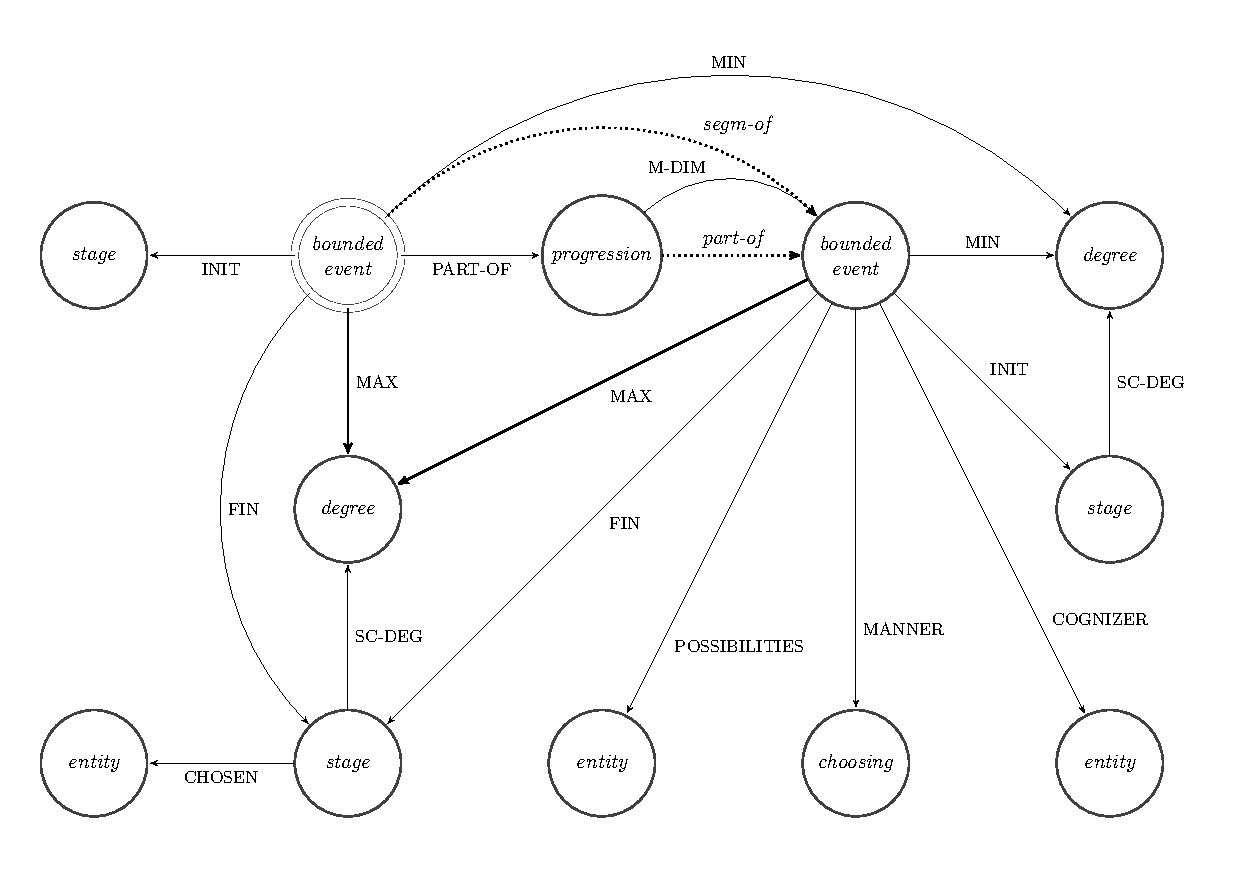
\includegraphics[width=.95\textwidth,trim=0 0 0 30]{dovybiratpf.pdf}
\caption{Graph representation of the verb \textit{dovybirat'}$^{\PF}$ `to finish electing'\label{graph:pf}}
\end{figure}

\begin{figure}[p]
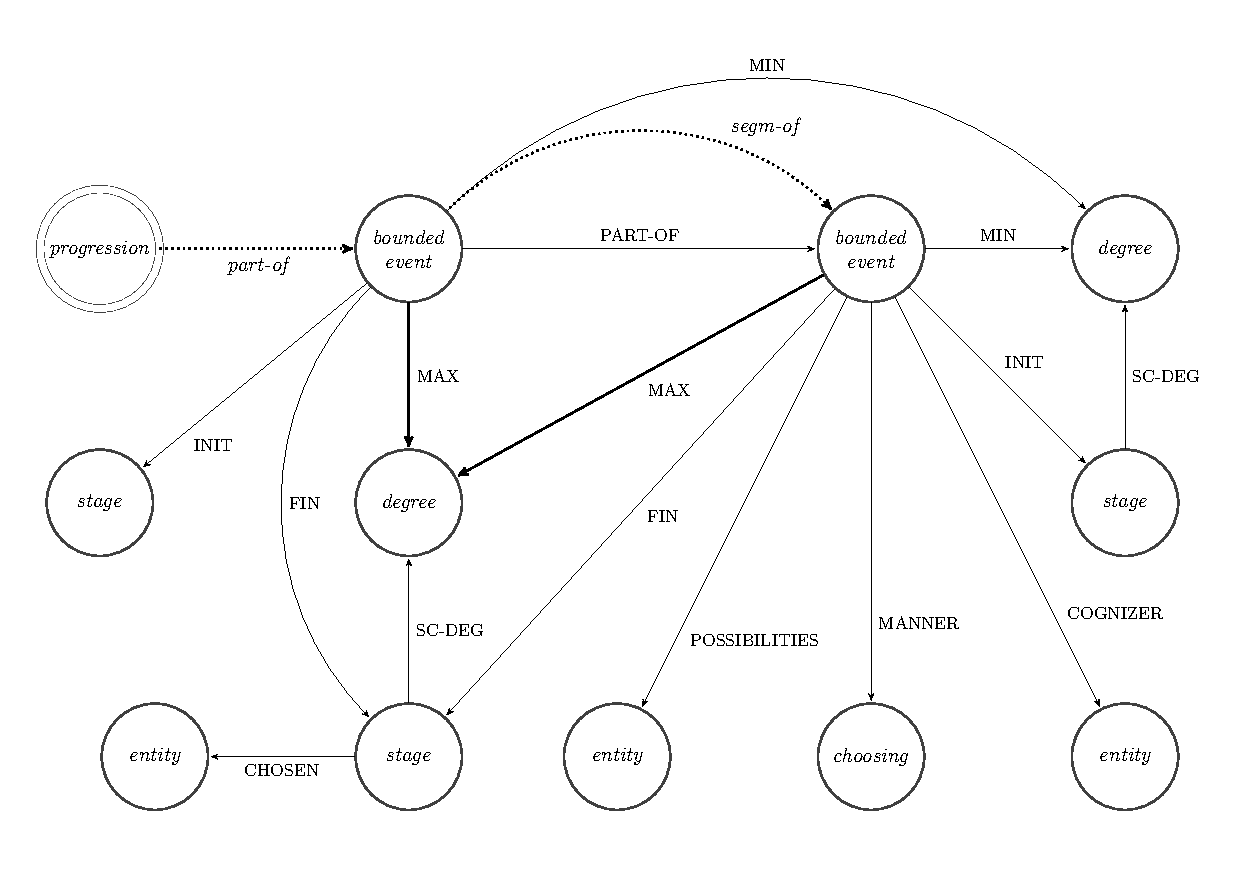
\includegraphics[width=.95\textwidth,trim=0 0 0 20]{dovybiratipf.pdf}
\caption{Graph representation of the verb \textit{dovybirat'}$^{\IPF}$ `to be finishing electing'\label{graph:ipf}}
\end{figure}

The second frame, shown on \figref{graph:ipf}, shares a lot with the first one. However, the crucial difference can be immediately seen: the central node (marked with the double border of the circle) is now of type \textit{progression,} which provides an indication that the verb is imperfective. This is the case when the imperfective suffix is attached on the last step of the derivation. The derived verb, thus, denotes a partial event of electing that is, in turn, a segment of the whole electing event that contains its final stage. The attributes of the core electing event remain the same.

The frame semantic analysis of Russian prefixation system that I develop in Chapter~\ref{Chapter7} illustrates the power and flexibility of the formalism: with basic and easily readable semantics I manage not only to provide the exact interpretation of a given prefixed verb in context, but also block unwanted derivations of complex verbs as well as prevent combinations of verbs with inappropriate direct objects and measure phrases.

I then implement the proposal using XMG 2 \citep{Petitjean:16}. In Chapter~\ref{Chapter8}, I show parts of the implementation and discuss technical details. Due to the current restrictions with respect to the tools available for parsing, I only implement a small fragment that consists of six prefix usages, one verbal base, the imperfective suffix, and one noun that can serve as a direct object, supplying two different scales. The output of the compiler consists of verb models that include various affixes. Each model is accompanied by a tree that shows its internal structure, a set of syntactic properties (including aspect), and a frame that represents the  semantics of the verbal phrase. This allows to check the predictions of the account I propose without the risk of overlooking an unwanted derivation or of making a mistake during the derivation of the representation of a complex verb. This is extremely important if one wants to explore verbs that contain three and more derivational affixes.

In order to see how well my analysis does with respect to predicting the \mbox{(non-)}\linebreak[3]existence of certain affix combinations, I compare the output of my analysis against the proposal by \citet{Tatevosov:09}. For this, I implement the syntactic restrictions for prefix attachment for the same grammar fragment. I then analyse all the models produced by the two implementations and calculate precision and recall. The comparison shows that both approaches rather accurately describe situations with one or two affixes, but both precision and recall of the model built following the proposal of \citet{Tatevosov:09} get low values due to the incorrect predictions of the existence of more complex verbs. As for the implementation of the approach I propose, it continues to deliver accurate predictions beyond two affix situations. In addition, the pragmatic reasoning I propose fine-tunes the system and allows to explain the non-existence of extra models produced by the implementation. From this it follows that with a three component analysis of Russian prefixation that I advocate in this thesis one can achieve full precision and recall in predicting the existence of complex verbs that are not lised in the dictionaries.\largerpage

In sum, in this thesis I develop a complex system that allows to explain Russian prefixation and predict existence, aspectual properties, and semantics of complex verbs. The crucial idea of the analysis is the interaction between syntax, semantics, and pragmatics. While all the components are kept simple, their combination allows to explain subtle distinctions and cases that seem exceptional when all the work is assigned to one linguistic module. An important property of the analysis is the possibility to implement it, which is partially performed in this work.
 % Introduction
% Chapter 2

\chapter{A novel approach to the analysis of Russian complex verbs} % Write in your own chapter title
\label{Chapter2}
%\lhead{Chapter 2. \emph{A novel approach to the analysis of Russian complex verbs}} 
This chapter is dedicated to establishing the basis for the rest of the work. I consider the careful accumulation of data to be an essential starting step for any theoretical work. After a brief introduction to Russian aspect, in Section~\ref{section:new:biaspectual}\footnote{The data I present in this section and the new test for perfectivity are also published as \citealt{ZinovaFilip:13, ZinovaFilip:14b}.} I show that this step has not been done properly so far. As a consequence, an important bit of data has been missed in the earlier studies on Russian prefixation. Unfortunately, some commonly assumed features of the existing analyses do not allow for this data to be accommodated, and a global revision is required.
 
%There are three main parts of this chapter. In the first part of the chapter, Section~\ref{section:new:biaspectual} I will provide data on complex verbs following a certain pattern and discuss the tests that allow us to identify those verbs as been biaspectual. Those kind of verbs are predicted to be non-existent by the syntactic theories of prefixation, as will be shown here and also later in more details in Chapter~\ref{Chapter4}.  

To avoid such problems in the future, I start with the data collection methodology.
In Section~\ref{section:graph}, I discuss the derivational graph as a structure that allows to find and store the data relevant for the Russian verbal prefixation system. I also show how the derivational graph can be used to identify the aspect of any verb in the graph on the basis of the structure of the incoming edges. As a continuation of this topic, in the third part of the chapter, Section~\ref{section:new:perfectivity}, I discuss different cases that challenge the common claim that prefixation as the last step of the derivation leads to the perfective aspect of the derived verb. On this basis I update the procedure of determining the aspect of the verb in the graph.  

%TODO: do I need this?
The last topic to be discussed in this chapter is the connection between verbal prefixation, aspect, and telicity, which will be done in Section \ref{section:new:telicity}). 


\section{The Russian aspectual system and biaspectual verbs}\label{section:new:biaspectual}
This section is organized as follows. In the first part, Section~\ref{subsection:basic}, I provide basic information about aspect in Russian.  In Section~\ref{subsection:bi:data} I present new data: a class of prefixed biaspectual verbs constructed according to a productive pattern. Next, in Section~\ref{subsection:bi:predictions}, I provide an overview of how such verbs are treated by current theories of Russian prefixation. Afterwards, in Section~\ref{sec:tests:old}, I discuss the standard tests used in the literature to determine the aspect of a given verb and show that all of them fail to distinguish between imperfective and biaspectual verbs. In Section~\ref{sec:tests:new} I suggest a new positive test for perfectivity and in Section~\ref{subsection:bi:apply}, this new test is applied to the problematic class of verbs.
%%%TODO: more concrete about what has been published!

\subsection{Basic facts}\label{subsection:basic}
Aspectual distinctions\is{aspect} are referred to by various names: boundedness \citep{Avilova:76, Jakobson:57, Paducheva:96, Talmy:00}, totality \citep{Forsyth:70, Bondarko:71, Comrie:76, Dickey:00, Maslov:65}, closure \citep{Timberlake:82}, closed vs. open aspect \citep{Janda:07a}, among other names. Traditionally, the term ``aspect" (in Russian, \textit{vid}) in Slavic linguistics is used to refer to a grammatical category with two values: perfective and imperfective. In a basic case perfective verbs denote complete situations while imperfective verbs are used to refer to partial situations, habitual events, and states. This said, imperfective verbs can also be used to describe complete events in the past, e.g., when used in ``historical present''. 

The category of grammatical aspect is related to the morphological structure of the verb. Perfective verbs are assumed to be derived from imperfective ones by means of \isi{prefixation}, as illustrated in the example~\ref{ex:asppair}. This assumption is based on the fact that most morphologically basic verbs in Russian are imperfective \citep[see, e.g.,][]{Isachenko:60, Forsyth:70}. However, a small amount of unaffixed verbs are perfective (\citealt{Isachenko:60} lists about 30 of them). Some examples are given in \ref{ex:unprefperf}.

\exg.\label{ex:asppair}pisat'\textsuperscript{\IPF} - napisat'\textsuperscript{\PF}\\
`write' - `write'\\

\exg.\label{ex:unprefperf}brosit'\textsuperscript{\PF}, kupit'\textsuperscript{\PF}, dat'\textsuperscript{\PF}\\
'throw' `buy' `give'\\

Perfective verbs can also be derived by other morphological means than prefixation: for example, semelfactive perfective verbs \is{semelfactive} such are those listed in \ref{ex:semelfactive} are formed by the attachment of the suffix \textit{-nu-} to the respective imperfective base verbs \textit{prygat'} `to jump', \textit{morgat'} `to blink', and \textit{stu\v{c}at'} `to knock'.

\exg.\label{ex:semelfactive}prygnut'\textsuperscript{\PF}, morgnut'\textsuperscript{\PF}, stuknut'\textsuperscript{\PF}\\
{'jump (once)'} {`blink (once)'} {`knock/hit (once)'}\\

Although prefix attachment is related to a change of the aspect of the verb, it also often leads to a shift in the lexical meaning. When there seems to be no (obvious) shift, the perfective and the imperfective verbs are said to form an \textit{aspectual pair}. In \cite{Rosenthal:76} the following definition of an \isi{aspectual pair} is given (my translation from Russian):
\begin{definition}\label{def:pair}
An \isi{aspectual pair} is a pair formed by an imperfective verb and a perfective verb that are lexical-semantically identical.
\end{definition}
\noindent An \isi{aspectual pair} can be formed in the following ways:

\begin{enumerate}[noitemsep]
\item by \isi{suffixation} with possible alternations in the verbal stem (ex.~\ref{pair1});
\item by \isi{prefixation} (ex.~\ref{pair2});
\item by an alternation of the thematic vowel (possibly with a consonant alternation in the verbal stem, ex.~\ref{pair3});
\item stress shift (ex.~\ref{pair4});
\item formation from different stems (suppletive aspectual pairs, ex.~\ref{pair5}).
\end{enumerate}

\ex.\ag.\label{pair1}perepisat'\textsuperscript{\PF} - perepisyvat'\textsuperscript{\IPF}\\
rewrite - rewrite\\
\bg.\label{pair2}delat'\textsuperscript{\IPF} - sdelat'\textsuperscript{\PF}\\
do - do\\
\bg.\label{pair3}vstretit'\textsuperscript{\PF} - vstre\v{c}at'\textsuperscript{\IPF}\\
meet - meet\\
\bg.\label{pair4}nas\'ypat'\textsuperscript{\PF} - nasyp\'at'\textsuperscript{\IPF}\\
meet - meet\\
\bg.\label{pair5}brat'\textsuperscript{\IPF} - vzjat'\textsuperscript{\PF}\\
take - take\\

From \defref{def:pair} follows that when one member of an \isi{aspectual pair} substitutes the other, this should not lead to any change in the semantics of the sentence, as is shown in ex.~\ref{ex:Vasya}.

\ex.\label{ex:Vasya}\ag. Vasya delal\textsuperscript{\IPF} {doma\v{s}neje zadanije}.\\
Vasya didx homework\\
\trans `Vasya was doing/did his homework.'
\bg. Vasya sdelal\textsuperscript{\PF} {doma\v{s}neje zadanije}.\\
Vasya did homework\\
\trans `Vasya did his homework.'

The pair model view of Russian verbal prefixation leaves those prefixed verbs that are not part of a pair outside of the system. Together with \citet{Janda:07a}, who argues for a cluster model of Russian verbs, I find the aspectual pair approach problematic. Instead of talking about pairs, I would use the term \textit{\isi{neutral perfective}} for the perfective members of traditional aspectual pairs plus some other verbs (verbs that denote an action that terminated after some time, more details provided in Chapter~\ref{Chapter6}). In Chapters~\ref{Chapter5} and \ref{Chapter6} I will show that the Russian prefixation system cannot be described in terms of aspectual pairs, as in order to obtain the interpretation of a given verb one needs to pay attention to other verbs derived from the same base. This (non)-existence of various prefixed verbs also influences whether a particular prefix (e.g., \Prefix{s-} or \Prefix{na-}) attachment would lead to the formation of a neutral perfective.

For the moment, however, let us concentrate on the verbs that can be viewed as an extreme case of an \isi{aspectual pair}: \isi{biaspectual verbs}. Such verbs can be used both as perfective and imperfective, so they provide a possibility of aspect change with neither semantic change nor formal change.

\subsection{Data}\label{subsection:bi:data}

% (biasectual cluster is underrepresented in \citet{Janda:07a}. E.g., Janda claims that there only Natural and Specialized perfectives are formed from biaspectual verbs. She studies the verb \textit{klassificirovat'} `to classify' but she does not list the verb \textit{poklassificirovat'} `to classify for a while' among its derivatives). 

In this subsection we are going to investigate \isi{biaspectual verbs}. If one opens a book about Russian verbal aspect, one will most probably read that there are two classes of \isi{biaspectual verbs}. The first class is a relatively small group of verbs with historically Slavic roots, such as \textit{\v{z}enit'}\textsuperscript{\PF\slash\IPF} `to marry (off)' or \textit{kaznit'}\textsuperscript{\PF\slash\IPF} `to execute,' \textit{ranit'}\textsuperscript{\PF\slash\IPF} `to wound'. Examples of the usage of the verb \textit{\v{z}enit'}\textsuperscript{\PF\slash\IPF} `to marry (off)' in different aspects are provided in \ref{ex:biaspectual:native}. The second class of biaspectual verbs are loaned verbs ending in \textit{-ovat'}, such as \textit{arestovat'}\textsuperscript{\PF\slash\IPF} `to arrest' or \textit{reformirovat'}\textsuperscript{\PF\slash\IPF} `to reform'. The biaspectual nature of the verb \textit{reformirovat'}\textsuperscript{\PF\slash\IPF} is revealed in the example \ref{ex:biaspectual:borrowed}. 

\ex.\label{ex:biaspectual:native}
\ag.Ka\v{z}etsja, kogda ix \v{z}enili\textsuperscript{\IPF}, Xalima byla o\v{c}en', o\v{c}en' krasivaja.\\
seems when they.\glb{acc} marry.\glb{pst.pl} Xalima be.\glb{pst.sg.f} very very beautiful.\glb{sg.f.nom}\\
\trans `It seems that when they were getting married, Xalima was very, very beautiful.' \hfill Andrej Volos, \textit{Sirijskie rozy} (1999)
\bg.``Devo\v{c}ki'' povydavali do\v{c}ek zamu\v{z}, \v{z}enili\textsuperscript{\PF} synovej, stali babu\v{s}kami.\\
``girl.\glb{pl.nom}'' po.vy.give.imp.\glb{pst.pl} daughter.\glb{pl.acc} marry marry.\glb{pst.pl} son.\glb{pl.acc} become.\glb{pst.pl} grandmother.\glb{pl.inst}\\
\trans `{``}Girls'' married off their daughters, married off their sons, became grandmothers.'\hfill\hbox{Bella Ezerskaja, \textit{Odessa, Literaturnyj muzej} (2003)}

\ex.\label{ex:biaspectual:borrowed}\ag.Stranno, 10 let reformirovali\textsuperscript{\IPF}, i opjat' v na\v{c}ale?\\
strange 10 year.\glb{pl.gen} reform.\glb{pst.pl} and again in beginning.\glb{sg.prep}\\
\trans `It's strange, they have reformed it for 10 years and are again in the beginning of this process?'
\hfill izvestia.ru
\bg.My reformirovali\textsuperscript{\PF} sistemu gosudarstvennoj slu\v{z}by, proveli pensionnuju reformu.\\
we reform.\glb{pst.pl} system.\glb{sg.acc} public service, conduct.\glb{pst.pl} pensionary.\glb{sg.f.acc} reform.\glb{sg.acc}\\
\trans `We have reformed the public service system, conducted a pensionary reform.'
\hfill izvestia.ru

Russian morphological tradition treats biaspectual verbs as verbs with syncretic paradigms. According to \citet{Galton:76}, \citet{Rosenthal:76}, \citet{Shvedova:82}, \citet{Certkova:96}, \citet{ZaliznjakShmelev:00}, and \citet{Janda:07a}, among others,  these verbs can be used as perfective and imperfective verbs, depending in the context. In the case of biaspectual verbs, context and information structure are crucial for aspect determination, as illustrated in the example~\ref{ex:biasp}. In the case of sentence \ref{ex:biasp:a}, the default reading (with unmarked intonation) is that of an unfolding event (imperfective). As for the second sentence \ref{ex:biasp:b}, the default reading is that of a completed event. (In both cases the other aspect is available if the intonation pattern is changed.)

\ex.\label{ex:biasp}\a.\label{ex:biasp:a}\gll Na central'noj plo\v{s}\v{c}adi kaznili\textsuperscript{\IPF} prestupnika.\\
on central square hang.\glb{pst.pl} criminal\glb{.sg.acc}\\
\glt `On the central square they were hanging a criminal.'
\b.\label{ex:biasp:b} \gll Prestupnika kaznili\textsuperscript{\PF} na central'noj plo\v{s}\v{c}adi.\\
criminal.\glb{sg.acc} hang.\glb{pst.pl} on central square\\
\glt `The criminal was hanged on the central square.'

For more details about the specific properties of both native and loaned \isi{biaspectual verbs} see, e.g. \citet{Isachenko:60}, \citet{Avilova:68}, \citet{Skott:79}, \citet{Gladney:82}, \citet{Certkova:98}, \citet{Jaszay:99}, \citet{Anderson:02}, \citet{Timberlake:04}, and \citet{Janda:07a}. 

To provide some background, let me mention two studies investigating the frequency of native \isi{biaspectual verbs} relative to loaned \is{loaned verbs} ones. According to a statistical study by \citet{Certkova:98}, borrowed biaspectual verbs constitute more than 90\% of all the biaspectual verbs in Russian. This result is obtained on the basis of the data collected from the \citet{Ozegov:90} dictionary. According to another study, \citet{Anderson:02}, completed on the data from the \citet{Zaliznjak:77} dictionary, the percentage of borrowed biaspectual verbs with respect to all biaspectual verbs is even higher, about 95\%. It is important to note that these studies are concerned almost exclusively with nonprefixed biaspectual verbs (as these are listed in the dictionaries). So these numbers indicate only how many \isi{biaspectual verbs} of each type exist in the language as documented by the dictionaries, but not how often each of the two types is used or how productive they are in the derivational morphology system.

What is not included in the above-mentioned studies are prefixed (and suffixed) \isi{biaspectual verbs}. As is evident from a corpus-based study by \citet{Borik:12}, such verbs do exist. They do not seem to be very common: in the data that is included in the Open Source Lexical Information Network (OSLIN) for Russian, only 0.25\% of the prefixed verbs are biaspectual. However, the database is constructed on the basis of the dictionary data from two explanatory dictionaries: \citet{Ushakov:50} and \citet{OzegovShvedova:92}, so it is far from exhaustive for the purpose of studying prefixed verbs. Dictionaries cover a range of verbs with a single prefix, but almost never include more complex verbs with stacked prefixes. 

Some more information about prefixed biaspectual verbs \is{prefixation} can be found in the Russian Grammar by \citet{Shvedova:82}, where it is stated that biaspectual verbs that contain a prefix can be formed by loaned prefixes \textit {de-}, \textit {dis-}, and \Prefix{re-}, or can be contained among the verbs with other prefixes. As examples \citet{Shvedova:82} provides such verbs as  \textit{dooborudyvat'}\textsuperscript{\IPF\slash\PF} `to finish equipping,' \textit{nedoispolzovat'}\textsuperscript{\IPF\slash\PF} `to not use to the full extent,' and \textit{pererasxodovat'}\textsuperscript{\IPF\slash\PF} `to spend more than was allowed,' also stating that their quantity is marginal. 

I claim that prefixed biaspectual verbs constitute an open class of lexical items, as they can be constructed along productive patterns. Let us for the moment examine one such group\footnote{More groups of biaspectual verbs are provided in Section~\ref{section:new:perfectivity}.}, namely, the \isi{biaspectual verbs} that are formed with the suffix \textit{-iva-/-yva-} and two or more prefixes, where the outermost is the completive:
\ex. \label{form:do}do-PREF$^{+}$-ROOT-yva-t'

Here are some illustrative examples of the verbs that are constructed following the pattern in \ref{form:do}: 
\ex.\label{ex:prefixedverbs}\a.\textit{do-pere-za-pis-yva-t'} `to finish/be finishing writing down again', 
\b. \textit{do-pere-stra-iva-t'} `to finish/be finishing rebuilding',
\b. \textit{do-vy-\v{s}-iva-t'} `to finish/be finishing embroidering',
\b. \textit{do-za-pis-yva-t'} `to finish/be finishing writing down', 
\b. \textit{do-pere-pis-yva-t'} `to finish/be finishing rewriting/copying', 
\b. \textit{do-za-kaz-yva-t'} `to finish/be finishing ordering'.

All the components in Scheme~\ref{form:do} are crucial for obtaining a biaspectual verb. First, verbs that contain \Prefix{do-} as the outermost prefix, but do not contain the imperfective suffix, as in \ref{ex:scheme:perfective}, are clearly perfective. Second, verbs where there is no other prefix between the prefix \Prefix{do-} and the root, as in \ref{ex:scheme:imperf}, are imperfective.

\ex.\label{ex:scheme:perfective}do-PREF$^{+}$-ROOT-t'
\a.\textit{do-pere-pis-a-t'}\textsuperscript{\PF} `to finish writing again', 
\b. \textit{do-pere-stro-i-t'}\textsuperscript{\PF} `to finish rebuilding',
\b. \textit{do-za-kaz-a-t'}\textsuperscript{\PF} `to finish ordering'.

\ex.\label{ex:scheme:imperf}do-ROOT-yva-t'
\a.\textit{do-pis-yva-t'}\textsuperscript{\IPF} `to finish/be finishing writing', 
\b. \textit{do-straj-iva-t'}\textsuperscript{\IPF} `to finish/be finishing building',
\b. \textit{do-kaz-yva-t'}\textsuperscript{\IPF} `to prove/be proving'.

Depending in the context, the verbs in \ref{ex:prefixedverbs} are assigned to either the imperfective aspect (examples \ref{ex:doperezaimp} and \ref{ex:dopereimp}) or the perfective aspect (examples \ref{ex:doperezapf} and \ref{ex:doperepf}). 

\ex. \ag. \label{ex:doperezaimp}V dannyj moment doperezapisyvaju e\v{s}\v{c}e 2 pesni.\\
in given moment do.pere.za.write.imp.\glb{1.sg} also 2 songs\\
\trans `I'm currently finishing rerecording two more songs.'\hfill metalrus.ru
\bg. \label{ex:doperezapf}Doperevela ``Talisman'' \v{S}andmaulej i doperezapisyvala sobstvennye pesni.\\
do.translate.\glb{pst.f.sg} ``Talisman'' \v{S}andmaul.\glb{gen} and do.pere.za.write.imp.\glb{pst.f.sg} own songs.\\
\trans `I finished translating ``Talisman'' by the group ``\v{S}andmaul'' and finished rerecording my own songs.'

In \ref{ex:doperezaimp} the verb \textit{doperezapisyvaju} `I am finishing rewriting' behaves like an imperfective verb, because it has a progressive interpretation triggered by the adverbial \textit{v dannyj moment} `currently' (standard tests for determining the verbal aspect are discussed in Section~\ref{sec:tests:old}). Another form of the same verb, \textit{doperezapisyvala} `I finished rerecording', behaves like a perfective verb in \ref{ex:doperezapf}. This is revealed by the conjunction with the perfective verb \textit{doperevela} `finished translating' (see the more detailed explanation in Section~\ref{sec:tests:new}).

\ex.\ag.\label{ex:dopereimp}Ja skol'ko ni doperestraival, ljudi v itoge tratili bol'\v{s}e, \v{c}em na novuju postrojku.\\
I how.much ever do.pere.build.imp.\glb{pst.sg.m}, people in total spent more then on new bulding.\\
\trans `Every time I was rebuilding something, in the end the clients spent more than they would have paid for the new building.'\\
\hbox{}\hfill\hbox{www.kharkovforum.com}
\bg.\label{ex:doperepf}Vot tol'ko traktir doperestraivaju, proekt sdam, diplom polu\v{c}u...\\
here only tavern do.pere.build.imp.\glb{pres.1.sg}, project hand.in.\glb{pres.1.sg}, diploma receive.\glb{pres.1.sg}\\
\trans `I will just first finish rebuilding the tavern, then hand in the project and receive the diploma...'\\
\hbox{}\hfill\hbox{Elena Berezovskaja, \textit{Traktir pod ``znakom ka\v{c}estva''} (2013)}

In \ref{ex:dopereimp} the verb \textit{doperestraival} `was finishing rebuilding' is used as an imperfective verb with an iterative meaning and in \ref{ex:doperepf} the same verb \textit{doperestraivaju} `I will finish rebuilding' can only be assigned to the perfective aspect because it has future reference in the nonpast tense.

We can also see that verbs with the structure following Scheme~\ref{form:do} behave differently with respect to what is traditionally considered to be a telicity test than verbs that contain either a single prefix and an imperfective suffix or only prefixes (for example, the verbs in \ref{ex:scheme:perfective} and \ref{ex:scheme:imperf}). Verbs with just one prefix and the imperfective suffix like \textit{dopisyvat'} `to finish/be finishing writing', that are clearly imperfective, are incompatible with a prepositional time measure phrase \textit{za $\alpha$ \v{c}asov} `in $\alpha$ hours' (\ref{ex:1preftel} is ungrammatical).\footnote{As pointed out by an anonymous reviewer, in a special context the verb can acquire a planned future interpretation which would allow for a \Prefix{za-}headed time measure phrase as describing the expected completion time. There is still an asymmetry between \ref{ex:1preftel} and \ref{ex:2preftel}.} Verbs that do not have the imperfective suffix in their structure and are clearly perfective, as \textit{dozapisat'} `to finish writing down/recording' are not compatible with accusative time measure phrases (see \ref{ex:3pref}). In contrast to this, verbs like \textit{dozapisyvat'} `to finish/be finishing writing down/recording', that have the structure given in \ref{form:do}, are perfectly acceptable with either accusative or prepositional time measure phrases (both \ref{ex:2preftel} and \ref{ex:2prefatel} are fine).

\ex.\label{ex:1pref}\ag.*Ja dopisyvaju pesnju za dva \v{c}asa.\label{ex:1preftel}\\
I do.write.imp.\glb{pres.1.sg} song in two hours\\
\bg. \label{ex:1prefatel}Ja dopisyvaju pesnju u\v{z}e dva \v{c}asa.\\
I do.write.imp.\glb{pres.1.sg} song already two hours\\
\trans `I'm finishing writing the song for two hours already.'

\ex.\label{ex:3pref}\ag. \label{ex:3preftel}Ja dozapi\v{s}u pesnju za dva \v{c}asa.\\
I do.za.write.\glb{pres.1.sg} song in two hours\\
\trans `I will finish recording the song in two hours.'
\bg.*Ja dozapi\v{s}u pesnju u\v{z}e dva \v{c}asa.\label{ex:3prefatel}\\
I do.za.write.\glb{pres.1.sg} song already two hours\\

\ex.\label{ex:2pref}\ag. \label{ex:2preftel}Ja dozapisyvaju pesnju za dva \v{c}asa.\\
I do.za.write.imp.\glb{pres.1.sg} song in two hours\\
\trans `I will finish recording the song in two hours.'
\bg. \label{ex:2prefatel}Ja dozapisyvaju pesnju u\v{z}e dva \v{c}asa.\\
I do.za.write.imp.\glb{pres.1.sg} song already two hours\\
\trans `I'm finishing recording the song for two hours already.'

I have to note that the variability of the perfective and imperfective uses of biaspectual verbs is a matter of some disagreement. Not all the speakers can access both the perfective and the imperfective variant of the verbs in \ref{ex:prefixedverbs}. For instance, according to some of the speakers I have consulted with, \textit{dozapisyvat'} `to be finishing/finish writing down' cannot be used as a perfective verb, i.e., it is not biaspectual. However, such speakers would also agree that the structurally similar verb \textit{dovy\v{s}ivat'} `to be finishing/finish embroidering' can, indeed, be used as a perfective verb in contexts like~\ref{ex:dovysh}.
\exg.\label{ex:dovysh}Planiruju pristupit' k rabote \v{c}erez dve nedeli, kak tol'ko dovy\v{s}ivaju ``Lesnuju zarju''.\\
plan.\glb{pres.1.sg} start.inf to work over two weeks, as only do.vy.sew.imp.\glb{pres.1.sg} ``Forest dawn''\\
\trans `I plan to start the work in two weeks' time; as soon as I will have finished embroidering ``Dawn in the forest''.'
\hfill eva.ru/R1kYl

\subsection{Predictions of the existing approaches}\label{subsection:bi:predictions}
Let me show how contemporary syntactic accounts of Russian verbal prefixation determine the aspect of the verbs in \ref{ex:prefixedverbs}. First I will provide a brief overview of the analyses proposed in the literature \citep{Ramchand:04, Svenonius:04a, Svenonius:04b, Romanova:06, Tatevosov:07, Tatevosov:09}. The key idea that drives syntactic approaches to Russian prefixation is the division of the prefix usages into lexical/internal and superlexical/external. An extensive discussion of this distinction and a detailed overview of the proposals will follow in Chapter~\ref{Chapter4}. What matters now is that superlexical prefixes are claimed (see, e.g., \citealt[229]{Svenonius:04b}) to not allow the formation of secondary imperfectives, occasionally stack outside (never inside) lexical prefixes, and select for imperfective stems.

In syntactic approaches to Russian prefixation the internal structure of complex verbs is represented by means of syntactic trees. In these trees lexical and superlexical prefixes occupy different positions, and the aspect of the verb is determined by the properties of the highest affix in the structure. For example, according to \citealt{Svenonius:04b} (see also the summary in \citealt{Svenonius:12}), complex verbs have the following structure: lexical prefixes originate inside \textit{v}P; superlexical prefixes originate outside \textit{v}P; lexical and superlexical prefixes that disallow secondary imperfectivization are separated by Asp in the syntactic structure; and some exceptional superlexical prefixes are merged (sometimes) below the Asp.

Concerning the way the aspect of a complex verb is determined, the following rules, given in \cite{Borer:13}, implicitly emerge from \citet{Ramchand:04}, \citet{Romanova:04}, and \citet{Svenonius:04b}:
\ex.\label{bor}\a. V $\rightarrow$ {imperfective}\footnote{In addition to listed biaspectual and perfective simplex verbs.}
\b. Prefix + V $\rightarrow$ {perfective}
\b. V + Semelfactive $\rightarrow$ {perfective}
\b. Prefix + V + S-imperfective/Hab $\rightarrow$ {imperfective}
\b. Prefix + (Prefix + V + S-imperfective/Hab) $\rightarrow$ {perfective}

So it is generally assumed (see (a)) that basic nonaffixed verbs are imperfective (with a closed list of exceptions). When prefixed (b), these verbs become perfective. They also become perfective if a semelfactive suffix is added (c). If a prefixed perfective verb (output of (b)) is suffixed with the imperfective suffix, the aspect of the verb changes to imperfective (d). If a second prefix is added to such a verb, the output is perfective (e).

In further developments we see a shift of focus from the bipartite distinction to the split of the whole class of prefixes into more than just two main classes. \citet{Tatevosov:07}, for example, proposes a three-way classification of verbal prefixes, arguing for the existence of intermediate prefixes, in addition to lexical and superlexical ones. The group of the intermediate prefixes is constituted by completive \textit{do}- and repetitive \textit{pere}-. In a later work, \citet{Tatevosov:09} returns to a bipartite distinction between lexical and superlexical prefixes, but subdivides the superlexical class into three groups: selectionally limited prefixes (delimitative \Prefix{po-}, cumulative \Prefix{na-}, distributive \Prefix{pere-}, inchoative \Prefix{za-}), positionally limited prefixes (completive \Prefix{do-}, repetitive \Prefix{pere-}, and attenuative \Prefix{pod-}), and the left periphery prefix (distributive \Prefix{po-}).

If we take into account the proposals by \citet{Tatevosov:07, Tatevosov:09}, the schema in \ref{bor} is completed with the following rule (f), where (f) must be applied instead of (e) in cases when the outermost prefix is either \textit{intermediate} \citep{Tatevosov:07} or \textit{positionally limited} \citep{Tatevosov:09}: 
\ex.[]\a.[f.] (PosLim/ItmPrefix + Prefix* + V) + S-imperfective/Hab $\rightarrow$\\ \textit{imperfective} 

Examples \ref{ex:pred} illustrate the application of the corresponding rules in \ref{bor}.

\begin{minipage}{0.43\linewidth}
\vspace*{.5\baselineskip}
\ex.\label{ex:pred}\ag.\label{pred1}pisat'\textsuperscript{\IPF}\\
write.\glb{inf}\\
`to write'
\bg.\label{pred2}zapisat'\textsuperscript{\PF}\\
za.write.\glb{inf}\\
`to write down'
\bg.\label{pred3}prygnut'\textsuperscript{\PF}\\
jump.semelf.\glb{inf}\\
`to jump once'

\vspace*{.5\baselineskip}
\end{minipage}%
\begin{minipage}{0.55\linewidth}
\vspace*{.5\baselineskip}
\exg.[d.]\label{pred4}zapisyvat'\textsuperscript{\IPF}\\
za.write.imp.\glb{inf}\\
`to be writing down/to write down'
\bg.[e.]\label{pred5}nazapisyvat'\textsuperscript{\PF}\\
na.za.write.imp.\glb{inf}\\
`to write down a lot'
\bg.[f.]\label{pred6}perezapisyvat'\textsuperscript{\IPF}\\
pere.za.write.imp.\glb{inf}\\
`to be rewriting/to rewrite'

\vspace*{.5\baselineskip}
\end{minipage}

The summary provided by the rules in \ref{bor} reveals the fact that all the existing syntactic approaches predict any given single verb token with a given interpretation to be assigned one aspect (either perfective or imperfective). This comes as a consequence of the fact that the position of each prefix in the syntactic structure is fixed.\footnote{The impossibility of having a syntactic ambiguity for a given verb with a fixed interpretation should not be confused with the situation in which the verb has two meanings, i.e., the case of a genuine lexical ambiguity. In such case, all the approaches discussed predict that each meaning is associated with a different syntactic tree.} 

To illustrate this point, which is crucial for my purposes, let us take as an example the biaspectual verb \textit{dozapisyvat'} `to finish writing/to be finishing writing', that follows the pattern \ref{form:do}. Given the predictions of the syntactic accounts of Russian prefixation, summarized under \ref{bor}, it is clear that these accounts would assign this verb one aspect. At the same time this is exactly the case where different approaches end up with distinct predictions. For such verbs as \textit{dozapisyvat'} `to finish writing/to be finishing writing,' depending in the theory, either the rule (e) or the rule (f) must be applied.

The verb \textit{dozapisyvat'} `to finish writing/to be finishing writing' contains the following derivational morphemes: the superlexical prefix \Prefix{do-} with the completive meaning (see, e.g., \citealt{Svenonius:04a} for classification), the lexical prefix \Prefix{za-} with non-compositional semantic contribution, the stem \textit{-pis-} and the imperfective suffix \textit{-yva-}. 

Following \citet{Svenonius:04b} and rule (e) in schema \ref{bor}, we obtain the tree shown on \figref{tree:sven} for the verb \textit{dozapisyvat'} `to finish writing/to be finishing writing'. The completive prefix \textit{do}- scopes over the imperfective suffix, so the verb must be assigned the perfective aspect. Note that \citet{Svenonius:04b} does not explicitly discuss the characteristics of the prefix \Prefix{do-}. However, in \citet{Svenonius:04a} this prefix is classified as being superlexical and \citet{Svenonius:04b} makes general statements about the properties of the class of superlexical prefixes. In sum, this allows us to conclude that the verb \textit{dozapisyvat'} `to finish writing/to be finishing writing' should be analyzed in the way illustrated by \figref{tree:sven}. The analysis by \citet[357]{Ramchand:04} makes essentially the same predictions.

\begin{figure}
\caption{Tree for \textit{dozapisyvat'} `to (be) finish(ing) writing' according to the proposal in \citet{Svenonius:04b}\label{tree:sven}}
% % 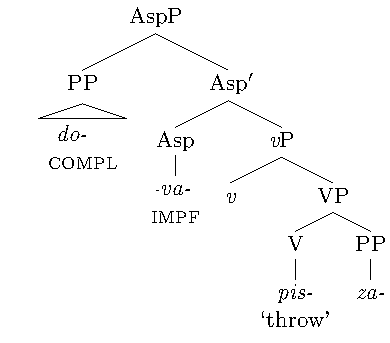
\includegraphics{dozapisyvat-Sven.pdf}
\begin{forest}
[AspP
 [PP [\Prefix{do-}\\\COMPL,align=center,roof]]
 [Asp'
   [Asp [-\textit{yva}-\\\IPF,align=center] ]
        [\textit{v}P
          [\textit{v}]
          [VP
            [V [\textit{pis}-\\`throw',align=center]]
            [PP [\textit{za}-]]
          ]
        ]
 ]
]
\end{forest}
\end{figure}

\begin{figure}
\caption{Tree for \textit{dozapisyvat'} `to (be) finish(ing) writing' according to the proposal in \citet{Tatevosov:07}\label{tree:tat}}
% % 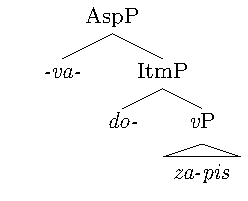
\includegraphics{dozapisyvat-Tat07.pdf}
\begin{forest}
[AspP
 [-\textit{yva}-]
 [ItmP
   [\textit{do}-] [\textit{v}P [\textit{za-pis},roof]]
 ]
]
\end{forest}
\end{figure}

% states, that when a lexical prefix and a superlexical co-occur with the secondary imperfective suffix, the resulting word behaves like a perfective, i.e., the scoping is similar to what was proposed by \citet[ex.~(70)]{Svenonius:03}, corresponding to the rule (e) in the schema above.\\
Contrary to both \citet{Svenonius:04b} and \citet{Ramchand:04}, \citet{Tatevosov:07} arrives at a different aspectual classification of the same verb. This is because according to \citet{Tatevosov:07}, \textit{do}- occupies a special projection for intermediate prefixes so that the resulting syntactic structure is as on \figref{tree:tat}. As we see, the imperfective suffix is in the highest position and the aspect of the whole verb must be imperfective. 

As is shown by the examples above, approaches such as \citet{Svenonius:04b}, \citet{Ramchand:04}, \citet{Romanova:06}, and \citet{Tatevosov:07} predict exactly one syntactic structure for the verb \textit{dozapisyvat'}, as well as for any other verb. This holds even for the most detailed account by \cite{Tatevosov:09}. Here the existence of an exceptional group of superlexical prefix uses is postulated. This group is the group of selectionally limited prefixes and includes delimitative \Prefix{po-}, cumulative \Prefix{na-}, distributional \Prefix{pere-} and inchoative \Prefix{za-}. These prefixes, according to \citet{Tatevosov:09}, can take a position ``above'' or ``below'' the imperfective suffix as long as the source verb is imperfective (which is not allowed in other approaches). However, this fact does not affect the overall prediction that there is a unique syntactic structure assigned to each given complex verb (with fixed interpretation) due to the selectional restriction.

This conclusion is not immediately obvious, so let us consider an example. Verbs that follow the Scheme~\ref{form:do} contain the imperfective suffix and two prefixes, the outermost of which, \Prefix{do-}, is, according to \citet{Tatevosov:09}, selectionally limited (can only be attached to a formally imperfective verb). As selectionally limited prefixes can appear either higher or lower than the imperfective suffix, there seems to be a potential for the structural ambiguity. Examples of such verbs are \textit{zazapisyvat'} `to start writing down/recording' and  \textit{nazapisyvat'} `to write down/record a lot'. It turns out that for such verbs there is a unique order of affix attachment possible, as the second prefix cannot be attached earlier than the imperfective suffix because of the selectional restriction.

One exception to the rule ``one verb -- one structure'' is a modification of \citet{Tatevosov:09} sketched in \citet{Tatevosov:13} that seems to implicitly react to problematic examples first mentioned in \citet{Zinova:12}. \citet{Tatevosov:13} proposes that the completive prefix \Prefix{do-} (for a certain group of Russian speakers) does not have any restrictions on its attachment. If, however, such modification is adopted without further restrictions, the predicted class of biaspectual verbs ends up beeing too large. This problem may be solvable, but, as no solution is offered by the author, I will not discuss this proposal further.

%
%Let us suppose that we modify the syntactically based approaches in such a way that they would allow syntactic ambiguity. Even giving them the benefit of doubt that their analyses can be extended, this still leads to the following problem. Let us consider two verbs following the pattern in (1): dozapisyvat’ ‘to finish writing down’ and dovyshivat’ ‘to finish embroidering.’ These verbs have exactly the same affixes involved: a lexical prefix, a superlexical prefix do- with completive meaning and the imperfective suffix. However, these verbs exhibit a clear difference in their usage: dozapisyvat’ is primary imperfective (about one half of the speakers accept it as being both perfective and imperfective, all accept it as an imperfective verb) while dovyshivat’ is primary perfective (all naïve native speakers that were questioned accept it as a perfective verb and most do not accept it as an imperfective verb). Such behavior is completely unexpected under any syntactic theory, as from the syntactic point of view these verbs are identical and must exhibit the same properties.\\
In sum, the notion of a structural position is helpful in motivating at least certain facts about the formation of complex verbs (as shown by example \ref{ex:pred}). For this reason syntactic approaches were a necessary step in the process of understanding Russian prefixation system. However, the problematic part of these approaches is that, as I have shown, they exclude the existence of biaspectual affixed verbs. The reason for this is that the postulated structural assumptions force a given complex verb to be assigned exactly one structure. This structure, in turn, determines the aspect of the verb independently of any other factors. An attempt to overcome the ``one verb -- one structure'' restriction without subdividing the class of superlexical prefixes even further  \citep{Tatevosov:13} leads to massive overgeneration. The problem, in my view, lies in the assumption of a strict distinction between lexical and superlexical prefixes. In Chapter~\ref{Chapter4} we will discuss in detail properties that are assigned to each class and I will show that there is no evidence for a strict classification, as each property is true of a different set of prefix usages.

\subsection{Diagnostics for aspectual classes}\label{sec:tests:old}
Several tests are commonly used to establish the aspect of a given verb in Russian. Surprisingly, all of them are designed to exclude the possibility that it is perfective. Hence, they focus on the negative formal properties of perfective verbs. The following test set is provided by \citet{Schoorlemmer:95}: 
\ex.\label{tests} \a.[(i)] \label{sttest1} perfective verbs \textit{do not} get an ``ongoing'' interpretation in nonpast tense; 
\b.[(ii)] \label{sttest2} perfective verbs \textit{cannot} be used as complements of phasal verbs (e.g., \textit{na\v{c}at'} `to begin'); 
\b.[(iii)] \label{sttest3} perfective verbs \textit{cannot} form present participles.

\subsubsection{Non-past tense reading test}
This test is concerned with the interpretation possibilities for verbs with present tense morphology. Perfective verbs, as illustrated by \ref{ex:fut:2}, cannot receive present progressive interpretation, as opposed to imperfectives \ref{ex:fut:1}.

\ex.\label{ex:fut}\ag.\label{ex:fut:1}Vasja pi\v{s}et\textsuperscript{\IPF} pis'mo.\\
Vasja write.\glb{pres.3.sg} letter\\
`Vasja is writing a letter.'
\bg.\label{ex:fut:2}Vasja napi\v{s}et\textsuperscript{\PF} pis'mo.\\
Vasja na.write.\glb{pres.3.sg} letter\\
`Vasja will write a letter.'
 
\subsubsection{Phase verbs}
There is a group of verbs that can take either nominals or infinitives as their complements. These verbs are called \textit{phase verbs}. In \cite{Borik:02} the following list of such verbs is provided:
\begin{itemize}[noitemsep]
\item \textit{na\v{c}inat'} `begin'
\item \textit{prodol\v{z}at'} `continue'
\item \textit{zakan\v{c}ivat'} `finish'
\item \textit{kon\v{c}at'} `finish'
\item \textit{perestavat'} `stop'
\end{itemize}
The test uses the fact that only imperfective verbs can be complements of the phrase verbs, as illustrated by \ref{ex:phrase}.

\ex.\label{ex:phrase}\ag.Vasja na\v{c}al pisat'\textsuperscript{\IPF}/*napisat'\textsuperscript{\PF} pis'mo.\\
Vasja began write.\glb{inf} letter\\
Vasja began writing a letter
\bg.Ma\v{s}a zakon\v{c}ila \v{c}itat'\textsuperscript{\IPF}/*pro\v{c}itat'\textsuperscript{\PF} knigu.\\
Masha finished read.\glb{inf} book\\
Masha finished reading the book

\subsubsection{Present participles}
\cite{Borik:02} offers a test for perfectivity based on the fact that present participles can only be derived from imperfective verbs. There are four kinds of participles in Russian, as shown on Table~\ref{table:part}. They are characterized by two properties: tense (present or past) and voice (active or passive).
\begin{table}
\caption{Verbal participles in Russian}\label{table:part}
\begin{tabularx}{\textwidth}{lQQ}
\lsptoprule
 & active & passive\\\midrule
  present &  \v{c}it-a-ju\v{s}\v{c}-ij `reading' & \v{c}it-a-em-yj `being read' \\
  past & \v{c}it-a-v\v{s}-ij `reading' (past); pro-\v{c}it-a-v\v{s}-ij `having read' & \v{c}it-a-nn-yj `being read' (past); pro-\v{c}it-a-nn-yj `having been read'\\
\lspbottomrule
\end{tabularx}
\end{table}

Present active participles  (PAPs) are more common than present passive participles, so they are more convenient to use for aspect testing. As they denote ongoing progressive events, they can only be formed from imperfective stems. Examples~\ref{ex:part1} and \ref{ex:part2} illustrate how the test can be applied: \ref{ex:part11} shows the formation of a present active participle of the imperfective verb \textit{\v{c}itat'} `to read'. Example \ref{ex:part12} shows that in case of the perfective verb \textit{pro\v{c}itat'} `to read through' such formation is not possible.\footnote{There are, however, some participles that are formed from perfective verbs and are widely accepted (although not included in the literary norm), such as \textit{zainteresuju\v{s}\v{c}ij} `that will interest you' as evidenced by \ref{ex:PFP}.
\exg.\label{ex:PFP}vy mo\v{z}ete samostojatel'no zapisat'sja i pose\v{s}\v{c}at' zainteresuju\v{s}\v{c}ij vas kurs\\
you.\glb{nom} can {on your own} za.write.\glb{inf.refl} and visit.\glb{inf} za.interest.\glb{pap.sg.m} you.\glb{acc} course.\glb{acc}\\
\trans `you can on your own inscribe and visit a course that you will find interesting'\\\hbox{} \hfill \hbox{\url{www.nstu.ru}}

} Example \ref{ex:part2} illustrates the same distribution for the verbs \textit{pisat'}\textsuperscript{\IPF} `to write' and \textit{napisat'}\textsuperscript{\PF} `to write down'.

\ex.\label{ex:part1}\ag.\label{ex:part11}\v{c}it-a-ju\v{s}\v{c}-ij\\
read\textsuperscript{\IPF}.\glb{PAP.sg.m}\\
reading
\bg.\label{ex:part12}*pro-\v{c}it-a-ju\v{s}\v{c}-ij\\
pro.read\textsuperscript{\PF}.\glb{PAP.sg.m}\\

\ex.\label{ex:part2}\ag.\label{ex:part21}pi\v{s}-u\v{s}\v{c}-ij\\
write\textsuperscript{\IPF}.\glb{PAP.sg.m}\\
writing
\bg.\label{ex:part22}*na-pi\v{s}-u\v{s}\v{c}-ij\\
write\textsuperscript{\PF}.\glb{PAP.sg.m}\\
\z.


\subsection{A positive test for perfectivity}\label{sec:tests:new}
As we have just seen, perfective verbs are commonly distinguished from imperfectives by tests that specify the properties that perfectives fail to have. While these tests delimit perfective verbs, they cannot distinguish between imperfective and biaspectual verbs. Based on the previous aspect research, there seem to be two more possible candidate tests for perfectivity: one relies on past passive participle formation and the other makes use of the properties of the narrative sequence. %We will ultimately show that neither of them works. 

According to the first potential test, past passive participles (PPPs) can only be formed from perfective verbs. For example, in the pairs of verbs shown in \ref{pair} while the perfective member sanctions the derivation of a PPP \ref{ppp2}, the imperfective one is not supposed to do so \ref{ppp1}.
\exg.\label{pair}{gruzit'\textsuperscript{\IPF}} {$\rightarrow$} zagruzit'\textsuperscript{\PF}\\
{`to load'} {} {`to load completely'}\\

\ex.\ag.\label{ppp1}gruzit'\textsuperscript{\IPF} $\nrightarrow$ *gru\v{z}ennyj\\
{`to load'} {~} {~}\\
\bg.\label{ppp2}zagruzit'\textsuperscript{\PF} {$\rightarrow$} zagru\v{z}ennyj\\
{`to load'} {~} {`loaded'}\\

However, matters are not as simple as that. As has been pointed out by \citet{Schoorlemmer:95}, this test is applicable only to transitive and aspectually paired verbs. Specifically, according to Schoorlemmer, no perfective verbs with superlexical prefixes form aspectual pairs, which makes the test of little help for our purposes. Second, \citet{Romanova:06} provides a number of counterexamples of past passive participles derived from imperfective verbs, among others \ref{pppcontr}.
\exg.\label{pppcontr}kolonna avtoma\v{s}in, gru\v{z}ennyx buma\v{z}nymi paketami \\
column.\glb{nom} car.\glb{pl.gen} loaded.\glb{part.pass.pst.pl.gen} paper.\glb{pl.inst} bags.\glb{inst}\\
\trans `a string of cars, loaded with paper bags'\hfill\hbox{= ex. (9c) in \citet[5]{Romanova:06}}

As a consequence, the PPP formation test appears to be neither reliable nor general enough.

The second possible positive test is connected to the phenomenon of aspectual pairs and to the contribution of the verbal aspect to the narrative sequence. Both are evoked in connection with what is referred to as the \textit{Maslov criterion,} which first appears in the following formulation \citep[][76--77]{Maslov:04}: 
\begin{quote}
``Pri perevode povestvovanija iz ploskosti pro\v{s}ed\v{s}ego vremeni v ploskost' istori\v{c}eskogo nastoja\v{s}\v{c}ego vse glagoly kak SV, tak i NSV, okazyvajutsja uravnennymi v formax nastoja\v{s}\v{c}ego vremeni NSV.'' [When the narrative is transformed from the past into the historical present, all the verbs, both perfective and imperfective, result in present tense forms of imperfective verbs.] 
\end{quote}
However, the specific reference to Maslov's work is typically not given when the criterion is applied. Here is a citation from \citet[1]{Mikaelian:07}, who provide one of the clearest formulations:

\begin{quote}
``A perfective and an imperfective verb can be considered an aspectual pair if and only if the imperfective verb can be substituted for the perfective verb in situations (such as descriptions of reiterated events or narration in historical present) where the latter is not allowed.'' 
\end{quote}

\citet{Mikaelian:07} illustrate the above with the following contrast: 
\ex.\label{maslov}\ag.\label{maslov1}Pri\v{s}el\textsuperscript{\PF}, uvidel\textsuperscript{\PF}, pobedil.\textsuperscript{\PF}\\
come.\glb{past.sg.m}, see.\glb{pst.sg.m}, conquer\glb{.pst.sg.m}\\
\trans `I came, I saw, I conquered.'
\bg.\label{maslov2}Prixo\v{z}u\textsuperscript{\IPF}, vi\v{z}u\textsuperscript{\IPF}, pobe\v{z}daju.\textsuperscript{\IPF}\\
come.\glb{pres.1.s}g, see.\glb{pres.1.sg}, conquer.\glb{pres.1.sg}\\
\trans `I come, I see, I conquer.'

The sentence \ref{maslov1} describes a sequence of events in the past, suggesting that each event was completed before the next started. Now, if the speaker wants to represent the same state of affairs in the historical present or as a habitual situation (their ``reiterated event''), due to independently motivated constraints on the Russian aspectual system, only the corresponding\footnote{``Corresponding'' is understood as the imperfective verb that constitutes the aspectual pair in the traditional sense with the original perfective verb.} imperfective verbs can be used, as in \ref{maslov2}.

It is plausible to approach biaspectual verbs by considering them as a kind of a covert aspectual pair and then apply the Maslov criterion in order to find them. One of the verbs that are often cited as a paradigm example of a native biaspectual verb is \emph{kaznit'} `to execute'. If the verbs in \ref{pairpref} and \ref{pairsuf} can be thought of as constituting an aspectual pair, then the verb \textit{kaznit'} `to execute' in two different aspects in \ref{pairbi} might be thought of along the same lines, but of course in \ref{pairbi} the alleged members of the aspectual pair just happen to be not phonologically differentiated.
\ex.\ag.\label{pairpref}{pisat'\textsuperscript{\IPF}} {$\rightarrow$} {napisat'\textsuperscript{\PF}}\\
{`to write'} {} {`to write'}\\
\bg.\label{pairsuf}{zapisat'\textsuperscript{\IPF}} {$\rightarrow$} {zapisyvat'\textsuperscript{\PF}}\\
{`to write down'} {} {`to write/be writig down'}\\
\bg.\label{pairbi}{kaznit'\textsuperscript{\IPF}} {$\rightarrow$} {kaznit'\textsuperscript{\PF}}\\
{`to execute'} {} {`to execute'}\\

When one applies the test, illustrated by \ref{maslov}, to \textit{kaznit'} `to execute', one can see that it can be used in the narrative sequence  \ref{maslovkaznit1}. This seems to suggest that it behaves like a perfective verb. The same verb can be used in the historical present or the habitual situation context, strongly suggesting that in \ref{maslovkaznit2} \textit{kaznit'} `to execute' behaves like an imperfective verb.
\ex.\label{maslovkaznit}\ag.\label{maslovkaznit1}Pri\v{s}el\textsuperscript{\PF}, uvidel\textsuperscript{\PF}, pobedil\textsuperscript{\PF}, kaznil\textsuperscript{\PF} vragov.\\
come.\glb{pst.sg.m}, see.\glb{pst.sg.m}, conquer.\glb{pst.sg.m}, execute.\glb{pst.sg.m} enemies\\
\trans `I came, I saw, I conquered, I executed the enemies.'
\bg.\label{maslovkaznit2}Prixo\v{z}u\textsuperscript{\IPF}, vi\v{z}u\textsuperscript{\IPF}, pobe\v{z}daju$^{I{\PF}}$, kaznju$^{IPF}$ vragov.\\
come.\glb{pres.1.sg}, see.\glb{pres.1.sg}, conquer.\glb{pres.1.sg}, execute.\glb{pres.1.sg} enemies\\
\trans `I come, I see, I conquer, I execute the enemies.'

This would seem to be in compliance with the Maslov criterion, as formulated by \citet{Mikaelian:07}. Therefore, \ref{maslovkaznit} seems to indicate that biaspectual verbs like \textit{kaznit'} `to execute' could be treated as covert aspectual pairs: in \ref{maslovkaznit1} the verb is perfective, while in \ref{maslovkaznit2} it is imperfective.

However, in the same contexts (narrative sequence and historical present\slash habitual situation) it is also possible to use imperfective verbs like \textit{dumat'} `to think', as illustrated by the examples \ref{maslovdumat1} and \ref{maslovdumat2}.
\ex.\label{maslovdumat}\ag.\label{maslovdumat1}Pri\v{s}el\textsuperscript{\PF}, uvidel\textsuperscript{\PF}, pobedil\textsuperscript{\PF}, dumal\textsuperscript{\IPF} o budu\v{s}\v{c}em.\\
come.\glb{pst.sg.m}, see.\glb{pst.sg.m}, conquer.\glb{pst.sg.m}, think.\glb{pst.sg.m} about future\\
\trans `I came, I saw, I conquered, I thought about the future.'
\bg.\label{maslovdumat2}Prixo\v{z}u\textsuperscript{\IPF}, vi\v{z}u\textsuperscript{\IPF}, pobe\v{z}daju\textsuperscript{\IPF}, dumaju\textsuperscript{\IPF} o budu\v{s}\v{c}em.\\
come.\glb{pres.1.sg}, see.\glb{pres.1.sg}, conquer.\glb{pres.1.sg}, execute.\glb{pres.1.sg} about future\\
\trans `I come, I see, I conquer, I think about the future.'

This shows that such contexts cannot be used as diagnostics for perfectivity and imperfectivity. The Maslov criterion requires a perfective verb as an input condition, so it is also negative for perfectivity. It allows to delimit the class of exclusively perfective verbs, but does not allow to distinguish between biaspectual and imperfective verbs. In \ref{maslovkaznit} the same verb is used in both sentences due to its biaspectual nature. At the same time the possibility of using the same verb in both sentences in \ref{maslovdumat} is explained by the imperfective aspect of \textit{dumal} `thought' in the first sentence. Moreover, there are other conceptual problems related to the application of the Maslov criterion.\footnote{\citet[2]{Mikaelian:07} write that ``rather than a tool for establishing aspectual pairs, the Maslov criterion should be taken as a definition and raison d'\^etre of the aspectual correlation.''}

The crucial point to be made here is that no reliable positive test for perfectivity has been proposed so far.\footnote{A new proposal to overcome this problem has been recently offered by \citet{Piperski:biasp}. The author suggests using gerund forms to identify the aspect of the verb, as each verb that is not biaspectual has exactly one gerund form, ``which denotes simultaneity for imperfective verbs and precedence for perfective verbs'' (p. 5). Moreover, the imperfective  and perfective gerunds are formally distinguishable, as the former ~~one~~ is marked by the \textit{-a/-ja} suffix, whereas the latter uses the \textit{-v/-v\v{s}i} suffix. It turns out that biaspectual verbs can form the gerund in both ways, which allows us to identify them. The only drawback of this test is that, as the author notes himself, it does not work for all verbs, but only for those that contain the suffix \textit{-ova-} or the suffix \textit{-a-} (and does not work with verbs whose stems end in \textit{-e-} and \textit{-i-}).} Figure~\ref{circles} schematically represents the aspectual classes of Russian verbs. The standard tests listed in \ref{tests} are negative for perfectivity. They merely exclude the possibility that a given verb form is a member of Set 1. To separate the subset of biaspectual verbs (Set 3) from true imperfective verbs (Set 2), we need a positive test for perfectivity (Set 1). In combination with the standard tests, we can then identify the class of the biaspectual verbs.\largerpage

\begin{figure}
% % \includegraphics[scale=1]{EulerCircles}\\
\caption{\label{circles}Aspectual classes}
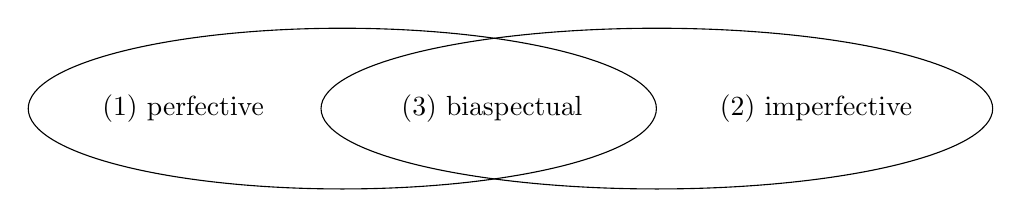
\begin{tikzpicture}[every fit/.style={ellipse,draw,inner xsep=-10pt,inner ysep=\baselineskip}]
\node at (0,0) (perfective) {(1) perfective};
\node [right=1.5cm of perfective] (biaspectual) {(3) biaspectual};
\node [right=1.5cm of biaspectual] (imperfective) {(2) imperfective};
\node [fit = (perfective) (biaspectual)] {};
\node [fit = (imperfective) (biaspectual)] {};
\end{tikzpicture}
\end{figure}

The new positive test for perfectivity proposed in \citet{ZinovaFilip:13} capitalizes on the notion of the \textit{Narration relation}, defined by \citet{Lascarides:93} as follows:

\begin{quote}
\textit{Narration($\alpha,\beta$)}: The event described in $\beta$ is a consequence of (but not strictly speaking caused by) the event described in $\alpha$. If \textit{Narration ($\alpha,\beta$)} holds, and $\alpha$ and $\beta$ describe eventualities \textit{e$_1$} and \textit{e$_2$}, respectively, then \textit{e$_1$} occurs before \textit{e$_2$}.
\end{quote}

The \textit{Narration} relation can be illustrated by \ref{textnar}: 
\ex.\label{textnar} Max woke up. He opened the window. 

In English, it is natural to use telic verb phrases in non-progressive tense in the \textit{Narration} relation. A parallel Russian example \ref{narrus} contains two perfective verbs. It is well-known  in the literature on aspect and discourse structure that the main line of a narrative is constituted by sequences of perfective verb forms which move narrative time forward \citep[for Russian, see in particular][]{Paducheva:96, Paducheva:04}.
\exg.\label{narrus}Maksim prosnulsja\textsuperscript{\PF}. On otkryl\textsuperscript{\PF} okno.\\
Maksim woke.up.\glb{pst.sg.m}.refl he open.\glb{pst.sg.m} window.\glb{sg.acc}\\
\trans `Maksim woke up. He opened the window.'

The property the test relies on is that if the Narration Relation holds and the second verb is perfective, the aspect of the first verb must be perfective as well. Example \ref{narrusbad} demonstrates that the combination of an imperfective and a perfective verb is uninterpretable. Under the most normal assumptions about how situations in the world take place, people do not open the windows while sleeping, nor is the event of opening a window normally interpreted as result or a continuation of the waking up event. Given that, the only possible relation between the two events (waking up and opening the window) is \textit{Narration}.
\exg.\label{narrusbad}$^{??}$Maksim prosypalsja\textsuperscript{\IPF}. On otkryl\textsuperscript{\PF} okno.\\
\hspaceThis{$^{??}$}Maksim woke.up.imp.\glb{pst.sg.m}.refl he open.\glb{pst.sg.m} window.\glb{sg.acc}\\
\trans\hspaceThis{$^{??}$}`Maksim was waking up. He opened the window.'\footnote{The English translation of this discourse seems to be much better than the Russian original. This effect is probably due to the different range of possible interpretations of the verbs \textit{prosypat'sja} `to wake up' and \textit{to wake up}. The Russian verb \textit{prosypat'sja} `to wake up' can only refer to the period before getting out of bed.}

\begin{table}
\caption{\label{table}Verbal aspect and the \textit{Narration} relation}
\begin{tabular}{llc}
\lsptoprule
\multicolumn{2}{c}{Verbal combination}& Acceptability judgment\\\midrule
perfective verb & \textit{i} `and' perfective verb~ & ok\hphantom{\textsuperscript{\textit{a}}}\\
imperfective verb & \textit{i} `and' perfective verb~ & ??\footnote{I use this sign to indicate a problem on the discourse level.}\\
biaspectual verb & \textit{i} `and' perfective verb~ & ok\hphantom{\textsuperscript{\textit{a}}}\\
\lspbottomrule
\end{tabular}
\end{table}

The idea of the test is summarized in Table~\ref{table}. \citet{ZinovaFilip:13} propose to use as test contexts sentences like \ref{test1} and \ref{test2}. The task is to enforce the Narration Relation  between the two clauses (see more details below). In this case if the verb in the second clause is perfective, the first verb must be perfective as well. Example~\ref{test1} is in the non-past, whereas \ref{test2} -- in the past tense. This shows that tense is not relevant for the purpose of the test. Note that this is not to deny that the Narration Relation may also hold in sequences with imperfective verbs only, as in \ref{ex:nar:imp}.
\ex.\label{test1}\ag.\label{test11}Ja s''em\textsuperscript{\PF} zavtrak i pojdu\textsuperscript{\PF} na rabotu.\\
I s.eat.\glb{pres.1.sg} breakfast and po.go.\glb{pres.1.sg} on work\\
\trans `I will finish my breakfast and go to work.'
\bg.\label{test12}$^{??}$Ja em\textsuperscript{\IPF} zavtrak i pojdu\textsuperscript{\PF} na rabotu.\\ 
\hspaceThis{$^{??}$}I eat\glb{.pres.1.sg} breakfast and po.go.\glb{pres.1.sg} to work\\

\ex.\label{test2}\ag.\label{test21}Ja s''el\textsuperscript{\PF} zavtrak i po\v{s}el\textsuperscript{\PF} na rabotu.\\
I s.eat.\glb{pst.sg.m} breakfast and po.go.\glb{pst.sg.m} on work\\
\trans `I finished my breakfast and went to work.'
\bg.\label{test22}$^{??}$Ja el\textsuperscript{\IPF} zavtrak i po\v{s}el\textsuperscript{\PF} na rabotu.\\
\hspaceThis{$^{??}$}I eat.\glb{pst.sg.m} breakfast and po.go.\glb{pst.sg.m} to work\\

\exg.\label{ex:nar:imp}U\v{z}e 8:00. Ja em\textsuperscript{\IPF} zavtrak i idu\textsuperscript{\IPF} na rabotu.\\
already 8:00. I eat.\glb{pres.1.sg} breakfast and go.\glb{pres.1.sg} to work\\
\trans `It is already 8:00. I eat breakfast and go to work.'

Examples \ref{test11} and \ref{test21} illustrate the first line of the table, \ref{test12} and \ref{test22} -- the second line of the table. \ref{test12} and \ref{test22} are not interpretable, because neither the Narration Relation nor any other coordinating relation, e.g., a Background Relation, can be construed. 

Examples \ref{biasp} illustrate the third line of the table above, which is crucial in case of biaspectual verbs. In a given context, \textit{kaznit'} `to execute' can behave either as a perfective or as an imperfective verb. Given that in the test context imperfective verbs are odd, biaspectual verbs pattern together with perfective verbs. Thus, the proposed test context allows us to distinguish between biaspectual and imperfective verbs. 
\ex.\label{biasp}\ag.Pala\v{c} kaznit prestupnika i pojd\"et\textsuperscript{\PF} domoj.\\
hangman execute.\glb{pres.3.sg} criminal and po.go.\glb{pres.3.sg} home\\
`The hangman will execute the criminal and will go home.'
\bg.Pala\v{c} kaznil prestupnika i po\v{s}el\textsuperscript{\PF} domoj.\\
hangman execute.\glb{pst.sg.m} criminal and po.go.\glb{pst.sg.m} home\\
`The hangman executed the criminal and went home.'

Now that the basic workings of the test are explained, let me address the precise conditions under which it works as a positive test for perfectivity. To enforce the \textit{Narration} relation, the following conditions are required to be met.
\begin{enumerate}
\item The main lexical verb in the second clause must have a temporal extent.
\item The event denoted by the main lexical verb in the second clause must not be caused or considered a continuation of the event denoted by the main lexical verb in the first clause.
\item The clauses must be conjoined using plain conjunction \textit{i} `and' without any temporal or modal (epistemic) adverbial.
\end{enumerate}
The conditions above reveal the workings of the test. When the clauses headed by two verbs, where the second one is perfective, are conjoined with \textit{i} `and' (condition 3), several coordinating discourse relations can be established between them. Conditions 1 and 2 ensure that such coordinating relations as Background or Cause are excluded. After this the only possible relation between the two clauses is Narration. If the Narration Relation  cannot be established, the discourse is infelicitous, as in \ref{test12} and \ref{test22}.

The reason for the first condition is that verbs denoting punctual events could be construed as describing events that are temporally located within the time span of the first event. In such a case, it is not the Narration (but the Background) Relation that holds between the two clauses, and thus the rule expressed in the last line of the table above (Table~\ref{table}) is not applicable, as illustrated by \ref{test5}. This condition is relevant if the test is applied in the past tense.
\exg.\label{test5}Ona igrala\textsuperscript{\IPF} v futbol i slomala\textsuperscript{\PF} nogu.\\
she play.\glb{pst.sg.f} in football and break.\glb{pst.sg.f} leg\\
\trans `While she was paying football, she broke her leg.'

\exg.\label{ex:cause}Ona xoro\v{s}o igrala\textsuperscript{\IPF} i zarabotala\textsuperscript{\PF} nagradu.\\
she well play.\glb{pst.sg.f} and za.work.\glb{pst.sg.f} reward\\
\trans `She was playing well and earned a reward.'

Examples like \ref{ex:cause} show the importance of the second condition: if the events denoted by the two main verbs are connected, the discourse relation is not one of Narration. According to \citet{Txurruka:03}, the natural language conjunction `and' marks a coordinating relation, which means is a relation of Narration, Background, Result, Continuation, Parallel or Contrast \citep{Asher:05}. To ensure a proper application of the test, one has to establish a context where the Narration relation is the only possible one between the two events. 

On the basis of the observation by \citet{Txurruka:03} that Narration is marked by \textit{then}, I propose to use the substitution of \textit{potom} `then' instead of \textit{i} `and' to check whether it is in fact Narration that connects the two coordinated clauses. If it is, then the meaning of the two sentences is (nearly) identical (compare \ref{test1} with \ref{breakfast:potom}). If it is not, the meaning changes significantly after such a substitution. To see this, compare \ref{test5} with \ref{football:potom} and \ref{ex:cause} with \ref{ex:cause:potom}: the sentences in \ref{football:potom} and \ref{ex:cause:potom} suggest that the second event is not caused or explained by the first one. These examples also illustrate why \textit{potom} `then' cannot be used for the purposes of the test directly: it establishes the Narration relation even in case of the different aspects of the main verbs in the two clauses.

\ex.\ag.\label{breakfast:potom}Ja s''em\textsuperscript{\PF} zavtrak, potom pojdu\textsuperscript{\PF} na rabotu.\\
I s.eat.\glb{pres.1.sg} breakfast then po.go.\glb{pres.1.sg} on work\\
\trans `I will finish my breakfast, then I will go to work.'
\bg.\label{football:potom}Ona igrala\textsuperscript{\IPF} v futbol, potom slomala\textsuperscript{\PF} nogu.\\
she play.\glb{pst.sg.f} in football then break.\glb{pst.sg.f} leg\\
\trans `She was playing football, then she broke her leg.'
\bg.\label{ex:cause:potom}Ona xoro\v{s}o igrala\textsuperscript{\IPF}, potom zarabotala\textsuperscript{\PF} nagradu.\\
she well play.\glb{pst.sg.f} then za.work.\glb{pst.sg.f} reward\\
\trans `She was playing well, then she earned a reward.'

\ex.\label{test3}\ag.\label{test31}Ja em\textsuperscript{\IPF} zavtrak. Pojdu\textsuperscript{\PF} na rabotu.\\ 
I eat.\glb{pres.1.sg} breakfast po.go.\glb{pres.1.sg} to work\\
\trans `I'm eating breakfast. I will go to work.'
\bg.\label{test32}$^?$Ja em\textsuperscript{\IPF} zavtrak i potom pojdu\textsuperscript{\PF} na rabotu.\\ 
I eat.\glb{pres.1.sg} breakfast and afterwards po.go.\glb{pres.1.sg} to work\\
\trans `I'm eating breakfast and will go to work afterwards.'
\bg.\label{test33}$^?$Ja em\textsuperscript{\IPF} zavtrak i objazatel’no pojdu\textsuperscript{\PF} na rabotu.\\
I eat.\glb{pres.1.sg} breakfast and necessarily po.go.\glb{pres.1.sg} to work\\
\trans `I'm eating breakfast and I of course will go to work.'
\bg.\label{test34}Ja em\textsuperscript{\IPF} zavtrak. Potom pojdu\textsuperscript{\PF} na rabotu.\\
I eat.\glb{pres.1.sg} breakfast afterwards po.go.\glb{pres.1.sg} to work\\
\trans `I'm eating breakfast. I will go to work afterwards.'

Examples under \ref{test3} demonstrate why the second condition is important: a sequence of two sentences without a conjunction or any explicit adverbial indicating their connection, as \ref{test31}, is acceptable in an appropriate context (for example if someone is asked about his plans; a pause will be present between the two sentences in such a case). Sentences \ref{test32} and \ref{test33} are at least much better than \ref{test12} and \ref{test22}. The last sentence, \ref{test34}, is completely natural. In these cases the Narration relation between the two clauses holds. In \ref{test32} and \ref{test34} it is explicit due to the presence of \textit{potom} `then' which, as mentioned above, is a marker of the Narration relation. As the idea of the test is to exclude all the coordinating relations (the coordinating requirement is imposed by \textit{i} `and', so it must be present) except for Narration and see whether this relation can be established given that the verb in the second clause is perfective, it is important to not include an explicit marker of this relation in the test context and, because that would force its application. Substituting  \textit{i} `and' with \textit{potom} `then' destroys the test context, as the Narration relation is enforced independently from the aspect of the verbs heading the clauses, as is evidenced by \ref{ex:potomcomma}.

\exg.\label{ex:potomcomma}Ja em\textsuperscript{\IPF} zavtrak, potom pojdu\textsuperscript{\PF} na rabotu.\\
I eat.\glb{pres.1.sg} breakfast afterwards po.go.\glb{pres.1.sg} to work\\
\trans `I'm eating breakfast, afterwards I will go to work.'

A similar situation is observed in the past tense: \ref{test41} is perfectly acceptable in a context in which the speaker remembers what he or she did on a given occasion, but only if there is a distinct pause between the two sentences; for \ref{test42}, there do not seem to be any clear judgments; and \ref{test43} is a plausible discourse.
\ex.\label{test4}\ag.\label{test41}Ja el\textsuperscript{\IPF} zavtrak. Po\v{s}el\textsuperscript{\PF} na rabotu.\\
I eat.\glb{pst.sg.m} breakfast. po.go.\glb{pst.sg.m} to work\\
\trans `I was eating breakfast. I went to work.'
\bg.\label{test42}$^?$Ja el\textsuperscript{\IPF} zavtrak i potom po\v{s}el\textsuperscript{\PF} na rabotu.\\
I eat.\glb{pst.sg.m} breakfast and afterwards po.go.\glb{pst.sg.m} to work\\
\trans `I was eating breakfast and went to work afterwards.'
\bg.\label{test43}Ja el\textsuperscript{\IPF} zavtrak. Potom po\v{s}el\textsuperscript{\PF} na rabotu.\\
I eat.\glb{pst.sg.m} breakfast. Afterwards po.go.\glb{pst.sg.m} to work\\
\trans `I was eating breakfast. I went to work afterwards.'

%\bg.\label{test52}Ona igrajet\textsuperscript{\IPF} v futbol i obyazatel'no slomajet\textsuperscript{\PF} nogu.\\
%She play.pres.3.sg in football and necesserely break.pres.3.sg leg\\
%She plays football and she will definitely break her leg once.
% The verb in the second clause is perfective and requires a time moment as an input. Such time moment, if not provided by an adverbial (condition 1), must be provided by the verb in the first clause, thus this verb must be perfective in order for the sentence to be felicitous.\\
Such examples should suffice to illustrate the basic intuition behind the test. The main idea of the test is the generalization given by \citet{Jespersen:24} that, if the verb is imperfective, it does not trigger narrative progression (in our case it is the verb in the first clause). Theoretically speaking, the relevant background for the workings of the test is best outlined in \citet{Altshuler:12}.
His account of the discourse properties of the Russian imperfective  relies on a multi-coordinate approach to aspect. He proposes interpretations for the \textsc{narr} operator and for the aspectual operators and explains why only perfective verbs are acceptable in \ref{ex:daniel:a} (ex. (73-a) in \citealt{Altshuler:12}), which is an example similar to our test context.

\ex.\label{ex:daniel}\ag.\label{ex:daniel:a}Lev ko mne \textsuperscript{\JudgeOK}priexal\textsuperscript{\PF} / {{$^{\#}$}priez\v{z}al\textsuperscript{\IPF}}\\
Lev to me {\hspaceThis{\textsuperscript{\JudgeOK}}pri.arrive.\glb{pst.3.sg}} / {{\textcolor{white} {$^{\#}$}}pri.arrive.imp.\glb{pst.3.sg}}\\
\bg.i srazu po\v{s}el\textsuperscript{\PF} ku\v{s}at'.\\
and right.away po.go.\glb{pst.3.sg} eat\\
\trans `Lev arrived at my place and went to eat right away.'\\
\hbox{}\hfill\hbox{(73-a) in \citet{Altshuler:12}}


%A good way of testing whether a verb is perfective is to identify contexts that only allow perfectives and contexts in which perfectives are excluded. Such contexts are those where a narration relation is established between the verb in question and a clearly perfective/imperfective verb, as in \ref{context1} and \ref{context2}:\\
%
%\ex.\label{context1} \ag. \label{context1:1}*Ja dopisyvaju\textsuperscript{\IPF} text i pojdu\textsuperscript{\PF} domoj.\\
%I do.write.imp\glb{prs.1.sg} text and go.\glb{pres.1.sg} home\\
%\bg. \label{context2:1}Ja dopisyvaju\textsuperscript{\IPF} text i idu\textsuperscript{\IPF} domoj.\\
%I do.write.imp\glb{prs.1.sg} text and go.\glb{pres.1.sg} home\\
%I plan to finish writing the text and go home.
%
%\ex.\label{context2} \ag. \label{context1:2}Ja dozapisyvaju\textsuperscript{\PF} disk i pojdu\textsuperscript{\PF} domoj.\\
%I do.za.write.imp\glb{prs.1.sg} CD and go.\glb{pres.1.sg} home\\
%I will finish recording the CD and go home.
%\bg. \label{context2:2}Ja dozapisyvaju\textsuperscript{\IPF} disk i idu\textsuperscript{\IPF} domoj.\\
%I do.za.write.imp\glb{prs.1.sg} and go.\glb{pres.1.sg} home\\
%I plan to finish recording the CD and go home.

\subsection{Applying the test}\label{subsection:bi:apply}
Now let us apply the test to the verbs \textit{dopisyvat'} `to finish/be finishing writing' and \textit{dozapisyvat'} `to finish/be finishing recording'. According to the syntactic theories, one aspect is always assigned to both verbs: either perfective \citep{Ramchand:04, Romanova:04, Svenonius:04b} or imperfective \citep{Tatevosov:07, Tatevosov:09}. However, as examples \ref{context1} and \ref{context2} show, these two verbs pattern differently with respect to the narration relation test. If the verb \textit{dopisyvat'} `to finish/be finishing writing' is inserted in the test context in the non-past tense, as in \ref{context1:1}, or in the past tense, as in \ref{context1:2}, both sentences are infelicitous. When the same contexts are populated with the verb \textit{dozapisyvat'} `to finish/be finishing recording', both resulting sentences are non-problematic.
\ex.\label{context1} \ag. \label{context1:1}$^{??}$Ja dopisyvaju tekst i pojdu\textsuperscript{\PF} domoj.\\
{\hspaceThis{$^{??}$}}I do.write.imp.\glb{pres.1sg} text and po.go.\glb{pres.1.sg} home\\
\bg. \label{context2:1}Ja dozapisyvaju disk i pojdu\textsuperscript{\PF} domoj.\\
I do.za.write.imp.\glb{pres.1.sg} CD and po.go.\glb{pres.1.sg} home\\
\trans `I will finish recording the CD and go home.'

\ex.\label{context2} \ag. \label{context1:2}$^{??}$Ja dopisyval text i po\v{s}el\textsuperscript{\PF} domoj.\\
{\hspaceThis{$^{??}$}}I do.write.imp.\glb{pst.sg.m} tekst and po.go.\glb{pst.sg.m} home\\
\bg. \label{context2:2}Ja dozapisyval disk i po\v{s}el\textsuperscript{\PF} domoj.\\
I do.za.write.imp.\glb{pst.sg.m} CD and go.\glb{pst.sg.m} home\\
\trans `I finished recording the CD and went home.'

Examples \ref{context3:1} and \ref{context3:2} show that the same results as for \textit{dozapisyvat'} are obtained for other verbs formed following the same pattern for biaspectual verbs \ref{form:do}. A good example is the verb \textit{dovy\v{s}ivat'} `to finish embroidering'. Notice that a verb with the same root but without the inner prefix \Prefix{vy-}, namely, \textit{do\v{s}ivat'}, `to finish/be finishing sewing', is not acceptable in the test context, as shown by examples \ref{context3:3} and \ref{context3:4}.
\ex.\label{context3}\ag.\label{context3:3}$^{??}$Ja do\v{s}ivala platje i podarila\textsuperscript{\PF} ego sestre.\\
{\hspaceThis{$^{??}$}}I do.sew.imp.\glb{pst.sg.f} dress and po.present.\glb{pst.sg.f} it sister\\
$^{??}$`I was finishing sewing this dress and I presented it to my sister.'
\bg.\label{context3:1}Ja dovy\v{s}ivala kartinu i povesila\textsuperscript{\PF} e\"e.\\
I do.embroid.imp.\glb{pst.sg.f} picture and po.hang.\glb{pst.sg.f} it\\
\trans `I finished embroidering the picture and hung it (on the wall).'

\ex.\label{context31}\ag.\label{context3:4}$^{??}$Ja do\v{s}ivaju platje i podarju\textsuperscript{\PF} ego sestre.\\
{\hspaceThis{$^{??}$}}I do.sew.imp.\glb{pres.1.sg} dress and po.present.\glb{pres.1.sg} it sister\\
$^{??}$`I am finishing sewing this dress and I will present it to my sister.'
\bg.\label{context3:2}Ja dovy\v{s}ivala kartinu i povesila\textsuperscript{\PF} e\"e.\\
I do.embroid.imp.\glb{pst.sg.f} picture and po.hang.\glb{pst.sg.f} it\\
\trans `I finished embroidering the picture and hung it (on the wall).'

To summarize, I have shown that the verbs formed according to the pattern in \ref{form:do}, e.g., \textit{dozapisyvat'} `to finish/be finishing recording', behave like verbs that are traditionally considered biaspectual (e.g., \textit{kaznit'} `to execute') and are intractable in the syntactic approaches.

% Chapter 3

\section{Derivational graph}\label{section:graph}
\subsection{Introduction}
As we have seen in the previous section, the existing approaches to Russian prefixation do not account for the full range of prefixed verbs data. Moreover, they often do not agree on the data or some important datapoint is missing or disregarded. This section is dedicated to the description of a structure that allows to reach an agreement on the prefixation data and easily check the proposed generalizations, if a database, organized according to the definition provided here, is implemented. Material presented in this section is partially covered in \citet{ZinovaFilip:14b}.

In the last part of this section, \sectref{subsection:predict}, I will show how the aspect of the verb can be easily predicted if we have the derivational graph, which is proposed here, at hand. In most cases such prediction is possible for a verb that is stored in the graph node exclusively on the basis of the information about the incoming edges. The cases where additional information (such as the aspect of the verb in the parent node) may be needed are discussed in Section~\ref{section:new:perfectivity}.

\subsection{Definitions}\label{section:chains:definition}
As we have seen in the previous chapter, some prefixed verbs can be derived in various ways. I propose to observe these possibilities carefully before excluding some of them that, at first glance, do not fit neatly into the common model of verbal prefixation.

The notion of a ``derivational chain'' used here is inspired by \citet{Karcevski:27} who proposed that ``[l]a valeur aspective d'un verbe d\'{e}pend de la place qu'il occupe dans la cha\^{i}ne de la d\'{e}rivation d\'{e}verbative'' [the aspectual value of a verb depends on its place in the chain of verbal derivation].

In the spirit of \citet{Karcevski:27}, the basic idea I pursue here is to infer the aspectual value (perfective or imperfective) of a given verb form from the derivational chain,\footnote{In \citet{ZinovaFilip:14b} we call it \textit{derivational history}.} rather than from the pure syntactic structure, as it is done in contemporary syntactic analyses. I also want to put forward the idea that the derivational chain does not have to be unique for a given verb. To formalize \citeauthor{Karcevski:27}'s (\citeyear{Karcevski:27}) suggestions about what constitutes a derivational chain, I propose the following definition:

\begin{definition}\label{def:history}
A verb V$_2$ is derived from a verb V$_1$ if and only if
\begin{enumerate}[noitemsep,nosep]
\item both V$_1$ and V$_2$ are attested in the language;
\item there is a morphological operation (the extensive list of such operations is provided by \citealt{Shvedova:82}) such that it takes as an input the verb V$_1$ and provides as an output the verb V$_2$;
\item the meaning of V$_2$ can be monotonically (possibly not entirely compositionally) derived from the meaning of V$_1$;
\item there is no other verb V$_3$ such that V$_3$ is derived from V$_1$ and V$_2$ is derived from V$_3$.
\end{enumerate}
\end{definition}

To illustrate the above definition of a derivational chain, let us consider the verbs \textit{kupit'\textsuperscript{\PF}} and \textit{pokupat'\textsuperscript{\IPF}} `to buy'. There are three possible ways in which these verbs might be related, shown in \ref{chain:pokupat}.

\ex.\label{chain:pokupat}\ag.\label{chain:pokupat1}kup-i-t'\textsuperscript{\PF} $\rightarrow$ *po-kup-i-t' $\rightarrow$ po-kup-a-t'\textsuperscript{\IPF}\\	
{to buy} $\rightarrow$ $\cdots$ $\rightarrow$ {to buy/to be buying}\\
\bg.\label{chain:pokupat2}kup-i-t'\textsuperscript{\PF} $\rightarrow$ po-kup-a-t'\textsuperscript{\IPF}\\
{to buy} $\rightarrow$ {to buy/to be buying}\\
\bg.\label{chain:pokupat3}kup-i-t'\textsuperscript{\PF} *$\rightarrow$ kup-a-t'\textsuperscript{\IPF} *$\rightarrow$ po-kup-a-t'\textsuperscript{\IPF}\\
{to buy} *$\rightarrow$ {to bathe} *$\rightarrow$ {to buy/to be buying}\\

The derivation in \ref{chain:pokupat1} is excluded, because *\textit{pokupit'} does not exist (violation of the first condition). The derivation in \ref{chain:pokupat2} is fine with respect to the first and the second conditions, so what we have to check for is the third condition. I.e., that there is no other verb such that it is derived from \textit{kupit'}\textsuperscript{\PF} `to buy'.  A candidate verb, formally speaking, would be \textit{kupat'\textsuperscript{\IPF}}, but it has an unrelated meaning `to bathe someone' (violation of the third condition). This also means that \ref{chain:pokupat3} cannot be considered to constitute a derivational chain.  

As we have just seen, the second chain, \ref{chain:pokupat2}, is a valid derivational chain, according to the three conditions above. However, it includes simultaneous (happening at one derivational step) attachment of two morphemes (the prefix \Prefix{po-} and the suffix \textit{-a-}). In this work I will not deal with such derivations that include a simultaneous addition of two or more morphemes (including cases of prefixation accompanied by the addition of the postfix) or discontinuous morphemes. I will limit myself to providing a computational account of verbal derivational morphology only for derivations that include an attachment of a single morpheme at each derivational step.

To provide an extension to the example~\ref{chain:pokupat}, let us also consider the candidate derivational chains for the verb \textit{napokupat'} `to buy a lot', presented in \ref{ex:napokupat}. The first candidate chain, \ref{ex:napokupat1}, demonstrates a violation of the third condition: there exists another verb (\textit{pokupat'} `to buy/be buying') such that it is derived from the verb \textit{kupit'} `to buy' and serves as a derivational base for obtaining the verb \textit{napokupat'} `to buy a lot'. So, despite the fact that the verb \textit{napokupat'} `to buy a lot' is (indirectly) derived from the verb \textit{kupit'} `to buy', the derivation in \ref{ex:napokupat1} is not a valid derivational chain. On the other hand, the chain in \ref{ex:napokupat2} is a derivational chain, according to the definition above, although only the second step of it will receive an analysis in this work. 

\ex.\label{ex:napokupat}\ag.\label{ex:napokupat1}kup-i-t'\textsuperscript{\PF} $\rightarrow$ na-po-kup-a-t'\textsuperscript{\PF}\\	
{to buy} $\rightarrow$ {to buy a lot}\\
\bg.\label{ex:napokupat2}kup-i-t'\textsuperscript{\PF} $\rightarrow$ po-kup-a-t'\textsuperscript{\IPF} $\rightarrow$ na-po-kup-a-t'\textsuperscript{\PF}\\
{to buy} $\rightarrow$ {to buy/to be buying} $\rightarrow$ {to buy a lot}\\

There is also another way to represent and store the information carried by the derivational chains, that is useful for computational purposes: a graph. Let us consider the following directed graph $D$: 
\begin{definition}\label{def:chain}
$D = (V,A)$, where V is a set of nodes labeled with verbs that are attested in the language and A is a set of ordered pairs of nodes. $\forall x,y \in V, (x,y) \in A$ iff  the verb that labels the node y can be derived from the verb that labels the node x (according to the \defref{def:history}).
\end{definition}

In what follows, I will call such graph $D$ a \textit{derivational graph.} Paths in this graph are derivational chains that are defined by \defref{def:history}. The number of connected components of the graph $D$ equals the number of verbal stems in the object language.

There exists a graph that is similar to the derivational graph described here. It represents derivational relations between Russian verbs and is a part of the OSLIN database\footnote{Open Source Lexical Information Network, available online at \url{http://ru.oslin.org/index.php?action=aspect}}, described in \cite{Borik:12}. The problem with this graph is that it is far from being complete, as the lexical items included are taken from dictionaries and, as we have already discussed, this covers a relatively small amount of prefixed verbs and almost none of the multiply prefixed verbs.

Let me also mention another database of Russian prefixed verbs\footnote{Available at \url{http://emptyprefixes.uit.no/}} provided by the CLEAR (Cognitive Linguistics: Empirical Approaches to Russian) group at the University of Troms{\o}. According to the description on the website, ``[t]his database contains information on 1,981 imperfective verbs in Russian that form aspectual pairs via prefixation'', aggregating entries from \citet{MAS}, \citet{Ozegov:01},  and \citet{Cubberly:82} that were approved by a panel of native speakers. This database, however, was constructed for the purpose of exploring the `empty' prefixes and thus is not a full derivational graph as it contains only verbs that form aspectual pairs (imperfective and perfective verbs with the same lexical meaning) via prefixation.

\subsection{Motivation}\label{section:chains:motivation}
Let me provide some motivation for the decisions made with respect to the (non) inclusion of the certain types of potential edges in the graph. The notion of a derivation graph can be understood in different ways. For the broader picture, one may want to have a full graph with all the possible connections. Such a graph will include edges connecting the nodes occupied by the verbs that are possibly semantically related but the relation is not evident for a native speaker (removing the third condition). Another option is a graph with all the connections as long as the verbs are semantically connected. If no restriction on the complexity and the direction of morphological transitions is imposed, forms that are not directly derived from each other will be connected, and the resulting structure will be a collection of ``nests'', not ``chains'' (removing the fourth condition). Such a structure, for example, is discussed in \citealt{Janda:10}. A more restricted graph can also be useful: for example, a graph where only the most transparent relations are marked (those where semantic transitions are compositional). 

Another graph is extracted from the dictionary data by \citet{Janda:07a} for her analysis of the structure of aspectual clusters (for a restricted list of verbs). For each source verb, \citeauthor{Janda:07a} lists not all the derived verbs but only one or two for each of the categories she distinguishes (Natural, Specialized, Complex Act, and Single Act Perfectives), thus reducing the complexity of the graph. In addition, the graph can be either directed or non-directed. 
 
The graph I propose to use is one with ``chain'' structures, which means that only direct connections are present and the nodes that can be reached through the transitive relations are not additionally directly connected. The second important point is that these chains will later be used to learn the rules of aspectual changes that happen at one derivational step. That is why it is good to include more relations, even those with non-compositional semantic steps. On the other hand, it does not make sense to include those transitions where the semantic relation between the verbs is not transparent at all: as this is not a regular process, such verbs are listed in the dictionaries and do not allow for generalizations. 

I have decided to include also the derivations with simultaneous attachment of multiple affixes. They are not analysed here, but among such derivations there are cases that must be taken into consideration in future work. For instance, it is claimed that some prefixes are attached simultaneously with postfixes. An example of such prefix is the cumulative \Prefix{na-}: if it is attached to the verb \textit{jest'} `to eat', two verbs can be derived: \textit{najest'sja} `to eat until becoming full' and \textit{najest'} `to gain fat in some part of the body as the result of eating' (colloquial). The semantics of the first verb cannot be  monotonically derived from the semantics of the second one, as the component of gaining fat would have to be absent in the derived verb (\ref{ex:najestsja1} is not a derivational chain). So we have to accept that the verb \textit{najest'sja} `to eat until becoming full' is derived directly from the verb \textit{jest'} `to eat' by simultaneous attachment of the prefix and the postfix, as illustrated by the chain \ref{ex:najestsja2}. Such verbs are not studied in this work, so I propose to include them in the derivational graph, but set them aside for the moment.
 
 \ex.\label{ex:najestsja}\ag.\label{ex:najestsja1}es-t'\textsuperscript{\IPF} $\rightarrow$ na-es-t'\textsuperscript{\PF} *$\rightarrow$ na-es-t'-sja\textsuperscript{\PF}\\	
{to eat} $\rightarrow$ {to gain fat} *$\rightarrow$ {to eat until becoming full}\\
\bg.\label{ex:najestsja2}es-t'\textsuperscript{\PF} $\rightarrow$ na-es-t'-sja\textsuperscript{\PF}\\
{to eat} $\rightarrow$ {to eat until becoming full}\\

The derivational graph, built in accordance with \defref{def:chain}, would be a perfect starting point for the investigation of the individual prefixes, as one could use derivational chains for making generalizations. For example, it would be easy to check whether a certain prefix allows a subsequent imperfectivization or can be attached on top of the other prefix: would only have to check the properties of the verbs that are connected with the edges labeled with the prefix in question in the derivational graph. 

Consider the verb \textit{pisat'} `to write' and the verb \textit{dopisyvat'} `to finish writing'. There is only one possible path from the verb \textit{pisat'} `to write' to the verb \textit{dopisyvat'} `to finish writing' in the derivational graph fragment illustrated by \figref{tree:dopisyvat}. This path is written as a derivational chain under \ref{deriv1-1}. Although the nodes for another way, shown in \ref{deriv1-2}, are present in the derivational graph, one of the edges (between the verb \textit{pisyvat'} `to write occasionally' and the verb \textit{dopisyvat'} `to finish/be finishing writing') is missing because of the semantic restriction (third condition in \defref{def:history}).

\ex.\label{deriv1} \ag.\label{deriv1-1}pisat'\textsuperscript{\IPF} $\rightarrow$ dopisat'\textsuperscript{\PF} $\rightarrow$ dopisyvat'\textsuperscript{\IPF}\\
{to write} $\rightarrow$ {to finish writing} $\rightarrow$ {to finish/be finishing writing}\\
\bg.\label{deriv1-2}pisat'\textsuperscript{\IPF} $\rightarrow$ pisyvat'\textsuperscript{\IPF} $\nrightarrow$ dopisyvat'\\
{to write} $\rightarrow$ {to write occasionally} $\rightarrow$ {to finish/be finishing writing}\\

\begin{figure}
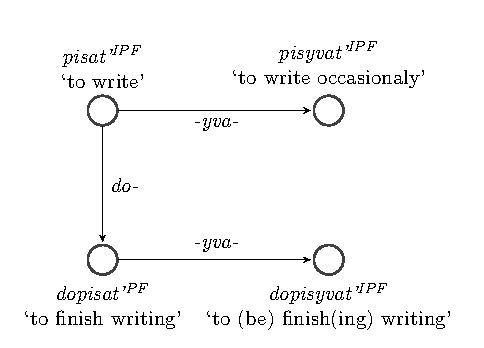
\includegraphics{graphPisat.pdf}
\caption{A fragment of the derivational graph: \textit{pisat'} `to write'\label{tree:dopisyvat}}
\end{figure}

The fragment of the derivational graph, presented on \figref{tree:dopisyvat}, provides evidence for the hypothesis that, if a verb contains both the prefix \Prefix{do-} and the imperfective suffix, it is imperfective. However, this hypothesis is quickly rejected on the basis of the other part of the graph: if one searches through the paths from the verb \textit{pisat'} `to write' to the verb \textit{dozapisyvat'} `to finish/be finishing writing down/recording', one finds two different derivational chains in the derivational graph, as shown in \figref{tree:dozapisyvat}. The first derivational chain, linearised in \ref{deriv:dozapisyvat1}, provides evidence against the proposed hypothesis, as the verb at the end of this chain is perfective and contains both the imperfective suffix and the prefix \Prefix{do-}. 

\ex.\label{deriv:dozapisyvat}\ag.\label{deriv:dozapisyvat1}pisat'\textsuperscript{\IPF} $\rightarrow$ zapisat'\textsuperscript{\PF} $\rightarrow$ zapisyvat'\textsuperscript{\IPF} $\rightarrow$ dozapisyvat'\textsuperscript{\PF}\\
{to write} $\rightarrow$ {to record} $\rightarrow$ {to (be) record(ing)} $\rightarrow$ {to finish recording}\\
\bg.\label{deriv:dozapisyvat2}pisat'\textsuperscript{\IPF} $\rightarrow$ zapisat'\textsuperscript{\PF} $\rightarrow$ dozapisat'\textsuperscript{\PF} $\rightarrow$ dozapisyvat'\textsuperscript{\IPF}\\
{to write} $\rightarrow$ {to record} $\rightarrow$ {to finish recording} $\rightarrow$ {to (be) finish(ing) recording}\\				

\begin{figure}
\begin{center}
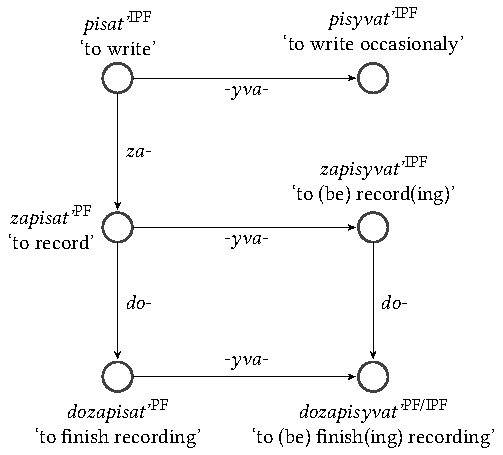
\includegraphics[scale=1]{graphDozapisyvat.pdf}
\caption{A fragment of the derivational graph: \textit{pisat'} `to write' and \textit{dozapisyvat'} `to (be) finish(ing) recording'\label{tree:dozapisyvat}}
\end{center}
\end{figure}			

The example above is just one illustration of how a derivational graph defined by \defref{def:chain} can be used to check possible generalizations about the properties of Russian prefixed verbs. Such a graph, however, does not exist in the form of a human-created resource\footnote{The graph itself exists by definition, so what I mean here is some resource that stores this graph and allows to extract information from it.} and some researchers doubt even the possibility of writing it down in an overt form. For example, \citet[625]{Janda:07a} claims that ``exhaustive listings of verbs would be unwieldy, and, given the ad-hoc open-class nature of Specialized Perfectives and Complex Acts, such lists could never be definitive''. \citet[626]{Janda:07a} also regards most of the verbs that are not listed in the dictionaries and constructed spontaneously by the speakers not to be a core part of the verbal cluster.

I do not agree with the claim about the marginal status of such verbs and consider them one of the core components of the Russian verbal system. Moreover, I claim that there is a way to construct a derivational graph defined above. To do this, I propose to take the following approach: I base the generalizations in this and the following chapters on the data about parts of this graph that are built using introspection and corpora/search engine data. Afterwards, in Chapters~\ref{Chapter7} and \ref{Chapter8}, I propose a formal account that is capable of predicting which vertices and edges, apart from those already included on the basis of dictionary data, should be added to the derivational graph (at the moment only with respect to the five prefixes I analyse in this work). I also check these predictions at least partially against corpora and search engine data. The output of the computational system I propose can later be used to build a larger version of the derivational graph. An implemented database that is constructed on the basis of the dictionary data, such as OSLIN, can serve as a starting point for the proposed construction.

\subsection{Predicting the aspect of the derived verb}\label{subsection:predict}
As discussed in Section~\ref{subsection:bi:predictions}, the property that drives the analysis proposed here and is implicitly rejected by the syntactic theories of Russian prefixation is that a given verb does not need to be associated with a unique derivational chain. For example, the biaspectual verb \textit{dozapisyvat'} `to (be) finish(ing) recording/writing down' appears as the last node of two derivational chains given in \ref{deriv:dozapisyvat}, where one of them motivates the perfective aspect of the whole verb \ref{deriv:dozapisyvat1}, while the other motivates the imperfective aspect of the same verb \ref{deriv:dozapisyvat2}.

For a verb to have two derivational chains implies that it may be ambiguous with respect to grammatical aspect: each derivational chain yields exactly one grammatical aspect for the derived verb, either perfective or imperfective. The context then presumably selects one of the derivational chains, and consequently, either the perfective or imperfective aspect of the verb, contrary to the syntactic approaches (in their existing form), which can only provide one derivational chain for any given complex verb form due to formal restrictions on the positions of different affixes.

This is desirable given that, judging from the data, the verb \textit{dozapisyvat'} `to (be) finish(ing) recording/writing down' is genuinely ambiguous with respect to the perfective/imperfective distinction, and it is the context that enforces one or the other grammatical aspect assignment. Note that the two derivational chains in \ref{deriv:dozapisyvat1} and \ref{deriv:dozapisyvat2}, discussed above, straightforwardly follow from the two general patterns that are widely accepted as governing the formation of Russian verbs, although there are also some exceptions to them that will be discussed in Section~\ref{section:new:perfectivity}:

\begin{enumerate}
\item the output of a prefixation is perfective;   
\item adding the imperfective suffix to a verb yields an imperfective verb. 
\end{enumerate}

The root verb in \ref{deriv:dozapisyvat1} and \ref{deriv:dozapisyvat2} is the primary imperfective verb \textit{pisat'} `to write/to be writing'. Adding the prefix \textit{za}- to it yields a perfective verb, in compliance with (1), and the attachment of the imperfective suffix -\textit{yva}- yields a secondary imperfective verb, following (2). This verb in turn serves as the basis for the prefixation with the completive prefix \Prefix{do-}. The result is the perfective verb \textit{dozapisyvat'} `to finish recording/writing down', in compliance with (1).  In \ref{deriv:dozapisyvat2}, the second and the third steps are reversed, leading to the imperfective category assignment to the derived verb \textit{dozapisyvat'} `to finish/be finishing recording/writing down'.

Let me explain why the approach outlined here leads to different predictions than the syntactic accounts despite the fact that in both cases it is the final step of the derivation that determines the aspect of the whole complex verb. The crucial assumption of the syntactic approaches to prefixation in Russian is that each prefix (with fixed interpretation) occupies a particular position in the syntactic tree. From this it follows that structural properties of the verbs that have the same outermost prefixes are always the same. For example, the verbs that we have just considered, \textit{dopisyvat'}\textsuperscript{\IPF} `to (be) finish(ing) writing' and \textit{dozapisyvat'}\textsuperscript{\IPF\slash\PF} `to finish/be finishing recording/writing down', are either both perfective or both imperfective on any existing syntactic prefixation account, as they contain the same outermost prefix \Prefix{do-} and its position in the tree determines the aspect of the whole verb. On the account advocated here, there is an evident difference between these verbs, as the order of the derivational steps is determined based on all possible derivational chains that are constructed in compliance with \defref{def:history}. While the verb \textit{dozapisyvat'}\textsuperscript{\IPF\slash\PF} `to (be) finish(ing) writing down/recording' has two derivational chains, as has been shown by \ref{deriv:dozapisyvat1} and \ref{deriv:dozapisyvat2}, which motivates its biaspectual nature, the imperfective verb \textit{dopisyvat'}\textsuperscript{\IPF} `to finish/be finishing writing' has only one, as has been shown by \ref{deriv1}, so it can be only assigned the imperfective aspect.

Another example, already mentioned in Section~\ref{subsection:bi:apply}, is the verb \textit{dovy\v{s}ivat'} `to finish embroidering'. It contains the same type of affixes as the verb \textit{dozapisyvat'} `to finish recording/writing down'. Namely, a completive prefix \Prefix{do-}, one more prefix commonly characterized as a lexical prefix, and the imperfective suffix. The verbs \textit{dovy\v{s}ivat'} `to finish embroidering' and \textit{dozapisyvat'} `to finish recording/writing down' are morphologically alike and thus there is no structural difference between them on any existing syntactic account of Russian verbal prefixation, as the structure of the verb and the order of the affix attachment is determined only on the basis of the syntactic properties of the affixes (with fixed interpretation).
 
It turns out that these verbs are clearly different for most native speakers: while the perfective uses of the verb \textit{dozapisyvat'} `to finish recording/writing down' may be judged odd by some speakers (as claimed by Sergei Tatevosov, personal communication\footnote{Note that such behaviour can be explained on the account proposed here by assuming that these speakers use a stronger version of a general pragmatic principle that is used to account for the non-existence of a range of verbs (more information in Chapters~\ref{Chapter5} and~\ref{Chapter6}). This principle says that a more complex morphological form cannot be used to express the same meaning that a less marked form has. As a default, the domain of available alternatives is restricted to the verbs belonging to one derivational chain (where the complexity is directly connected to the place in the chain). In the stronger version, however, one can widen the domain to all the chains that start from the same source node. This modification will allow to account for the variation in the acceptability of various verbs.}), all the native speakers that I have consulted with agree that the verb \textit{dovy\v{s}ivat'} `to finish embroidering' can be used as a perfective verb. Moreover, most of these speakers do not accept \textit{dovy\v{s}ivat'} `to finish embroidering' as an imperfective verb. The same group of people rejects the existence of the verb $^?$\textit{dovy\v{s}it'}\textsuperscript{\PF} `to finish embroidering'. This behavior is easily explained by means of the relevant part of the derivational graph, presented on \figref{tree:dovyshivat}. For the group of speakers who reject the existence of the verb $^?$\textit{dovy\v{s}it'}\textsuperscript{\PF} `to finish embroidering', the derivation in \ref{deriv:dovyshivat2} is not available, as it requires the verb $^?$\textit{dovy\v{s}it'}\textsuperscript{\PF} `to finish embroidering' to be attested. Thus the verb \textit{dovy\v{s}ivat'} `to finish embroidering' cannot be assigned the imperfective aspect. On the other hand, at least some of the speakers that accept the verb $^?$\textit{dovy\v{s}it'}\textsuperscript{\PF} `to finish embroidering' also have access to the imperfective aspect of the verb \textit{dovy\v{s}ivat'} `to finish embroidering'.

\ex.\label{deriv:dovyshivat}\ag.\label{deriv:dovyshivat1}\v{s}it'\textsuperscript{\IPF} $\rightarrow$ vy-\v{s}it'\textsuperscript{\PF} $\rightarrow$ vy-\v{s}-iva-t'\textsuperscript{\IPF} $\rightarrow$ do-vy-\v{s}-iva-t'\textsuperscript{\PF}\\
{to sew} $\rightarrow$ {to embroider} $\rightarrow$ {to embroider/be embroidering} $\rightarrow$ {to finish embroidering}\\
\bg.\label{deriv:dovyshivat2}\v{s}it'\textsuperscript{\IPF} $\rightarrow$ vy-\v{s}it'\textsuperscript{\PF} $\rightarrow$ do-vy-\v{s}it'\textsuperscript{\PF} $\rightarrow$ do-vy-\v{s}-iva-t'\textsuperscript{\IPF}\\
{to sew} $\rightarrow$ {to embroider} $\rightarrow$ {to finish embroidering} $\rightarrow$ {to finish/be finishing embroidering}\\

\begin{figure}
\begin{center}
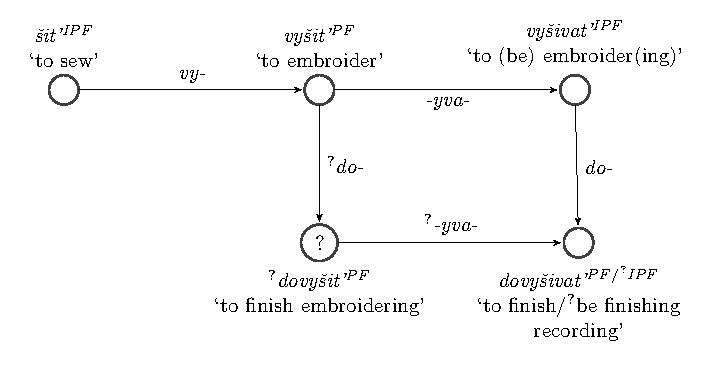
\includegraphics[scale=1]{graphDovyshivat.pdf}
\caption{A fragment of the derivational graph: \textit{\v{s}it'} `to sew' and \textit{dovy\v{s}ivat'} `to finish embroidering'\label{tree:dovyshivat}}
\end{center}
\end{figure}		

I would like to also point out another question that naturally arises in connection with the possible paths in the derivational graph. One may ask whether there are prefixes that can be considered perfectivity markers. The first step towards answering this question would be to look for a prefix such that whenever a verb contains it, there are no outgoing edges from the node corresponding to this verb in the derivational graph. Although this is a reformulation of one of the classical characteristics of the superlexical prefixes,\footnote{See, e.g. \citet{Ramchand:04}, \citet{Svenonius:04a}, and \citet{Romanova:06}, who assume that superlexical prefixes occupy the highest position in the verbal structure.} \citet{Tatevosov:07, Tatevosov:09} provides numerous counterexamples to such a constraint. In the account proposed in \citealt{Tatevosov:09}, the main constraints on the attachment of the superlexical prefixes are formulated in different terms: they must be attached either before the imperfective suffix or to a formally imperfective verb. Only the distributive prefix \textit{po}- that, according to \citet{Tatevosov:09}, occupies the left periphery of the verb, is then a prefix of such a type that the verb that contains it is necessarily perfective and no other morpheme can be attached higher than it. I will further investigate the ability of the individual prefixes discussed here to constitute a part of an imperfective verb in Chapter~\ref{Chapter5}.\footnote{Note that even if we find such prefixes that can be encountered only on the last derivational step, they are not necessarily perfectivity markers, as there may be other reasons (e.g. semantic, pragmatic, phonological) why further derivational steps are not possible.}

\section{Prefixation and perfectivity}\label{section:new:perfectivity}

\subsection{Introduction}
It is generally assumed in Russian morphology that, if the last step of the verbal derivation is prefixation, the verb comes out perfective. This fact does not depend on the point where the perfectivity comes in: in both aspect-low \citep[][among others]{Verkuyl:95, Pinon:01, Ramchand:04} and aspect-high \citep{Paslawska:03, Gronn:10, Tatevosov:11} theories, prefixes carry some property that either immediately or later leads to the perfective aspect of the verb. In this section we will discuss cases that seem to provide exceptions to this pattern.

In the first part, Section~\ref{subsection:perf:borrowed}, we will look at the prefixation of borrowed biaspectual verbs with native prefixes. Then, in Section~\ref{subsection:perf:imperf}, we will examine what happens if an imperfective verb derived from a borrowed root gets prefixed. Next, in Section~\ref{subsection:perf:native}, we will discuss the case of native biaspectual verbs and their prefixation. The discussion will be followed by some information on borrowed prefixes, as they do not affect the aspect of the verb they are attached to (Section~\ref{subsection:perf:prefixes}). We will then close with considering the problem of motion verbs that are often said to resist perfectivization when prefixed (Section~\ref{subsection:perf:motion}, also published as \citealt{ZinovaOsswald:paper}).

\subsection{Prefixation of borrowed biaspectual verbs}\label{subsection:perf:borrowed}
Consider the verbs \textit{perezapisat}'\textsuperscript{\PF} `to rerecord' and \textit{zapisyvat'}\textsuperscript{\IPF} `to  record/be recording'. Both verbs are attested and commonly used by native speakers. Intuitively, the verb \textit{perezapisyvat'} `to rerecord/be rerecording' can be formed from either of them: one can add the imperfective suffix to the verb \textit{perezapisat}'\textsuperscript{\PF} `to rerecord' or the repetitive prefix \Prefix{pere-} to the verb \textit{zapisyvat'}\textsuperscript{\IPF} `to (be) record(ing)'. This is schematically shown in \ref{schema:perezapisyvat'}.

\ex.\label{schema:perezapisyvat'}\ag.\label{schema:perezapisyvat'1}pisat'\textsuperscript{\IPF} {$\rightarrow$} zapisat'\textsuperscript{\PF} {$\rightarrow$} perezapisat'\textsuperscript{\PF} {$\rightarrow$} perezapisyvat'\textsuperscript{\IPF} \\
{`to write'} {} {`to record'} {} {`to rerecord'} {} {`to rerecord/be rerecording'}\\
\bg.\label{schema:perezapisyvat'2}pisat'\textsuperscript{\IPF} {$\rightarrow$} zapisat'\textsuperscript{\PF} {$\rightarrow$} zapisyvat'\textsuperscript{\IPF} {$\rightarrow$} perezapisyvat'\textsuperscript{\IPF} \\
{`to write'} {} {`to record'} {} {`to record/be recording'} {} {`to rerecord/be rerecording'}\\

The derivational chain in \ref{schema:perezapisyvat'2} is excluded under all accounts for verbal prefixation, since it violates the assumption that adding a prefix as a last derivational step makes the derived verb perfective. However, on the intuitive level, the derivation in \ref{schema:perezapisyvat'2} is acceptable. This leads to us to question the hypothesis of a uniform perfectivizing function of all the verbal prefixes in Russian. In order to address this question, we have to look at some derivations where there is no potential for switching the order of the derivational steps.

A case in point are borrowed biaspectual verbs. Consider the biaspectual verb \textit{kvalificirovat'} `to qualify/to classify'. It is formed with the native verbal suffix -\textit{irova}-, which instantiates one of the systematic patterns of formation of borrowed verbs. This verb can be prefixed with the repetitive prefix \Prefix{pere-}. The result of such a prefixation is the verb \textit{perekvalificirovat'} `to requalify/to recategorize', which is, in turn, also biaspectual.

In order to show that in this case prefixation does not lead to the perfective aspect of the verb, I have to prove two things: (1) that the verb \textit{perekvalificirovat'} `to requalify/to recategorize' is indeed biaspectual and (2) that there is no other way to derive the verb \textit{perekvalificirovat'} `to requalify/to recategorize' than by attaching the prefix \Prefix{pere-} to the verb \textit{kvalificirovat'} `to qualify/to classify'.

To show that the prefixed verb \textit{perekvalificirovat'} `to requalify/to reclassify' is  biaspectual, let me provide evidence of its usage both as a perfective and as an imperfective verb. Example \ref{ex:perekvalificirovat:perf} illustrates the usage of the verb \textit{perekvalificirovat'} `to requalify/to reclassify' in the perfective aspect and the constructed sentence \ref{ex:perekvalificirovat:perf2} shows that perfective aspect is available according to the test offered in Section~\ref{sec:tests:new}.

\ex.\ag.\label{ex:perekvalificirovat:perf}Krome togo, vynosja prigovor, sud'ja perekvalificiroval\textsuperscript{\PF} obvinenie i snizil s ``osobo krupnogo'' na ``krupnyj'' objem nefti, v xi\v{s}\v{c}enii kotoroj obvinjajutsja podsudimye.\\
apart this, vy.carry.\glb{part.pres} sentence.\glb{sg.acc} judge.\glb{sg.nom} pere.classify.\glb{pst.sg.m} accusation.\glb{sg.acc} and lower.\glb{pst.sg.m} from ``particularly large'' on ``large'' volume.\glb{sg.acc} oil.\glb{gen} in theft.\glb{sg.prep} which.\glb{f.sg.prp} accuse.\glb{pres.3.pl.}refl defendant.\glb{pl.nom}\\
\trans `Apart from this, when pronouncing the sentence, the judge reclassified the accusation, changing the amount of oil that the defendants are accused of stealing from ``particularly large'' into ``large''.'\\
\hbox{}\hfill\hbox{\url{http://www.vesti.ru}}
\bg.\label{ex:perekvalificirovat:perf2}Sud'ja perekvalificiroval\textsuperscript{\PF} delo i po\v{s}\"{e}l domoj.\\
judge.\glb{sg.nom} pere.classify.\glb{pst.sg.m} case.\glb{sg.acc} and po.go.\glb{pst.sg.m} home\\
\trans `The judge reclassified the case and went home.'

To show that the verb \textit{perekvalificirovat'} `to requalify/to reclassify' can also be used as an imperfective verb, I apply to it the four common tests that delimit imperfective verbs. It turns out that in an appropriate context the verb \textit{perekvalificirovat'} `to requalify/to reclassify' can have a progressive interpretation, as shown by example \ref{ex:qualify1}, it can be used as a complement of a phasal verb, as in \ref{ex:qualify2}, form periphrastic future, as in the sentence \ref{ex:qualify3}, and form a present participle, as in \ref{ex:qualify4}. 

\ex.\label{ex:qualify}\ag.\label{ex:qualify1}V dannyj moment on perekvalificiruet\textsuperscript{\IPF} svoju {``Armiju Maxdi''} v politi\v{c}eskoe dvi\v{z}enie.\\
in given moment he pere.qualify.\glb{pres.3.sg} his {``Armija Maxdi''} in political movement\\
\trans `Right now he is re-categorizing his ``Armija Maxdi'' into a political movement.'\hbox{}\hfill\hbox{\url{subscribe.ru}}
\bg.\label{ex:qualify2}Sej\v{c}as advokaty na\v{c}nut perekvalificirovat'\textsuperscript{\IPF} delo v politi\v{c}eskoje.\\
now advocates start.\glb{pres.3.pl} iter.qualify.\glb{inf} case in political\\
\trans `Now the advocates will start to re-classify this case as a political one.'\\\hbox{}\hfill\hbox{\url{pikabu.ru}}
\bg.\label{ex:qualify3}Policejskix budut perekvalificirovat'\textsuperscript{\IPF} v buxgalterov.\\	
policemen will.be pere.qualify\glb{.inf} in accountant.\glb{pl.acc}\\
\trans `Policemen will be re-trained and become accountants.'\hbox{}\hfill\hbox{\url{pikabu.ru}}
\bg.\label{ex:qualify4}Ne pozvoljaetsja smotret’ na perekvalificiruemye sdelki s pozicii togo, \v{c}to nalogoplatel’\v{s}\v{c}ik mog sdelat’ v tex uslovijax.\\
not allow look on pere.qualify.\glb{part.pres.pl.acc} deals from position that, that tax.payer can.\glb{pst.sg.m} s.do.\glb{inf} in that conditions\\
\trans `We cannot view the deals which are subject to reclassification on the basis of what a tax-payer would have done under the same circumstances.'\hbox{}\hfill\hbox{\url{www.aetc.ru}}

Now let us examine other potential ways of deriving the verb \textit{perekvalificirovat'} `to requalify/to reclassify' such that prefixation is not the last derivational step. The first idea is to allow the possibility of the suffix \textit{-ova-} to be attached after the prefix \Prefix{pere-}. This is not possible, since there is no verb *\textit{kvalificirit'} (i.e., \textit{kvalificirovat'} without the suffix -\textit{ova}-) and also no verb  *\textit{perekvalificirit'} that can be imperfectivized by the addition of the imperfective suffix.

Another possibility that must be considered is illustrated by \ref{chain:kvalificirovat'}. In this potential derivational chain, the verb \textit{kvalificirovat'} `to qualify/to classify' is first turned into the noun \textit{kvalifikacija} `qualification\slash classification', then the noun is prefixed with the prefix \Prefix{pere-} to obtain the noun \textit{perekvalifikacija}  `requalification/reclassification' (example \ref{ex:kvalifikacija} illustrates its usage) and then the verb \textit{perekvalificirovat'} `to requalify/to reclassify' is derived from this noun. 
\exg.\label{chain:kvalificirovat'}kvalificirovat'\textsuperscript{\PF\slash\IPF} {$\rightarrow$} kvalifikacija {$\rightarrow$} perekvalifikacja {$\rightarrow$} {perekvalificirovat'\textsuperscript{\PF\slash\IPF}}\\
{`to qualify'} {} {`qualfication'} {} {`requalification'} {} {`to requalify'}\\

\exg.\label{ex:kvalifikacija}Process trudoustrojstva mo\v{z}et uprostit' perekvalifikacija.\\
process.\glb{sg.acc} placement.\glb{sg. gen} can.\glb{pres.3.sg} simplify.\glb{inf} pere.qualification.\glb{sg.nom}\\
\trans `The re-training can simplify the process of placement.'\\\hbox{}\hfill\hbox{\url{worldofscience.ru}}

The chain in \ref{chain:kvalificirovat'} should be compared with \ref{chain:kvalifikacija}, where the prefixed noun is derived from the prefixed verb, and not vice versa, but requires us to assume a non-perfectivizing usage of the prefix \Prefix{pere-}.

\exg.\label{chain:kvalifikacija}kvalificirovat'\textsuperscript{\PF\slash\IPF} {$\rightarrow$} {perekvalificirovat'\textsuperscript{\PF\slash\IPF}} {$\rightarrow$} perekvalifikacja\\
{`to qualify'} {} {`to requalify'} {} {`requalification'}\\

Each of the steps of the proposed derivation in \ref{chain:kvalificirovat'} is attested in the Russian derivational morphology. The noun \textit{kvalifikacija} `qualification\slash classification' is no doubt derived from the verb \textit{kvalificirovat'} `to qualify/to classify'. \citet{Shvedova:82} writes in this respect that nouns with the suffix \textit{-acij-} are motivated mostly by the borrowed verbs with the stem ending in \textit{-irovat'}. Examples \citep[taken from][159]{Shvedova:82} include the following pairs: \textit{simulirovat'} `to feign' -- \textit{simuljacija} `simulation', \textit{idealizirovat'} `to idealize'  -- \textit{idealizacija} `idealization', \textit{abstragirovat'} `to abstract' -- \textit{abstrakcija} `abstraction'.

The second step, prefixation of the noun \textit{kvalifikacija} `qualification\slash classifica\-tion' with the prefix \Prefix{pere-}, is also allowed by the Russian morphological system: \citet[226]{Shvedova:82} writes that nouns that formed with the prefix \Prefix{pere-} ``nazyvajut povtornost' dejstvija ili javlenija, nazvannogo motiviruju\v{s}\v{c}im slovom'' [name the repetition of an action or a phenomenon that is named by the motivating word].

The third step, derivation of a verb ending in \textit{-irovat'} from the noun, is also a possible morphological operation in Russian. For example, in the pair \textit{sklad} `warehouse' -- \textit{skladirovat'}\textsuperscript{\PF\slash\IPF} `to store' the verb is obtained by suffixation of the noun and it is biaspectual.

So far it seems that the derivation in \ref{chain:kvalificirovat'} is a possible one. To test this hypothesis further, let us consider the completive prefix \Prefix{do-}. Analogously to the noun \textit{perekvalifikacija} `requalification/reclassification' and the verb \textit{perekvalificirovat'} `to requalify/to reclassify', there exist a noun \textit{dokvalifikacija} `qualification improvement', as in \ref{ex:dokvalifikacija}, and a verb \textit{dokvalificirovat'} `to improve qualification'. If the derivation in \ref{chain:kvalificirovat'} is a valid derivation, so must be the one in \ref{chain:dokvalificirovat'}.

\exg.\label{ex:dokvalifikacija}Avtoservis primet na rabotu avto\`{e}lektrika. V perspektive vozmo\v{z}na dokvalifikacija.\\
{auto.service} take.\glb{pres.3.sg} on work {auto.electrician.\glb{sg.acc}} in perspective possible do.qualification.\glb{sg.nom}\\
\trans `Auto service is hiring an auto electrician. Future additional training possible.'\hbox{}\hfill\hbox{\url{www.kolmovo.ru}}

\exg.\label{chain:dokvalificirovat'}kvalificirovat'\textsuperscript{\PF\slash\IPF} {$\rightarrow$} kvalifikacija {$\rightarrow$} dokvalifikacja {$\rightarrow$} dokvalificirovat'\textsuperscript{\PF\slash\IPF}\\
{`to qualify'} {} {`qualfication'} {} {`qualification improvement'} {} {`to improve qualification'}\\

It is obvious that the verb \textit{dokvalificirovat'} `to improve qualification' can be used as a perfective verb, as in \ref{ex:dokvalificirovat':perf}. The surprising part is that some speakers accept it also as an imperfective verb. Examples of the imperfective usage of this verb are found on the internet: the verb \textit{dokvalificirovat'} `to improve qualification' can have a progressive interpretation \ref{ex:dokvalificirovat':ongoing} and form a present participle \ref{ex:dokvalificirovat':part} and periphrastic future \ref{ex:dokvalificirovat':future}. 

\exg.\label{ex:dokvalificirovat':perf}Ja okon\v{c}il Veterinarnuju akademiju, a armija dokvalificirovala menja do normal'nogo medika.\\
I finish.\glb{pst.sg.m} veterinary.\glb{f.sg.acc} academy.\glb{sg.acc}, but army.\glb{sg.nom} do.qualify.\glb{pst.sg.f} me.\glb{acc} to normal.\glb{m.sg.gen} physician.\glb{sg.gen}\\
\trans `I graduated from the vererinary academy and in the army I improved my qualification enough to become a physician.'\hbox{}\hfill\hbox{\url{www.ogoniok.com}}

\ex.\label{ex:dokvalificirovat':imperf}\ag.\label{ex:dokvalificirovat':ongoing}My vs\"{e} vremja u\v{c}im, pereobu\v{c}aem na\v{s}i kadry, dokvalificiruem, perekvalificiruem.\\
we all time teach.\glb{pres.3.sg}, pere.ob.teach.\glb{pres.3.sg} our personnel.\glb{pl.acc}, do.qualify.\glb{pres.3.sg}, pere.quaify.\glb{pres.3.sg}\\
\trans `We always teach and reteach our personnel, train them to the new levels, re-train them.'\hbox{}\hfill\hbox{\url{dic.academic.ru}}
\bg.\label{ex:dokvalificirovat':part}Pri \`{e}tom kak nastavnikam novoprinjatyx kolleg, tak i dokvalificiruemyx proizvoditsja premial'naja oplata za rabo\v{c}ee vremja, posvja\v{s}\v{c}ennoe obu\v{c}eniju.\\
with this as mentor.\glb{pl.dat} new.accepted.\glb{pl.gen} colleague.\glb{pl.gen}, so and do.qualify.\glb{part.pass.pres.pl.gen} make.\glb{pres.3.sg.}refl premium payment.\glb{sg.nom} behind work.\glb{sg.n.acc} time.\glb{sg.acc}, dedicate.\glb{part.pass.pst.sg.n.nom} education.\glb{dat}\\
\trans `Wherein both mentors of the new recruits as well as mentors of those workers that are being given extra-trained are paid additionally for the working time they spend on educational purposes.'\\\hbox{}\hfill\hbox{\url{upload.studwork.org}}
\bg.\label{ex:dokvalificirovat':future}Kto budet dokvalificirovat' kadry?\\
Who will do.qualify.\glb{inf} personnel.\\
\trans `Who will train the personnel to the new level?'\\\hbox{}\hfill\hbox{\url{https://twitter.com/hashtag/smartcitykazan}}

As there are few examples like these in \ref{ex:dokvalificirovat':imperf} on the internet, I have run a mini-survey, asking native speakers of Russian if the sentences in \ref{ex:dokvalificirovat':imperf} are acceptable for them. Out of 11 respondents, 4 accepted \textit{dokvalificirovat'} `to improve qualification' as an imperfective verb, while 7 did not.

What some speakers suggested was to attach the imperfective suffix to the verb \textit{dokvalificirovat'} `to improve qualification', which they consider exclusively perfective, and derive the imperfective verb \textit{dokvalificirovyvat'} `to improve qualification', as in \ref{ex:dokvalificirovyvat}). 

\exg.\label{ex:dokvalificirovyvat}Vodil nado dokvalificirovyvat' v vy\v{s}ibal, \v{c}tob oni prinimali v takix slu\v{c}ajax kardinal'nye mery.\\
driver.\glb{pl.acc} need do.qualify.imp.\glb{inf} in doorman.\glb{pl.acc}, that they take.\glb{pst.pl} in such case.\glb{pl.prp} drastic measure.\glb{pl.acc}\\
\trans `Drivers should be re-trained as bouncers, so that they could take drastic measures.'\hbox{}\hfill\hbox{\url{journals.ru}}

The derived verb is not very natural from a phonological point of view and hardly used. \citet[590]{Shvedova:82} writes that suffixation with \textit{-iva-} is possible for the verbs with the \textit{-ova-/-irova-} suffix only if the last syllable of the suffix is stressed.\footnote{\citet[590]{Shvedova:82}: ``pribavlenie morfa \textit{-­iva-} vozmo\v{z}no tol'ko v tom slu\v{c}ae, kogda udarenie padaet na vtoroj slog suf. \textit{-­ova-/-irova-}'' [the addition of the \textit{-iva-} morpheme is possible only if the second syllable of the \textit{-­ova-/-irova-} suffix is stressed], but from the examples that follow it is clear the she means either the second syllable of the \textit{-ova-} suffix or the last syllable of the \is{suffix!-ova-}\textit{-irova-} suffix.} In sum, it seems that imperfectivization with the suffix \textit{-iva-} is allowed from a morphological point of view, but blocked for phonological reasons.
 
A behavior similar to the one of \Prefix{do-} is observed for the prefix \Prefix{pod-}. Consider, for example, the borrowed biaspectual verb \textit{amortizirovat'} `to cushion'. The verb \textit{podamortizirovat'} `to cushion slightly' can be grammatically perfective verb, as in \ref{ex:cushion1}, or, in some cases like \ref{ex:cushion2}, imperfective. Again, there exists a noun \textit{podamortizacija} `slight cushioning', as in \ref{ex:podamortizacija}, that could serve as a source of derivation of the prefixed verb, but is accepted only by some native speakers of Russian.

\ex.\label{ex:cushion}\ag.\label{ex:cushion1}…krome togo, mo\v{z}no e\v{s}\v{c}e snizu porolon\v{c}ikom \v{z}\"{e}stkim podamortizirovat'\textsuperscript{\PF}\\		
…aside that, possible also below {foam rubber} hard pod.cushion.\glb{inf}\\
\trans `it is also possible to put some hard foam rubber below as a cushion'\\\hbox{}\hfill\hbox{\url{forum.guitarplayer.ru}}
\bg.\label{ex:cushion2}\v{C}to tolku podamortizirovat'\textsuperscript{\IPF} perednee koleso, esli zadnie \v{z}estko sidjat na rame.\\
what sense pod.cushion.\glb{inf} front wheel if back hardly sit.\glb{pres.pl} on frame\\
\trans `What's the point to cushion the front wheel when the back ones are sitting hard on the frame?'\hbox{}\hfill\hbox{\url{www.pnevmohod.ru}}

\exg.\label{ex:podamortizacija}Ili, ska\v{z}em, v BTR-ax su\v{s}\v{c}estvuet podamortizacija sidenij: dlja togo, \v{c}toby v slu\v{c}ae naezda na minu desantnika ne tak sil'no trjaxnulo.\\
Or, say.\glb{pres.1.pl}, in BTR.\glb{pl.prep} exist.\glb{pres.3.sg} pod.cushioning.\glb{sg.nom} seat.\glb{pl.gen}: for that, that in case hitting on bomb paratrooper not as strongly shake.\glb{pst.sg.n}\\
\trans `Or, say, BTRs have a slight seat cushioning: so if it drives over a bomb the paratrooper won't be shaken so much.'\hbox{}\hfill\hbox{\url{topwar.ru}}

It might seem that for some speakers biaspectual borrowed verbs ending in \mbox{\textit{-irova}} lack aspect and remain underspecified in this respect when prefixed with any prefix. This is not the case, as apart from the three prefixes discussed above, biaspectual verbs become perfective after prefixation. 

As an example, let us consider the verb \textit{otkvalificirovat'} `to finish classifying'. It is formed by prefixing the verb \textit{kvalificirovat'} `to qualify/to classify' with the terminative prefix \Prefix{ot-}. This verb can be only used as a perfective verb, as illustrated by \ref{ex:otkvalificirovat'}. Interestingly, in this case there is no noun *\textit{otkvalifikacija}, so a chain like the ones in \ref{chain:kvalificirovat'} and \ref{chain:dokvalificirovat'} cannot be constructed. 

\exg.\label{ex:otkvalificirovat'}Ja li\v{s} otkvalificiroval na osnovanii tipi\v{c}nyx voprosov.\\
I only ot.qualify.\glb{pst.sg.m} on basis typical question.\glb{pl.gen}\\
\trans `I only got re-qualified on the basis of the typical questions.'\hbox{}\hfill\hbox{\url{forum.nag.ru}}

It also has to be mentioned that, besides borrowed biaspectual verbs with the \mbox{\textit{-irova}} suffix, there are also borrowed biaspectual verbs with the suffix \textit{-ova-}, such as \textit{organizovat'} `to organize' in \ref{ex:organizovat1}. 

\exg.\label{ex:organizovat1}Pervyj kanal organizoval\textsuperscript{\PF} v Tule grandioznyj prazdnik dlja detej.\\
first channel organize.\glb{pst.sg.m} in Tula.\glb{prp} colossal celebration for children.\glb{gen}\\
\trans `Channel 1 organized a colossal celebration for children in Tula.'\\\hbox{}\hfill\hbox{\url{www.1tv.ru}}

The verb \textit{organizovat'} `to organize' does not fall under the phonological restriction on the attachment of the imperfective suffix, so an imperfective verb \textit{organizovyvat'}\textsuperscript{\IPF} `to organize/to be organizing' does exist. Due to the presence of an unambiguously imperfective verb, \textit{organizovat'} `to organize' seems to be partially losing its biaspectuality, as I could find no examples of uttering \textit{organizovat'} `to organize' as an imperfective verb in the past tense. However, in the non-past tense imperfective usages of the verb \textit{organizovat'} `to organize' are natural and common (see example \ref{ex:organizovat}).

\exg.\label{ex:organizovat}Kak ja organizuju\textsuperscript{\IPF} informaciju pri prodvi\v{z}enii sajtov.\\
how I organize.\glb{pres.1.sg} information.\glb{acc} at promotion.\glb{sg.prp} website.\glb{pl.gen}\\
\trans `How do I organize information when promoting a website.'\hbox{}\hfill\hbox{shakin.ru}

This asymmetry may be due to the different ways of constructing the tensed forms of the verbs. In the past tense, the personal forms of the verbs \textit{organizovat'} `to organize' and \textit{organizovyvat'}\textsuperscript{\IPF} `to organize/to be organizing' differ by one syllable (\textit{organizoval} `he organized' vs. \textit{organizov\textbf{yv}al} `he organized/was organizing'). In the non-past tense, the phonological and morphological distance is bigger: personal forms of the secondary imperfective verb (e.g., \textit{organizo\textbf{vyva}ju} `I organize/am organizing') are two syllables and two morphemes longer than the respective personal forms of the source verb (e.g., \textit{organizuju} `I organize'). Due to this, the cost of using the suffixed and not the original biaspectual verb (in a context that requires the imperfective aspect) is less for the past tense.

Both biaspectual and imperfective verbs can be prefixed with the repetitive prefix \Prefix{pere-}, producing the biaspectual verb \textit{pereorganizovat'} `to reorganize/be reorganizing' and the imperfective verb \textit{pereorganizovyvat'} `to reorganize/be reorganizing'. Potential derivational chains for the imperfective verb \textit{pereorganizovyvat'} `to reorganize/be reorganizing' are shown in \ref{chain:pereorg}. 

\ex.\label{chain:pereorg}\ag.organizovat'\textsuperscript{\PF\slash\IPF} {$\rightarrow$} {pereorganizovat'\textsuperscript{\PF\slash\IPF}} {$\rightarrow$} pereorganizovyvat'\textsuperscript{\IPF}\\
{`to organize'} {} {`to reorganize'} {} {`to reorganize/be reorganizing'}\\
\bg.organizovat'\textsuperscript{\PF\slash\IPF} {$\rightarrow$} {organizovyvat'\textsuperscript{\IPF}} {$\rightarrow$} pereorganizovyvat'\textsuperscript{\IPF}\\
{`to organize'} {} {`to organize/be organizing'} {} {`to reorganize/be reorganizing'}\\

When the completive prefix \Prefix{do-} is attached to the same verbs, the verb \textit{doorganizovat'} `to finish organizing' is clearly perfective and the verb \textit{doorganizovyvat'} `to finish/be finishing organizing' is biaspectual, as evidenced by the examples in \ref{ex:doorganizovyvat}.

\ex.\label{ex:doorganizovyvat}\ag.sam budu doorganizovyvat'\textsuperscript{\IPF} obu\v{c}enie\\
myself will do.organize.imp.\glb{inf} education.\glb{acc}\\
\trans `I will finish organizing the education process myself'\\\hbox{}\hfill\hbox{\url{deco-house.ru}}
\bg.Ja da\v{z}e svoju gil'diju do six por ne doorganizovyval\textsuperscript{\PF}, ne to, \v{c}to celoe kom'juniti\\
I also my guild.\glb{sg.acc} until this time not do.organize.imp.\glb{pst.sg.m}, not that, that whole community\\
\trans `I still have not finished organizing my guild, let alone the whole community.'\hbox{}\hfill\hbox{\url{http://forum.tera-online.ru}}

\ex.\label{chain:doorg}\ag.organizovat'\textsuperscript{\PF\slash\IPF} {$\rightarrow$} {doorganizovat'\textsuperscript{\PF}} {$\rightarrow$} doorganizovyvat'\textsuperscript{\IPF}\\
{`to organize'} {} {`to finish organizing'} {} {`to finish organizing/be finishing organizing'}\\
\bg.organizovat'\textsuperscript{\PF\slash\IPF} {$\rightarrow$} {organizovyvat'\textsuperscript{\IPF}} {$\rightarrow$} doorganizovyvat'\textsuperscript{\PF}\\
{`to organize'} {} {`to organize/be organizing'} {} {`to finish organizing/be finishing organizing'}\\

If one compares the derivational chains in \ref{chain:pereorg} and \ref{chain:doorg}, the difference between the behaviour of the prefix \Prefix{do-} and the behaviour of the prefix \Prefix{pere-} becomes evident: verbs containing the respective prefixes and not containing the extra imperfective suffix have different aspectual characteristics. One may again try to adopt the path offered in \ref{chain:kvalificirovat'}: assume that biaspectual prefixed verb is formed on the basis of the prefixed noun \ref{chain:pereorganizacija}.
 
\exg.\label{chain:pereorganizacija}organizovat'\textsuperscript{\PF\slash\IPF} {$\rightarrow$} organizacija {$\rightarrow$} pereorganizacija {$\rightarrow$} {pereorganizovat'\textsuperscript{\PF\slash\IPF}}\\
{`to organize'} {} `organization' {} `reorganization' {} {`to reorganize'}\\

It turns out that this hypothesis must be rejected. If \ref{chain:pereorganizacija} is a valid derivational chain, so must be \ref{chain:doorganizacija}. In the latter case, however, the last verb in the chain, which is by hypothesis derived from the noun, lacks imperfective aspect. 

\exg.\label{chain:doorganizacija}organizovat'\textsuperscript{\PF\slash\IPF} {$\rightarrow$} organizacija {$\rightarrow$} doorganizacija {*$\rightarrow$} {doorganizovat'$^{{\PF}/^*{\IPF}}$}\\
{`to organize'} {} `organization' {} {`final stage of organization'} {} {`to finish organizing'}\\

From this we have to conclude that the derivations \ref{chain:kvalificirovat'} and \ref{chain:dokvalificirovat'} do not seem to be empirically motivated and another explanation is needed. 

In sum, in this section I have shown that loaned biaspectual verbs exhibit unexpected behaviour when they are prefixed with one of the prefixes \Prefix{do-}, \Prefix{pere-}, and \Prefix{pod-}: they may remain biaspectual. This is especially prominent in the case of the prefix \Prefix{pere-} (with repetitive interpretation) and less so in case of the prefixes \Prefix{do-} and \Prefix{pod-}. The non-perfectivizing behaviour of the prefix \Prefix{pere-} will be further discussed in Section~\ref{subsection:semantics:pere}. The cases where verbs prefixed with \Prefix{do-} remain biaspectual must be explained separately. Detailed investigation of this phenomena remains outside the scope of this book.\footnote{My primary hypothesis would be based on phonological considerations. I think that in these cases the formation of the secondary imperfective from the prefixed borrowed biaspectual verb is possible from the point of view of both syntax and semantics. However, such forms are blocked for phonological reasons. One can hypothesise that in this case the less complex form (originally perfective) acquires the role of the blocked derivative (imperfective). I suppose that this is only possible when the suffix \textit{-ova-} marking borrowed verbs, that resembles the imperfective suffix, is present.}
	
%In sum, there is a correlation between the existence of a prefixed noun and the biaspectuality of the prefixed verb (only borrowed biaspectual verbs ending in \textit{-irovat'} are considered here). This correlation is, however, not enough to conclude that \ref{chain:kvalificirovat'} and \ref{chain:dokvalificirovat'} are valid. It may be the case that the derivation of deverbal nouns is dependent on the derivation of a biaspectual prefixed verb, as nominalizations with the suffix \textit{-cij} are only possible if the source verb is imperfective or biaspectual. 

%In fact, this seems to be the most probable derivational variant. First reason is that it is more natural to assume the parallelism in the derivation of nouns with the suffix \textit{-cij-}: if \textit{kvalifikacija} `qualification/classification' is derived from \textit{kvalificirovat'} `to qualify/to classify', then it is likely that \textit{perekvalifikacija} `requalification/reclassification' is derived from \textit{rekvalificirovat'} `to requalify/to reclassify.' The second reason is that native speakers are less eager to accept the noun \textit{dokvalifikacija} `qualification improvement' than the verb \textit{dokvalificirovat'} `to improve qualification.'

\subsection{Prefixation of imperfective verbs with a borrowed root}\label{subsection:perf:imperf}
Let us now consider the verb \textit{planirovat'} `to plan/be planning'. It is an imperfective verb derived from the noun \textit{plan} `plan'. It turns out that the verb \textit{pereplanirovat'} `to replan/be replanning' is biaspectual. The perfective usage is exemplified in \ref{ex:pereplanirovat'} and the diagnostic cases for the imperfective usage are shown in \ref{ex:pereplanirovat:imperf}: one can use it to form periphrastic future (examples \ref{ex:pereplanirovat:future1} and \ref{ex:pereplanirovat:future2}), it can be combined with a phasal verb \ref{ex:pereplanirovat:start}, it can receive progressive interpretation \ref{ex:pereplanirovat:prog}, and there exists a present participle formed from it \ref{ex:pereplanirovat:part}. 

\exg.\label{ex:pereplanirovat'}Arendator samovol'no pereplaniroval\textsuperscript{\PF} ofisnye pome\v{s}\v{c}enija.\\
tenant.\glb{sg.nom} {without permit} pere.plan.\glb{pst.sg.m} office room.\glb{pl.acc}\\
\trans `The tenant replanned the office space without permission.'\\\hbox{}\hfill\hbox{\url{ppt.ru/news/90927}}

\ex.\label{ex:pereplanirovat:imperf}\ag.\label{ex:pereplanirovat:future1}A poka budu pereplanirovat'\textsuperscript{\IPF} u\v{c}astok pod budu\v{s}\v{c}uju posadku.\\
but now will pere.plan.\glb{inf} {garden plot} under future planting\\
\trans `In the meanwhile I will replan the garden plot for future planting.'\hbox{}\hfill\hbox{\url{forum.vinograd.info}}
\bg.\label{ex:pereplanirovat:future2}Budu pereplanirovat' mar\v{s}rut s u\v{c}\v{e}tom ostanovok i vylazok s mesta dislokacii po radiusu.\\
will pere.plan.\glb{inf} route with accounting stop.\glb{pl.gen} and outing.\glb{pl.gen} with place location.\glb{sg.gen} on radius\\
\trans `I will replan the route, taking into account the stops and radial outings from our location.'\hbox{}\hfill\hbox{\url{forum.awd.ru}}
\bg.\label{ex:pereplanirovat:start}Soglasilsja. Na\v{c}al pereplanirovat' svoi dela na vyxodnye.\\
agree.\glb{pst.sg.m.refl} start.\glb{pst.sg.m} pere.plan.\glb{inf} my affairs on weekend\\
\trans `I agreed. I started replanning my weekend activities.'\\\hbox{}\hfill\hbox{\url{market.yandex.ru}}
\bg.\label{ex:pereplanirovat:prog}Imeetsja kvartira (5 komnat), kotoruju v dannyj moment pereplanirujut i pereoformljajut, kak 2 i 3.\\
have.\glb{pres.3.sg.refl} flat.\glb{sg.nom} (5 room\glb{.pl.gen}) that in given moment pere.plan.\glb{pres.3.pl} and pere.register.\glb{pres.3.pl} as 2 and 3\\
\trans `There is a flat (5 rooms) that is now being replanned and reregistered, as one 2-room and one 3-room flat.'\hbox{}\hfill\hbox{\url{m.disput.az}}
\bg.\label{ex:pereplanirovat:part}Tol'ko ja svoju pereplanirovku sdala v \`{e}kspluataciju v 2004 godu i polu\v{c}ila pravo sobstvennosti na pereplaniruemyj ob'ekt.\\
only I my pere.planning.glb{sg.acc} s.give.\glb{pst.sg.f} in operation in 2004 year and receive.\glb{pst.sg.f} right property on pere.plan.\glb{part.pass.pres.sg.m.acc} object\\
`But my replanning was put into operation in 2004 and I received the right of property for the replanned site.'
\hbox{}\hfill\hbox{\url{www.zonazakona.ru}}

From the biaspectual verb \textit{pereplanirovat'} `to replan/be replanning', a deverbal noun \textit{pereplanirovanie} `replanning' can be derived by means of the suffix \textit{-anij-}. An example from the internet that includes this noun is provided in \ref{ex:pereplanirovanie}.

\exg.\label{ex:pereplanirovanie}\`{E}ksperty pristupili k pereplanirovaniju territorij ob''edinennogo stoli\v{c}nogo regiona.\\
expert.\glb{pl.nom} start.\glb{pst.pl} to pere.planning.\glb{sg.dat} territory.\glb{pl.gen} joint capital region\\
\trans `Experts started to replan the area of the joint capital region.'\\\hbox{}\hfill\hbox{\url{realty.newsru.com}}

In contrast to the case of loaned biaspectual verbs, native biasectual verbs such as \textit{splanirovat'} `to plan', \textit{naplanirovat'} `to plan a lot of', and \textit{doplanirovat'} `to finish planning' that undergo prefixation by means of prefixes other than the repetitive \Prefix{pere-}, are perfective only. Even speakers that accept imperfective usages of the verb \textit{dokvalificirovat'} `to improve qualification' do not accept imperfective usages of the verb \textit{doplanirovat'} `to finish planning'. In particular, all native speakers of Russian that were exposed to the sentence \ref{ex:doplaniruju}, where the verb \textit{doplanirovat'} `to finish planning' has to get an ongoing interpretation, marked it as ungrammatical.

\exg.*Ja sej\v{c}as si\v{z}u na turisti\v{c}eskix sajtax i doplaniruju na\v{s}u poezdku.\label{ex:doplaniruju}\\
I now seat.\glb{pres.1.sg} on touristic website.\glb{pl.prep} and do.plan.\glb{pres.1.sg} our trip\\
\trans `I am now browsing through tourist websites and finishing planning our trip.'\largerpage

These observations point again towards the special status (the absence of the perfectivization effect) of the prefix \Prefix{pere-} with respect to the aspect of the derived verb.

\subsection{Prefixation of native biaspectual verbs}\label{subsection:perf:native}
Another category of verbs that should be examined are native biaspectual verbs. The question is how prefixation with the repetitive prefix \Prefix{pere-} affects the aspect of such verbs. The first group of native biaspectual verbs are verbs ending in \textit{-it'}: \textit{\v{z}enit'} `to marry off', \textit{kaznit'} `to execute', \textit{ranit'} `to wound'. Whenever one searches for the verbs \textit{pere\v{z}enit', perekaznit'} or \textit{pereranit'}, the prefix \Prefix{pere-} appears to acquire a distributive interpretation and the verbs mean `marry off all of', `execute all of' and `wound all of', respectively. As for the repetitive interpretation of the prefix, it is hardly compatible with the semantics of the verbs listed above. This is due to the fact that repetition has to be bound to cancelling the outcome of the first event (this is the requirement of the prefix \Prefix{pere-} that we will discuss in Chapter~\ref{Chapter5}). For the events of executing and wounding it would mean that the death and the wounds must be cancelled, which is not compatible with world knowledge. In case of an event of marriage, its repetition has to be a marriage between the same persons because the first ritual was in some sense unsuccessful, which is possible, so let us consider the verb \textit{\v{z}enit'} `to marry off' in more detail. 

Examples \ref{ex:peremarry1} and \ref{ex:peremarry2} illustrate the biaspectual nature of this verb (along with the examples in \ref{ex:biaspectual:native} provided earlier in this chapter). Despite the most natural interpretation of the \Prefix{pere-}prefixed native biaspectual verbs being distributive, we will now try to prefix the verb \textit{\v{z}enit'} `to marry off' with the prefix \Prefix{pere-} with repetitive interpretation. With some ingenuity, one can think about a situation in which a couple was married but, for example, the ritual was wrong and they have to be married again. Then a sentence like \ref{ex:peremarry3} can be successfully uttered (this is a constructed example). The imperfective usage of the same verb in the same situation is not allowed (see sentence in \ref{ex:peremarry4} with enforced progressive interpretation of the verb). However, some speakers find it possible to imperfectivize the verb \textit{pere\v{z}enit'} `to marry off anew' and derive the verb \textit{pere\v{z}enivat'} `to marry/be marrying off anew.' An example is provided in \ref{ex:perezenivat'}. 

\ex.\ag.\label{ex:peremarry1}V dannyj moment sotrudnik \v{z}enil\textsuperscript{\IPF} nemoloduju paru.\\
in given moment employee marry.off.\glb{pst.sg.m} {not young} pair\\
\trans `At the moment, the employee was conducting the marriage of a mature couple.'
\bg.\label{ex:peremarry2}Zavtra ego \v{z}enjat\textsuperscript{\PF} na neljubimoj \v{z}en\v{s}\v{c}ine i on, navernoje, sop'\"{e}tsja.\\
tomorrow he.\glb{acc} marry.off.\glb{pres.3.pl} on non-loved woman.\glb{prp} and he probably {become.drunkard.\glb{pres.3.sg}}\\
\trans `Tomorrow he will be married off to a woman he does not love and most probably he will become a drunkard.'
\bg.\label{ex:peremarry3}Zavtra ix pere\v{z}enjat\textsuperscript{\PF} v sootvetstvii s mestnymi tradicijami.\\
tomorrow they.\glb{acc} pere.marry.off.\glb{pres.3.pl} in accordance with local.\glb{pl.inst} tradition.\glb{pl.inst}\\
\trans `Tomorrow they will be married again according to the local traditions.'
\bg.*V dannyj moment ix pere\v{z}enjat$^{*{\IPF}}$ v sootvetstvii s mestnymi tradicijami.\label{ex:peremarry4}\\
in given moment they\glb{.acc} pere.marry.off.\glb{pres.3.pl} in accordance with local.\glb{pl.inst} tradition.\glb{pl.inst}\\

\exg.\label{ex:perezenivat'}Esli troix detej net, nasil'no brak rastorgat' i pere\v{z}enivat'.\\
if three child.\glb{pl.gen} no by.force marriage cancel.\glb{inf} and pere.marry.off.\glb{inf}\\
\trans `If a couple does not have three children, cancel their marriage by force and marry them off again.'\hbox{}\hfill\hbox{\url{forum.guns.ru}}

From this we can conclude that native biaspectual verbs ending in \textit{-it'} become perfective when prefixed with the repetitive prefix \Prefix{pere-}, if such prefixation is possible at all. This is reflected in the derivational chain \ref{ex:peremarry}.

\exg.\label{ex:peremarry}\v{z}enit'\textsuperscript{\IPF\slash\PF} $\rightarrow$ pere\v{z}enit'\textsuperscript{\PF} $\rightarrow$ $^?$pere\v{z}enivat'\textsuperscript{\IPF} \\
%marry.off.\glb{inf} $\rightarrow$ pere.marry.off.\glb{inf} $\rightarrow$ pere.marry.off.imp\glb{inf}\\
{`to marry/be marrying off'} {} {`to marry off anew'} {} {`to marry/be marrying off anew'}\\

Another neat example involving a verb belonging to the same group (\textit{krestit'}\textsuperscript{\IPF\slash\PF} `to baptize') is given in \ref{ex:krestit'}. The derivation of the verb \textit{perekre\v{s}\v{c}ivat'}\textsuperscript{\IPF\slash\PF} `to rebaptize/be rebaptizing' is shown in \ref{chain:baptize}.

\exg.\label{ex:krestit'}Potrebuem perekre\v{s}\v{c}ivat' vsex mladencev i pereotpevat' vsex pokojnikov? Pereven\v{c}ivat' i pereispovedovat'?\\
po.demand.\glb{pres.1.pl} pere.baptize.imp.\glb{inf} all infant.\glb{pl.gen} and pere.ot.sing.imp.\glb{inf} all deceased.\glb{pl.gen} pere.baptize.imp.\glb{inf} and pere.profess.\glb{inf}\\
\trans `Will we demand that they rebaptize all the infants and reread the burial service for all the deceased? Rebaptize and reprofess?'\hbox{}\hfill\hbox{\url{www.dobroeslovo.ru}}


\exg.\label{chain:baptize}krestit'\textsuperscript{\IPF\slash\PF} $\rightarrow$ perekrestit'\textsuperscript{\PF} $\rightarrow$ $^?$perekre\v{s}\v{c}ivat'\textsuperscript{\IPF}\\
%baptize.\glb{inf} $\rightarrow$ pere.baptize.\glb{inf} $\rightarrow$ pere.baptize.imp.\glb{inf}\\
{`to baptize/be baptizing'} {} {`to rebaptize'} {} {`to rebaptize/be rebaptizing'}\\

Another class of native biaspectual verbs consists of just one verb \textit{obe\v{s}\v{c}at'} `to promise'. When this verb is prefixed with the repetitive prefix \Prefix{pere-}, the derived verb is considered biaspectual at least by some speakers, which is evidenced by the examples in \ref{ex:promise}: in \ref{ex:promise:ipf} the verb \textit{pereobe\v{s}\v{c}at'} `to promise anew' is used as an imperfective verb in the periphrastic future construction \textit{budu pereobe\v{s}\v{c}at'} `will repromise' and in \ref{ex:promise:pf} the same verb is used as a perfective verb. 

\ex.\label{ex:promise}\ag.\label{ex:promise:ipf}Devu\v{s}ka, kotoroj obe\v{s}\v{c}an dar mol\v{c}it, esli {v te\v{c}enii} nedeli ne otvetit -- budu pereobe\v{s}\v{c}at'.\\
girl.\glb{sg.nom} which promise.\glb{part.pass.sg.m} gift keep.silent.\glb{pres.3.sg} if during week not answer.\glb{pres.3.sg} {}  will pere.promise.\glb{inf}\\
\trans `The girl to whom I promised the gift, remains silent, if she does not reply within a week -- I will repromise.'
\hbox{}\hfill\hbox{\url{darudar.org}}
\bg.\label{ex:promise:pf}Poobe\v{s}\v{c}ali perezvonit', \v{c}to ja pereobe\v{s}\v{c}al v svoju o\v{c}ered' Rome...\\
po.promise.\glb{pst.pl} pere.call.\glb{inf}, what I pere.promise.\glb{pst.sg} in my turn Roma.\glb{dat}\\
\trans `They promised to call back and I, in my turn, promised that to Roma...'\hbox{}\hfill\hbox{\url{yphooteem.kidalia.com}}

To my ear, the usage in \ref{ex:promise:ipf} is strange and I would mark the verb \textit{pereobe\v{s}\v{c}at'} `to promise anew' as a perfective one, but, as evidenced by the examples found in the internet, some speakers accept this verb as belonging to the imperfective aspect as well.

The last group of verbs consists of those verbs that are formed with the suffix \textit{-ova-} and are mostly derived from nominal roots. Examples of such verbs are \textit{issledovat'} `to investigate' (derived from the noun \textit{sled} `trace'), \textit{ispol'zovat'} `to use' (derived from the noun \textit{pol'za} `benefit'), \textit{ispovedovat'} `to profess', \textit{naputstvovat'} `to counsel' (derived from the noun \textit{put'} `path'). It is not always possible to prefix such verbs with the repetitive prefix \Prefix{pere-}, but in case it is possible, the resulting verb is biaspectual. We have already seen one such example in \ref{ex:krestit'}, where the verb \textit{ispovedovat'} `to profess', prefixed with \Prefix{pere-}, is used as an imperfective verb. An example of how the same verb can be used as a perfective verb is provided in \ref{ex:reprofess}.

\exg.\label{ex:reprofess}Zanovo pereispovedoval i e\v{s}\v{c}\"{e} dolgo ute\v{s}al sladkimi slovami o spasenii i radosti bogoljubija.\\
Anew pere.profess.\glb{pst.sg.m} and more long comfort.\glb{psd.sg.m} sweet word.\glb{pl.inst} about salvation and joy godliness.\glb{gen}\\
\trans `He professed me anew and spent a long time comforting me with sweet words about the salvation and the joy of godliness.'\hbox{}\hfill\hbox{\url{lib.pravmir.ru}}


\subsection{Borrowed prefixes}\label{subsection:perf:prefixes}
%Previous hypothesis: 
%\begin{itemize}
%\item prefixation by iterative \Prefix{pere-} leads to a change of aspect for a simplex imperfective verb;
%\item it does not affect the aspect for all the other verbs.
%\end{itemize}
%
%In the light of the new data this hypothesis does not hold anymore, as in case of the verb \textit{pereplanirovat'} `to replan/be replanning' prefixation of an imperfective verb with \Prefix{pere-} leads to a biaspectual verb. 
%
%So I need the hypothesis to be corrected. Any ideas?
%
%Another question is whether it is only \Prefix{pere-} that behaves like this and why then exactly it? 
Apart from borrowed nouns and verbs, Russian language also includes some borrowed prefixes.  One can find them in dictionaries, but they are not discussed in theoretical work. Examples of such prefixes are \textit{de(z)-, dis-, re-, so-}. The prefix \textit{de-/dez-} with the meaning of undoing or canceling what is described by the source verb can be attached to imperfective and to biaspectual verbs. Derived verbs with this prefix are always biaspectual, as exemplified by the following pairs: \textit{maskirovat'}\textsuperscript{\IPF} `to mask' -- \textit{demaskirovat}\textsuperscript{\IPF\slash\PF} `to unmask', \textit{orientirovat}\textsuperscript{\IPF\slash\PF} `to orient' -- \textit{dezorientirovat}\textsuperscript{\IPF\slash\PF} `to disorient'. The next prefix, \Prefix{dis-}, has the same meaning as the prefix \textit{de-/dez-}, but it does not affect the aspect of the source verb: imperfective verbs remain imperfective (\textit{garmonirovat'}\textsuperscript{\IPF} `to be in harmony' -- \textit{disgarmonirovat'}\textsuperscript{\IPF} `to not be in harmony') and biaspectual verbs are still biaspectual after prefixation (\textit{kvalificirvat'}\textsuperscript{\IPF\slash\PF} `to qualify' -- \textit{diskvalificirovat}\textsuperscript{\IPF\slash\PF} `to disqualify'). The semantics of the prefix \Prefix{re-} is repetitive, similarly to the repetitive usage of the prefix \Prefix{pere-}. According to \citet[369]{Shvedova:82}, it attaches exclusively to biaspectual verbs, and the derived verbs are also biaspectual, as in the pair \textit{organizovat'}\textsuperscript{\IPF\slash\PF}  `to organize' -- \textit{reorganizovat'}\textsuperscript{\IPF\slash\PF}  `to reorganize'. The last prefix in the borrowed group, \textit{so-}, which does not change the aspect of the verb it attaches to, has the semantics of the English prefix \textit{co-}, as in the pair  \textit{u\v{c}astvovat'}\textsuperscript{\IPF}  `to participate' -- \textit{sou\v{c}astvovat'}\textsuperscript{\IPF}  `to co-participate'.

When it comes to the theoretical literature, such prefixes are usually not considered to be a part of the system. For example, \citet[101-105]{Krongauz:98} lists five conditions under which a prefix is taken to belong to Russian verbal prefixation system: it must be capable of forming verbs, combine with verbs, perfectivize, be productive and be atomic. Since the prefixes listed above do not perfectivize, \citet[103]{Krongauz:98} does not consider them as part of this system.

As I have shown with the behaviour of the prefix \Prefix{pere-} with repetitive interpretation, perfectivization is not the crucial property of a prefix that belongs to the Russian prefixation system. It seems, however, that the verbs prefixed with \textit{dis-, dez-, re-}, listed above, also exist in other languages, so there is no reliable evidence that prefixation took place after the verb had been loaned. As for the last prefix, \textit{so-}, it is more often attached to nouns than to verbs (e.g., \textit{brat} `brother' -- \textit{sobrat} `fellow') and should probably not be regarded as a verbal prefix (in this case \textit{sou\v{c}astvovat'} `to co-participate' would be derived from \textit{sou\v{c}astnik} `accomplice/partner'). 

More detailed examination of the subsystem of borrowed prefixes and their interaction with borrowed verbs remains outside the scope of this thesis, although I believe it can reveal some interesting properties of the Russian verbal prefixation system in general and thus should not be completely ignored in future studies. In particular, I think it would be interesting to look at the historical linguistics data with respect to the repetitive interpretation of the prefix \Prefix{pere-} and the loaned prefix \Prefix{re-}: as these forms share part of the phonological structure, have the same semantics, and do not change the aspect of the verb, it would be interesting to check whether these properties of the repetitive prefix \Prefix{pere-} might be due to some crosslinguistic inference. 

%I would like to take the position that these prefixes, despite being non-perfectivizing, are part of Russian prefixation system. It is true that they are only attached to the borrowed verbs, but they are analysed as prefixes and productive within the borrowed verbs class. Consider, for instance, the pair \textit{maskirovat'}\textsuperscript{\IPF} `to mask' -- \textit{demaskirovat}\textsuperscript{\IPF\slash\PF} `to unmask.' As there is no verb $^*$\textit{demask}\footnote{If such verb would be present, we could hypothesize that the verb \textit{demaskirovat}\textsuperscript{\IPF\slash\PF} `to unmask' is a borrowed verb and not the result of the prefixation of the verb \textit{maskirovat'}\textsuperscript{\IPF} `to mask' with the prefix \Prefix{de-}.} in English, it is clear that prefixation of the verb \textit{maskirovat'}\textsuperscript{\IPF} `to mask' took place within Russian morphological system. 

\subsection{Prefixed verbs of motion}\label{subsection:perf:motion}

Now that we have discussed cases of nonperfectivizing prefixation due to the nature of prefixes or loaned status of verbal stems, let us consider a phenomenon that is often considered to be an exception in the prefixation system. This is the case of motion verbs, six of which seem to remain imperfective when prefixed with certain prefixes.\footnote{The material presented in this section is published in \cite{ZinovaOsswald:paper}.}

Russian verbs of motion consist of a limited set of basic imperfective verbs which exist in two forms: determinate (also called directed or unidirectional) and indeterminate (or multi-directional, non-directed). A couple of examples is provided in \ref{ex.verbs} and the whole list of such pairs and their interpretations is given in Table~\ref{fig.det-indet-pairs}.

\ex.\label{ex.verbs}\ag. idti -- xodit'\\
{go (one direction)} -- {go (non-directional)}\\
\bg. letet' -- letat'\\
{fly (one direction)} -- {fly (non-directional)}\\

\citet[3f]{Stilman:51} gives the following informal characterization of the meaning and usage differences between determinate and indeterminate verbs. According to him, determinate verbs describe ``motion in a definite direction, actually taking place at a given time'' and indeterminate verbs, on the other hand, are used to describe either ``a given type of locomotion in general, without reference to progress in any particular direction'', or ``motion in a definite direction when it is repeated or habitual'', or ``a completed round trip (having gone somewhere and returned)'' in the past tense.

\begin{table}[h]
\caption{Determinate/indeterminate motion verb pairs in Russian\label{fig.det-indet-pairs}}
\begin{tabular}{lll}
\lsptoprule
determinate & indeterminate & \\\midrule
\txt{idt\'{i}} &
\txt{xod\'{i}t'} &
\qtxt{walk, go} \\
\txt{be\v{z}\'{a}t'} &
\txt{b\'{e}gat'} &
\qtxt{run} \\
\txt{let\'{e}t'} &
\txt{let\'{a}t'} &
\qtxt{fly} \\
\txt{plyt'} &
\txt{pl\'{a}vat'} &
\qtxt{swim, sail} \\
\txt{brest\'{i}} &
\txt{brod\'{i}t'} &
\qtxt{stroll, trudge} \\
\txt{polzt\'{i}} &
\txt{p\'{o}lzat'} &
\qtxt{crawl} \\
\txt{kat\'{i}t'sja} &
\txt{kat\'{a}t'sja} &
\qtxt{roll} \\
\txt{lezt'} &
\txt{l\'{a}zit'} &
\qtxt{climb, clamber} \\
\txt{\'{e}xat'} &
\txt{\'{e}zdit'} &
\qtxt{ride} \\
\txt{gn\'{a}t'sja} &
\txt{gonj\'{a}t'sja} &
\qtxt{chase} \\
\txt{nest\'{i}s'} &
\txt{nos\'{i}t'sja} &
\qtxt{rush} \\
\midrule
% (inherently transitive,3 denoting transposition of object):
\txt{nest\'{i}} &
\txt{nos\'{i}t'} &
\qtxt{carry} \\
\txt{ta\v{s}\v{c}\'{i}t'} &
\txt{task\'{a}t'} &
\qtxt{drag} \\
\txt{kat\'{i}t'} &
\txt{kat\'{a}t'} &
\qtxt{roll, convey in a wheeled vehicle} \\
\txt{gnat'} &
\txt{gonj\'{a}t'} &
\qtxt{drive} \\
\txt{vest\'{i}} &
\txt{vod\'{i}t'} &
\qtxt{lead} \\
\txt{vezt\'{i}} &
\txt{voz\'{i}t'} &
\qtxt{haul, carry by conveyance} \\
\lspbottomrule
\end{tabular}
\end{table}

Verbs of motion pose a challenge to the traditional view of Russian verbal morphology. It has been noticed that some verbs that seem to be derived from the indeterminate verbs of motion by prefixation remain imperfective. \citet{Titelbaum:90} describes the phenomenon as follows:
``Six indeterminate verbs, however -- \textit{xodit, letat', vozit', vodit', gonjat',} and \textit{nosit'} -- [...] seem in some cases to remain imperfective when prefixed, serving as secondary imperfectives of their prefixed determinate counterparts \textit{idti, letet', vezti, vesti, gnat'}, and \textit{nesti}.'' 

%The apparent resistance of these six `anomalous' indeterminate verbs to perfectivization when prefixed represents analogy \citep{Saxmatov:41, Isachenko:60}. That is, the primary pair \textit{nesti/nosit'} is the model for the prefixed pair \textit{prinesti/prinosit'}.''
%Note: as Isachenko is actually ``on the other side'', the citation has to be used more carefully.

As an example, consider the pair of motion verbs \textit{letet'/letat'} `to fly'. According to the traditional view, if the prefix \Prefix{pri-} is combined with \textit{letet'}\textsubscript{\DET} `to fly', the resulting verb is \textit{priletet'}\textsuperscript{\PF} `to arrive by flying' and when the source verb is \textit{letat'}\textsubscript{\INDET} `to fly', the derived verb is \textit{priletat'}\textsuperscript{\IPF} `to arrive/be arriving by flying'. Thus, the two derived verbs are of different aspect: \textit{priletet'} `to arrive by flying', in accordance with the standard view on prefixation, is perfective, while \textit{priletat'} `to arrive/be arriving by flying' is not. This is schematically illustrated in \ref{scheme:fly-pri} and examples of the usage of the two prefixed motion verbs are provided in \ref{ex:fly-pri}. In \ref{ex:fly-pri1} the prefixed determinate verb is used to describe a single event of arrival that happened in the past. In \ref{ex:fly-pri2} the prefixed indeterminate verb denotes a series of arrivals that happened regularly.

\ex.\label{scheme:fly-pri}\ag. let\'{e}t'\textsuperscript{\IPF}~$\to$~ prilet\'{e}t'\textsuperscript{\PF}\\
{`to fly'} {`to arrive by flying'}\\
\bg.let\'{a}t'\textsuperscript{\IPF}~$\to$~ prilet\'{a}t'\textsuperscript{\IPF}\\
{`to fly'} {`to arrive/be arriving by flying'}\\

\ex.\label{ex:fly-pri}\ag.\label{ex:fly-pri1}On priletel\textsuperscript{\PF} v Berlin.\\
he pri.fly.\glb{pst}.\glb{sg}.\glb{m} in Berlin\\
\trans `He came to Berlin (by plane).'
\bg.\label{ex:fly-pri2}On priletal\textsuperscript{\IPF} v Berlin po voskresenjam.\\
he pri.fly.\glb{pst}.\glb{sg}.\glb{m} in Berlin on Sunday.\glb{pl}\\
\trans `He came to Berlin on Sundays (by plane).'

The phenomenon illustrated in \ref{scheme:fly-pri} has attracted a lot of attention without receiving any final solution. Two main views are continuously advocated in the literature. The first is illustrated above with the citation from \citet{Titelbaum:90}. It amounts to postulating an exceptional group of verbs that, when prefixed with certain prefixes, remain imperfective. Examples of this view include \citet[46]{Meillet:1902}, \citet[5]{Mazon:1908}, and \citet{Vondrak:1908}, and later supported by \citet{Shaxmatov:41}, \citet{Gvozdev:73}, \citet{Vinogradov:72}, \citet{Townsend:75}, \citet{Shvedova:82}, \citet{Wade:92}, \citet{Nesset:08}, and \citet{Janda:10}, among others. The second view considers these verbs that seem exceptionally imperfective to be secondary imperfectives derived from the prefixed determinate motion verbs, as illustrated by the chain \ref{chain:priletat'}. Examples of this view include \citet{Regnell:44}, \citet[337-344]{Isachenko:60}, \citet[87-95]{ZaliznjakShmelev:00}, \citet{Romanova:06}, and others.

\exg.\label{chain:priletat'}{let\'{e}t'\textsuperscript{\IPF}} {$\to$} {prilet\'{e}t'\textsuperscript{\PF}} {$\to$} prilet\'{a}t'\textsuperscript{\IPF}\\
{`to fly'} {} {`to arrive by flying'} {} {`to arrive/be arriving by flying'}\\

%As is evident from the lists above, the first explanation has more proponents. However, we would like to adopt the second point of view and thus in what follows we present the arguments in favor of it and answer the criticism that appeared in the recent works \citep{Nesset:08, Janda:10} and, to the best of our knowledge, has not yet been discussed further.

First let us assume that some motion verbs are exceptional and do not become perfective when prefixed. Since this is the oldest and more widespread view, in what follows I will call it \textit{the traditional view}. As an example, consider the pair of verbs \textit{letet'/letat'} `to fly'. The result of the prefixation of these verbs with \Prefix{pri-} are the verbs \textit{priletat'}\textsuperscript{\IPF} `to arrive/be arriving by flying' and \textit{priletet'\textsuperscript{\PF}} `to arrive by flying', as has been shown in \ref{scheme:fly-pri}. 

%TODO: mention re\v{s}it'-re\v{s}at', vklju\v{c}it'-vklju\v{c}at'

Now let us look at two more cases of prefixation. When the determinate verb \textit{letet'}\textsuperscript{\IPF} `to fly' is prefixed with \Prefix{pro-}, the derived verb \textit{proletet'}\textsuperscript{\PF} `to pass by flying' is perfective. Example \ref{ex:fly-pro1} illustrates one usage of this verb. If the indeterminate verb \textit{letat'}\textsuperscript{\IPF} `to fly' is combined with \Prefix{pro-}, two verbs are obtained: a perfective verb \textit{proletat'}\textsuperscript{\PF} `to spend some time flying' and an imperfective verb \textit{proletat'}\textsuperscript{\IPF} `to fly/be flying past something'.  This is schematically represented in \ref{scheme:fly-pro}. The usage of the perfective verb \textit{proletat'}\textsuperscript{\PF} `to spend some time flying' is illustrated by \ref{ex:fly-pro2} and the usage of the imperfective verb \textit{proletat'}\textsuperscript{\IPF} `to fly/be flying past something' is illustrated by \ref{ex:fly-pro3}. 

\ex.\label{scheme:fly-pro}\ag.let\'{e}t'\textsuperscript{\IPF}~$\to$~ prolet\'{e}t'\textsuperscript{\PF}\\
{`to fly'} {`to fly some distance or past something'}\\
\bg.let\'{a}t'\textsuperscript{\IPF}~$\to$~ prolet\'{a}t'\textsuperscript{\IPF\slash\PF}\\
{`to fly'} {`to be flying past something'\,$/$\,`to spend some time flying'}\\

\ex.\label{ex:fly-pro}
\ag.\label{ex:fly-pro1}My proleteli\textsuperscript{\PF} mimo Berlina.\\
we pro.fly.\glb{pst}.\glb{pl} past Berlin\\
\trans `We flew over Berlin.'
\bg.\label{ex:fly-pro2}V 3 \v{c}asa my proletali\textsuperscript{\IPF} nad lesom.\\
in 3 hours we pro.fly.\glb{pst}.\glb{pl} over forest\\
\trans `At 3 o'clock we were flying over the forest.'
\bg.\label{ex:fly-pro3}My proletali\textsuperscript{\PF} nad lesom celyj den'.\\
we pro.fly.\glb{pst}.\glb{pl} over forest whole day\\
\trans `We have spent the whole day flying over the forest.'

One more case that completes the set of crucial examples is prefixation with \Prefix{po-}. It turns out that the derived \Prefix{po-}prefixed verbs are always perfective, as illustrated by \ref{scheme:fly-po}. The verb \textit{polet\'{e}t'\textsuperscript{\PF}} (derived from the determinate verb \textit{let\'{e}t'\textsuperscript{\IPF}}) denotes the start of flying \ref{ex:fly-po1}. The verb \textit{polet\'{a}t'\textsuperscript{\PF}} (derived from the indeterminate verb \textit{let\'{a}t'\textsuperscript{\IPF}}) denotes a flying event that lasted for a relatively short time \ref{ex:fly-po2}.

\ex.\label{scheme:fly-po}\ag.let\'{e}t'\textsuperscript{\IPF}~$\to$~ polet\'{e}t'\textsuperscript{\PF}\\
{`to fly'} {`to start flying'}\\
\bg.let\'{a}t'\textsuperscript{\IPF}~$\to$~ polet\'{a}t'\textsuperscript{\PF}\\
{`to fly'} {`to spend short time flying'}\\

\ex.\label{ex:fly-po}
\ag.\label{ex:fly-po1}Ptenec poletel.\\
nestling po.fly.\glb{pst}.\glb{sg}.\glb{m}\\
\trans `The nestling started to fly.'
\bg.\label{ex:fly-po2}Ja poletaju i vernus'.\\
I po.fly.\glb{pres}.\glb{1sg} and come.back\\
\trans `I will fly a bit and come back.'

So, under the traditional view, one has to assume that the result of prefixation of a determinate verb is always a perfective verb while the result of prefixation of an indeterminate verb depends on the prefix: it can be either an imperfective verb in case of the prefix \Prefix{pri-}, both perfective and imperfective verbs in case of the prefix \Prefix{pro-}, and a perfective verb in case of the prefix \Prefix{po-}. An illustration, summarizing the examples above, is provided in \figref{fig.traditional}.

\begin{figure}
\begin{minipage}{0.475\linewidth}\centering
\begin{forest}
for tree={edge=->,calign=child, calign child=2}
[let\'{e}t'\textsuperscript{\IPF}
  [prilet\'{e}t'\textsuperscript{\PF}]
  [prolet\'{e}t'\textsuperscript{\PF}]
  [polet\'{e}t'\textsuperscript{\PF}]
]
\end{forest}\end{minipage}%
\begin{minipage}{0.525\linewidth}\centering
\begin{forest}
for tree={edge=->,calign=child, calign child=2}
[let\'{a}t'\textsuperscript{\IPF}
  [prilet\'{a}t'$^{\DR{{\IPF}}}$]
  [prolet\'{a}t'$^{\DR{{\IPF}/{\PF}}}$]
  [polet\'{a}t'$^{\DR{{\PF}}}$]
]
\end{forest}\end{minipage}%
\caption{Traditional analysis}
\label{fig.traditional}
\end{figure}

Adopting the traditional view requires us to provide some explanation why only indeterminate motion verbs do not follow the common pattern of turning perfective when prefixed (with certain prefixes). The only candidate explanation (apart from bare postulations that some pairs of verbal prefixes and motion verbs constitute an exception) is offered in \citealt{Janda:10}. It is based on the approach to the Russian aspectual system offered in \citealt{Janda:07a}. This approach uses a cluster model instead of the binary opposition of perfective/imperfective verbs. The theory of \citet{Janda:10} also makes use of the notion of \textit{completability} introduced in \citealt{Janda:07a}. A completable situation, according to \citet[129]{Janda:10}, ``is one that makes progress and will usually reach a natural conclusion if it is continued''. The key idea is that, while most Russian verbs are ambiguous with respect to completability, motion verbs are specialized in this respect: determinate verbs are used to denote completable functions and indeterminate verbs are used for non-completable functions. \citet[138]{Janda:10} concludes, that due to non-completability, indeterminate verbs form prefixed imperfectives and ``three types of perfectives: Complex Act Perfectives that express engagement in an activity that is bounded in time; Single Act Perfectives that express a single cycle of a repeated action, namely a single round trip; and Specialized Perfectives that narrow reference to only a subset of the action described by the stem''.

Now let us consider a subclass of motion verbs that differ from pairs like \textit{letat'\textsubscript{\INDET}-letet'\textsubscript{\DET}} `to fly' with respect to the position of the stress, e.g., \textit{b\'{e}gat'\textsubscript{\INDET}-be\v{z}\'{a}t'\textsubscript{\DET}} `to run'. The argument that follows is mentioned by \citet{Isachenko:60}, but is not considered in detail there, so I would like to go through it thoroughly. 

It is assumed that, among the pairs of verbs of motion listed in
Table~\ref{fig.det-indet-pairs}, there are seven pairs that behave like \txt{letat'\textsubscript{\INDET}\slash letet'\textsubscript{\DET}} `to fly'. Table~\ref{tab.seven-pairs} shows the result of prefixation of both members in each pair with the prefix \Prefix{pro-}. Now let us consider the pair \textit{b\'{e}gat'\textsubscript{\INDET}/be\v{z}\'{a}t'\textsubscript{\DET}} `to run' (the pair \textit{p\'{o}lzat'\textsubscript{\INDET}/polzt\'{i}\textsubscript{\DET}} `to crawl' behaves similarly). The crucial difference from the verbs in Table~\ref{tab.seven-pairs} is that in the pair of verbs \textit{b\'{e}gat'\textsubscript{\INDET}/be\v{z}\'{a}t'\textsubscript{\DET}} `to run' the position of the stress in the determinate verb is different from the position of stress in the indeterminate verb. So the imperfective and perfective prefixed verbs that were phonologically identical in the case we have considered before (\textit{proletat'}\textsuperscript{\PF} `to spend some time flying' and \textit{proletat'}\textsuperscript{\IPF} `to fly/be flying past something') now look the same in written form but have different stress positions. Due to this fact, there is no way to represent \textit{probegat'} as being one verb. There are two homographs: \textit{prob\'{e}gat'}\textsuperscript{\PF} `to spend some time running' and \textit{probeg\'{a}t'}\textsuperscript{\IPF} `to be running past something'.

\begin{table}
\begin{tabular}{llllll}
\lsptoprule
type of motion & indet & pro+indet & det & pro+det\\
\midrule
go & xodit' & proxodit'\textsuperscript{\IPF\slash\PF} & idti & projti\\
fly & letat' & proletat'\textsuperscript{\IPF\slash\PF} & letet' & proletet'\\
chase & gonjat' & progonjat'\textsuperscript{\IPF\slash\PF} & gnat' & prognat'\\
haul & vozit' & provozit'\textsuperscript{\IPF\slash\PF} & vesti & provesti\\
carry & nosit' & pronosit'\textsuperscript{\IPF\slash\PF} & nesti & pronesti\\
rush & nosit'sja & pronosit'sja\textsuperscript{\IPF\slash\PF} & nestis' & pronestis'\\
lead & vodit' & provodit'\textsuperscript{\IPF\slash\PF} & vesti & provesti\\
\lspbottomrule
\end{tabular}
\caption{Prefixation with \Prefix{pro-}: traditional view\label{tab.seven-pairs}}
\end{table}

\citet{Janda:10} does not draw a distinction between the verbs of the \txt{letat'\textsubscript{\INDET}\slash letet'\textsubscript{\DET}} (`to fly') and \textit{b\'{e}gat'\textsubscript{\INDET}/be\v{z}\'{a}t'\textsubscript{\DET}} (`to run') type. The problem that arises is an unexpected stress shift that happens when prefixed imperfectives are formed from indeterminate stems, like in \textit{probeg\'{a}t'}\textsuperscript{\IPF} `to run/be running past something'. In the case where a prefixed perfective is formed from the same verb with the same prefix (\textit{prob\'{e}g{a}t'}\textsuperscript{\PF} `to run for some time'), no stress shift happens. This is illustrated by the derivational chains \ref{chain:probegat1} and \ref{chain:probegat2}. This stress shift is not explained in \citet{Janda:10}.

\ex.\ag.\label{chain:probegat1}b\'{e}gat'\textsuperscript{\IPF} $\rightarrow$ prob\'{e}gat'\textsuperscript{\PF}\\
{`to run'} {~} {`to run for some time'}\\
\bg.\label{chain:probegat2}b\'{e}gat'\textsuperscript{\IPF} $^?\rightarrow$ probeg\'{a}t'\textsuperscript{\IPF}\\
{`to run'} {~} {`to run/be running past something'}\\

Unlike \citet{Janda:10}, most researchers that accept the traditional view assume that the verb \textit{probeg\'{a}t'}\textsuperscript{\IPF} `to be running past something' is not an exceptional imperfective verb formed from the indeterminate verb  \textit{b\'{e}gat'}\textsuperscript{\IPF}, but the secondary imperfective of the prefixed determinate verb \textit{be\v{z}\'{a}t'}\textsuperscript{\IPF}. It would then follow that the exceptional status of the six verbs listed in the Table~\ref{tab.seven-pairs} as opposed to the pairs \textit{b\'{e}gat'/be\v{z}\'{a}t'} (`to run') and \textit{p\'{o}lzat'/polzt\'{i}} (`to crawl') is based only on the same stress position in both verbs of the pair. 

\begin{figure}
\hfill
\begin{forest}
for tree={edge=->}
[let\'{e}t'\textsuperscript{\IPF},calign=child, calign child=2
    [prilet\'{e}t'\textsuperscript{\PF} [prilet\'{a}t'$^{\DR{{\IPF}}}$]]
    [prolet\'{e}t'\textsuperscript{\PF} [prolet\'{a}t'$^{\DR{{\IPF}}}$]]
    [polet\'{e}t'\textsuperscript{\PF}]
]
\end{forest}
\hfill
\begin{forest}
for tree={edge=->}
[let\'{a}t'\textsuperscript{\IPF}
  [prolet\'{a}t'$^{\DR{{\PF}}}$]
  [polet\'{a}t'$^{\DR{{\PF}}}$]
]
%\node[text width=15ex] (provt)  at (-1.1, -3.55) {`to spend some \textbf{time} flying'};
%\draw[dashdotted, ->] (prov) -- (provt); 
\end{forest}
\hfill
\caption{Reanalysis of the traditional view (cf.~\figref{fig.traditional})\label{fig.reanalysis}}
\end{figure}

%\citet[328]{Isachenko:60} writes that \citet{Regnell:44} has shown 
%nesti:nositi - \textit{nositi} is formed from \textit{nesti} (which is older) by making the route vowel longer. The correlation is indoeuropean. 
%``Das \"{u}bliche Ansicht ist, dass imperfektive Formen wie \textit{prinositi} und \textit{napadati} Zusammensetzungen mit dem ``iterativen'' \textit{nositi} und \textit{padati} sind. Demgem\"{a}ss betrachtet man sie als Ausnahmen von der Regel, dass ``ein einfaches Verbum durch Zusammensetzung perfectiv wird''.''
%Another kind of argumentation is provided by \citet[146]{Romanova:06}. She argues that the point of view under which prefixed imperfective verbs are thought of as being the result of the prefixation of an indeterminate verb, is wrong. However, the argumentation seems to be theory-internal: it is based on the assumption that indeterminate motion verbs cannot be combined with the lexical prefixes because the necessary syntactic position is occupied. 

Being left without any explanation in the literature defending the traditional view, let us turn to the alternative view, schematically represented in \figref{fig.reanalysis}. \citet{Regnell:44} provides the following two arguments in favor of analysing prefixed imperfective verbs of motion as secondary imperfectives of the prefixed determinate verbs. First, indeterminate motion verbs, such as \textit{nosit'}\textsubscript{\INDET} `to carry', contain (at least originally) a component of iterativity, while the corresponding prefixed imperfective verbs, such as \textit{prinosit'} `to bring/be bringing', lack it (this was noticed already by \citealt{Mazon:1928}). Second, some verbs clearly do not follow the pattern ``indeterminate verb+prefix''. For example, \textit{priplyvat'} `to come/be coming by swimming' is not formed by \Prefix{pri-} + \textit{*plyvat'}, as the latter does not exist. Generally speaking, only one subclass of motion verbs demonstrates what seems to be an exceptional behavior, while the other subclass produces regular secondary imperfective forms. Another point is that, in other Slavic languages, verbs similar to the Russian ``exceptional'' ones are clearly secondary imperfective forms, and all the verbs that are the result of direct prefixation of motion verbs are perfective.

Another kind of argumentation is provided by \citet[146]{Romanova:06}. She argues that prefixed imperfective verbs cannot occur as a result of prefixation of indeterminate motion verbs because those verbs cannot be combined with lexical prefixes. Consider the verbs \textit{probeg\'{a}t'}\textsuperscript{\IPF} `to be running past something' and \textit{prob\'{e}g{a}t'}\textsuperscript{\PF} `to run for some time'. According to the theory advocated by \citet{Romanova:06}, the first verb contains a lexical prefix, whereas the second verb contains a superlexical prefix. Romanova's analysis of motion verbs includes the assumption that the position for lexical prefixes is already occupied in the structure of a non-prefixed indeterminate motion verb. From this it follows that the verb \textit{probeg\'{a}t'}\textsuperscript{\IPF} `to be running past something', that contains a lexical prefix, cannot be derived from the indeterminate motion verb \textit{begat'} `to run'. This argument is based on the assumption of syntactic differences between superlexical and lexical prefixes as well as specific differences in the internal syntactic structure of motion verbs. As this assumption is examined in Chapter~\ref{Chapter4} and I propose to abandon it in its current form, I will not go into further details of such an approach here.

\begin{figure}
\hfill
\begin{forest}
for tree={edge=->}
[let\'{e}t'$^{{\IPF}}_{\text{\DET}}$,calign=child,calign primary child=3
  [prilet\'{e}t'\textsuperscript{\PF} [prilet\'{a}t'\textsuperscript{\IPF}]]
  [perelet\'{e}t'\textsuperscript{\PF} [perelet\'{a}t'\textsuperscript{\IPF}]]
  [prolet\'{e}t'\textsuperscript{\PF} [prolet\'{a}t'\textsuperscript{\IPF}]]
  [zalet\'{e}t'\textsuperscript{\PF} [zalet\'{a}t'\textsuperscript{\IPF}] ]
  [polet\'{e}t'\textsuperscript{\PF}  ]
]
%\node[text width=22ex] (provit)  at (0, -3) {`to fly some \textbf{distance}  or past something'};
%\draw[dashdotted, ->] (provi) -- (provit);
\end{forest}\medskip\\
\begin{forest}
for tree = {edge=->}
[let\'{a}t'$^{{\IPF}}_{\text{\INDET}}$
  [perelet\'{a}t'\textsuperscript{\PF}]
  [prolet\'{a}t'\textsuperscript{\PF} ]
  [zalet\'{a}t'\textsuperscript{\PF}  ]
  [polet\'{a}t'\textsuperscript{\PF}  ]
]
%\node[text width=15ex] (provt)  at (-1.1, -3.55) {`to spend some \textbf{time} flying'};
%\draw[dashdotted, ->] (prov) -- (provt);
\end{forest}
\hfill
\caption{Derivational trees for motions verbs\label{fig.reanalysis-all}}
\end{figure}

From the discussion in the literature and the facts examined above I conclude that there are no solid reasons to consider prefixation of indeterminate motion verbs to be exceptional and non-perfectivizing. So let us stick to the derivations as they are presented in \figref{fig.reanalysis-all}, where all the motion verbs that are obtained by prefixation, whether determinate or indeterminate, are perfective, and some can be consequently imperfectivized.

It is worth mentioning that the imperfectivization step that is included in the analysis represented on \figref{fig.reanalysis-all} is attested in Russian, though it is not very common with unprefixed verbs. The following pairs illustrate this way of deriving imperfective verbs from the perfective source verbs: \textit{brosit'\textsuperscript{\PF} -- brosat'\textsuperscript{\IPF}} `to throw', \textit{li\v{s}it'\textsuperscript{\PF} -- li\v{s}at'\textsuperscript{\IPF}} `to deprive', \textit{re\v{s}it'\textsuperscript{\PF} -- re\v{s}at'\textsuperscript{\IPF}} `to solve', \textit{kon\v{c}it'\textsuperscript{\PF} -- kon\v{c}at'\textsuperscript{\IPF}}, \textit{prostit'\textsuperscript{\PF} -- pro\v{s}\v{c}at'\textsuperscript{\IPF}} `to forgive', \textit{pustit'\textsuperscript{\PF} -- puskat'\textsuperscript{\IPF}} `to let', \textit{obidet'\textsuperscript{\PF} -- obi\v{z}at'\textsuperscript{\IPF}} `to offend', \textit{voskresit'\textsuperscript{\PF} -- voskre\v{s}at'\textsuperscript{\IPF}} `to resurrect'.

There are still several verbs for which the formation of an imperfective from the prefixed perfective does not follow a regular pattern: \textit{prinesti}\textsuperscript{\PF} `to bring' -- \textit{prinosit'}\textsuperscript{\IPF} `to bring/be bringing' or \textit{prijti}\textsuperscript{\PF} `to come' -- \textit{prixodit'}\textsuperscript{\IPF} `to come/be coming'. The common suggestion is to explain the imperfectivization process in such cases by analogy, as it is done, e.g., by \citet{Regnell:44} and \citet[589]{Shvedova:82}. This problem lies in the area of historical linguistics as it requires understanding of the relative timing of different processes (emergence of certain verbs vs. formation of the aspect category in the contemporary sense) as well as information about phonological rules applied throughout the centuries when the verbs in question were present in the language. As such, I will stick to the schema provided in \figref{fig.reanalysis-all} and leave the problem of irregular secondary imperfective formation aside.
%\fi

%\iffalse
\section{Prefixation and telicity}\label{section:new:telicity}
Whenever prefixes and perfectivity are mentioned, the issue of telicity arises. Although a thorough discussion of the relation between verbal aspect and telicity is beyond the scope of this thesis, at least a few observations are in order. %For this reason I will only outline the problems that arise in connection with applying the notion of telicity to Russian, possible ways to go, and reasons why a conclusive discussion of this topic is not mandatory for achieving the goals of the current study and can be postponed.

Let us take a look at how telicity is characterized in the literature. For instance, \citet[3]{Rothstein:08a} writes that ``[t]here is an intuitive agreement that telic predicates are completed or inherently bounded, but what exactly that means is very much under debate''. This also means that there is no single definition of telicity on which everybody agrees. The second main issue has to do with a disagreement about the level of grammatical description at which the notion of telicity ought to be applied. Both these issues make it hard to apply any characterization of telicity across different languages. 
%  with Before the notion of telicity can be applied to Russian (or any other language) data, we need to have a definition at hand. However, as \citet[3]{Rothstein:08a} writes, ``There is an intuitive agreement that telic predicates are completed or inherently bounded, but what exactly that means is very much under debate.'' Another question that has to be answered is the level on which the notion of telicity is applied. The uncertainty about the exact definition and the domain of application makes it particularly hard to transfer the notion to other languages. 

Several paths can be adopted in this situation. First, a number of linguists take telicity in Slavic languages to be tightly connected to perfectivity and prefixation. For example, \citet{Borer:03} and \citet{vanHout:08}, among others, assume that Slavic prefixes encode telicity on the verb, from which it follows that all prefixed verbs are telic. This assumption was challenged by \citet{Filip:03} who pointed out that, although it is plausible to regard all perfective verbs as semantically telic, prefixes cannot be viewed as perfectivity or telicity markers.  

Another approach, offered by \citet{PaduchevaPentus:08}, follows the opposite path: separate telicity and aspect. The authors talk about telicity of aspectless verbal predicates. I find this approach interesting but unnatural, as aspect in Russian is not an inflectional category. 

The notion of telicity has been originally developed on the basis of English data. The main tests used to identify telic predicates are (i) compatibility with temporal adverbials (\textit{in x time/for x time}) and (ii) interpretation in the progressive aspect. The second test obviously cannot be applied to Russian data, because Russian does not have a grammaticalized progressive aspect. Moreover, the existence of true aspectual pairs (pairs of verb forms that only differ in aspect, but not in their lexical content) in Russian is controversial.
% unless one accepts the ``aspectual pairs'' model of Russian verbal system, there is no unique correspondences between the imperfective and perfective verbs. 
What is left then is the first test, that indeed is often transferred to Russian as a semantic test for telicity: if an accusative time measure phrase (e.g., \textit{X \v{c}asov/minut} `for X hours/minutes') can be added to the verbal phrase, the verbal predicate is considered atelic; if a prepositional measure phrase (e.g., \textit{za X \v{c}asov/minut} `in X hours/minutes') can be added, the predicate is considered telic.

Example \ref{ex:navarila} illustrates the application of the test in the basic case: the verb is formally perfective, semantically telic, and compatible with \Prefix{za-}headed temporal adverbials. 

\exg.\label{ex:navarila}Ona svarila\textsuperscript{\PF} sup za 3 \v{c}asa.\\
she s.boil.\glb{pst.sg.f} soup.\glb{acc} behind 3 hours\\
\trans `She cooked the soup in 3 hours.'

%\TODO:change everything to pochitat knigu
This test, however, does not work with all perfective telic verbs. It is neither obligatory for the telic verbal description to be compatible with the \textit{za}-headed temporal adverbial nor does such compatibility indicate that the predicate denotes a set of single completed events. Consider the prefix \Prefix{po-}. The verb \textit{po\v{c}itat'}\textsuperscript{\PF} `to read for some time' is perfective and it denotes a set of bounded reading events, but it is only compatible with accusative temporal adverbials, as illustrated by \ref{ex:pobrosal}.

\ex.\label{ex:pobrosal}\ag.\label{ex:pobrosal:delim}On po\v{c}ital knigu pjat' minut.\\
he po.read.\glb{pst.sg.m} book.\glb{sg.acc} five.\glb{acc} minute.\glb{pl.gen}\\
\trans `He read the book for 5 minutes.'
\bg.*On po\v{c}ital knigu za pjat' minut.\\
he po.read.\glb{pst.sg.m} book.\glb{sg.acc} behind five.\glb{acc} minute.\glb{pl.gen}\\

%On the other hand, an imperfective verb \textit{begat'} `to run' denotes sets of unbounded running events, but it is compatible with \Prefix{za-}headed time adverbial (under coerced interpretation as an unbounded series of bounded running events

%In case the direct object is plural, both delimitative and distributive interpretations of the verb are available. In case of the delimitative interpretation, similarly to \ref{ex:pobrosal}, only an accusative measure phrase can be used \ref{ex:pobrosal:pl:delim}. In case of the distributive interpretation, as in \ref{ex:pobrosal:pl:distr}, only the prepositional (\Prefix{za-}headed) measure phrase can be attached in order to indicate the time it took to throw all of the balls one by one. 
%
%\ex.\ag.\label{ex:pobrosal:pl:delim}On po\v{c}ital knigi pjat' minut.\\
%he \glb{po}.read.\glb{pst.sg.m} book.\glb{pl.acc} five.\glb{acc} minute.\glb{pl.gen}\\
%\vspace{0.5em}
%`He was throwing the ball for 5 minutes.'
%\bg.\label{ex:pobrosal:pl:distr}On po\v{c}ital knigi za tri \v{c}asa.\\
%he \glb{po}.read.\glb{pst.sg.m} book\glb{.pl} behind three.\glb{gen} hour.\glb{sg.gen}\\
%\vspace{0.5em}
%`He threw all the balls in 3 hours.'
%
%The distributive interpretation of the prefix \Prefix{po-} is also enforced if the direct object contains an overt quantifier, e.g. \textit{vse} `all.' In this case the delimitative interpretation is not available together with the possibility to add an accusative time measure phrase, as illustrated by \ref{ex:pobrosat:vse}.
%
%\ex.\label{ex:pobrosat:vse}\ag.*On pobrosal vse mja\v{c}i pjat' minut.\\
%he \glb{po}.threw.\glb{pst.sg.m} all.\glb{pl.acc} ball.\glb{pl.acc} five.\glb{acc} minute.\glb{pl.gen}\\
%\bg.On pobrosal vse mja\v{c}i za tri chasa.\\
%he \glb{po}.threw.\glb{pst.sg.m} all.\glb{pl.acc} ball\glb{.pl} behind three.\glb{gen} hour.\glb{sg.gen}\\
%\vspace{0.5em}
%`He threw all the balls in 3 hours.'

So if the compatibility with different temporal adverbials is regarded as a test for telicity for Russian, we would have to assume that some perfective verbs and even verb phrases (on the assumption that telicity is determined on the VP level, e.g. \citealt{Borer:05}) could be atelic. This is not a problem per se, but does not agree with the semantic definition: if, according to the definition of \citet[3]{Rothstein:08a}, any predicate that denotes a set of either completed or bounded events is telic, then the verb \textit{po\v{c}itat'} `read for some time' and the verbal phrase \textit{po\v{c}itat' knigu} `read the book for some time' in \ref{ex:pobrosal:delim} are telic. From this it follows that compatibility with temporal adverbials in Russian cannot serve as a test for telicity in the sense of \citet{Rothstein:08a}.

%This is clear if one compares \ref{ex:pobrosal0} with \ref{ex:brosal}, as these two examples differ exactly by the boundedness of the event of throwing the balls.

%\ex.\ag.\label{ex:pobrosal0}On pobrosal mja\v{c}.\\
%he \glb{po}.threw.\glb{pst.sg.m} ball.\glb{sg.acc}\\
%`He threw the ball for some time.'
%\bg.\label{ex:brosal}On brosal mja\v{c}.\\
%he threw.\glb{pst.sg.m} ball.\glb{sg.acc}\\
%`He was throwing the ball.'

%On Rothstein's definition pochitat' comes out telic + it is perfective, so the adverbial test is not a test.

Now the only path we are left with is the pure semantic definition of telicity: telic predicates are predicates that denote sets of bounded events. However, the application of this definition is not straightforward: there are cases for which it is hard to decide whether the set of events denoted by the verbal phrase contains only bounded events, especially when tenseless predicates are considered. For example, let us determine the telicity of the predicates in \ref{ex:telicity}.

\ex.\label{ex:telicity}\ag.\label{ex:telicity:soup}est' sup\\
eat.\glb{inf} soup.\glb{sg.nom}\\
eat soup
\bg.\label{ex:telicity:apple}est' jabloko\\
eat.\glb{inf} apple.\glb{sg.nom}\\
eat an/the apple

There will be probably no disagreement that the description \ref{ex:telicity:soup} (in absence of a context that would lead to a portion interpretation of the noun) is atelic. The second case is far less obvious: on the one hand, the description involves a quantized object and the corresponding English description is telic, so it is tempting to consider the predicate \ref{ex:telicity:apple} to be telic. On the other hand, an event of partial consumption of an apple also falls under the denotation of \ref{ex:telicity:apple}. In addition, the combination of the verb \textit{est'} `to eat' with explicit measure phrases is not possible (without strong contextual support and inclusion of a time measure phrase), as illustrated by \ref{ex:telicity:2}. 

\ex.$^\#$est' dva litra supa \label{ex:telicity:2}\\
\hspaceThis{$^\#$}eat.\glb{inf} two.\glb{m.acc} litre.\glb{sg.gen} soup.\glb{sg.gen}\\
\hspaceThis{$^\#$}eat two litres of soup

This is unexpected if one considers that the telicity of the verb \textit{eat'} `to eat' is determined not by the verb, but by the properties of the direct object (incremental theme). My intuition is that \ref{ex:telicity:apple} is an atelic description, as the theme does not contribute the measure, only the type of the object that is being consumed. The difference between the acceptability of \ref{ex:telicity:apple} and \ref{ex:telicity:2} is, in my opinion, due to the flexibility of the interpretation of nouns: \textit{jabloko} `apple' can be viewed as a type description and it can be viewed as a measure (where area and volume of the apple can be used for establishing the boundary of the respective scale). At the same time \textit{sup} `soup' (unless it is used in the sense of `a portion of soup') is a pure type description and \textit{dva litra supa} `two litres of soup' is an overt measure description. These intuitions are summarized in Table~\ref{table:nouns}.

\begin{table}
\caption{Interpretation of noun phrases \label{table:nouns}}
\begin{tabular}{llcc}
\lsptoprule
nouno phrase & translation & type description & measure description\\\midrule
\textit{sup} & `soup' & + & \textminus \\
\textit{jabloko} & `apple' & + & + \\
\textit{dva litra supa} & `two litres of soup' & \textminus & +\\
\lspbottomrule
\end{tabular}
\end{table}

%The question addressed in numerous papers is whether (and how) one can predict the (a)telicity of a verbal predicate based on the information about its aspectual class (usually one of the four Vendler classes).
 
%A particular problem for the conception of telicity is posed by the perfective verbs with delimitative semantics, such as \textit{poletat'} `to fly for some time,' which refer to bounded and completed events of flying that can last arbitrary time (time boundary in not inherent and often not specified by the context, but nevertheless present). 
 
I will leave further discussion of telicity in Russian for future work. However, I will provide some answers to the questions that are related to the notion of telicity. For English, saying that a predicate is telic is equivalent to saying that it is compatible with certain time measure adverbials and gives rise (or not) to the imperfective paradox, as those properties are tied together. While leaving the notion of telicity outside of the upcoming discussion in Chapter~\ref{Chapter5}, I will provide a (somewhat implicit) answer to the question of compatibility of verbal predicates with various types of time frame adverbials: as soon as we have semantic representations of verbs, prefixes, noun phrases, and time measure phrases (see Chapter~\ref{Chapter7}), the compatibility or incompatibility will be predicted without using any extra features.

As for the conceptual part of the notion of telicity, it too will be present in my account, but without the name that raises additional questions. The whole account that I offer is based on scales and measurement and, as was pointed out in \citet[60]{Rothstein:08}, ``Information about measurement cannot be ignored and the calculation of telicity is fully compositional, working from the verbal head upwards." So I will not label predicates except with the types that will be used in the semantic representations (and they will resemble Vendler classes, as there are \textit{processes, states, events,} and \textit{transitions}) and I will use scales and measurement and composition to calculate the possible combinations of various elements. I will also use terms `bounded' and `unbounded' and define them with respect to the semantic representation of predicates. I will leave the mapping of these categories to the traditional notion of telicity and to the behaviour of the corresponding English verbs for future work.
 
\section{Summary}
In this chapter we have discussed the main issues related to perfectivity. First, I have presented the basic facts about aspectual opposition in Russian. Then we have explored the existing approaches to the internal structure of complex verbs and found a group of verbs that are supposed to have different aspect under various accounts. Then we have proceeded with information about tests that help to identify aspect and shown that all the existing tests fail to distinguish imperfective verbs from biaspectual ones. In order to fill this gap, I have proposed a new test, one based on the Narration relation. This test allows to identify in a positive way whether a given verb can be used as a perfective verb, and thus serves to distinguish biaspectual verbs from perfective verbs.

In the next part of the chapter I have introduced the notions of derivational chains and a derivational graph. These instruments provide a possibility to explore the data in a more objective way and only exclude derivations that are not possible in the language, regardless of the preferred theory of a given researcher. As the described graph does not exist in its full form, judgements on the following chapters are based on examples from corpora/the web, where each derivation is checked against the proposed definition of a derivational chain.

The last part of the chapter addressed the issue of biaspectuality and imperfectivity in relation to prefixation. I have presented data concerning the attachment of the iterative prefix \Prefix{pere-} to secondary imperfective verbs and compared the behaviour of native and loaned biaspectual verbs and prefixes. In sum, the number of cases when prefixation does not lead to perfectivization turns out to be higher than traditionally assumed, but further research is needed to bring more clarity in this regard. On the other hand, as it was shown in the very last part of the chapter, prefixed motion verbs do not constitute an exception to the `prefixation leads to perfectivization' rule, contrary to numerous claims in the literature. In this respect, I have given evidence for an alternative analysis that does not require to postulate an exceptional group of motion verbs. With this, we are now ready to move on to a thorough discussion of the lexical/superlexical division of prefixes.

%The prefix \Prefix{pere-} is similar to \Prefix{po-} in that it also has different interpretations and one of them is distributive. The verb \textit{peremyl} in \ref{ex:peremyl} can mean `rewash' as well as `wash all of'. However, both interpretations in case of \Prefix{pere-} are compatible only with prepositional time measure phrases. The use of an accusative time measure phrase is not licensed. Similar to what we have seen with \Prefix{po-}, uttering a quantifier phrase as a direct object forces a distributive interpretation of the verb (see example \ref{ex:peremyl:distr}).
%
%\exg. \label{ex:peremyl}On peremyl stakany za pjat' minut.\\
%he po.wash.\glb{pst.sg.m} glasses.\glb{pl.acc} behind five.\glb{acc} minutes\\
%\vspace{0.5em}
%`He washed all/rewashed the glasses in 5 minutes.'
%
%\exg. \label{ex:peremyl:distr}On peremyl vse stakany za pjat' minut.\\
%he po.wash.\glb{pst.sg.m} all.\glb{pl.acc} glasses.\glb{pl.acc} behind five.\glb{acc} minutes\\
%\vspace{0.5em}
%`He washed all/$^\#$rewashed all the glasses in 5 minutes.'
%
%Now let us explore the last prefix for this section, the prefix \Prefix{za-}. This prefix can have different interpretations and its contribution to the meaning of the derived verb is not always transparent, as, for example, in the pair \textit{pisat'} `to write' -- \textit{zapisat'} `to record.' There is, however, a regular meaning of the \Prefix{za-} prefix: inception. As an example, consider a pair of motion verbs \textit{begat'}\textsuperscript{\IPF} `to run' -- \textit{zabegat'}\textsuperscript{\IPF} `to start running.' The sentence in \ref{ex:zabegal:bare} illustrates how the prefixed verb may be uttered. It turns out that neither an accusative nor a prepositional time measure phrase can be added to the sentence \ref{ex:zabegal:bare}: \ref{ex:zabegal:za} is grammatical, but uninterpretable and \ref{ex:zabegal:acc} is ungrammatical.
%\ex.\label{ex:zabegal}\ag.\label{ex:zabegal:bare}On zabegal.\\
%he za.run.\glb{pst.sg.m} \\
%\vspace{0.5em}
%`He started to run.'
%\bg.$^\#$On zabegal za pjat' minut.\label{ex:zabegal:za}\\
%\hspaceThis{$^\#$}he za.run.\glb{pst.sg.m} behind five.\glb{acc} minute.\glb{pl.gen}\\
%\bg.*On zabegal pjat' minut.\label{ex:zabegal:acc}\\
%he za.run.\glb{pst.sg.m} five.\glb{acc} minute.\glb{pl.gen}\\
%
%This observation does not apply to all the verbs prefixed with inchoative \Prefix{za-}: \ref{ex:zarabotat} is grammatical. It must be noted that in this case the time measure phrase refers to the duration of the preparatory phase. In our example \ref{ex:zarabotat} it would mean that someone worked for 4 hours to repair the computer and at the end of this period the computer (instantly) started to work. So in this case the measure phrase that denotes duration is in fact used to refer to a particular time point (immediately after the described period).
%
%\exg.\label{ex:zarabotat}Kompjuter zarabotal za \v{c}etyre \v{c}asa.\\
%computer za.work.\glb{pst.sg.m} behind four.\glb{acc} hour.\glb{sg.gen}\\
%\vspace{0.5em}
%`The computer started to work in four hours.'
%
%The data presented here adds a point to the previous discussion: neither the whole group of those prefixes that are called superlexical nor any subgroup of them according to the proposed analyses is homogeneous from the point of view of the commonly applied telicity test.
%
%%Another concern that arises when one considers the data presented here is that the Russian test for telicity does not perfectly correspond to the English original. 
%%\fi
%
%
%My view on English telicity: if one adopts scalar approach, telicity becomes a dependent notion. Activity verbs both do not require a scale and accept time scale as a valid input. On the other hand, measure phrases like \textit{for an hour} contribute the \textit{time} measure of change scale as a measure dimension of the event. Measure phrases like \textit{in an hour} do not describe any changes, as they do not play a role in determining when the event terminated. They only \textbf{describe} the time the event lasted. So they contribute duration, but not the measure of change scale. Accomplishments predicates require a scale and 
%
%activities are verbal phrases that do not require scales and accept time scale as a valid input; states do not require scales and do not accept time scales as input
%accomplishments 
%
%states can be only described in terms of time scales, static states 
%processes can be described in terms of scales other than time
%
%\begin{tabular}{l  l  l}
%& time scale allowed & time scale not allowed\\
%\hline \hline
%other scale realized & --  & protracted event\\
%\hline
%other scale allowed/lexicalized & process & culmination\\
%\hline
%other scale not allowed & dynamic state & non-scalar events
%
%\end{tabular}
%
%-- is explained by the \textit{one delimitation per event} constraint (a VP cannot contain two phrases with a function of measuring out, or delimiting the event (Filip 04, Goldberg 91, Levin and Rap Hovav 1995, Simpson 1983, Tenny 1994)
%non-scalar events: static states, happenings
%
%result state + for 2 minutes
%I opened the door for two minutes -- ambiguous (2 minues of opening or open state)
%--> Ja otkryval dver' 2 minuty/Ja otkryl dver' za 2 minuty
%
%``\textit{read} can take an incremental object, which can serve as a scale, but \textit{tickle} cannot" \citet[34]{Rappaport:08}
%
%``Information about measurment cannot be ignored and the calculation of telicity is fully compositional, working from the verbal head upwards." \citet[60]{Rothstein:08}
%
%Examples from \citet[61]{Rothstein:08}: \\
%(30a) Guests/help arrived in a few minutes\\
%(31a) Guests arrived for hours.\\
%The second reading is not available without the time measure phrase:\\
%\textit{Guests arrived} -> one event, all the guests arrived together\\
%So by default we have one event of transition with \textit{guests} as an actor. To get the second interpretation, we have to coerce it (multiple events using subsets of guests). So it feels to me that what is called atelic just can't be uttered without some kind of measure/delimitation (in simple past/present): ``Jon runs" can be interpreted as ``Jon is doing regular jogging" (coercion again). Different limitations are possible: 
%
%\ex.In this chapter I address the issue of telicity 
%
%cf.
%\ex.I address the issue of telicity (without context providing limitations)
%
%An account of this goes back to \citet{Taylor:77} and \citet{Dowty:79}, and \citet{Landman:08} discusses it in more detail. 
%
%static states as well as happenings are events that cannot be described using the notion of a scale: they have no inner development nor can they be related with a distinguished point of the development of some other event. Happenings do not develop because they are instantaneous (and independent of other events) while static states by definition do not represent any change nor are related to time. 
%
%Dynamic states, as states, do not have internal structure, but they are located in time and normally hold for a limited amount of time. 
%
%Processes are the only eventualities that can be described both in terms of time and in terms of some other scale. 
%
%A telic eventuality for me is an eventuality that \textbf{is} measured out in terms of some scale. An atelic eventuality is an eventuality that \textbf{can be} measured in terms of time. For this, it must have duration and not be already measured out. Note that such definition implies that the verbal predicate \textit{walk for 2 hours} is telic. 
%
%"Stative verbs involve no change" = stative verbs are such verbs that are not related to a progress on any scale (except for time).
%
%Expressivity of Russian verbal system is higher: scale selection and 

%\section{Conclusion}
%Although I may not always refer to the derivational graph and the test of perfectivity, introduced in this chapter, they will be used (at least implicitly) for all the data presented in the rest of the thesis. This means that whenever I describe some verb \textit{x} as being derived from some other verb \textit{y}, in the (mentally constructed) derivational graph as defined in Section~\ref{section:graph} there is only one incoming edge to the node that contains the verb \textit{y} and this edge goes out of the node that contains the verb \textit{x}. 
%
%The test for perfectivity, described in Section~\ref{section:new:perfectivity}, is also used every time I provide information about the aspect of the (complex) verb, even if there are no testing examples provided in the text. Explicit testing of all the verbs would lead to an unnecessary expansion of text, so except for the verbs that receive different aspect marking in the literature, I omit providing the test contexts.
%
%So this chapter, even if not referred to very often, provides a basis for all the work done in the subsequent parts of this thesis. 
 % Getting data right || A novel approach to the analysis of Russian complex verbs
% Chapter 3

\chapter{Lexical and superlexical prefixes?} 
\label{Chapter4}
%\lhead{Chapter 3. \emph{Lexical and \isi{superlexical} prefixes?}} % 
%The theoretical advances described in \ref{Chapter2} rule out a lot of impossible combinations of prefixes and makes the whole picture of Russian \isi{prefixation} much more clear, but the following questions still remain unanswered:
%\begin{itemize}
%\item Why this or that prefix in a particular meaning falls in one or another group?
%\item Why the same prefixes with different meaning end up in different groups? Is there a theory-\isi{external} explanation for this?
%\item Do the prefixes belonging to one group behave uniformly?
%\item Are that all the impossible combinations ruled out by the theory?
%\item Are all the combinations allowed predicted to be such by the theory?
%\end{itemize}
%As several researches have pointed out the problems with the \isi{superlexical}/lexical distinction, I will start with an overview of the main points concerning this topic and continue with discussing the questions formulated above. 

%\section{Lexical and superlexical prefixes}\label{section:new:distinction}
This chapter discusses the distinction between lexical and \isi{superlexical} prefixes in detail. This opposition constitutes the main driving force of the syntactic approaches to Russian \isi{prefixation} (\citealt{Ramchand:04, Svenonius:04b, Romanova:06}, among others), as prefixes that belong to different groups are claimed to have distinct \isi{syntactic positions} and properties. In what follows I provide details about the history and various refinements of this distinction and discuss problems it involves. I then show that neither the bipartite nor the more fine-grained distinctions are sufficient to account for the full range of data. Based on the observations about the vagueness of the distinction together with insufficient predictive power, I abandon the hypothesis that the formation of \isi{complex verbs} depends primarily on the structural positions of the affixes and develop an alternative (semantic) approach in Chapter~\ref{Chapter5}.

 The methodology of gathering and assessing the data proposed in Chapter~\ref{Chapter2} will be (mostly implicitly) used throughout the discussion in this chapter, as it allows to identify examples that are problematic if one does not \isi{presuppose} any linguistic theory prior to collecting the data.

The chapter is organised as follows: first, in Section~\ref{section:properties} I consider the main properties attributed to the prefixes of the \isi{superlexical} group. In Section~\ref{section:classification} I look at the ambiguity of classification stemming from different works. Sections~\ref{section:new:compositionality}--\ref{section:new:position} discuss the problems that arise with each of the four properties attributed to the class of \isi{superlexical} prefixes. Section \ref{section:subclasses} is dedicated to the more elaborated classifications proposed in \citet{Tatevosov:07,Tatevosov:09}. Section~\ref{section:new:conclusion} concludes the discussion.
\section{Main properties}\label{section:properties}
%\subsection{Lexical and superlexical prefixes}\label{extintpref}
The main idea of the classification discussed in this chapter has it originates in the long-standing tradition of distinguishing between two types of prefixes \citep{Isachenko:60, Forsyth:70, Townsend:75}: \isi{lexical prefixes} (also called ``qualifying'' or ``\isi{internal}'' prefixes) vs. prefixes that derive Aktionsart verbs (``modifying'' in the terminology of \citeauthor{Isachenko:60}, later in the literature called ``\isi{superlexical}'' or ``\isi{external}'').

The original idea of \citet[222--224]{Isachenko:60} is to divide verbal prefixes into two classes on the basis of their semantic contribution to the meaning of the derived verb. \citeauthor{Isachenko:60} proposes that a qualifying prefix characterises the verbal meaning from the outside, altering the lexical meaning of the \isi{derivational base}. The derived verb acquires a meaning detached from the meaning of its input and becomes a new independent lexeme. A modifying prefix, on the other hand, does not change the lexical meaning of the \isi{derivational base}, but rather emphasises one of the inner characteristics of the process denoted by the \isi{non-prefixed} verb.

As an example, \citet{Isachenko:60} provides the prefixes \Prefix{raz-} and \Prefix{za-}: when the prefix \Prefix{raz-} is attached to the verb \textit{rvat'}$^{\IPF}$ `to tear', the resulting verb \textit{razorvat'}$^{\PF}$ acquires a new lexical meaning `to tear apart/to pieces'. When, on the other hand, the prefix \Prefix{za-} is attached to the verb \textit{govorit'}$^{\IPF}$ `to talk', the meaning of the resulting verb \textit{zagovorit'}$^{\PF}$ `to start talking' can be viewed as a shift of focus to delete the initial phase of the event denoted by the \isi{derivational base}.

\citet{Isachenko:60} also argues that verbs derived by the qualifying prefixes are grammatically distinct from the verbs derived by the modifying prefixes: the former and not the latter allow secondary \isi{imperfectivisation}. Note that in the original proposal by \citet{Isachenko:60} this is motivated by the semantics of the derived verb, based on whether it is distinct from that of the \isi{derivational base}. This is the idea that I will (at least partially) return to in my analysis.

A couple of decades later the division of the prefixes into lexical\slash \isi{internal} and \isi{superlexical}\slash \isi{external}\footnote{Note that the prefixes that, according to \citet{Isachenko:60}, modify the semantics of the verb \textit{externally}, are called \textit{internal} in the later literature, while prefixes that modify the \textit{internal} aspects of the process denoted by the \isi{derivational base} are later called \textit{external}.} became the key component in contemporary (mostly syn\-tac\-tically-based) approaches to Russian \isi{prefixation} \citep{Schoorlemmer:95, Babko-Malaya:99, Borik:02, Gehrke:04, Ramchand:04, Romanova:04, Romanova:06, Svenonius:04a, Svenonius:04b, DiSciullo:05}. Following \citet[229]{Svenonius:04b}, who builds on the discussion of Russian by \citet{Schoorlemmer:95}, these two\linebreak groups are distinguished according to the following diagnostics:

\begin{enumerate}
\item \isi{superlexical} prefixes do not allow the formation of secondary imperfectives (invalid in Bulgarian), 
\item \isi{superlexical} prefixes can occasionally stack outside \isi{lexical prefixes}, never inside, 
\item \isi{superlexical} prefixes \isi{select for imperfective stems}, 
\item \isi{superlexical} prefixes attach to the non-directed form of a \isi{motion verb},
\item \isi{superlexical} prefixes have systematic, temporal or quantising meanings, rather than \isi{spatial} or \isi{resultative} ones.
\end{enumerate}

\citet{Babko-Malaya:99} was the first to propose that the \isi{internal} structure of \isi{complex verbs} is represented by means of \isi{syntactic trees} and that lexical and \isi{superlexical} prefixes occupy different \isi{syntactic positions}. More precisely, \isi{lexical prefixes} are adjoined to a \isi{lexical head}, while \isi{superlexical} prefixes are adjoined to a \isi{functional category} instead. \citeauthor{Babko-Malaya:99} predicts that ``\isi{lexical prefixes} modify the meaning of the verb, whereas \isi{superlexical} prefixes are modifiers of verbal phrases or whole sentences'' \citep[76]{Babko-Malaya:99}. The (im)perfective aspect of a given complex verb is then determined by the properties of the highest affix in a structure. In what follows, let us have a look at some proposals that follow this research program. 

\citet{Romanova:04} proposes the structure for Russian verbs that is represented in \figref{fig:romanova}. \citet[272]{Romanova:04} assumes ``the presence of AspP in between VP and vP'', that ``is a possible place for merge of the \isi{secondary imperfective} suffix or purely perfectivizing prefixes''. She also postulates that \isi{lexical prefixes} are located below AspP, while ``\isi{superlexical} prefixes originate -- or at least end up -- above the AspP domain'' (p.~271). Throughout the paper, a lot of questions regarding the behaviour of prefixes are posed and the author arrives at the conclusion that ``there is no uniform distribution of all superlexicals''.

\begin{figure}\small
% % 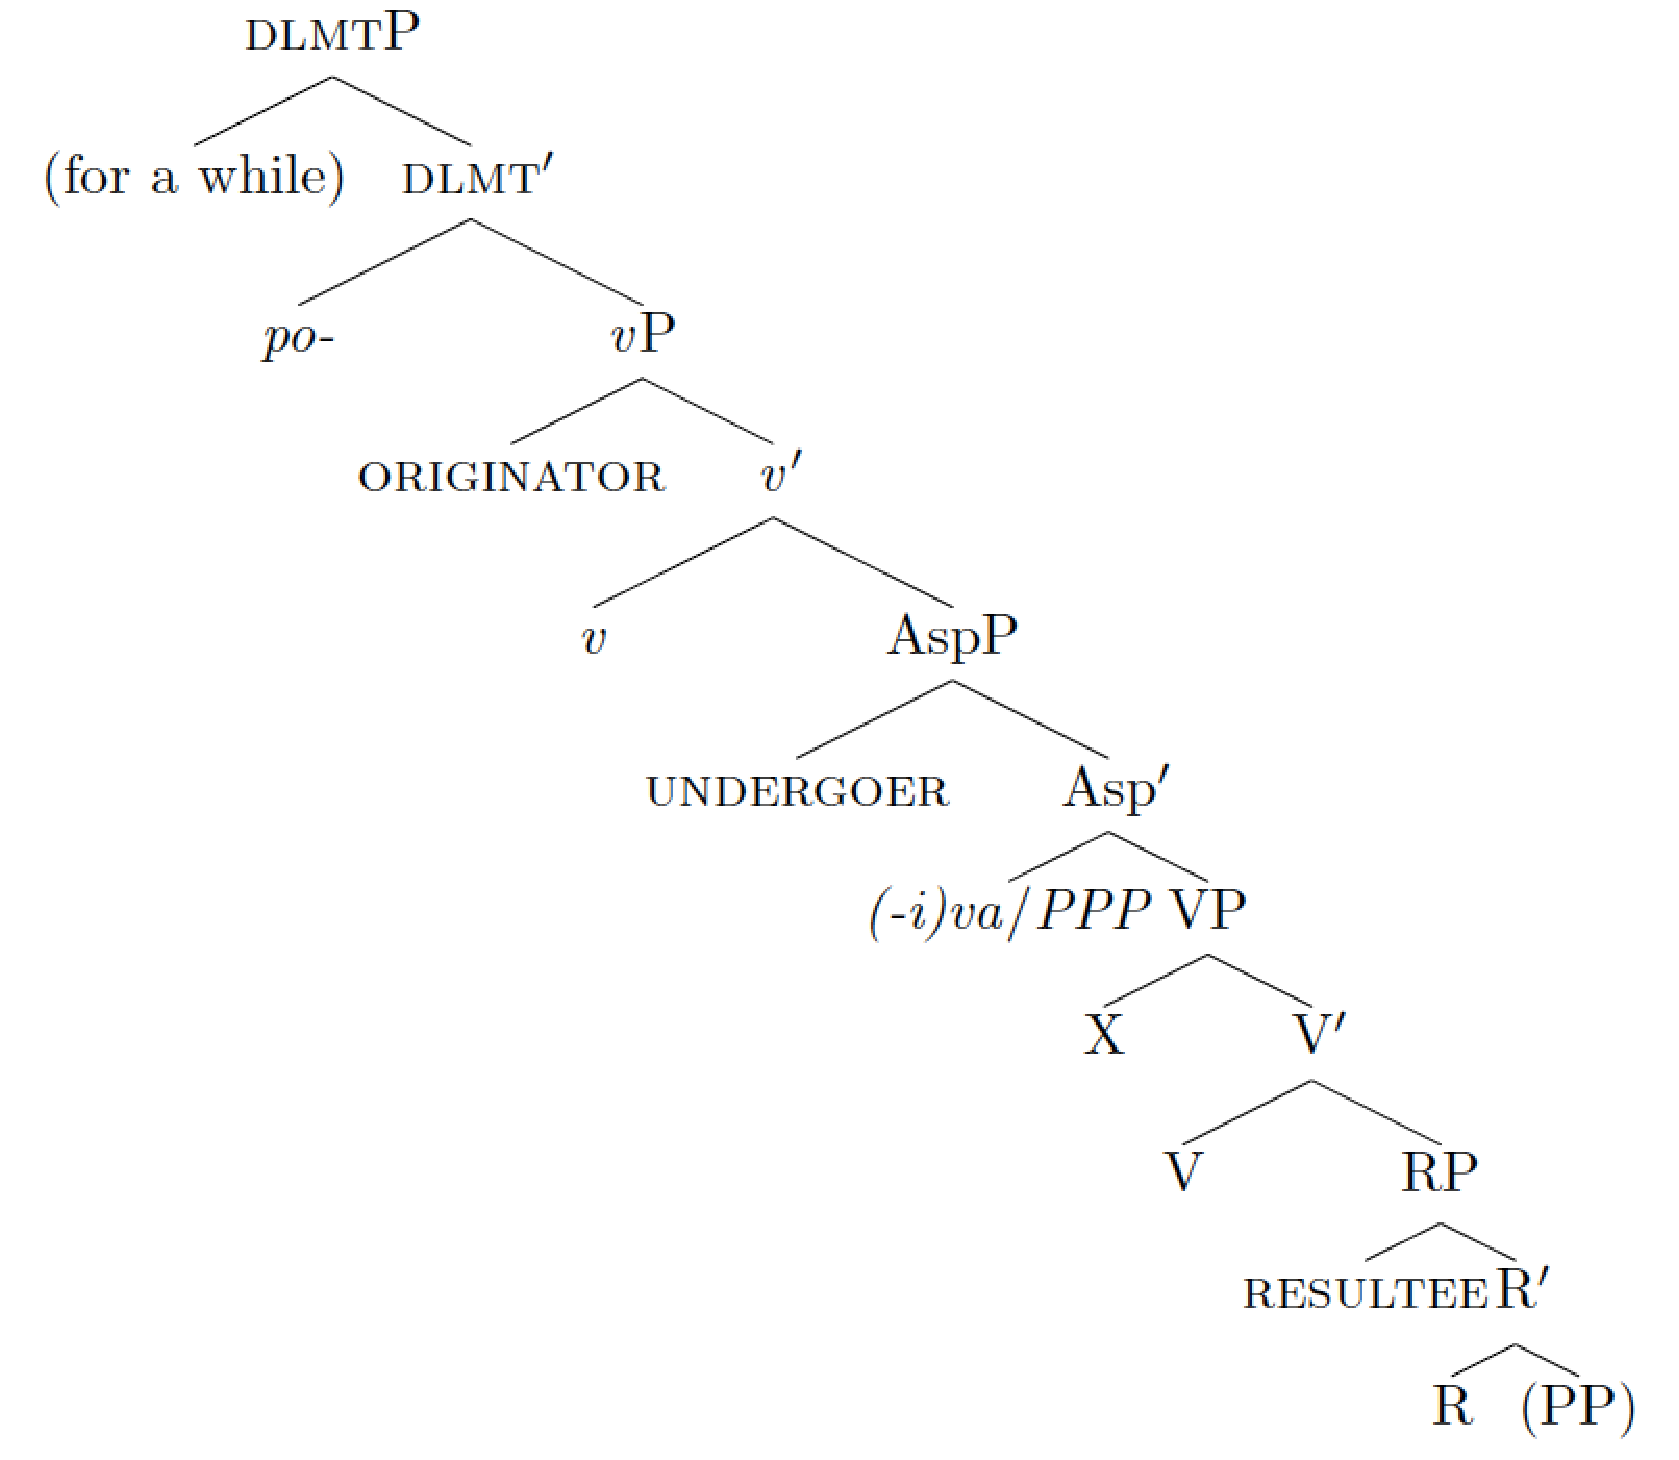
\includegraphics[width=0.8\textwidth]{romanova.pdf}
\caption{\label{fig:romanova} Verbal structure according to \citet[272]{Romanova:04}}
\begin{forest}
[\textsc{dlmt}P
  [(for a while)]
  [\textsc{dlmt}'
    [\Prefix{po-}]
    [\textit{v}P
      [\textsc{originator}]
      [\textit{v}'
        [\textit{v}]
        [AspP
          [\textsc{undergoer}]
          [Asp'
            [\textit{(-i)va}\slash \textit{PPP}]
            [VP
              [X]
              [V'
                [V]
                [RP
                  [\textsc{resultee}]
                  [R'
                    [R]
                    [(PP)]
                  ]
                ]
              ]
            ]
          ]
        ]
      ]
    ]
  ]
]
\end{forest}
\end{figure}

While \citet{Babko-Malaya:99} and \citet{Schoorlemmer:95} (among others) assume that \isi{superlexical} prefixes form a homogeneous class, \citet{Svenonius:04b} argues that there is a tripartite division among \isi{superlexical} prefixes based on their ability to form secondary imperfectives.

According to \citet{Svenonius:04b}, certain \isi{superlexical} prefixes (\Prefix{za-} with inceptive meaning, \Prefix{ot-} with \isi{terminative} meaning, and \Prefix{pere-} with \isi{distributive} meaning\footnote{\Prefix{pere-} has a variety of meanings (e.g. \citealt{Shvedova:82} distinguishes between ten different meanings) including \isi{spatial}, temporal, comparative, iterative, crossing the boundary, \isi{distributive}, and \isi{excessive} \Prefix{pere-}. See Section~\ref{subsection:semantics:pere} for more information.}) may be attached higher than the structural position of the \isi{imperfective suffix}, which is \textit{Asp}, the head of \textit{AspP}. Such prefixes disallow the formation of secondary imperfectives (e.g., \Prefix{za-} in its inceptive use). That is, the \isi{imperfective suffix} cannot be directly attached to an imperfective stem and the result is an invalid structure (see \figref{fig:svenonius}).

There are also mixed cases like \isi{cumulative} \Prefix{na-}, \isi{excessive} \Prefix{pere-}, and \isi{attenuative} \Prefix{po-}. The normal point of attachment of such prefixes, according to \citet[231]{Svenonius:04b}, is outside the scope of the \isi{secondary imperfective}, although under certain exceptional conditions they allow a lower point of attachment.

Svenonius' main generalisations can be stated as follows (see also the summary in \citealt{Svenonius:12}): 

\begin{enumerate}
\item \isi{lexical prefixes} originate inside \textit{v}P;
\item \isi{superlexical} prefixes originate outside \textit{v}P;
\item lexical and \isi{superlexical} prefixes that (according to him) disallow secondary \isi{imperfectivisation} are separated by Asp in the \isi{syntactic structure}; 
\item exceptional \isi{superlexical} prefixes are merged (sometimes) outside \textit{v}P, but below the Asp.
\end{enumerate}

\begin{figure}
% % 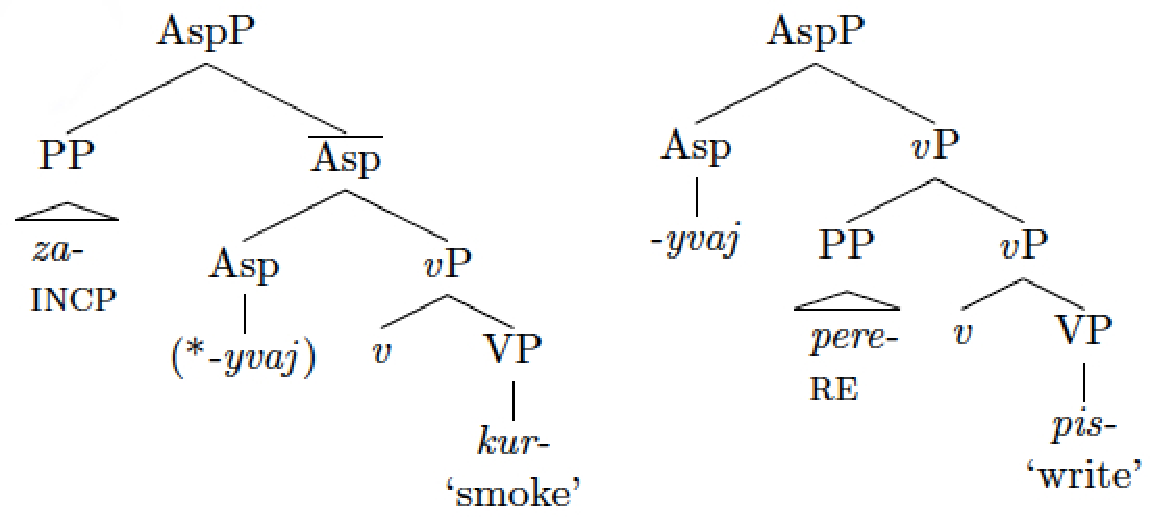
\includegraphics[width=0.8\textwidth]{svenonius.pdf}
\begin{forest}
[AspP
  [PP [\Prefix{za-}\\\textsc{incp},align=center,roof]]
  [$\overline{\mbox{Asp}}$
    [Asp [(*\textit{-yvaj})]]
    [\textit{v}P
      [\textit{v}]
      [VP
        [\textit{kur-}\\`smoke',align=center]
      ]
    ]
  ]
]
\end{forest}
\begin{forest}
[AspP
  [Asp [-\textit{yvaj}]]
  [\textit{v}P
    [PP [\Prefix{pere-}\\\textsc{re},align=center,roof]]
    [\textit{v}P
      [\textit{v}]
      [VP [\textit{pis-}\\`write',align=center]]
    ]
  ]
]
\end{forest}
\caption{\label{fig:svenonius}Verbal structure according to \citet[231]{Svenonius:04b}}
\end{figure}

From another study that follows the same tradition, \citealt{Ramchand:04}, the following ``bottom-up'' order of verbal affixes emerges:

\begin{enumerate}
\item \isi{lexical prefixes};
\item an aspectual head that may contain either the \isi{imperfective suffix} or a \isi{superlexical} prefix;
\item a DP projection for \isi{superlexical} \isi{distributional} prefixes (she cites \textit{pere}- and \textit{po}-). 
\end{enumerate}
While the motivation for this hierarchical order is not entirely clear, it would seem to derive from the following assumptions made by \citet{Ramchand:04}: 
\begin{enumerate}
\item \isi{lexical prefixes} appear low in the \isi{syntactic structure}, due to which a ``presuppositional structure to the aspectual head'' is introduced ``to the effect that it creates a definite rather than an indefinite time moment in Asp'' (p.~349);
\item most \isi{superlexical} prefixes are in Asp and ``impose a specific reference time on the relation between event and temporal anchoring'' (p. 351);
\item a position that \isi{superlexical} prefixes which are \isi{distributional} (\textit{pere}- and \isi{distributive} \textit{po}-) occupy is higher in the hierarchy than the Asp head (p. 352); such prefixes can be attached directly to the root or to the \isi{secondary imperfective} verb.
\end{enumerate}
The fundamental two-way distinction is of key importance for \citet{Romanova:04}, \citet{Svenonius:04b}, and \citet{Ramchand:04}. Putting it simply, the main idea is that \isi{lexical prefixes} occupy lower positions in the \isi{syntactic tree} than the \isi{superlexical} ones. Though it is possible that there is more than one position for \isi{superlexical} prefixes, all such positions should be higher than the one (unique) position for the \isi{lexical prefixes}. 

Due to this syntactic difference, \isi{superlexical} prefixes are claimed to have the following properties:
\begin{enumerate}
\item they provide a systematic semantic contribution and do not change the lexical meaning of the verb;
\item they are incompatible with secondary \isi{imperfectivisation};
\item they do not change the \isi{argument structure} of the verb;
\item they appear to the left of the \isi{lexical prefixes} (if two or more prefixes are stacked). 
\end{enumerate}

Lexical prefixes, on the other hand, are expected to change the lexical meaning of the verb, allow for secondary \isi{imperfectivisation}, change the \isi{argument structure} of the verb, and always appear closer to the stem when \isi{prefix stacking} occurs. At the same time two \isi{lexical prefixes} can never stack, as there is a single position where they are allowed. While specific analyses vary a lot, this general idea remains the same. 

The distinction between the lexical and \isi{superlexical} prefixes has received\linebreak some amount of criticism in the recent literature. For example, \citet{Braginsky:08}, analysing different usages of the prefix \Prefix{za-}, arrives at the conclusion that ``the contrasts
between \isi{inchoative} and non-\isi{inchoative} prefixes \Prefix{za-} cannot be account\-ed for by
simply relating them to different structural positions on the \isi{syntactic tree}'' (p. 224). Let me now analyse in detail properties that are attributed to \isi{superlexical} prefixes and problems that arise when one tries to use the lexical\slash\isi{superlexical} distinction for analysing \isi{complex verbs} in Russian.

%The assumptions listed above lead to the certain predictions about the grammatical aspect of a given complex verb. First, if a verb contains a prefix and no \isi{imperfective suffix}, it is perfective (see ex.~\ref{pred1}). Second, if a verb contains a \isi{lexical prefix} and the \isi{imperfective suffix}, it is imperfective (see ex.~\ref{pred2}). Finally, if a verb contains a \isi{superlexical} prefix and the \isi{imperfective suffix}, it is perfective (see ex.~\ref{pred3}).

\section{Classification ambiguity}\label{section:classification}
The general problem of the lexical/\isi{superlexical} distinction has been pointed out by \citet[32]{Kagan:book}: many prefixes are not easily classified as either lexical or \isi{superlexical} as they do not have the whole cluster of properties of one of the groups, but rather a mixture. This results in a range of classifications offered by different researchers. Table \ref{table:prefixes} summarises various proposals in this respect.


\begin{table}
\caption{Superlexical prefix inventory according to different studies\label{table:prefixes}}
\begin{tabular}{lccccccc}
\lsptoprule
prefix &  \rotatebox{90}{\citet{Babko-Malaya:99}} & \rotatebox{90}{\citet{Svenonius:04a}} & \rotatebox{90}{\citet{Svenonius:04b}\footnote{\citet{Svenonius:04b} provides a classification of Russian prefixes from the point of view of the formation of the \isi{secondary imperfective}, but does not state whether the list is exhaustive.}} & \rotatebox{90}{\citet{Ramchand:04}} & \rotatebox{90}{\citet{Romanova:06}} & \rotatebox{90}{\citet{Tatevosov:09}} & \rotatebox{90}{\citet{Svenonius:12}\footnote{\citet{Svenonius:12} marks the list as taken from \cite{Svenonius:04a}, but the lists vary significantly.}}\\
\midrule
\isi{inchoative} \Prefix{za-} & + & + & + & + & + & + & +\\
\isi{cumulative} \Prefix{na-} & \textminus & + & + & + & + & + & +\\
saturative \Prefix{na-} & \textminus & + & \textminus & \textminus & \textminus & \textminus & +\\
\isi{repetitive} \Prefix{pere-} & \textminus & + & + & \textminus & \textminus & + & +\\
\isi{excessive} \Prefix{pere-} & \textminus & + & + & \textminus & \textminus & \textminus & +\\
\isi{distributive} \Prefix{pere-} & \textminus & \textminus & + & \textminus & + & + & +\\
\isi{distributive} \Prefix{po-} & \textminus & + & \textminus & \textminus & + & + & +\\
\isi{delimitative} \Prefix{po-} & + & + & \textminus & + & + & + & +\\
\isi{attenuative} \Prefix{po-} & \textminus & + & + &  \textminus & \textminus & \textminus & +\\
\isi{attenuative} \Prefix{pri-} & \textminus & \textminus & \textminus & \textminus & + & \textminus & \textminus\\
\isi{attenuative} \Prefix{pod-} & \textminus & \textminus & \textminus & \textminus & + & + & \textminus\\
\isi{terminative} \Prefix{ot-} & \textminus & + & + & \textminus & + & \textminus & +\\
\isi{perdurative} \Prefix{pro-} & + & + &  \textminus & \textminus & \textminus & \textminus & +\\
\isi{completive} \Prefix{iz-} & \textminus & + & + & \textminus & \textminus & \textminus & +\\
\isi{completive} \Prefix{do-} & \textminus & + &  \textminus & + & \textminus & + & +\\
\lspbottomrule
\end{tabular}
\end{table}

The rows of Table~\ref{table:prefixes} show ten prefixes (\Prefix{za-}, \Prefix{na-}, \Prefix{pere-}, \Prefix{po-}, \Prefix{pri-}, \Prefix{pod-}, \Prefix{ot-}, \Prefix{pro-}, \Prefix{iz-}, \Prefix{do-}) together with their interpretations (up to three in case of the prefixes \Prefix{pere-} and \Prefix{po-}). The columns of the table represent seven different proposals: \citealt{Babko-Malaya:99}, \citealt{Svenonius:04a}, \citealt{Svenonius:04b}, \citealt{Ramchand:04}, \citealt{Romanova:06}, \citealt{Tatevosov:09}, and \citealt{Svenonius:12}. A plus in the intersection indicates that the prefix of the row (with the fixed interpretation) is listed as \isi{superlexical} in the work that names the column. As \isi{lexical prefixes} are usually not explicitly listed, a minus in the intersection only indicates that the prefix with specific meaning is not listed as \isi{superlexical}.

As is evident from the table, there is only one prefix that is overtly classified as \isi{superlexical} in all the discussed studies: the \isi{inchoative} prefix \Prefix{za-}. For two more prefixes, \isi{cumulative} \Prefix{na-} and \isi{delimitative} \Prefix{po-}, there is almost complete consensus: all but one study describe them as being \isi{superlexical}. Among the remaining prefixes, there is no single prefix listed as \isi{superlexical} in five out of seven discussed works. After this gap comes a group of prefixes that are accepted as \isi{superlexical} in most accounts represented in the table: \isi{repetitive} \Prefix{pere-}, \isi{distributive} \Prefix{pere-}, \isi{distributive} \Prefix{po-}, \isi{terminative} \Prefix{ot-}, and \isi{completive} \Prefix{do-}. This makes a total of three prefixes in the ``strong'' group and five more in the ``weak'' group. A further seven prefixes are considered \isi{superlexical} only in a couple of studies. Note that there is no pair of works with identical lists of \isi{superlexical} prefixes. 

Such variability in the decisions about which prefix (even under a particular interpretation) falls into one of the two groups (lexical or \isi{superlexical}) clearly shows that this distinction is problematic: the properties that are claimed to be associated with the \isi{superlexical} prefixes do not coincide. I believe that they are not completely independent of each other, but the connection is weaker than is commonly assumed. Let us now discuss different properties attributed to the members of the \isi{superlexical} class of prefixes and see if they are supported by the language data.



\section{Semantics of the derived verb}\label{section:new:compositionality}
The compositionality of meaning is one of the main characteristics of the \isi{superlexical} prefixes, as shown in the summary provided in Section~\ref{section:properties}. It is important to note, however, that this property is not very valuable if we classify prefixes together with certain fixed interpretations. For instance, if one takes into account only \isi{inchoative} usages of \Prefix{za-}, then verbs formed with the \isi{inchoative} prefix \Prefix{za-} will all have the meaning of inception of the activity described by the \isi{derivational base}. All the other \Prefix{za-}prefixed verbs, even if their semantics is perceived as being close to that of inception, will remain outside the focus set of verbs. This means that when the prefix usages are classified, the property of contributing a compositional meaning is reduced to the productivity of a particular meaning of a given prefix. This said, one has to note that many prefixes that are classified as lexical have systematic transparent contributions: e.g., \isi{spatial} prefixes when combined with motion verbs. Consider, in particular, the \isi{spatial} usage of the prefix \Prefix{pere-}, `\isi{to cross}'. Whenever this prefix is attached to a directed \isi{motion verb}, it contributes the meaning `\isi{to cross} something in a manner denoted by the \isi{derivational base}', that can also be reformulated as `to perform the motion denoted by the \isi{derivational base} along the path that crosses the landmark'. However, this prefix (and other similar ones) are not considered \isi{superlexical}.

One may reply at this point, that it is not only the systematic semantic contribution, but the absence of change in the lexical meaning, that distinguishes \isi{superlexical} prefixes from lexical ones. Let us consider the verb \textit{proplyt'}$^{\PF}$ `to swim a certain \isi{distance}' and the verb \textit{proplavat'}$^{\PF}$ `to swim for a certain time'. In the first case we are dealing with the \isi{spatial} interpretation prefix \Prefix{pro-} that is considered to be lexical, while in the second case the same prefix is interpreted temporally and is considered to be \isi{superlexical} by \citet{Babko-Malaya:99}, \citet{Svenonius:04a}, and \citet{Svenonius:12}. Given the semantics of the derived verbs and the possibility of the unified analyses of the prefix \Prefix{pro-} in these cases \citep{Kagan:book, ZinovaOsswald:paper}, it would be very hard to argue that one of these prefixes affects the lexical meaning of the verb, while the other does not. 

\section{Secondary imperfectivisation}\label{section:new:imperfectivization}
Another criterion that is used for establishing the lexical/\isi{superlexical} status of a prefix with a fixed interpretation is the (un)availability of the secondary \isi{imperfectivisation}. Basically, superlexically prefixed verbs should not allow secondary \isi{imperfectivisation} while lexically prefixed verbs should be easily imperfectivised. Unfortunately, things are not as clear and there are exceptions from this rule in both directions. 

To overcome this difficulty, \citet{Svenonius:04b} and \citet{Tatevosov:07, Tatevosov:09} propose to split \isi{superlexical} prefixes into further groups and to distinguish subclasses of \isi{superlexical} prefixes that allow subsequent \isi{imperfectivisation}. Note that in this case the property of used to delimit the classes (nemaly, having potential for further \isi{imperfectivisation}), is not derived from other properties of the prefixes.

Furthermore, as is noted by \citet[35]{Kagan:book}, it is not the case that the availability of the \isi{secondary imperfective} verb can be predicted from the knowledge about the last prefix attached to the verb (and its meaning). Distinct stems, when combined with the same prefix (with a fixed interpretation) behave differently: e.g., the verb \textit{naest’sja} `to eat one's fill' is easily imperfectivised and the combination of the verb \textit{nasmotret'sja} `to spend enough time looking at something' with an \isi{imperfective suffix} is weird (example taken from \citealt[35]{Kagan:book}).

Let us examine the \isi{inchoative} prefix \Prefix{za-} that, according to both \citet[230]{Svenonius:04b} and \citet[116]{Tatevosov:09}, disallows subsequent \isi{imperfectivisation}. Consider the verb \textit{kurit'}$^{\IPF}$ `to smoke'. Which can be prefixed with the \isi{inchoative} prefix {\Prefix{za-}.} The output of \isi{prefixation} is the verb \textit{zakurit'}$^{\PF}$ `to start smoking'. This is a superlexically prefixed verb, according to the common classification, with the most prototypical \isi{superlexical} prefix: the only one which is included in the \isi{superlexical} group in all of the studies I examined. However, this verb can be further imperfectivised. The result of this operation is an imperfective verb \textit{zakurivat'}$^{\IPF}$ `to start/be starting smoking'. As the verb \textit{zakurit'} `to start smoking' denotes a \isi{punctual event}, the natural interpretation of the verb \textit{zakurivat'} `to start/be starting smoking'  is that of a habitual event. Consider example \ref{ex:zakurivat1}. In this sentence the speaker describes his regular activity: after some other event, he always started to smoke and smoked ten cigarettes in a row.\largerpage

\exg.\label{ex:zakurivat1}Ja zakurival i kuril desjat' \v{s}tuk, ne vstavaja s mesta, odnu za drugoj.\\
I za.smoke.imp.\glb{pst}.\glb{sg}.\glb{m} and smoke.\glb{pst.sg.m} ten piece.\glb{pl.acc}, not get.up.imp.\glb{cvb}.\glb{pres} from place, one behind other\\
\trans `I started to smoke and smoked ten cigarettes one after another without getting up.'\hbox{}\hfill\hbox{Vasilij Aksenov, \textit{Zv\"{e}zdnyj bilet}}

At the first sight it seems impossible to interpret the resulting imperfective verb progressively. If this were possible, then a possible solution to the problem could be the one by \citet{Ramchand:04}. \citeauthor{Ramchand:04} suggests that \isi{secondary imperfective} forms with a \isi{habitual reading} may be derived by a different imperfectivising operator from \isi{secondary imperfective} forms with a \isi{progressive reading}. The operator with a \isi{habitual reading} should then be situated higher than the \isi{superlexical} prefix. This proposal does not solve the problem, as it turns out that \isi{progressive interpretation} of the \isi{secondary imperfective} verb containing the \isi{inchoative} \Prefix{za-} is possible. Out of the blue a native speaker of Russian (without linguistic training) would probably deny the existence of such a reading, but all the speakers I have consulted will accept the sentence \ref{ex:zakurivat2}. The trick here is to find some other event (in this case it is a glance) that takes even less time, and hence is ``more punctual''. Then the event of lighting a cigarette can be viewed as a \isi{progressive one}. I will discuss this issue in more detail in the next chapter.

\exg.\label{ex:zakurivat2}Arkadij Sergeevi\v{c} kak raz zakurival, po\`{e}tomu ne zametil, kak na poslednej fraze Olafson po\v{c}emu-to vorovato strel'nul glazami.\\
Arkadij Sergeevich as time za.smoke.imp\glb{.pst.sg.m}, {that is why} not notice.\glb{pst.sg.m}, as on last phrase Olafson {because of something} thievishly shoot.sem.\glb{pst.sg.m} eye.\glb{pl.inst}\\
\trans `Arkadij Sergeevich was just lighting the cigarette, so he didn't notice Olafson's thievish glance during the last phrase.'\\\hbox{}\hfill\hbox{
Andrej Konstantinov, \textit{Vydum\v{s}\v{c}ik}}

Interestingly, while \citet{Tatevosov:09}, along with \citet{Svenonius:04b}, \citet{Ramchand:04}, and others, postulate the impossibility of subsequent \isi{imperfectivisation} of verbs prefixed with \isi{inchoative} \Prefix{za-} (p.~116), the theory described in the paper does not prohibit it, as \Prefix{za-} belongs to the group of prefixes that only attach to \isi{imperfective verbs} (more details will follow in Section~\ref{section:Tat09}). This restriction is met in the example above: the verb \textit{kurit'}$^{\IPF}$ `to smoke' is imperfective. It turns out that for \citet{Tatevosov:09} the only group of prefixes that disallow subsequent \isi{imperfectivisation} is the group of \isi{left periphery} prefixes which comprises only one prefix: \isi{distributive} \Prefix{po-}. This amounts to the fact that one of the main properties of \isi{superlexical} prefixes is attributed to just one prefix which is, moreover, not classified as \isi{superlexical} by some authors.

On the basis of the facts described above I conclude that availability of the \isi{secondary imperfective} form can neither be used for classification purposes nor be reliably predicted from the lexical/\isi{superlexical} status of a given prefix.

\section{Argument structure}\label{section:new:argstructure}
One more property that is said to be associated with \isi{superlexical} prefixes is that they do not change the \isi{argument structure} of the verb (while \isi{lexical prefixes} do). As this criterion is also not unproblematic, \citet[116]{Tatevosov:09}, for example, adopts a milder version of the statement, namely, that \isi{superlexical} prefixes either do not change the \isi{argument structure} of the verb or restrict the possibilities of \isi{argument structure} variation in a predictable way. However, there are exceptions to this property even in the latter formulation. 

The crucial example here is the \isi{cumulative} prefix \Prefix{na-}, which is considered to be \isi{superlexical} in most studies. However, its attachment changes the \isi{argument structure} of the verb: verbs that are optionally transitive when unprefixed become obligatorily transitive after the attachment of the \isi{cumulative} \Prefix{na-}, as illustrated by \ref{ex:pref:na1}--\ref{ex:pref:na2}.

\ex.\label{ex:pref:na1}\ag.\label{ex:pref:na1a}Ma\v{s}a s\v{c}itaet$^{\IPF}$ do desjati.\\
Ma\v{s}a count.\glb{pres.3.sg} until ten\\
\trans `Masha can count up to ten.'
\bg.*Ma\v{s}a nas\v{c}itaet$^{\PF}$ do desjati.\label{ex:pref:na1b}\\
Ma\v{s}a na.count.\glb{pres.3.sg} until ten\\

\ex.\label{ex:pref:na2}\ag.*Ma\v{s}a s\v{c}itaet$^{\IPF}$ desjat' konfet.\label{ex:pref:na2a}\\
Ma\v{s}a count.\glb{pres.3.sg} ten.\glb{acc} candies.\glb{gen}\\
\bg.\label{ex:pref:na2b}Ma\v{s}a nas\v{c}itaet$^{\PF}$ desjat' konfet.\\
Ma\v{s}a na.count.\glb{pres.3.sg} ten.\glb{acc} candies.\glb{gen}\\
\trans `Masha's count of candies will be ten.'

This could be still in accordance with the proposal of \citet{Tatevosov:09}, but it turns out that the prefixed verb also provides an additional restriction on the direct object: it must be a measure phrase. The unprefixed verb \textit{s\v{c}itat'}$^{\IPF}$ `to count\slash be counting' takes as a direct object any plural \isi{accusative noun phrase} (see example \ref{ex:pref:na2a}), whereas the prefixed verb \textit{nas\v{c}itat'}$^{\PF}$ `to count a lot of' does not (see example \ref{ex:pref:na2b}). It requires a measure phrase (example \ref{ex:pref:na3b}), which is not a valid direct object in case of the unprefixed verb \ref{ex:pref:na3a}. 

\ex.\label{ex:pref:na3}\ag.\label{ex:pref:na3a}Ma\v{s}a s\v{c}itaet$^{\IPF}$ konfety.\\
Ma\v{s}a count.\glb{pres.3.sg} candies.\glb{acc}\\
\trans `Masha counts candies.'
\bg.*Ma\v{s}a nas\v{c}itaet$^{\PF}$ konfety.\label{ex:pref:na3b}\\
Ma\v{s}a na.count.\glb{pres.3.sg} candies.\glb{acc}\\

As a result, in all three pairs of examples above involving the verbs \textit{s\v{c}itat'/nas\v{c}itat'} `to count' only one variant (either unprefixed or prefixed) is possible. The unprefixed verb is required in case of an indirect object, as in \ref{ex:pref:na1}, and in case of a direct object that is not a measure phrase, as in \ref{ex:pref:na2}. Only the prefixed verb can be used when the direct object is a measure phrase, as in example \ref{ex:pref:na3}. In fact, there seems to be no construction in which both \textit{s\v{c}itat'} `to count' and \textit{nas\v{c}itat'} `to count a lot of' could be felicitously uttered.

If one considers a pair where the unprefixed verb is obligatorily transitive, as \textit{varit'}$^{\IPF}$ `to cook/be cooking' and \textit{navarit'}$^{\PF}$ `to cook a lot of', it turns out these two verbs require different cases of the object. If the object is an \isi{accusative noun phrase} \ref{ex:pref:navarit:1}, it is only compatible with the unprefixed verb. If it is a \isi{genitive noun phrase}, it is only compatible with the prefixed member of the pair in question, as illustrated by \ref{ex:pref:navarit:2}.

\ex.\label{ex:pref:navarit:1}\ag.\label{ex:varit:1}Ma\v{s}a varit$^{\IPF}$ sup.\\
Ma\v{s}a cook.\glb{pres.3.sg} soup.\glb{acc}\\
\trans `Masha is cooking soup.'
\bg.*Ma\v{s}a navarit$^{\PF}$ sup.\label{ex:navarit1}\\
Ma\v{s}a na.cook.\glb{pres.3.sg} soup.\glb{acc}\\

\ex.\label{ex:pref:navarit:2}\ag.*Ma\v{s}a varit$^{\IPF}$ supa.\label{ex:varit2}\\
Ma\v{s}a cook.\glb{pres.3.sg} soup.\glb{gen}\\
\bg.\label{ex:navarit2}Ma\v{s}a navarit$^{\PF}$ supa.\\
Ma\v{s}a na.cook.\glb{pres.3.sg} soup.\glb{gen}\\
\trans `Masha will cook a lot of soup.'

Interestingly, in the case of the pair \textit{varit'}$^{\IPF}$ `to cook/be cooking' and \textit{navarit'}$^{\PF}$ `to cook a lot of', a measure phrase can be used as a direct object with both verbs, as illustrated by \ref{ex:pref:navarit:3}.

\ex.\label{ex:pref:navarit:3}\ag.\label{ex:varit3}Ma\v{s}a varit$^{\IPF}$ 5 litrov supa ka\v{z}dyj den'.\\
Ma\v{s}a cook.\glb{pres.3.sg} 5 litre.\glb{pl.gen} soup.\glb{gen} every day\\
\trans `Masha cooks five litres of soup every day.'
\bg.\label{ex:navarit3}Ma\v{s}a navarit$^{\PF}$ 5 litrov supa.\\
Ma\v{s}a na.cook.\glb{pres.3.sg} 5 litre.\glb{pl.gen} soup.\glb{gen}\\
\trans `Masha will cook five litres of soup.'

This suffices to show that prefixes that are considered to be \isi{superlexical} can change the \isi{argument structure} of the verb, thereby not only limiting the existing options for the \isi{derivational base} verb, but also adding new ones.

Now we consider the other direction: if the attachment of a \isi{superlexical} prefix can lead to changes in the \isi{argument structure} of the \isi{derivational base} verb, we can try to reformulate the property. An alternative formulation would be to postulate that if a \isi{lexical prefix} is attached to a verb, argument structures of the source and the derived verb will be distinct. This, however, does not work either. As an example, consider the pair of verbs \textit{delat'/sdelat'} `to do'. Both verbs are obligatorily transitive. Illustrations of this fact are provided in \ref{ex:delat} and \ref{ex:sdelat}.

\ex.\label{ex:delat}\ag.Petja delaet$^{\IPF}$ doma\v{s}nee zadanie.\\
Petja do.\glb{pres.3.sg} home.\glb{sg.acc} assignment.\glb{sg.acc}\\
\trans `Petja is doing his homework.'
\bg.*Petja delaet$^{\IPF}$.\\
Petja do.\glb{pres.3.sg}\\

\ex.\label{ex:sdelat}\ag.Petja sdelaet$^{\PF}$ doma\v{s}nee zadanie.\\
Petja s.do.\glb{pres.3.sg} home.\glb{sg.acc} assignment.\glb{sg.acc}\\
\trans `Petja will do his homework.'
\bg.*Petja sdelaet$^{\PF}$.\\
Petja s.do.\glb{pres.3.sg}\\


As one may object that the prefix \Prefix{s-} in \textit{sdelat'} `to do' is what some researchers call an ``\isi{empty prefix}'' (a prefix that changes the aspect, but does not lead to a clear change of the lexical meaning, \textit{\v{c}istovidovaja pristavka} in the Russian tradition), let me provide another example where the prefix is clearly not an ``empty'' one, but, according to those who use the lexical/\isi{superlexical} distinction, a lexical one.  Consider the following three verbs: \textit{nesti}$^{\IPF}$ `to carry', \textit{prinesti}$^{\PF}$ `to carry to some destination',  and \textit{otnesti}$^{\PF}$ `to carry away from some location'. All three verbs have the same \isi{argument structure}: they are obligatorily transitive (see examples \ref{ex:nesti}--\ref{ex:otnesti}).

\ex.\label{ex:nesti}\ag.Petja nes\"{e}t$^{\IPF}$ korobku v podval.\\
Petja carry.\glb{pres.3.sg} box.\glb{sg.acc} in cellar.\glb{sg.prp}\\
\trans `Petja is carrying the box to the cellar.'
\bg.*Petja nes\"{e}t$^{\IPF}$ v podval.\\
Petja carry.\glb{pres.3.sg} in cellar.\glb{sg.prp}\\

\ex.\label{ex:prinesti}\ag.Petja prines\"{e}t$^{\PF}$ korobku v podval.\\
Petja pri.carry.\glb{pres.3.sg} box.\glb{sg.acc} in cellar.\glb{sg.prp}\\
\trans `Petja will carry the box to the cellar.'
\bg.*Petja prines\"{e}t$^{\PF}$ v podval.\\
Petja pri.carry.\glb{pres.3.sg} in cellar.\glb{sg.prp}\\

\ex.\label{ex:otnesti}\ag.Petja otnes\"{e}t$^{\PF}$ korobku v podval.\\
Petja ot.carry.\glb{pres.3.sg} box.\glb{sg.acc} in cellar.\glb{sg.prp}\\
\trans `Petja will carry the box to the cellar.'
\bg.*Petja otnes\"{e}t$^{\PF}$ v podval.\\
Petja ot.carry.\glb{pres.3.sg} in cellar.\glb{sg.prp}\\

This clearly shows that knowing the lexical or \isi{superlexical} status of a prefix is not sufficient to predict whether its attachment will change the \isi{argument structure} of the \isi{derivational base} verb.
\section{Position in the stem}\label{section:new:position}
The least problematic property of \isi{superlexical} prefixes is that they always appear to the left of the \isi{lexical prefixes} if two or more prefixes are stacked. When formulated this way, the property holds. However, a stronger version of this statement is used in the literature, either explicitly \citep{Svenonius:04b} or implicitly \citep{Tatevosov:09}: because there is only one syntactic position a \isi{lexical prefix} can appear in, it is assumed that \isi{lexical prefixes} can only appear directly to the left of the verbal root and cannot be stacked. For example, \citet[206]{Svenonius:04b} writes: ``\isi{lexical prefixes} are unique in each VP, as their structural position is unique -- a single V cannot have more than one \isi{resultative} complement.''


This, however, does not hold. Consider, for example, the verb \textit{razukrasit'} `to decorate' and the verb \textit{razuznat'} `to find out'. Each of these verbs contains two prefixes, \Prefix{raz-} and \Prefix{u-}, both of which are lexical: if one consults Table~\ref{table:prefixes} again, neither of the prefixes is classified as \isi{superlexical} in any of the papers discussed. The derivation chains for the verbs are constructed using the criteria formulated in Chapter~\ref{Chapter2} and provided in \ref{schema:razukrasit'} and \ref{schema:razuznat'}.

\ex.\ag.\label{schema:razukrasit'}krasit'$^{\IPF}$ {$\rightarrow$} ukrasit'$^{\PF}$ {$\rightarrow$} razukrasit'$^{\PF}$\\
{to paint} {} {to embellish} {} {to decorate}\\
\bg.\label{schema:razuznat'}znat'$^{\IPF}$ {$\rightarrow$} uznat'$^{\PF}$ {$\rightarrow$} razuznat'$^{\PF}$\\
{to know} {} {to learn} {} {to find out}\\
\bg.*lo\v{z}it'$^{\IPF}$ {$\rightarrow$} polo\v{z}it'$^{\PF}$ {$\rightarrow$} raspolo\v{z}it'$^{\PF}$\label{schema:raspolozit'}\\
{to put} {} {to put} {} {to position}\\

A similar case is presented in \ref{schema:raspolozit'}
with the difference that in contemporary literary Russian the unprefixed verb \textit{*lo\v{z}it'}$^{\IPF}$ does not exist (it exists in the colloquial language and in dialects). 

From observing these three examples one may, for the sake of saving the hypothesis of a single position for \isi{lexical prefixes}, hypothesise that the prefix \mbox{\Prefix{raz-}/\Prefix{ras-}} is a \isi{superlexical} one. The problem with this hypothesis is that if one believes that the contributions of lexical and \isi{superlexical} prefixes have particular characteristics, then the semantics of this prefix patterns with the semantics of \isi{lexical prefixes}: a thorough study was performed by \citet{JandaNesset:10}, who list eleven subclasses for the meaning that is contributed by the prefix \Prefix{raz-}, and only one of them (Complex Act Perfective in their terminology) is characteristic of the typical contribution of a \isi{superlexical} prefix.

%\iffalse

\section{Subclasses of superlexical prefixes}\label{section:subclasses}
So far we have observed that the binary distinction between lexical and \isi{superlexical} prefixes is not sufficient to predict the existence and properties of verbs containing certain sets of affixes. As at least some of the problems mentioned above were noticed by the researchers working on Russian \isi{prefixation}, several refinements of the original distinction have been proposed in the literature. In further developments of Russian \isi{prefixation} theories we see a shift of focus from the bipartite distinction to the split of the whole class of prefixes into more than two groups: \citet{Tatevosov:07} proposes a \isi{three-way classification} of verbal prefixes and \citet{Tatevosov:09} splits the class of \isi{superlexical} prefixes into three subclasses.

\subsection{Intermediate prefixes}
\cite{Tatevosov:07} introduces a class of \isi{intermediate prefixes} that is supposed to accommodate prefixes which do not fit nicely into either the lexical or the \isi{superlexical} category. This class comprises the \isi{completive} prefix \Prefix{do-} and the \isi{repetitive} prefix \Prefix{pere-}. \citet{Tatevosov:07} proposes that these prefixes are structurally higher than \isi{lexical prefixes}, but lower than \isi{superlexical} prefixes and the \isi{secondary imperfective}. 

This division is motivated by examples like \ref{ex:naperf} and \ref{ex:pereimp}. For the analysis that assumes the two-way classification of prefixes, the verbs \ref{ex:naperf} and \ref{ex:pereimp} have identical \isi{internal} structure: a \isi{superlexical} prefix, a \isi{lexical prefix}, a stem, and the \isi{imperfective suffix}. Nevertheless, these verbs are assigned different aspects: the verb \textit{nazapisyvat'} `to write down a lot' is perfective while the verb \textit{perezapisyvat'} `to be rewriting/to rewrite' is imperfective. For \citet{Tatevosov:07}, there is a structural difference between the two verbs, because \textit{pere}- is classified as an intermediate prefix and is positioned between \isi{lexical prefixes} and the \isi{imperfective suffix}. As a result, the verb in \ref{ex:pereimp} is assigned the imperfective aspect. At the same time, \textit{na}- remains a \isi{superlexical} prefix and thus the verb \textit{nazapisyvat'} `to write down a lot' is assigned the perfective aspect.
\ex.\ag.\label{ex:naperf}nazapisyvat'$^{\PF}$\\
na.za.write.imp.\glb{inf}\\
`to write down a lot'
\bg.\label{ex:pereimp}perezapisyvat'$^{\IPF}$\\
pere.za.write.imp.\glb{inf}\\
`to be rewriting/to rewrite'

However, \cite{Kagan:book} shows that the introduction of \isi{intermediate prefixes} does not solve the problem of predicting the aspect of a given verb on the basis of information about the affixes it is formed with: she provides examples where verbs prefixed with the \isi{attenuative} prefix \Prefix{pod-} allow the subsequent formation of the \isi{secondary imperfective} \citep[35, ex.~\ref{ex:pod} here]{Kagan:book}

\ex.\label{ex:pod}\ag.pod-taj-a-t' - pod-taj-iva-t'\\
pod.melt.\glb{inf} - pod.melt.imp.\glb{inf}\\
melt slightly$^{\PF}$ - melt slightly$^{\IPF}$
\bg.\label{ex:podustavat'}pod-u-st-a-t' - pod-u-sta-va-t'\\
pod.get.tired.\glb{inf} - pod.get.tired.imp.\glb{inf}\\
get tired slightly$^{\PF}$ - get tired slightly$^{\IPF}$
\bg.\label{ex:podzarabatyvat'}pod-za-rabot-a-t' - pod-za-rabat-yva-t'\\
pod.earn.\glb{inf} - pod.earn.imp.\glb{inf}\\
earn some money$^{\PF}$ - earn some money$^{\IPF}$

\citet{Kagan:book} marks imperfective forms in \ref{ex:podustavat'} and \ref{ex:podzarabatyvat'} with \textit{??} and \textit{*} respectively, as out of \isi{context} these forms sound weird to a native Russian speaker. However, if one needs to express the meaning `earn a small amount of money from time to time' the best way to do it is to use the verb \textit{podzarabatyvat'}. As soon as it is put in the \isi{context}, as in \ref{ex:podzarabatyvat'live}, this verb starts to sound natural and may be marked with a question, but is definitely not ungrammatical. I hypothesise that the oddness of the \isi{secondary imperfective} here can be of the same sort as the oddness of multiply prefixed verbs: it is almost impossible to process such verbs without a \isi{context} and thus they are perceived as unnatural when given in isolation, but become fine in an appropriate setting.

\exg.\label{ex:podzarabatyvat'live}Delaete xoro\v{s}ie fotosnimki? U vas est' vozmo\v{z}nost' podzarabatyvat' na \`{e}tom!\\
make good photos near you have possibility pod.za.earn.imp.\glb{inf} on this\\
\trans `Do you take good photos? You have the chance to earn some money from it!' \url{http://smolgorforum.ru/index.php?/forum/65-foto-i-video/}, accessed on 24.08.2021

This suffices to show that the classification provided by \citet{Tatevosov:07} does not allow one to reliably predict the aspect of the complex verb, despite the fact that this task can be viewed as the driving force of the proposed approach. 

\subsection{A three-way distinction}\label{section:Tat09}
%\label{section:selection}
A more elaborate classification is proposed in \citealt{Tatevosov:09}, which is mainly dedicated to the problem of \isi{prefix stacking}. However, in order to account for the relevant stacking constraints, the proposal amounts to a list of postulations about the position of prefixes in the \isi{syntactic tree}. \citet{Tatevosov:09} abandons the previous tripartite distinction among all the prefixes, proposed in \citet{Tatevosov:07}, and instead argues for a classical bipartite division into lexical and \isi{superlexical} prefixes, enriching it with a \isi{three-way classification} of the \isi{superlexical} prefixes in order to account for the relevant facts: \isi{left periphery} prefixes, \isi{selectionally limited prefixes}, and \isi{positionally limited prefixes}.

The group of \isi{left periphery} prefixes comprises only one prefix: \isi{distributive} \textit{po}- (as in \textit{pobrosat'} `to throw all of'). It occupies the \isi{left periphery} of the verbal structure.

Selectionally limited prefixes can be added only to a formally imperfective verb. The group includes the \isi{delimitative} prefix \textit{po}- (\textit{posidet'} `to sit for some time'), the \isi{cumulative} prefix \textit{na}- (\textit{navarit'} `to cook a considerable amount of something'), the \isi{distributive} prefix \textit{pere}- (\textit{perelovit' X} `to catch all of X'), and the \isi{inchoative} prefix \textit{za}- (\textit{zabegat'} `to start running around').

The last group of \isi{positionally limited prefixes} contains the \isi{completive} prefix \textit{do}- (\textit{dodelat'} `to finish doing'), the \isi{repetitive} prefix \textit{pere}- (\textit{perepisat'} `to rewrite'), and the \isi{attenuative} prefix \textit{pod}- (\textit{podustat'} `to become a little bit tired'). These prefixes, according to \citet{Tatevosov:09}, can be added only before\footnote{The attachment of one affix \textit{before} the other is understood in terms of the derivation chain: the first affix is attached at the earlier step of the derivation. This amount to a lower attachment site in terms of the tree structure.} the \isi{secondary imperfective} suffix -\textit{yva-/-iva}- and end up in the same structural position as \isi{intermediate prefixes} in \citet{Tatevosov:07}, the group being extended by one prefix.
	
The net advantage of \citet{Tatevosov:09} over \citet{Tatevosov:07} seems to be that only the former can correctly predict the existence of the derived verbs in \ref{ex:pod} and motivate the difference between \ref{ex:ponaza} and \ref{ex:napoza}. The drawback caused by the need to structurally distinguish cases like \ref{ex:ponaza} and \ref{ex:napoza} is the stipulation that \isi{distributive} prefix \Prefix{po-} forms a singleton group. On \citeauthor{Tatevosov:09}'s (2009) account, \isi{distributive} \textit{po}- must be situated on the \isi{left periphery} of the verb, thus there can be no derivation for \ref{ex:napoza}.
\ex.\ag.\label{ex:ponaza}ponazapisyvat'\\
po.na.za.write.imp.\glb{inf}\\
\trans `to write down all of X one after another'
\bg.\label{ex:napoza}*napozapisyvat'\\
na.po.za.write.imp.\glb{inf}\\

In general, the theory proposed by \citet{Tatevosov:09} seems to account nicely for many cases of multiple \isi{prefixation} of Russian verbs. Let us for the moment set aside the problem of \isi{biaspectual verbs} described in Section~\ref{section:new:biaspectual} as well as the problem of a singleton group, mentioned above, and concentrate on one of the central predictions of the theory: \isi{selectionally limited prefixes} can be attached only to formally \isi{imperfective verbs}.

It turns out that it is possible to find examples where prefixes that are supposed to belong to the selectionally-limited group are attached to formally \isi{perfective verbs}, which contradicts the proposed theory of \isi{prefixation}. We will look in turn at the prefixes \Prefix{po-} (\isi{delimitative}), \Prefix{pere-} (\isi{distributive}), and \Prefix{na-} (\isi{cumulative}). 

\subsubsection{Delimitative \textit{po-}}
First let us consider examples where the \isi{delimitative} prefix \Prefix{po-} can indeed only be added to an imperfective verb. In case of an \isi{aspectual pair} where both verbs are unprefixed (as, for example, \textit{re\v{s}it'}$^{\PF}$\slash\textit{re\v{s}at'}$^{\IPF}$ `to solve') the prefix \Prefix{po-} can only be combined with the imperfective member of the pair (in this case \textit{re\v{s}at'}$^{\IPF}$ `to solve/be solving'), as illustrated by example \ref{ex:po:Tat1} (example (62b) in \citealt[121]{Tatevosov:09}). If the paired verbs both contain a prefix, as \textit{zapisat'}$^{\PF}$\slash\textit{zapisyvat'}$^{\IPF}$ `to write down/record', the \isi{delimitative} prefix \Prefix{po-} is normally attached to the imperfective verb (in this case \textit{zapisyvat'}$^{\IPF}$ `to write down/be writing down'), as illustrated by example \ref{ex:po:Tat2} (example (63b) in \citealt[121]{Tatevosov:09}).

\ex.\label{ex:po:Tat}\ag.\label{ex:po:Tat1}Posidim, *pore\v{s}im (\textsuperscript{\JudgeOK}pore\v{s}aem$^{\PF}$) voprosy, s pacanami poznakomi\v{s}sja, \v{c}toby dorogu slu\v{c}ajno ne perebegat'.\\
po.sit.\glb{pres.1.pl}, *po.solve.\glb{pres.1.pl} (\textsuperscript{\JudgeOK}po.solve.imp.\glb{pres.1.pl}) question.\glb{pl.acc}, with boy.\glb{pl.inst} po.meet.\glb{pres.1.pl}.refl, that road.\glb{sg.acc} {by chance} not pere.run.\glb{inf}\\
\trans `We will sit a bit, solve some issues, you will get to know the boys so that you won't accidentally cross their way.'\\\hbox{}\hfill\hbox{Gennadij Pra\v{s}kevi\v{c}, Aleksandr Bogdan, \textit{\v{C}elovek ``\v{C}''}}\\\hbox{}\hfill\hbox{(62b) in \citet{Tatevosov:09}}
\bg.\label{ex:po:Tat2}Po\`{e}tomu zapustil programmu, zapisyvaju\v{s}\v{c}uju dejstvija na \`{e}krane, otkryl PSP, i nemnogo $^\#$po-zapisal (\textsuperscript{\JudgeOK}po-zapisyval$^{\PF}$), \v{c}to i kak.\\
{because of it} za.let.\glb{pst.sg.m} program.\glb{sg.acc}, za.write.\glb{part.act.pres.sg.f.acc} action.\glb{pl.acc} on screen.\glb{sg.prep}, open.\glb{pst.sg.m} PSP, and {a bit} $^\#$po.write.\glb{pst.sg.m} (\textsuperscript{\JudgeOK}po.write.imp\glb{pst.sg.m}), what and how\\
\trans `For this reason I ran the program that records the actions on the screen and recorded for some time, what was happening and how.'\\\hbox{}\hfill\hbox{=(63b) in \citet{Tatevosov:09}, \url{nova-forum.com}}

Now let me provide some examples where the \isi{delimitative} prefix \Prefix{po-} is attached to a formally perfective verb. In the first example, \ref{ex:popriotkryl}, we are dealing with a selectionally limited prefix \Prefix{po-} that is attached to the perfective verb \textit{priotkryt'}$^{\PF}$ `to open slightly.' The \isi{derivational base} verb already contains the \isi{attenuative} prefix \Prefix{pri-}, so the \isi{delimitative} prefix \Prefix{po-} plays a role of an intensifier of the low degree property. 
\exg. \label{ex:popriotkryl}A na e\v{s}elone on nemno\v{z}ko \v{c}ut' popriotkryl oko\v{s}ko.\\
But at {flight level} he {a little bit} {slightly} po.pri.open.\glb{pst.sg.m} window.\glb{sg.acc}\\
\trans `And at flight level he opened the window just a little bit.'\\\hbox{}\hfill\hbox{\url{http://www.rsdn.ru/forum/life/4244369.1}, accessed on 24.08.2021}

Example \ref{ex:popriotkryl} contains a verb that is the result of attaching the \isi{delimitative} prefix \Prefix{po-} to the perfective verb \textit{priotkryt'}$^{\PF}$ `to open slightly'. We can try to attach the same prefix to the paired imperfective verb \textit{priotkryvat'}$^{\IPF}$ `to open/be opening slightly'. It turns out that the verb that contains all the morphemes of the verb \textit{priotkryvat'}$^{\IPF}$ `to open/be opening slightly' plus the prefix \Prefix{po-} is the verb \textit{popriotkryvat'} `to slightly open some of X'. This verb cannot be substituted for the verb \textit{popriotkryt'}$^{\PF}$ `to open slightly' in \ref{ex:popriotkryl} without changing the meaning of the sentence: \ref{ex:popriotkryval:mod} means that every time the described person flies on the plane, he opens the window. Moreover, the verb \textit{popriotkryvat'} `to slightly open some of X' is imperfective, unlike the verb \textit{pozapisyvat'} `to record for a while' in example \ref{ex:po:Tat2}.

\exg. \label{ex:popriotkryval:mod}A na e\v{s}elone on nemno\v{z}ko \v{c}ut' popriotkryval$^{\IPF}$ oko\v{s}ko.\\
but at {flight level} he {a little bit} {slightly} po.pri.open.imp.\glb{pst.sg.m} window.\glb{sg.acc}\\
\trans `And at flight level he used to open the window just a little bit.'

Another example is provided in \ref{ex:popod-}. Again, the \isi{delimitative} prefix \Prefix{po-} seems to be redundant as it contributes the \isi{delimitative} semantics that is already present in the semantic representation of the \isi{derivational base} (just because this is the condition under which it can be attached).

\exg.\label{ex:popod-}Za sorok let despotizma mozgi popodsoxli.\\
after forty year.\glb{pl.gen} despotism brain.\glb{nom} po.pod.dry.\glb{pst.pl}\\
\trans `During forty years of despotism his brain kind of dried up a bit.'\\\hbox{}\hfill\hbox{\url{http://otvet.mail.ru/question/65535779}, accessed on 24.08.2021}

Like example \ref{ex:popriotkryl}, in example \ref{ex:popod-} it is impossible to substitute the verb \textit{popodsoxli}$^{\PF}$ `dried a bit' with the verb \textit{popodsyxali}$^{\PF}$ `all of them dried a bit' which is derived with an additional step of \isi{imperfectivisation} in between the two prefixations. The modified sentence in \ref{ex:popod-imp} can only be interpreted as the `brain drying' within a group of people, not only with one person.  

\exg.\label{ex:popod-imp}Za sorok let despotizma mozgi popodsyxali.\\
after forty year.\glb{pl.gen} despotism brain.\glb{nom} po.pod.dry.imp.\glb{pst.pl}\\
\trans `During forty years of despotism their brains kind of dried up.'

The conclusion that can be drawn from the examples above is that although in general the \isi{delimitative} prefix \Prefix{po-} attaches to \isi{imperfective verbs}, there are some exceptions to this rule. It also turns out that when we encounter an example of a perfective verb prefixed with the \isi{delimitative} \Prefix{po-}, it is not possible to substitute this verb with the result of the \isi{prefixation} with \Prefix{po-} of the paired imperfective verb without a change in the semantics of the sentence. This means that in cases like \ref{ex:popriotkryl} and \ref{ex:popod-} the perfective verb prefixed with \Prefix{po-} cannot be regarded as a ``variant'' of the verb that obeys the selectional restriction.
 
\subsubsection{Distributive \textit{pere-}}\largerpage[2]
Another prefix that is categorised as selectionally limited by \citet{Tatevosov:09} is the \isi{distributive} prefix \Prefix{pere-}. It turns out that there are examples where this prefix is attached to a formally perfective verb, although on the intuitive level the attachment of a \isi{distributive} \Prefix{pere-} to a perfective verb seems to be more an exception than a rule. Consider the verb \textit{prosit'}$^{\IPF}$ `to ask'. It can be prefixed with a \isi{lexical prefix} \textit{o-}. The result of this \isi{prefixation} is a perfective verb \textit{oprosit'}$^{\PF}$ `to interview'. This verb can be prefixed with the prefix \Prefix{pere-}, producing the verb \textit{pereoprosit'}$^{\PF}$ as the output of the \isi{prefixation}. The question now is, which meaning does \Prefix{pere-} have in this verb? According to \citet{Tatevosov:09}, it could be only iterative \Prefix{pere-}. This meaning is indeed attested, as illustrated by the example in \ref{ex:pereoprosil:iter}, where \textit{pereoprosil} means `interviewed again'.
\exg.\label{ex:pereoprosil:iter}Sledovateli Genprokuratury zanovo pereoprosili u\v{c}itelej i odnoklassnikov Jakova.\\
investigator.\glb{pl.nom} General.Prosecution.\glb{gen} \isi{anew} pere.o.ask.\glb{pst.pl} teacher.\glb{pl.acc} and classmate.\glb{pl.acc} Jakov.\glb{gen}\\
\trans `Investigators from the General Prosecution interviewed the teachers and the classmates of Jakov again.' \url{https://www.topnews.ru/media_id_5978.html}, accessed on 24.08.2021

However, the \isi{distributive} meaning of \Prefix{pere-} is also available: sentence \ref{ex:pereoprosil:distr} is true if the speaker posted on each forum and asked every mechanic only once.

\exg.\label{ex:pereoprosil:distr}Perepostil na vse alfaforumy, pereoprosil vsex znakomyx avtoslesarej.\\ 
pere.post.\glb{pst.sg.m} on all {alfa.forums}, pere.ask.\glb{pst.sg.m} all.\glb{acc} known mechanic.\glb{pl.gen}\\
\trans `I posted it on all the major forums and asked all mechanics I know.' \url{https://fiat-club.org.ua/forum/viewtopic.php?t=27668}, accessed on 24.08.2021

Let us now consider the case of attaching the prefix \Prefix{pere-} to an imperfective verb. The verb \textit{oprosit'}$^{\PF}$ `to interview' can be imperfectivised, providing a paired verb \textit{opra\v{s}ivat'}$^{\IPF}$ `to interview/be interviewing'. If this verb is prefixed with \Prefix{pere-}, the result of the \isi{prefixation} is the verb \textit{pereopra\v{s}ivat'}$^{\PF}$ `to interview all of'. An example of the usage of this verb, found on the internet, is provided in \ref{ex:pereoprashival}. Like in \ref{ex:pereoprosil:distr}, it is clear from the \isi{context} that each of the scientists was asked separately and only once. Normally in a similar \isi{context} one would use the verb \textit{perespra\v{s}ivat'}$^{\PF}$ `to ask all of', as \textit{spra\v{s}ivat'}$^{\PF}$ `to ask' refers to an individual question and the prefix \Prefix{pere-} then provides iteration over the referents. On the other hand, the verb \textit{opra\v{s}ivat'}$^{\PF}$ `to interview' already encodes iteration of the questions, so after the attachment of the distibutive \Prefix{pere-} the resulting verb denotes an event that contains a double iteration: every respondent is asked every question. In case of \ref{ex:pereoprashival}, the speaker (or his hero in the computer game the forum is about) asked any other characters of the ``scientist'' type all the possible questions (limited by the game design).\largerpage

\exg.\label{ex:pereoprashival}Pereopra\v{s}ival vsex u\v{c}\"{e}nyx, nikto ne da\"{e}t kvest na oazis...\\
pere.o.ask.imp.\glb{pst.sg.m} all.\glb{acc} scientist.\glb{pl.gen}, nobody not give.\glb{pres.3.sg} quest on oasis.\glb{sg.acc}\\
\trans `I've talked (asked all the questions) to all the scientists, none of them gave me the oasis quest.' \url{https://antistarforce.com/forum/69-3832-26}, accessed on 24.08.2021

\subsubsection{Cumulative \textit{na-}}
An interesting discussion can be found in \citet{Tatevosov:13a}. It concerns the possibility of attaching the \isi{cumulative} prefix \Prefix{na-} to a perfective verb. Citing \citet{Zaliznjak:03}, \citet{Tatevosov:13a} concludes that there is a closed list of verbs consisting of a perfective stem prefixed with the \isi{cumulative} \Prefix{na-} that are accepted by all Russian native speakers. \citet{Tatevosov:13a} mentions, for instance, the verbs \textit{nakupit'}$^{\PF}$ `to buy a lot of something' and \textit{napustit'}$^{\PF}$ `to fill something with a lot of something'. 

\citeauthor{Tatevosov:13a} also writes, however, about another, much larger group of verbs that are formed according to this pattern. This group, according to him, includes such verbs as \textit{napridumat'}$^{\PF}$ `to come up with a lot of something', \textit{narasskazat'}$^{\PF}$ `to tell a lot of something', and \textit{naso\v{c}init'}$^{\PF}$ `to write/compose a lot of something'. Consider example \ref{ex:nazapostil}, taken from the internet. Here we see two verbs formed by \isi{prefixation} of a perfective verb with the \isi{cumulative} prefix \Prefix{na-}: \textit{naotkryt'} `to open a lot of X' and \textit{nazapostit'} `to write and publish a lot of posts.'
 
\exg.\label{ex:nazapostil}I naotkryl i nazapostil mnogo tem.\\
and na.open.\glb{pst.sg.m} and {na.write.\glb{pst.sg.m}} {many} {topics}\\
\trans `And started a lot of posts and wrote about a lot of topics.' \url{http://forum.hayastan.com/lofiversion/index.php/t5328-100.html}, last accessed in 2016

\citet{Tatevosov:13a} claims that there is quite a large group of people who speak a dialect of Russian where the \isi{cumulative} prefix \Prefix{na-} lacks any \isi{syntactic restrictions} and can be freely attached to \isi{perfective verbs}. Two problems arise with this claim.

First, the distinction between the ``major'', more restrictive dialect and the dialects that allow freer attachment of the \isi{cumulative} \Prefix{na-} seems to be not so clearcut. For example, for me as a native speaker of Russian there is a difference in the acceptability of the two verbs in \ref{ex:nazapostil}: the verb \textit{naotkryt'} `to open a lot of X' seems to be considerably less acceptable than the verb \textit{nazapostit'} `to post a lot'. This may be due to the fact that the verb \textit{naotkryt'} `to open a lot of X' can be replaced by another verb in which the \isi{cumulative} \Prefix{na-} is attached to the imperfective stem: \textit{naotkryvat'}$^{\PF}$ `to open a lot of X' derived from \textit{otkryvat'}$^{\IPF}$ `to open/be opening'. The verb \textit{nazapostit'} `to post a lot', however, lacks a similar paired verb: if I try to form a \isi{secondary imperfective} from the verb \textit{zapostit'} `to post', none of the resulting forms sounds acceptable, possibly for phonological reasons: $^?$\textit{zapostivat'}, $^?$\textit{zapos\v{c}ivat'}, $^?$\textit{zapo\v{s}\v{c}ivat'}, $^?$\textit{zapo\v{s}\v{c}\v{s}\v{c}ivat'}. Interestingly, all of these forms are attested on the internet, as evidenced by the examples in \ref{ex:zapostivat} (with the third variant, \textit{zapo\v{s}\v{c}ivat'}, being the most frequent).

{\sloppy
\ex.\label{ex:zapostivat}\ag.Ix teksty ja zapostival na na\v{s} fakul'tetskij forum.\\
they.\glb{gen} text.\glb{pl.acc} I za.post.imp.\glb{pst.sg.m} on our department.\glb{sg.acc.m} forum.\glb{sg.acc}\\
\trans `Their texts I've posted on the forum of our department.'\\\hbox{}\hfill\hbox{\url{hgr.livejournal.com}, last accessed in 2016}
\bg.Tak ponevole bude\v{s} prosit' razre\v{s}enija, esli u\v{z}e raz zapos\v{c}ival, tak pot\"{e}rli.\\
so unwillingly will.\glb{2.sg} ask.\glb{inf} permission.\glb{sg.acc}, if already once za.post.imp.\glb{pst.sg.m}, so po.rub.\glb{pst.pl}\\
\trans `If you already posted something once and it was erased, you inevitably start to ask for permission.' \url{https://www.forumavia.ru/t/172787/1/}, accessed on 24.08.2021
\bg.Davnen'ko ja ni\v{c}ego ne zapo\v{s}\v{c}ival, no dejstvitel'no pisat' ne o \v{c}em.\\
{quite a while} I nothing not za.post.imp.\glb{pst.sg.m}, but really write.\glb{inf} not about that.\glb{prp}\\
\trans `I haven't posted anything for quite a while, but I really have nothing to write about.'\hbox{}\hfill\hbox{\url{www.drive2.ru}, last accessed in 2016}
\bg.Reporta\v{z} 1 kanala RF o poxoronax desantnika ja u\v{z}e zapo\v{s}\v{c}\v{s}\v{c}ival.\\
reportage.\glb{sg.acc} 1 channel {Russian Federation} about funeral.\glb{prp} paratrooper.\glb{sg.gen} I already za.post.imp.\glb{pst.sg.m}\\
\trans `I've already posted the documentary of the first federal channel about the funeral of a paratrooper.' \url{waronline.org}, last accessed in 2016

}\noindent The fact that all the possible variants of forming a \isi{secondary imperfective} from the verb \textit{zapostit'} `to post' are attested on the internet indicates that neither of these variants is perfect and acceptable by all speakers.

Now let us explore another problem that arises if we postulate the absence of any restrictions on the attachment of the prefix \Prefix{na-} for some dialects of Russian, as \citet{Tatevosov:13a} does. The speakers of such a dialect should be able, for example, to derive the verb \textit{naotkryt'}$^{\PF}$ `to open a lot of X' and then imperfectivise it by the attachment of the suffix \is{suffix!imperfective suffix}\textit{-yva-}, deriving an imperfective verb $^*$\textit{naotkryvat'}$^{\IPF}$ `to open/be opening a lot of X'. However, the internet data do not supply any single attestation of the imperfective aspect for the verb \textit{naotkryvat'} `to open a lot of X'. This is unexpected if one assumes the theory proposed in \citet{Tatevosov:13a} without further restrictions.\largerpage

In sum, three out of four prefixes in the selectionally limited group proposed by \citet{Tatevosov:09} do not strictly obey the selectional restriction. 

\section{Conclusion}\label{section:new:conclusion}
In this chapter we have seen that none of the properties of the lexical and \isi{superlexical} prefixes that are predicted on the basis of their syntactic position is universal. This leads to the conclusion that on the basis of the properties of the prefixes that we know so far it is impossible to postulate a clear-cut distinction between the different groups. 

This is not to negate the existence of various types of prefixes associated with particular properties. For instance, some prefixes (in all their usages) always contribute a regular meaning that can be derived \isi{compositionally}, and the contribution of others to the semantics of the complex verb is obscure. The key point that I would like to emphasise is that there is no natural cut-off between one group of prefixes and the other. It looks much more like a continuous scale on which the prototypical \isi{lexical prefixes} are at one end, the prototypical \isi{superlexical} prefixes are at the other end, and most prefixes are somewhere in between. 

Such an approach to the classification of prefixes allows to build on the insights about the varying behaviour of distinct types of prefixes and at the same time not to be committed to drawing a line between these types, as this seems to create problems instead of solving them. On the other hand, assuming such a continuum means that it is not possible to assign each prefix a fixed position in the \isi{syntactic tree}. In what follows I will show that it is possible to account for a range of facts that were shown as problematic in this chapter by replacing some of the \isi{syntactic restrictions} with \isi{semantic restrictions}.
 % Limitations of existing approaches
% Chapter 5
\chapter{Semantics of individual prefixes} % Write in your own chapter title
\label{Chapter5}
%\lhead{Chapter 4. \emph{Semantics of individual prefixes}} % Write in your own chapter title to set the page header
\section{Semantic approach to verbal prefixation}
The main things that we have discussed so far are an efficient way of collecting and verifying the data and the fact that these data cannot be fully accounted for by means of existing syntactic approaches to Russian prefixation. Let us now explore what has been done in the domain of prefix semantics.

Semantics-oriented studies of Russian prefixes can be divided in three groups: (i) studies following the Russian tradition that investigate nuances of different prefix usages, (ii) studies following the ``Western'' tradition that aim to find uniform semantics (or one function) for all the prefixes (not only in Russian, but in Slavic languages in general), and (iii) studies that try to bridge the gap between the first two approaches. Let me provide a bit more detail about each of these directions of research.

The main question that is addressed in the Russian tradition is nicely formulated by \citet[18]{Boguslawski:63}, who writes that ``the problem of defining all the meanings of `the same prefixes' is first of all a practical problem and is of a great importance for the lexicographic studies". The main purpose of the grammar \citep{Grammar:52, Shvedova:82} and dictionaries \citep{Dict:50, Dict:57}, as well as of many other studies of Russian prefixes (\citealt{Avilova:64, Golovin:59, Lopatin:97, Tixonov:98}, among others) is to examine the data in great detail and provide a full picture of the different usages that a particular prefix may have. As a next step, the type of relation (polysemy of homonymy) between these usages is analysed \citep{Krongauz:97, Plungyan:01}. This work is necessary, but its focus is on descriptive adequacy and not on finding differences or similarities between different prefixes or explaining why a particular combination of stacked prefixes is available or not.

As for the ``Western'' approach, the main idea they exploit is that Slavic verbal prefixes are markers of perfective aspect (\citealt[see, e.g.,][]{Binnick:91, Krifka:92, Zucchi:99}, among others). Perfective aspect itself then gets analysed in terms of quantisation (first proposed in \citealt{Krifka:86, Krifka:92}, and later repeated by \citealt{Pinon:95}), from which it follows that the semantic function of verbal prefixes is to contribute quantisation, defined by \citet{Krifka:86} as shown in \defref{def:quant}. 

\theoremstyle{definition}
\begin{definition}{Quantisation}\label{def:quant}
\textit{QUA(P)} $\leftrightarrow \forall x,y[P(x) \wedge P(y) \rightarrow \neg y<x]$\\
A predicate \textit{P} is quantised iff, whenever it applies to \textit{x} and \textit{y}, \textit{y} cannot be a proper part of \textit{x}.
\end{definition}

However, \citet{Filip:92} noticed that matters are more complicated, as there are perfective verbs that fail to be quantised according to the \defref{def:quant}. \citet{Filip:92} raised a number of questions in this respect, and proposed that ``the semantic property of the Incremental Theme NPs that is determined by aspect should not be characterized in terms of the `cumulative/quantised' distinction, but rather in terms of the `bounded/unbounded' distinction, which characterizes aspect \citep[][147]{Filip:92}.

In a next step, \citet{Filip:92} shifted the focus to the contribution of the Slavic linguistic tradition \citep{Wierzbicka:67, Rassudova:75, Merrill:85} and concluded that verbal prefixes must be associated with local quantificational effects\footnote{A-quantification in terms of \citealt{BachPartee:87, BachPartee:95}, which is typically expressed at the sentence level or at the level of VP with sentence adverbs, ``floated'' quantifiers (e.g., \textit{each}), verbal affixes, auxiliaries, and various argument-structure adjusters.} (among other meaning components). \citet{Filip:99} later proposes to analyse Slavic verbal prefixes as scalar expressions. This became a departure point for the subsequent analyses \citep{Filip:00, Filip:03, Filip:05, FilipRothstein:05, Kagan:11, Kagan:12, Kagan:13, Kagan:book}. For example, \citet[183]{Filip:99} writes that the prefix \Prefix{na-} ``adds to a verb the meaning of a sufficient or large quantity, or a high degree measured with respect to a certain contextually determined scale and with respect to some standard or subjective expectation value.'' Later, \citet{Filip:08} also formulated the general idea that prefixes (at least under certain usages) ``contribute to the specification of the ordering criterion on events'' and proposed to include them in the class of scale inducing expressions. This idea allowed \citeauthor{Kagan:12} (\citeyear{Kagan:12}, \citeyear{Kagan:book}) to further develop the semantic approach to prefixation under which ``the major semantic function of a prefix is to impose a certain relation between two degrees on a scale''. Various prefixes then differ with respect to the type of the scale they can apply to and the exact relation between the degrees  they establish. 

Following \citet{Filip:08}, the idea of scalar interpretation of verbal prefixes serves as a bridge between the two traditions: on the one hand, it reveals the common core of the prefixes, and on the other hand, it provides the space for explaining the distinctions between individual prefix usages. 

I propose to use a scalar approach to prefix semantics in order to account for another complex issue: prefix combinatorics. \citet{Tatevosov:09} correctly notices that descriptive approaches and structuralist theories of the semantics of Russian prefixes, such as \citet{Avilova:64}, \citet{Golovin:59}, \citet{Lopatin:97}, and \citet{Tixonov:98}, did not bring us closer to the understanding of how complex verb formation operates. On this basis, \citet{Tatevosov:09} concluded that a semantic approach is not helpful for predicting the existence and properties of complex verbs. This conclusion is, however, not a valid one: an inspiring counterexample is the work by \citet{Filip:03}, who uses the `one delimitation per event' constraint to motivate the exclusion of some prefix-verb combinations on semantic grounds. This constraint is formulated by \citet[79]{Tenny:94} as ``[t]he event described by a verb may only have one measuring-out and be delimited only once''. It is grounded in the independent restrictions that come from the grammar of measurement in natural languages and it operates across both nominal and verbal domains. 

Taking this as a point of departure, I propose to analyse certain restrictions on the formation of complex verbs as semantic restrictions. As I have shown in Chapter~\ref{Chapter2} and Chapter~\ref{Chapter4}, a significant amount of data cannot be treated adequately in the syntactic approaches: biaspectual verbs, stacking of prefixes, formation of secondary imperfective verbs. I propose to look at these processes from a different angle, taking into account the semantics of verbal prefixes. I will show that the scalar semantic approach can be successfully used to motivate stacking of prefixes (as well as the existence of biaspectual verbs and certain restrictions on the formation of secondary imperfective verbs). A formalism that allows us to restrict derivations on the basis of semantic constraints is then required. 

%My intuition here is similar to that of \citet{Kagan:book}: prefixes are related to scales and introduce some delimitation of events. Due to these delimitations events may become telic and perfective. 

%This intuition is also related to other ways of thinking about prefixation presented in the literature, including syntactic accounts. For example \citet{Tatevosov:09} constraints prefixes in the selectionally limited group in that they cannot be attached to a formally perfective verb. In the account I propose, the impossibility of such an attachment is explained via the incompatibility of the semantic restrictions associated with the verb and the prefix. This explains those cases that are exceptional from the syntactic point of view, as it turns out that semantic restrictions are compatible. This is, for example, the case of combining two prefixes with the delimitative function: the delimitative prefix \Prefix{po-} cannot be attached to a perfective verb, unless this verb is already prefixed with another delimitative prefix. We will discuss such examples in detail later in this chapter.
 
%The crucial difference between the previous semantic accounts of Russian verbal prefixation and this work is the different formulation of the research question and the formalization of the semantics of prefixes, which will be provided in Chapter~\ref{Chapter7}. An important property of the formal part of the account is its capability to grasp by means of the semantic representation not only the semantics the prefix contributes to the derived verb, but also the semantic restrictions on its attachment. In this chapter I will prepare the ground for this formalization, providing informal descriptions of the semantics and attachment restrictions of individual prefixes after carefully investigating their properties. 

The goal of this chapter is to motivate intuitions about the behaviour of individual prefixes and provide informal semantic analyses of the prefixes under discussion in such a way that their combinatorial properties derive naturally from their semantic properties. 
This discussion provides the basis for the formalisation of prefix semantics that will follow in Chapter~\ref{Chapter7}. The prefixes that we are going to look at are the following: \Prefix{za-} (inchoative usage), \Prefix{na-} (accumulative usage), \Prefix{po-} (delimitative and distributive usages), \Prefix{pere-} (iterative, distributive, and excessive usages), and \Prefix{do-} (completive usage). I will occasionally mention some of the extra usages of the discussed prefixes, but analysing them, as well as other prefixes, is beyond the scope of this book.

For each prefix, the structure of the respective subsection is the same, covering three important issues and followed by a summary:
\begin{enumerate}
\item semantic contribution;
\item restrictions on the attachment: (in)compatibility of lexical semantics of verbal stems with prefix semantics;
\item subsequent imperfectivisation of a verb with the discussed prefix;
\item summary.
\end{enumerate}

%In the sections \ref{subsection:semantics:za}-\ref{subsection:semantics:do} I discuss contributions of individual prefixes on the pre-formal level. This discussion provides the basis for the formalization of prefix semantics. The goal of the formalization I propose is not only to adequately capture the semantics of the discussed prefixes, to be able to predict whether verbs containing certain combinations of a verbal root and prefixes exist and which aspect and semantics such verbs have. 

Before we proceed, I would like to note that shifting the focus from the syntactic restrictions to the semantic ones in the domain of prefix stacking does not mean that no syntactic theory of verbal structure is needed. There still remain constraints that are better formulated in (morpho-)syntactic terms. An example of such a constraint is the unavailability of multiple imperfective suffixes in Russian. 

Another module that is involved in regulating complex verb formation in Russian is pragmatics. I propose some preliminary pragmatic explanations for the non-existence of certain verbs in this chapter and provide some more details in Chapter~\ref{Chapter6}.

As scales are crucial in the analysis of the prefixes, let me provide a brief overview of the concept before discussing the properties of individual prefixes.

\section{Scales}

%Studies that look at the relation between telicity and either measure (Tenny 1994), or scale (Filip 93/99, 2004, Hay, Kennedy, Levin 99, Beavers 06, 07, Wehsler 05), or incremental theme (Dowty 91, Krifka 89, 92,98), or quantity criterion (Filip 2005), or ordering criterion (Filip-Rothstein 06)

%Rappaport Hovav: three kinds of scales recognized in the literature: property scales, path scales, volume/extent scales
The original area of application of scales in linguistics is the domain of gradable adjectives. As suggested by \citet{Kennedy:99}, gradable adjectives (e.g., \textit{wide, tall, expensive}) denote properties that for different individuals hold to different degrees. This means that they are analysed as denoting a certain relation between an individual-type and a degree argument. One formalisation of this idea is that an adjective lexicalises a \textit{scale} and maps its argument to a certain degree on that scale \citep{Kennedy:01, KennedyLevin:02}. An alternative formalisation \citep[e.g.,][]{Heim:00} represents such adjectives as taking a degree as an argument and providing as its output the set of the individuals for which the lexicalised property holds up to this degree.

 A \textit{scale} is defined as a set of points (degrees, values), %\footnote{The term \textit{degree} is used to refer to either points or intervals on the scale (see, e.g., \citealt{KennedyMcNally:05}), so we will refer to the either points or values on the scale to avoid confusion.}
 totally ordered along some \textit{dimension} (e.g., length, quantity, volume, duration). If the scale has maximal and minimal elements, it is a \textit{totally closed} scale (often called just \textit{closed} scale). If the scale has neither a maximal nor a minimal element, it is a \textit{totally open} (or just \textit{open}) scale. Scales that have a minimal and lack the maximal element are \textit{lower closed} and scales that lack the minimal and have the maximal element are \textit{upper closed}. These properties play an important role in accounting for the adjectival semantics \citep[see, e.g.,][]{KennedyMcNally:05, RotsteinWinter:04, KaganAlexeyenko:10}.
 
Other central notions in this domain are that of \textit{comparison class} and \textit{standard of comparison}. The relevant comparison class \citep[see, e.g.][]{Klein:80, KennedyMcNally:05, Kennedy:07} is constituted of objects similar to the individual argument in the relevant respects. The comparison class then provides the standard of comparison and the sentence like \ref{ex:expensive} is interpreted as asserting that the price of the house is higher then the standard price of a house from the comparison class (houses with similar parameters in the same area).
 
 \ex.\label{ex:expensive}This house is expensive.

Comparative adjectives, such as in \ref{ex:expensive:more}, differ in that they overtly specify the comparison class and, thus, the standard of comparison. 

 \ex.\label{ex:expensive:more}This house is more expensive than the one we saw yesterday.
 
Differential degrees (\citealt{Kennedy:01}, also called difference values in \citealt{KennedyLevin:02}) and the operation of degree addition \citep{KennedyLevin:02} allow to represent the semantics of such sentences as \ref{ex:expensive:more:1000} by explicitly stating how the relevant degrees of the individuals are related.
 
 \ex.\label{ex:expensive:more:1000}This house is five thousand dollars more expensive than the one we saw yesterday.

The scalar approach to the semantics of event predicates has proven to have a considerable explanatory power and has been advocated in numerous works on event semantics \citep[see, e.g.,][]{Ramchand:97, Hay:99, KennedyLevin:02, CaudalNicolas:05, FilipRothstein:05, Kearns:07, KennedyLevin:08, Filip:08, Pinon:08, Rappaport:08, Rappaport:11, McNally:11}. Let me provide a very brief overview of the works that adopt a scalar approach in order to account for the aspectual properties of event predicates (for a more detailed observation and extra references see \citealt{Arsenijevic:13}).

The first class of verbs that has been explored from the scalar semantics perspective is the class of degree achievements, such as \textit{cool}, \textit{grow,} or \textit{widen}. The crucial difference between adjectives and degree achievement verbs is that while the former map individuals to degrees, the latter denote a change in degree: the degree to which the argument possesses the property at the end of the event is higher than at the beginning. Therefore, a temporal argument has to be introduced \citep{Hay:99, KennedyLevin:02}.

%\ex.\label{ex:Kennedy2}\a.Kim walked from the bank to the store in/??for an hour.
%\b. Kim walked for/??in an hour.\\
%= (4.4) in \citealt{Kennedy:12}, p. 104

In a next step, scalar approaches to degree achievements were integrated with earlier approaches to the aspectual composition. The theory of aspectual composition has been developed based on the observations about the behaviour of \textit{incremental theme} verbs. Such verbs are characterised by referring to eventualities that involve an incremental change that is related to the internal argument \citep[see][]{Garey:57, Wierzbicka:67, Verkuyl:72, Krifka:86, Krifka:92, Filip:92, Filip:99}. An example of a verb of an incremental creation is provided in \ref{ex:Kennedy1}. An important observation is that when the incremental theme has some specified quantity, the predicate is telic; when there is no such specification, the predicate is atelic.

%verbs of directed motion (as \textit{ascend}) and  were included in the class of verbs that receive scalar interpretation. Verbs of motion, according to this view, are associated with an increase of a degree on the \textit{path} scale. Incremental theme verbs 

\ex.\label{ex:Kennedy1}\a. Lee wrote a poem in/??for an hour. \hfill telic
\b. Lee wrote poetry for/??in an hour. \hfill atelic\\
\hbox{}\hfill\hbox{= ex.~(4.1) in \citealt[103]{Kennedy:12}}


%The analysis of incremental theme verbs has been later generalized to capture other types of verbs that demonstrate similar behavior: motion verbs, as in \ref{ex:Kennedy2}, and 
%
%\ex.\label{ex:Kennedy3}\a. The canyon widened 30 kilometers in/??for one million years.
%\b. The canyon widened for/??in one million years.\\
%= (4.5) in \citealt{Kennedy:12}, p. 104

Later, \citet{Filip:05} has shown that the basic meaning of an incremental theme verb in English does not introduce a scale. This approach has been adopted by \citet{Rappaport:08}, \citet{LevinRappaport:10}, \citet{Kennedy:12}, and \citet{Bochnak:13} who concluded that measure of change functions must be associated with the incremental theme arguments. These arguments then supply some value that is used to select an appropriate portion of the scale that has to be covered in course of the event. 

Now let us describe additional kinds of scale types that will be relevant for the following discussion. First of all, I want to distinguish two types of situations involving a change along a scale: for the first type, the absolute value on the scale matters, and for the second type, the absolute values are not important and we are only interested in the difference between the values at the beginning and at the end of the event. For example, if John heated the water up to 40 degrees Celsius, it is the absolute value that matters, and if John gained 2 kilos it is the difference that is relevant. We will say that the first event proceeds along the \textit{temperature} scale (I will call the class of such scales \textit{proper scales}) and the linguistic context supplies the \textit{maximum value} on that scale. In the second case, we will say that the event proceeds along the \textit{measure of change scale} for \textit{weight} and the direct object provides the \textit{measure of change value}. 

I adopt the notion of the \textit{measure of change scale} from \citet{KennedyLevin:08} and \citet{Kennedy:12}. The measure of change scale for \textit{weight} is of course related to the proper \textit{weight} scale, whereby the zero point (which is also the minimum point in this case) on the measure of change scale corresponds to the value on the \textit{weight} scale at the beginning of the event. The point that is related to the end of the event may be not straightforwardly related to the measure of change: in the basic case, it can be represented as a sum of the value on the scale at the beginning of the event and the measure of change. If John gained 2 kilos and his weight before this event was 70\,kg, his weight at after the event of gaining weight is 72\,kg. This leads to the idea of keeping only the proper scale in the semantic representation and express changes in terms of the difference between the absolute values, as it is done by \citet{Kennedy:01} and \citet{KennedyLevin:02} by means of differential degrees and degree addition. However, there are cases where the connection is not so straightforward.

To illustrate the last point, let us consider a lexicalized example of measure of change/proper scale opposition: the duration/time pair. Duration can be seen as, but it is not reducible to, a difference between two time points. For example, the event denoted by \ref{ex:John:dance} can consist of ten weekly one-hour classes. In this case the duration is the sum of the (approximate) durations of individual events, but not the difference between the time the first class started and the last class ended. 

\ex.\label{ex:John:dance}John took ten hours of dance classes.

\ex.\label{ex:Mary:bike}Mary did two hours of biking on Sunday. 

One can argue that such a case is special as multiple subevents are involved. Indeed, in the case of ten hours of dance classes we can represent the whole event as a series of events. This solution is not so obvious in case subevents that do not naturally form a series: if \ref{ex:Mary:bike} is true, it could have been that Mary did two hours of continuous biking, or that she did one hour in the morning and one hour in the evening, or her whole day was full of small trips that resulted in a cumulative biking time of 2 hours (probably calculated by a fitness-tracker that also counted very short trips). I think that the semantic representation of the sentence should be neutral with respect to these scenarios, so I propose to keep distinct representations of time and duration as well as other proper and measure of change related attributes. This allows us to leave the relation between the proper scale and the measure of change scale underspecified.

In case it seems that the discussion above is only relevant to the duration/time pair and not to the other types of scales, let me provide one more example. A hiking guidebook usually provides information about the elevation gain on the route. If one looks at the description of the circular route, the elevation gain will be positive (theoretically it can be also 0, but it is very improbable). At the same time, the difference between the elevation level at the start and at the end of the event is 0. In such situations, we are dealing with three different scales: a proper elevation scale that has heights as its points, the elevation measure of change scale, that represents the difference between the elevations of the start and the end points of the path, and the elevation gain scale that represents cumulative elevation gain on the route. From the example \ref{ex:elevation} we can conclude that English does not distinguish between the last two situations, as \ref{ex:elevation} can be interpreted as either the net elevation gain or the cumulative elevation gain of 1000 meters took place. 

\ex.\label{ex:elevation}The group of tourists went up a thousand meters up today.

\exg.\label{ex:elevation:rus}20 aprelja my podnjalis' na tysja\v{c}u pjat'sot metrov.\\
20 april we ascend.\glb{pst.pl.refl} on thousand five.hundred metres\\
\trans `On April 20 we made a 1500 meters ascent/reached the 1500 meters elevation.' (translation without context)\\
`By April 20 we had risen to an average level of 1,500 meters.' (English original)~~\hbox{}\hfill\hbox{\textit{Twenty thousand leagues under the sea}, Jules Verne, 1870}

As for Russian, some expressions can be interpreted using all the three scales: sentence \ref{ex:elevation:rus} is most naturally interpreted with respect to one of the measure of change scales, although it is a translation of the English sentence that refers to reaching a depth of 1500 metres (by ascending). On the basis of such observations, I would like to have the means for both the underspecification of the scale and the co-existence of various types of scales without hard connections between their points. For example, the semantic representation of \ref{ex:elevation:rus} should only contain the information that the maximum point of the scale of the type \textit{elevation} is equal to 1500 meters without specifying whether this is a proper or a measure of change scale. If more information is available, as in \ref{ex:elevation:top}, both the measure of change (400 meters) and the elevation scale (with a marked point on 1917\,m) should be visible in the semantic representation.

\ex.\label{ex:elevation:top}We gained another 400 metres and reached the top of Mount Washington.

In sum, the crucial difference between the measure of change and the proper scale types is that only the latter type is directly bound to some parameters of the world, whereas for each measure of change scale there exist multiple proper scales it can correspond to. I claim that some of Russian prefixes are sensitive to this property, so in my analysis I will distinguish not only between open\slash closed\slash upper-closed and various dimensions of the scale, but also between proper scales (my term) and measure of change scales (term borrowed from \citealt{KennedyLevin:08}). It is also possible to relocate this property from the scale level to the level of the event: in this case a \textit{proper scale} event would be an event for which each degree on the scale is mapped to a unique time point, and a \textit{measure of change} event would only require the extreme points to be mapped to different time points. In the proposal presented here I leave the proper/measure of change feature on the level of scale properties, although the event level could be conceptually more appropriate. This issue should be addressed in further research.

%Another important observation is that there is no unique mapping between the portions of event and the non-extreme points on the measure of change scale. Consider the sentence \ref{ex:Kennedy1} again. It conveys the following information: at some moment of time the poem did not exist and one hour later it was fully written. It does not tell us how the process was organized in between. There is some freedom in the selection of the dimension: it can be the length of the poem in symbols, words, or lines (a spatial extent scale), it can be a completeness scale that goes from 0$\%$ to 100$\%$, it can be a binary scale that represents non-existence as 0 and existence as 1. Even if we choose a scale that is non-binary, there is no guarantee that the event proceeds through the scale really incrementally: in the coarse of writing a poem some lines can be written and then erased and the poem can become shorter, maybe even without becoming longer again. The completeness scale is the scale along which the writing proceeds incrementally, but these is no information about how intermediate points on that scale are mapped onto the subevents. This leads to the conclusion that from the point of view of the quantity of information such scales are equivalent to binary scales. 

%A similar observation can be made for degree achievements: when clothes are hang outside to dry in the evening and the drying begins, then it rains during the night but they still become dry in the morning, the whole event can be described by \ref{ex:dry}. 

%\ex.\label{ex:dry}The clothes dried in 12 hours. 

%So when we analyze the sentence that involves a direct object like \textit{twenty songs,} we can talk about scalar analysis of the verb already when we assume that at the beginning of the event no songs have been listened and in the end all the twenty songs are listened, but there is no ordering on the parts of the set of songs neither any requirements that subevents of listening to individual songs do not overlap: in the extreme case, all the twenty songs could have been listened simultaneously. This situation is similar to a situation of a closed two point scale. This means that the situation when the direct object only provides one value is similar to the situation of a two point scale: there is a transition between those two points, but as we do not have any information about how the event proceeds between those points, we can


%As throughout this chapter I am going to say things like `the direct object contributes a scale' I want to talk a bit about what does it mean. Although it seems to be very natural to think about peeling 5 kilos of potatoes as proceeding gradually along the \textit{amount} scale, the connection between the referent of the direct object and stages of the event is not transparent. On one hand, scales themselves are ordered (according to the definition), so for any two points on the scale that we will be using to talk about the event progress we know which of them precedes the other. On the other hand, direct objects do not provide scales, but only supply values that can be used to construct a scale. In the potato peeling example there is some amount of the object and it all has to be involved in the event, so we can say that the event proceeds along the \textit{measure of change} scale for \textit{amount}, starting with 0 and ending with the full amount. This does not imply that there is any ordering on the parts of the direct object such that some of them get involved in the event earlier than others. In other words, for any two potatoes among those in the 5 kilo package we do not know which of them will be peeled earlier. So \textit{amount} itself is a scale, but what is contributed by the direct object is only a value on that scale and no mapping of the intermediate points on the scale onto the parts of the direct object is provided. It is also not required that the events proceeds gradually through the parts of the direct object: if Mary listened to 20 songs she could, in principle, have listened them at once. 

%Not all the incremental theme verbs are as complex. Eating an apple, for example, is supposed to proceed incrementally along the volume scale. Even this is not so straightforward, though. If one bites an apple, the volume that is eaten should increase at that moment. But what is they take the bite out of the mouth and put it on the table and then actually chew and swallow after the rest of the apple is consumed? What I want to say with this is that there is no linguistic information that can provide a cue about the coarse of the event. It is only the start and the end of the event that we know something about. 


%The situation if different with \textit{path} and \textit{time}. They are scales themselves, not points that allow to select an appropriate portion on the measure of change scale. 

%from Beavers:12\\
%(56) a. Caesar wiped the table clean (in/?for an hour).
%b. Caesar wiped the table (cleaner and cleaner) (for/??in an hour).
%
%Furthermore, progress towards cleanliness here may allow backtracking and
%stopping — something may get cleaner and dirtier on its way to cleanliness,
%and may spend some time at various levels of cleanliness. Looping, though,
%is not allowed, since the scale is one dimensional (as per fn. 20). These
%interpretations further motivate an MR-type analysis.
%]]
%
%These data also suggest that result XPs like clean, a fierce red, and
%to a nice shine can supply endpoints on scales just as goal PPs supply
%endpoints on paths, i.e. result XPs and goal PPs are two manifestations of
%the same notion. Further evidence for this comes from the fact that goal
%and result modifiers have similar effects on durativity. Recall that simplex
%paths give rise to punctual motion predicates, while complex paths give
%rise to durative motion predicates, for an atomic theme. For change-ofstate
%predicates, some result XPs likewise determine punctuality, while
%others determine durativity. This is shown in (57), where shot the sheriff
%is punctual with the result XP dead but durative with to death.
%(57) a. Wyatt shot the sheriff dead in five minutes. (after)
%b. Wyatt shot the sheriff to death in five minutes. (after/during)
%
%--------------

%An obvious exception is time: if the direct object contains an attribute related to the time, the subevents are automatically ordered. For example, if John is going to run for twenty minutes, he will first run for the first of those minutes, then for the second, than for the third, etc. This means that in case of the property and extent scales 
%
%The \textit{path} scales are in between the \textit{time} scales and other types of sales. On one hand, there are multiple ways to from the bank to the store that are acceptable to refer to with \ref{ex:Kennedy2}. On the other hand, there is an order of the points of each path, so if a particular path is selected the situations turns out to be similar to that for the \textit{time} scale. Intuitively, if the event of going from the bank to the store described by \ref{ex:Kennedy2} is close to its end, we know that Kim not only covered most of the distance between the origin and the destination but is also located at some point that is close to the store and not to the bank. In case of peeling potatoes when the event is close to the termination point we know that the peeled area of potatoes is close to the total area to be peeled but the probability of a certain potato to be peeled at the moment is equal for all potatoes.   there is an internal order of points that can be captured by the following construct. Take the length of the shortest existing path (that goes through all the relevant intermediate destinations) between the bank and the store. Mark this length as a maximum point on the measure of change scale for \textit{distance}. Now any path between the bank and the store (even those that have a different length) can be mapped onto the marked chunk on the measure of change scale, providing equivalence classes for the different points in space\footnote{The procedure is trickier in case there are intermediate destinations, e.g. when Kim is the owner of the store and has to pick up a key that she has at home on the way from the bank to the store which results in going through some point $x, y$ (space coordinates) two times: one before Kim picks up the key and one after that. In this case we have to add a dimension (just a simple one that has a $+/- key$ feature only) so that we are able to distinguish the equivalence class of the $(x, y, -key)$ point from that of $x, y, +key$ point.}.
%
%It is not important whether a banana is eaten from the top to the bottom or from the bottom to the top, it can be still described by the same predicate. It is important whether the path from the bank to the store is passed in one direction or in the other, the sentence \ref{ex:Kennedy2} is true only in one case. On the other hand, if there is a distance description instead of the path, it behaves in the same way as the information about the quantity of the direct object: the sentence \ref{ex:ran} is true independently of the direction of running. In this case, five kilometers serve not as a scale, but as the maximum point on the measure of change scale
%
%\ex.\label{ex:ran}John ran 5 kilometers.
%
%The distinction between the situations when the direct object or the context provide a point that allows to identify the appropriate interval on the measure of change scale and the situations when the direct object supplies directly the scale along which the event proceeds will be 

%A general idea underlying the scalar approach to event semantics is that an open scale in the event semantic structure leads to atelic interpretation and a closed scale leads to a telic interpretation (see, e.g., \citealt{KennedyLevin:08} or \citealt{Kearns:07}). The correlation is very prominent when one studies the variable behavior of degree achievements.

%Similarly, Piñón (2005, 2008) and Caudal and Nicolas (2005) propose degree-based accounts of aspect, which they apply to different predicates. 

%Levin and Rappaport Hovav (2006, and subsequent work) argue that the notion of telicity can in general be associated with scalar change. Also in this volume, they make a distinction between scalar change associated with particular verbs (their result verbs), which are basically change of state verbs such as break or open, and non-scalar change (their manner verbs). In the latter case, however, a scale can be introduced by the internal argument (e.g. with incremental theme verbs, on which see also Kennedy 2012) or by a path phrase (with motion events). Again, if the scale is bounded, the eventuality is interpreted as telic. Beavers (2008) builds on this system and adds the important observation that scales can be simple (a transition between two states with no intermediate states, as in achievements) or complex (as in accomplishments).

%There are a lot of proposals concerning the treatment of scales in the literature. I will not go into many details and peculiarities and will not discuss different approaches to formalization of scalar structures. I will only introduce those notions and distinctions that are relevant for the discussion in this chapter.
%
%So what we are going to need: 
%\begin{enumerate}
%\item the concept of the \textit{scale} (definition);
%\item the notion of the \textit{dimension} of the scale;
%\item the distinction between \textit{open} and \textit{closed} scales;
%\item the notion of a \textit{measure of change} scale.
%\end{enumerate}


\section{\textit{za-}}\label{subsection:semantics:za}
\subsection{Semantic contribution}
There are three main uses of the prefix \Prefix{za-} as described in the dissertation by \citet{Braginsky:08}: spatial, resultative and inchoative. The resultative meaning is further subdivided into four categories that Braginsky calls \textit{accumulative, cover, damage} and \textit{get}. He shows that different usages of \Prefix{za-} can and should be analysed in a unified way. Braginsky argues convincingly that it is not the case that these meanings apply to all verbs indiscriminately, nor is it the case that they are distributed across specific verbs. So a particular verb does not have to be compatible with any meaning of \Prefix{za-} nor does it have to have at most one interpretation when prefixed with \Prefix{za-}.

I will, however, limit my remarks to the inchoative\footnote{I follow \citet{Braginsky:08} and adopt the term \textit{inchoative,} that he takes from \citet{Zemskaja:55} and \citet{Zaliznjak:95}. There are alternative terms in the literature, referring to the same usage of \Prefix{za-}, such as \textit{inceptive} or \textit{ingressive}, see also the relevant discussion in \citealt{Maslov:65}.} use of \Prefix{za-}, that is considered superlexical. The analysis provided here is extendable to other uses of \Prefix{za-}. For example, \cite{ZinovaOsswald:paper} cover the case of the spatial interpretation of the prefix \Prefix{za-}. The extension to the resultative uses is also possible, but requires some more work in order to define the procedure of selecting a scale along which the event is measured. Some of the resultative usage cases are covered in \citet{Zinova:14}, a paper which deals with the locative alternation in Russian and English. The approach presented there is concerned with the `accumulative' and `cover' subclasses of the resultative meaning of \Prefix{za-}, but does not include the `damage' type of meaning (see \citealt{Braginsky:08} for more details about the classification of the resultative sub-meanings).

As for the description of the semantics of the inchoative \Prefix{za-}, \citet{Braginsky:08} writes \citep[following][]{Sheljakin:69} that ``the function of the inchoative ZA- is to ensure that a given process\slash state, denoted by an input verb, has passed from the state of non-existence into existence.'' Importantly, there are no restrictions imposed by \Prefix{za-} on the duration of the process or the state that is initiated.

\subsection{Restrictions on the attachment}
There has been a good deal of discussion about the types of verbs that serve as input for prefixation with the inchoative \Prefix{za-} \citep{Isachenko:60, Zemskaja:55, Sheljakin:69, Zaliznjak:95, Braginsky:08}. Most of the work focuses on listing different types of possible derivational bases, but as this list turns out to be rather long and is still unlikely to be complete, I will try to approach the problem from the other side and concentrate on listing the restrictions on the derivational bases.

When one thinks about the inchoative semantics of the prefix \Prefix{za-}, the obvious restriction on the derivational base that will be prefixed with it is the presence of a time scale in the verbal semantic structure. On one hand, it seems that all verbs are connected to a time scale. On the other hand, there are indeed verbs that cannot be combined with the inchoative \Prefix{za-} and such verbs seem to be not non-eventive predicates. Let us first explore the literature on this point.

\citet[275]{Braginsky:08}, based on proposals by \citet{Sheljakin:69} and \citet{Paducheva:96}, formulates the following conditions that have to hold in order for the verb to be incompatible with any of the core meanings of \Prefix{za-}:
\begin{enumerate}
\item the verb is not compatible with expressing motion into some location;
\item the verb does not have theme arguments;
\item the verb is not localised in time or the event denoted by the verb holds for extra-long intervals.
\end{enumerate}

The first condition captures verbs that are combined with \Prefix{za-} in its spatial meaning and the second condition plays a role if one wants to attach the resultative \Prefix{za-} to the derivational base. What is interesting for us here is the third condition, as it refers to the inchoative usage of the prefix \Prefix{za-}. According to \citet{Paducheva:96}, three classes of verbs are not compatible with the meaning of initiation:

\begin{enumerate}
\item State verbs that denote atemporal properties/relations, i.e., cannot be localised at specific time moment or interval: \textit{stoit'}$^{\IPF}$ `to cost', \textit{vesit'}$^{\IPF}$ `to weigh', \textit{zna\v{c}it'}$^{\IPF}$ `to mean', \textit{imet'}$^{\IPF}$ `to have'.
\item State verbs denoting steady situations,  i.e., hold for extra long temporal intervals: \textit{golodat'}$^{\IPF}$ `to hunger', \textit{ljubit'}$^{\IPF}$ `to love', \textit{gorditsja'}$^{\IPF}$ `to feel proud', \textit{znat'}$^{\IPF}$ `to know'.
\item Activity verbs denoting occupation and behaviour: \textit{\v{z}it'}$^{\IPF}$ `to live', \textit{pravit'}$^{\IPF}$ `to rule', \textit{u\v{c}itel'stvovat'}$^{\IPF}$ `to work as a teacher', \textit{filosovstvovat'}$^{\IPF}$ `to philosophise'.
\end{enumerate}

\citet{Paducheva:96} also writes that verbs denoting atemporal properties do not occur with punctual time or duration modifiers (e.g., \textit{sej\v{c}as} `now', \textit{vsegda} `always', \textit{X dnej} `for X days'). This seems reasonable if there is no time scale made available for these verbs, but it turns out to be an invalid observation: examples in \ref{ex:atemporal:adv} illustrate successful combinations of verbs listed above with such modifiers.


\ex.\label{ex:atemporal:adv}\ag.Moloko sej\v{c}as stoit 60 rublej za litr.\\
milk now cost.\glb{pres.sg.3} 60 rubles for litre\\
\trans `Milk costs 60 rubles per litre now.'
\bg.Takaja formulirovka vsegda zna\v{c}it otkaz.\\
such formulation always mean.\glb{pres.sg.3} rejection\\
\trans `Such a formulation always means a rejection.'
\bg.On vesil 100 kilogramm 5 let.\\
he weigh.\glb{pst.sg.m} 100 kilos 5 years\\
\trans `He weighed 100 kilos for 5 years.'

A similar problem occurs with the observations made by \citet{Paducheva:96} about the verbs denoting steady states. \citet{Paducheva:96} writes that they are incompatible with punctual (as \textit{v X \v{c}asov} `at X hours'), frequency (as \textit{dva\v{z}dy} `twice', \textit{inogda} `sometimes') and intensive duration  (as \textit{ves' den'} `all day long') modifiers. The examples in \ref{ex:steady:adv} illustrate that at least some of the verbs belonging to that class are compatible with some of these modifiers.

\ex.\label{ex:steady:adv}\ag.On ljubil dva\v{z}dy: v 18 i v 35.\\
he love.\glb{pst.sg.m} twice: in 18 and in 35\\
\trans `He loved twice: when he was 18 and when he was 35.'
\bg.On gordilsja synom ves' den', poka ve\v{c}erom oni ne porugalis'.\\
he feel.proud.\glb{pst.sg.m} son.\glb{instr} whole day, until evening they not argued\\
\trans `He felt proud of his son for the whole day, until they had an argument in the evening.'

Another observation is that if verbs like \textit{stoit'}$^{\IPF}$ `to cost' or \textit{zna\v{c}it'}$^{\IPF}$ `to mean' were atemporal and verbs like \textit{ljubit'$^{\IPF}$} `to love' were not semantically compatible with time descriptions, then the sentences in \ref{ex:steady:time} would not be acceptable.

\ex.\label{ex:steady:time}\ag.No vposledstvii my uvidim, kak i pod kakimi vlijanijami \`{e}tot obraz u nego razvilsja i \v{c}to stal zna\v{c}it'.\\
but later we will.see, how and under which influence this image of he.\glb{gen} develop.\glb{pst.sg.m}.refl and what become.\glb{pst.sg.m} mean.\glb{inf}\\
\trans `But we will later see how, and under what influences, this image developed in him, and what meaning it began to acquire.'\\\hbox{}\hfill\hbox{V. F. Xodasevi\v{c}. \textit{Esenin} (1926)}
\bg.Cement-to voob\v{s}\v{c}e be\v{s}enye den'gi stal stoit'!\\
cement-somehow {at all} mad money become.\glb{pst.sg.m} cost.\glb{inf}\\
\trans `Moreover, cement somehow started to cost a crazy amount of\linebreak money!'\hbox{}\hfill\hbox{Roman Sen\v{c}in. \textit{Elty\v{s}evy} (2008)}
\bg.Lida zdravo ob'jasnjala, \v{c}to tak ne byvaet, \v{c}toby v\v{c}era ljubil, a segodnja zabyl.\\
Lida soundly explained, that so not be.imp.\glb{pres.sg.3}, that yesterday loved, but today forget.\glb{pst.sg.m}\\
\trans `Lida sensibly explained that it cannot be that today he forgot the person he loved yesterday.'\\\hbox{}\hfill\hbox{Nina Gorlanova. \textit{Filologi\v{c}eskij amur} (1980)}

In sum, verbs of these three classes are special in the sense of the relation to the time scale, but not `atemporal': they are compatible with time specifications. \citet[132]{Paducheva:96} herself notes that ``[m]nogie glagoly javljajutsja ili ne javljajutsja atemporal'nymi v zavisimosti ot tipa subjekta'' (many verbs are or are not atemporal depending on the type of the subject). As an example she points to the verb \textit{stojat'} `to stand' that is, according to her, atemporal\footnote{According to \citet{Paducheva:96} incompatibility with the adverbial \textit{sej\v{c}as} `now' is diagnostic of atemporality.} only when used with non-animate subjects, as in \ref{ex:stojat':xram} and not with animate subjects, as in \ref{ex:stojat':Vasja}.

\ex.\label{ex:stojat':xram}\ag.Xram stoit na xolme.\\
church stand.\glb{pres.sg.3} on hill\\
\trans `The church stands on the hill.'
\bg.\label{ex:stojat':xram2}$^?$Xram sej\v{c}as stoit na xolme.\\
church now stand.\glb{pres.sg.3} on hill\\
\trans `The church now stands on the hill.'

\ex.\label{ex:stojat':Vasja}\ag.Vasja stoit na xolme.\\
Vasja stand.\glb{pres.sg.3} on hill\\
\trans `Vasja stands on the hill.'
\bg.Vasja sej\v{c}as stoit na xolme.\\
Vasja now stand.\glb{pres.sg.3} on hill\\
\trans `At the moment, Vasja stands on the hill.'

In fact, the verb \textit{stojat'} `to stand' exhibits some atemporality (or, better, it is not compatible with the adverbial \textit{sej\v{c}as} `now') only when it is combined with certain types of subject. Consider the noun \textit{kniga} `book'. Example \ref{ex:stojat':kniga} illustrates that the combination of the verb \textit{stojat'} `to stand' with the non-animate subject \textit{kniga} `book' and an adverbial \textit{sej\v{c}as} `now' is possible.  In my view, this is clear evidence that `atemporality' is not a property of a verb, but part of world knowledge: it is hard to imagine the church moving around in the normal world, so it does not make sense to utter \ref{ex:stojat':xram2}. The sentence becomes fine if uttered in a world where buildings can disappear and reappear at a nearby location. There are also cases when similar sentences can be uttered to describe a situation in our world: for example, there are some famous houses in Moscow that were moved to allow to widen the road. Another possibility is a change in the landscape: a small island may turn out to be a hill if the water level drops. 

Note that if the word order (and, thus, the information structure) is changed in such a way that the hill becomes the focus of the sentence, as in \ref{ex:stojat':xram3}, the initial sentence \ref{ex:stojat':xram2} becomes unmarked also if uttered in the real world in non-exceptional situations. This favors the hypothesis that the problem with  sentence \ref{ex:stojat':xram2}, noticed by \citet{Paducheva:96}, is not due to the semantic properties of the verb \textit{stojat'} `to stand'. It also seems reasonable to suggest that the same applies to similar verbs in other languages. 

\ex.\label{ex:stojat':kniga}\ag.Kniga stoit na polke.\\
book stand.\glb{pres.sg.3} on shelf\\
\trans `The book is on the shelf.'
\bg.Kniga sej\v{c}as stoit na polke.\\
book now stand.\glb{pres.sg.3} on shelf\\
\trans `The book is on the shelf.'

\exg.\label{ex:stojat':xram3}Na xolme sej\v{c}as stoit xram.\\
on hill now stand.\glb{pres.sg.3} church\\
\trans `On the hill there is now a church.'

Let us now examine the incompatibility of the inchoative prefix \Prefix{za-} with verbs denoting atemporal/steady situations or occupations. At the first glance, verbs like \textit{*zastoit'} (\textit{za+stoit'} `za + to cost'), \textit{*zavesit'} (\textit{za+vesit'} `za + to weigh'), \textit{*zazna\v{c}it'} (\textit{za+zna\v{c}it'} `za + to mean'), \textit{*zagordit'sja} (\textit{za+gordit'sja} `za + to feel proud'), \textit{zau\v{c}itel'stvovat'} (\textit{za+u\v{c}itel'strvovat'} `za + to work as a teacher') seem to be non-existent. However, after a careful consideration it becomes clear that there is no semantic reason why the core meaning of such verbs cannot be combined with that of the inchoative \Prefix{za-}. It turns out that these (and similar) verbs can be divided in the following three categories:

\begin{enumerate}
\item Verbs that can be prefixed with the inchoative \Prefix{za-}, as \textit{u\v{c}itel'stvovat'} `to work as a teacher'. The derived inchoative verbs are not frequent and thus seem odd out of the context, but native speakers do occasionally use them, as illustrated by \ref{ex:zateach}.
\item Verbs that can be combined with the resultative \Prefix{za-}, as \textit{zagordit'sja} `to become stuck-up', \textit{zavesit'} `to weigh something' (colloquial).
\item Verbs that do not exist in combination with the prefix \Prefix{za-}, as \textit{*zastoit', *zazna\v{c}it'}.
\end{enumerate}

\exg.\label{ex:zateach}Malen'kij Ilja \`{e}to soobra\v{z}al, a bol\v{s}oj vyros -- zava\v{z}ni\v{c}al, zau\v{c}itel'stvoval, {nu i} polu\v{c}il spolna, \v{c}to zarabotal!\\
little Ilja this understand.\glb{pst.sg.m}, but big grow.\glb{pst.sg.m} -- za.showboat.\glb{pst.sg.m}, za.teach.\glb{pst.sg.m}, {and} receive.\glb{pst.sg.m} full, that earn.\glb{pst.sg.m}\\
\trans `When he was little, Ilja understood this, but when he grew up, he started to showboat, to teach others, and got everything he deserved!'\\\hbox{}\hfill\hbox{
\url{positive-lit.ru/novels/gde-konchajutsa-relsy/224}}

The difference between the first group of verbs and the other two that one may see when looking at the lists above (except for the verb \textit{zagordit'sja} `to become stuck-up') is that verbs like \textit{u\v{c}itel'stvovat'} `to work as a teacher' are intransitive.\footnote{The verb \textit{zagordit'sja} `to become stuck-up' it is a reflexive verb, so in some sense the direct object is `integrated' in the verb, so we will leave it aside.}

Let us explore this connection. Note that there are verbs that can be combined both with the resultative and the inchoative \Prefix{za-}. In such cases one can notice that the verb with the inchoative \Prefix{za-}, as in \ref{ex:zagovorit:inch}, is intransitive, whereas the verb with the resultative \Prefix{za-}, as in \ref{ex:zagovorit:res}, is transitive.

\ex.\ag.\label{ex:zagovorit:inch}On zagovoril.\\
he za.talk.\glb{pst.sg.m}\\
\trans `He started talking.'
\bg.\label{ex:zagovorit:res}On zagovoril menja.\\
he za.talk.\glb{pst.sg.m} me\\
\trans `He made me forget about something by his talking.'
 
An evident exception to this observation are motion verbs. With motion verbs, transitiveness does not hinder the attachment of the inchoative \Prefix{za-}, as illustrated by \ref{ex:zacarry:indet}. At the same time, the resultative \Prefix{za-} cannot be attached to motion verbs. What can be attached is the spatial \Prefix{za-}, but it requires the \textit{path} scale to be presented in the structure of the verb and the path itself has to be provided (more details in \citealt{ZinovaOsswald:paper}). As we have discussed in Section~\ref{subsection:perf:motion}, prefixes acquire spatial interpretations only with determinate motion verbs. The derived prefixed verbs (see example \ref{ex:zacarry:indet}) may, in turn, look identical to the corresponding indeterminate motion verbs that are prefixed with the same prefix (see \ref{ex:zacarry:det:pf}) and then imperfectivized (see \ref{ex:zacarry:det:ipf} and compare the examples \ref{ex:zacarry:indet} and \ref{ex:zacarry:det:ipf}).
 \ex.\label{ex:zacarry}\ag.\label{ex:zacarry:indet}Ma\v{s}a zanosila$^{\PF}_{\text{\INDET}}$ posylki.\\
 Ma\v{s}a za.carry.\glb{pst.sg.f} parcel.\glb{pl.acc}\\
 \trans `Masha started carrying parcels.'
\bg.\label{ex:zacarry:det:pf}Ma\v{s}a zanesla$^{\PF}_{\text{\DET}}$ posylku Kate.\\
 Ma\v{s}a za.carry.\glb{pst.sg.f} parcel.\glb{sg.acc} Katja.\glb{dat}\\
 \trans `Masha brought Katja the parcel.'
\bg.\label{ex:zacarry:det:ipf}Ma\v{s}a zanosila$^{\IPF}_{\text{\DET}}$ posylku Kate.\\
 Ma\v{s}a za.carry.\glb{pst.sg.f} parcel.\glb{sg.acc} Katja.\glb{dat}\\
 \trans `Masha was carrying the parcel to Katja.'
 
As is pointed out by \citet[227]{Braginsky:08}, some transitive non-motion verbs can be prefixed with the inchoative \Prefix{za-} if the direct object is a bare plural noun (no measure phrases or numeral expressions).

\exg.Ivan za\v{c}ital$^{\PF}$ (*vse) / (*tri) / (*kak minimum tri) knigi.\\
Ivan za.read.\glb{pst.pl.m} all / three / at least three books\\
\trans `Ivan started reading books (in general).'\\\hbox{}\hfill\hbox{= example (17) in \citealt[227]{Braginsky:08}}

The verb \textit{\v{c}itat'} `read' can also be combined with the resultative \Prefix{za-}. The output is the verb \textit{za\v{c}itat'} `to damage as a result of prolonged reading' \ref{ex:zachital}. In this case the direct object must be definite, so also a bare plural noun is interpreted as a definite description.

\exg.\label{ex:zachital}Ivan za\v{c}ital$^{\PF}$ vse knigi.\\
Ivan za.read.\glb{pst.sg.m} all books\\
`Ivan damaged all the books by his reading.'\\\hbox{}\hfill\hbox{= example (37a) in \citealt[246]{Braginsky:08}}

The unifying property of all the examples we have just considered is that in cases when the attachment of the inchoative \Prefix{za-} is not possible, some scale, except for the time scale, is available either due to the verbal semantic structure or due to the direct object. In parallel, when the inchoative \Prefix{za-} can be attached, the time scale is the only scale available. On the basis of this observation I agree with \citet{Paducheva:96} that the relation to the time scale is the crucial property for the attachment of the inchoative \Prefix{za-}, but I want to propose a different explanation for this fact. I claim that what prevents these verbs that have been categorised as holding for extra-long intervals of time by \citet{Paducheva:96} from being prefixed with the inchoative \Prefix{za-} is that they lexicalise some specific scale: the event of weighing is by default measured in weight units, not in terms of time, as an event of jumping, for example. Time specification is still available for such verbs, but it is not the default domain, which prevents them from being combined with the inchoative \Prefix{za-}. This is related to the other pattern we will discuss later in this chapter: verbs that do not lexicalize any other scale, except for the time scale, are usually capable of serving as a source for prefixation with the delimitative prefix \Prefix{po-} (applied to the time scale). 

The proposed explanation does not cover the case of the verb \textit{ljubit'} `to love', as there seems to be no other scale except for the \textit{time} in the semantic structure of this verb. I do not have an answer why the verb \textit{ljubit'} `to love' cannot be prefixed by the inchoative \Prefix{za-}, but I would like to note that it can be interpreted inchoatively when it is prefixed with \Prefix{po-}. The result of the prefixation is the verb \textit{poljubit'} `to fall in love with'. If the verb \textit{ljubit'} was atemporal, the derivation of a verb with an inceptive interpretation from it would not be possible with any prefix, yet it is possible and also unusual, as the prefix \Prefix{po-} is (except in this case) only interpreted inchoatively when attached to determinate motion verbs. So it seems that the verb \textit{ljubit'} `to love' is special and deserves an investigation from a historical perspective. 

Let us now discuss another example, the verb \textit{za\v{z}eltet'} `to become seen as yellow', mentioned by \citet{Braginsky:08} as a verb that contains the inchoative {\Prefix{za-}.} The verb \textit{\v{z}eltet'} has two interpretations: `to become yellow' and `to have yellow color and be seen'. These two interpretations are connected to different internal scales: the first one is about color intensity, whereas the second one is about visibility while the color remains constant (yellow). The two interpretations also lead to different prefix contributions when \Prefix{za-} is attached: resultative semantics of the derived verb in case of `to become yellow' meaning of the derivational base, as illustrated by \ref{ex:zazeltet1}, and an inchoative interpretation in case the derivational base denotes a  situation in which an object of yellow color becomes visible, as in \ref{ex:zazeltet2}.

%In previous work (1991, 2006, and Rappaport Hovav and Levin 2010) they argue for a particular constraint on what a verb root can lexicalize, which has come to be known as manner/result complementarity. In particular, they propose that a single verb root can lexicalize manner (non-scalar change) or result (scalar change), but not both at the same time. In the contribution to this volume, the authors underline that this complementarity is a constraint rather than a tendency, and they discuss two cases, which have been brought forwards as counterexamples to the manner/result complementarity, namely cut and climb. 

\ex.\label{ex:zazeltet}\ag.\label{ex:zazeltet1}On podros i sdelalsja neprijatno zubastym, glaz za\v{z}eltel, zra\v{c}ki priobreli demoni\v{c}eskuju vertikal'nuju formu.\\
he pod.grow.\glb{pst.sg.m} and s.make.\glb{pst.sg.m.refl} unpleasantly toothy, eye za.become.yellow.\glb{pst.sg.m}, pupils pri.get.\glb{pst.pl} demonic vertical form\\
`He grew up and became unpleasantly toothy, his eye became yellow-colored and his pupils acquired a demonic vertical form.'\\\hbox{}\hfill\hbox{\url{https://books.google.com/books?isbn=5457040119}}
\bg.\label{ex:zazeltet2}\v{C}erez neskol'ko minut na gorizonte za\v{z}eltel svet far.\\
across several minutes on horizon za.seen.as.yellow.\glb{pst.sg.m} light headlight.\glb{pl.gen}\\
`Several minutes later yellow headlights appeared on the horizon.'\\\hbox{}\hfill\hbox{\url{https://books.google.com/books?isbn=5457264963}}

It is sometimes difficult to distinguish between the resultative and the inchoative interpretation of the prefix \Prefix{za-}. To do this, the first idea is to use a part of the traditional test for telicity (see Section~\ref{section:new:telicity}): try to modify the verbal phrase with a time measure phrase like \textit{za 3 \v{c}asa} `in 3 hours'. If this is not possible, can only be interpreted inceptively. Unfortunately, there is no reverse implication: if the event described by the inchoative verb has a non-instantaneous preparatory phase, such a verb is also compatible with the \textit{za 3 \v{c}asa} `in 3 hours' measure phrase. In order to distinguish such verbs from \textit{za}-prefixed verbs that have resultative interpretation, I propose to use the context schematically represented in \ref{context:za}.

\exg.\label{context:za}On Y-al, Y-al, i za-Y-al.\\
he verb.\glb{pst.sg.m} verb.\glb{pst.sg.m} and za.verb.\glb{pst.sg.m}\\
\trans `He was Y-ing, Y-ing, and finally Y-ed.'

Such contexts can be embedded directly into the original sentence in order to check the interpretation of the given verb in the given context. If structure \ref{context:za} can be successfully embedded in the sentence, the usage of the verb prefixed with \Prefix{za-} is resultative. If the sentence does not make sense after the insertion of context \ref{context:za}, the prefix \Prefix{za-} has inchoative semantics.

Let us run the test with the sentences in \ref{ex:zazeltet} in order to illustrate how it works. We substitute the verb \textit{za\v{z}eltel} `became yellow/seen as yellow' with the phrase \textit{\v{z}eltel, \v{z}eltel, i za\v{z}eltel}. If the verb \textit{\v{z}eltet'} is interpreted as `to become yellow;, this phrase means `was becoming and becoming more yellow and then became yellow'. The same phrase in the `to have yellow color and be seen' interpretation of the verb \textit{\v{z}eltet'} can be translated as `it was yellow and was seen and seen and then it appeared and it was yellow'. It is obvious that the second interpretation of this phrase does not make sense, so the whole sentence \ref{ex:zazeltet:test2} can not be interpreted. Sentence \ref{ex:zazeltet:test1} is a perfect Russian sentence (although its English translation is not natural).

\ex.\label{ex:zazeltet:test}\ag.\label{ex:zazeltet:test1}On podros i sdelalsja neprijatno zubastym, glaz \v{z}eltel, \v{z}eltel, i za\v{z}eltel, zra\v{c}ki priobreli demoni\v{c}eskuju vertikal'nuju formu.\\
he pod.grow.\glb{pst.sg.m} and s.make.\glb{pst.sg.m.refl} unpleasantly toothy, eye become.yellow.\glb{pst.sg.m}, become.yellow.\glb{pst.sg.m}, and za.become.yellow.\glb{pst.sg.m}, pupils pri.get.\glb{pst.pl} demonic vertical form\\
\trans `He grew up and became unpleasantly toothy, his eye became more and more yellow and finally it turned completely yellow, and his pupils acquired a demonic vertical form.'\\\hbox{}\hfill\hbox{\url{https://books.google.com/books?isbn=5457040119}}
\bg.$^\#$\v{C}erez neskol'ko minut na gorizonte \v{z}eltel, \v{z}eltel, i za\v{z}eltel svet far.\label{ex:zazeltet:test2}\\
across several minutes on horizon seen.as.yellow.\glb{pst.sg.m}, seen.as.yellow.\glb{pst.sg.m}, and za.seen.as.yellow.\glb{pst.sg.m} light headlight.\glb{pl.gen}\\
\trans $^\#$`After several minutes the yellow light was seen and seen and then appeared on the horizon.'

What these examples show is that in case the verb \textit{za\v{z}eltel} `to become yellow/to be yellow and become seen' has the color intensity scale in its structure (when interpreted as `to become yellow'), it acquires resultative meaning after being prefixed with \Prefix{za-}. If no other scale than the time scale is available in the structure of the verb as it is the case with the second interpretation of the verb \textit{\v{z}eltet'} (`to be yellow and become seen'), the attachment of the prefix \Prefix{za-} leads to the inchoative interpretation of the derived verb.

Similarly, obligatorily transitive verbs are usually not compatible with the inchoative interpretation of the prefix \Prefix{za-}, as for these verbs the obligatory direct objects provide scales associated with it: the event of reading three books is measured in the cumulative length or quantity of the books that are read. As for motion verbs, \textit{katat' tri tele\v{z}ki} `to roll three carts' is not measured by the number of carts rolled, as the action denoted by this phrase is perceived as happening simultaneously with all three carts. So for indeterminate motion verbs the time scale is the only scale available. It is different in the case of determinate motion verbs: the phrase \textit{katit' tri tele\v{z}ki} `to push three carts' describes rolling three carts along some path, so the attachment of the prefix \Prefix{za-} leads to the spatial interpretation.

Apart from indeterminate motion verbs, there are other cases when the direct object does not contribute a scale to the verb which makes the attachment of the inchoative \Prefix{za-} is possible, e.g., the verb \textit{xotet'} `to desire', mentioned by \citet{Braginsky:08}. As desiring three ice creams is not an event progressing along the \textit{quantity} scale but is only related to time, the prefix \Prefix{za-} is interpreted inchoatively when attached to the verb \textit{xotet'} `to desire'.

\exg.\label{ex:zaxotet}Ivan zaxotel$^{\PF}$ tri moro\v{z}ennyx srazu.\\
Ivan ZA-wanted three ice-creams {at once}\\
\trans `Ivan began to want three ice-creams at once.'
\\\Source{= example (47b) in \citealt[254]{Braginsky:08}}

The explanation I offer for the (non-)availability of the inchoative interpretation of the prefix \Prefix{za-} with particular verbs is in some respect similar to the explanation of \citet{Braginsky:08}, who proposes that inchoative interpretations occur in cases where resultative interpretations are blocked. The absence of any other scale except for the time scale guarantees that the resultative interpretation is not available. The advantage of the approach advocated here is that there is no need for a separate explanation for the cases when both resultative and inchoative interpretations are not possible, which is a part missing in the account of \citet{Braginsky:08}.

Now that we came closer to the understanding of the semantic properties that are required for the attachment of the inchoative prefix \Prefix{za-}, let us consider another type of restriction associated with this prefix. \citet{Tatevosov:09} categorizes \Prefix{za-} as a selectionally limited prefix, namely, a prefix that can be attached to imperfective verbs only. Judging from the available data and introspection, this generalisation seems to be correct. A question one may ask is whether there is some deeper motivation for such a restriction. I claim that the answer to this question is positive and, again, motivated semantically. 

Let us consider the semantic structure of a perfective verb and the semantic contribution of the inchoative prefix \Prefix{za-}. A perfective verb normally (not always) denotes an event that is maximal with respect to some scale (i.e., the end point of that scale is reached). As we have just discussed, in order for the inchoative prefix \Prefix{za-} to be attached, the time scale should be the only available scale in the verbal semantic structure. This rules out the possibility of attachment of the inchoative \Prefix{za-} to any perfective verb with a prefix that does not select the time scale. What is left are verbs that are measured with respect to the time scale (as can happen in the case of perfective verbs with prefixes \Prefix{po-} and \Prefix{pere-}). The problem is that such events are associated with an endpoint at which the activity (denoted by the derivational base verb) stops. 

On the other hand, the inchoative \Prefix{za-} contributes the information that, at the end of the event described by the derived verb, the activity denoted by the derivational base is being performed. These two pieces of semantic information are incompatible and thus the attachment of \Prefix{za-} is impossible. There is one case when the explanation provided above is not valid, namely when \Prefix{po-} has inceptive semantics. However, the inceptive semantics of \Prefix{po-} results from its attachment to a directed motion verb and is associated with the initial segment of the \textit{path} scale. There is one exception to this pattern, as we have seen above: the verb \textit{poljubit'} `to fall in love' contains the prefix \Prefix{po-} with inceptive semantics, even though it is not a motion verb. Indeed (and to my personal surprise), the verb \textit{zapoljubit'} `to start loving' is used by some native speakers, as illustrated by example \ref{ex:zapoljubit}. The semantics of this verb is intensified inception, which is not a very clear concept, but the number of examples in the web evidencing this verb is such that its existence (at least in the colloquial language) is beyond doubt.

\exg.\label{ex:zapoljubit}ili \v{z}e, naoborot, igral s det'mi, \v{c}to o\v{c}en' v poslednee vremja zapoljubil\\
or again conversely played with children that very in last time za.po.love.\glb{pst.sg.m}\\
\trans `or, on the contrary, he played with children, which he suddenly started to love in the last time'\Source{\url{www.poezia.ru}}

From this follows that the restriction on the aspect of the derivational base is motivated by two aspects. First, it is the semantic representations of the verb and prefixes, and second, a principle that tells that two verbs belonging to a derivational chain cannot have the exact same semantics. The latter is another way of saying that additional morphological complexity has to be avoided if the semantics is not enriched. As \citet{Braginsky:08} formulates it, ``the economy principle of the word-formation does not allow grammar to form new words with the
exact lexical meanings as the existing ones.'' This principle will be used repeatedly in the proposed analysis.

%TODO: Perhaps this principle should be put into the context of the monotonicity hypothesis advocated by Koontz-Garboden (Fabienne); Horn constraint?

\subsection{Secondary imperfective}
It has been observed that suffixing an inchoative \Prefix{za-}prefixed verb with the imperfective suffix is not always possible. The question when it is possible and when not is discussed in the literature, but the conclusions different authors arrive at are vague. For example, \citet[230]{Svenonius:04b} writes that ``inceptive \Prefix{za-} almost never forms secondary imperfectives in Russian'' and \citet[220]{Braginsky:08} states that ``some inchoative ZA-prefixed forms allow secondary imperfectivization.'' \citet[231]{Braginsky:08} also claims that ``[t]hose inchoative forms that do undergo secondary imperfectivization acquire a habitual reading of imperfective aspect, rather than a progressive one.'' In addition, he notes that this may be due to the fact that ``inchoative ZA-prefixed verbs are achievements'', but acknowledges that ``[t]he problem is, however, that most inchoatives block even a habitual secondary imperfectivization.'' However, \citet{Tatevosov:09} associates the inchoative prefix \Prefix{za-} with a restriction on its attachment site, but not with a restriction on the subsequent imperfectivization. With this in mind, let us look at the data. 

As we have already seen in Section~\ref{section:new:imperfectivization}, there are in fact cases when the imperfective verb derived from the \Prefix{za-}prefixed inchoative verb receives an ongoing interpretation. One example, which we have already seen, is repeated in \ref{ex:zakurival:prog:rep}, another is given i \ref{ex:zakurival:prog:new}.

\exg.\label{ex:zakurival:prog:rep}Arkadij Sergeevi\v{c} kak raz zakurival, po\`{e}tomu ne zametil, kak na poslednej fraze Olafson po\v{c}emu-to vorovato strel'nul glazami.\\
Arkadij Sergeevich as time za.smoke.\glb{imp.pst.sg.m}, {that is why} not notice.\glb{pst.sg.m}, as on last phrase Olafson {because of something} thievishly shoot.sem.\glb{pst.sg.m} eye.\glb{pl.inst}\\
\trans `Arkadij Sergeevich was just lightning the cigarette, so he didn't notice Olafson's thievish glance during the last phrase.'\Source{= example \ref{ex:zakurivat2} here}

\exg.\label{ex:zakurival:prog:new}Ja dal emu sigaretu i, kogda on zakurival, ja zametil, \v{c}to u nego dro\v{z}at ruki.\\
I give.\glb{pst.sg.m} he.\glb{dat} cigarette and, when he za.smoke.imp.\glb{pst.sg.m}, I notice.\glb{pst.sg.m}, that near he.\glb{gen} tremble.\glb{inf} hand.\glb{pl.nom}\\
\trans `I gave him a cigarette and, when he was lightning it, I noticed, that his hands were trembling.'\Source{Charles Bukowski, \textit{Jug bez priznakov severa}}\\\Source{[South of no north] (Russian translation)}

For many other verbs, however, the progressive interpretation is indeed impossible. \citet{Braginsky:08} provides the following examples of usages of perfective and imperfective verbs that contain the inchoative prefix \Prefix{za-}:

\ex.\label{ex:za:imp:Brag}\ag.\label{ex:za:imp:Brag1}Ivan zagovoril$^{\PF}$ / zagovarival$^{\IPF}$ s proxo\v{z}imi.\\
Ivan ZA-talked / {used to ZA-talk} with passers-by\\
\trans `Ivan started talking / used to start talking with passers-by.'
\bg.\label{ex:za:imp:Brag2}Ivan zapel$^{\PF}$ / zapeval$^{\IPF}$ pesnju.\\
Ivan ZA-sang / {used to ZA-sang} song\\
\trans `Ivan started singing / used to start singing a song.'\\\Source{= ex.~(7) in \citealt[221]{Braginsky:08}}

The imperfective verbs in the examples \ref{ex:za:imp:Brag1} and \ref{ex:za:imp:Brag2} do not receive a progressive interpretation. (At least, searching for progressive usages of these verbs does not provide any result.) I claim that the difference between them and the verbs that allow a progressive interpretation, as \textit{zakurivat'} `to start smoking' in examples \ref{ex:zakurival:prog:rep} and \ref{ex:zakurival:prog:new}, is the absence of a preparatory phase. 

From the above follows, that whenever a secondary imperfective is derived from a \Prefix{za-} prefixed verb with inchoative semantics, it can acquire a progressive interpretation if the event denoted by the verb has a preparatory phase with a non-zero time span. In \ref{ex:zakurival:prog:new} the trembling happens in the period of lightning the cigarette, the end of which is referred to by the perfective verb \textit{zakurit'} `to start smoking'\footnote{While the English translation is ambiguous, the Russian verb refers to the preparatory phase and not to the event of smoking itself.}. 

So the idea of \citet{Braginsky:08} seems to be on the right track: many inceptive \Prefix{za-}prefixed verbs do not receive a progressive interpretation when imperfectivised because they denote achievements: inception events that are instantaneous and usually lack a preparatory phase. What \citet{Braginsky:08} has not described is the possibility of a progressive interpretation where the event denoted by the verb can be coerced into an event with a preparatory phase. Here, the preparatory phase is understood as something unambiguously identified as preceding the start of the process/activity described by the derivational base verb. E.g., for the verb \textit{zaprygat'} `to start jumping' it is hard to imagine some phase that is unambiguously identified as the preparation for jumping, but is not a part of the jumping event. In the case of \textit{zakurit'} `to start smoking', lighting a cigarette is, one one hand, an obvious preparation for smoking, but is also, on the other hand, not smoking per se. 

The situation with achievements in English is, in a way, similar: the progressive of some verbs denoting achievements is more acceptable than of some others (see examples \ref{ex:achiev:1} and \ref{ex:achiev:2}). As \citet{Rothstein:04} proposes, it is possible to coerce some achievements into accomplishments by adding a preparatory phase (for further discussion on this topic, see \citealt{Gyarmathy:15}).

\ex.\a.\label{ex:achiev:1}The train was arriving at the station.
\b.*John was finding his phone.\label{ex:achiev:2}

So the difference between the resultative and the inchoative interpretations of \Prefix{za-} can be formulated in the following way. Verbs prefixed with the resultative \Prefix{za-} focus on the culmination point (and may refer to this point plus a period that precedes it) achieved as a result of performing the action denoted by the derivational base, as revealed by context \ref{context:za}. Verbs prefixed with the inchoative \Prefix{za-} focus on the point after which the action denoted by the derivational base is performed (and, again, may also refer to the preceding period), so they fit into context \ref{context:za:inch}.

\exg.\label{context:za:inch}On za-Y-al i Y-al 10 minut.\\
he za.verb.\glb{pst.sg.m} and verb.\glb{pst.sg.m} 10 minutes\\
\trans `He started to Y and Y-ed for 10 minutes.'

Note also, that if a time measure phrase can be added to a verbal phrase headed by a \Prefix{za-}prefixed verb with inchoative interpretation, this time phrase refers to the duration of the preparatory phase, rather than to the duration of the initiated event. This is illustrated by \ref{ex:zarabotat:rep}. Therefore, inchoative \Prefix{za-}prefixed verbs that allow progressive interpretation of their imperfective derviate also should allow modification by the time measure phrase headed with the preposition \textit{za}. (There is no implication in the other direction as the completed preparatory phase can be identified via the initiated process, while an incomplete one requires other non-linguistic cues.)

\exg.\label{ex:zarabotat:rep}Kompjuter zarabotal za \v{c}etyre \v{c}asa.\\
computer za.work.\glb{pst.sg.m} behind four.\glb{acc} hour.\glb{sg.gen}\\
\trans `The computer started to work in four hours.'

Now we will explore the second point that has been noticed by \citet{Svenonius:04b} and \citet{Braginsky:08}, but not taken into account by \citet{Tatevosov:09}: the absence of secondary imperfectives from many inchoative \Prefix{za-}prefixed verbs. 

The first class of such verbs consists of verbs that generally do not form secondary imperfectives after being prefixed, such as \textit{\v{z}eltet'} `to become yellow/to be yellow and become visible'. As it is not possible to construct any secondary imperfective form of this verb, the restriction may be a phonological one or related to the fact that the verb is derived from a colour name. In this case, the impossibility of secondary imperfectivisation seems associated with the verbal stem and not with the inchoative semantics of the prefix. 

The second class of verbs is more interesting: these are verbs that have secondary imperfectives, but not when prefixed with the inchoative \Prefix{za-}. For example, \textit{zatalkivat'} is an imperfective verb formed from \textit{zatolkat'} `to push inside/to start pushing', but it only means `to push/be pushing inside', not `to start/be starting pushing'. A similar behavior is observed for the verb \textit{zana\v{s}ivat'} that means `to wear/be wearing until the thing is damaged', but not `to start/be starting wearing', although the perfective verb \textit{zanosit'} can mean both `to wear until the thing is damaged' and `to start wearing'.

For this class I offer the following explanation. On the one hand, the resultative meaning of such verbs when they are prefixed with \Prefix{za-} is much more common than the inchoative meaning. So when the secondary imperfective verb is analysed, the more frequent meaning is processed as a candidate meaning for the source perfective verb. And, as we have discussed above, resultative and inchoative interpretations are produced on the basis of different interpretations of the derivational base (one involving only the time scale, another including some other scale), so there is no possibility of an easy shift between these interpretations. On the other hand, there is an alternative lexical way to express the inchoative meaning: one has to use the combination of the non-prefixed verb together with the verb \textit{na\v{c}at'} `to start'. If the imperfective is needed, the `auxiliary' verb \textit{na\v{c}at'} `to start' can be imperfectivised. No comparable standard solution can be offered for the resultative interpretation of \Prefix{za-}. These two facts together may have lead to the current state, in which \Prefix{za-}prefixed verbs with resultative interpretation, form the secondary imperfective only from this interpretation. This explanation is tentative and leaves space for further research.

The third class consists of verbs that seem to have no secondary imperfectives, but can form them, if needed. As an example, consider the verb \textit{zaigrat'} `to start playing'. Out of context, the verb \textit{zaigryvat'} is interpreted as `to flirt', but it can also mean `to start/be starting playing', if a supporting context is provided. This is the case of the example \ref{ex:zaigryvat}. 

\exg.\label{ex:zaigryvat}$\ldots$[n]o on smejalsja, zeval, preryval e\"{e} vostor\v{z}ennye me\v{c}tanija pros'boju zakazat' k zavtra\v{s}nemu obedu pobol'\v{s}e vet\v{c}iny ili, sosku\v{c}iv\v{s}is' slu\v{s}at' neponjatnye dlja nego zvuki, zaigryval na svoj lad pesenku, kotoraja vozmu\v{s}\v{c}ala vs\"{e} su\v{s}\v{c}estvovanie bednoj Ol'gi.\\
$\ldots$but he laughed, yawned, intervened her enthusiastic dreams request order to tomorrow dinner more ham or, {become.bored} listen {not understandable} for him sounds, za.play.imp.\glb{pst.sg.m} on his mood song.\glb{sg.acc}, that perturbed all existence poor Olga\\
\trans `$\ldots$[b]ut he laughed, yawned, interrupted her enthusiastic dreams with a request to order more ham for the dinner tomorrow or, bored from listening to sounds he could not understand, was starting to play a song in his own way, that perturbed the whole existence of poor Olga.'\\\Source{E.\,A. Gan. \textit{Ideal} (1837)}

Another example is the verb \textit{zasmejat'sja} which can be interpreted both inchoatively (`to start laughing') and resultatively (`to laugh until reaching some state'). The resultative meaning is, however, very uncommon. When this verb is suffixed with the imperfective suffix \textit{-iva-}, the resulting verb, \textit{zasmeivat'sja}, receives two interpretations: the habitual interpretation `to regularly start laughing' that stems from the inchoative meaning of \textit{zasmejat'sja} `to start laughing', as in \ref{ex:za:laugh1}, and the habitual interpretation `to regularly laugh until reaching some state' that is based on the resultative meaning of \textit{zasmejat'sja} `to laugh until reaching some state', as in \ref{ex:za:laugh2}. These examples support the tentative explanation of the behavior of verbs in the second class: the frequency of different interpretations seems to play a role in the possibility of getting a secondary imperfective with a particular interpretation.

\ex.\label{ex:za:laugh}\ag.\label{ex:za:laugh1}Priam vs\"{e} zasmeivalsja s bol'\v{s}im azartom\\
Priam all za.laugh.\glb{pst.sg.m}.refl with greater fervour\\
\trans `Priam started laughing again and again, every time with greater\linebreak fervour.'\Source{\url{https://ficbook.net}}
\bg.\label{ex:za:laugh2}$\ldots$postojanno do sl\"{e}z zasmeivalsja zaklju\v{c}\"{e}nnymi$\ldots$\\
$\ldots$constantly until tears za.laugh.\glb{pst.sg.m}.refl prizoner.\glb{pl.inst}$\ldots$\\
\trans `$\ldots$he always laughed at prisoners until he wept tears$\ldots$'\Source{\url{mobooka.ru}}


\subsection{Summary}
To sum up, the formal representation of the inchoative \Prefix{za-} should have the following properties: 
\begin{enumerate}
\item the inchoative interpretation of the prefix is only possible when the derivational base does not have any explicit scales except for the time scale in its semantic representation (and the derived verb can only be used in contexts that do not contribute a scale);
\item attaching the prefix \Prefix{za-} relates the starting point of the event to the state of the absence and the end point of the event to the state of the presence of the activity denoted by the derivational base.
\end{enumerate}

Other properties that we have discussed should be reflected in the representation of the verbs and the secondary imperfective suffix: e.g., verbs that denote events with an extended preparatory phase should have information about it in their semantic structure. In turn, the progressive interpretation of the secondary imperfective and the time measure phrase should be capable of modifying the preparatory phase of the event in case the event itself does not have any duration. The lexical entries of verbs that do not allow the attachment of the imperfective suffix under any circumstances should be marked as such.

What is not possible to formalise within the framework adopted in the current analysis are the restrictions on the attachment of the imperfective suffix associated with the frequency (or probability) of a particular interpretation of the given verb. If a probabilistic approach to semantics is integrated in the system, this should become possible, provided the explanation offered above is on the right track.

\section{\textit{na-}}\label{subsection:semantics:na}
\subsection{Semantic contribution}
First let us have a look at the different usages available for the prefix \Prefix{na-}. For this, we consult the grammar by \citet[360]{Shvedova:82}, where the following six types of \Prefix{na-}prefixed verbs are listed:
\begin{enumerate}
\item to direct the action denoted by the derivational base onto some surface, to place on or come across something (productive type): \textit{nakleit'} `to paste';
\item to accumulate something by performing the action denoted by the derivational base (productive type): \textit{navarit'} `to cook a lot of';
\item to perform the action denoted by the derivational base intensively (productive type): \textit{nagladit'} `to iron thoroughly' (colloquial);
\item to perform the action denoted by the derivational base weakly, lightly, on the go (non productive type): \textit{naigrat'} `to strum' (colloquial);
\item to learn something or acquire some skill by performing the action denoted by the derivational base (productive type): \textit{natrenirovat'} `to train until\linebreak some level', \textit{nabegat'} `to train to run' (only in professional slang);
\item to perform the action denoted by the derivational base until the result (productive type): \textit{nagret'} `to heat up', \textit{namo\v{c}it'} `to make wet', \textit{napoit'} `to give something to drink'.
\end{enumerate}

This section investigates the cumulative usage (type 2 in the above list) more closely. Note that other productive usages of the prefix \Prefix{na-} are not considered superlexical by those linguists who adopt the distinction. At the same time the representation I provide for the prefix \Prefix{na-} in Chapter~\ref{Chapter7} covers not only the second usage, but also the usages listed under three, five, and six.

The cumulative prefix \Prefix{na-} and the prefix \Prefix{po-} (in the delimitative meaning) that we are going to discuss in Section~\ref{subsection:semantics:po}, share a number of properties. Both prefixes are claimed to denote a vague measure function \citep{Filip:00, Souchkova:04}. \citet{Souchkova:04} formulates two differences between these prefixes: the direction of the relation and the dimensions of the scales they select for.

There are two main usages of the cumulative prefix \Prefix{na-} in Russian: transitive and reflexive. Transitive usage is exemplified by \ref{ex:na:trans}, where the prefix measures the quantity of the direct object (potatoes) that has been cleaned. Reflexive usage is exemplified by \ref{ex:na:refl}; here, the prefix \Prefix{na-} measures the degree to which the subject (Katja) is full after eating potatoes. The case of the reflexive usage will not be discussed in this thesis, for analyses see \citet{KaganPereltsvaig:11a,KaganPereltsvaig:11b,Souchkova:04,Filip:00,Filip:05}. (In fact, the analysis of \Prefix{na-} would remain the same, what is needed for this case is the interpretation of the postfix \textit{-sja} that would provide the appropriate scale.)

\ex.\ag.\label{ex:na:trans}Katja na\v{c}istila karto\v{s}ki.\\
Katja na.clean.\glb{pst.sg.f} potato.\glb{gen}\\
\trans `Katja peeled a lot of potatoes.'
\bg.\label{ex:na:refl}Katja naelas' karto\v{s}ki.\\
Katja na.eat.\glb{pst.sg.f}.refl potato.\glb{gen}\\
\trans `Katja became full by eating potatoes.'

There is another usage of \Prefix{na-} (listed under (6) above) that is closely related to the cumulative usage exemplified by \ref{ex:na:trans}. The verb \textit{namo\v{c}il} `wet' in \ref{ex:namochit} denotes an event of wetting something that is non-cumulative in every respect: a single actor wet a single object with a single move. Another difference with respect to the verbs such as \textit{na\v{c}istit'} `to peel a lot of' is the source of the scale: in \ref{ex:na:trans} the event is measured along the quantity scale provided by the direct object, while in case of \ref{ex:namochit} the relevant wetness scale is encoded by the verb.

\exg.\label{ex:namochit}Petja namo\v{c}il kisto\v{c}ku v stakane vody.\\
Petja na.wet.\glb{pst.sg.m} brush.\glb{sg.acc} in glass.\glb{sg.prp} water.\glb{sg.gen}\\
\trans `Petja wet the brush by putting it into a glass with water.'

%As the cumulative usage of \Prefix{na-} is supposed to be productive, let us consider a verb that appeared in the language recently, i.e., \textit{guglit'$^{\IPF}$} `to google.' The cumulative \Prefix{na-} can be attached to this verb, producing the derived verb \textit{naguglit'$^{\PF}$} `to google a lot of/to find out by googling.' An example of the utterance is given in \ref{ex:naguglit'}. At the same time, the same verb can be used in the context like \ref{ex:naguglit':film} where no cumulative reading is possible, as in \ref{ex:naguglit':film}.
%
%\exg.\label{ex:naguglit'}Ona naguglila informaciju po \'{e}toj teme\\
%she google.\glb{pst.sg.f} information on this topic\\
%\vspace{0.5em}
%`She googled information about this topic.'
%
%\exg.\label{ex:naguglit':film}K tomu \v{z}e, poka ja guglila pro nix, ja naguglila fil'm ``Ximera'' ...\\
%to that also, whole I google.\glb{pst.sg.f} about them, I na.google.\glb{pst.sg.f} film ``Chimera''\\
%\vspace{0.5em}
%`In addition, while I googled information about them, I found the film ``Chimera''. '
%\begin{flushright}
%\vspace{-0.5em}
%http://liekenlee.diary.ru/
%\end{flushright}

To account for this, one can either accept the polysemy among the productive usages of the prefix \Prefix{na-} or try to unify them. If one considers the list of \Prefix{na-}prefixed verbs that do have clear cumulative semantics, one can notice that for verbs in this list there is another way to express the completion of the event denoted by the derivational base. For example, instead of \ref{ex:na:trans} the speaker could have uttered \ref{ex:na:po:gen} which would be neutral with respect to the quantity of the potatoes peeled or \ref{ex:na:po:acc} that would mean that Katja peeled all of the potatoes. The same happens in the pair of sentences \ref{ex:navarit} and \ref{ex:svarit}. The sentence with the verb prefixed with \Prefix{na-} refers to an event of cooking involving some quantity of the soup that exceeds the standard amount. The sentence with the \Prefix{s-}prefixed verb does not carry any information about the quantity of soup produced.

\ex.\label{ex:na:po}\ag.\label{ex:na:po:gen}Katja po\v{c}istila karto\v{s}ki.\\
Katja po.clean.\glb{pst.sg.f} potato.\glb{gen}\\
\trans `Katja peeled some potatoes.'
\bg.\label{ex:na:po:acc}Katja po\v{c}istila karto\v{s}ku.\\
Katja po.clean.\glb{pst.sg.f} potato.\glb{acc}\\
\trans `Katja peeled the potatoes.'

\ex.\ag.\label{ex:navarit}Liza navarila supa.\\
Liza na.cook.\glb{pst.sg.f} soup.\glb{gen}\\
\trans `Liza cooked a lot of soup.'
\bg.\label{ex:svarit}Liza svarila sup.\\
Liza s.cook.\glb{pst.sg.f} soup.\glb{acc}\\
\trans `Liza cooked soup.'

On the basis of these observations I can offer the following potential explanation of what is happening with the prefix \Prefix{na-}: the core meaning of the cumulative prefix \Prefix{na-} is `performing an action until the validation point is reached'. The validation point is, in different cases, either some standard quantity of the direct object or some degree on the scale. When it is reached, the action denoted by the derivational base counts as having been performed. For example, the verb \textit{gret'}$^{\IPF}$ means `to warm' and the verb \textit{nagret'}$^{\PF}$ `to heat up' denotes warming until the warm state of the object is reached. Such an approach would unify the second, third, fifth, and sixth usages in the list by \citet{Shvedova:82}, so that the only other productive usage not covered here is associated with the spatial scale (first usage in the list above). 

This description is very close to that of \citet{Kagan:book}, who offers the semantic representation of the prefix \Prefix{na-}, as shown in \ref{Kagan:na}. \citet[55]{Kagan:book} proposes that ``\textit{na}- looks for a verbal predicate that takes a degree, an individual and an event argument and imposes the `$\geqslant$' relation between the degree argument and the contextually provided expectation value d$_c$. As a result, the degree of change is entailed to be no lower than the standard.''
\ex.\label{Kagan:na}$\llbracket na- \rrbracket = \lambda$P$\lambda$d$\lambda$x$\lambda$e.[P(d)(x)(e) $\wedge$ d $\geqslant$ d$_c$]\\
where d = degree of change \citep{KennedyLevin:02}\\\Source{= (17) in \citealt[55]{Kagan:book}}

The semantic representation proposed by \citet{Kagan:book} allows us to capture the semantics of the cumulative and the resultative usages of the prefix \Prefix{na-}. What is left unclear are the circumstances, in which the cumulative interpretation is obtained. For example, for the verb \textit{nagret'} `to heat up' one does not want to derive the interpretation like `heat more than expected', as this would be the meaning of the verb \textit{peregret'} `to overheat'. A possible solution will be to simplify the semantics of \Prefix{na-} by restricting it to achieving the standard/expected degree on the scale and derive the additional component of exceeding the expectations in some cases in the pragmatic module. For this, one has to look at the competition between different perfective verbs derived from the same derivational base. If there is an alternative competing verb that is neutral with respect to the quantity of the direct object, uttering the verb prefixed with \Prefix{na-} implies a higher degree on the scale than standard. Similar pragmatic reasoning is not uncommon in the literature: for example, \citet[21]{KennedyLevin:08} use pragmatic reasoning to explain certain preferences in the domain of degree achievements. I will provide more details in this respect in Chapter~\ref{Chapter6}.

\subsection{Restrictions on attachment}
As we have discussed in the previous chapter, the cumulative prefix \Prefix{na-} is usually attached to imperfective verbs. There are, however, exceptions to this generalisation. At least two verbs formed by prefixation of perfective verbs with the cumulative \Prefix{na-} are accepted by all native speakers of Russian. These are \textit{nakupit'}$^{\PF}$ `to buy a lot of something' and \textit{napustit'}$^{\PF}$ `to fill with a lot of something'. In addition, \citet{Tatevosov:13a} notes that there is a group of speakers, seemingly from an older generation (and representing an earlier linguistic norm of the language) who accept a larger class of verbs derived by the \Prefix{na-}prefixation of perfective verbs, such as \textit{$^?$napridumat'}$^{\PF}$ `to come up with a lot of something', \textit{$^?$narasskazat'}$^{\PF}$ `to tell a lot of something', and \textit{$^?$naso\v{c}init'}$^{\PF}$ `to write/compose a lot of something'.

Starting with the information about the earlier norm of the language, let us take a diachronic perspective in order to explain the behaviour of the cumulative \Prefix{na-}. Suppose some time ago the attachment of the cumulative \Prefix{na-} to a perfective verb was the norm in the language (for whatever reason). This does not mean that \Prefix{na-} was attached only to perfective verbs, but just the absence of the restriction (as is suggested by \citet{Tatevosov:13a} for those speakers who nowadays produce verbs such as \textit{narasskazat'}$^{\PF}$ `to tell a lot of something'). Then in such pairs as \textit{$^?$napridumat' -- napridumyvat'} `to come up with a lot of something', \textit{$^?$naotkryt' -- naotkryvat'} `to open a lot of', \textit{nakupit' -- napokupat'} `to buy a lot of' both verbs were acceptable. As the first members of these pairs are morphologically less complex, they might have been preferred over the second members of the pairs.\footnote{This can be explained by a pragmatic principle related to the one we have already discussed: if there are two forms with identical semantics, the less complex form is preferred. In this case forms of different complexity do not belong to one derivational chain, so this principle is only about the preference, not about the exclusion of one of the verbs.} 

Note that the difference in morphological complexity of the two members of the pair can vary. The morphological complexity difference between the competing verbs \textit{naotkryt'} `to open a lot of' and \textit{naotkryvat'} `to open a lot of' is only one morpheme: the imperfective suffix, as is clear from the derivational chains \ref{chain:naotkryt} and \ref{chain:naotkryvat}. In the pair  \textit{nakupit'} `to buy a lot of' and  \textit{napokupat'} `to buy a lot of' this difference is two morphemes: in order to derive a cumulative verb from an imperfective verb, a prefix is added and the suffix changed, as illustrated by the derivational chains \ref{chain:nakupit} and \ref{chain:napokupat}.

\ex.\ag.\label{chain:naotkryt}ot-kr-y-t'$^{\PF}$ $\rightarrow$ na-ot-kr-y-t'$^{\PF}$\\
{to open} $\rightarrow$ {to open a lot of}\\
\bg.\label{chain:naotkryvat}ot-kr-y-t'$^{\PF}$ $\rightarrow$ ot-kr-y-va-t'$^{\IPF}$ $\rightarrow$ na-ot-kr-y-t'$^{\PF}$\\
{to open} $\rightarrow$ {to open/be opening} $\rightarrow$ {to open a lot}\\

\ex.\ag.\label{chain:nakupit}kup-i-t'$^{\PF}$ $\rightarrow$ na-kup-i-t'$^{\PF}$\\
{to buy} $\rightarrow$ {to buy a lot}\\
\bg.\label{chain:napokupat}kup-i-t'$^{\PF}$ $\rightarrow$ po-kup-a-t'$^{\IPF}$ $\rightarrow$ na-po-kup-a-t'$^{\PF}$\\
{to buy} $\rightarrow$ {to buy/be buying} $\rightarrow$ {to buy a lot}\\

To provide some evidence in favour of the theory of competition sketched above, let us consider cases where the perfective verb is equally or more morphologically complex than the corresponding imperfective verb. In the first pair of verbs, \textit{o\v{s}\v{c}ut-i-t'}$^{\PF}$\slash\textit{o\v{s}\v{c}u\v{s}\v{c}-a-t'}$^{\IPF}$ `to feel', the imperfective verb is as complex as the perfective one, as the two verbs include the same number of morphemes. In the second pair, \textit{vz-j-a-t'}$^{\PF}$\slash\textit{br-a-t'}$^{\IPF}$ `to take', the perfective verb is morphologically more complex than the corresponding imperfective verb. It turns out that in both pairs the cumulative prefix \Prefix{na-} can only be attached to the imperfective verb for all speakers of Russian (see chains in \ref{chain:naoschu} and \ref{chain:nabr} and examples \ref{ex:naoschutit} and \ref{ex:nabrat}). 

\ex.\label{chain:naoschu}\ag.o\v{s}\v{c}ut-i-t'$^{\PF}$ $\nrightarrow$ $^*$na-o\v{s}\v{c}ut-i-t'$^{\PF}$\label{chain:oschutit}\\
{to feel} {} {}\\
\bg.\label{chain:oschuschat}o\v{s}\v{c}u\v{s}\v{c}-a-t'$^{\IPF}$ $\rightarrow$ na-o\v{s}\v{c}u\v{s}\v{c}-a-t'$^{\PF}$\\
{to feel/be feeling} $\rightarrow$ {to feel a lot}\\

\ex.\label{chain:nabr}\ag.vz-j-a-t'$^{\PF}$ $\nrightarrow$ $^*$na-vz-j-a-t'$^{\PF}$\label{chain:navzjat}\\
{to take} {} {}\\
\bg.\label{chain:nabrat}br-a-t'$^{\IPF}$ $\rightarrow$ na-br-a-t'$^{\PF}$\\
{to take/be taking} $\rightarrow$ {to take a lot}\\

\exg.\label{ex:naoschutit}Instinkt \v{z}izni diktuet nao\v{s}\v{c}u\v{s}\v{c}at' kak mo\v{z}no bol'\v{s}e za \v{z}izn'.\\
instinct life.\glb{sg.gen} dictates na.feel.\glb{inf} as possible more for life\\
\trans `The instinct of life dictates that you should feel as much as possible during your life.'\\\Source{Mixail Veller. \textit{Belyj oslik} (2001)}

\exg.\label{ex:nabrat}On nabral celoe o\v{z}erel'e raku\v{s}ek [$\ldots$]\\
he na.take.\glb{pst.sg.m} whole necklace shell.\glb{pl.gen}\\
\trans `He gathered shells for a whole necklace [$\ldots$]'\\\Source{Aleksandr Dorofeev. \textit{\`{E}le-Fantik} (2003)}

Taking this into account, we can modify the assumption about the absence of a restriction on the attachment of the cumulative \Prefix{na-}, saying that the attachment to the imperfective verbs was still slightly preferred over the attachment to the perfective verb. Together with the pragmatic principle that penalises morphologically more complex verbs we then obtain a system that corresponds to the earlier norm. 

Now that we have discussed the competition between different verbs in the situation when the cumulative \Prefix{na-} can be attached to both imperfective and perfective verbs, let us see what happens when the norm shifts and the attachment of the cumulative \Prefix{na-} to a perfective verb becomes significantly dispreferred. At this moment the rules of competition change: increasing the morphological complexity of the verb by one morpheme becomes better than violating the aspectual restriction. And in such pairs as \textit{napridumat'} vs. \textit{napridumyvat'} `to come up with a lot of something' the second member becomes preferred over the first. If, however, increasing the morphological complexity by two is still penalised more than violating the aspectual restriction, verbal pairs with greater difference in morphological complexity would still allow the attachment of the cumulative prefix \Prefix{na-} to the perfective derivational base. And this is exactly what we observe in case of \textit{kupit' -- pokupat'} `to buy'.

Another exception is the verb \textit{napustit'}$^{\PF}$ `to fill with a lot of something' that is derived from the perfective verb \textit{pustit'}$^{\PF}$ `to let'. It is not clear what exactly happens with this particular verb, but it is exceptional not only with respect to the combination with the cumulative \Prefix{na-}. First of all, a whole range of prefixed verbs that seem to be formed via prefixation of the derivational base \textit{puskat'}$^{\IPF}$ `to let' turn out to be imperfective: \textit{otpuskat'}$^{\IPF}$ `to let leave', \textit{zapuskat'}$^{\IPF}$ `to start something', \textit{napuskat'}$^{\IPF}$ `to fill with a lot of something', \textit{spuskat'}$^{\IPF}$ `to let out', etc. If we assume that these verbs are indeed derived from the imperfective verb \textit{puskat'}$^{\IPF}$ `to let', as shown in \ref{chain:puskat}, we have to postulate non-perfectivising usages for a number of prefixes. This is an argument in favor of the alternative hypothesis: the assumption that the last step in the derivation of these verbs is imperfectivization, as shown in \ref{chain:pustit}. Such an explanation is not complete as it just reduces the problem to the puzzle about a concrete verb, not about the prefixation system, but I have no solution for this new puzzle at the moment. I believe that the answer might be given from a historical perspective and may have similar roots as the answer to the puzzle of the motion verbs. I leave this question open for future research.

\exg.puskat'$^{\IPF}$ $\rightarrow$ zapuskat'$^{\IPF}$ / napuskat'$^{\IPF}$ \label{chain:puskat}\\
{to let} $\rightarrow$ {to (be) starting something} / {to (be) fill(ing) with a lot of}\\

\exg.pustit'$^{\PF}$ $\rightarrow$ zapustit'$^{\PF}$ / napustit'$^{\PF}$ $\rightarrow$ zapuskat'$^{\IPF}$ / napuskat'$^{\IPF}$ \label{chain:pustit}\\
{to let} $\rightarrow$ {to start something} / {to fill with a lot of} $\rightarrow$ {to (be) starting something} / {to (be) fill(ing) with a lot of}\\

\subsection{Subsequent imperfectivization}
The attachment of the imperfective suffix to verbs prefixed with \Prefix{na-} is treated in the literature similarly to the case of the inchoative prefix \Prefix{za-}: \citet[230]{Svenonius:04b} classifies the cumulative \Prefix{na-} as a prefix that sometimes allows the formation of the secondary imperfective, whereas \citet{Tatevosov:09} does not pose any specific restrictions (if fact, such restrictions are absent in his account at all).

An illustrative example is provided by \citet[233]{Svenonius:04b} and repeated here as \ref{ex:na:Sven}. In \ref{ex:na:Sven:1} we see a perfective verb with a literal interpretation of the derivational base, whereas in \ref{ex:na:Sven:2} and \ref{ex:na:Sven:3} we observe that the secondary imperfective can not be interpreted literally. \citet[233]{Svenonius:04b} attributes this asymetry of the secondary imperfective formation to the difference in the structural positions. I claim that the verb \textit{nakalyvat'}$^{\IPF}$ `to pin/be pinning/to cheat/be cheating' is usually not interpreted as `to crack/be cracking a lot' not because of the position of the prefix in the structure of the verb \textit{nakolot'}$^{\PF}$ `to crack a lot', but because the latter verb also has the other meaning `to pin', derived from the spatial interpretation of the prefix \Prefix{na-}. 

\ex.\label{ex:na:Sven}\ag.\label{ex:na:Sven:1}On na-kolol orexov.\\
he cmlt-cracked$^P$ nuts\\
\trans `He cracked a sufficiently large quantity of nuts'
\bg.\label{ex:na:Sven:2}*On na-kalyval orexov.\\
he cmlt-cracked$^I$ nuts\\
\vspace{0.5em}
(`He was cracking a sufficiently large quantity of nuts')
\bg.\label{ex:na:Sven:3}On na-kalyval klijentov.\\
he on-cracked$^I$ clients\\
\trans `He was cheating the clients'\\\Source{= example (63) in \citealt[230]{Svenonius:04b}}

So the situation turns out to be similar to that of the inchoative prefix \Prefix{za-}: when a \Prefix{na-}prefixed verb has two interpretations, one (more frequent) of them involving spatial and the other involving cumulative meaning, the secondary imperfective of this verb will be normally interpreted as formed on the basis of the spatial interpretation. The reason is also similar: there is a regular lexical way to express the meaning that a secondary imperfective verb with the cumulative interpretation of the prefix \Prefix{na-} would have (use the non-prefixed imperfective and the adverb \textit{mnogo} `a lot'). For the lexical meaning of the prefix, no such regular replacement of the secondary imperfective is available. Indeed, if we search for the examples of the usage of the verb \textit{nakalyvat'}, we mostly find sentences like \ref{ex:nakalyvat}, involving the spatial usage of the prefix \Prefix{na-}. 

\ex.\label{ex:nakalyvat}\ag.Izvestny slu\v{c}ai, kogda e\v{z}i podbirali i nakalyvali na svoi igly okurki ili pytalis' ``vyvaljat'sja'' v kofejnyx zernax.\\
known cases when hedgehogs pod.take.imp.\glb{pst.pl} and na.prick.imp.\glb{pst.pl} on their needles {cigarette stubs} or try.\glb{pst.pl} vy.waalow.imp.\glb{inf.refl} in coffee beans\\
\trans `We know about cases when hedgehogs picked up and pinned on their needles cigarette stubs or tried to roll in and get covered with coffee beans.'\Source{\url{http://www.ogoniok.com}}
\bg.O\v{c}i\v{s}\v{c}ennye orexi nu\v{z}no nakolot', ja nakalyvala vilkoj - tak bystree, \v{c}em zubo\v{c}istkoj.\\
peeled nuts necessary na.pin.\glb{inf}, I na.pin.imp.\glb{pst.sg.f} fork - so faster, then toothpick\\
\trans `You have to make holes in the peeled nuts, I pierced them with a fork, this is faster than using a toothpick.'\\\Source{\url{www.carina-forum.com}}

At the same time if we consult the dictionary, it turns out that the first interpretation provided for the verb \textit{nakalyvat'} is `to crack something in some (normally big) quantity' \citep{Efremova:00}, which is exactly the interpretation of the secondary imperfective verb derived from the verb \textit{nakolot'} `to crack a lot of', that, according to \citet{Svenonius:04b} does not exist and, according to the internet data, is at least very uncommon, if used at all. As dictionaries tend to represent an outdated norm, this phenomenon can be related to the norm shift we have discussed above.

I want to emphasize that the imperfectivization of verbs prefixed with the cumulative \Prefix{na-} is available in a larger number of cases than seems at first sight. I have sketched a possible explanation why its formation is dispreferred in case a spatial interpretation of the derivational base is available, but this explanation is about preference, not complete unavailability and uses information about the relative frequency of different interpretations. Consider the verb \textit{navarit'}$^{\PF}$ `to cook a lot/to weld something'. For the perfective verb, the cumulative interpretation is the default one, but the spatial interpretation is accessible in the relevant context. After the attachment of the imperfective suffix, the spatial interpretation (see example \ref{ex:navarivat1}) is the default. The cumulative interpretation is dispreferred, but possible and easy to identify, as illustrated by \ref{ex:navarivat2}.

\ex.\ag.\label{ex:navarivat2}Ona navarivala sebe bol'\v{s}ie kastrjuli kompotu i s''edala ego s serym xlebom, v odino\v{c}ku.\\
she na.cook.imp.\glb{pst.sg.f} yourself big pots compot and s.eat.imp.\glb{pst.sg.f} him with grey bread, in singleton\\
\trans `She regularly cooked herself large pots of compote and ate it on her own together with rye bread.'\Source{\url{http://gatchina3000.ru/}}
\bg.\label{ex:navarivat1}V ob\v{s}\v{c}em, vse vyxodnye brigada mestnyx svar\v{s}\v{c}ikov latala im nos, navarivala listy ob\v{s}ivki prjamo poverx izmjatyx.\\
in general, all weekends team local welders patch.\glb{pst.sg.f} them bow, na.weld.imp.\glb{pst.sg.f} sheet.\glb{pl.acc} sheathing directly {on top} wrinkled\\
\trans `In sum, the whole weekend the team of local welders patched their bow, welding the sheathing sheets directly on top of the wrinkled ones.'\Source{\url{http://kamafleetforum.ru/}}

It turns out that the formation of secondary imperfective verbs from verbs prefixed with cumulative \Prefix{na-} is in general available, although the derived imperfective verbs may not sound acceptable without a context. To provide another example, let us try to imperfectivize the verb \textit{naguglit'} `to find something by googling'. The derived verb \textit{naguglivat'} `to find something by googling occasionally' is used, as evidenced by the examples one can find in the internet, such as \ref{ex:naguglivat}. This verb is interpreted exclusively habitually which can be explained by using the principle based on the Horn's division of labour (see \citealt{Horn:84}): if there are two verbs that express the same meaning, the simpler one should be used. Indeed, the potential progressive interpretation of the verb \textit{naguglivat'} is `to google something', exactly the same as the interpretation of the verb \textit{guglit'} `to google' when it is used transitively. As for the habitual interpretation, there is a clear difference between the semantics of the basic imperfective verb \textit{guglit'} `to google' and the semantics of the derived secondary imperfective verb \textit{naguglivat'} `to find something by googling occasionally', as the latter includes the resultative component for every event of googling. 

\exg.\label{ex:naguglivat}Spaseniem dejstvitel'no byli sovremennye stat'i, blogi, sajty, kotorye ja naguglivala na plan\v{s}ete, v kotorom \v{z}e borolas' so ``Star\v{s}ej \`{E}ddoj''.\\
salvation really were contemporary articles, blogs, pages, that.\glb{pl.nom} I na.google.imp.\glb{pst.sg.f} on tablet, in that.\glb{m.sg.prp} again fought with ``older Edda''\\
\trans `My salvation was in contemporary articles, blogs and web pages that I googled on my tablet, that I also used to fight with ``Older Edda''.'\\\Source{\url{http://www.livelib.ru/review/259836}}

Based on what we have observed so far, one can hypothesize that the progressive interpretation of secondary imperfective verbs that include the cumulative prefix \Prefix{na-} should be possible in cases when the derivational base is interpreted not just resultatively, but also carries the `a lot' component (which happens due to competition with other verbs). This is confirmed by the data. As an example, consider the verb \textit{nagotovit'} `to cook/prepare a lot'.\footnote{I consider it instead of the verb \textit{navarit'} `to cook' here, as there are no other interpretations involving spacial \Prefix{na-} available for it and thus the secondary imperfective is in general easily accessible. The neutral perfective derived from the verb \textit{gotovit'} `to prepare/be preparing' is the verb \textit{prigotovit'} `to cook/prepare something'.}  The derived secondary imperfective verb \textit{nagotavlivat'} `to prepare/be preparing a lot' can be interpreted progressively \ref{ex:nagotovit1} as well as habitually \ref{ex:nagotovit2}.

\ex.\label{ex:nagotovit}\ag.\label{ex:nagotovit1}s 5 \v{c}asov u\v{z}e ne spitsja, nagotavlivaju detjam\\
from 5 hours already not sleep.\glb{pres.sg.3.refl}, na.prepare.imp.\glb{pres.sg.1} child.\glb{pl.dat}\\
\trans `I can't sleep since 5 a.m., so I am preparing food for the children'\\\Source{\url{www.plastic-club.ru}}
\bg.\label{ex:nagotovit2}Vprok nikogda ne nagotavlivaju, ljubim vse sve\v{z}ee.\\
{in store} never not na.prepare.imp.\glb{pres.sg.1}, love.\glb{pres.pl.1} all fresh\\
\trans `I never cook food for the next several days, we prefer to eat fresh.'\\\Source{\url{forum.bel.ru}}

\subsection{Summary} 
To sum up, the formal representation of the cumulative prefix \Prefix{na-} should have the following properties: 
\begin{enumerate}
\item the prefix requires an open scale that is provided by the verb and a parameter of the object;
\item when the prefix is attached, it specifies the starting point of the event being at the starting point of the scale and the end of the event being at (or, possibly, at or above, see the discussion in the beginning of the section) the standard degree on the same scale.
\end{enumerate}

Similarly to the analysis of \Prefix{za-}, I am not going to restrict the attachment of the secondary imperfective to verbs prefixed with the cumulative \Prefix{na-} in the semantic module.

\section{\textit{po-}}\label{subsection:semantics:po}
\subsection{Semantic contribution} To begin with, let us again look at the Russian grammar by \citet{Shvedova:82}, who provides a list of possible usages of the prefix \Prefix{po-} and their productivity. \citet[364--365]{Shvedova:82} names the following five types of situations the verbs prefixed with \Prefix{po-} can refer to:
\begin{enumerate}
\item to do the action that is denoted by the derivational base with low intensity, sometimes also gradually: \textit{poprivyknut'} `to get somehow used', \textit{po\-izno\-sit'sja} `to get somewhat worn out', \textit{pomaslit'} `to put some butter on something'  (productive, especially in spoken language);
\item to do the action that is denoted by the derivational base repeatedly, with many or all of the objects or by many or all of the subjects: \textit{povyvezti} `to take out many/all of something' (productive, especially in spoken language);
\item to do the action that is denoted by the derivational base for some (often short) time: \textit{pobesedovat'} `to spend some time talking' (productive);
\item to start the action that is denoted by the derivational base: \textit{pobe\v{z}at'} `to start running' (productive);
\item to complete the action denoted by the derivational base: \textit{poblagodarit'} `to thank' (productive).
\end{enumerate}

We are going to look at the usages of the prefix \Prefix{po-} that are traditionally called delimitative and distributive. The delimitative usage covers both the first and the third class of \Prefix{po-}prefixed verbs listed by \citet{Shvedova:82}, and the distributive usage corresponds to the second type of outcome in the list above. The fourth usage (inceptive) is encountered when the prefix \Prefix{po-} is attached to a motion verb; this usage is discussed in \citealt{ZinovaOsswald:paper}. As for the last usage from the list by \citet{Shvedova:82}, I will show that it can be unified with the delimitative usage of \Prefix{po-}. In sum, I will provide a unified underspecified semantics for the prefix \Prefix{po-}.

\subsubsection{Delimitative \textit{po-}}
Traditionally, the delimitative meaning of \Prefix{po-} is associated with some characteristic of an event being lower than the expected value: for example, an event lasting for a short period of time, a small quantity of the theme consumed, etc. This usage of \Prefix{po-} is also called attenuative by some authors \citep[e.g.][]{Svenonius:04b}. According to \citet[47--48]{Filip:00}, who compares it with accumulative \Prefix{na-}, ``[t]he prefix \Prefix{po-} contributes to the verb the opposite meaning of a small quantity or a low degree relative to some expectation value, which is comparable to vague quantifiers like \textit{a little, a few} and vague measure expressions like \textit{a (relatively) small quantity / piece / extent of}.''

\citet[183]{Braginsky:08} applies a neat test in order to show the difference between the verbs prefixed with the resultative \Prefix{za-} and the verbs prefixed with \Prefix{po-}. The idea of this test is to continue the given sentence with `but it is hard to call it X' where X is the result state corresponding to the derivational base. Such a continuation is only possible if there is no restriction on the degree reached on the relevant scale by the end of the event. \citet[183]{Braginsky:08} provides two examples repeated as \ref{ex:Brag:pogustet} and \ref{ex:Brag:porzhavet} here. What these examples show is that, indeed, when sentences are headed by the \Prefix{po-}prefixed verb, the result state must not be reached, which is not the case with the \Prefix{za-}prefixed resultative verbs.

\ex.\label{ex:Brag:pogustet}\ag.Varen'je pogustelo$^{\PF}$, no ego e\v{s}\v{c}e trudno nazvat' gustym.\\
Jam PO-thickened but it yet hard {to call} thick\\
\trans `The jam thickened a bit, but it is hard to define it as thick yet.'
\bg.*Varen'je zagustelo$^{\PF}$, no ego e\v{s}\v{c}e trudno nazvat' gustym.\\
Jam ZA-thickened but it yet hard {to call} thick\\\Source{= example (49) in \citealt[183]{Braginsky:08}}

\ex.\label{ex:Brag:porzhavet}\ag.Gvozd' por\v{z}avel$^{\PF}$, no ego e\v{s}\v{c}e trudno nazvat' r\v{z}avym.\\
Nail {PO-became rusty} but it yet hard {to call} rusty\\
\trans `The nail became a bit rusty, but it is hard to define it as rusty yet.'
\bg.*Gvozd' zar\v{z}avel$^{\PF}$, no ego e\v{s}\v{c}e trudno nazvat' r\v{z}avym.\\
Nail {ZA-became rusty} but it yet hard {to call} rusty\\
\Source{= example (50) in \citealt[183]{Braginsky:08}}

\citet{Souchkova:04}, analysing Czech prefixes, shows that \Prefix{po-} can quantify over different dimensions: duration, distance, or degree of the property attained by the internal argument. \citeauthor{Souchkova:04} argues that despite the existance of different domains of quantification there is one single delimitative \Prefix{po-} and its semantic contribution is sensitive to the content of the VP. This is true also for Russian and allows us to unify the first and the third usage listed by \citet{Shvedova:82}: the unified semantic representation later combines with a scale provided either by the verb or by the direct object, leading to different relevant interpretations.

Examples of the delimitative usage of the prefix \Prefix{po-} include such sentences as \ref{ex:po:delim}, taken from \citet{Filip:00} and \citet{Souchkova:04} and also used by \citet{Kagan:book}, whereby the sentence \ref{ex:po:delim1} expresses that the walk around the city was short, and \ref{ex:po:delim2} that the quantity of the apples eaten was relatively small.

\ex.\label{ex:po:delim}\ag.\label{ex:po:delim1}Ivan poguljal po gorodu.\\
Ivan po.walk.\glb{pst.sg.m} around town\\
\trans `Ivan took a (short) walk around the town.'\\\Source{= example (9c) in \citealt{Filip:00}}
\bg.\label{ex:po:delim2}Ivan poel jablok.\\
Ivan po.eat.\glb{pst.sg.m} apple.\glb{pl.gen}\\
\trans `Ivan ate some (not many) apples.'
\Source{= example (3) in \citealt[46]{Kagan:book}}

%\ex.\label{ex:po}\ag.On nemnogo po-razmy\v{s}lyal ob \'{e}tom.\\
%He {a little bit} {ATTN-thought} about this\\
%`He spent a little bit of time thinking about this.
%\bg.\label{ex:po2}Marina {za vremya} bolezni po-xudela.\\
%Marina during sickness {PO-lost weight}\\
%`Marina lost weight during the sickness.

Although the observations about the low degree on some scale, associated with the discussed usage of the prefix \Prefix{po-}, are commonly accepted and seem to be well established, the assumption that this degree has to be low in any case prevents us from accounting for some of the prefix usage cases one can find. As an illustration, let me provide some examples from the corpora.

\ex.\label{ex:po:alot}\ag.\label{ex:po:alot1}Znat', mnogo po svetu pobrodil, vsjakogo raznogo uspel {naslu\v{s}at'sja-} {nasmotret'sja.}\\
know {a lot} on world po.wander.\glb{pst.sg.m} all different {have time} na.hear.\glb{inf}.refl na.look.\glb{inf}.refl\\
\trans `You know, he wandered a lot around the world, he had time to see and hear all kinds of different things.'\\\Source{Marija Semenova. \textit{Volkodav: Znamenie puti} (2003)}
\bg.\label{ex:po:alot2}Kogda do stolicy ostavalos' tridcat' kilometrov, na\v{s}\"{e}l stolovuju i o\v{c}en' plotno poel, poskol'ku do sleduju\v{s}\v{c}ego pri\"{e}ma pi\v{s}\v{c}i neizvestno skol'ko vremeni.\\
when before capital stay.\glb{pst.sg.n.}refl thirty kilometers found canteen and very full po.eat.\glb{pst.sg.m} because before next reception food unknown {how much} time\\
\trans `When I was about 30 km away from the capital, I found a canteen and had a very square meal, as I didn't know how long it would take until my next chance to eat something.'\\\Source{Anatolij Azol'skij. \textit{Lopu\v{s}ok} (1998)}

In \ref{ex:po:alot1} the verb \textit{pobrodil} `wandered', that presumably contains the delimitative prefix \Prefix{po-}, refers to a lot of wandering, and in \ref{ex:po:alot2} the verb \textit{poel} `he ate' refers to a situation of eating a lot. If the semantics of the delimitative prefix \Prefix{po-} included the semantic component `the degree is lower than the expected value', such sentences would be unacceptable or would trigger an additional pragmatic inference, i.e., be interpreted sarcastically. This is not the case: both \ref{ex:po:alot1} and \ref{ex:po:alot2} are unmarked. What is also important is that some verbs can also be used in combination with adverbials denoting a small quantity (such as \textit{nemnogo} `a bit'), as in the examples \ref{ex:po:abit}.

\ex.\label{ex:po:abit}\ag.On pobrodit nemnogo i sej\v{c}as \v{z}e ujdet.\\
he po.wander.\glb{pres.sg.3} {a bit} and now same u.go.\glb{pres.sg.3}\\
\trans `He will wander around a little bit and immediately leave.'\\\Source{Anna Berseneva. \textit{Vozrast tret'ej ljubvi} (2005)}
\bg.My kupim pti\v{c}kam kormu i sami poedim nemnogo.\\
we buy.\glb{pres.pl.1} birds food and ourselves po.eat.\glb{pres.pl.1} {a bit}\\
\trans `We will buy food for the birds and we'll have a bite to eat ourselves.'\\\Source{V. P. Kataev. \textit{Bezdel'nik \`{E}duard} (1920)}

A possible solution would be to say that we are dealing with two different usages of \Prefix{po-}: a delimitative in the examples \ref{ex:po:delim1} and \ref{ex:po:delim2} and some other in the examples \ref{ex:po:alot1} and \ref{ex:po:alot2}, probably corresponding to the last, resultative, usage of \Prefix{po-} in the list provided by \citet{Shvedova:82}. This solution does not seem right to me: the verb \textit{poel} `he ate' in \ref{ex:po:delim2} and the verb \textit{poel} `he ate' in \ref{ex:po:alot2} seem to have the same meaning. If one consults dictionaries, one will find just one meaning of the verb \textit{poest'} `to eat' that reflects the meaning of the verbs \textit{poel} `he ate' in the examples \ref{ex:po:delim2} and \ref{ex:po:alot2}. This can be either `to eat not much' \citep{Ushakov:50} or `to eat' \citep{Efremova:00}. Further evidence in favor of the single meaning is that the verbal phrase in example \ref{ex:po:delim2} can also be modified with an adverbial denoting sufficient quantity, as evidenced by example \ref{ex:po:vdovol}, taken from the corpora.

\exg.\label{ex:po:vdovol}Togda on poel jablok vdovol'.\\
then he po.eat.\glb{pst.sg.m} apple.\glb{pl.gen} enough\\
\trans `Then he ate apples to his heart's content.'\\\Source{Aleksandr Ili\v{c}evskij. \textit{Matiss} (2007)}

So again I propose to apply the same technique as in the case of the cumulative \Prefix{na-}. We can define the semantics of the delimitative usage\footnote{I will use the term \textit{delimitative} to refer to this in order to differentiate it from the distributive and inchoative usages, but I will not imply attenuativity.} of \Prefix{po-} in such a way that the verb prefixed with it can either denote the unmarked completion of the event or include the semantic component `quantity/degree is lower than some expectation value'. 

\citet[48]{Kagan:book}, following the analyses proposed by \citet{Filip:00} and \citet{Souchkova:04}, proposes that ``\textit{po}- looks for a predicate that takes a degree, and individual and an event argument and imposes the `$\leqslant$' relation between the degree argument and the contextually provided expectation value d$_c$.''

\ex.\label{Kagan:po}$\llbracket po- \rrbracket = \lambda$P$\lambda$d$\lambda$x$\lambda$e.[P(d)(x)(e) $\wedge$ d $\leqslant$ d$_c$]\\
where d = degree of change \citep{KennedyLevin:02}

This approach captures the semantics of the prefix in the examples discussed here as it includes the possibility that $d = d_c$ and thus both completion and delimitation can be expressed by the same prefix. What needs to be added here is some elaboration on discussion of the conditions under which the verb prefixed with \Prefix{po-} tends to be interpreted delimitatively when used out of the context or in the neutral context.

Let me sketch how the pragmatic competition mechanism can be used in order to evoke such conditions. Consider sentence \ref{ex:po:delim2}. For this sentence, there are alternative ways of denoting a completed eating event, such as \ref{ex:sjest}. So if the speaker wants to describe an event of eating all of the apples, they can utter \ref{ex:sjest}. The most appropriate description of the situation of eating the apples until becoming full is \ref{ex:najestsja3}. Given this competition when sentence \ref{ex:po:delim2} (that literally means that some apples were eaten) is uttered, it gets enriched with an additional inference that the quantity of the apples eaten is lower than the number of apples available and the amount of apples necessary for the actor to become full. I will provide some additional details on this kind of pragmatic competition in Chapter~\ref{Chapter6}.

\ex.\ag.\label{ex:sjest}Ivan s''el jabloki.\\
Ivan s.eat.\glb{pst.sg.m} apple.\glb{pl.acc}\\
\trans `Ivan ate the apples.'
\bg.\label{ex:najestsja3}Ivan naelsja jablok.\\
Ivan na.eat.\glb{pst.sg.m}.refl apple.\glb{pl.gen}\\
\trans `Ivan ate the apples until becoming full.'

From the proposed competition between different perfective verbs, it also follows that if \Prefix{po-} is not the first prefix that is attached to the verb, it often tends to be interpreted as referring to a partial event because it competes with the perfective verb without the prefix \Prefix{po-}.

%TODO: provide an explanation when and what happens. Preliminary: delimitative effect occurs if in some sense the scale cannot be changed. So if the direct object is singular (zapisat' disk), then `pozapisyvat' disk' won't mean `record the disk completely'. If the direct object is plural, po will have distributive meaning, so we don't consider this case. If the direct object is singular but the imperfectivization with habitual intrpretation allows to `get rid of this scale' (proletet' mimo okna princessy -- poproletat' mimo okna princessy)

%Note that in any case two components of the semantic contribution have to be separated: the end of the event has to be linked to achieving the some given value on the scale and this value can meet the standard or be below it. This has to be not confused with the situation when the end of the event is linked directly to some value on the scale that is either at the standard or below it, as this will mean that the event can be not a completed one (what we need is a completed event possibly with some limitation). To provide an example, let us consider again the sentence \ref{ex:po:delim2}. The desired semantics of the sentence is `Ivan ate some of the apples (and the quantity of the apples eaten is lower than expected),' not 

\subsubsection{Distributive \textit{po-}}
%NOTE from Filip: Participant-based individuation of subevents yields readings involving notionsl ike individually, each separatelv. Individuation of subevents based on separate running times results in adverbial temporal meanings of successfully, consecutively, one at a time ( e.g.,pozamykat' to lock X part by part, one (group) at a time, after another'). Individuation of subevents based on separate locations yields readings like here and there, all over. With base verbs describing some action of applying or attaching something onto something else or creating marks on something, po- generates the totality meaning of `to cover x with V-ing

Another usage of \Prefix{po-} we discuss in detail is the distributive (second meaning in the list taken from the grammar by \citealt{Shvedova:82}). The distributive interpretation of the prefix \Prefix{po-} seems to be the least studied prefix usage among all the prefix usages that are classified as superlexical by those linguists that adopt the distinction. \citet{Tatevosov:09}, for example, identifies it as a left periphery prefix (the only one in this category) and suggests the reader to look in the other paper of the same author for discussion, but this paper is a 2009 manuscript and not available in any form. In the book by \citet{Kagan:book} the distributive usage of \Prefix{po-} is not discussed either. 

What one can find are a few descriptive notes in Russian studies of verbal prefixation. For example, \citet[289--290]{Isachenko:60} compares \Prefix{po-}prefixed and \Prefix{pere-}prefixed verbs with distributive semantics and concludes that distributive verbs containing the prefix \Prefix{po-} ``obozna\v{c}ajut distributivnost' dejstvija, no bez ottenka poo\v{c}erednosti otdel'nyx aktov, svojstvennogo glagolam na pere-... Semanti\v{c}eskaja raznica, odnako, o\v{c}en' tonkaja i ne\v{c}etkaja'' [denote the distributivity of the action, but without the semantics of the succession of the separate acts, that is characteristic for the verbs prefixed with \Prefix{pere-}... The difference in the semantics between the classes of verbs is, however, very slight and fuzzy].

So for the moment let us assume that the distributive usage of the prefix \Prefix{po-} can be characterized as `performing the action denoted by the derivational base with all of the objects or by all of the subjects specified in the sentence, without the individualization of the subevents.' We will compare the distributive usage of the prefix \Prefix{po-} with the distributive usage of the prefix \Prefix{pere-} in Section~\ref{subsection:semantics:pere}.

\subsection{Restrictions on attachment} 
Let us start by considering the delimitative usage of the prefix \Prefix{po-}. \citet{Tatevosov:09} classifies the delimitative prefix \Prefix{po-} as a selectionally limited prefix. As we have already discussed in Section~\ref{section:Tat09}, there are exceptions to this observation. For example, the verb \textit{popriotkryt'} `to open very slightly' in sentence \ref{ex:popriotkryl:rep} is derived by prefixing the perfective verb \textit{priotkryt'} `to open slightly' with the delimitative prefix \Prefix{po-}.

\exg. \label{ex:popriotkryl:rep}A na e\v{s}elone on nemno\v{z}ko \v{c}ut' popriotkryl oko\v{s}ko.\\
But at {flight level} he {a little bit} {slightly} po.pri.open.\glb{pst.sg.m} window.\glb{sg.acc}\\
\trans `And at the flight level he just a little bit opened the window.'\\\Source{= ex. \ref{ex:popriotkryl} in Chapter~\ref{Chapter4}}

If one consults the list of usages of the prefix \Prefix{po-} provided by \citet{Shvedova:82}, one will find that the list of examples for the first usage contains verbs with two prefixes and no imperfective suffix, such as \textit{poprivyknut'} `to get somehow used' and \textit{poiznosit'sja} `to get somewhat worn out'. 

%\exg. \label{ex:popriotkryval:rep}A na e\v{s}elone on nemno\v{z}ko chut' popriotkryval$^{\IPF}$ oko\v{s}ko.\\
%but at {flight level} he {a little bit} {slightly} po.pri.open.imp\glb{pst.sg.m} window.\glb{sg.acc}\\
%\vspace{0.5em}
%`And at the flight level he used to open the window just a little bit.'
%\begin{flushright}
%\vspace{-1em}
%= example \ref{ex:popriotkryval} here
%\end{flushright}

A possible informal explanation of the observed facts is the following: the delimitative prefix \Prefix{po-} normally cannot be attached to a perfective verb, because such a verb already denotes a completed\footnote{``Completed'' here means that the maximum point or the contextually determined standard point on the scale is reached. Punctual events can be considered a marginal case when the maximum and the minimum points are identical.} event. The semantic contribution of the prefix \Prefix{po-} is weaker than the semantic contribution of prefixes that demand the culmination of the event to correspond to the maximum on the scale or be higher than some expected value. Consequently, combining perfective verbs that contain such prefixes with the delimitative \Prefix{po-} will not enrich their semantics. The only possible change is removing the completeness (reaching the maximum point on the scale) component from the source event semantics, but this is not possible if one accepts the Monotonicity Hypothesis \citep{Kiparsky:82}.

Let us consider again example \ref{ex:po:Tat2} from Chapter~\ref{Chapter4}, repeated here as\ref{ex:po:Tat2:rep} \citet{Tatevosov:09}. The verb \textit{zapisat'} `to write down/to record' refers to a completed event of writing something down or recording. The relevant scale in this case is provided by the direct object, so the event is considered completed when the whole object is written down/recorded. If the verb \textit{zapisat'} `to write down/record' could be combined with the delimitative prefix \Prefix{po-}, the semantics of the derived verb would remain unchanged: the derivational base includes the information that the maximum point of the relevant scale has been reached whereas the prefix contributes the information that some point on the scale has been reached. In this case the attachment of the prefix violates the pragmatic principle introduced above, as it leads to a derivational chain in which two subsequent verbs have exactly the same semantics.\footnote{This is the case when semantic representations would be literally the same, as the information contributed by the prefix is already contained in the semantics of the derivational base.}

\exg.\label{ex:po:Tat2:rep}Po\`{e}tomu zapustil programmu, zapisyvaju\v{s}\v{c}uju dejstvija na \`{e}krane, otkryl PSP, i nemnogo $^\#$po-zapisal ($^{\textit{OK}}$po-zapisyval$^{\PF}$), \v{c}to i kak.\\
{because of it} za.let.\glb{pst.sg.m} program.\glb{sg.acc}, za.write.\glb{PAP.sg.f.acc} action.\glb{pl.acc} on screen.\glb{sg.prep} open.\glb{pst.sg.m} PSP and {a bit} $^\#$po.write.\glb{pst.sg.m} ($^{\textit{OK}}$po.write.imp\glb{pst.sg.m}) what and how\\
\trans `For this reason I ran the program that records the actions on the screen and recorded for some time, what was happening and how.'\\\Source{= ex.~(63b) in \citealt{Tatevosov:09} and \ref{ex:po:Tat2} in Chapter~\ref{Chapter4}} 

Why is the proposed preliminary semantic explanation preferable to the syntactic one? Exactly because, according to this explanation, there is no reason why the verb \textit{popriotkryt'} `to open very slightly' could not exist. The semantic explanation why \Prefix{po-} does not usually combine with perfective verbs hinges on the fact that most of them denote events such that the end point of the event corresponds to one fixed point on the scale. If a perfective verb denotes an event such that its end point is not bound to the maximum (or contextually determined standard) point on the scale, but can be any point from a range of points, then it should be possible to prefix it with the delimitative \Prefix{po-}. The meaning of the resulting verb would be the intensified (which in our case means further limitation) meaning of the derivational base. This is exactly the case of \ref{ex:popriotkryl:rep}.

Another example is provided in \ref{ex:popod-:rep}. In accordance with the intuition we are describing, the delimitative prefix \Prefix{po-} is redundant when it is attached to a perfective verb, as its semantic contribution is already present in the semantic representation of the derivational base. This explains why such verbs are awkward without a good context that motivates the need to emphasize the low degree on the relevant scale. In \ref{ex:popriotkryl:rep}, the usage of the verb is motivated by the speaker's intention to report the actor's idea that a tiny opening cannot harm. In the other example, \ref{ex:popod-:rep}, that we have already discussed in Chapter~\ref{Chapter4}, it would be very harsh to use the frequent verb \textit{podsoxnut'} `to dry to some extent' with respect to one's brains, so the author of this comment chooses to soften the description by adding another delimitative prefix, \Prefix{po-}. 

\exg.\label{ex:popod-:rep}Za sorok let despotizma mozgi popodsoxli.\\
after forty year.\glb{pl.gen} despotism brain.\glb{nom} po.pod.dry.\glb{pst.pl}\\
\trans `During forty years of despotism his brain kind of dried up a bit.'\\\Source{= ex.~\ref{ex:popod-} in Chapter~\ref{Chapter4}}

Let us go back to the discussion of example \ref{ex:popriotkryl:rep}. It turns out that there also exists a perfective verb \textit{popriotkryvat'}$^{\PF}$ `to slightly open multiple times', that is formed with an additional imperfectivization before the attachment of the prefix \Prefix{po-}. This verb denotes multiple events of opening within a short time period. 

Consider the examples \ref{ex:popriotkryval:pf1} and \ref{ex:popriotkryval:pf2}. In \ref{ex:popriotkryval:pf1} the verb \textit{popriotkryvala}$^{\PF}$ `she slightly opened' denotes a short series of occurrences of slight opening of the mouth, so the prefix \Prefix{po-} temporally limits the series of openings. This series, in turn, is denoted by the derivational base \textit{priotkryvat'}$^{\IPF}$ `to open/be opening slightly'. In the example \ref{ex:popriotkryval:pf2} the verb  \textit{popriotkryval}$^{\PF}$ `he slightly opened all of' also refers to a series of opening events. The difference between \ref{ex:popriotkryval:pf1} and \ref{ex:popriotkryval:pf2} is that in the latter case each opening event takes place with a different object (all the pots where there were no saplings to see), so according to descriptions of Russian prefixation this \Prefix{po-} is not delimitative, but distributive.\footnote{One can say that the verb \textit{popriotkryvala} `she slightly opened multiple times' is distributive as well, if distribution over time is allowed.}

\exg.\label{ex:popriotkryval:pf1}Poprobovali dat' im krevetku, Oskar ne otreagiroval, a Matil'da nemnogo rot popriotkryvala$^{\PF}$, no tak i ne poela.\\
po.try.\glb{pst.pl} give.\glb{inf} they.\glb{dat} shrimp.\glb{sg.acc} Oskar.\glb{nom} not ot.react.\glb{pst.sg.m} but Matilda {a bit} mouth po.pri.open.imp.\glb{pst.sg.f} but so and not po.eat.\glb{pst.sg.f}\\
\trans `We have tried to give them a shrimp, Oskar didn't react at all and Matilda slightly opened her mouth several times but didn't eat it.'\\\Source{\url{http://cherepahi.ru}}

\exg.\label{ex:popriotkryval:pf2}Daby izbe\v{z}at' podobnogo, slegka popriotkryval$^{\PF}$ vatu vo vsex gor\v{s}o\v{c}kax, gde net vsxodov.\\
for iz.run.\glb{imp} similar.\glb{sg.m.gen} slightly po.pri.open.imp.\glb{pst.sg.m} {cotton wool} in all.\glb{prep} pot.\glb{pl.prep} where no sapling.\glb{pl.gen}\\
\trans `To avoid a similar situation, I slightly opened the cotton wool coverage on all the pots where there were no saplings to see.'\\\Source{\url{http://ganja-forum.com}}

In some cases it is not clear which meaning the prefix contributes. Even the number of the relevant noun does not always help. Consider example \ref{ex:popod-?}. It can be interpreted as a statement about the generation as a whole growing up a little bit and it can also mean that each person from this generation grew up. This example is useful to illustrate the intuition of \citet{Isachenko:60} that there is no object-by-object iteration when the verb contains the distributive prefix \Prefix{po-}.

\exg.\label{ex:popod-?}...a nyn\v{c}e \v{z} – novoe pokolenie, kak-nikak, popodroslo, a ono \v{z}, \`{e}to pokolenie, -- ogo-go!\\
...but nowadays well -- new generation.\glb{sg.nom}, {after all}, po.pod.grow.\glb{sg.pst.n}, but it.\glb{nom} {} this generation.\glb{sg.nom}, -- wow
\\
\trans `...but now, after all, the new generation grew up a bit, and it is quite a generation!'\Source{\url{http://ergos-paragogis.livejournal.com/37099.html}}
 
The conclusion one can arrive at after considering the examples above and in particular \ref{ex:popod-?} is that the delimitative and the distributive meanings of \Prefix{po-}, despite being very distinct at first sight, are instances of the same underlying semantic representation. As we have seen, it is sometimes difficult to determine which of the two usages of prefixes we are looking at in any given example. This is an argument if favour of abandoning the hypothesis of a strict boundary between the delimitative \Prefix{po-} and the distributive \Prefix{po-}.

It turns out that the scalar approach to prefixation allow us to provide a single representation that can result in either interpretation depending on the type of scale selected to measure the event progress. As we have seen, a distributive interpretation occurs only in cases when there is a plural direct object that is interpreted definitely. This means that in the representation of this object there is an attribute such that its value can be used as the maximum point on the measure of change scale. (The minimum point on the measure of change scale is always 0.) The maximum and minimum points then become linked to the start and the end points of the event, respectively. This is interpreted as the event taking place until the action denoted by the verb has been applied to all of the members in the set denoted by the direct object. If the amount of the direct object is indefinite, no value that can serve as a maximum on the measure of change scale is available, so the end point of the event will correspond to an arbitrary point of this scale, leading (through an additional step of pragmatic strengthening) to the delimitative interpretation of the event. More details about the pragmatic level and the formal representation of the prefix will be provided together in Chapter~\ref{Chapter6} and Chapter~\ref{Chapter7}.

\subsection{Subsequent imperfectivization of a verb with the discussed prefix}
As the prefix \Prefix{po-} in its distributive usage does not have any puzzling restrictions on its attachment, the intriguing part turns out to be located in the imperfectivization domain. \citet[365]{Shvedova:82} notes that many of the verbs prefixed with the distributive \Prefix{po-} are derived from perfective verbs (and at the same time are colloquial) and are synonymous with the verbs that are motivated by the imperfective counterparts of the derivational bases (some of these verbs are also colloquial, but their percentage is much lower), as in the pair \textit{povybit'}$^{\PF}$ -- \textit{povybivat'}$^{\PF}$ `to knock out many/all of'.

For the account presented here, such data poses a certain challenge, i.e.\ it has to be explained why, e.g., in the pair \textit{povybit'}$^{\PF}$ -- \textit{povybivat'}$^{\PF}$ `to knock out many/all of' the second verb could not be derived from the first one or, if it could, why it is perfective despite the fact that adding the imperfective suffix is the last step of the derivation. I propose to take the first path and to explain why imperfectivization is not possible after attaching the distributive \Prefix{po-} (or, adjusting to the merge of the two usages proposed above, why in the situation where attachment of the prefix \Prefix{po-} leads to the distributive interpretation of the derived verb, this verb is not compatible with further imperfectivization. It turns out that if the semantics of the imperfective suffix is added to the semantics of the verb prefixed with distributive \Prefix{po-}, the semantics of the resultant verb is similar to that of an imperfective verb that is not prefixed with \Prefix{po-}. For this reason, the derivation of a more complex form to express the same meaning is blocked.

To provide more details, let us consider the pair of verbs \textit{povybe\v{z}at'}$^{\PF}$ -- \textit{po\-vy\-be\-gat'}$^{\PF}$ `to run out'. The sentence \ref{ex:povybegat} illustrates the usage of the second verb in this pair. The first verb, formed from the perfective derivational base \textit{vybe\v{z}at'} `to run out', can also be used in the same sentence (the verb itself is colloquial) which is illustrated by \ref{ex:povybezhat}.

\ex.\label{ex:povy}\ag.\label{ex:povybegat}I povybegali$^{\PF}$ na ulicu, i stali smotret' v zv\"{e}zdnoe nebo i slu\v{s}at' goluboj zvon.\\
and po.vy.run.\glb{pst.sg.m} on street, and begin.\glb{pst.sg.m} look.\glb{inf} in starry sky and listen.\glb{inf} blue ringing\\
\trans `And they all ran out onto the street and started staring at the starry sky and listening to the blue ringing.'\\\Source{Sergej Kozlov. \textit{Pravda, my budem vsegda?}}
\bg.\label{ex:povybezhat}I povybe\v{z}ali$^{\PF}$ na ulicu, i stali smotret' v zv\"{e}zdnoe nebo i slu\v{s}at' goluboj zvon.\\
and po.vy.run.\glb{pst.sg.m} on street, and begin.\glb{pst.sg.m} look.\glb{inf} in starry sky and listen.\glb{inf} blue ringing\\
\trans `And they all ran out onto the street and started staring at the starry sky and listening to the blue ringing.'

If it were possible to imperfectivize the verb \textit{povybe\v{z}at'}$^{\PF}$ `to run out'  by suffixation, that secondary imperfective verb would have two interpretations: progressive and habitual. A progressive interpretation in the above context would mean that people are in the process of running out to the street. This meaning can be conveyed with the imperfective verb \textit{vybegat'}$^{\IPF}$ `to run/be running out', as exemplified by \ref{ex:vybegat} (the verb in the second clause has to be changed in order to satisfy discourse restrictions on the aspect of the verbs in the narrative sequence, see Section~\ref{sec:tests:new} for more details). The second possible interpretation of a potential imperfective verb formed by suffixing the verb \textit{povybe\v{z}at'}$^{\PF}$ `to run out' is habitual: each time after a certain other event, people run out onto the street and stare at the sky. This interpretation is also a possible interpretation of sentence \ref{ex:vybegat}. So if we accept that there is competition between different verbs such that when the semantics of the two verbs is effectively the same,\footnote{As I provide a compositional account, it cannot be exactly the same in this case as the representation of the derivational base gets updated after the prefixation with \Prefix{po-}. The semantics being effectively the same means that when the formal representation is interpreted, there is no semantic difference between the two verbs.} only the verb that is morphologically simpler can be used, the absence of the secondary imperfective verbs derived from \Prefix{po-}prefixed verbs with the distributive interpretation is expected.

\exg.\label{ex:vybegat}I vybegali$^{\IPF}$ na ulicu, i na\v{c}inali smotret' v zv\"{e}zdnoe nebo i slu\v{s}at' goluboj zvon.\\
and vy.run.\glb{pst.sg.m} on street and begin.\glb{pst.sg.m} look.\glb{inf} in starry sky and listen.\glb{inf} blue ringing\\
\trans `And they were running out onto the street and starting to stare at the starry sky and to listen to the blue ringing.'

This explanation is valid in case the only meaning that is contributed by the prefix is distributive. Now let us explore what happens if there is a delimitative component in the semantic contribution of \Prefix{po-}. Consider the verb \textit{poest'}$^{\PF}$ `to eat/to eat up', that we have already discussed. It can be suffixed with the imperfective suffix and yield the imperfective verb \textit{poedat'}$^{\IPF}$ `to eat up/be eating up'. Examples \ref{ex:poedat1} and \ref{ex:poedat2} show how the habitual and the progressive interpretations of this verb can be expressed. Note that it is the submeaning `to eat up/destroy by eating' that is relevant in these contexts.

\ex.\ag.\label{ex:poedat1}V dikoj prirode tak u\v{z} zavedeno: milye i trogatel'nye zveru\v{s}ki poedajut drug druga.\\
in wild nature so well organized cute and touching beast.dim.\glb{pl.nom} po.eat.imp.\glb{pres.pl.3} friend.\glb{sg.nom} friend.\glb{sg.acc}\\
\trans `It is just like this in the wild: cute and touching animals eat each other up.'\Source{\url{mixstuff.ru}}
\bg.\label{ex:poedat2}Ja s\v{c}itaju, \v{c}to \v{c}inovniki -- \`{e}to takoe sugubo nadstroe\v{c}noe soslovie, kotoroe sej\v{c}as prosto poedaet stranu.\\
I consider.\glb{pres.sg.1} that official.\glb{pl.nom} {} this such especially superstructural estate that now simply po.eat.imp.\glb{pres.sg.3} country.\glb{sg.acc}\\
\trans `I think that officials are just a superstructural estate, that now is simply eating up the country.'\\\Source{Elena Semenova. \textit{Oligarx bez galstuka} (2003)}

Let us try to see why in this case the formation of the imperfective is not blocked. Consider sentences \ref{ex:est1} and \ref{ex:est2}, obtained by replacing the verb \textit{poedat'}$^{\IPF}$ `to eat up/be eating up' with the verb \textit{est'}$^{\IPF}$ `to eat' in the sentences \ref{ex:poedat1} and \ref{ex:poedat2}, respectively.
 
\ex.\ag.\label{ex:est1}V dikoj prirode tak u\v{z} zavedeno: milye i trogatel'nye zveru\v{s}ki edjat drug druga.\\
in wild nature so well organized: cute and touching beast.dim.\glb{pl.nom} po.eat.imp.\glb{pres.pl.3} friend.\glb{sg.nom} friend.\glb{sg.acc}\\
\trans `It is just like this in the wild nature: cute and touching animals eat each other.'
\bg.$^?$Ja s\v{c}itaju, \v{c}to \v{c}inovniki -- \`{e}to takoe sugubo nadstroe\v{c}noe soslovie, kotoroe sej\v{c}as prosto est stranu.\label{ex:est2}\\
\hspaceThis{$^?$}I count.\glb{pres.sg.1} that official.\glb{pl.nom} -- this such especially superstructural estate, that now simply po.eat.imp.\glb{pres.sg.3} country.\glb{sg.acc}\\
\trans `I think that officials are just a superstructural estate, that now is simply eating the country.'

The English translations of the sentence pairs \ref{ex:poedat1}/\ref{ex:est1} and \ref{ex:poedat2}/\ref{ex:est2} show that  the meaning changes when the verb \textit{poedat'} `to eat up/be eating up' is replaced by the verb \textit{est'} `to eat'. Sentence~\ref{ex:est1} lacks the destruction meaning component and is naturally interpreted as referring to a situation of two animals sitting and chewing each others' parts simultaneously. So the sentence \ref{ex:est1} can be uttered instead of \ref{ex:poedat1}, but it does not convey the same meaning.

The difference between the sentences \ref{ex:poedat2} and \ref{ex:est2} is even bigger: while sentence \ref{ex:poedat2} has the meaning that the country is being destroyed and in the end will be destroyed (`eaten up') completely by the officials, sentence \ref{ex:est2} sounds strange, as the verb \textit{est} `eats' lacks the figurative meaning of destroying and is interpreted literally as officials nourishing on the country. It also lacks the component of the intention to eat the whole country. In sum, the verb \textit{est'} `to eat' refers to a situation of eating literally, whereas the verb \textit{poest'} `to eat/to eat up' can have both the literal and the figurative meaning and the verb \textit{poedat'} `to eat up/be eating up' retains only the figurative part of the meaning. This is summarized in Table~\ref{table:eat}. For discussion of a similar phenomenon in English and Italian see \citet{FolliHarley:05}.

\begin{table}
\caption{Distribution of literal and figurative meanings of \textit{est'} `to eat' and its derivatives \label{table:eat}}
\begin{tabular}{lll}
\lsptoprule
& literal & figurative \\ \midrule
IPF & est' & poedat' \\
PF & poest' & poest' \\ \lspbottomrule
\end{tabular}
\end{table}

The verb \textit{popriotkryvat'} `to open slightly' provides another illustration of the same phenomenon. As we have seen, it can have both distributive and delimitative interpretations. The derivational chains in \ref{chain:popriotkryvat} show two ways in which the verb \textit{popriotkryvat'} `to open slightly' can be derived, each of which leads to a different aspect and a different interpretation of the verb: if the prefix \Prefix{po-} is attached in the last step of the derivation (chain \ref{chain:popriotkryvat:1}), the derived verb denotes a series of slight opening events. If the imperfective suffix is attached in the last step of the derivation (chain \ref{chain:popriotkryvat:2}), the derived verb is imperfective and denotes a set of very slight opening events. 

\ex.\label{chain:popriotkryvat}\ag.\label{chain:popriotkryvat:1}otkryt'$^{\PF}$ $\rightarrow$ priotkryt'$^{\PF}$ $\rightarrow$ priotkryvat'$^{\IPF}$ $\rightarrow$ popriotkryvat'$^{\PF}$\\
{to open} {} {to open slightly} {} {to (be) slightly open(ing)} {} {to slightly open multiple times}\\
\bg.\label{chain:popriotkryvat:2}otkryt'$^{\PF}$ $\rightarrow$ priotkryt'$^{\PF}$ $\rightarrow$ popriotkryt'$^{\PF}$ $\rightarrow$ popriotkryvat'$^{\IPF}$\\
{to open} {} {to open slightly} {} {to open very slightly} {} {to (be) open(ing) very slightly}\\

The imperfective aspect of the verb \textit{popriotkryvat'} `to open slightly' may be hard to access, but it is attested, as evidenced by example \ref{ex:popriotkryvat:ipf}. 

\exg.\label{ex:popriotkryvat:ipf}A e\v{s}\v{c}e pojavljaetsja prikol'naja, \v{c}isto pontovaja, vozmo\v{z}nost' poprikryvat' {$\backslash$} popriotkryvat' kry\v{s}ku v ljuboj moment.\\
but also po.apear.\glb{pres.sg.3}.refl neat pure {show off} possibility po.pri.close.\glb{inf} {$\backslash$} po.pri.open.\glb{inf} lid in any moment\\
`And you also have the neat, purely exhibitionistic, ability to very slightly close and open the lid at any moment.'\Source{\url{www.chevrolet-cruze-club.ru}}

Let us now consider example \ref{ex:popisyvat} where the imperfective verb \textit{popisyval} `wrote' seems to be interpreted distributively. This sentence means that the actor wrote his articles without devoting much time to it, non-seriously. So the prefix in this case delimits the time spent during each writing session, but not the length of the article: the sentence is interpreted in a way that the articles were probably completed and it is also possible that during each writing session a whole article was written. On the other hand, this does not have to be the case and can be explicitly denied, as is illustrated by \ref{ex:popisyvat:none}. The holistic implication is also lost if the direct object is singular \ref{ex:popisyvat:single}, as in this case occasional writing is only possible if the article is not completed. 

\exg.\label{ex:popisyvat}V svobodnoe vremja on popisyval statji.\\
in spare time he po.write.imp.\glb{pst.sg.m} article.\glb{pl.acc}\\
\trans `In his spare time he wrote articles.'

\exg.\label{ex:popisyvat:none}V svobodnoe vremja on popisyval staji, no ni odnu ne zakon\v{c}il.\\
in spare time he po.write.imp.\glb{pst.sg.m} article.\glb{pl.acc} but nor one not za.complete.\glb{pst.sg.m}\\
\trans `In his spare time he wrote articles, but never finished any of them.'

\exg.\label{ex:popisyvat:single}V svobodnoe vremja on popisyval statju.\\
in spare time he po.write.imp.\glb{pst.sg.m} article.\glb{sg.acc}\\
\trans `In his spare time he was writing an article.'

\exg.\label{ex:pisatstatji}V svobodnoe vremja on pisal statji.\\
in spare time he write.\glb{pst.sg.m} article.\glb{pl.acc}\\
\trans `In his spare time he wrote articles.'

This serves as evidence that the delimitative interpretation of the prefix \Prefix{po-} only arises when the progression of the event is not related to the scale contributed by the direct object. The plural object creates the distributivity effect, which is also present in case of the non-prefixed verb: sentence \ref{ex:pisatstatji} lacks the component of `non-serious occupation that does not take much time', but still refers to the situation of multiple articles being written on multiple occasions. 
%This is also related to what has been said above about the difficulty of separating the delimitative and the distributive usages of \Prefix{po-}. 

\subsection{Summary}
I propose to provide a unified formal representation for the delimitative, resultative, and distributive usages of the prefix \Prefix{po-}, thereby covering all the interpretations provided by \citet{Shvedova:82}. The following observations are crucial for the construction of the desired semantic representation:

\begin{itemize}
\item \Prefix{po-} can be attached to different scales; in the default case, the scale is one of the verbal scales; if an event denoted by the derivational base is an iteration, a \textit{cardinality} scale provided by the direct object can be used as well;
\item if the scale selected by \Prefix{po-} is of type \textit{cardinality}, then the start point of the event gets linked to the minimum point on the scale and the end point of the event gets linked to the maximum point on the scale; if the scale is a verbal scale, an arbitrary point on (the open end of) the scale is linked to the respective endpoint of the event;
\item in case the endpoint of the event results in being linked to an arbitrary point of the scale, pragmatic strengthening can take place if there are other verbs capable of denoting events corresponding to some definite portions of the scale (for more details see Chapter~\ref{Chapter6}).
\end{itemize}


%\begin{avm}
%      \[\asort{event}
%             \feat{dim\_spec} & \[\@x\]\\
%             \feat{measure} & \[
%             	\asort{scale $\wedge$ \@x}
%             	\feat{min} & \@y\\
%             	\feat{max} & \@z \]\\
%             \feat{startp} & \@y\\
%             \feat{endp} & \@z
%        \]
%\end{avm}\\

\section{\textit{pere-}}\label{subsection:semantics:pere}
\subsection{Semantic contribution}
The prefix \Prefix{pere-} is notoriously polysemous. To start, we will consult \citet[pp. 363--364]{Shvedova:82}, who distinguishes the following ten meanings that the prefix may contribute to the semantics of the derived verb:
\begin{enumerate}
\item to direct the action denoted by the derivational base from one place to another through space or over another object: \textit{perenesti'} `to carry something over something', \textit{perebrosit'} `to throw over' (productive usage, some derivational bases are perfective); 
\item place something between other objects or parts of other objects by performing an action denoted by the derivational base: \textit{peresypat'} `to pour something between something else' (non-productive); 
\item to perform the action denoted by the derivational base again or anew: \textit{peredelat'} `to redo', \textit{pereizbrat'} `to reelect', \textit{pereproektirovat'} `to redesign', \textit{pereoborudovat'} `to reequip' (productive usage, some derivational bases are perfective or biaspectual, some derived verbs are biaspectual);
\item to perform the action multiple times with different objects of the same kind or by different subjects: \textit{pereglotat'} `to swallow all of something one by one', \textit{perezarazit'} `to infect all of', \textit{pereranit'} `to wound all of' (productive usage, some derivational bases are perfective or biaspectual);
\item to perform the action denoted by the derivational base with too much intensity or for too long a time: \textit{peregret'} `to overheat' (productive); 
\item to perform the action denoted by the derivational base intensively: \textit{perepugat'} `to scare a lot' (non-productive); 
\item to overcome someone else, performing an action denoted by the derivational base: \textit{peresporit'} `to win the argument' (productive, derived verbs are obligatory transitive); 
\item to perform the action denoted by the derivational base for a predefined time: \textit{pere\v{z}dat'} `to pass the necessary time waiting' (productive in colloquial speech);
\item to stop the state, process or activity denoted by the derivational base after a long period: \textit{perebolet'} `to recover from illness' (productive); 
\item a short, non-intense action, performed during a pause of another action: \textit{perekurit'} `to smoke, taking a break' (non-productive).
\end{enumerate} 

This is a detailed list of \Prefix{pere-} usages, some of which can be merged. For example, \citet[119--125]{Kagan:book} provides a unified account covering the following five different meanings of \Prefix{pere-}: 
\begin{enumerate}
\item `to cross' (corresponds to the first usage in the list above, see example \ref{ex:pere:cross});
\item `to redo' (corresponds to the third usage in the list above, see example \ref{ex:pere:redo});
\item excess (corresponds to the fifth usage in the list above, see example \ref{ex:pere:excess});
\item comparison (corresponds to the seventh usage in the list above, see example \ref{ex:pere:comparison});
\item spending time (corresponds to the usages eight, nine, and ten in the list above, see example \ref{ex:pere:time});
\end{enumerate}

\ex.\label{ex:pere}\ag.\label{ex:pere:cross}Vasja pereplyl reku.\\
Vasja pere.swim.\glb{pst.sg.m} river.\glb{sg.acc}\\
\trans `Vasja swam across the river.'
\bg.\label{ex:pere:redo}Vasja perepisal examen.\\
Vasja pere.write.\glb{pst.sg.m} exam.\glb{sg.acc}\\
\trans `Vasja rewrote the exam.'
\bg.\label{ex:pere:excess}Vasja peregrel sup.\\
Vasja pere.warm.\glb{pst.sg.m} soup.\glb{sg.acc}\\
\trans `Vasja overheated the soup.'
\bg.\label{ex:pere:comparison}Vasja pereigral Ma\v{s}u.\\
Vasja pere.play.\glb{pst.sg.m} Masha.\glb{acc}\\
\trans `Vasja outplayed Masha.'
\bg.\label{ex:pere:time}Vasja pere\v{z}dal do\v{z}d'.\\
Vasja pere.wait.\glb{pst.sg.m} rain.\glb{sg.acc}\\
\trans `Vasja waited for the rain to stop.'

Let me show how \citet{Kagan:book} unifies different usages of the prefix \Prefix{pere-}. For the base meaning, \citet[120--121]{Kagan:book}, following \citet{Janda:88}, takes the spatial interpretation `to cross'. Here is the characterization that \citet[121]{Kagan:book} gives for the underlying meaning of \Prefix{pere-}: ``[t]here is a certain spatial location, and the individual that undergoes motion moves through this location, eventually getting to `the other side'.'' Based on this, \citet[122]{Kagan:book} proposes that the ``prefix imposes a relation of inclusion between two intervals on a scale''. This is formalized in \ref{Kagan:pere}, where d$_s$ refers to the contextually provided standard degree.

\ex.\label{Kagan:pere}$\llbracket pere- \rrbracket = \lambda$P$\lambda$d$_s\lambda$d$\lambda$x$\lambda$e.[P(d)(x)(e) $\wedge$ d$_s \subseteq _U$ d]\\
where d = degree of change \citep{KennedyLevin:02} and $\subseteq _U$ is defined as\\
$\forall$d$\forall$d' [d $\supset$ d' $\leftrightarrow$ (d $\supset$ d' $\wedge$ max \{p : p $\in$ d\} $>$ max \{p: p $\in$ d'\})]\\\Source{\citep[from][123]{Kagan:book}}

The formal semantics in \ref{Kagan:pere} give rise to the spatial meaning of \Prefix{pere-} when applied to the \textit{path} scale. When the same is applied to the \textit{time} scale, the meaning `to spend some particular time' arises. So the event of swimming described in \ref{ex:pere:cross} is terminated when the path covered in course of swimming includes the width of the (deep part of the) river. As for \ref{ex:pere:time}, the time of the waiting event is determined by the time of the rain: the waiting started when the rain started (or shortly after) and the waiting stopped when the rain was over (or became insignificant).

\subsubsection{Excessive and comparison usages}
In order to derive meanings of excess and comparison, \citet[133]{Kagan:book} additionally strengthens the representation in \ref{Kagan:pere} by replacing the upper inclusion ($\subseteq _U$) relation with the proper upper inclusion ($\subset _U$). This is motivated by the fact that a sentence such as \ref{ex:pere:excess} refers to a situation when Vasja heated the soup more than the soup should be heated. (Note that \ref{ex:pere:excess} cannot be uttered in a situation when Vasja heated (and thus immediately started to overheat) the soup that was already hot at the moment Vasja started to heat it.) Similarly, sentence \ref{ex:pere:comparison} refers to a situation where Vasja played better or longer than Masha, not equally good or long.

Two meanings are related to two different sources of scales. Consider the example \ref{ex:pere:comparison}. The only scale that is present in the semantic representation of the verb \textit{igrat'} `to play' is the time scale. If \Prefix{pere-} is attached to it, we find ourselves in the \textit{excess} situation: the verb \textit{pereigrat'} `to play for too long' refers to exceeding the time of playing appropriate for the subject. Again, the verb \textit{pereigrat'} `to play for too long' cannot refer to a situation where any time of playing would be too long (in other words, when the playing starts at the point that marks the appropriate time for the subject to play). Together with the verbs \textit{poigrat'} `to play for some time' and \textit{proigrat' (3 \v{c}asa)} `to play continuously (for 3 hours)' the verb \textit{pereigrat'} `to play for too long' covers the domain of possible time-related meanings the speaker may want to express with respect to the playing event.

To acquire the comparison meaning, the verb has to become transitive, as noted by \citet{Shvedova:82}. The reason for this is that when it becomes transitive, the direct object becomes another, external, source of scales. The process of obtaining a scale may not be straightforward, though. An individual (e.g., \textit{Masha} in example \ref{ex:pere:comparison}) is not a scale. So, in order to interpret the sentence, the scale has to be constructed. I propose to describe the scale construction process as proceeding along the following lines. First, one of the scales that are relevant in the situation described by the verb is picked (this can be playing quality or playing length in our example); second, one point that corresponds to the performance of the individual that is denoted by the direct object (how well or how long has Masha played) is marked on this scale. When this is done, the situation is no longer different from that of playing too much, where a point that represents the appropriate time of playing for the subject is marked on the time scale.

Before we proceed, I would like to make two observations that concern the comparison meaning and reveal some details about the structure of this meaning. First, note that verbs of comparison illustrated in \ref{ex:pere} are only used in situations where the initial stage of the event favours the patient, not the actor (when they do not refer to the time scale). This means that for sentence \ref{ex:pere:comparison} to be true it has to not only be the case that Vasja ended up outplaying Masha, but also that when Vasja started to play he had a weaker position than Masha. If this is not the case and they simultaneously start to play without expectations who will be playing better, another verb, \textit{obygrat' X} `to win from X' will be used, as in example \ref{ex:comparison:obygrat}. 

\exg.\label{ex:comparison:obygrat}Vasja obygral Ma\v{s}u.\\
Vasja ob.play.\glb{pst.sg.m} Masha.\glb{acc}\\
\trans `Vasja won against Masha.'

Another illustrative pair of examples is given in \ref{ex:comparison:peregnat} and \ref{ex:comparison:obognat}, where the verb prefixed with \Prefix{pere-} (\textit{peregnat'} `to overtake') is used in the situation when the actor was located behind the patient (in the literal or metaphorical sense) at the beginning of the event, whereas the verb prefixed with {\textit{ob-},} \textit{obognat'} `to overtake' lacks this requirement: sentence \ref{ex:comparison:obognat} can be used in a situation when the height of the trunks has been exactly the same all the time. If we try to modify the sentence, replacing the verb \textit{obognat'} `to overtake' with the verb \textit{peregnat'} `to overtake', the resulting sentence in \ref{ex:peregnat} is suitable to use in a situation when the periods of the `height leadership' of one trunk are followed by the periods of the `height leadership' of the other.

\exg.\label{ex:comparison:peregnat}Dognal, kone\v{c}no, i peregnal, potom sbavil skorost' i poravnjalsja.\\
do.race.\glb{pst.sg.m} {of course} and pere.race.\glb{pst.sg.m} then reduce.\glb{pst.sg.m} speed and po.equal.\glb{pst.sg.m}.refl\\
\trans `I caught up, of course, and overtook, then reduced speed and came alongside.'\Source{I. Grekova. \textit{Na ispytanijax} (1967)}

\exg.\label{ex:comparison:obognat}Ix korni s maloletstva splelis', ix stvoly tjanulis' vverx rjadom k svetu, starajas' obognat' drug druga.\\
their roots from childhood weave.\glb{pst.pl}.refl their trunks stretch.\glb{pst.pl}.refl up near to light trying ob.race.\glb{inf} one another\\
\trans `Their roots got woven together from their childhood, their trunks stretched up to the sun, trying to overtake each other.'\\\Source{M. M. Pri\v{s}vin. \textit{Kladovaja solnca} (1945)}

\exg.\label{ex:peregnat}Ix korni s maloletstva splelis', ix stvoly tjanulis' vverx rjadom k svetu, starajas' peregnat' drug druga.\\
their roots from childhood weave.\glb{pst.pl}.refl their trunks stretch.\glb{pst.pl}.refl up near to light trying pere.race.\glb{inf} one another\\
\trans `Their roots got woven together from their childhood, their trunks stretched up to the sun, trying to overtake each other.'

The second observation concerns with cases where the time scale is used for the comparison. Let us consider an example provided by \citet[142]{Kagan:book} and repeated here in \ref{ex:Kagan:perezhit}. Sentence \ref{ex:Kagan:perezhit} refers to a situation when the lifespans of Dima and Masha overlap and there is an interval following Dima's death when Masha is still alive. This sentence can be uttered also in case Masha and Dima are conjoined twins and were born simultaneously, as is illustrated by the example \ref{ex:siam}.

\exg.\label{ex:Kagan:perezhit}Ma\v{s}a pere\v{z}ila Dimu.\\
Masha pere-lived Dima\\
\trans `Masha outlived Dima.'\Source{= example (50) in \citet{Kagan:book}}

\exg.\label{ex:siam}V Londone umerli razdelennye siamskie bliznecy: odna sestra pere\v{z}ila druguju na 4 nedeli.\\
in London die.\glb{pst.pl} separated conjoined twins: one sister pere.live.\glb{pst.sg.f} other on 4 weeks\\
\trans `In London, separated conjoined twins have died: one sister outlived the other for 4 weeks.'\Source{\url{http://www.newsru.com/arch/world/26dec2008/twins.html}}

Examples \ref{ex:Kagan:perezhit} and \ref{ex:siam} show that the only point on the scale that is taken from the information about the direct object is the date and time of death. The time when Dima was born does not matter for the truth conditions of \ref{ex:Kagan:perezhit}. So only the point of Dima's death becomes the fixed point on the scale and the information conveyed by sentence \ref{ex:Kagan:perezhit} is that Masha started to live at some time before the death of Dima, lived at the moment of the death of Dima, and stopped living at some time after the death of Dima. This is exactly what \citet{Kagan:book} considers this sentence to mean. 

The difference between the approach I offer and that of \citet{Kagan:book} is that \citet{Kagan:book} operates with a time interval (corresponding to Dima's lifespan in the discussed example),\footnote{\citet[143--144]{Kagan:book} has to deal with additional difficulties related to the elimination of the condition that Masha started to live not later than Dima. She proposes to use \textit{an upper part} of the time interval of Dima's life.} whereas I propose to use only one point (that of Dima's death). The value on the scale has to change from some value below this point to some value above it in the course of the event. As follows both from the explanations provided by \citet{Kagan:book} and from what we have just discussed, the information about the birth of Dima is of no importance for the interpretation of sentence \ref{ex:Kagan:perezhit}. So the proposal of \citet{Kagan:book} can be simplified by replacing the interval with the relevant point, as is done here. I will show how this works in Chapter~\ref{Chapter7}.

\subsubsection{Repetitive usage}
Now let us discuss how the analysis proposed by \citet{Kagan:book} can be extended to the repetitive usage of the prefix \Prefix{pere-}, as this extension seems to be more tricky. \citet[149]{Kagan:book} provides a number of valuable observations in this respect, arriving at the conclusion that ``repetitive \Prefix{pere-} is only possible with those predicates that contribute closed scales''
such that ``an increase along the same scale can be repeated''. She also emphasizes the importance of the event and its iteration being connected to each other. \citet[148]{Kagan:book} arrives at the following description of the important properties of the repetitive meaning of \Prefix{pere-} (conditions (2) and (3) come together in the original proposal): 
\begin{enumerate}
\item ``An event that falls under the denotation of the VP (or brings about the same kind of result state) is presupposed to have taken place before event time.'' 
\item ``The event predicate is interpreted as telic. Both the presupposed event and the entailed one are associated with a natural endpoint.'' 
\item ``In the course of the presupposed event, this point [the natural endpoint] has been reached.''
\item ``Typically, the entailed and the presupposed event are interrelated and can be conceptually unified.''
\end{enumerate}

I agree with the second point about the telicity of the events and also with the last point about the two events being interrelated. We will discuss the first point in detail in the next chapter (Chapter~\ref{Chapter6}). 

As for the third point, there seems to be some confusion with respect to the identification of natural endpoints. \citet{Kagan:book} provides example \ref{ex:perestirat} to support her claim. She notices that \ref{ex:perestirat} cannot be uttered in the situation when the dress was first washed, then worn, became dirty and was washed again. A possible scenario would be one where the dress was washed but did not become clean and thus it had to be washed again. In this case the first event of washing terminates but it does not reach the natural endpoint which corresponds to the clean state of the dress.

\exg.\label{ex:perestirat}Lena perestirala plat'e.\\
Lena pere-washed dress\\
\trans `Lena rewashed the dress.'\Source{= example (56) in \citet{Kagan:book}}

In fact it is even possible that the first washing was not complete: for example, the power could have gone off, the washing machine stopped without finishing its cycle and because of this the whole washing of the dress had to be redone. So it turns out that exactly the fact that the event did not reach the natural endpoint motivates why the whole process must be repeated.

Another example \ref{ex:peresdat} describes a situation where a girl did not have a chance to finish the exam (which is the natural endpoint of writing it) because she was expelled. Nevertheless, a new attempt to pass the same exam can be referred to by either the perfective verb \textit{peresdat'} `to retake' or the imperfective verb \textit{peresdavat'} `to retake/be retaking'. This situation is not compatible with one of the conclusions of \citet{Kagan:book}.

\exg.\label{ex:peresdat}Sud ne razre\v{s}il peresdat' EG\`{E} \v{s}kol'nice, kotoruju vygnali s \`{e}kzamena za spisyvanie.\\
court not allow.\glb{pst.sg.m} pere.s.give.\glb{inf} EGE schoolgirl.\glb{sg.dat}, that vy.chase.\glb{pst.pl} from exam for cheating\\
\trans `The court did not allow the schoolgirl to retake the EGE exam she was expelled from for cheating.'\Source{\url{http://www.newsmsk.com/}}

One more example to consider is provided in \ref{ex:perestelit}. The event of redoing the bed (changing the linen) does not require the bed to be done inappropriately. Sentence \ref{ex:perestelit} can be used in the situation when Katja did the bed, someone slept in it, it became dirty and she changed it. What I consider crucial here is that Katja had to undo the bed before doing it again. This is revealed in comparison with sentence \ref{ex:postelit} where the verb prefixed with \Prefix{po-} denotes an event of doing the bed but does not require the bed to be undone as a preparatory step for the main event. 

\exg.\label{ex:perestelit}Katja perestelila postel'.\\
Katja pere.lay.\glb{pst.sg.f} bed\\
\trans `Katja changed the bedlinen.'

\exg.\label{ex:postelit}Katja postelila postel'.\\
Katja po.lay.\glb{pst.sg.f} bed\\
\trans `Katja made the bed.'

I think that the semantics of the \Prefix{pere-}prefixed verbs in examples \ref{ex:perestirat}, \ref{ex:peresdat}, and \ref{ex:perestelit} can be unified by imposing a requirement for the preparatory phase of the event denoted by a \Prefix{pere-}prefixed verb. The preparatory phase has to include the annulation of the result of the previous event. This can be represented as moving from the point on the scale that has been reached earlier back to the start point. In the case of \ref{ex:perestirat} an event of washing a dress after it has been washed and became dirty again is excluded due to the result of the washing being already annulled by the wearing of the dress. In case of the exam, the result of the previous attempt is annulled when the new attempt begins. If we are talking about redoing the bed, it still has bedlinen at the beginning of the redoing event and the fact it is dirty does not affect its presence. Thus we obtain the desired asymmetry between the examples \ref{ex:perestirat} and \ref{ex:perestelit}. This approach also works in other cases discussed in \citealt{Kagan:book} with respect to the repetitive usage of the prefix \Prefix{pere-}.

In sum, I propose to weaken the condition formulated by \citet{Kagan:book} that the first event must reach the natural endpoint and make the last condition about the two events being interrelated more precise. This is done by introducing the preparatory phase that includes an event that proceeded along the same scale and had some final stage associated with a certain point on this scale. The transition from the preparatory phase to the main event then necessarily includes annuling the result of the preparatory event, as this corresponds to the transition to the minimum point of the scale (that is, in turn, the initial stage of the main event).

%From what I have just proposed it follows that the only requirement on the state of the world at the beginning of the preparatory phase of the event denoted by the verb prefixed with the repetitive \Prefix{pere-} is that this state corresponds to the non-zero point on the relevant scale. This means that it is not necessarily the case that the event itself has to be repeated. It proves to be the correct prediction due to the presence of the examples like \ref{ex:perekrasit}
%
%\exg.\label{ex:perekrasit}Ja pervyj raz perekrasila volosy v 14 let, do six por svoj cvet vosstanovit' ne mogu, a krasit'sja snova i snova - volosy \v{z}al'.\\
%I first time pere.color.\glb{pst.sg.f} hair in 14 years until these time my color regain not can but color.\glb{inf.refl} again and again {} hair sorry\\
%\vspace{0.5em}
%`When I dyed my hair for the first time I was 14; I still cannot regain my natural color and dying the hair again and again is a pity.'\\
%\vspace{-0.5em}
%\begin{flushright}
%chatic.net
%\end{flushright}
%
%
%In the example \ref{ex:perekrasit} the verb \textit{perekrasila} `recolored' refers to the first time the actor ever dyed her hair. Obviously, her hair had some color before the event of dying (which satisfies the requirement of the repetitive prefix \Prefix{pere-}) but no dying ever occurred before. 

There is a certain flexibility with respect to the scale selection that leads to various possible interpretations of the same repetitive verb. For example, the verb \textit{pere\v{s}it'} `to resew' often refers to changing a piece of clothing to fit the size of the other person without changing its kind, as in example \ref{ex:pereshit:same}.

\ex.\label{ex:pereshit}\ag.\label{ex:pereshit:same}ona s udovol'stviem pere\v{s}ila na devo\v{c}ek svoi svetlye, v melkij cveto\v{c}ek, v veno\v{c}ek, v buketik plat'ja\\
she with pleasure pere.sew.\glb{pst.sg.f} on girls her light in little flower.dim in wreath.dim in bouquet.of.flowers.dim dresses\\
\trans `she took pleasure in resewing her light dresses with prints of little flowers, wreathes and bouquets for girls'\\\Source{Ljudmila Ulickaja. \textit{Kazus Kukockogo} (2000)}
\bg.\label{ex:pereshit:other}A barin-to byl v pot\"{e}rtom pal'ti\v{s}ke, pere\v{s}itom iz soldatskoj \v{s}ineli\\
but barin-\glb{particle} was in shabby coat.dim pere.sew.\glb{part.pst.sg.m.prp} from soldier greatcoat\\
\trans `And the barin himself was in a shabby coat resewn from a military greatcoat'\Source{V. P. Kataev. \textit{Almaznyj moj venec} (1975--1977)}

It is also possible to utter the verb \textit{pere\v{s}it'} `to resew' when a piece of clothing is transformed into another, as in example \ref{ex:pereshit:other}, where the coat that comes into existence as a result of the resewing event is no longer the greatcoat it used to be. This points to the fact that the scale is not necessarily bound to the type of object sewn in case of the verb \textit{\v{s}it'} `to sew'. In such cases, however, the mismatch has to be explicitly specified. E.g., it is not possible to understand sentence \ref{ex:pereshit:same} as an event after which some other clothes, not dresses, come into existence.  If the type of clothing changes in the process of resewing, the material used has to remain the same. This means that the scale of completeness associated with the sewn piece of clothing is also related to the material used in the sewing.

%It has to include information about the event X that follows some other event Y. If it is denied that the event X that follows the event Y took place, there is no denial nor assertion that the event Y took place. 

One more remark that I want to add before we proceed to the distributive usage of the prefix \Prefix{pere-} is that the repetitive usage is more frequent and flexible than it may seem. Even if the attachment of the repetitive \Prefix{pere-} seems impossible, as with the verb \textit{napisat'} `to write down', it is occasionally produced by native speakers when they need to express the relevant meaning, as illustrated by \ref{ex:perenapisat}. 

\exg.\label{ex:perenapisat}Mog by kto-to perenapisat' \`{e}tu programmu, no tol'ko v si?\\
can would someone pere.na.write.\glb{inf} this program but only in C\\
\trans `Could someone reprogram this in C?'\Source{\url{www.cyberforum.ru}}

Usually the verb \textit{perepisat'} `to copy/rewrite' can be used to refer to rewriting, but it means either copying or rewriting and correcting something that already exists. The semantics of the verb \textit{perepisat'} `to copy/rewrite' includes limiting the activity denoted by the verb \textit{pisat'} `to write' and relating it to another writing event that proceeds along the same scale. Now if we consider the attachment of the \Prefix{pere-} prefix in its repetitive usage to the verb \textit{napisat'} `to write down', the derived verb would be able to denote not only copying and rewriting something that turned out to be not good enough (for this, there is a morphologically simpler alternative -- the verb \textit{perepisat'} `to copy/rewrite'), but also creating something written again. This meaning is derived from `to create something written' interpretation of the verb \textit{napisat'}. This interpretation cannot be obtained by simply bounding the activity denoted by the verb \textit{pisat'} `to write'. Thus the verb \textit{perepisat'} `to copy/rewrite' cannot be used in contexts like \ref{ex:perenapisat}, where not only the writing per se has to be performed, but also the thinking and creating the structure of the code has to be redone to make the program function in the other language.

One more aspect that is related to the repetitive usage of the prefix \Prefix{pere-} is the realization of the requirement for the presence of a closed scale in the event structure. If \Prefix{pere-} is attached to a perfective verb or to a secondary imperfective verb, this requirement is automatically satisfied. Complications occur when the derivational base is a basic imperfective verb, such as \textit{\v{c}itat'} `to read'. As long as the derivational base refers to an unbounded event, the mechanism of constructing the repetitive meaning, described above, cannot be applied: there is no result state that can be annulled to license the repetitive interpretation as neither the final nor the initial stage of the event is defined. A way out in this case is to allow coercion that will select a scale using the context (e.g., a scale associated with the direct object) and map the beginning of the event onto the minimum point of this scale and the end of the event onto some other point on the same scale. (Note that a possible way to do this is to leave the scale underspecified by using a variable to identify it and provide the mapping that will be supplied with values later when the semantic representations of the arguments of the verb become available.)

\subsubsection{Distributive usage}
The last usage of the prefix \Prefix{pere-} that we are going to explore is distributive. We have already discussed the distributive usage of the prefix \Prefix{po-} in Section~\ref{subsection:semantics:po}, so let us compare them, considering the examples \ref{ex:distr:pere} and \ref{ex:distr:po}.

\ex.\ag.\label{ex:distr:pere}Ira pere\v{c}itala vse knigi v biblioteke.\\
Ira pere.read.\glb{pst.sg.f} all books in library\\
\trans `Ira read all the books in the library.'
\bg.\label{ex:distr:po}Ira po\v{c}itala vse knigi v biblioteke.\\
Ira po.read.\glb{pst.sg.f} all books in library\\
\trans `Ira read from all the books in the library.'

Two main differences can be spotted between the situations that the sentences \ref{ex:distr:pere} and \ref{ex:distr:po} can refer to:
\begin{enumerate}
\item when the reading event is referred to by the verb \textit{pere\v{c}itat'} `to read all of', events of reading single books are clearly individualized;
\item \ref{ex:distr:pere} denotes an event of reading all the books through, whereas \ref{ex:distr:po} is compatible with the situation of reading only certain portions of every book.
\end{enumerate}

The first difference can be addressed by saying that the prefix \Prefix{pere-} requires a proper cardinality scale as an input, whereas the prefix \Prefix{po-} does not impose such a requirement. Let me explain this in more detail. A natural form of representation of plural individualized objects is a set. When we deal with a \Prefix{po-}prefixed verb, we describe the event as happening with all the objects in this set by starting the event when zero objects have been affected and ending when all the objects have been affected. This is achieved by using the measure of change scale on which the cardinality of the set corresponds to the maximum point but there is no mapping between the subsets of the objects and the intermediate points on the scale.

If we choose to describe the event using the \Prefix{pere-}prefixed verb, such a structure is not sufficient and a proper scale that fixes not only the extreme points, but also all the intermediate points on the scale, is needed. It is important that the subevents do not overlap when the situation is described with the \Prefix{pere-}prefixed verb. For example, if Misha had five balloons and made them burst one by one, both \ref{ex:balloon:pere} and \ref{ex:balloon:po} can be used. If he was jumping on the balloons and each landing made some balloons burst (e.g., with his first jump he destroyed two balloons, then one, and then another two), then only description \ref{ex:balloon:po} is suitable.

\ex.\ag.\label{ex:balloon:pere}Mi\v{s}a perelopal vse \v{s}ary.\\
Mi\v{s}a pere.burst.\glb{pst.sg.m} all ballon.\glb{pl.acc}\\
\trans `Misha bursted all the ballons (one by one).'
\bg.\label{ex:balloon:po}Mi\v{s}a polopal vse \v{s}ary.\\
Mi\v{s}a po.burst.\glb{pst.sg.m} all balloon.\glb{pl.acc}\\
\trans `Misha bursted all the ballons.'

The difference in the requirements of the \Prefix{pere-} and \Prefix{po-}prefixed verbs is also revealed when the direct object is a mass noun: in such a case, only \Prefix{po-}prefixed verbs can be interpreted distributively, as \ref{ex:po:merz}, and \Prefix{pere-}prefixed verbs need to acquire some other interpretation, as in \ref{ex:pere:merz}, where the verb \textit{perem\"{e}rz} `he froze' is interpreted excessively. I explain this by a lack of a mechanism that would extract a proper scale from a cumulative description.

\ex.\ag.\label{ex:po:merz}Pom\"{e}rzla karto\v{s}ka-to u nas none, vsja pom\"{e}rzla.\\
po.freeze.\glb{pst.sg.f} potato-\glb{particle} at our now all po.freeze.\glb{pst.sg.f}\\
\trans `Our potato plants got frozen now, all of them.'\\\Source{V. G. Korolenko. \textit{\v{C}udnaja} (1880)}
\bg.\label{ex:pere:merz}Minuv\v{s}aja zima byla o\v{c}en' surovoj, i u mnogix uro\v{z}aj perem\"{e}rz v ovo\v{s}\v{c}exranili\v{s}\v{c}ax.\\
last winter was very severe and at many harvest pere.freeze.\glb{pst.sg.m} in vegetable.store\\
\trans `Last winter was very severe and many people lost their harvest in the vegetable stores as it was frozen.'\Source{\url{www.molsib.info}}

Another condition that has to be observed in order to obtain the distributive interpretation is that performing the action denoted by the derivational base with all the objects that are ordered to form a scale is only possible if every subevent (performing the action with a particular object) is somehow limited. (This is similar to what we have discussed with respect to the repetitive usage of the prefix \Prefix{pere-}.) In other words, in order to map the whole event denoted by the distributive \Prefix{pere-}prefixed verb onto the time scale and ensure that the subevents do not overlap, we need to know not only the order of subevents (determined according to the order acquired when a proper scale is constructed), but also the duration of each subevent. I propose to use the coersion mechanism in this case to delimit individual subevents if the derivational base is a simplex imperfective verb.

Another point that has to be mentioned with respect to the distributive usage of the prefix \Prefix{pere-} is that it cannot arise when the prefix is attached to a perfective verb. This has been noticed by \citet{Tatevosov:09}, who identifies this usage of the prefix as selectionally limited. Indeed, when we try to attach the prefix \Prefix{pere-} to a perfective verb, we obtain a verb with repetitive and not distributive interpretation: prefixing the verb \textit{otkryt'} `to open' provides us with the verb \textit{pereotkryt'} `to open again', prefixing the verb \textit{zapisat'} `to write down/to record' leads to the verb \textit{perezapisat'} `to write down anew/rerecord', but not `to write down/record all of'. This naturally follows from the semantic structure of perfective verbs according to the view I propose.

Let us consider the verb \textit{zapisat'} `to write down/to record'. In its semantic structure this verb carries information that the start of the writing event is related to the minimum point of the scale contributed by the direct object. The end of the event is related to the maximum point on the same scale. It is a scale of the measure of change type and the maximum of this scale is either the length of the direct object, if it is singular, or the number of objects, if the direct object is plural. What it cannot be is the length of one object belonging to the set denoted by the plural direct object. And if the distributive \Prefix{pere-} was added to the verb, this is exactly what had to be denoted by the embedded event. This is easier to see by looking at the formal representations (see Chapter~\ref{Chapter6}).

Another approach is offered by \citet{Demjjanow:97} who suggests that the distributive interpretation of the prefix \Prefix{pere-} should share the prefix schema with the repetitive interpretation. This is motivated by the idea that verbs prefixed with the distributive \Prefix{pere-} trigger presuppositions (similarly to the verbs prefixed with the repetitive \Prefix{pere-}). As an example, \citet{Demjjanow:97} provides sentence \ref{ex:demj} that she claims means that some of the candles were blown out.

\exg.\label{ex:demj}On ne peretu\v{s}il vse sve\v{c}i.\\
he not pere.blow.out.\glb{pst.sg.m} all candles\\
\trans `He did not blow out all the candles.'\\\Source{= example (153) in \citealt[120]{Demjjanow:97}}

Here I only want show that it is not required that any part of the action denoted by the distributive \Prefix{pere-}prefixed verb was performed if such verb is uttered under negation. The presuppositional view on the repetitive usage of the prefix \Prefix{pere-} will be discussed in Chapter~\ref{Chapter6}. Indeed, the most natural interpretation of \ref{ex:perelistat} is that the editor (Panferov) did not look through any part of the manuscript.

\exg.\label{ex:perelistat}Pridja v redakciju ``Oktjabrja'', Juz polo\v{z}il pered Panferovym tolstuju rukopis', i tot, da\v{z}e ne perelistav, napisal na nej: ``V nabor''.\\
come.\glb{part} in {editorial office} Oktjabr'.\glb{gen} Juz po.lay.\glb{pst.sg.m} {in front} Panferov.\glb{inst} thick manuscript and that even not pere.thumb.\glb{part.pst}, na.write.\glb{pst.sg.m} on she.\glb{prp} in 	print\\
\vspace{0.5em}
When Juz came to the editorial office of Oktjabr' and laid a thick manuscript in front of Panferov, Panferov, without even thumbing through it, wrote on it: ``Publish.''\Source{Samuil Ale\v{s}in. \textit{Vstre\v{c}i na gre\v{s}noj zemle} (2001)}



%A possible explanation of such behavior is a suggestion that distributive \Prefix{pere-} is attached a lot easier in case there is already some iteration in the denotation of the derivational base. In this case what \Prefix{pere-} does is not introducing the iteration, but imposing an order (and this is the main difference between the distributive \Prefix{po-} and distributive \Prefix{pere-}) and delimiting the event (by iterating through all of the members of the set denoted by the direct object).

\subsection{Restrictions on attachment}
I claim that all the usages discussed above except for the repetitive one (but including the distributive), can be unified using the idea that \Prefix{pere-} can be only attached to a scale that is closed and non-binary. In other words, the scale that \Prefix{pere-} selects for must contain at least three distinct points. Along with this strong requirement (in comparison with other prefixes) there are several ways to construct an appropriate scale and this explains the polysemous nature of the prefix. 

Let the two extreme points on the scale $s$ that is provided as an input for the prefixation with \Prefix{pere-} be $x$ and $z$ and the set $Y$ be the set of all intermediate points $y$ such that $\forall y \subset Y~:~x~<~y~<~z$. All the intermediate points must be ordered as well. The prefix requires that $Y$ is not empty. This corresponds to a Complex type in terms of \citealt{Beavers:12} (44c).\footnote{In earlier work, \citealt{Beavers:02} and \citealt{Beavers:08}, the notion of Non-Minimally Complex Object is used.} I propose the following general procedure for acquiring a scale that \Prefix{pere-} can attach to. 
\begin{enumerate}
\item If the direct object provides a closed scale that is non-binary, $x$ is the minimum of this scale, $z$ is the maximum and $Y$ is the set of all the intermediate points.\footnote{Note that extracting a \textit{path} scale from the direct object that refers to some landmark is also a complex process, as the \textit{path} scale is not present in the semantic structure of the object, but has to be constructed taking into account the position of the subject.}
\item If the direct object (possibly in combination with the context) provides a single point on some scale, this point becomes a member of the set $Y$. The points $x$ and $z$ are chosen arbitrarily in such a way that they are located below and above the marked point on the scale, respectively. 
\item If the direct object denotes a set, the scale is constructed by arranging the equivalence classes corresponding to the gradually increasing number of objects: $x$ is 0, $z$ is the cardinality of the set, and $Y$ contains points that represent subevents related to the subsets consisting of a whole number of objects in the set (the first point in $Y$ is an equivalence class of all single objects in the set, the second point is the equivalence class of all pairs of objects, the third point is the equivalence class of all triplets, etc.).
%\item If the direct object provides measure of change information and there is a way the event can proceed along the same scale again, the scale is acquired by assuming that $x$ is some point on the scale that reflects the state of the world before the event, the set $Y$ contains one point that is the zero point of the measure of change scale, and $z$ is the maximum point of the measure of change scale. Note that this new constructed scale is such that on its first interval from from $x$ to $y$ it is the reverse of the measure of change scale, which means that the first transition is the decrease on the measure of change scale of the source event.
\end{enumerate}

%The third step is to convert this scale with one marked point into a closed scale. As the scale we are dealing with does not have two distinguished minimum and maximum points, the reasonable way to select points that will be related to the event start and end is to pick two arbitrary values around the fixed comparison point. 

This scale selection is motivated by the idea that when \Prefix{pere-} is attached to a verb, the action denoted by that verb has to be performed at all the intermediate points on the relevant scale and each point on that scale has to correspond to some subevent. If the scale is dense (first case described above), as with \textit{time} and \textit{path} scales, this will mean performing the action while moving along the scale. If the scale is discrete (third case), as with the \textit{cardinality} type of scales, the verb prefixed with \Prefix{pere-} acquires a distributive interpretation. 

The attachment of \Prefix{pere-} results in the following types of mappings: %If $Y$ contains a single point $y$, the event consists of two phases: the preparatory phase and the main phase. The preparatory phase of the event starts when the value on the scale $s$ equals $x$ and ends when it is equal $y$. The event itself starts when the value on the scale $s$ is equal $y$ and ends when it is equal $z$. 
if $Y$ contains multiple points, the event consists of the iteration of the event denoted by the derivational base for each point on the scale until the point $z$ is reached. Each individual event is measured according to the measure of change scale of the corresponding element.

If $Y$ contains a single point or an infinite number of points, the event proceeds along the scale $s$ from $x$ to $z$ through all the points in $Y$. This mapping can be unified with the previous one (for multiple points) if the continuous movement along the scale is represented as an iterated movement through the infinite number of points on the closed scale. I do not think that this is computationally reasonable and prefer to have two separate representations for the implementation.

The process of scale selection I propose does not rely on the semantics of the verbal roots and it is even independent of the scale dimension. For example, usually those verbs that lexicalize \textit{path} and \textit{time} scales acquire the crossing semantics that relies on traversing all the points on the scale (related to the scale of the type 1 in the list above). But they can also acquire the interpretation using the same mechanism as is used for the excess meaning (second procedure in the list above). This happens when the direct object denotes something that is conceptualized as having point-like width or point-like duration. In the case of point-like width, unlike the case of non point-like width, the crossing event has to start in front of the crossed object and end behind it and not on its border.

For example, the phrase \ref{ex:perejti} cannot be uttered in a situation when someone steps over the puddle on their way. The actor has to step into the puddle at least once and at the same time it is enough that the actor crosses the puddle with the last step on the border of the puddle and not outside it. If the crossed object is conceptualized as being point-like, then the event necessarily starts and ends on the different sides of the object: in this case, stepping over the same puddle can be described by \ref{ex:pereshagnut} and the end point of the motion cannot be in the puddle.

%Remark: in case when motion consists of smaller events, the path consists of those points where a subevent either begins or ends:  in the situation when there are grey and red pavement tiles the event of walking when stepping on the red tiles only can be referred to `idti po krasnym plitkam.'

\ex.\ag.\label{ex:perejti}perejti lu\v{z}u\\
pere.go.\glb{inf} puddle\\
\trans `to cross the puddle'
\bg.\label{ex:pereshagnut}pere\v{s}agnut' lu\v{z}u\\
pere.step.\glb{inf} puddle\\
\trans `to step over the puddle'

This approach accounts for the ambiguity allowed in the analysis of \citet{Kagan:book} by the absence of the proper upper inclusion constraint: verbs that acquire \textit{path}- and \textit{time}-related semantics denote events events with a measure that is either equal to or exceeds the measure contributed by the direct object. The analysis I offer here allows us disentangeling these possibilities while maintaining the idea of the underlying uniform semantics of the prefix.

The other two usages, that of excess and comparison, are related to the scale constructed according to the second procedure in the list above. These usages are also guided by the same idea of proceeding through some values on the scale. In these cases, only the marked point is important and it is the only point through which the event has to proceed. The event starts when the value on the scale is below the marked point, proceeds through this point and ends when the value on the scale is above it. This accounts for examples such as \ref{ex:pere:excess}, \ref{ex:pere:comparison}, and \ref{ex:Kagan:perezhit}.

The case of the repetitive meaning of the prefix (`again') is not unified naturally with the other cases. First, it is the only case where a separate preparatory phase has to be created. Second, it is widely available, often simultaneously with other interpretations, and such \Prefix{pere-}prefixed verbs seem to be disambiguated only by the context. So despite the fact that the repetitive meaning has received a unified account with the other interpretations of the prefix \Prefix{pere-} in some earlier works \citep{Demjjanow:97, Kagan:book}, I will set is aside.

% the points on the scale are states and the scale contains three elements: the state that is associated with a non-zero point on the \textit{measure of change} scale, the state that corresponds to the zero point on the \textit{measure of change} scale, and the state that corresponds to the maximum point of the \textit{measure of change} scale. This leads to the interpretation that at the start point of the event the state of the world is such that it corresponds to the non-minumum value on the \textit{measure of change} scale (this follows from the inequality of $x$ and $y$). Then the preparatory phase of the event consists of setting this value to the minimum. The main phase of the event proceeds like the regular event that is related to the \textit{measure of change} scale. 

%Th idea of locating a value that corresponds to the non-minimum point of the \textit{measure of change} scale below the point that corresponds to the minimum on that scale is supposed to reflect the fact that despite some effort has been done in order to move along this scale, the situation is not better than it is 

%In sum, what we have shown is that for those cases that require proper upper inclusion instead of just upper inclusion there is an external motivation behind this requirement. This does not entail that we have to accept uniform semantic representations for those usages of the prefix \Prefix{pere-} and run the reasoning sketched above for each vary with comparison and excess meaning. This explanation may be considered as the reason why one the prefix became polysemous, how this polysemy is motivated. For the synchronous semantic representation the approach offered by \citet{Kagan:book} works fine as various usages of \Prefix{pere-} receive minimally different semantics and this is just enough to encapsulate the variability. What I have added to this so far is a reason for this slight change of semantics that gave rise to comparison and excess usages of \Prefix{pere-}. 

The approach presented here allows us to treat most of the differences between the different uses of \Prefix{pere-} as a matter of scale selection. An important property of such an approach is that various meanings arise as a result of different properties of the scales lexicalized by verbs or contributed by the direct objects. So this formalizes the intuition that the particular meaning of \Prefix{pere-}prefixed verb can only be determined in the context (and the direct object plays a crucial role). 

As we have seen, the prefix \Prefix{pere-} is both very demanding and very flexible: in order to be attached, it requires a closed not-two point scale on which all the intermediate points can be mapped onto sub-events, but there are various mechanisms that can be used to obtain this scale. Moreover, it does not impose any restrictions on the dimension of the scale: as \citet[151]{Kagan:book} summarizes, \Prefix{pere-} can apply to ``all scale dimensions that are familiar from the literature on verbal domain''. So depending on the type of the scale available, one or several interpretations are possible for the verbs derived through the attachment of the prefix \Prefix{pere-} to any derivational base. I will provide various examples in Chapter~\ref{Chapter7}.

\subsection{Subsequent imperfectivization of a verb with the discussed prefix}
Secondary imperfective formation is possible with all the usages of the prefix \Prefix{pere-}: crossing, waiting, excess, comparison, distributive, and repetitive semantics.

Examples \ref{ex:pere:imp:space1} and \ref{ex:pere:imp:space2} illustrate the usage of the secondary imperfective verbs \textit{perebegat'}$^{\IPF}$ `to run/be running across' and \textit{perepl\"{e}vyvat'}$^{\IPF}$ `to spit/be spitting over something' formed from the \Prefix{pere-}prefixed verbs \textit{perebe\v{z}at'}$^{\PF}$ `to run across' (see Section~\ref{subsection:perf:motion} for more details about why I consider the verb \textit{pe\-re\-be\-gat'}$^{\IPF}$ `to run/be running across' to not be derived from the verb \textit{begat'}$^{\IPF}$ `to run' via prefixation) and \textit{perepljunut'}$^{\PF}$ `to spit over something'. This provides evidence for the existence of the secondary imperfective verbs derived from \Prefix{pere-}prefixed verbs with crossing semantics.

\ex.\ag.\label{ex:pere:imp:space1}I ot ka\v{z}doj pary valenok, kto v lagere gde \v{s}\"{e}l ili perebegal, -- skrip.\\
and from each pair {felt boots} who in camp where go.\glb{pst.sg.m} or pere.run.\glb{pst.sg.m} {} creak\\
\trans `And each pair of boots when someone in the colony went or ran somewhere produced a creak.'\\\Source{Aleksandr Sol\v{z}enicyn. \textit{Odin den' Ivana Denisovi\v{c}a} (1961)}
\bg.\label{ex:pere:imp:space2}Byl skup na slova. Ele perepl\"{e}vyval \v{c}erez vyvoro\v{c}ennye guby.\\
be.\glb{pst.sg.m} stingy on words barely pere.spit.imp.\glb{pst.sg.m} over vy.turned lips\\
\trans `He was stingy with his words. Barely spat them over his everted lips.'\\\Source{R. B. Gul'. \textit{Azef} (1958)}

Sentences \ref{ex:pere:imp:wait}, \ref{ex:pere:imp:excess}, \ref{ex:pere:imp:compar}, and \ref{ex:pere:imp:iter} serve as evidence for the existence of secondary imperfectives formed from \Prefix{pere-}prefixed verbs with waiting (\textit{pere\v{z}dat'} `to pass time waiting for something to end' $\rightarrow$ \textit{pere\v{z}idat'}  `to pass/be passing time waiting for something to end'), excess (\textit{peregret'} `to overheat' $\rightarrow$ \textit{peregrevat'} `to overheat/be overheating'), comparison (\textit{perepljunut'$^{\PF}$} `to surpass' $\rightarrow$ \textit{perepl\"{e}vyvat'$^{\IPF}$} `to surpass/be surpassing'), distributive (\textit{perepisat'$^{\PF}$} `to list all of' $\rightarrow$ \textit{perepisyvat'$^{\IPF}$} `to be listing all of'), and repetitive (\textit{perepisat'} `to rewrite' $\rightarrow$ \textit{perepisyvat'} `to rewrite/be rewriting') semantics, respectively.

\exg.\label{ex:pere:imp:wait}Pravda, na zimu ona ostanavlivaetsja v roste, no ne obrazuet nastoja\v{s}\v{c}ix po\v{c}ek, a li\v{s}' pere\v{z}idaet zimnee poxolodanie.\\
truth on winter she stop.\glb{pres.sg.3}.refl in growth but not form.\glb{pres.sg.3} real burgeon but only pere.wait.imp.\glb{pres.sg.3} winter cooling\\
\trans `It does, in fact, stop to grow for the winter time, but does not form real burgeons, it only waits for the cool winter period to pass.'\\\Source{Ju. N. Karpun. \textit{Priroda rajona So\v{c}i} (1997)}

\exg.\label{ex:pere:imp:excess}Inogda na rynke popadaetsja \v{z}idkij m\"{e}d, kotoryj prodavcy special'no peregrevajut, \v{c}toby ostanovit' bro\v{z}enie.\\
sometimes on market po.fall.\glb{pres.sg.3}.refl liquid honey that seller.\glb{pl.nom} intentionally pere.heat.imp.\glb{pres.pl.3} that stop.\glb{inf} fermentation\\
`Sometimes liquid honey can be found on the market; it is overheated by the sellers on purpose to stop fermentation processes.'\\\Source{Vladimir \v{S}\v{c}erbakov. \textit{``Pravil'nyj'' m\"{e}d }(2002)}

\exg.\label{ex:pere:imp:compar}Da u\v{z}, puskaj lu\v{c}\v{s}e v vese i roste nas mal'\v{c}iki-sentjabriki perepl\"{e}vyvajut.\\
yes well let better in weight and height us boys-september.ik.\glb{pl.nom} pere.spit.\glb{pres.pl.3}\\
\trans `Oh well, I'd better let those September-born boys overtake us in weight and height.'\Source{Na\v{s}i deti: Maly\v{s}i do goda (forum) (2004)}

\exg.\label{ex:pare:imp:distr}Kogda inspektor Mykomel' perepisyval vsex passa\v{z}irov, ona nazvalas' Melodiej Dz'ujn.\\
when inspector.\glb{sg.nom} Mukomel pere.write.imp.\glb{pst.sg.m} all.\glb{acc} passenger.\glb{pl.gen} she na.name.\glb{pst.sg.f}.refl Melody Dzujn\\
`When Inspector Mukomel was writing down the list of all the passengers, she named herself Melody Dzujn.'\\\Source{Vadim Rossik. \textit{T\"{e}mnyj \v{c}elovek} (2015)}

\exg.\label{ex:pere:imp:iter}Vmesto togo \v{c}toby ka\v{z}dyj raz perepisyvat' istoriju, razumnee prinjat' e\"{e} takoj, kakoj ona vyjasnjaetsja sama.\\
instead that that each time pere.write.imp.\glb{inf} history.\glb{sg.acc} rational.\glb{comp} accept her that as she vy.clear.\glb{pres.sg.3}.refl herself\\
\trans `Instead of rewriting history each time, it is more rational to accept it as it turns out to be.'\\\Source{\`{E}duard Limonov. \textit{U nas byla Velikaja \`{E}poxa} (1987)}

%The question that remains open is why verbs that contain the prefix \Prefix{pere-} and have a distributive interpretation cannot be imperfectivized. This seems to contradict the predictions of \citet{Tatevosov:09}, who lists the distributive prefix \Prefix{pere-} among selectionally limited prefixes for which the derivation of the form \textit{basic imperfective verb} $\rightarrow$ \textit{prefixed perfective verb} $\rightarrow$ \textit{secondary imperfective verb} is not excluded on the syntactic grounds. There seem to be no clear semantic reasons motivating the absence of the secondary imperfective for such verbs as \textit{perele\v{c}it'} `to heal all of'. The semantics that derived imperfective verb could have is conceivable: it could be either habitual healing of all the patients or being in the process of the healing all the patients. 
%
%The only explanation line I can provide at this point is that the iteration that ``wraps'' the individual events is not compatible with the secondary imperfective attachment because the imperfective suffix requires another type of the input. On the computational part, this will fall out automatically from the representations, as I represent the verbs that contain the distributive \Prefix{pere-} by means of the different, two-layered structure with the outer layer being responsible for the iteration of subevents. Those verbs will then denote events of a type different from the type of events without explicit iteration. The question whether this is a coincidence or it is indeed the iteration that makes distributive verbs incompatible with the imperfective suffix, is left for future research.

\subsection{Summary}
As has been shown by \citet{Kagan:book}, various usages of \Prefix{pere-} that seem to be unrelated at first sight can be unified under a scalar account for prefixation. We have gone somewhat further and shown that some of the differences between the usages that are present in the account by \citet{Kagan:book} can be motivated by the properties of the input scale. The available scales may be provided by the direct object, world knowledge, context, or the verb itself. I have proposed a mechanism that uses scales of various types as input and (depending on the properties of a concrete scale) provides a scale as its output, which is suitable as an input to prefixation by \Prefix{pere-}. One of the interpretations of the prefix that arises as a result of applying the proposed system is the distributive usage of \Prefix{pere-}, that has previously not been unified with other interpretations. The scale selection process that leads to various interpretations of the prefix ends up being motivated by the requirement that the prefix has to receive a non-binary scale as its input. The notorious polysemy of the prefix \Prefix{pere-} arises due to the availability of different ways to satisfy this requirement. 

On the other hand, I have decided to exclude the repetitive interpretation of the prefix \Prefix{pere-} from being integrated in the system described above. At the moment, I do not see a natural way of unifying the repetitive meaning of the prefix with the other interpretations, as it has several distinctive properties. First, it includes a preparatory phase (presupposition on the accounts of \citealt{Demjjanow:97}, \citealt{Kagan:book}, more details in Chapter~\ref{Chapter6}), that is not present in other usages. Second, it is compatible with a binary scale as an input for prefixation. Third, the attachment of the repetitive \Prefix{pere-} to a non-basic imperfective or biaspectual verb does not lead to a change of aspect (see Section~\ref{section:new:perfectivity} for more details). These facts allow us to treat the repetitive prefix \Prefix{pere-} and the prefix \Prefix{pere-} that may acquire all the other meanings described here as homonyms. This hypothesis, however, requires further scrutiny.

Despite all the work towards the unification of the usages of \Prefix{pere-}, for the computational analysis I propose to allow three different representations, which account for the various mapping types required by different scales. Remember, this mapping is always motivated by the idea of performing the action denoted by the derivational base at all the intermediate points of the scale. 

The basic representation should account for spatial (`crossing'), time (`waiting'), and distributive usages in cases of closed scales. In these, the prefix establishes the mapping between all the points on the scale and distinct event stages. The second representation accounts for cases where there is only one marked point on the relevant scale. In this case the event proceeds from some point below the marked point through this point to the point above it. The last representation is needed for the repetitive usage: it takes the event denoted by the source verb, creates a copy of it, and constructs a new event (from the copy) that has the old one as the preparatory phase.

\section{\textit{do-}}\label{subsection:semantics:do}
\subsection{Semantic contribution}
Let us again start by looking up the characterizations of the verbs derived with the prefix in question (now \Prefix{do-}) in the grammar by \citet[357--358]{Shvedova:82}. Three possible interpretations of the derived verbs are listed there:
\begin{enumerate}
\item to perform the action denoted by the derivational base until the end or until some limit (productive type): \textit{dovarit'} `to finish cooking';
\item to perform the action denoted by the derivational base in addition to something, or in order to reach a certain norm (productive type): \textit{doplatit'} `to pay in addition';
\item to lead to an undesirable condition by performing the action denoted by the derivational base (productive in colloquial speech): \textit{dole\v{c}it'} `to cure incorrectly, causing a serious illness'.
\end{enumerate}

As we see, \Prefix{do-} is not a highly polysemous prefix. Nevertheless, \Prefix{do-} is very interesting concerning phenomena of prefix stacking, as it is very productive and can lead to the formation of biaspectual verbs, as we have discussed in Section~\ref{section:new:biaspectual}. 

\citet[70]{Kagan:book} characterizes the prefix \Prefix{do-} as relating ``the standard of comparison to the degree that is achieved at the endpoint of an event''. She identifies this prefix as delimitative and distinguishes between the terminative and additive  usages. The terminative usage corresponds to the first and the additive usage corresponds to the second usage in the list by \citet{Shvedova:82} provided above. My primary goal is to study the terminative usage. \citet[72]{Kagan:book} describes the semantics of the terminative usage of the prefix \Prefix{do-} in the following way: ``The prefix introduces the relation of identity between two degrees. It applies to a gradable property an increase along which is entailed by the predicate.''

A simple illustration is provided by \ref{ex:do:varit}. The verb \textit{varit'}$^{\IPF}$ `to cook' lexicalizes a scale with the maximum point corresponding to \textit{fully cooked} and the prefix \Prefix{do-} contributes information that at the end of the event this point is reached. 

\exg.\label{ex:do:varit}Liza dovarila sup.\\
Liza do.cook.\glb{pst.sg.f} soup\\
\trans `Liza finished cooking the soup.'

What is important is that \ref{ex:do:varit} normally refers to an event of cooking the soup that does not start not from scratch. It may be the case that the soup was almost ready but Liza had to pause cooking and answer a phone call before finishing cooking. It can also be the case that John was cooking the soup, considered it cooked, and left it for Liza. Liza came later, tasted the soup and realized it is not ready, and then had to do some additional cooking to make the soup ediable. The second interpretation corresponds to the additive usage of the prefix. However, it does not represent a special case different from the first usage in terms of scalar semantics: in both cases, the event that the \Prefix{do-}prefixed verb refers to proceeds along the relevant scale from some point $x$ until the scale's maximum. The difference between the prefix \Prefix{do-} and other prefixes is that $x$ does not have to be the minimum point on the relevant scale. It can also be the case that there is no minimum point on the relevant scale at all. For example, the event of heating the soup proceeds along the temperature scale and the start of the event is associated with some temperature of the soup that cannot be easily reconstructed, but is definitely not equal to the minimum of the scale. From the fact that a sentence such as \ref{ex:do:PP} normally refers to the whole event of heating the soup up to the boiling point it follows that the condition I have formulated above seems to work well. A stronger requirement (for the presence of another event associated with the temperature increase) would be superfluous.

\exg.\label{ex:do:PP}Liza dovela sup do kipenija.\\
Liza do.lead.\glb{pst.sg.f} soup until boiling\\
\trans `Liza made the soup boil.'

\citet[75]{Kagan:book} claims that the semantics of the terminative \Prefix{do-} ``can be divided into an entailed and a presupposed part''. The observation provided above seems to speak against such an additional inference associated with the prefix \Prefix{do-}. The sentence \ref{ex:do:PP:ne} can be successfully uttered in a situation when Liza did not heat the soup at all. We will discuss this topic further in Chapter~\ref{Chapter6}.

\exg.\label{ex:do:PP:ne}Liza ne dovela sup do kipenija.\\
Liza not do.lead.\glb{pst.sg.f} soup until boiling\\
\trans `Liza did not make the soup boil.'

Although additive \Prefix{do-} is not in the focus of this book, I would like to add some remarks about it, as these remarks contribute to the overall picture of pragmatic competition between different prefixes. \citet[79]{Kagan:book} points out that the main difference between the terminative and the additive interpretations is that in the first case the presupposed and the entailed events are viewed as constituting one event and in the second case they are viewed as two separate events. What usually comes along with this distinction is that in the first case the degree on the measure of change scale that has to be reached in the end is specified. In the second case the measure of change of the second event is linguistically supplied, whereas the cumulative standard that has to be reached in the end can be left implicit. \citet[79]{Kagan:book} provides the examples repeated in \ref{ex:Kagan:dospat} to illustrate the differences between these usages.

\ex.\label{ex:Kagan:dospat}\ag.\label{ex:Kagan:dospat:1}(Ivan l\"{e}g pospat'.) On dospal do poluno\v{c}i.\\
Ivan lay po-sleep he do-slept till midnight\\
\trans `Ivan went to bed. He slept till midnight.'
\bg.\label{ex:Kagan:dospat:2}(Ivan za no\v{c} ne vyspalsja.) Potom on dospal paru \v{c}asov.\\
Ivan in night NEG vy-slept-refl then he do-slept couple hours\\
\trans `Ivan hadn't had enough sleep during the night. He then slept for a couple more hours.'\Source{= (12) in \citet[79]{Kagan:book}}

In the first case (example \ref{ex:Kagan:dospat:1}, terminative usage) there is a single event of sleeping that lasts until midnight.\footnote{Note that as the first (bracketed) sentence refers only to the initiation of the sleeping situation and does not even require the agent to fall asleep. This is clear from that fact that it is possible to cancel the inference that Ivan slept, as in \ref{ex:dospat:no}.
\exg.\label{ex:dospat:no}Ivan l\"{e}g pospat'. On prole\v{z}al 3 \v{c}asa, no tak i ne smog usnut'.\\
Ivan lay po.sleep.\glb{inf} he pro.lay.\glb{pst.sg.m} 3 hours, but so and not able.\glb{pst.sg.m} fall.asleep.\glb{inf}\\
\trans `Ivan went to bed. He stayed in bed for 3 hours but did not manage to fall asleep.'

} In the second case, there was one sleeping event that proved to be insufficient so there was a second event in the course of which Ivan slept for several hours and thus cumulatively over two events reached the required amount of sleep. 

As \citet[80]{Kagan:book} points out, in case of the additive usage of the prefix \Prefix{do-} the first event can be of a different kind, as illustrated by example \ref{ex:doplatit} that describes a situation when additional payment has to be made not after another payment, but after giving away empty bottles.

\exg.\label{ex:doplatit}Kupili dju\v{z}inu butylok fruktovoj vody, a v obmen sdali 8 pustyx butylok. Skol'ko deneg doplatili?\\
bought dozen bottles fruit water, but in exchange s.give.\glb{pst.pl} 8 empty bottles how.much money do.pay.\glb{pst.pl}\\
\trans `We bought a dozen bottles of fruit water and handed back 8 empty bottles. How much money did we have to pay in addition?'\Source{\url{vcevce.ru}}

%Such examples allow to come to the conclusion that the interpretation of the prefix depends exclusively on whether the linguistically supplied measure of change is absolute (so if fixes the end point and the verb tends to be interpreted terminatively) or relative (and fixes the difference between the start and the end points of the main event, which leads to the additive interpretation). As for the division into two events, in the first case we know that the border is somewhere on the scale between the zero point (and may be at this point) and the supplied maximum point and in the second case we only know that the state of the world before the event start is such that when the value is augmented by the specified change, some desired standard is reached. 

Another example is provided in \ref{ex:buy:raisins}. Sentence \ref{ex:buy:raisins} does not exclude that the speaker never bought raisins, dried apricots, and/or plums before or that he had ever possessed any. It only implys that the needed them in order to make stewed fruit. What the verb \textit{dokupit'}$^{\PF}$ `to buy in addition' means in this case is that he bought the dried fruits but this was not the first step in gathering the ingredients for something he wanted to cook. The ``scale'' in this case includes possession of the necessary amount of raisins, dried apples, apricots, and plums. 

\exg.\label{ex:buy:raisins}Mne test' vydal su\v{s}\"{e}nyx jablok s da\v{c}i, ja dokupil izjuma, kuragi, \v{c}ernosliva i teper' reguljarno vspominaju detstvo -- varju kompot iz suxofruktov.\\
me father-in-law vy.give.\glb{pst.sg.m} dried apples from dacha I do.buy.\glb{pst.sg.m} raisins {dried apricots} {dried plums} and now regularly remember childhood {} cook {stewed fruit} from {dried fruits}\\
\trans `My father-in-law gave me some dried apples from his dacha, I also\linebreak bought raisins, dried apricots and plums and now I regularly invoke childhood memories by making myself some stewed dried fruit.'\\\Source{\url{https://murmolka.com}}

Based on these observations, I propose that the inference of the event being an addition to something else is drawn in the process of the pragmatic competition between the \Prefix{do-}prefixed verb and other perfective verbs that can express the same literal meaning (in case of the example \ref{ex:buy:raisins} it would be the verb \textit{kupit'$^{\PF}$} `to buy'). The competition is triggered by the absence of the requirement that the starting point of the event has to be the minimum on the relevant scale in the semantic representation of the prefix \Prefix{do-} (unless it is overtly specified, as in \ref{ex:do:iz:do}, or the scale is of a measure of change type, as in \ref{ex:do:measure}). A broader pragmatic picture will be provided in the next chapter.

\exg.\label{ex:do:iz:do}Za \v{s}est' \v{c}asov mo\v{z}no doletet' iz N'ju-Jorka do San-Francisko.\\
behind six hours can do.fly.\glb{inf} from {New York} to {San Francisco}.\\
\trans `In six hours one can get from New York to San Francisco by plane.'\\\Source{Boris Levin. \textit{Inorodnoe telo} (1965--1994)}

\exg.\label{ex:do:measure}A na poljax nota bene -- takoj-to ne doplatil tri kopejki, vozmestit togda-to…\\
but on margins nota bene {} such-\glb{particle} not do.pay.\glb{pst.sg.m} three copecks, compensate.\glb{pres.sg.3} then-\glb{particle}\\
\trans `And on the margins there is a note: he failed to pay 3 copecks, which he will compensate for on day Y.'\Source{Jurij Davydov. \textit{Sinie tjul'pany} (1988--1989)}

\subsection{Restrictions on attachment}
\citet[236]{Kagan:12} points out that the prefix \Prefix{do-} in its terminative interpretation can apply to a variety of scales. Let me first illustrate this thesis with a poem by Ekaterina Starostina called \textit{Do\v{c}uvstvovat'} `To finish feeling'. This poem contains 13 \Prefix{do-}prefixed verbs in 12 lines (they are marked with bold font), and in 4 verbs \Prefix{do-} is not the only prefix.

\ex.\label{ex:poem}\a.\label{poem:a}\ag.[]$\ldots$\textbf{Do\v{c}uvstvovat'}. \textbf{Doo\v{s}\v{c}u\v{s}\v{c}at'}.\\
do.feel.\glb{inf} do.sense.\glb{inf}\\
\bg.[]\textbf{Dotronut'sja} ili kosnut'sja$\ldots$\\
do.touch.\glb{inf}.refl or touch.\glb{inf}.refl\\
\bg.[]\textbf{Dobyt'} tebja, \textbf{docelovat}'$\ldots$\\
do.be.\glb{inf} you do.kiss.\glb{inf}\\
\bg.[]$\ldots$i polnym serdcem ulybnut'sja$\ldots$\\
and full heart smile.\glb{inf}.refl\\
\trans To finish feeling. To finish sensing.\\
To touch you slightly$\ldots$\\
To get you and finish kissing\\
$\ldots$and smile with a full heart$\ldots$
\z.
\b.\label{poem:b}\ag.[]\textbf{Dogladit'} pal'cy na rukax$\ldots$\\
do.caress.\glb{inf} fingers on hands\\
\bg.[]\textbf{Domno\v{z}it'} s\v{c}ast'e v na\v{s}ix du\v{s}ax.\\
do.multiply.\glb{inf} happiness in our souls\\
\bg.[]\textbf{Dopere\v{z}it'}, \textbf{dopere\v{z}dat'}$\ldots$\\
do.pere.live.\glb{inf}, do.pere.wait.\glb{inf}\\
\bg.[]\textbf{Dorazobrat'} vs\"{e} to, \v{c}to nu\v{z}no$\ldots$ \\
do.raz.take.\glb{inf} all that that needed\\
\trans To finish caressing the fingers$\ldots$\\
To multiply the joy in our souls.\\
To live,  to wait till the end of our lives$\ldots$\\
To disassemble all we need$\ldots$
\z.
\b.\label{poem:c}\ag.[]\textbf{Dorazukra\v{s}ivat'} me\v{c}ty,\\
do.raz.u.paint.imp.\glb{inf} dreams\\
\bg.[]\textbf{Dobit'sja} srazu: vs\"{e} i mnogo$\ldots$\\
do.hit.\glb{inf}.refl {at once} all and {a lot}\\
\bg.[]I dobrym utrom do poroga\\
and kind morning until doorstep\\
\bg.[]\v{C}ut' zabludiv\v{s}ejsja \textbf{dojti}$\ldots$\\
slightly za.wander.\glb{part.act.pst}.refl do.go.\glb{inf}\\
\trans To finish coloring my dreams,\\
To get at once all that I wanted$\ldots$\\
And one fine morning, having slightly strayed\\
To reach the doorstep$\ldots$\\
\Source{Ekaterina Starostina, \textit{Do\v{c}uvstvovat'} (www.stihi.ru)}

In this poem the prefix \Prefix{do-} is attached to a scale of stages through which the event develops (e.g., \textit{do\v{c}uvstvovat'} `to finish feeling', \ref{poem:a}), to a path scale (e.g., \textit{dojti} `to get to', \ref{poem:c}), as well as to the time scale that either derives directly from the semantic structure of the verb (e.g., \textit{doo\v{s}\v{c}u\v{s}\v{c}at'} `to finish sensing', \ref{poem:a}) or is already used in course of the attachment of another prefix (e.g., \textit{dopere\v{z}it'} `to survive something', \ref{poem:b}). \citet{Kagan:book} proposes the following hierarchy of sources for a scale the prefix \Prefix{do-} can attach to: 

\begin{itemize}
\item ``If the verbal stem lexicalizes a scale, it is to this scale that \Prefix{do-} will apply.''
\item ``If the verb itself does not contribute a scale, but it is an incremental
theme verb, then the prefix will apply to the scale introduced by the direct object (a volume/extent scale).''
\item ``If none of these conditions is satisfied, the prefix can apply to the time scale.''
\end{itemize}

\citet{Kagan:12} also notes that \Prefix{do-} can apply to both upper closed and open scales, but ``[i]f \Prefix{do-} applies to a scale that is not upper closed, and a \Prefix{do-}PP is absent, the context has to be sufficiently rich to determine what counts as the standard of comparison.'' I would like to provide one more illustration of this point for cases when \Prefix{do-} applies to the time scale. As follows from the observations made by \citet{Kagan:12}, the maximum point that is reached has to be specified (at least by the context) because the time scale is an open scale. For example, \ref{ex:dosidel} cannot be uttered if it is not clear from the context until what time the actor was supposed to sit. The situation is different with \ref{ex:posidel} and \ref{ex:peresidel}. These can be used without any supportive context. This illustrates that the requirements of these prefixes vary (\Prefix{po-} can create limits on an open scale and \Prefix{pere-} is supported by the scale construction mechanism that is able to extract non-linguistic information about the appropriate time for the actor to spend sitting).

\ex.\ag.\label{ex:dosidel}Ja dosidel.\\
I do.sit.\glb{pst.sg.m}\\
\trans `I sat till the end.'
\bg.\label{ex:posidel}Ja posidel.\\
I po.sit.\glb{pst.sg.m}\\
\trans `I sat for a while.'
\bg.\label{ex:peresidel}Ja peresidel.\\
I pere.sit.\glb{pst.sg.m}\\
\trans `I sat for too long.'

It is also important that in case the time point until which the sitting lasted is explicit, the difference between the literal semantics of the verb \textit{dosidet'} `to sit until a certain time' and \textit{posidet'} `to sit for a while' is lost, as illustrated by \ref{ex:dosidet:do} and \ref{ex:posidet:do}. In this situation the difference between the \Prefix{po-} and the \Prefix{do-}prefixed verbs results from their pragmatic competition. We obtain the enriched meaning of the \Prefix{do-}prefixed verb that the sitting event lasted relatively long and the enriched meaning of the \Prefix{po-}prefixed verb that the sitting event was rather short. 

\ex.\ag.\label{ex:dosidet:do}Ja dosidel do pjati utra, i, tak i ne do\v{z}dav\v{s}is' tebja, usnul.\\
I do.sit.\glb{pst.sg.m} until 5 morning and that and not do.wait.\glb{part.pst}.refl you, fall.asleep.\glb{pst.sg.m}\\
\trans `I sat there waiting for you until 5 a.m. and fell asleep (before you arrive).'\\\Source{\url{https://ficbook.net}}
\bg.\label{ex:posidet:do}Priexal na u\v{c}ebu k 7, posidel do 8:15 -- otpustili domoj.\\
pri.ride.\glb{pst.sg.m} on study to 7, po.sit.\glb{pst.sg.m} until 8:15 -- ot.let.\glb{pst.pl} home\\
\trans `I arrived for the class at 7, sat there until 8:15 and then I was free to go home.'\Source{\url{https://twitter.com}}

From the bleached difference between the literal semantics of \Prefix{po-} and \Prefix{do-}prefixed verbs when these prefixes apply to the time scale follows that they cannot be stacked. When the prefix \Prefix{po-} with its `for a while' meaning is attached to a verb, e.g. \textit{sidet'}$^{\IPF}$ `to sit', the event denoted by this verb is conceptualized as being homogeneous and having some limited duration. This verb cannot be further prefixed with \Prefix{do-}: the verb \textit{*doposidet'} does not exist. The potential semantics of this verb after the attachment of two prefixes would be `to complete sitting for a while', which is equivalent to either to `to sit for a while' or `to finish sitting', that can both be expressed with morphologically simpler verbs. In case only the time scale is available in the verbal semantic structure, the reverse stacking (\Prefix{po-} on top of \Prefix{do-}) is not available for the same reason: the verb \textit{*podosidet'} could mean `to sit for a while finishing sitting', but there is no event falling under this denotation that could not be described by either `to sit for a while' or `to finish sitting'. Note that when \textit{do-} selects some other scale than the time scale, the prefix \Prefix{po-} can be stacked on top of it after the verb is imperfectivized. This is illustrated by chain \ref{chain:podo}\footnote{Only additive interpretations are provided for the verbs in the chain, but terminative interpretations are also possible. In this case the last derived verb means either `to write the final part for a while' or `to finish writing all of.'} and example \ref{ex:podopisyval}.

\exg.\label{chain:podo}pisat'$^{\IPF}$ $\rightarrow$ dopisat'$^{\PF}$ $\rightarrow$ dopisyvat'$^{\IPF}$ $\rightarrow$ podopisyvat'$^{\PF}$\\
{to write} $\rightarrow$ {to write in addition} $\rightarrow$ {to (be) writing in addition} $\rightarrow$ {to write in addition in all of/for a while}\\

\exg.\label{ex:podopisyval}Podopisyval noli v isxodnye dannye.\\
po.do.write.imp.\glb{pst.sg.m} zeros in initial data\\
\trans `I added zeros to the initial data.'\Source{\url{www.planetaexcel.ru}}

\citet{Tatevosov:09} lists \Prefix{do-} as a positionally limited prefix which means that it can be attached only below the secondary imperfective suffix. As we have already discussed in Section~\ref{section:new:biaspectual}, this is not a valid observation. For example, the verb \textit{dovy\v{s}ivat'} `to finish embroidering' is either perfective or biaspectual, depending on whether the individual speaker considers whether or not the verb \textit{dovy\v{s}it'} `to finish embroidering' exists. What is important is that no speaker I have consulted responded that this verb can have only the imperfective interpretation, as suggested by the theory proposed in \citealt{Tatevosov:09}. In the poem \ref{ex:poem} the verb \textit{dorazukra\v{s}ivat'} `to finish coloring' is also perfective as it is constructed according to the derivation presented in \ref{chain:dorazu1}. The verb containing the same morphemes can also be imperfective if the order of attachment is different, as represented in \ref{chain:dorazu2}.

\ex.\ag.\label{chain:dorazu1}krasit'$^{\IPF}$ $\rightarrow$ ukrasit'$^{\PF}$ $\rightarrow$ razukrasit'$^{\PF}$ $\rightarrow$ razukra\v{s}ivat'$^{\IPF}$ $\rightarrow$ dorazukra\v{s}ivat'$^{\PF}$\\
{to paint} $\rightarrow$ {to decorate} $\rightarrow$ {to colour} $\rightarrow$ {to colour/be colouring} $\rightarrow$ {to finish colouring}\\
\bg.\label{chain:dorazu2}krasit'$^{\IPF}$ $\rightarrow$ ukrasit'$^{\PF}$ $\rightarrow$ razukrasit'$^{\PF}$ $\rightarrow$ dorazukrasit'$^{\PF}$ $\rightarrow$ dorazukra\v{s}ivat'$^{\IPF}$\\
{to paint} $\rightarrow$ {to decorate} $\rightarrow$ {to colour} $\rightarrow$ {to finish colouring} $\rightarrow$ {to finish/be finishing colouring}\\

A couple of other biaspectual verbs are the verbs \textit{doobdumyvat'} `to finish thinking about' (see examples in \ref{ex:doobdumyvat}) and \textit{dozabivat'} `to finish hammering' (see examples in \ref{ex:dozabivat}).

\ex.\label{ex:doobdumyvat}\ag.V processe \v{c}tenija v golove na\v{c}ali oformljat'sja vsjakie xitrye i kovarnye idei, no ix e\v{s}\v{c}\"{e} nu\v{z}no akkuratno doobdumyvat'$^{\PF}$.\\
in process reading in head start.\glb{pst.pl} form.\glb{inf}.refl various tricky and crafty ideas but they also needed carefully do.ob.think.\glb{imp}.\glb{inf}\\
\trans `While I was reading it some tricky and crafty ideas came into my head, but I need to think them over accurately.'\\\Source{\url{http://nicka-startcev.livejournal.com}}
\bg.Zasim ja idu morozit' nos i doobdumyvat'$^{\IPF}$ v\v{c}era\v{s}njuju ideju, poka ona ne ube\v{z}ala ot menja okon\v{c}atel'no.\\
hereupon I go.\glb{pres.sg.1} freeze.\glb{inf} nose and do.ob.think.imp.\glb{inf} yesterday's idea while she not u.run.\glb{pst.sg.f} from me completely\\
\trans `Hereupon I go to freeze my nose and think more about yesterday's idea until it has fled from me completely.'\Source{\url{8794.diary.ru}}


%Tatevosov: *do-(za-b-iva)-t', but:
%naverno ja tebe prishlju ejo v takom nepolnom vide - a ty posmotri i poprobuj kalendar' dozabivat' do konca
%http://rusport.eu/threads/890/page-39
\ex.\label{ex:dozabivat}\ag.Tam e\v{s}\v{c}\"{e}, \v{c}ut' popoz\v{z}e, krjuk e\v{s}\v{c}\"{e} i dozabivat'$^{\PF}$ v sneg umudrjajutsja, i, pre\v{z}de \v{c}em verjovku rezat', celuju re\v{c}' proiznosjat.\\
there also {a bit} later hook also and do.za.hit.imp.\glb{inf} in snow manage.\glb{inf}.refl and before what.\glb{instr} rope cut.\glb{inf} whole speech pronounce.\glb{pres.pl.3}\\
\trans `In the same video, a bit later, they also manage to hammer the hook in the snow completely and then they deliver a whole speech before cutting the rope.'\Source{\url{http://yarin-mikhail.livejournal.com}}
\bg.Gvozdi inogda dozabivat'$^{\IPF}$ prixoditsja.\\
nails sometimes do.za.hit.imp.\glb{inf} pri.go.\glb{pres.sg.3}.refl\\
\trans `The nails sometimes have to be additionally hammered.'\\\Source{\url{https://forumhouse.ru}}

It seems that the prefix \Prefix{do-} is very undemanding with respect to the verb it attaches to. Sometimes the resulting verb seems odd, as \textit{donapisat'} `to finish writing', but such difficulties are of the same kind as with attaching the repetitive prefix \Prefix{pere-} to some perfective verbs (see Section~\ref{subsection:semantics:pere}) and we do find these verbs in some contexts. Such contexts require exactly the semantics obtained by the semantic composition of the prefix \Prefix{do-} with the prefixed verb (e.g., \textit{napisat} `to write/create something written') and not with the unprefixed verb (e.g., \textit{pisat'} `to write'). An example is provided in \ref{ex:donapisat} to be contrasted with \ref{ex:donapisat:mod} in which the verb is replaced. As we see, the speaker wants to express the additive semantics, and as the most natural interpretation of the verb \textit{dopisat'} is `to finish writing', he prefers to use the verb \textit{donapisat'} `to write something in addition'. This leads to the question of how the meaning of the prefix is related to the properties of the derivational base.

\ex.\ag.\label{ex:donapisat}Tam ja donapisal pis'ma i novoe stixotvorenie, a tak\v{z}e porabotal s fotografijami.\\
there I do.na.write.\glb{pst.sg.m} letter.\glb{pl.acc} and new poem but also po.work.\glb{pst.sg.m} with photos\\
\trans `There I also wrote letters and a new poem, and also worked a bit with the photos.'\Source{\url{dd.vl.ru}}
\bg.\label{ex:donapisat:mod}Tam ja dopisal pis'ma i novoe stixotvorenie, a tak\v{z}e porabotal s fotografijami.\\
there I do.write.\glb{pst.sg.m} letter.\glb{pl.acc} and new poem but also po.work.\glb{pst.sg.m} with photos\\
\trans `There I finished writing the letters and the new poem, and also worked a bit with the photos.'

Note that the aspect of the derivational base matters. In general, if the derivational base is perfective, the interpretation of the derived \Prefix{do-}prefixed verb tends to be additive (compare \ref{ex:do:kupit} and \ref{ex:do:pokupat}), and if the derivational base is a secondary imperfective verb, the additive interpretation seems to be not available (see example \ref{ex:do:zapisyvat}). In case a \Prefix{do-}prefixed verb gets imperfectivized, both additive and terminative interpretations become available for the derived imperfective verb (see examples under \ref{ex:zapravit}).

\ex.\ag.\label{ex:do:kupit}Katja dokupila mandarin.\\
Katja do.buy$^{\PF}$.\glb{pst.sg.f} tangerine.\glb{pl.gen}\\
\trans `Katja also bought some tangerines.'/`Katja bought some additional tangerines.'
\bg.\label{ex:do:pokupat}Katja dopokupala mandariny.\\
Katja do.buy$^{\IPF}$.\glb{pst.sg.f} tangerine.\glb{pl.acc}\\
\trans `Katja finished buying tangerines.'

\ex.\ag.\label{ex:do:zapisyvat}Petja dozapisyval$^{\PF}$ dva diska.\\
Petja do.za.write.imp.\glb{pst.sg.m} two CDs\\
\trans `Petja finished recording two CDs.'
\bg.\label{ex:do:zapisat}Petja dozapisal$^{\PF}$ dva diska.\\
Petja do.za.write.\glb{pst.sg.m} two CDs\\
\trans `Petja additionally recorded two CDs'/`Petja finished recording two CDs.'

\ex.\label{ex:zapravit}\ag.\label{ex:zapravit3}Mexanik dozapravil$^{\PF}$ samol\"et (i zakuril sigaretu).\\
mechanic do.fill.\glb{pst.sg.m} plane.\glb{sg.acc} (and za.smoke.\glb{pst.sg.m} cigarette)\\
\trans `The mechanic additionally fueled the plane and lit a cigarette.'
\bg.\label{ex:zapravit2}Mexanik dozapravljal$^{\PF}$ samol\"et (i zakuril sigaretu).\\
mechanic do.fill.imp.\glb{pst.sg.m} plane.\glb{sg.acc} (and za.smoke.\glb{pst.sg.m} cigarette)\\
\trans `The mechanic finished fueling the plane and lit a cigarette.'
\bg.\label{ex:zapravit1}Mexanik dozapravljal$^{\IPF}$ samol\"et (i kuril sigaretu).\\
mechanic do.fill.imp.\glb{pst.sg.m} plane.\glb{sg.acc} (and smoke.\glb{pst.sg.m} cigarette)\\
\trans `The mechanic was finishing fueling/additionally fueling the plane and smoking.'

The verbs used in \ref{ex:zapravit} result from the following derivations. The perfective verb \textit{zapravit'} `to fuel' can be either directly prefixed with \Prefix{do-} (as in the chain \ref{chain:dozapravljat1}) or imperfectivised before (as in the chain \ref{chain:dozapravljat2}). In the first case the derived verb is \textit{dozapravit'}$^{\PF}$ `to fuel additionally' (used in example \ref{ex:zapravit3}) that can then be imperfectivized in order to obtain the verb \textit{dozapravljat'}$^{\IPF}$ that can either mean `to finish/be finishing fueling' or `to fuel/be fueling additionally', as illustrated by example \ref{ex:zapravit1}. If the morphemes are attached in the different order, as illustrated by chain \ref{chain:dozapravljat2}, the derived verb \textit{dozapravljat'}$^{\PF}$ `to finish/be finishing fueling' is perfective and acquires terminative semantics (see example \ref{ex:zapravit2}).

\ex.\label{chain:dozapravljat}\ag.\label{chain:dozapravljat1}zapravit'$^{\PF}$ $\rightarrow$ dozapravit'$^{\PF}$ $\rightarrow$ dozapravljat'$^{\IPF}$\\
{to fuel} $\rightarrow$ {to fuel additionally} $\rightarrow$ {to (be) finish(ing) fueling/to (be) fuel(ing) additionally}\\
\bg.\label{chain:dozapravljat2}zapravit'$^{\PF}$ $\rightarrow$ zapravljat'$^{\IPF}$ $\rightarrow$ dozapravljat'$^{\PF}$\\
{to fuel} $\rightarrow$ {to fuel/be fueling} $\rightarrow$ {to finish/be finishing fueling}\\

Chain \ref{chain:dozapravljat1} illustrates that the additive meaning component associated with a \textit{do}-prefixed verb is not inherited and can be replaced by another inference after the imperfectivization step. This speaks in favor of the hypothesis that this kind of additional inference is not specified in the semantic structure of the verb but arises as a result of the interpretation of the semantic representation followed by a pragmatic competition. For this reason, I will abandon the distinction between the additive and the terminative usages of \Prefix{do-}. In sum, I claim that it is not only possible to unify the additive and the terminative usages of the prefix \Prefix{do-}, but that there are no distinct representations for these usages. Instead, there are different ways to interpret the semantic representation of the derived verb that result in different inferences. 

\ex.\ag.\label{ex:do:pere1}Nu, doperepisal, tak-to proizvedenie bylo napisano v 97--98 gg...\\
well do.pere.write.\glb{pst.sg.m} that composition was written in 97--98 years\\
\trans `Well, I finished rewriting it, as the work was actually written in 1997--1998.'\Source{\url{na-ive.diary.ru}}
\bg.\label{ex:do:pere2}Doperepisyval na\v{c}isto, s nekotorymi ispravlenijami, preljudiju do ma\v{z}or.\\
do.pere.write.imp.\glb{pst.sg.m} clean with some corrections prelude C major\\
\trans `Finished rewriting the final version of the C major prelude (with some corrections).'\Source{\url{1001.ru}}

Another observation concerns stacking the prefix \Prefix{do-} on top of the prefix  \Prefix{pere-}: when \Prefix{pere-}prefixed verbs are further prefixed with \Prefix{do-}, they acquire a terminative interpretation independently of derviational base's aspect (see examples \ref{ex:do:pere1} and \ref{ex:do:pere2}). Putting it simply, the events referred to by the \Prefix{pere-}prefixed verbs are conceptualized as proceeding through contiguous stages. The additive interpretation of the prefix \Prefix{do-} requires (according to the proposal of \citealt{Kagan:book}) that there is a break between the event associated with the initial part of the scale and the event associated with the final part of the scale. Such a gap is incompatible with the semantics of the derivational base if it contains the prefix \Prefix{pere-}. 

In sum, I propose to represent the contribution of the prefix \Prefix{do-} as fixing the final stage of the event and specifying the event denoted by the derived verb as being part of an event denoted by the derivational base.

%I propose that whenever it is not possible to interpret the derived \Prefix{do-}prefixed verb additively, the event can be decomposed in two stages. One of these stages will be the preparatory phase (corresponding to the presupposition in the account of \citet{Kagan:book}) and the other will be the current event that the speaker is focusing on. We will see why all this in detail once the formal representations are constructed.

%If we recall the section addressing the prefix \Prefix{pere-} (section \ref{subsection:semantics:pere}) and also jump ahead and think of the secondary imperfective (when interpreted progressively) as adding an intermediate point while preserving the information about the boundaries (see section \ref{section:imperfective}), than we can see that those situations are unified by the presence of three distinguished points in the semantic structure of the event. As we have discussed, the terminative usage of the prefix \Prefix{do-} is also based on distinguishing three points in the semantic structure of the event (boundaries plus an intermediate point that divides the preparatory phase from the main phase). Those facts seem to reveal why it is the terminative and not the additive semantics that arises in the discussed cases. What also should fall out from if those observations are on the right track is a non-zero preparatory phase in case the prefix \Prefix{do-} is attached to a secondary imperfective verb (details will become clear once we discuss formal representations and their combinatorics in chapter~\ref{chapter:formal}}. 
%
%Judging from the introspection, this is indeed so, but as the same inference can arise due to the pragmatic competition between such verbs and perfective verbs (derivational bases for those imperfectives that were then prefixed with \Prefix{do-}), reliable test contexts have to exclude the possibility of pragmatic reasoning. I leave more detailed experimental investigation of this point for future research. The only note I want to add is that this is something that no other approach is predicting, so it can turn out to be a strong evidence in its favor or a problem.


\subsection{Subsequent imperfectivization of a verb with the \textit{do-} prefix}
The existence of a prefix that has a transparent semantic contribution and does not block subsequent imperfectivization at all is not predicted by the theory of distinct structural positions for the lexical and superlexical groups of prefixes. However, the possibility of attaching the imperfective suffix to \Prefix{do-}prefixed verbs cannot be denied and this prefix has been incorporated in the lexical/superlexical framework, acquiring a different status (e.g., falling in the category of \textit{intermediate} prefixes in the theory of \citealt{Tatevosov:07}). Imperfectivization of verbs prefixed with \Prefix{do-} seems to be possible in all cases when the verbal stem allows the addition of the imperfective suffix. Some examples of secondary imperfective verbs with the prefix \Prefix{do-} have been provided above: these are the sentences \ref{ex:zapravit1} and \ref{ex:do:pere2}.

The cases when imperfectivization is not possible are those cases when the verbal stem is not compatible with the imperfective suffix at all, as in the case of the verb \textit{\v{z}eltet'} `to turn yellow/to be seen as yellow' that we have already discussed in connection with the prefix \Prefix{za-}. This verb in its `to turn yellow' interpretation can be prefixed with \Prefix{do-}. The result is the verb \textit{do\v{z}eltet'} `to finish turning yellow' (see example \ref{ex:dozheltet}). This verb cannot be further imperfectivized. 

\exg.\label{ex:dozheltet}Te list'ja do\v{z}elteli i opali.\\
that leaves do.turn.yellow.\glb{pst.pl} and o.fall.\glb{pst.pl}\\
\trans `Those leaves finished turning yellow and fell off.'\\\Source{\url{www.bonsaiforum.ru}}

\subsection{Summary}
Summing up the above discussion, we need to bear in mind the following observations when the formal representation of the prefix \Prefix{do-} is constructed.
\begin{enumerate}
\item If the derivational base lexicalizes a scale, \Prefix{do-} selects this scale. If not, the second choice is the scale contributed by the direct object (which can be a measure of change scale). If both options are unavailable, \Prefix{do-} can quantify over the time scale.
\item The scale selected by \Prefix{do-} has to be upper closed.
\item The end point of the event denoted with the \Prefix{do-}prefixed verb has to correspond to the maximum point on the scale.
\item If \Prefix{do-} attaches to a perfective verb and the start of the event denoted by this verb is related to the minimum on the scale, the event can be decomposed into a preparatory and a focused phase.
\end{enumerate}

%\subsection{pod-}\label{subsection:semantics:pod}
%\subsection{Semantic contribution}
%\citet[pp.365--366]{Shvedova:82}
%
%\begin{enumerate}
%\item to direct the action denoted by the derivational base down, under something (productive type): \textit{podstavit'} `to put something under something else';
%\item to direct the action denoted by the derivational base upward (productive type): \textit{podbrosit'} `to throw something in the air';
%\item to approach or attach to something by performing the action denoted by the derivational base (productive type): \textit{podojti'} `to come closer by walking';
%\item to perform the action denoted by the derivational base with low intensity (productive type, especially in colloquial speech): \textit{podbodrit'} `to cheer someone up';
%\item to perform the action denoted by the derivational base in addition and, usually, with low intensity (productive type, some derivational bases are perfective): \textit{podgladit'} `to iron a bit more,' \textit{podzarabotat'} `to earn a some money';
%\item to perform the action denoted by the derivational base in secret (productive type): \textit{podslu\v{s}at'} `to eavesdrop';
%\item to clear something or remove the rests by performing the action denoted by the derivational base (non productive type): \textit{podjest'} `to eat the rests';
%\item to perform the action denoted by the derivational base in coarse or immediately after another action, adapting to something (productive type): \textit{podygrat'} `to play, adapting to the play of someone else';
%\item to perform the action denoted by the derivational base until the result (non productive type): \textit{podmesti} `to sweep the floor.'
%\end{enumerate}
%\subsection{Restrictions on the attachment}
%\subsection{Subsequent imperfectivization of a verb with the discussed prefix}
%\subsection{Summary}
%Podhmelet' exists (contra Tatevosov, who marks it with ??): maybe it's all about phonetics?
%
%\subsection{ot-}\label{subsection:semantics:ot}
%\subsection{Semantic contribution}
%\citet[pp.362--363]{Shvedova:82}
%\begin{enumerate}
%\item to part or move away from something by performing the action denoted by the derivational base (productive type): \textit{otletet'} `to move away by flying';
%\item to move somewhere by performing the action denoted by the derivational base (this type is productive if the prefix is combined with verb denoting relocation): \textit{otvezti} `to bring something somewhere,' \textit{otvesti} `to carry something somewhere';
%\item intensively, completely, finally perform the action denoted by the derivational base (productive type): \textit{otgladit'} `to iron thoroughly';
%\item to lead to an undesired state or condition as a result of performing the action denoted by the derivational base (non productive type, takes as its input only transitive verbs): \textit{otdavit'} `to step on something';
%\item as a result of performing the action denoted by the derivational base refuse something or make someone else to refuse something (non productive type): \textit{otsovetovat'} `to dissuade';
%\item to perform the action denoted by the derivational base as a response to some other action (non productive type): \textit{otplatit'} `to pay off';
%\item to end the action denoted by the derivational base, that lasted for some time (productive type): \textit{otgremet'} `to stop rattling';
%\item to perform the action denoted by the derivational base until the result is reached (non productive type): \textit{otremontirovat'} `to repair';
%
%\end{enumerate}
%\subsection{Restrictions on the attachment}
%\subsection{Subsequent imperfectivization of a verb with the discussed prefix}
%\subsection{Summary}

%\subsection{pri-}\label{subsection:semantics:pri}
%\paragraph*{Semantic contribution.}
%\citet[pp.366--367]{Shvedova:82}
%\begin{enumerate}
%\item to reach some destination, deliver something or become attached to something by performing the action denoted by the derivational base (productive type): \textit{prinesti'} `to deliver by carrying';
%\item to perform the action denoted by the derivational base with low intensity or not to the end (productive type): \textit{pritormozit'} `to brake slightly,' \textit{prizadumat'sja} `to become slightly thoughtful';
%\item to perform the action denoted by the derivational base in addition to something, add something to something else (productive type): \textit{pririsovat'} `to draw something additional on a drawing;
%\item to perform the action denoted by the derivational base in course or directly after the other action (productive type, derivational bases are perfective verbs denoting single actions): \textit{prixlopnut'} `to clap while doing something else';
%\item to perform the action denoted by the derivational base until the result is reached (non productive type): \textit{primerit'} `to try something.'
%\end{enumerate}
%\paragraph*{Restrictions on the attachment.}
%\paragraph*{Subsequent imperfectivization of a verb with the discussed prefix.}
%\paragraph*{Summary.}

%\subsection{pro-}\label{subsection:semantics:pro}
%\paragraph*{Semantic contribution.}
%\citet[pp.366--367]{Shvedova:82}
%\begin{enumerate}
%\item to direct the action denoted by the derivational base through or into something (productive type, some derivational bases are perfective): \textit{projti'} `to walk through,' \textit{protolknut'} `to push through';
%\item to direct the action denoted by the derivational base past something (productive type): \textit{probe\v{z}at'} `to run past something';
%\item to move forwardor cover some distance by performing the action denoted by the derivational base (productive type): \textit{pronesti} `to carry something for some distance';
%\item to perform the action denoted by the derivational base intensively or thoroughly (productive type): \textit{progladit'} `to iron thoroughly';
%\item to spend or expend something by performing the action denoted by the derivational base through or into something (productive in colloquial language): \textit{propit'} `to spend the money on drinking';
%\item to miss something while performing the action denoted by the derivational base (productive in colloquial language): \textit{proguljat'} `to go strolling instead of going to work or study ';
%\item to perform the action denoted by the source for some (usually long) time (productive type): \textit{pro\v{z}dat'} `to wait for a long time';
%\item to perform the action denoted by the derivational base until the result is reached (productive type): \textit{prozvu\v{c}at'} `to sound.'
%\end{enumerate}
%\paragraph*{Restrictions on the attachment.}
%\paragraph*{Subsequent imperfectivization of a verb with the discussed prefix.}
%\paragraph*{Summary.}

\section{Secondary Imperfective}\label{section:imperfective}
Formally representing the semantics of the imperfective suffix is a task I am not aiming to complete in this book. However, it is not possible to construct the desired compositional semantics of complex verbs without a semantic representation of the imperfective suffix. In order to achieve the goal of analyzing prefix stacking (with respect to the prefixes discussed above plus verbs that are listed in the dictionaries) I have to construct some formal representation of the semantics of the imperfective suffix. I will do this for two cases: (1) progressive meaning of the imperfective and (2) habitual meaning of the imperfective. This involves a number of decisions that I will present without proper justification.

The first puzzle that has to be solved in some way concerns the general problem with the progressive interpretation of the secondary imperfective that seems to cancel the `reaching the boundary' component added by the prefix. I claim that when secondary imperfectivization happens, there is no `reversion' to the initial imperfective semantics. I will account for this in the following way. 

Let us start with a basic imperfective verb. Such a verb denotes an activity or a process that is not mapped onto the time scale. If one wants to describe it in terms of telicity, it can be either atelic, as \textit{sidet'}$^{\IPF}$ `to sit/be sitting' or telic, as \textit{pisat' pis'mo} `to write/be writing a letter', but in neither case does it have endpoints that are mapped onto the time scale. According to my view, this mapping is added by prefixes. As the verb gets prefixed, its semantic structure gets enriched with endpoints that are related to time points. In case the scale selected by the prefix is the time scale, some points on this scale are directly associated with the start and the end of the event. In case the event proceeds along another scale, points on that scale are mapped onto the time scale. 

I propose that when the imperfective suffix with progressive semantics is attached to a perfective verb, the boundaries that are present in the semantic structure of the derivational base do not disappear. Instead, the derived verb denotes an event that is part of the event denoted by the derivational base and is of type \textit{progression}. It can as well turn out that this partial event coincides with the whole event in case the verb is prefixed further or the imperfective is actually used to describe a completed event.

%another point that represents an intermediate stage on the scale is added. This point has to be located in between the points on the scale corresponding to the start and end points of the event and has to be distinct from the point corresponding to the start of the event. The new point indicates the progress of the event and allows to refer to some intermediate stage. Putting it in a more formal language, if the point on the scale associated with the start of the event is $x$ and the point associated with the end of the event is $z$, then the imperfective adds a third point: a \textit{current} point $y$ such that $x < y \leq z$. 

The second meaning of the secondary imperfective suffix that I will formalize is the repetitive/habitual meaning. My solution resembles that for the distributive \Prefix{pere-} except for the absence of the set that has to be iterated through. In the case of the imperfective suffix the iteration is performed without imposing restrictions on when the first event of the iterated series started and when (and whether) the series is going to end. Attachment of the imperfective suffix with a repetitive/habitual interpretation is similar to providing a repetitive context for a telic verb in English: independently of the language, the iteration of a bounded event results in an unbounded event. For English this means that verbs denoting accomplishments and achievements become compatible with \textit{for}-adverbials. For Russian the consequence of the attachment of the imperfective suffix is an additional layer of verbal structure that makes the event unbounded and thus imperfective and also opens additional prefixation possibilities. 

%Basic imperfective verbs denoting atelic processes/activities do not receive habitual interpretation: \textit{on sidit v t'jurme} cannot be interpreted as `he regularly sits in jail' (there is a possibility of getting `his occupation is to sit in jail' interpretation that leads to regularity, but this is different). Plurality can be contributed by the DO: \textit{on \v{c}itaet knigi} can be interpreted as an event of reading many books simultaneously or multiple events of reading. 

\section{Summary}
In this chapter, I have provided an overview of semantic approaches to Russian verbal prefixation and examined the semantic and combinatorial properties of five verbal prefixes: \textit{za-, na-, po-, pere-,} and \Prefix{do-}. For each prefix I have discussed its semantic contribution, restrictions on its attachment and on further combination with the imperfective suffix. 

As, following \citet{Kagan:book}, I adopt a scalar analysis of prefix semantics, I have also provided general information about scales and drawn attention to the types of scales individual prefixes are compatible with and the relations they impose between scalar points and event stages. 

I have concluded that the prefix \Prefix{za-} in its inceptive usage requires the time scale and that the initial stage of the event denoted by the derived verb corresponds to the absence of the event denoted by the derivational base while the final stage corresponds to the presence of the event denoted by the derivational base. 

The prefix \Prefix{na-} accepts a wide range of scales as long as they are provided by the verb and belong to the set of parameters of the object. It maps the initial stage of the event to the minimal point of the scale and the end of the event to some point that is at or above the contextually specified standard degree. The prefix \Prefix{po-} is compatible with any verbal scale and the \textit{cardinality} scale in case of a plural object. It relates the initial and the final stages of the event to points on the scale. 

The prefix \Prefix{pere-} has three different interpretations that depend on the type of scale: in case of a closed scale the event proceeds from the minimum to the maximum on the scale through all its points; in case of a scale with one marked point the event proceeds from the point below the marked point and further through the marked point to some point above it; in case of a \textit{property} scale the repetitive interpretation of the prefix is delete available and the new event is created by copying the event denoted by the derivational base which, in turn, becomes the preparatory phase of the new event. 

The last prefix, \Prefix{do-}, is compatible with scales provided by the verb and by the object as long as they are upper closed. It maps the initial stage of the event onto some point on the scale and the final stage of the event onto the maximum of the scale. 

In course of the discussion of the prefix \Prefix{do-} and the repetitive usage of the prefix \Prefix{pere-} I have also raised questions concerning possible presuppositional components in the semantic structure of these verbs, as suggested by \citet{Kagan:book}. I will address these questions in the next chapter.

After that, in Chapter~\ref{Chapter7}, I will offer a formalization of the intuitions and observations laid out in this chapter, using the combination of Frame Semantics (\citealt{Fillmore:82}) and LTAG (\citealt{JoshiSchabes:97}) formalized in \citealt{KallmeyerOsswald:13}. 

%Compare the system that emerges with the classification by \citet{Janda:07b}. Her Natural Perfectives correspond to relating of the end points of the verbal scale to the end points of the event and Complex Act Perfectives correspond to other types of connections.
 %Semantics of individual prefixes  %% label: section:semantics
% Chapter 
\chapter{Pragmatics} % Write in your own chapter title
\label{Chapter6}
%\lhead{Chapter 5. \emph{Pragmatics}} % Write in your own chapter title to set the page header
%\section{Introduction}
In this chapter, I discuss the pragmatic effects associated with the attachment of certain verbal prefixes, mentioned in the previous chapter. The main aim of the Sections~\ref{sec:pragm:old}, \ref{sec:pragm:tests}, and \ref{sec:pragm:new} is to establish that, contrary to most analyses, the inferences associated with the perfective aspect of the derived verb and particular verbal prefixes are not semantic presuppositions. 

In Section~\ref{sec:pragm:old}, I explore two common claims. The first claim is that \isi{perfective verbs} trigger a \isi{presupposition} that the initial phase (or the process part) of events denoted by them actually took place (henceforth a \textit{process presupposition}). While exploring this claim, I outline the evidence in favour of a semantic presuppositional analysis offered in previous Slavic studies and provide a brief overview of an alternative pragmatic approach, proposed by \citet{Gronn:04, Gronn:06}.

The second claim is that there is a \isi{presupposition} triggered by specific verbal prefixes independently of the grammatical properties of the whole surface verb. The prefixes that are discussed in this respect are the \isi{completive} prefix \Prefix{do-} and the \isi{repetitive} prefix \Prefix{pere-}. These prefixes have been claimed to give rise to presuppositions similar to those associated with lexical items like \textit{finish} and \textit{again}, respectively (see \citealt{Kagan:book} and Sections~\ref{subsection:semantics:pere}--\ref{subsection:semantics:do} here).

Section~\ref{sec:pragm:tests} presents evidence against the \isi{presuppositional approach} outlined in Section~\ref{sec:pragm:old}. In Section~\ref{sec:pragm:new}, I show that both cases of inferences (related to the perfective aspect and to the prefixes \Prefix{do-} and \Prefix{pere-}) are better analysed as (scalar) \isi{implicatures} in negative contexts and questions and as entailments in affirmative declarative sentences. This hypothesis is supported by empirical tests that allow to tease apart presuppositions, entailments and (scalar) implicatures associated with Slavic verbs. The testing methodology relies on some results from recent research in the domain of projective content (\citealp{Schlenker:08, Chemla:09, Romoli:11}, and references therein). Sections~\ref{sec:pragm:old}--\ref{sec:pragm:new} present joint work with Hana Filip, also published as \citealt{ZinovaFilip:SALT} and \citealt{ZinovaFilip:14}. %In those sections \textit{we} refers to Hana Filip and myself. 

The last section of this chapter, Section~\ref{section:pragm:overall}, is dedicated to providing an overall picture of how the whole \isi{prefixation} system works when the range of meanings available for the prefixed verbs gets constrained by \isi{pragmatic competition}. 

\section{Previous approaches}\label{sec:pragm:old}
\subsection{Inferences associated with the perfective aspect}\label{sec:pragm:old:perf}
This section addresses the common claim that \isi{perfective verbs} \isi{presuppose} the initial phase (or a process part) of the events denoted by them, and assert their final phase (or a culmination part), while the meaning of \isi{imperfective verbs} lacks both these components. Different formulations of this claim have been proposed by \citet{Paducheva:96, Paducheva:11} and \citet{Romanova:06} for Russian, and by \citet{Docekal:09} for Czech.

As an example, consider \ref{ex:pos:pro}. It contains a perfective verb \textit{pro\v{c}itat'} `to read through' that denotes (a set of) accomplishments (its imperfective simplex base \textit{\v{c}itat'} `to read' denotes (a set of) processes). According to the proposals by \citet{Paducheva:96, Paducheva:11}, \citet{Romanova:06}, and \citet{Docekal:09}, \ref{ex:pos:pro} presupposes the existence of the process (initial) part of events it denotes, i.e., `Ivan started reading the book' and asserts that the denoted \isi{events culminated}, i.e., `Ivan finished reading the book'.

\exg.\label{ex:pos:pro}Ivan pro\v{c}ital$^{\PF}$ \`{e}tu knigu.\\
Ivan pro.read.\glb{pst}.\glb{sg.3} this book\\
\trans `Ivan read this book completely through.'

The presuppositional nature of the process component of \isi{perfective verbs} is viewed as being confirmed by the observation that it is preserved under negation and in questions, as shown in \ref{2-a} and \ref{2-b}, respectively: 

\ex.\label{2}\ag.\label{2-a}Ivan ne pro\v{c}ital$^{\PF}$ \`{e}tu knigu.\\
Ivan not pro.read.\glb{pst}.\glb{sg.m} this book\\
\trans `Ivan did not read this book completely through.'\\
\textit{Assertion:} Ivan did not finish reading this book.\\
\textit{Inference:} Ivan started reading/read a part of this book.
\bg.\label{2-b}Ivan pro\v{c}ital$^{\PF}$ \`{e}tu knigu?\\
Ivan pro.read.\glb{pst}.\glb{sg.m} this book\\
\trans `Has/Did Ivan read this book completely through?'\\
\textit{Question:} The speaker asks the addressee to confirm or deny whether Ivan finished reading this book.\\
\textit{Inference:} Ivan started reading/read a part of this book.

In the example \ref{2-a} the meaning component that is \isi{negated} is the culmination, but not the process (initial) part of described events, i.e., \ref{2-a} can be felicitously uttered in a situation in which it is known that Ivan started reading the book. In \ref{2-b}, what is questioned is whether the speaker finished reading the book. To the extent that the previous studies rely on the negation and question tests, it is fair to assume that what they have in mind is a semantic \isi{presupposition}. The presence of a \isi{presupposition} is sometimes \citep[e.g., by][]{Paducheva:96, Romanova:04} also viewed as a common core of all \isi{perfective verbs}. Let us now address the details of the analyses that follow from different linguistic traditions.

%However, not all the \isi{perfective verbs} contain prefixes, one example is the pair \textit{re\v{s}at'$^{IPF}$ -- re\v{s}it'$^{\PF}$} `to decide, to solve.' The claim above address all perfective accomplishments, independently of the means they were formed with. The verb \textit{pro\v{c}itat'} with a specific prefix \Prefix{pro-} is only taken as an illustration of a perfective verb that does not significantly differ in its semantics from the corresponding imperfective verb. In the precious studies such pairs as \textit{\v{c}itat'} -- \textit{pro\v{c}itat'} and \textit{re\v{s}it'} -- \textit{re\v{s}at'} are called \textit{aspectual pairs} \citep[see, e.g.,]{Forsyth:70} and prefixes that participate in the formation of \isi{perfective verbs} in aspectual verbs are often called \textit{empty prefixes}, or \textit{\v{c}istovidovyje pristavki} in Russian tradition, (see \citealp{Saxmatov:52, Shvedova:82} for traditional view and \citealp{EndersenJanda:12} for arguments against the existence of \isi{empty prefixes}). On the other hand, the \isi{completive} prefix \Prefix{do-} and the iterative prefix \Prefix{pere-} that are discussed in connection with the second claim each have specific significant semantic contribution (this contribution is also regular and such prefixes are commonly called \textit{superlexical} as opposed to \textit{lexical prefixes}, whose semantic contribution is non-regular and non-compositional, see \citealp{Babko-Malaya:99, Svenonius:04a, Ramchand:04}, among many others).

\subsubsection{Russian linguistic tradition}
In the Russian linguistic tradition, the idea that \isi{perfective verbs} have a bipartite structure can be traced back to Maslov (1984). On his view, Russian \isi{perfective verbs} consist of an ``eventive'' part \textit{(sobytijnyj komponent)} and a ``stative / \isi{resultative}'' part \textit{(statal'nyj komponent}).

Building on Maslov (1984), \citet{Paducheva:96, Paducheva:11} proposes that these two components of \isi{perfective verbs} differ in their \isi{communicative status}. What roughly corresponds to Maslov's `eventive' component is presupposed and concerns \isi{backgrounded information}. On her view, it comprises not only the process part of events described by \isi{perfective verbs}, but also their preparatory conditions and various pragmatic factors like intentions, expectations and obligations associated with the utterance of sentences headed by \isi{perfective verbs}. The second, asserted, component regards focused information, including the `reaching of a/the boundary', i.e., the final phase of events involving goals, results, and limits of various sorts. 

Padu\v{c}eva (1996) illustrates these points by contrasting sentences \ref{3-a} and \ref{3-b}. According to her, the sentence \ref{3-a}, which is headed by an imperfective verb, is a neutral question about whether a cab was called. Sentence \ref{3-b}, which is headed by a perfective verb, in addition suggests that from the point of view of the speaker the addressee was required, expected, or obliged to call a cab. 

\ex.\label{3}\ag.\label{3-a}Taksi vyzyvali$^{\IPF}$?\\
Taxi call.\glb{pst}.\glb{pl}\\
\trans `Did you call a cab?'\Source{= (1a) in \citealt[55]{Paducheva:96}}
\bg.\label{3-b}Vy vyzvali$^{\PF}$ taksi?\\
you.\glb{pl} call.\glb{pst}.\glb{pl} taxi\\
\trans `Did you call a cab?'\\
\textit{Presupposition}: The hearer was expected/required to call a cab.\\\Source{= (1a) in \citealt[55]{Paducheva:96}}

Although \citet{Paducheva:96} adduces a number of valid and subtle intuitions in support of her approach to the uses of \isi{perfective verbs} (e.g., the negation test), as opposed to imperfective ones, its major weakness is that it fails to separate between the semantic meaning components of \isi{perfective verbs},  and various speech-act-related pragmatic inferences (such as speaker's deontic and normative expectations on the addressee) associated with utterances of sentences with \isi{perfective verbs}. 
 
The second problem, and one that is also mentioned in \citealt{Gronn:04}, is that the observed speaker-oriented modality inferences are not consistently attached to all the uses of sentences with \isi{perfective verbs}. For instance, as \citet{Gronn:04} observes, they are not associated with the utterances of affirmative sentences headed by \isi{perfective verbs}. Take, for example, \ref{4}, which is an affirmative correspondent of \ref{3-b}, but unlike \ref{3-b} does not suggest (under the most neutral circumstances) that the referent of \textit{ja} `I' was required, expected, or obliged to call a cab:

\exg.\label{4}Ja vyzval$^{\PF}$ taksi.\\
 I call.\glb{pst}.\glb{sg.m} taxi\\
 \trans `I called a cab.'\Source{= example (53) in \citealt[61]{Gronn:04}}
 
\citet[56]{Paducheva:96} also observes that there is no reason to assume that the utterance of \ref{4} triggers the \isi{inference} of an ``expectation component'' (``komponent o\v{z}idanija'') on the part of the speaker, but she does not motivate this observation any further. That is, Padu\v{c}eva (1996) is aware of the fact that not all the sentences with \isi{perfective verbs} carry the relevant \isi{inference} (or ``\isi{presupposition}'' in her wide sense), but she does not provide any account when it may, must or must not be present in sentences with \isi{perfective verbs}. 
 
\subsubsection{Syntactic approaches to the decomposition of perfective verbs}
Following \citet{Paducheva:96}, \citet{Romanova:06} proposes that ``\isi{perfective verbs} must have a complex semantic structure, where one part is asserted, the other is presupposed'' (p.~29). She adopts the characterisation of the presupposed part given by \citet{Paducheva:96}, but has a different understanding of the asserted component. 

 Most importantly, according to \citet{Romanova:06}, ``it is not true that only \isi{resultative} verbs or the verbs with `reaching-the-boundary' component, can bear the \isi{presupposition} of perfectives'' (p.~29), but rather all perfectives are ``words that encode decomposable structures (informational, semantic and therefore syntactic)'' (ibid., p.~53). For example, even the class of inceptive verbs like those with the prefix \textit{za}-  (e.g., \textit{zapet'} `to begin to sing') which fail to entail culmination or result of some sort (under the most usual understanding), are taken to have a complex semantic structure, whereby the first part is presupposed. According to \citet{Romanova:06}, the sentence \ref{5}, for instance, asserts that Tonja did not start to sing and presupposes that Tonja was expected to sing her song.
 
\exg.\label{5}Tonja ne zapela$^{\PF}$ svoju pesnju.\\
Tonja not za.sing.\glb{pst}.\glb{sg.f} self's.\glb{f.acc} song.\glb{acc}\\
\trans `Tonja didn't start to sing her song.'\\
\textit{Presupposition:} Tonja was expected to sing her song.\\\Source{= example (64a) in \citealt[29]{Romanova:06}}

Another example that is used by \citet{Romanova:06} is provided under \ref{6} here: the sentence is claimed to be associated with a \isi{presupposition} that the addressee was suppposed to buy bread.

\exg.\label{6}Ty kupila$^{\PF}$ xleb?\\
You.\glb{sg.nom} bought.\glb{pst}.\glb{sg.f} bread.\glb{acc}\\
\trans `Did you buy bread?'\\
\textit{Presupposition}: You were supposed to buy bread.\\
\Source{= example (65) in \citealt[30]{Romanova:06}}

This generalisation allows \citet{Romanova:06} to represent the semantics of all \isi{perfective verbs} as that of accomplishments, which are commonly assumed to have a bipartite structure. \citet{Romanova:06} follows a syntactic approach of \citet{Ramchand:04}, on which accomplishments are analysed in terms of syntactic structures that consist of two separate projections, namely process (ProcP) and result (resP). Those projections correspond to the presuppositional and assertive components of the meaning of \isi{perfective verbs}, respectively. 

There are three main problems with the account by \citet{Romanova:06}. First, the meaning of \isi{perfective verbs} as a whole class cannot be assimilated to that of accomplishments \citep[for counterarguments see][]{Filip:00, FilipRothstein:05}. Obviously, there are \isi{perfective verbs} that cannot be meaningfully decomposed into two \isi{subevents}, a process and a result subevent. One good example is the class of \isi{semelfactive} verbs with the suffix \is{suffix!imperfective suffix}\textit{-nu-} in Russian, such as \textit{prygnut'} `to jump'. 

 Second, what remains entirely unclear is the representation of speaker- and/or addressee-oriented attitudes in terms of syntactic structures. For instance, the syntactic representation of the alleged `contrary to the expectation' (see example \ref{5}) and obligation (see example \ref{6}) \isi{inference} that is supposed to be associated with the process (ProcP) part of the \isi{syntactic structure} of \isi{perfective verbs} remains on a pretheoretic level.

 Third, it is easy to show that the alleged presuppositional meaning components (here, the expectation of the speaker on the addressee or on some participant of the situation described by perfective sentences) are not tied to the uses of \isi{perfective verbs} only, which is a point of criticism that also applies to the proposal of \citet{Paducheva:96}. Compare \ref{5} with \ref{7}. Sentence \ref{5} is headed by a perfective verb, while sentence \ref{7} is headed by the corresponding imperfective simplex verb. Also \ref{7}, and not only \ref{5}, triggers the \isi{inference} that Tonja was expected to sing her song.

\exg.\label{7}Tonja ne pela$^{\IPF}$ svoju pesnju.\\
 Tonja not sing.\glb{pst}.\glb{f.sg} self's.\glb{f.acc} song.\glb{acc}\\
 \trans `Tonja wasn't singing/didn't sing her song.'\\
\textit{Inference:} Tonja was expected to sing her song.

The account proposed by \citet{Romanova:06} also inherits the problems related with the proposal of \citet{Paducheva:96}: first, the failure to distinguish between semantic components of \isi{perfective verbs} and pragmatic factors having to do with obligations, expectations and the like on the part of the interlocutors, and second, the fact that the alleged presuppositions of \isi{perfective verbs} fail to be present in all their uses, most notably in utterances of affirmative sentences. 

\subsubsection{Event semantics}
One illustrative example of an event semantics approach is \citet{Docekal:09}. They take it for granted that all \isi{perfective verbs} have a uniform meaning of telic predicates. Telic predicates are equated with \isi{accomplishment} predicates, which means that they are decomposed into two \isi{subevents}, where e$_1$ is a process and e$_2$ is the \isi{result state} \citep[mainly following][]{Giorgi:01}. Their main innovation is the claim that \isi{perfective verbs} carry the ``activity \isi{presupposition}'' tied to e$_1$ or ``the first homogeneous part of telic events''. The evidence for this claim comes from the observation that it exhibits the usual projective properties of a semantic \isi{presupposition}: namely, it ``projects under negation and under a question operator''.

Similar to the case of the proposal by \citet{Romanova:06}, an immediate problem with this account is that the meaning of \isi{perfective verbs} as a whole class cannot be equated with that of accomplishments. Another problem is noticed by \citet{Docekal:09} themselves: namely, \isi{imperfective verbs} can also carry the ``activity \isi{presupposition}''. A case in point is the class of \isi{secondary imperfective} verbs (in most cases explicitly marked with the \isi{imperfective suffix} \textit{-yva-}) that are formed with the ``\isi{completive}'' (or ``\isi{terminative}'') prefix \Prefix{do-}, as in the example \ref{8-a}. The sentence \ref{8-a} denies that Vasya was about to finish reading the book yesterday, and implies that he read a part of it, but was nowhere near being close to finishing reading it. But notice that the same \isi{inference} -- namely that Vasya read a part of the book -- is also triggered by the sentence with the corresponding perfective verb \ref{8-b}:

\ex.\label{8}\ag.\label{8-a}V\v{c}era Vasja ne do\v{c}ityval$^{\IPF}$ tu knigu.\\
Yesterday Vasya not do.read.\glb{imp}.\glb{pst}.\glb{sg.m} that book\\
\trans `Yesterday Vasya was not finishing reading that book.'\\
\textit{Inference}: He started reading that book.
\bg.\label{8-b}V\v{c}era Vasja ne do\v{c}ital$^{\PF}$ tu knigu.\\
Yesterday Vasya not do.read.\glb{pst}.\glb{sg.m} that book\\
\trans `Yesterday Vasya did not finish reading that book.'\\
\textit{Inference}: He started reading that book.

\citet{Docekal:09} acknowledge that such prefix usages as the \isi{terminative} usage of the prefix \Prefix{do-}, when they constitute a part of a \isi{secondary imperfective} verb, are problematic for their account, because secondary imperfectives with such prefixes can also trigger the ``activity \isi{presupposition}'' just like \isi{perfective verbs}. They set this problem aside for \isi{future} research. 

\subsubsection{Summary of the presuppositional accounts}
All the works summarised up to this point share the claim that all and only \isi{perfective verbs} can be decomposed into two parts, effectively having the bipartite structure of accomplishments. In this bipartite structure, the first part (`process' or `activity') is presupposed while the second part (`result') is asserted. However, there is a number of \isi{perfective verbs} that do not have the structure of accomplishments, i.e., that cannot be plausibly decomposed into a process and a result component \citep[see][and references therein]{Filip:00, FilipRothstein:05}. 

 Second, some studies of \isi{perfective verbs} \citep[here represented by][]{Paducheva:96, Romanova:06} contain claims about the association of \isi{perfective verbs} with certain speaker-oriented modalities; particularly prominent are speaker's normative and deontic expectations on the addressee. Such speech-act-related factors clearly lie outside of the lexical semantic structure of \isi{perfective verbs} (which is not to deny that they may arise from the interaction of the lexical meaning of \isi{perfective verbs} with pragmatic factors). This raises the question about the distribution and robustness of such pragmatic inferences that are allegedly associated with the uses/meaning of \isi{perfective verbs}. 

 Third, despite frequent claims about the `\isi{presupposition}' of \isi{perfective verbs}, there seems to be little reflection on the status of such claims, and if any concrete empirical evidence is adduced at all, it is their preservation under negation and in questions. However, not all that projects is a \isi{presupposition} \citep[see, e.g.,][]{ChierchiaMcConnell-Ginet:90, Beaver:01, Potts:05}, so more evidence is needed to establish the status of the observed inferences.

\subsubsection{Pragmatic implicature}
\citet[61]{Gronn:04} correctly recognises that ``[t]he negation test in itself is not a sufficient argument for associating perfective accomplishments with a \isi{presupposition}''. Instead, he proposes that the process \isi{inference} is a matter of pragmatic implicature \citep{Grice:75}.

The account by \citet{Gronn:04, Gronn:06} is based on two main assumptions. First, it relies on the markedness theory of Slavic aspect \citep{Maslov:58, Jakobson:71}, according to which the imperfective aspect is semantically unmarked, i.e., unspecified with respect to the distinguishing semantic feature of the perfective
aspect that is taken to be the marked member of the aspectual opposition.
Second, it integrates pragmatic assumptions related to speaker's and hearer's economy effort in communication, based on ``the Gricean idea that the best form-meaning pairs are the ones which minimize both the speaker's and hearer's effort (whose interests are, in a sense, conflicting)'' \citep[][71]{Gronn:06}. \citeauthor{Gronn:06}'s idea of aspectual competition can be illustrated with the following examples:

\ex.\ag.\label{ex:negimp}Ivan ne \v{c}ital$^{\IPF}$ \`{e}tu knigu.\\
Ivan not read.\glb{pst}.\glb{sg.3} this book\\
\trans `Ivan did not read this book.'
\bg.\label{ex:negpf}Ivan ne pro\v{c}ital$^{\PF}$ \`{e}tu knigu.\\
Ivan not pro.read.\glb{pst}.\glb{sg.3} this book\\
\trans `Ivan did not read this book completely through.'\\\Source{= ex.~\ref{2-a} in this chapter}

The unmarked imperfective \ref{ex:negimp} is the default choice of the speaker when the existence of a whole (culminated) event is \isi{negated}.
If the speaker chooses \ref{ex:negpf}, with the aspectually marked perfective form, instead of the unmarked imperfective one, as in \ref{ex:negimp}, the hearer infers that there was some attempt or activity on the part of the agent of the described events which did not culminate, because it would have been more economic for the speaker to use the unmarked imperfective, if it were possible/relevant.

This account is implemented in \isi{Optimality Theory} \citep{Blutner:00} and provides an important contribution to the understanding of aspectual distinction in Russian due to the shift from semantic \isi{presupposition} to pragmatic analysis.

\subsection{Prefixes: The completive \textit{do-} and iterative \textit{pere-}}\label{sec:pragm:old:pref}
The \isi{completive} prefix \Prefix{do-} is claimed to behave similarly to the English verb \textit{finish}. For example, \citet[75]{Kagan:book} states that ``\textit{finish} and \Prefix{do-} \isi{presuppose} that a particular event begins, or takes place partially, and entail that it reaches a certain finishing point''. As an illustration, consider \ref{ex:pos:do} that contains a perfective verb \textit{do\v{c}itat'} `to finish reading', formed with the \isi{completive} prefix \Prefix{do-}. According to \citet{Kagan:book}, the sentence in \ref{ex:pos:do} entails that the whole book was read and presupposes that the event of reading the book took place.

\ex.\ag. \label{ex:pos:do}Ivan do\v{c}ital$^{\PF}$ \`{e}tu knigu.\\
Ivan do.read.\glb{pst}.\glb{sg.3} this book\\
\trans `Ivan finished reading this book.'
\bg. \label{ex:pos:pere}Ivan pere\v{c}ital$^{\PF}$ \`{e}tu knigu.\\
Ivan pere.read.\glb{pst}.\glb{sg.3} this book\\
\trans `Ivan reread this book.'

As for the iterative prefix \Prefix{pere-}, \citet[145]{Kagan:book} states that \ref{ex:pos:pere} ``presupposes that Ivan read the book in question before the event time and entails that another reading event took place''. Note that the prefix \Prefix{pere-} has a range of other meanings (see Section~\ref{subsection:semantics:pere}) that are irrelevant here.

In support of a presuppositional analysis, \citet{Kagan:book} relies on the negation test. The negation of \ref{ex:pos:do}, shown in \ref{ex:neg2}, is claimed to \isi{presuppose} that Ivan read a part of the book and to negate the culmination of the reading event. The sentence in \ref{ex:neg3} is taken to \isi{presuppose} that Ivan read the book before and negate the existence of the second completed reading event.

\ex.\ag.\label{ex:neg2}Ivan ne do\v{c}ital$^{\PF}$ \`{e}tu knigu.\\
Ivan not do.read.\glb{pst}.\glb{sg.3} this book\\
\trans `Ivan did not finish reading this book.'\\
\textit{Inference}: Ivan read a part of this book.
\bg. \label{ex:neg3}Ivan ne pere\v{c}ital$^{\PF}$ \`{e}tu knigu.\\
Ivan not pere.read.\glb{pst}.\glb{sg.3} this book\\
\trans `Ivan did not reread this book.'\\
\textit{Inference}: Ivan read this book before.

If perfective accomplishments prefixed with the \isi{completive} prefix \Prefix{do-} and the iterative prefix \Prefix{pere-} are tested, as is done in \citealt{Kagan:book} and also illustrated here by the examples \ref{ex:neg2} and \ref{ex:neg3}, two different phenomena are potentially confounded. Specifically, if the \isi{completive} \Prefix{do-} constitutes a part of a complex perfective verb, its contribution overlaps with the meaning of perfective aspect. In order to eliminate the confounding factor of perfectivity and to get at the semantics of these two prefixes, it is better to test them when they occur in \isi{imperfective verbs}, i.e., when they co-occur with the \isi{secondary imperfective} suffix and no other prefix(es) on the same verb.

%It must be noted here that as long as the question about the nature of the inferences triggered by perfective aspect is not completely solved, it has to be clearly separated from the question about the inferences associated with specific prefixes. If perfective accomplishments prefixed with the \isi{completive} prefix \Prefix{do-} and the iterative prefix \Prefix{pere-} are tested, as is done in \citet{Kagan:11} and illustrated by examples \ref{ex:neg2}, \ref{ex:neg3}, \ref{ex:q2}, and \ref{ex:q3}, potentially two different phenomena are mixed. Specifically, if the \isi{completive} \Prefix{do-} constitutes a part of a complex perfective verb, its contribution overlaps with the meaning of perfective aspect. So in this section we are going to test verbs that contain either the \isi{completive} prefix \Prefix{do-} or the iterative prefix \Prefix{pere-} (and no other prefixes) and the \isi{secondary imperfective} suffix. Such verbs are imperfective, so the \isi{inference} associated with perfective aspect of the verb does not intervene in this case.

To illustrate that the question about \isi{presupposition} triggering arises at all in the case of \isi{imperfective verbs} containing the prefixes \Prefix{do-} and \Prefix{pere-}, let us address the examples in \ref{ex:imperf}. As shown,  \ref{ex:imperf1} has an \isi{inference} that the reading of the book started and \ref{ex:imperf2} has an \isi{inference} that there was a previous event of reading (either completed or not).

\ex.\label{ex:imperf}\ag.\label{ex:imperf1}Ivan ne do\v{c}ityval$^{\IPF}$ \`{e}tu knigu.\\
Ivan not do.read.\glb{pst}.\glb{sg.3} this book\\
\trans `Ivan did not finish/was not finishing reading this book.'\\
\textit{Inference}: Ivan read a part of this book.
\bg.\label{ex:imperf2}Ivan ne pere\v{c}ityval$^{\IPF}$ \`{e}tu knigu.\\
Ivan not pere.read.\glb{pst}.\glb{sg.3} this book\\
\trans `Ivan did not reread/was not rereading this book.'\\
\textit{Inference}: Ivan read/was reading this book before.

\section{Evidence against a presuppositional approach}\label{sec:pragm:tests}
The account by \citet{Gronn:04, Gronn:06} summarised above sheds considerable doubts on the status of the inferences in question as semantic presuppositions. Therefore, in this section, I take a closer look at them, relying on standard tests used in the research on projective meaning to diagnose semantic and pragmatic presuppositions, in particular in contrast with (scalar) \isi{implicatures}. These tests provide evidence that the process \isi{inference} associated with \isi{perfective verbs} is not a matter of either semantic or pragmatic \isi{presupposition}. The same tests are also applied to test the status of inferences triggered by the \isi{completive} prefix \Prefix{do-} and the iterative prefix \Prefix{pere-}. However, they do not lead to any conclusive results in this case.
\subsection{Projection out of the antecedents of conditionals}
According to theories of \isi{presupposition} projection, semantic presuppositions project out of the antecedents of conditionals, as in \ref{ex:pres}, but (scalar) \isi{implicatures} do not \ref{ex:si}.

\ex.\a.\label{ex:pres:neg}John didn't win the marathon.\\
$\rightarrow$ John participated in the marathon.
\b.\label{ex:pres}If John won the marathon, he will celebrate tonight.\\
$\rightarrow$ John participated in the marathon.
\b.\label{ex:pres:cond:neg}If John didn't win the marathon, he will not celebrate tonight.\\
$\rightarrow$ John participated in the marathon.

The sentence \ref{ex:pres:neg} contains a \isi{presupposition trigger}: the verb \textit{to win}. Under negation, the \isi{inference} that John participated in the marathon is preserved. It is also preserved when the same trigger is located in the antecedent of a \isi{conditional}, both in affirmative, as in the sentence \ref{ex:pres}, or \isi{negated}, as in the sentence \ref{ex:pres:cond:neg}, variants.
\ex.\a.\label{ex:si:neg}John didn't read all the books.\\
$\rightarrow$ John read some of the books.
\b.\label{ex:si}If John read all the books, he will pass the exam.\\
$\nrightarrow$ John read some of the books.
\b.\label{ex:si:cond:neg}If John didn't read all the books, he will fail the exam.\\
$\nrightarrow$ John read some of the books.

If, instead of the \isi{presupposition trigger} \textit{to win}, a scalar item such as \textit{all} is used, the \isi{inference} under negation, as in the sentence \ref{ex:si:neg}, seems to be of the same kind as in \ref{ex:pres:neg}. However, examples that involve conditionals reveal the difference between the inferences that arise due to the presuppositional triggers and inferences that arise due to the presence of the scalar items. For instance, in \ref{ex:si} and \ref{ex:si:cond:neg} the \isi{inference} that John read some of the books no longer projects.

Now let us explore the Russian data. Example \ref{ex:cond} shows that the alleged ``process \isi{presupposition}'' that is claimed to be triggered by perfective accomplishments does not project out of the antecedents of conditionals. Hence, it fails to exhibit one of the properties of semantic \isi{presupposition}.

\exg.\label{ex:cond}Esli Vasja pro\v{c}ital$^{\PF}$ u\v{c}ebnik, on sdast \`{e}kzamen.\\
if Vasya pro.read.\glb{pst}.\glb{sg.m} textbook he passes exam\\
\trans `If Vasya completely read the textbook, he will pass the exam.'\\
$\nrightarrow$ Vasya read/began reading the textbook.

As far as the prefixes \Prefix{do-} and \Prefix{pere-} are concerned, native speakers have no clear intuitions as to whether the alleged inferences in \ref{ex:cond:do} and \ref{ex:cond:pere}, which are traditionally taken to be of presuppositional nature, hold. Recall that in order to separate the contribution of prefixes from perfective aspect, it is better to test their contribution in \isi{imperfective verbs}.

\exg.\label{ex:cond:do}Esli Vasja v\v{c}era do\v{c}ityval$^{\IPF}$ u\v{c}ebnik, on sdast \`{e}kzamen.\\
if Vasya yesterday do.read.imp.\glb{pst}.\glb{sg.m} textbook he pass exam\\
\trans `If Vasya finished reading/was finishing reading the textbook yesterday, he will pass the exam.'\\
$^?\rightarrow$ Vasya read at least a part of the textbook.

\exg.\label{ex:cond:pere}Esli Vasja v\v{c}era pere\v{c}ityval$^{\IPF}$ u\v{c}ebnik, on sdast \`{e}kzamen.\\
if Vasya yesterday pere.read.imp.\glb{pst}.\glb{sg.m} textbook he pass exam\\
\trans `If Vasya (was) reread(ing) the textbook yesterday, he will pass the exam.'\\
$^?\rightarrow$ Vasya read at least a part of the textbook before.


\subsection{Defeasibility}
Semantic presuppositions are generally taken to be non-cancelable. However, the alleged `process \isi{presupposition}' of perfective accomplishments can be \isi{easily cancelled}. Consider the discourse in \ref{ex:discourse}, which is felicitous even though the first sentence is followed by a sentence that denies the `process \isi{presupposition}' taken to be associated with it, namely, `Ivan started reading the book.'

\exg.\label{ex:discourse}Ivan ne pro\v{c}ital$^{\PF}$ \`{e}tu knigu. On da\v{z}e ne otkryl e\"{e}.\\
Ivan not pro.read.\glb{pst}.\glb{sg.3} this book he even not open.\glb{pst}.\glb{sg.m} it.\glb{acc.f}\\
\trans `Ivan didn't read this book. He did not even open it.'

Again, testing the prefixes \Prefix{do-} and \Prefix{pere-} (in \isi{imperfective verbs}) does not lead to any clear conclusion; the discourses in \ref{ex:discourse:do} and \ref{ex:discourse:pere} are odd, but not as bad as in the case of classic \isi{presupposition} failure, as in \ref{ex:discourse:test}.

\exg. \label{ex:discourse:do}Ivan ne do\v{c}ityval$^{\IPF}$ \`{e}tu knigu. $^?$On da\v{z}e ne otkryval e\"{e}.\\
Ivan not do.read.imp.\glb{pst}.\glb{sg.3} this book \textcolor{white}{$^?$}he even not open.\glb{pst}.\glb{sg.m} it.\glb{acc.f}\\
\trans `Ivan wasn't finishing/didn't finish reading this book. He did not even open it.'

\exg. \label{ex:discourse:pere}Ivan ne pere\v{c}ityval$^{\IPF}$ \`{e}tu knigu. $^?$On da\v{z}e ne otkryval e\"{e}.\\
Ivan not pere.read.imp.\glb{pst}.\glb{sg.3} this book \textcolor{white}{$^?$}he even not open.\glb{pst}.\glb{sg.m} it.\glb{acc.f}\\
\trans `Ivan wasn't rereading/didn't reread this book. He did not even open it.'

\exg. \label{ex:discourse:test}Ivan ne znaet, \v{c}to Vasja \v{c}ital$^{\IPF}$ \`{e}tu knigu. $^\#$Vasja da\v{z}e ne \v{c}ital$^{\IPF}$ e\"{e}.\\
Ivan not know that Vasya read.\glb{pst}.\glb{sg.3} this book \textcolor{white}{$^\#$}Vasya even not read it\\
\trans `Ivan doesn't know that Vasya read this book. $^\#$Vasya didn't even read it.'


\subsection{``Hey, wait a minute!''}
Pragmatic presuppositions are often understood as requirements on the \isi{common ground} \citep[see e.g.,][]{Karttunen:73, Stalnaker:73, Shanon:76, Heim:83}. \citet[][248]{Shanon:76} writes that ``[u]pon uttering S, a speaker P pragmatically presupposes Q if it is suitable for the hearer to utter `One moment, I did not know that Q' in response to S.''

Sentence \ref{ex:skazki} with the perfective \isi{accomplishment} \textit{pro\v{c}itala} `she read completely (through)', pronounced with a neutral intonation, cannot be followed by \ref{ex:wait1} which denies its alleged ``process \isi{presupposition}''. This suggests that it cannot be a matter of pragmatic \isi{presupposition}. Notice that \ref{ex:skazki} can be followed by \ref{ex:wait2}, showing the validity of the test, as the ability to read is pragmatically presupposed by \ref{ex:skazki}.
\ex.\ag.\label{ex:skazki}Katya pro\v{c}itala$^{\PF}$ skazki Pu\v{s}kina.\\
Katya pro.read.\glb{pst}.\glb{sg.f} {fairy tales} Pushkin.\glb{gen}\\
\trans `Katya read the fairy tales by Pushkin completely through.'
\bg.\#Pogodi-ka! Ja ne znal, \v{c}to ona ix \v{c}itala$^{\IPF}$!\label{ex:wait1}\\
wait I not know.\glb{pst.sg.m} that she.\glb{nom} they.\glb{acc} read.\glb{pst.sg.f}\\
\trans `Wait a minute! I didn't know that she was reading them!'
\bg.\label{ex:wait2}Pogodi-ka! Ja ne znal, \v{c}to ona umeet \v{c}itat'$^{\IPF}$!\\
wait I not know.\glb{pst.sg.m} that she.\glb{nom} can read.\glb{inf}\\
\trans `Wait a minute! I didn't know that she can read!'


As for the verbs prefixed with the \isi{completive} prefix \Prefix{do-}, the \isi{inference} introduced by the prefix does not have the properties of the pragmatic \isi{presupposition} either, as \ref{ex:skazki:do} cannot be followed by the hearer uttering \ref{ex:wait1:do}. Again, it is natural for the hearer to utter \ref{ex:wait2} after he hears \ref{ex:skazki:do}.
\ex.\ag.\label{ex:skazki:do}Katja do\v{c}ityvaet$^{\IPF}$ skazki Pu\v{s}kina.\\
Katya do.read.imp\glb{pres}.\glb{sg.f} {fairy tales} Pushkin.{\tiny GEN}\\
\trans `Katya is finishing reading the fairy tales by Pushkin.'
\bg.\#Pogodi-ka! Ja ne znal, \v{c}to ona ix \v{c}itala$^{\PF}$!\label{ex:wait1:do}\\
wait I not know.\glb{pst.sg.m} that she.\glb{nom} they.\glb{acc} read.\glb{pst.sg.f}\\
\trans `Wait a minute! I didn't know that she was reading them!'

\ex. \label{ex:skazki:pere}\ag.\label{ex:skazki:pere1}Katja sej\v{c}as pere\v{c}ityvaet$^{\IPF}$ skazki Pu\v{s}kina.\\
Katya now pere.read.imp\glb{pres}.\glb{sg.f} {fairy tales} Pushkin.{\tiny GEN}\\
\trans `Katya is now rereading the fairy tales by Pushkin.'
\bg.$^?$Pogodi-ka! Ja ne znal, \v{c}to ona ix \v{c}itala$^{\IPF}$!\label{ex:wait1:pere}\\
wait I not know.\glb{pst.sg.m} that she they.\glb{acc} read.\glb{pst.sg.f}\\
\trans `Wait a minute! I didn't know that she was reading them!'

More complications arise with verbs prefixed with the iterative prefix \Prefix{pere-}. In \ref{ex:skazki:pere}, the hearer's reaction \ref{ex:wait1:pere} is slightly odd, but it is more felicitous than the reaction of the hearer in \ref{ex:wait1:do} (in the pair \ref{ex:skazki:do} and \ref{ex:wait1:do}, which tests the contribution of the prefix \Prefix{do-}). However, the acceptability is much lower with some other verbs prefixed with the iterative \Prefix{pere-}, as in \ref{ex:home:pere}. In this case, the hearer's reaction in \ref{ex:wait:pere} is inappropriate. This points towards a more subtle nature of the \isi{inference} that is associated with the sentence \ref{ex:skazki:pere}.

\ex.\ag.\label{ex:home:pere}Katja sej\v{c}as peredelyvaet$^{\IPF}$ {doma\v{s}neje zadanije}.\\
Katya now pere.do.imp\glb{pres}.\glb{sg.f} homework.\glb{acc}\\
\trans `Katya is now redoing the homework.'
\bg.\#Pogodi-ka! Ja ne znal, \v{c}to ona ego delala$^{\IPF}$!\label{ex:wait:pere}\\
wait I not know.\glb{pst.sg.m} that she.\glb{nom} he.\glb{acc} do.\glb{pst.sg.f}\\
\trans `Wait a minute! I didn't know that she did it!'

\subsection{Summary}
The tests presented in this section lead to the conclusion that the putative ``process \isi{presupposition}'' that is claimed to be triggered by perfective accomplishments is not a matter of semantic or pragmatic \isi{presupposition}.

It is therefore plausible to explore the proposal by \citet{Gronn:04, Gronn:06} that the \isi{inference} associated with perfective accomplishments is better viewed as a pragmatic phenomenon and analysed in terms of an implicature.
This raises the question which kind of implicature is involved here. Section~\ref{sec:pragm:new} focuses on establishing that the observed \isi{inference} can be treated as a scalar \is{implicatures}implicature in questions and under negation. In the affirmative sentences it is a plain \isi{entailment}.

As for the inferences triggered by the prefixes \Prefix{do-} (\isi{completive}) and \Prefix{pere-} (iterative), standard diagnostic tests for semantic and pragmatic presuppositions do not lead to any reliable results. Therefore, another testing strategy is needed in order to find out whether these inferences are of a presuppositional nature. 
%If we are correct in arguing that perfective accomplishments are not associated with a \isi{presupposition} of the existence of the process (or initial) part of events they denote, then it should, strictly speaking, no longer be necessary to attempt to eliminate interference of perfective aspect. Nevertheless, in order to get the most reliable results, in our questionnaire, we tested prefixes \Prefix{do-} and \Prefix{pere-} in \isi{secondary imperfective} verbs and only tested them in \isi{perfective verbs} if the corresponding \isi{secondary imperfective} verb form with an episodic interpretation is not available due to the idiosyncrasies of Russian verbal morphology.

\section{Proposal: Scalar implicature}\label{sec:pragm:new}
\subsection{Perfective accomplishments}\label{sec:pragm:new:perf}
Perfective accomplishments and their imperfective counterparts can be thought of as being linearly ordered by their degree of informativeness or semantic\linebreak strength.
Intuitively, the relevant scalar \is{implicatures}implicature can be derived in the following way:

\begin{enumerate}
\item
Perfective accomplishments have in their denotation only those \isi{events that have culminated}. Imperfective verbs can refer to either culminated events or events that have started but have not reached their culmination. As the first set of events is smaller than the second one, in affirmative declarative sentences, a perfective verb is more informative than the corresponding imperfective verb and thus the perfective verb presents a stronger alternative.
\item If a sentence headed by a perfective \isi{accomplishment} holds true, then a sentence with a corresponding imperfective verb must also, given that the process part of the lexical structure of that perfective verb corresponds to the process part of its imperfective counterpart.
\end{enumerate}
%This is really odd and weird: In order to be able to work with (scalar) \isi{implicatures}, we need construct scalar \isi{alternatives}, so the \isi{scales} of informativity are needed.
Table \ref{table:acc:pos} shows that perfective accomplishments are \isi{informationally stronger} ($>_{\textsc{inf}}$) than the corresponding \isi{imperfective verbs}. This holds true of all perfective accomplishments, regardless of whether they are prefixed or not.

\begin{table}
\caption{Informational strength of perfective accomplishments and their imperfective counterparts\label{table:acc:pos}}
\begin{tabularx}{\textwidth}{Qcl}
\lsptoprule
perfective verb (\isi{accomplishment}) & $>_{\textsc{inf}}$ & imperfective\\\midrule%** explain what >INF means
pro\v{c}itat'$^{\PF}$ `to read completely through' & $>_{\textsc{inf}}$ & \v{c}itat'$^{\IPF}$ `to read'\lift\\
re\v{s}it'$^{\PF}$ `to solve' & $>_{\textsc{inf}}$ & re\v{s}at'$^{\IPF}$ `to solve'\\
\lspbottomrule
\end{tabularx}
\end{table}

Under negation, the scale is reversed, as can be seen in Table \ref{table:acc:neg}. Now, imperfective \isi{negated} verbs are \isi{informationally stronger} than perfective ones. The reason for this is that generally when a primary (i.e., simplex, or basic) imperfective verb is \isi{negated}, it denies the existence of a whole event, while the corresponding perfective \isi{accomplishment} under negation entails the absence of the culmination phase of the described events, but not necessarily the absence of the initial (process) part.

\begin{table}
\caption{Informational strength of perfective accomplishments and their imperfective counterparts under negation\label{table:acc:neg}}
\begin{tabularx}{\textwidth}{Qcl}
\lsptoprule
\isi{negated} perfective & $<_{\textsc{inf}}$ & \isi{negated} imperfective\\
\midrule
ne pro\v{c}itat'$^{\PF}$ `to not read completely through' & $<_{\textsc{inf}}$ & ne \v{c}itat'$^{\IPF}$ `to not read'\\
ne re\v{s}it'$^{\PF}$ `to not solve/be solving' & $<_{\textsc{inf}}$ & ne re\v{s}at'$^{\IPF}$ `to not solve'\\
\lspbottomrule
\end{tabularx}
\end{table}

\subsection{The completive prefix \textit{do}- and the iterative prefix \textit{pere}-}\label{sec:pragm:new:pref}
Table \ref{table:do:pos} illustrates the fact that a sentence with an imperfective verb formed with the prefix \Prefix{do-} is \isi{informationally stronger} than the corresponding sentence
headed by a basic (root) imperfective verb. In fact, the former entails the latter.

\begin{table}
\caption{Informational strength of verbs containing the completive prefix \Prefix{do-} and simplex verbs\label{table:do:pos}}
\begin{tabularx}{\textwidth}{Qcl}
\lsptoprule
\isi{secondary imperfective} with \Prefix{do-}\footnote{Generic (habitual) uses/meanings of secondary imperfectives are not considered here.} & $>_{\textsc{inf}}$ & non prefixed imperfective\\
\midrule
do\v{c}ityvat'$^{\IPF}$ `to finish/be finishing reading' & $>_{\textsc{inf}}$ & \v{c}itat'$^{\IPF}$ `to read'\\
dodelyvat'$^{\IPF}$ `to finish/be finishing doing' & $>_{\textsc{inf}}$ & delat'$^{\IPF}$ `to do'\\
\lspbottomrule
\end{tabularx}
\end{table}

A sentence with an imperfective verb formed with the iterative prefix \Prefix{pere-} entails that there is at least one previous event of the same kind (as the verb is imperfective, this can be also a partial event). Hence, it entails the corresponding sentence with a basic (root) imperfective verb, and is thus \isi{informationally stronger}. This is shown in Table~\ref{table:pere:pos}.

\begin{table}
\caption{Informational strength of verbs containing the iterative prefix \Prefix{pere-} and simplex verbs\label{table:pere:pos}}
\begin{tabularx}{\textwidth}{Qcl}
\lsptoprule
\isi{secondary imperfective} with iterative \Prefix{pere-} & $>_{\textsc{inf}}$ & non prefixed imperfective\\
\midrule
pere\v{c}ityvat'$^{\IPF}$ `to reread/be rereading' & $>_{\textsc{inf}}$ & \v{c}itat'$^{\IPF}$ `to read'\\
peredelyvat'$^{\IPF}$ `\isi{to redo}/be redoing' & $>_{\textsc{inf}}$ & delat'$^{\IPF}$ `to do'\\
\lspbottomrule
\end{tabularx}
\end{table}

Finally, Table \ref{table:neg} illustrates the fact that under negation the scale is reversed. When a \isi{secondary imperfective} verb that contains the \isi{completive} prefix \Prefix{do-} is \isi{negated}, the scope of negation is either the whole event or its culmination/final part; when a \isi{secondary imperfective} verb that contains the iterative prefix \Prefix{pere-} is \isi{negated}, the scope of negation is the existence of
either the whole event or its iteration. On the other hand, the negation of a basic (root) imperfective verb is always the denial of the existence of any part of the event. Thus, under negation a basic imperfective verb represents a stronger alternative then a \isi{secondary imperfective} one.

\begin{table}
\caption{Informational strength of verbs containing the prefixes \Prefix{do-} or \Prefix{pere-} and simplex verbs: negation\label{table:neg}}
\begin{tabularx}{\textwidth}{Qcl}
\lsptoprule
\isi{negated} \isi{secondary imperfective} with iterative \Prefix{pere-} or \isi{completive} \Prefix{do-} & $<_{\textsc{inf}}$ & non prefixed \isi{negated} imperfective\\
\midrule
ne do\v{c}ityvat'$^{\IPF}$ `to not (be) finish(ing) reading' & $<_{\textsc{inf}}$ & ne \v{c}itat'$^{\IPF}$ `to not read'\\
ne pere\v{c}ityvat'$^{\IPF}$ `to not (be) reread(ing)' & $<_{\textsc{inf}}$ & ne \v{c}itat'$^{\IPF}$ `to not read'\\
ne dodelyvat'$^{\IPF}$ `to not (be) finish(ing) doing' & $<_{\textsc{inf}}$ & ne delat'$^{\IPF}$ `to not do'\\
ne peredelyvat'$^{\IPF}$ `to not (be) redo(ing)' & $<_{\textsc{inf}}$ & ne delat'$^{\IPF}$ `to not do'\\
\lspbottomrule
\end{tabularx}
\end{table}

In other words, a \isi{negated} \isi{secondary imperfective} verb that contains the prefix \Prefix{do-} or the iterative prefix \Prefix{pere-} is the weaker alternative if the set of \isi{alternatives} contains a \isi{non-prefixed} \isi{negated} imperfective verb. If the speaker uses the weaker alternative, by the maxim of quantity \citep{Grice:75} the hearer infers that the stronger alternative, the sentence with a corresponding \isi{negated} \isi{non-prefixed} imperfective verb does not hold. This amounts to the \isi{inference} that at least the `process' subpart (but not the `culmination' subpart) of the denoted events took place.

In sum, a perfective verb that denotes accomplishments and contains one of the prefixes in question (\Prefix{do-} or \Prefix{pere-}) is \isi{informationally stronger} than the corresponding \isi{secondary imperfective} verb containing the same prefix as well as its imperfective simplex base (this follows from the general statement about the information conveyed by perfective and \isi{imperfective verbs}), while at the same time, secondary imperfectives are \isi{informationally stronger} than their imperfective roots. The emerging scale of informational strength is shown in~\ref{strength}.
\ex.\label{strength}basic imperfective verb (V)\\
$<_{\textsc{inf}}$ \isi{secondary imperfective} verb (PREF$_i$\,+\,V\,+\,iva)\\ $<_{\textsc{inf}}$ prefixed perfective verb (PREF$_i$+V)

\subsection{Testing the scalar properties}\label{sec:chemla}
As I have shown, the standard diagnostics for semantic and pragmatic presuppositions fail to provide us with any clear results for the alleged presuppositional properties of the \isi{completive} prefix \Prefix{do-} and the iterative prefix \Prefix{pere-}. Therefore, other tests are needed. A testing methodology that seems useful for this purpose has been developed in \citealt{ZinovaFilip:SALT}. It builds on the study by \citet{Chemla:09}, who proposed an experimental design aimed at distinguishing the \isi{projection properties} of presuppositions from the \isi{projection properties} of (scalar) \isi{implicatures}, capitalising on the insights of the \isi{presupposition} projection theories (e.g., \citealp{Heim:83, Schlenker:08} and references therein). For the purposes of developing the testing methodology, among the most relevant insights of \citet{Chemla:09} are those that concern different types of inferences of sentences that are embedded under the universal quantifiers \textit{every/each} and \textit{no}.

One of the main results obtained in \citealt{Chemla:09} is that presuppositions project universally rather than existentially when triggered from the scope of the universal quantifiers \textit{every} and \textit{no}. Inferences that project universally from the scope of \textit{every} and existentially from the scope of \textit{no} are akin to (scalar) \isi{implicatures}. Stated more formally, if a sentence $S$ with the \isi{presupposition} $P(x)$ is embedded under the universal quantifiers \textit{every} or \textit{no}, the \isi{presupposition} of the resulting sentence is universal: $\forall x: P(x)$. This means that the \isi{presupposition} is the same in sentences with universal assertion (\textit{every}) and universal negation (\textit{no}). However, this property does not hold for (scalar) \isi{implicatures}. It follows from the procedure of deriving (scalar) \isi{implicatures} that if a sentence $S$ entails that $I(x)$, then $S$ embedded under \textit{every} entails that $\forall x: I(x)$ (\isi{universal inference}) and $S$ embedded under \textit{no} implicates that $\exists x: I(x)$ (existential \isi{inference}).

Note that the examples that are of interest here are those that involve \textit{indirect scalar implicatures}. \is{implicatures}Direct (scalar) \isi{implicatures} are cases when, e.g., a sentence that contains \textit{some} is understood as negating a stronger alternative with \textit{all}. Indirect (scalar) \isi{implicatures} are implicatures which arise when, e.g., a sentence with \textit{all} is understood as negating an alternative with \textit{some}. As an example, consider the sentence \ref{ex:direct:all}. It indirectly implicates \ref{ex:direct:some}.

\ex.\a. \label{ex:direct:all}John read all books. \hfill = (13) in \citealt{Chemla:09}
\b.\label{ex:direct:some}John read some of the books.

Now, if a sentence with \textit{all} is embedded under the universal assertion, as in \ref{ex:direct:every}, it implicates \ref{ex:direct:every:some}.
\ex.\a.\label{ex:direct:every}Each student read all the books. \hfill = (14) in \citealt{Chemla:09}
\b.\label{ex:direct:every:some}Each student read some of the books.

In order to proceed with the derivation of a scalar \is{implicatures}implicature in cases in which a scalar item is embedded under the universal negation, let me first illustrate the reasoning that motivates an indirect scalar implicature in a non-embedded \isi{negated} case. As an example, consider the sentence in \ref{neg} \citep[taken from][]{Chemla:09}. This sentence involves a strong scalar item \textit{all} in a downward entailing \isi{context} (here negation).
\ex.\a. \label{neg} John didn't read all the books. \hfill = (12) in \citealt{Chemla:09}
\b. \label{alt} Alternative: John didn't read any of the books.
\b. \label{si} Scalar implicature: John read some of the books.

The scalar \is{implicatures}implicature \ref{si} of \ref{neg} is derived as follows (following suggestions in \citealp{Grice:75, Ducrot:69, Horn:72}, among others). Sentences with \textit{all}, as \ref{neg}, and \textit{any}, as \ref{alt}, belong to a set of linguistic \isi{alternatives} of the same grammatical category, which can be arranged in a linear order by degree of informativeness. The sentence \ref{alt} is a logically stronger alternative to \ref{neg}. If the cooperative and well-informed speaker does not use \ref{alt}, the most natural explanation is to conclude that the alternative, \ref{alt}, is false. The negation of \ref{alt}, `It is not the case that John didn't read any of the books', is the indirect scalar implicature \ref{si} of \ref{neg} (the two negations cancel each other out).

Similar reasoning works for deriving the scalar \is{implicatures}implicature \ref{student:si} from the sentence \ref{student}; the alternative \ref{student:alt} is \isi{negated}, as it is stronger and was not uttered, and the \isi{inference} \ref{student:si} is obtained.

\ex.\a. \label{student}No student read all the books. \hfill = (18) in \citealt{Chemla:09}
\b. \label{student:alt} \textit{Alternative}: No student read any book.
\b. \label{student:si} \textit{Scalar implicature}: At least one student read some of the books.

\subsection{The empirical study}\label{empirical}
Following the results and suggestions in the study by \citet{Chemla:09}, a new test for distinguishing between presuppositions and (scalar) \isi{implicatures} triggered by Russian verbs has been designed \citep{ZinovaFilip:SALT}. The idea of this test is to embed sentences that contain inferences of an unknown nature under negative universal quantifiers and use a questionnaire to ascertain whether the resulting sentences have universal or existential inferences. From what has been said in Section~\ref{sec:chemla}, it follows that in the case of such an embedding, if the \isi{inference} of the resulting sentence is universal, the embedded sentence contains a \isi{presupposition trigger}; if, on the other hand, the \isi{inference} is existential, the embedded sentence involves a scalar implicature.\is{implicatures}

Let us consider one Russian example. The sentence \ref{ex:nikto1} contains a verb with the \isi{completive} prefix \Prefix{do-} that is traditionally claimed to be a \isi{presupposition trigger}, and a universal negation \textit{nikto} `nobody'. The alternative sentence that the speaker could have uttered is~\ref{ex:nikto2}. It differs from the sentence \ref{ex:nikto1} by the absence of a prefix on the verb (the aspect stays the same). This alternative sentence, as follows from Table \ref{table:neg}, is \isi{informationally stronger} than \ref{ex:nikto1}.
\ex.\label{ex:nikto}\ag. \label{ex:nikto1}Nikto iz nas ne do\v{c}ityval$^{\IPF}$ u\v{c}ebnik.\\
nobody of us not do.read textbook\\
 `None of us finished/was finishing reading the textbook.'
\bg. \label{ex:nikto2}Nikto iz nas ne \v{c}ital$^{\IPF}$ u\v{c}ebnik.\\
nobody of us not read textbook\\
 `None of us read $[$a part of$]$ the textbook.'

Now, there are two possible inferences that \ref{ex:nikto1} may have: the existential \isi{inference} \ref{ex:nikto3} that corresponds to the hypothesis that it is a scalar \is{implicatures}implicature, and the \isi{universal inference} \ref{ex:nikto4} that is in line with its presuppositional nature.

\ex.\ag.\label{ex:nikto3}Kto-to iz nas \v{c}ital$^{\IPF}$ u\v{c}ebnik.\\
somebody from us read.\glb{pst.sg.m} textbook\\
`Some of us read $[$at least a part of$]$ the textbook.' \hfill \textit{scalar implicature}
\bg.\label{ex:nikto4}Vse iz nas \v{c}itali$^{\IPF}$ u\v{c}ebnik.\\
all from us read.\glb{pst.pl} textbook\\
`All of us read $[$at least a part of$]$ the textbook.' \hfill \textit{presupposition}

In order to establish the nature of inferences in sentences like \ref{ex:nikto1}, an online questionnaire was offered to a number of Russian native speakers. The experimental design was similar to the one used in \citealt{Chemla:09}: participants were provided with two sentences in each trial and asked to judge if the first one suggests\footnote{In Russian instructions \textit{predpolagaet}.} the second one. Respondents were supposed to assume that the first sentence was uttered by a reliable, honest and well-informed speaker\footnote{In Russian instructions \textit{nade\v{z}nyj, iskrennij i informirovannyj sobesednik}.} in order to establish a natural \isi{context} in which Grice's maxims can be applied.\is{implicatures}
%\item Scalar implicature \ref{ex:nikto3} of \ref{ex:nikto}:
%\begin{itemize}
%\item `Some of us read at least a part of the textbook' or `Some of us started reading the textbook.'
%\item This amounts to the \isi{inference} of the process part of reading events, and the denial of their culmination part by scalar implicature.
%\item This SI results from the negation of \ref{ex:nikto2}, the stronger alternative of \ref{ex:nikto1}.
%\end{itemize}

As the task of determining whether a particular \isi{inference} holds can be very difficult in some cases, respondents were allowed to choose not only one of the two variants ``yes'' and ``no'', as was done in \citealt{Chemla:09}, but also ``probably yes'' and ``probably no''. Consequently, a 4-point scale was used, effectively preventing the respondents from selecting the middle variant in difficult cases.

Afterward, the answers were assigned numeric values and mean values were calculated, with the following correspondences between the answers and the numerical values: ``yes'' was rated as 4, ``probably yes'' as 3, ``probably no'' as 2, and ``no'' as 1. The questionnaire was answered by 140 respondents. It had 4 lists (one participant answered only one list), and there was a minimum of 26 respondents per list. Each list contained 40 trials: 20 fillers and 20 test sentence pairs.

As for the data, two groups of control items and two groups of test items were used. The first group of control items involved sentences with \isi{presupposition} triggers embedded under universal quantifiers: 10 sentences with the classic \isi{presupposition trigger} \textit{znat'} `to know' and 16 with different types of possessive pronouns. The second group of control items contained 26 pairs of sentences where the second member of the pair was either true or false (also including ``pragmatically true/false'' ones). The true sentences of this group received the resulting rating of 3.6 and the false sentences got an average of 1.1, which shows that these control items were evaluated correctly. The tested items included 38 pairs of sentences with verbs prefixed with \Prefix{pere-} and 20 pairs of sentences with verbs prefixed with \Prefix{do-}.

A few illustrative examples of sentences used in the questionnaire are provided under \ref{ex:kasha}--\ref{ex:znat}. Among the sentences headed by verbs prefixed with \Prefix{do-} and \Prefix{pere-} and embedded under negative universal quantifiers were pairs like \ref{ex:kasha} and \ref{ex:homework}. Notice that they are analogous to examples (12) and (18) from \citealt{Chemla:09}. Each participant  of the study was presented with only one of the tested inferences (either universal or existential); different inferences were distributed over different lists.
%\exg.Nikto iz nas ne pro\v{c}ital$^{\PF}$ u\v{c}ebnik.\\
%nobody of us not do.read textbook\\
%`None of us read the textbook.'\\
%\textit{Tested inferences:}
%\a. Vse na\v{c}ali \v{c}itat' u\v{c}ebnik. \\
%`All started reading the textbook.'
%\b. Kto-to iz nas na\v{c}al \v{c}itat' u\v{c}ebnik.\\
%`Some of us started reading the textbook.'

\exg.\label{ex:kasha}Nikto iz nas ne doedal$^{\IPF}$ ``ka\v{s}u molo\v{c}nuju''.\\
none of us not do.eat.\glb{pst}.\glb{sg.m} porrige milk\\
\trans `None of us were finishing the milk porridge.'\smallskip\\
\textit{Tested inferences:}
\a. Vse probovali ka\v{s}u.\\
`Everyone tried the porrige.'
\b. Kto-to proboval ka\v{s}u.\\
`Some of us tried the porridge.'


\exg.\label{ex:homework}Nikto ne peredelal$^{\PF}$ rabotu.\\
Nobody not pere.do.\glb{pst}.\glb{sg.m} work\\
\trans `No one has redone the work.'\smallskip\\
\textit{Tested inferences:}
\a. \label{test:homework1}Vse sdelali rabotu ranee.\\
`Everyone did the work before.'
\b. \label{test:homework2}Kto-to sdelal rabotu ranee.\\
`Some did the work before.'


%\exg.Vasja ne dodelal$^{\PF}$ doma\v{s}nee zadanie.\\
%Vasja not do.do.\glb{pst}.\glb{sg.m} homework\\
%`Vasja didn't finish doing his homework.'\\
%\textit{Tested inferences:}
%\a. Vasja na\v{c}inal delat' doma\v{s}nee zadanie.\\
%`Vasja started doing the homework.'
%\b.Vasja dol\v{z}en byl sdelat' doma\v{s}nee zadanie.\\
%`Vasja had to do the homework.'
One example of a pair of control sentences where the first sentence includes a \isi{presupposition trigger} \textit{znat'} `to know' embedded under a negative \isi{universal quantifier} is given in \ref{ex:znat}.

\exg.\label{ex:znat}Nikto iz studentov ne znal, \v{c}to prepodavatel' postavit im za\v{c}\"{e}t ``avtomatom''.\\
None of students not know.\glb{pst}.\glb{sg.m} that lecturer put.\glb{pres.sg.3} them credit automatically\\
\trans `None of the students knew that the lecturer was going to give them the credit automatically.'\smallskip\\
\textit{Tested inferences:}
\a. Vsem studentam postavjat za\v{c}\"et ``avtomatom''.\\
 `All of the students will receive the credit automatically.'
\b. Nekotorym studentam postavjat za\v{c}\"et ``avtomatom''.\\
 `Some of the students will receive the credit automatically.'

\begin{figure}
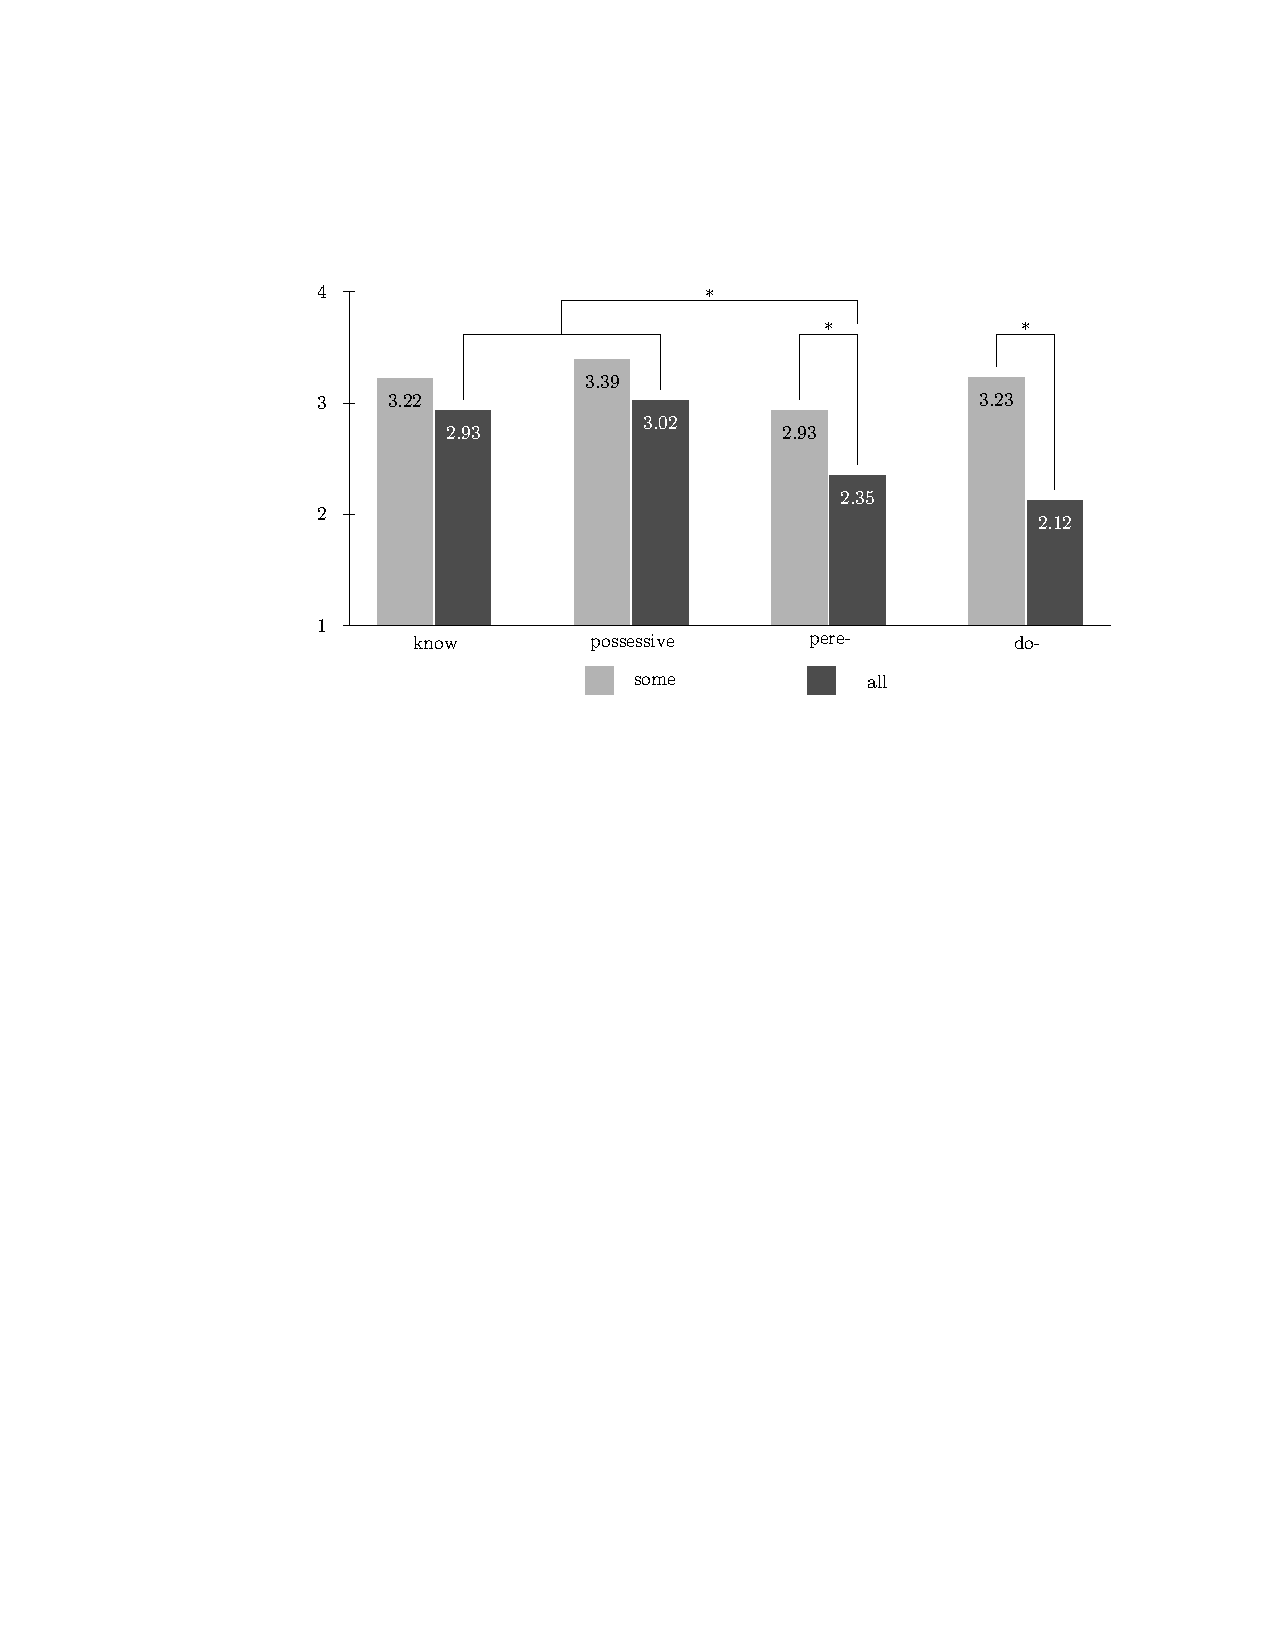
\includegraphics[width=\textwidth]{tr1.pdf}
\caption{Acceptability of existential and universal inferences for different triggers}
\label{fig:results}
\end{figure}

The main results of the questionnaire are provided in \figref{fig:results}.\footnote{Asterisks indicate significant difference.} It turned out that there is no statistically significant difference between the acceptance rates of \isi{universal and} existential inferences in case of the \isi{presupposition trigger} \textit{znat'} `to know' and posessive pronouns, which is in line with the results obtained in \citealt{Chemla:09}. There is, however, a statistically significant difference in the acceptance rate of \isi{universal and} existential inferences in case of test items of both categories: those involving the verb with the \isi{completive} prefix \Prefix{do-} and those with the verb prefixed with the iterative \Prefix{pere-} ($t$-test, $p<0.001$ in both cases). For the existential inferences, the answers ranged from ``yes'' to ``probably no'' and for the universal inferences, from ``probably yes'' to ``no'' and the overall results cannot be explained in terms of between-speaker variation. Furthermore, the difference between the acceptance rates in control and
test sentences for existential inferences was not significant, while the
difference for universal inferences was ($t$-test, $p<0.001$).

The obtained results strongly suggest that the inferences triggered by the \isi{completive} prefix \Prefix{do-} and the iterative prefix \Prefix{pere-} are not of a presuppositional nature. On the other hand, the observed behaviour is compatible with a scalar \is{implicatures}implicature analysis.

\subsection{Conclusion}
The standard tests for semantic and pragmatic presuppositions show that inferences triggered by the perfective aspect of accomplishments do not behave like semantic or pragmatic presuppositions.

As for the inferences triggered by prefixes \Prefix{do-} and \Prefix{pere-}, standard tests could not be used as evidence for or against presuppositional analysis, and therefore a new testing method is used to establish their nature: a questionnaire based on results of experimental work by \citet{Chemla:09}.
The \isi{projection properties} of Russian verbs containing prefixes \Prefix{do-} and \Prefix{pere-} in downward entailing contexts (under the \isi{universal quantifier} \textit{no}) indicate that the projected \isi{inference} behaves more like scalar \is{implicatures}implicature than like \isi{presupposition}.

%\subsection{Factual Imperfective}
%Write about \cite{Gronn:04}
%In the book \cite{Boguslawski:63} the author suggests that factual uses of imperfective are just the the reductions of the sentences with the corresponding perfective verb.

\section{The overall pragmatic picture}\label{section:pragm:overall}
In Chapter~\ref{Chapter5}, I have evoked the notion of the \isi{pragmatic competition} several times. In order to see how this competition works on the level of the whole \isi{prefixation} system to result in the global picture, let us look at the domain of verbal meanings and see how this domain is covered with prefixed verbs. I propose that whenever the general meaning of the prefix is underspecified, the interpretation of a particular verb gets settled in the optimal way for the range of the prefixed verbs derived from one root to cover the range of meanings a speaker may want to express. The reasoning that I outline below is a first sketch of the analysis that must be tested on a wider range of examples.

First let me illustrate the flexibility of the individual prefixes. As we have discussed in Sections~\ref{subsection:semantics:na} and \ref{subsection:semantics:po}, verbs prefixed with \Prefix{na-} or \Prefix{po-} can refer to events that culminate when the expected/\isi{standard degree} is reached. In addition, verbs prefixed with \Prefix{na-} can denote events that culminate at the degree higher than the expected degree. As for the verbs prefixed with \Prefix{po-}, they may refer to events that culminate without reaching the \isi{standard degree}. This part of the \isi{prefixation} system is complemented by the prefix \Prefix{pere-} that contributes the semantics of \isi{excess}. Let us consider the verbs prefixed with \Prefix{pere-} in its \isi{excessive} usage. It turns out that there is always another verb derived from the same base, that is used as a \isi{neutral perfective}. Under \textit{neutral perfective} I mean either a verb that refers to an action performed until the normal/standard/appropriate degree,\footnote{These verbs would constitute \isi{aspectual pairs} with the imperfective source verbs on the pair-based accounts of Russian verbal system. \citet{Janda:07a} calls such verbs Natural Perfectives. See also Chapter~\ref{Chapter2} for a discussion.} or a verb that denotes an action that lasted for some non-specified time.\footnote{Such verbs fall in the Complex Act Perfectives class in the account by \citet{Janda:07a}.} For example, if the verb \textit{gret'} `to heat' is prefixed with \Prefix{pere-}, the resulting verb \textit{peregret'} means `to overheat'. The same verb can be prefixed with \Prefix{na-} and the resulting verb \textit{nagret'} means `to warm up (until the desired temperature)'. In addition, the verb \textit{pogret'} `to heat' means warming up without necessarily reaching some particular temperature. In this case both \textit{nagret'} `to warm up'  and \textit{pogret'} `to heat' are \isi{neutral perfectives}, only with respect to different \isi{scales}. More pairs and triples are provided in the Table \ref{table:competition}. Let us explore them. 

\begin{sidewaystable}
\caption{Distribution of excess-denoting and neutral perfectives across verbal bases and prefixes \label{table:competition}}
\begin{tabularx}{\textwidth}{l  l  l  l  Q}
\lsptoprule
source verb& translation & ``\isi{excess}'' & neutral & other competing verbs\\ \midrule
\textit{zanimat'sja} & `to study' & \textit{perezanimat'sja} & \textit{pozanimat'sja} & \\
\textit{platit'} & `to pay' & \textit{pereplatit'} & \textit{zaplatit'} & \textit{oplatit'$_{\TR}$} `to pay for smth'\\
\textit{rabotat'} & `to work' & \textit{pererabotat'} & \textit{porabotat'} & \textit{otrabotat'$_{\TR}$} `to work in compensation of smth'\\

\tablevspace
\textit{xvalit'} & `to praise' & \textit{perexvalit'} & \textit{poxvalit'} &\\
\textit{\v{z}arit'} & `to fry' & \textit{pere\v{z}arit'} & \textit{po\v{z}arit'} & \textit{pro\v{z}arit'} `to fry thoroughly,' \textit{na\v{z}arit'} `to fry a lot of'\\ 

\tablevspace
\textit{gret'} & `to heat' & \textit{peregret'} & \textit{nagret'} & \textit{pogret'} `to heat,' \textit{progret'} `to heat through'\\ 
\textit{kormit'} & `to feed' & \textit{perekormit'} & \textit{nakormit'} & \textit{pokormit'} `to feed'\\
\textit{trenirovat'} & `to train' & \textit{peretrenirovat'} & \textit{natrenirovat'} & \textit{potrenirovat'} `to train for some time'\\\lspbottomrule
\end{tabularx}
\end{sidewaystable}

The upper third of the table contains three intransitive verbs. The prefix that is used to form a \isi{neutral perfective} depends on the scale lexicalised by the verb. If there is no scale except for the \isi{time scale}, the prefix \Prefix{po-} is used. If there is a scale that allows for the attachment of the \isi{resultative} \Prefix{za-}, it may be the option. The lines in the middle third of the table are occupied by two \isi{transitive verbs} that denote events that are by default measured according to these verbs' \isi{internal} \isi{scales} and do not rely on the information coming from the verbal arguments. These verbs form \isi{neutral perfectives} using the prefix \Prefix{po-}. In the bottom third the other type of \isi{transitive verbs} is represented: for those verbs the standard is determined for the pairs of event types and undergoers. In such case it is the \Prefix{na-}prefixed verb that refers to the situation of reaching the standard. The attachment of the prefix \Prefix{po-} is also possible, but now the \Prefix{po-}prefixed verbs tend to refer to events in course of which the standard value is not reached.

What we see is that even if the range of prefixes that two verbs can attach is the same, as for the verbs \textit{\v{z}arit'} `to fry' and \textit{gret'} `to heat', the semantic contribution of these prefixes may be different. While both \textit{pere\v{z}arit'} `to burn by frying' and \textit{peregret'} `to overheat' have the meaning of \isi{excess}, the role of the prefix \Prefix{na-} in the verbs \textit{na\v{z}arit'} `to fry a lot of' and \textit{nagret'} `to heat' seems to be not the same. In what follows we will explore a couple of verbs in detail and see how these differences in the final semantic contribution can be explained using \isi{pragmatic competition} principles.

Consider the verb \textit{zimovat'} `to spend the winter'. The OSLIN database of verbal aspect provides the following list of the verbs derived from it: \textit{vyzimovat'} `to survive the winter' (usually about the plants), \textit{dozimovat'} `to spend the rest of the winter', \textit{zazimovat'} `to stay for the winter', \textit{otzimovat'} `to finish spending the winter', \textit{perezimovat'} `to spend the winter', \textit{pozimovat'} `to spend some winter time', \textit{prozimovat'} `to spend the winter time'. Examples illustrating the usage of these verbs are provided in \ref{ex:zimovat'}.

\ex.\label{ex:zimovat'}\ag.\label{ex:vyzimovat'}Vinograd ne mo\v{z}et vyzimovat' v srednej polose RSFSR.\\
grape not can.\glb{pres.sg.3} vy.winter.\glb{inf} in middle band RSFSR\\
\trans `Grape cannot survive the winter in the midland of the RSFSR.'\\\Source{= example of verb usage from \citealt{Ushakov:50}}
\bg.\label{ex:dozimovat'}Dozimuem na korable vo l'dax.\\
do.winter.\glb{pres.pl.1} on ship in ice.\glb{pl.prep}\\
\trans `We will spend the rest of the winter on a ship on the ice.'\\\Source{= example of verb usage from \citealt{Ushakov:50}}
\bg.\label{ex:zazimovat'}\`{E}kspedicija zazimovala na Novoj Zemle.\\
expedition.\glb{sg.nom} za.winter.\glb{pst.sg.f} on Novaya Zemlya\\
\trans `The expedition wintered on Novaya Zemlya.'\\\Source{= example of verb usage from \citealt{Ushakov:50}}
\bg.\label{ex:otzimovat'}Otzimovali my pervuju zimu, k vesne priez\v{z}aet Matvei\v{c}.\\
ot.winter.\glb{pst.pl} we first winter.\glb{sg.acc}, to spring pri.ride.\glb{pres.sg.3} Matveich\\
\trans `We have spent the first winter, Matveich will arrive when the spring comes.'\Source{Dmitrij Karalis. \textit{Roman s geroinej} (2001)}
\bg.\label{ex:perezimovat'}Perezimovat' v derevne.\\
pere.winter.\glb{inf} in village.\glb{sg.prep}\\
\trans `To spend the winter in a village.'\\\Source{= example of verb usage from \citealt{Ushakov:50}}
\bg.\label{ex:pozimovat'}Ix by k nam na severa, \v{c}toby pozimovali v svoix karto\v{c}nyx domikax.\\
they {} to us on north.\glb{pl.prep}, that po.winter.\glb{pst.pl} in their card house.\glb{pl.prep}\\
\trans `I would like to see them spending winter time here in the north in their houses of cards.'\Source{\url{doskapozorakomi.ru}}
\bg.\label{ex:prozimovat'}Po oby\v{c}aju togo vremeni polk na\v{s} prozimoval v odnix i tex \v{z}e kvartirax osem' zim s li\v{s}kom.\\
along custom that time regiment.\glb{sg.nom} our pro.winter.\glb{pst.sg.m} in one and that same flat.\glb{pl.prep} eight winters with over\\
\trans `According to the customs of that time our regiment spent a bit more than eight winters in the same flats.'\\\Source{T. G. \v{S}ev\v{c}enko. \textit{Kapitan\v{s}a} (1855)}

The abundance of the derivatives of the verb \textit{zimovat'} `to spend the winter' that one finds in the dictionary data, turns out to be undermined by the status of some of these verbs in the contemporary language. Two verbs from this list are barely used (\textit{vyzimovat'} `to survive the winter' and \textit{otzimovat'} `to finish spending the winter'), the verb \textit{prozimovat'} `to spend the winter time' has been used but is not common any longer (corpora examples are mostly dated with the XIX century), so we are left with four verbs that are actually encountered in text and speech: \textit{zazimovat'} that refers to the beginning of the `spending the winter' event, \textit{dozimovat'} that focuses on its end, \textit{perezimovat'} that denotes spending the time of the whole winter, and \textit{pozimovat'} that is not related to a specific portion of the winter, but to any amount of the winter time (can be part of one winter or multiple winters). With these four verbs, we see how the available prefixed verbs cover the domain of fixing different set of points: \textit{pozimovat'} `to spend some winter time' describes a finished event of staying in some particular place without imposing further restrictions on the start and the end of the stay; \textit{zazimovat'} `to stay for the winter' establishes a connection between the start of a stay in one place and the beginning of the winter; \textit{dozimovat'} `to spend the rest of the winter' fixes the end point of the stay to be related to the end of the winter; \textit{perezimovat'} `to spend the winter' relates both the start and the end points of the stay to the beginning and the end of the winter, respectively.

The question I want to answer here is why, for example, the verb \textit{pozimovat'} `to spend some winter time', that contains the prefix \Prefix{po-} and therefore could, from the semantics point of view, mean `to spend the whole winter', is usually not used to refer to such an event. Similarly, the verb \textit{dozimovat'} `to spend the rest of the winter' is also not used to refer to the situation of spending the whole winter despite the fact that there is no \isi{semantic restriction} that would prevent it. To see how the distribution of the meanings gets established, let us first represent the different logically natural meanings that can be realised by means of the prefixed verbs. 

It is reasonable to assume that if the speaker wants to refer to a completed event of spending some winter time at a particular location, there are in principle four situations that they may want to describe (as there are only two distinguished points on the \isi{time scale} in this case): the situation of spending one whole winter, the situation of spending the initial part of the winter, the situation of spending the final part of the winter, and the situation of spending some time of the winter without bounding the event \isi{duration} to the \isi{duration} of the winter. These four situations are presented in Table~\ref{table:zimovat}.

\begin{table}
\caption{The domain of terminated events related to spending the winter \label{table:zimovat}}
\begin{tabular}{lcc}
\lsptoprule
 & event start = winter start & event end = winter end\\
\midrule
t$_1$ & + & +\\
t$_2$ & + & \textminus\\
t$_3$ & \textminus & +\\
t$_4$ & \textminus & \textminus\\
\lspbottomrule
\end{tabular}
\end{table}

Now let us see which prefixed verbs can describe which of the situations t$_1$--t$_4$ given the restrictions in the semantics of these prefixes. As we have discussed before, for the prefix \Prefix{pere-} this will be the equation of both event start and event end to the start and the end points of the relevant scale. The prefix \Prefix{za-} necessarily equates the start point of the event with the start point of the scale, the prefix \Prefix{do-} only fixes the end point of the event, equating it with the end point of the relevant scale. The prefix \Prefix{po-}, in turn, does not restrict the positions of the start and the end points of the event with respect to the scale. In our case the scale in question is the \isi{time scale} with the start and the end points associated with the start and the end of the winter.  The combination of the meanings specified in Table~\ref{table:zimovat} with the restrictions imposed by particular prefixes is shown in \figref{fig:zimovat}.

\begin{figure}
\centering
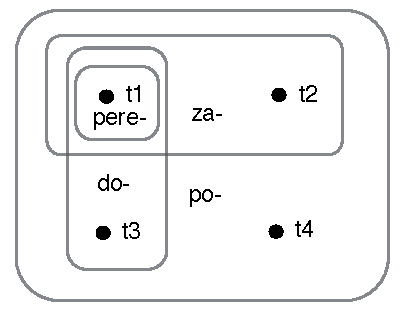
\includegraphics[scale=0.8]{dia-zimovat.pdf}
\caption{Possible interpretations of the verbs derived from \textit{zimovat'} `to spend the winter', see also Table~\ref{table:zimovat} \label{fig:zimovat}}
\end{figure}

Now pragmatic theory (e.g., \isi{Optimality Theory}, henceforth \isi{OT}, see \citealt{Blutner:00, vanRooy:04, Benz:11}) can be applied to the underspecified semantics representations of the prefixed \isi{perfective verbs} derived from the base verb \textit{zimovat'} `to spend the winter'. As is shown in \figref{fig:zimovat}, the optimal usage of prefixed verbs would be to describe t$_1$ with the verb \textit{perezimovat'} `to spend the winter', t$_2$ and t$_3$ -- with the verbs \textit{zazimovat'} `to stay for the winter' and \textit{dozimovat'} `to spend the rest of the winter', respectively. The verb \textit{pozimovat'} `to spend some winter time' is then used in the situation t$_4$, but not in the other cases. This is exactly the distribution that is observed in the data. 

The case of the verbs that refer to the \isi{time scale} only is in a way the simplest, as there are no other \isi{scales} intervening. Let us now consider the verb \textit{gret'} `to heat' that is also part of Table~\ref{table:competition}. The default scale for this verb is the temperature scale. The distinguished point on this scale is the desired/appropriate temperature (let us call is t$_s$). Temperature t$_s$ depends on the direct object, as the verb \textit{gret'} `to heat' is transitive. It is also possible to talk about the other point on the scale that represents the temperature of the object at the start of the heating event, but it is not relevant for determining the space of meanings. With this we obtain three possible meanings related to the temperature scale that one may want to express: reaching a point below the distinguished point, reaching exactly the distinguished point, and reaching some point above the distinguished point. Let us call the temperature reached by the end of the heating event t$_f$. The space of meanings is presented in Table~\ref{table:gret}.

\begin{table}
\caption{The domain of terminated events related to heating \label{table:gret}}
\begin{tabular}{lccc}
\lsptoprule
 & t$_f$ $>$ t$_s$ & t$_f$ = t$_f$ & t$_f$ $<$ t$_f$\\
\midrule
t$_1$ & 1 & 0 & 0\\
t$_2$ & 0 & 1 & 0\\
t$_3$ & 0 & 0 & 1\\
\lspbottomrule
\end{tabular}
\end{table}

\begin{figure}
\centering
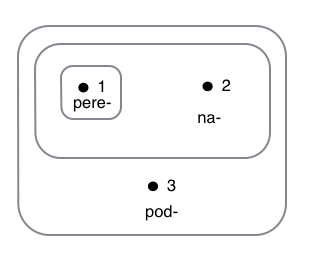
\includegraphics[scale=0.5]{dia-gret.png}
\caption{Possible interpretations of the verbs derived from \textit{gret'} `to heat', see also Table~\ref{table:gret} \label{fig:gret}}
\end{figure}

What we see in \figref{fig:gret} is the range of the meanings that certain prefixed verbs derived from the verb \textit{gret'} `to heat' may cover given the general restrictions for the semantics of these prefixes. In particular, the verb \textit{peregret'} `to overheat' can refer only to the situation of heating the object more than up to t$_s$. The verb \textit{nagret'} `to warm up' could refer to the same situation as well as to heating exactly up to the expected temperature (this temperature can be also specified via a measure phrase). The verb \textit{podogret'} `to heat to some degree' that contains the prefix \Prefix{pod-} (not discussed in details in this work) can refer to an event of heating that terminates with a temperature being lower than t$_s$. The verb \textit{pogret'} `to heat' can refer to any event of heating.

Applying \isi{OT} to the verb-meaning pairs represented by \figref{fig:gret} results in the prediction that in the situation of overheating the verb \textit{peregret'} `to overheat' should be used. In the situation of reaching the t$_s$ the appropriate description is provided by the verb \textit{nagret'} `to heat'. The verb \textit{podogret'} `to heat to some degree' denotes exactly the situations when the temperature reached at the end of the heating event is below t$_s$. As all the relevant scenarios are covered by more specific verbs, the verb \textit{pogret'} `to heat' is used when the degree of change is not at issue and thus it is a \isi{neutral perfective}.

Taking just two verbs \textit{zimovat'} `to spend the winter' and \textit{gret'} `to heat' as examples already allows us to see the source of the observed \isi{variability of} the prefix interpretations. As a part of the verb \textit{pozimovat'} `to spend some winter time', the prefix \Prefix{po-} tends to be interpreted as restricting the portion of the winter time to be below the standard (where the standard is the \isi{duration} of the winter). As a part of the verb \textit{pogret'} `to heat' the same prefix does not restrict the \isi{duration} of the heating event, and the resulting verb often refers to an event of heating for the standard time. 

The description of the \isi{pragmatic competition} I offer here is a first sketch. It works nicely in a number of cases I explored, but it must be tested on a wider range of verbs. Further elaboration of the approach as well as answering questions related to such architecture of the analysis goes beyond the scope of this thesis. There is a hope that the preliminary analysis I proposed here can be implemented using the computational pragmatics approach of Rational Speech Act Theory (RSA, \citealt{Franke:09, FrankGoodman:12, GoodmanStuhlmuller:13, FrankeJager:15, GoodmanFrank:16}). 

One more question that I want to mention is whether the reasoning that is used to find an optimal distribution of meanings among the available verbs is computed online or is conventionalised. The account outlined here does not favour one of the views on this process, although the status of the semantic representations for prefixes depends on the answer to this question. In \isi{future} work, I plan to experimentally test whether speakers operate with the underspecified semantic representations or with conventionalised representations. 

\section{Summary}
In this chapter, we have explored inferences associated with perfective aspect and prefixes \Prefix{do-} and \Prefix{pere-}. I have provided tests that address the claim about the presence of the presuppositional component within all \isi{perfective verbs} and within verbs that are derived by prefixes \Prefix{do-} and \Prefix{pere-}. For the whole class of perfectives the standard tests were enough to show that the \isi{inference} in question does not have the presuppositional nature. In order to test whether prefixes \Prefix{do-} and \Prefix{pere-} trigger presuppositions I had to use a specially developed questionnaire. I then concluded that the observed inferences are better analysed as entailments and (scalar) \isi{implicatures} (in positive and negative environments, respectively) then as presuppositions.

In the second part of the chapter, I have proposed a preliminary analysis in terms of \isi{Optimality Theory} of how the \isi{prefixation} system in Russian works as a whole. The idea that I plan to develop in \isi{future} work is that the exact interpretation of the given verb depends on the range of competing verbs derived from the same base, while the semantic representation remains underspecified. The set of competing verbs in turn depends on the type of the scale the verb is associated with.

%\textit{igrat'} `to play.' This verb is not limited exclusively by the \isi{time scale}, the other natural domain is the outcome of the playing, but the time-related domain of meanings is richer. When this verb is used intransitively, there are no specific distinguished points on the \isi{time scale}, as in the case of the verb \textit{zimovat'} `to spend winter time.' The presence of a subject can contribute the appropriate time for the   \textit{pereigrat'} `to play for too long' refers to exceeding the time of playing appropriate for the subject. Together with the verbs \textit{poigrat'} `to play for some time' and \textit{proigrat' (3 \v{c}asa)} `to play continuously (for 3 hours)' the verb \textit{pereigrat'} `to play for too long' covers the domain of possible time-related meanings a speaker may want to express.

%\citet[516]{vanRooy:04} ``a linguistic convention can be seen as a behavioral phenomenon that developed through the forces of evolution.'' ``A strategy pair is successful when (i) it accounts for successful communication, and (ii) it does so with small effort.''

%TODO: bidirectional optimality theory
%TODO: Horn's division

%\section{Consequences of the proposed analysis}
%
%An important consequence of the analysis presented here is that by introducing the \isi{neutral perfectives} as verbs that take as start and end points either arbitrary points on the scale or the end points of the scale, we have sold the problem of so-called ``purely perfectivizing prefixes'' \textit{(\v{c}istovidovyje pristavki)}. Such prefixes, according to Russian academic dictionaries and grammars, lack the meaning and serve just to change the aspect of the verb. is now a topic of an ungoing debate. For traditional approaches, the existence of such prefixes is a natural result of a standard procedure of identifying the meaning when writing a dictionary or grammar article: the common difference between a \isi{series of} prefixed verbs versus \isi{unprefixed verbs} is considered to be the meaning of the prefix.
%
%from \citet{JandaNesset:10}:\\
%The idea of “empty” prefixes, also known as “purely aspectual /
%чистовидовые”, has a long tradition in Russian linguistics (Shaxmatov:52;
%Avilova:59, Avilova:76; Tixonov:64, Tixonov:98; Forsyth:70; Vinogradov:72; Shvedova82; Certkova:96; ZaliznjakShmelev:00; Mironova:	04). 
%Some scholars have
%objected to the concept of “empty” prefixes, hypothesizing instead that there
%is conceptual overlap between prefixes and base verbs (Vey:52; vanSchooneveld:58; Isachenko:60; Timberlake:04 410–11). Though this “overlap hypothesis” is an
%attractive solution, actually proving that the prefixes are not empty has turned
%out to be one of the most long-standing and intractable problems in the field;
%Krongauz:82 labels it a “chronic” problem lacking a satisfactory solution.
%
%Natural Perfectives have the same meaning as the corresponding unprefixed
%base verb, such as растаять ‘melt’ (cf. base verb таять ‘melt’) and
%распухнуть ‘swell’ (cf. base verb пухнуть ‘swell’). Svenonius (2004a–b) and
%Ramchand (2004) refer to prefixes in such perfectives as “purely perfectivizing
%prefixes”, a term that comports well with the traditional label of
%“чистовидовая приставка.”
%
%\begin{itemize}
%\item ``Expectation 1: If the prefixes in Natural Perfectives are empty, we expect
%there to be one such prefix. '' ``Russian has, however, at least sixteen prefixes that form Natural Perfectives.'' both on p. 482
%\item Expectation 2: If the prefixes in Natural Perfectives are empty, we expect the
%prefixes to be distributed randomly. p. 482 And this is not so
%\item Expectation 3: If the prefixes in Natural Perfectives are empty, we expect the
%distribution of prefix variation to be random.
%\item Expectation 4: If the prefixes in Natural Perfectives are empty, we expect
%their assignment to borrowed verbs to be random.
%\item Expectation 5: If the prefixes in Natural Perfectives are empty, we expect
%them to stay empty.
%\end{itemize}
%
%Semantic overlap functions as a kind of camouflage making
%the meaning of the prefix hard to distinguish because it is included in the
%meaning of the verb. p. 487
%
%---------------\\
%from \citet[212]{Janda:13}
%This article focuses on the use of prefixes to form “purely aspec-­‐‑
%tual” perfective partners to simplex \isi{imperfective verbs}. Prefixes used
%for this purpose are claimed by many scholars to be devoid of meaning
%(beyond marking the verb as perfective) and thus semantically “emp-­‐‑
%ty” (Šaxmatov 1952, Avilova 1959 and 1976, Tixonov 1964 and 1998,
%Forsyth 1970, Vinogradov 1972, Švedova et al. 1980, Čertkova 1996,
%Zaliznjak and Šmelev 2000, Mironova 2004). The view that prefixes are
%“empty” when they serve the function of creating \isi{aspectual pairs} rests
%upon a logical argument in which we assume that meanings are like
%mathematical values. Thus if “m” is the lexical meaning of a simplex
%verb “s”, we can assume that m = s (for example, ‘write’ = pisat’). If we
%perfectivize “s” by adding a prefix “p”, the result, it is claimed, is a
%perfective verb that has the same lexical meaning as “s”, so m = p + s
%(‘write’ = napisat’). Since both “s” and “p + s” equal “m”, the value of
%“p” by this logic is necessarily zero. In other words, the prefix has no
%meaning because the lexical meaning of the verb is not changed when
%it is added. All the prefix adds is the grammatical value “+ perfective”,
%but that does not change the lexical meaning of the verb.
%
%alternative model, according to which the prefixes do bear meaning even
%when they are used to create \isi{aspectual pairs} (Vey 1952, van Schoon-­‐‑
%eveld 1958, Isačenko 1960, Timberlake 2004: 410–11). Under this alter-­‐‑
%native model, it is hypothesized that the meanings of the prefixes
%overlap with the meanings of the simplex verbs. For example, one
%could say that the prefix \isi{na-}­‐‑ is associated with accumulation on a sur-­‐‑
%face, and pisat’ ‘write’ is about accumulating symbols on a surface,
%motivating napisat’ ‘write’. Conceptual overlap works like camouflage,
%creating the illusion that the prefix is “empty” even though it is not.
%
%\citet{Janda:07b} suggests the term “Natural Perfectives” for verbs
%formed with “purely perfectivizing” prefixes, “Specialized Perfec-­‐‑
%tives” for verbs formed with “lexical” prefixes, and “Complex Act Per-­‐‑
%fectives” for verbs formed with “super-­‐‑lexical” prefixes.
%Janda addi-­‐‑
%tionally identifies “Single Act Perfectives” with a \isi{semelfactive} mean-­‐‑
%ing (such as čixnut’ ‘sneeze once’) and shows that the types of perfec-­‐‑
%tives have distinct tendencies in terms of their semantics and deriva-­‐‑
%tional behavior.
%
%Whereas Specialized Perfectives nearly always form
%secondary imperfectives, this type of derivation is resisted to various
%degrees by the other types of perfectives. Natural Perfectives and Spe-­‐‑
%cialized Perfectives usually refer to actions that have a natural culmi-­‐‑
%nation (the completion of a document for napisat’ ‘write’ or a revision
%for perepisat’ ‘rewrite’); by contrast, Complex Act Perfectives and Sin-­‐‑
%gle Act Perfectives usually refer to actions that lack a sense of complet-­‐‑
%ability (popisat’ ‘write for a while’ is about writing without an inherent
%telos, and the lack of a culmination is inherent in sneezing as we see in
%počixat’ ‘sneeze for a while’ and čixnut’ ‘sneeze once’). Natural Perfec-­‐‑
%tives tend to behave like a closed-­‐‑class category, with a limited type
%frequency (under 2,000 verbs; see below) and relatively high token fre-­‐‑
%quency (the average median frequency of a Natural Perfective in the
%Russian National Corpus is 107), whereas other perfectives are an
%open class with unlimited type frequency (permitting occasionalisms)
%and relatively low token frequency (average median token frequency
%9.7; cf. Kuznetsova 2010). Admittedly there is no perfect dividing line
%between Natural Perfectives and other perfectives. However, there are
%very strong tendencies in this system, and the case of most verbs is
%clear despite the existence of some controversial examples.
%
%\citet[16-18]{Janda:11}
%The \isi{cluster model} elaborates on the pair model in that pairs, where they exist, are either a type of cluster structure, or, more frequently, pairs are embedded in larger cluster structures containing multiple types of perfectives. In addition, the \isi{cluster model} allows for structures that do not contain pairs at all. Overall, the \isi{cluster model} is more accurate than the pair model in that it provides a comprehensive account of the real complexity of the Russian aspect system. 
%
%Crucial to the \isi{cluster model} is the recognition of four major types of perfectives, based on their semantics and morphological behavior. The main division between the types of perfectives is motivated by Completability, since two types of perfectives are Completable and two are Non-Completable. The four types of perfectives are presented here, along with their Completability status and descriptions of the morphological behavior associated with each type:
%Natural Perfectives like napisat’ ‘write’ and svjazat’ ‘tie’ generally correspond to the perfective partners of \isi{imperfective verbs} according to the pair model and share the same lexical meaning as their imperfective correlates pisat’ ‘write’ and vjazat’ ‘tie’. Natural Perfectives are strongly Completable, since they refer to the natural conclusion of a goal-oriented situation. Most Natural Perfectives are formed via \isi{prefixation} of base \isi{imperfective verbs}, and such Natural Perfectives often resist the formation of secondary imperfectives. Natural Perfectives can be formed from imperfectives that are either strongly Completable themselves (cf. perfective okrepnut’ from krepnut’ ‘get stronger’) or are ambiguous as to Completability (cf. perfective napisat’ from pisat’ ‘write’). There are a few base \isi{perfective verbs}, usually referring to \isi{punctual events} such as dat’ ‘give’ that serve as Natural Perfectives and derive the corresponding imperfective via \isi{suffixation}, as in davat’ ‘give’. In addition, there are non-prototypical morphological relationships between Natural Perfectives and corresponding imperfectives, including \isi{homonymy} (with bi-aspectual verbs like likvidirovat’ ‘liquidate’, where one form is both perfective and imperfective), suppletion (e.g., skazat’ ‘say’ perfective and govorit’ ‘say’ imperfective), and semi-suppletion (e.g., brosit’ ‘throw’ perfective and brosat’ ‘throw’ imperfective). 
%Specialized Perfectives like perepisat’ ‘revise’ and razvjazat’ ‘untie’ are lexically distinct from their corresponding base verbs because the prefixes direct the action in a way not inherent in the base verb. Specialized Perfectives are strongly Completable, for they refer to situations that are goal-oriented and conclude with a result (a revised manuscript or an untied knot). Specialized Perfectives can be formed from all three types of imperfectives: Completable imperfectives (such as blokirovat’ ‘block’ which forms razblokirovat’ ‘unblock’), ambiguous imperfectives (such as pisat’ ‘write’, which forms perepisat’ ‘revise’), and Non-Completable imperfectives (such as rabotat’, which forms pererabotat’ ‘revise’). There are, however, some Non-Completable imperfectives that cannot form Specialized Perfectives (such as stonat’ ‘moan’). Unlike Natural Perfectives, Specialized Perfectives nearly always form secondary imperfectives (such as perepisyvat’ ‘revise’ and razvjazyvat’ ‘untie’; but note that some verb stems resist the formation of any \isi{secondary imperfective}, like kipjatit’ ‘boil’, which forms no \isi{secondary imperfective} from Specialized Perfectives like perekipjatit’ ‘overboil’). 
%Complex Act Perfectives like postonat’ ‘moan for a while’ or zaprygat’ ‘start hopping’ quantize engagement in an action that lacks goal-directedness. Complex Act Perfectives focus on starting (ingressives) or stopping (terminatives) an activity or engaging in an activity for a while (delimitatives and perduratives). Since Complex Act Perfectives entail neither progress nor a result, they are strongly Non-Completable. Only imperfective base verbs that have a Non-Completable construal can form Complex Act Perfectives. Thus base verbs that are either Non-Completable (like stonat’ ‘moan’) or ambiguous for Completability (like čitat’ ‘read’) can form Complex Act Perfectives (postonat’ ‘moan for a while’ and počitat’ ‘read’ for a while), whereas strongly Completable base imperfectives tend not to form Complex Act Perfectives (such perfectives are not formed from verbs like krepnut’ ‘get stronger’ and likvidirovat’ ‘liquidate’). Complex Act Perfectives are formed by means of \isi{prefixation} (primarily \isi{po-}, \isi{pro-}, and \isi{za-}, though other prefixes such as \isi{ot-}, \isi{raz-} and \isi{na-} also appear), and strongly resist the formation of secondary imperfectives.
%
%---------------
%
%
%However, many linguists argue against such approach and explain the fact that the meaning of such prefixes cannot be extracted not because it is not present in the prefix, but because it is also a part of the meaning contributed by the stem. This approach is advanced in such works as \cite{Isachenko:60}, \cite{Filip:00}, \cite{JandaNesset:10} and others.
%
%``the meaning of the base verb and
%prefix overlap, rendering the contribution of the prefix redundant. Redundancy,
%however, is not the same as emptiness.'' -- \citet{JandaNesset:10}
%
%
%So in addition to proposing a unified treatment for various usages of certain prefixes I want to push forward the idea of viewing the \isi{polysemy} of prefix contributions as a tool for covering the domain of meanings speakers may want to express. This is in some way resembling the proposal of \citet{Janda:07a}, who subdivides \isi{perfective verbs} into Natural, Complex Act, Single Act and Specialized Perfectives and then explores whether there is a certain order in which those classes get populated. As I have already noted above, some of those verbs that I classify as \isi{neutral perfectives} are Natural Perfectives and some are Complex Act perfectives in the theory of \citet{Janda:07a}. For me it is important to unify those verbs in one category because this allows to see that additional inferences occur exactly in those situation when there are several prefixed verbs that could play this role.

%In section \ref{sec:pres:against}, we apply the classical tests for semantic and pragmatic \isi{presupposition} to Russian data. We show that the hypothesis about the presuppositional nature of the \isi{inference} triggered by \isi{perfective verbs} is only applicable to a subset of perfective predicates, namely perfective accomplishments, rather than to perfectives as a whole class. Moreover,we show that this hypothesis must be rejected. When it comes to the prefixes \Prefix{do-} and \Prefix{pere-}, the tests prove to be insufficient because they do not lead to any clear judgments on the part of native speakers. In section \ref{proposal}, we present our proposal and motivate its plausibility. Section \ref{empirical} is devoted to the online questionnaire we conducted, which provides empirical evidence which supports our proposal in section \ref{proposal}.
 % Pragmatics
% Chapter 7

\chapter{Frame semantics for prefixes} % Write in your own chapter title
\label{Chapter7}
%\lhead{Chapter 6. \emph{Frame semantics for prefixes}} 

As I have shown in the previous chapters, Russian verbal prefixation is a complex system that cannot be successfully modelled by means of one linguistic layer. In order to simplify individual components of the system and allow for the observed flexibility without massive overgeneration, one needs to coordinate the work of the morphological, syntactic, semantic, and pragmatic representations, as well as describe the interfaces between them. In the fragment I describe here I limit myself to the first three systems, leaving pragmatic strengthening at the level of a tentative proposal provided in Chapter~\ref{Chapter6}. Even with this limitation there are not a lot of formalisms that would be suitable for such a representation.

Following \citet{KallmeyerOsswald:12, KallmeyerOsswald:13}, I will adopt a combination of frame semantics \citep{Fillmore:82} and Lexicalized Tree Adjoining Grammars (LTAG, \citealt{JoshiSchabes:97}, \citealt{Frank:92}, \citealt{AbeilleRambow:00}, \citealt{Abeille:02}, \citealt{Frank:02}). This framework has various benefits, such as a transparent syntax-semantics interface, numerous factorisation possibilities within the lexicon (especially important for modelling of the derivational morphology), and cognitive plausibility. More information about the advantages of frame-based LTAG semantics can be found in \citet{KallmeyerOsswald:13}. 

In this chapter, I concentrate on the semantic side of the analysis and show semantic composition that is triggered by operations at the morphological and syntactic levels. I also provide trees and tree fragments that are associated with the proposed semantic frames, but the presentation is kept on a level suitable also for those readers that are not familiar with LTAG and XMG 2 \citep{Petitjean:16}. In Chapter~\ref{Chapter8} I will provide more technical details about the syntactic part of the analysis, metagrammar decomposition, and specific implementation problems. As for the material that I present in this chapter, the number of decisions motivated by the framework restrictions is small and I discuss all of them. Thus, the proposed frames can be easily adapted to be used within some other framework or even translated into another language of semantic description, e.g. Neo-Davidsonian event representation.

\section{LTAG and frame semantics}
\subsection{TAG}\label{section:tag}
Tree Adjoining Grammar (TAG, \citealt{JoshiSchabes:97}, \citealt{AbeilleRambow:00}) is a tree-rewriting grammar formalism. A TAG consists of a finite set of \textit{elementary trees} with labelled nodes with two operations on them: \textit{substitution} and \textit{adjunction}. 

All elementary trees are either \textit{auxiliary trees} or \textit{initial trees}. An \textit{auxiliary tree} is a tree which has exactly one \textit{foot node} -- a leaf that is marked with an asterisk. Leaf nodes can be labelled with terminals and other nodes are labelled only with non-terminals. The derivation process starts from an initial tree and in the final \textit{derived tree} all the leaves must be labelled by terminals.

Substitution allows to replace a non-terminal leaf with a new tree and adjunction is used for replacing an internal node with an auxiliary tree. Adjunction to the node labelled with X is allowed if the root and foot nodes of the adjoining auxiliary tree have the same label X. It is also possible to indicate nodes where adjunction is obligatory or not allowed and to specify the set of all possible trees for adjunction.

Figure \ref{fig:exampletree} shows an example of a derivation: the initial tree for \textit{Mary} substitutes into the subject slot of the elementary tree for \textit{laughs}, and the \textit{sometimes} auxiliary tree for the VP modifier adjoins to the VP node. The result of performing these two operations is shown on the right side of the same figure.

\begin{figure}[h!]
	\centering
	\hspace{-0.6cm}    
    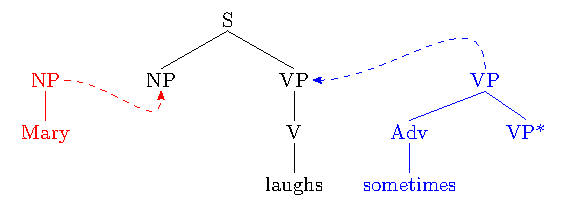
\includegraphics[width=8cm]{treeMaryLaughs.pdf} 
    \hspace{0.4cm}
    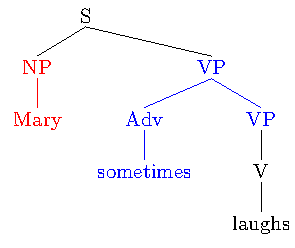
\includegraphics[width=4cm]{derivedTreeMaryLaughs.pdf} 
    \caption{Example of a TAG derivation}
    \label{fig:exampletree}
\end{figure}

\paragraph*{Feature-structure based TAG} Feature-structure based TAG, or FTAG, is a variant of TAG in which elementary trees are enriched with feature structures \citep{Vijay-ShankerJoshi:88}. Using feature structures as non-terminal nodes allows to generalize agreement via underspecification, helps to model adjunction constraints and leads to more compact grammars.

For example, \figref{fig:nofstruct} shows the derivation of the sentence \textit{``Grammars leak"} without feature structures and some trees involved in it (this example, including the \figref{fig:nofstruct},  \figref{fig:grleaksubst},  \figref{fig:isleaking}, and  \figref{fig:isleakingresult}, is due to Timm Lichte). One can see that already such a small piece of derivation contains a lot of redundancy that cannot be avoided if only labelled categories are used. In such a TAG, the following trees have to be kept in the grammar for a regular noun, such as \textit{grammars}: third person singular nominative, third person singular accusative, plural nominative, and plural accusative.
\begin{figure}[h!]
	\centering
    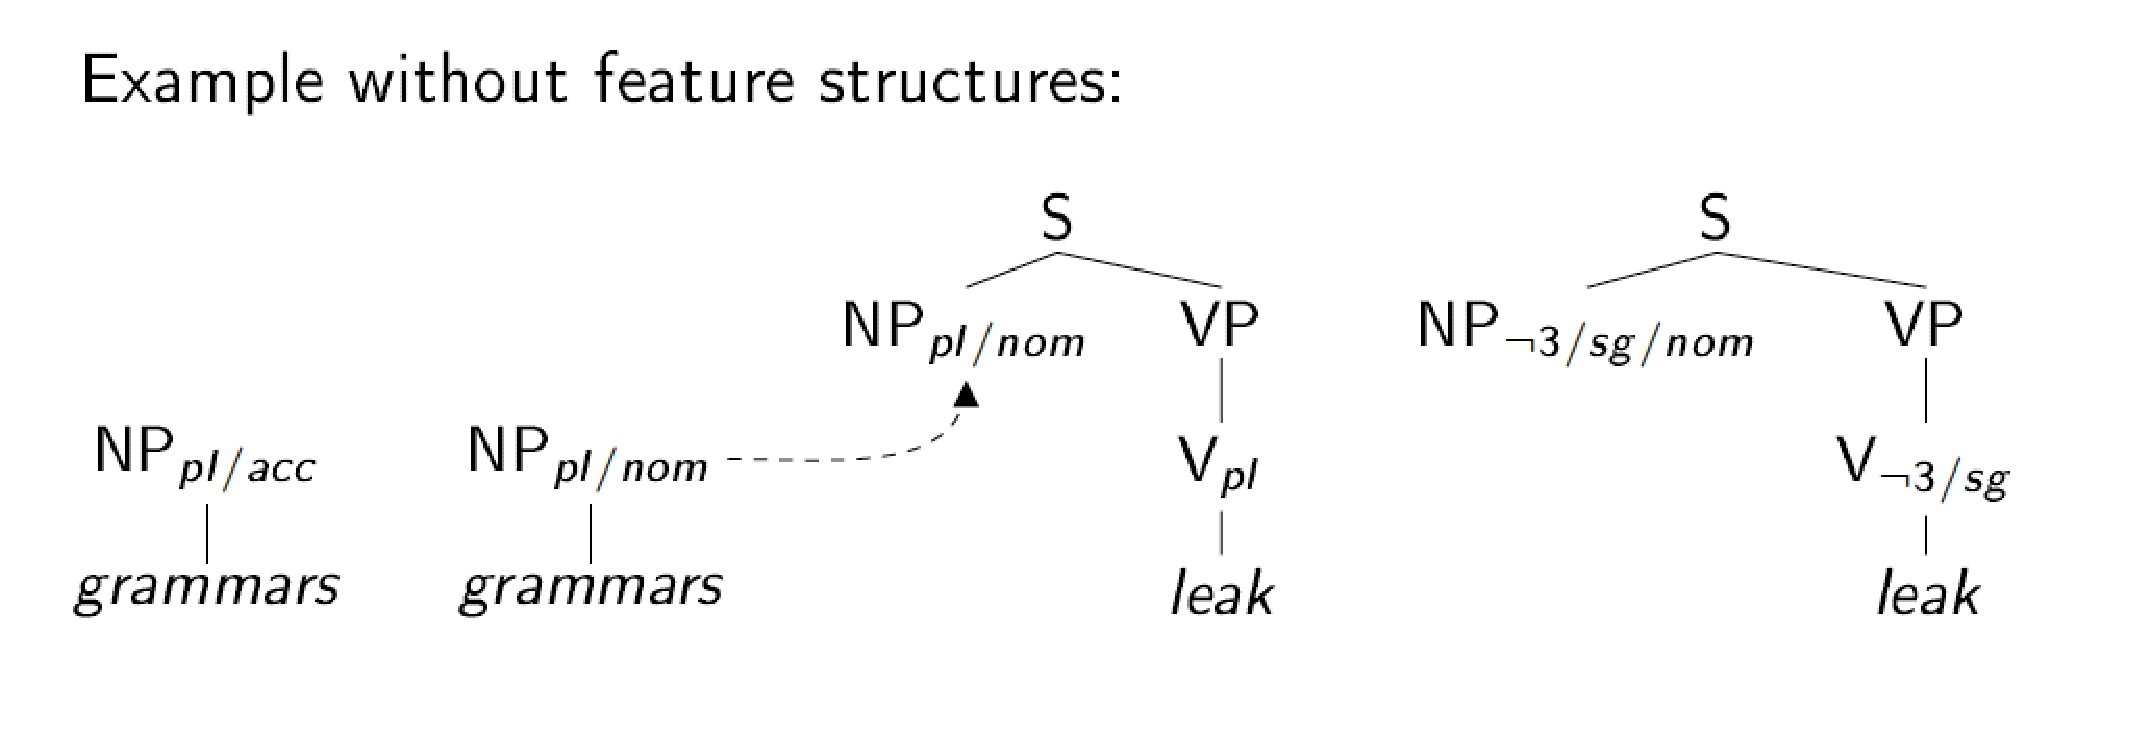
\includegraphics[scale=0.35]{nofstruct.pdf}
    \caption{Example of a derivation for \textit{``Grammars leak"} without feature structures  \label{fig:nofstruct}}
\end{figure}

If feature structures are used, the example described above looks as shown on \figref{fig:grleaksubst}. In this case only two entries for the noun \textit{grammar} must be kept in the lexicon: one for the single form \textit{grammar} and one for the plural form \textit{grammars}. Case can remain underspecified, as it does not influence the surface form of the noun.

\begin{figure}[h!]
	\centering
    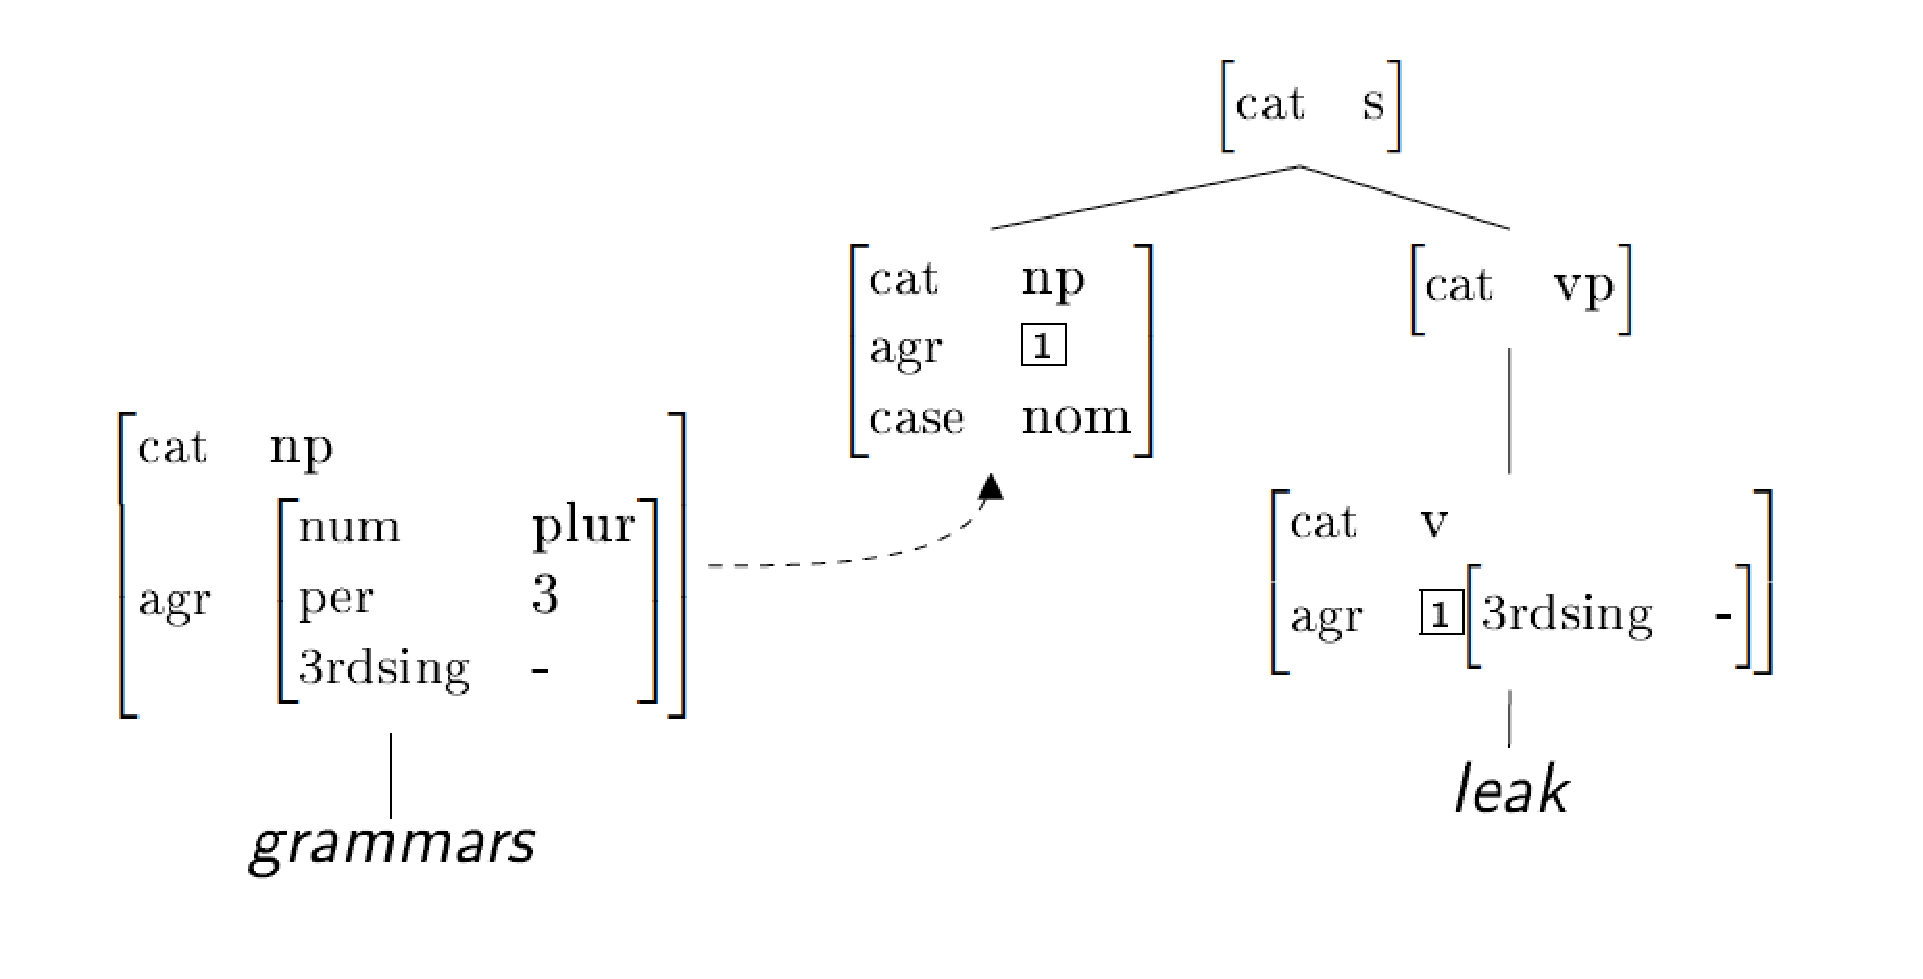
\includegraphics[scale=0.35]{grammarsleak.pdf}
    \caption{Example of a derivation for \textit{``Grammars leak"} with feature structures \label{fig:grleaksubst}}
\end{figure}

However, when adjunction is performed, the adjunction site is practically split in two. In this case, feature structures must be also split. Such a split has been proposed by \citet{Vijay-ShankerJoshi:88}. The idea behind it is that top features should show ``what the node represents in the surrounding structure" and bottom features should show ``what the tree below the node represents".

As a result, in an FTAG all the nodes have a top feature structure and, furthermore, all nodes except substitution nodes have a bottom feature structure. Feature unification applies during the derivation process when adjunction and substitution take place and is performed according to the following rules:
\begin{itemize}
\item when substitution takes place, the top of the root of the rewriting tree unifies with the top of the substitution node;
\item when adjunction takes place, the top of the root of the rewriting tree unifies with the top of the adjunction site, and the bottom of the foot of the rewriting tree unifies with the bottom of the adjunction site (as illustrated by \figref{fig:isleaking} and \figref{fig:isleakingresult}).
\end{itemize}

\begin{figure}
	\centering
    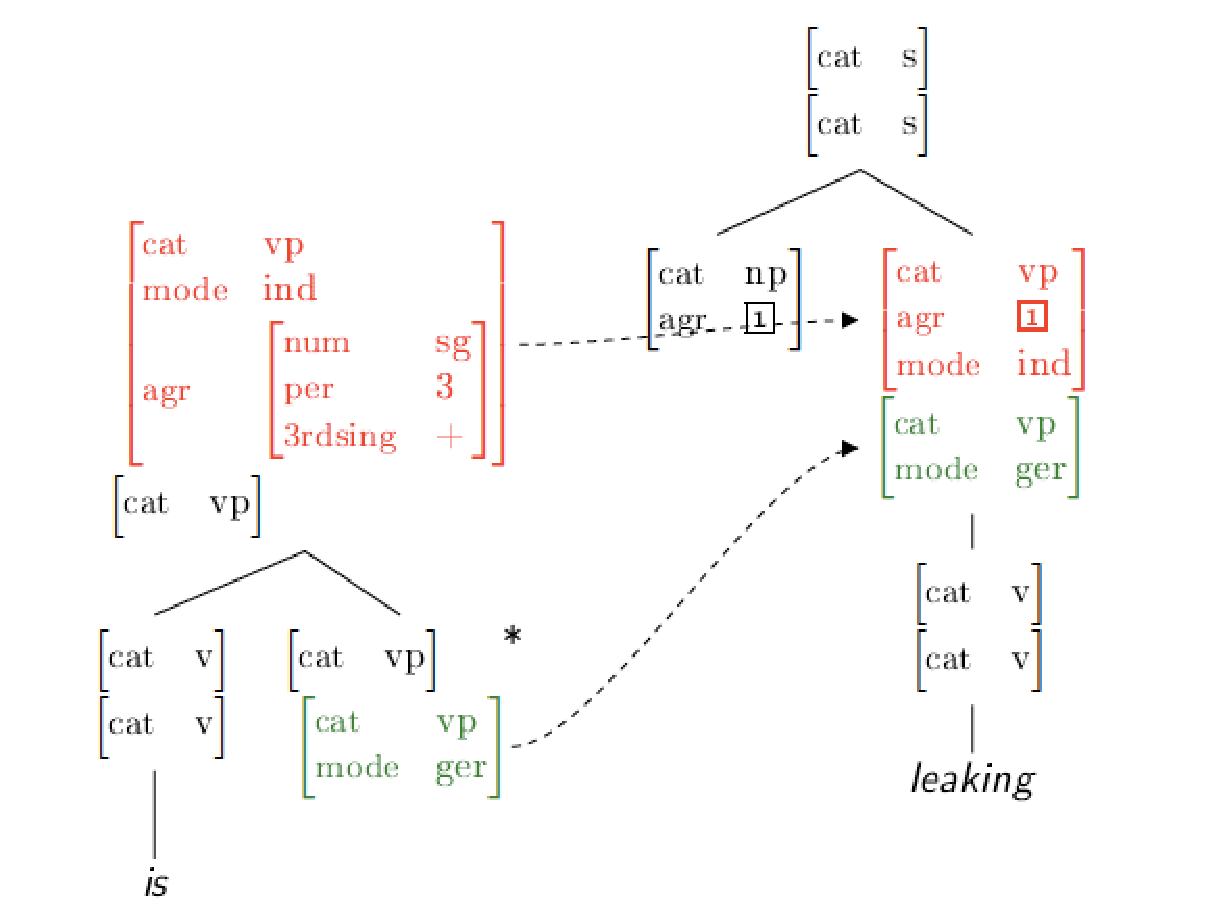
\includegraphics[scale=0.5]{isleaking.pdf}
    \caption{Adjunction of \textit{is} into the tree for \textit{leaking}     \label{fig:isleaking}}
\end{figure}

\begin{figure}
	\centering
    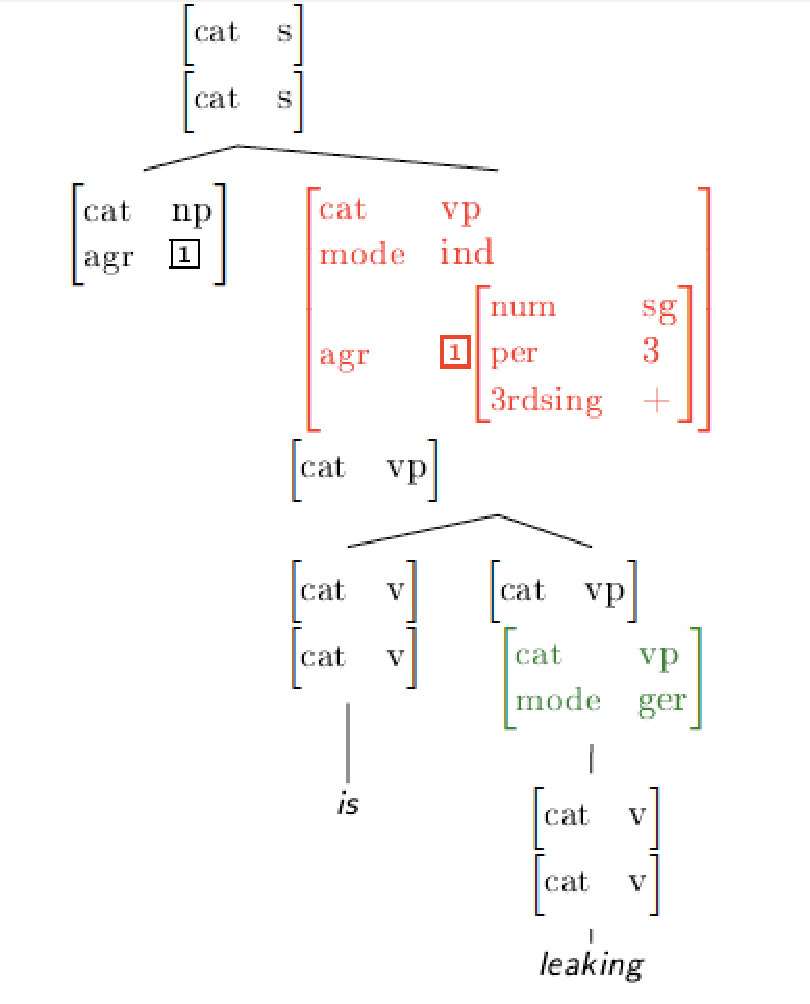
\includegraphics[scale=0.5]{isleakingresult.pdf}
    \caption{Adjunction of \textit{is} into the tree for \textit{leaking}: result \label{fig:isleakingresult}}
\end{figure}

In the final derived tree, top and bottom feature structures unify for all nodes. Feature structures used in an FTAG are allowed to have re-entrancies, but the same attribute should not occur on the path more than once. Due to the extended domain of locality of TAGs, nodes within one elementary tree can share features, allowing to express constraints among dependent nodes easily. On the other hand, the feature structures of FTAG belong to a finite set and thus do not add expressive power, so FTAG and TAG are weakly equivalent.

%To sum up, FTAG is used instead of the simple TAG because feature structures as nodes allow to abstract away from agreement properties by underspecification, which leads to the fact that linguistic generalizations can be expressed more conveniently. Moreover, a split into top and down features provide a convenient mechanism for encoding adjunction constraints, as was illustrated by \figref{fig:isleaking} and \ref{fig:isleakingresult}. Another important fact is that

\paragraph*{Lexicalized TAG} \citet{Abeille:02} and \cite{Frank:02} formulate principles that specify how TAG elementary trees should look like if they are used to model natural languages. First, each elementary tree must have at least one non-empty lexical item. This item is called \textit{lexical anchor}. When all the elementary trees satisfy this condition, a TAG is called \textit{lexicalized TAG,} or LTAG. This property has been argued to be a reasonable requirement with respect to modelling of natural languages. On the computational side it reduces the parsing time. 

The second important principle for a natural language TAG is called \textit{theta-criterion for TAG} \citep{Frank:92}, or \textit{elementary tree minimality}. It requires that every elementary tree with a predicate as a lexical anchor must contain slots (substitution nodes or foot nodes) for all arguments of this predicate (including the subject) and for nothing else. Nominal arguments are usually represented as substitution nodes, whereas sentential arguments are often realised by foot nodes in order to allow long-distance dependency constructions through adjunction  \citep{Kroch:89, Frank:02}.

%\ex.\label{ex:extraction} Whom does John think that Mary hates?

As I have already mentioned, there are several levels of factorization of the LTAG lexicon. The first step is the separation of lexical anchors and tree templates (unanchored elementary trees). As a second step, the set of elementary trees is organized into tree families. Each tree family represents all possible realisations of one subcategorization frame: e.g., there is a tree family for transitive verbs (this means transitive verbs should be used as lexical anchors, i.e. fill the node marked with a diamond). This tree family contains patterns as shown on \figref{fig:treefamily}: canonical position, argument extraction, realization in combination with a passive verb form, among others.

\begin{figure}
\begin{tabular}{l l l}
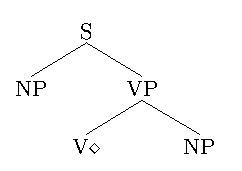
\includegraphics[scale=0.9]{TransVerb.pdf}
&
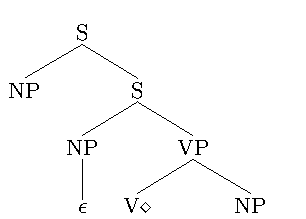
\includegraphics[scale=0.9]{TransVerb2.pdf}
&
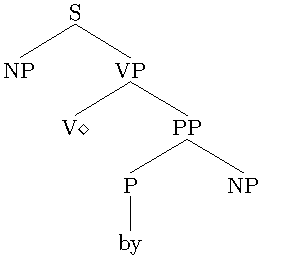
\includegraphics[scale=0.9]{TransVerb3.pdf}
\end{tabular}
\caption{Some elemantary trees from the transitive verb tree family\label{fig:treefamily}}
\end{figure}

The next factorization level is the decomposition of tree templates into tree fragments, that is done using a \textit{metagrammar} description \citep{Candito:99, CrabbeDuchier:04, Crabbe:13}. The idea of the metagrammar is to define tree fragments that can be used in different tree templates and tree families. These tree fragments are minimal models of a constraint system that operates in terms of category assignments and dominance and precedence relations. Such system allows for a compact linguistic description that captures generalizations. 

The level of the metagrammar is well-suited for capturing derivational morphology processes: it allows for a general description of derivational patterns that can be accompanied by a change of the argument structure. I will talk about the technical details of the metagrammar description in Chapter~\ref{Chapter8}. As for now, it is important to know that frames shown in what follows belong to four different description levels: 
\begin{enumerate}
\item frames for the prefixes, frames used for coercion, and dimension constructors accompany special tree fragments that are described in the metagrammar; 
\item frames for the verbs are stored in the dictionary; 
\item frames that represent the result of combining the frame for the derivational base and the prefix frame are obtained when the unanchored trees produced by the metagrammar description get anchored; 
\item frames that represent the semantics of a verbal phrase are obtained on parallel with the syntactic parsing.
\end{enumerate}

\subsection{Frame Semantics}
The idea of using frame representations in linguistic semantics and cognitive
psychology has been put forward by \citet{Fillmore:82} and
\citet{Barsalou:92}, among others. A widescale realisation of this idea is the Berkeley FrameNet project \citep{Fillmore:03}. The goal of this project is to describe a huge variety of situations by basic role frames that represent the type of the situation and the semantic roles of its participants. One issue that FrameNet does not address is modelling compositional semantics: the frames used in the project are static and do not interact with each other. In order to widen the area where frames could be used, a number of studies that offer further formalization of the frame theory has been conducted in the last years \citep[][among others]{Petersen:07, PetersenOsswald:10, KallmeyerOsswald:12, KallmeyerOsswald:13, KallmeyerOsswaldPogodalla:15, Loebner:2014}.

The main ideas that motivate the use of frames as a general semantic and conceptual representation format can be summarized as follows (cf.\ \citealt{Loebner:2014}):
\begin{itemize}
\item conceptual-semantic entities can be described by types and
attributes;
\item attributes are functional relations, i.e., each attribute assigns a unique
value to its carrier;
\item attribute values can be also characterized by types and attributes (recursion);
\item attribute values may be connected by additional relational constraints \citep{Barsalou:92} such as spatial configurations or ordering relations.
\end{itemize}

These ideas are formalized in \citet{KallmeyerOsswald:13} who define frames
as \emph{base-labelled feature structures with types and relations}.
Frames in the sense of \citet{KallmeyerOsswald:13} are finite relational structures in which attributes correspond to functional relations. The members of the underlying set are referred to as the \emph{nodes} of the frame. An important restriction is that any frame must have a \emph{functional
backbone}. This means that every node has to be accessible via attributes
from at least one of the \emph{base nodes}: nodes that carry \emph{base labels}. Importantly, feature structures may have multiple base nodes. In such a case often some nodes that are accessible from different base nodes are connected by a relation.

Base labels serve as unique identifiers, that is, a given base label cannot be assigned to more than one node. Due to the functional backbone requirement, every node of the frame can be addressed by a base label
plus a (possibly empty) finite sequence of attributes.
The middle column of \figref{fig-frame-example} (this figure and \figref{fig-frame-example-II} are provided by Rainer Osswald) illustrates this fact
for the frame depicted on the left of the figure, where circles
represent nodes, the bold-face letters \fsbase{b} and \fsbase{c} are base
labels, labels of solid arrows stand for attributes, labels of dotted arrow
indicated (binary) relations, and the symbols $s$ and $t$ are types.
%
\begin{figure}
\hfill
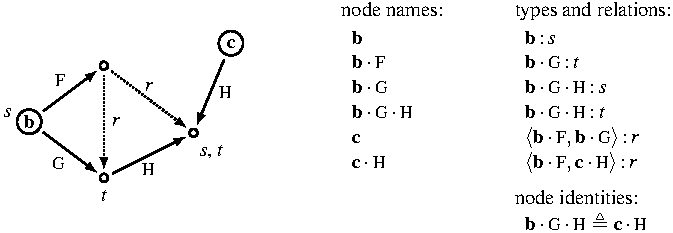
\includegraphics[scale=1.2]{fig-frame-example}
\hfill
\caption{Example of a base-labelled feature structure with types and relations}
\label{fig-frame-example}
\end{figure}%
%

As the example on \figref{fig-frame-example} reveals, a node can have more than one type. The special property of the type system used in frame theory as it is presented in \citealt{KallmeyerOsswald:13} is that type conjunction is always possible unless it violates explicitly stated incompatibility constraints. We will return to the discussion of the type hierarchy in Section~\ref{section:types}.

Frames as attribute-value descriptions can be reformulated in terms of first-order predicate logic and thus related to other semantic representation formats, such as Neo-Davidsonian event semantics. In such a reformulation (fully described in \citealt{KallmeyerOsswald:13}, Section~3.3.3), types and base
labels are regarded as one-place predicates, attributes as two-place predicates, and relation symbols as $n$-place predicates with $n>1$.
In addition, attributes are required to be functional and base labels must
not denote more than one node;
that is, the following two axioms are assumed to hold for all
attributes $f$ and base labels $l$:

\ex.\label{ex.fun-axioms}
$\every u\every v\every w(f(u,v)\und f(u,w)\ifthen v=w)$
\qquad and \qquad
$\every u\every v(l(u)\und l(v)\ifthen u=v)$
%\a.\label{ex.funrel-axiom}
%$\every u\every v\every w(f(u,v)\und f(u,w)\ifthen v=w)$
%\b.\label{ex.funbase-axiom}
%$\every u\every v(l(u)\und l(v)\ifthen u=v)$

The frame shown on \figref{fig-frame-example} can be viewed
as a \emph{model} of the formula shown on the upper left of \figref{fig-frame-example-II} (in the sense of predicate logic). This model also satisfies the formulas given in \ref{ex.fun-axioms}. In what follows I will use frames in form of attribute-value matrices, like the frame shown on the right side of \figref{fig-frame-example-II}.
%
\begin{figure}
\hfill
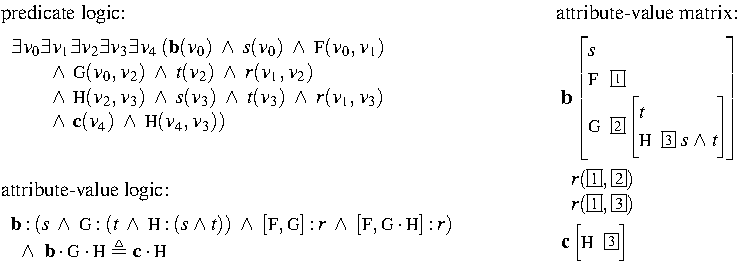
\includegraphics[scale=1.1]{fig-frame-example-II}
\hfill
\caption{Alternative ways of specifying the frame on the left side of
\figref{fig-frame-example}}
\label{fig-frame-example-II}
\end{figure}%
%

For the purposes of a metagrammar specification we need another way of description of frames: attribute-value logic that is defined in \citealt{KallmeyerOsswald:13} (Section~3.3.2). It is constructed as a language of general attribute-value descriptions and then complemented by base labels.

The primitive general attribute-value descriptions over a signature $\langle A, T, R \rangle$ are expressions of the form $t, r, p : t, p \doteq q, p \triangleq q, (p_1, \ldots , p_n) : r$, and $\langle p_1, \ldots , p_n \rangle : r$,
with $p, p_i, q \in A^*, t \in T$, and $r \in R$. For a feature structure $F = \langle V, \delta, \tau, \pi \rangle$ over a signature $\langle A, T, R \rangle$ with $v,w, v_i \in V$ the satisfaction relation $\models$ between attribute-value descriptions and nodes/node tuples of $F$ is defined as shown in \ref{def:satisfaction} (Def.~(3) in \citealt{KallmeyerOsswald:13}).

\ex.\label{def:satisfaction}\a. $v \models t$ ~~~~~~~~~~~~~~~~~~~~~~~~~~~~~~~~~~~~ iff $v \in \tau (t)$
\b. $\langle v_1, \ldots , v_n \rangle \models r$ ~~~~~~~~~~~~~~~~~~~~~~ iff $\langle v_1, \ldots , v_n \rangle \in \rho (t)$
\b. $v \models p : t$ ~~~~~~~~~~~~~~~~~~~~~~~~~~~~~~~~ iff $\delta (v, p) \models t$
\b. $v \models p \doteq q$ ~~~~~~~~~~~~~~~~~~~~~~~~~~~~~~ iff $\delta (v, p) = \delta (v, q)$
\b. $\langle v, w \rangle \models p \triangleq q$ ~~~~~~~~~~~~~~~~~~~~~~~~ iff $\delta (v, p) = \delta (w, q)$
\b. $v \models (p_1, \ldots , p_n ) : r$ ~~~~~~~~~~~~~~~~~~ iff $\langle \delta (v, p_1), \ldots , \delta (v, p_n) \rangle \models r$
\b. $\langle v_1, \ldots , v_n \rangle \models \langle p_1, \ldots , p_n \rangle : r$ ~~~~~ iff $\langle \delta (v, p_1), \ldots , \delta (v, p_n) \rangle \models r$

Labelled attribute-value descriptions are of the form $l \cdot \phi, l \cdot p \triangleq k \cdot q$, and $\langle l_1 \cdot p_1, \ldots , l_n \cdot p_n \rangle : r$, with $k, l, l_i \in B$. The satisfaction conditions are listed in \ref{def:labelled} (Def.~(4) in \citealt{KallmeyerOsswald:13}).

\ex.\label{def:labelled}\a. $\langle F, \beta \rangle \models l \cdot \phi$ ~~~~~~~~~~~~~~~~~~~~~~~~~~~~~~~~~~ iff $\beta (l) \models \phi $
\b.$\langle F, \beta \rangle \models l \cdot p \triangleq k \cdot q $ ~~~~~~~~~~~~~~~~~~~~~~~~~ iff $\langle \beta (l), \beta (k) \rangle \models p \triangleq q$
\b.$\langle F, \beta \rangle \models \langle l_1 \cdot p_1, \ldots l_n \cdot p_n \rangle : r$ ~~~~~~~~~~~~~~~~~~~~~~ iff $\langle \delta (\beta (l_1), p_1), \ldots \delta (\beta (l_n), p_n) \rangle \models r $

Labelled descriptions are allowed to be combined with Boolean operators. The attribute-value matrix shown on the right side of \figref{fig-frame-example-II} can be regarded as a normal form of the attribute-value description given at the bottom of the left side of the same figure. 

\subsection{Combining TAG and Frame Semantics}
There is a number of properties that make LTAG a good candidate for a combination with a frame-based compositional semantics. Two properties are especially important in this respect: the combination of an extended domain of locality and the fact that elementary trees are lexicalized and contain slots for all the arguments of the respective predicate. This allows to link semantic representations directly to the argument slots. It is also convenient that no structural parallelism is required between the syntactic and semantic representations, as argument linking is explicit. The combination of an LTAG and Frame Semantics has been introduced in \cite{KallmeyerOsswald:12} and the most extensive description so far has been provided in \citealt{KallmeyerOsswald:13} (Section~4.1).

In the approach proposed in \cite{KallmeyerOsswald:13} that I adopt here, a single semantic representation (a semantic frame in this case) is linked to the entire elementary tree. When an elementary tree is coupled with a semantic frame, syntactic arguments can be directly linked to their counterpart in the semantics. (Similar approaches with different semantic representation frameworks were introduced earlier in \cite{GardentKallmeyer:03} and \cite{KallmeyerRomero:08}.) Semantic composition is then modelled by unification, which is a result of performing adjunctions and substitutions. \figref{fig:examplesemantic} provides a simple illustration of the syntactic and semantic composition. The feature I on the nodes is a syntax-semantics interface feature. It stands for ``individual'' and is used for argument linking. In this example, substitutions trigger unifications between the nodes \svar{1} and \btag{g} and  between the nodes \svar{2} and \btag{h}. This leads to the correct insertion of the argument frames into the frame of \textit{loves}. The resulting frame representation is shown on Fig.~\ref{frame:love}.
\begin{figure}
	\centering
    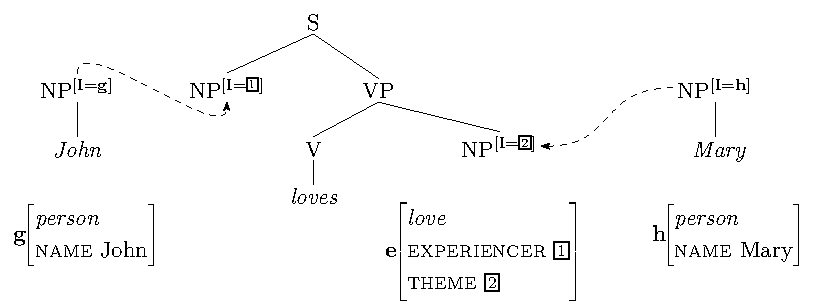
\includegraphics[scale=0.8]{treeJohnLovesMary.pdf} 
    \caption{Syntactic and semantic composition of \textit{John loves Mary}}      
    \label{fig:examplesemantic}
\end{figure}

\begin{figure}
\avm{
\btag{e} [\type*{love}
	   \EXP &  \1 \btag{g} [\type*{person}
	   		\NAME & John ]\\
      \THEME &  \2 \btag{h} [\type*{person}
	   		\NAME & Mary ]
]
}
\caption{Result of frame unifications shown on \figref{fig:examplesemantic} \label{frame:love}}
\end{figure}


\subsection{Type hierarchy}\label{section:types}
The type hierarchy is one of the crucial elements of the analysis, as it is the main mechanism of blocking derivations. Since the number of syntactic restrictions I use is very limited, many derivations will be filtered out by the semantic constraints. For this, there are two main mechanisms: unification failure (type incompatibility or conflicting attribute values) and constraint failure (requirement for the two values to be in a specific relation is not satisfied). 

As I have already mentioned above, any two types can be unified unless there is an explicit constraint that prohibits it. Due to this, adding new types to the type hierarchy is an operation that in most cases can be performed very fast: usually all that one has to do is to specify one or more supertypes of the new type. I will use the term \textit{subtype of type x} to refer to a type that is ordered under the type \textit{x}. Such hierarchy architecture leads to a large number of connections (e.g.\ in comparison with a type hierarchy in HPSG, \citealt{PollardSag:94}), so I will not show the full hierarchy of types used in this chapter, and mostly talk about the relevant restrictive statements (incompatibility of certain types).

The list of types I use for the frames in this chapter and for the implementation to follow can be divided into three major categories (three subtypes of the type \textit{root}): \textit{entity, event,} and \textit{scale.} Among these, \textit{entity} is the only type that is not compatible with the other two. It has subtypes \textit{object} and \textit{person}, that in turn have subtypes and are not compatible with each other. As I do not aim at constructing a large ontology, I use trivial object types and assume that they cannot be unified.

The part of the hierarchy that is more interesting for the current analysis concerns the subtypes of events and scales. Let us start with events. I will be using the following types of events (not compatible with each other): \textit{process, state,} and \textit{transition.} These types can be combined with the event types \textit{bounded-event} and \textit{iteration}. Such classification covers Vendler's \citep{Vendler:67} four-way distinction between states, activities (\textit{process} here), accomplishments (\textit{process $\und$ bounded-event} here), and achievements (\textit{transition}). What is not built into the type system is the distinction between dynamic and static states, that is used, e.g., by \citet{Bach:86}. The rest of the classification proposed in \citealt{Bach:86} is effortlessly expressed: process has the same name, protracted event is a \textit{process $\und$ bounded-event}, happening is \textit{transition}, and culmination is \textit{transition} that has a preparatory phase. These types may have subtypes: e.g., \textit{translocation} and \textit{change-of-state} are subtypes of a process.

The last and most important part of type hierarchy for this work is the domain of scales. The main subtypes of the type \textit{scale} are \textit{closed-scale, one-marked-point, proper-scale, measure-of-change, cardinality}, and \textit{property}. These six types come in three groups such that the subtypes of one group are not compatible with each other. The first group is constituted by the types \textit{closed-scale} and \textit{one-marked-point}, that refer to the presence of end points and are not compatible with each other. To the second group belong the types \textit{measure-of-change} and \textit{proper-scale}. They describe how the scale is organized: in case of a \textit{proper-scale,} for each point of the scale there must be an event stage that is characterized exactly by this point. The \textit{measure-of-change} scale type does not have such requirements: as long as the initial and the final stage of the event are associated with particular scale values, any intermediate stages are allowed. The last group is formed by the \textit{cardinality} and \textit{property-scale} types that refer to the dimension and not to the structure of the scale. Subtypes of the \textit{property-scale} type (such as \textit{color, temperature, length, amount} etc.) are not compatible with each other. The \textit{cardinality} type of the scale allows to talk about iterated events.

A special case is the case of conjunction of the types \textit{event} and \textit{scale}. The idea that underlies it is that events may be conceived as carrying a scalar structure by themselves. One can talk about event \emph{stages} that hold at different moments in the course of the event. Thus, stages are instantaneous situations that are ordered by temporal precedence and can be used to talk about time in connection to the event but without relating this to other events in the world or any kind of a global time representation. For more details, see \citet{ZinovaOsswald:paper}.\footnote{Note that it is not necessary to represent time scales this way, more explicit representations will also be compatible with the frames proposed in this chapter.}
%*Here has to come a picture of the relevant part of the hierarchy*

Now that all the parts needed for the analysis are introduced, let us move to the sections that are dedicated to the particular prefixes.

\section{Frame semantics for the prefix \textit{za-}}\label{section:frame:za}
In this section I propose the frame semantic representation for the inchoative interpretation of the prefix \textit{za-} and show how this prefix combines with a verb. To start, let us recall the conclusions that I have made about the prefix \textit{za-} (in particular about its inchoative interpretation) in Chapter~\ref{Chapter5} by further developing the ideas of \citet{Braginsky:08} and \citet{Kagan:book}. First, I proposed that the inchoative interpretation of the prefix is only possible when the derivational base does not contain any explicit scales except for the time scale in their semantic representation. Second, I offered the following description of the semantic contribution of the prefix \textit{za-} under inchoative interpretation: when the prefix is attached, it relates the initial stage of the event to the state of the absence and the final stage of the event to the state of the presence of the activity denoted by the derivational base.

There are two ways in which the proposed requirement regarding the scale type can be connected with the semantic change caused by the prefix attachment: a `restrictive' one and a `conditional' one. With `restrictive' I mean a straightforward realisation of the proposal above: select only such verbs that have no other scale rather than time (realised with the self-scaling of the event according to the proposal above) in their semantic structure and then describe the semantics of the derived verb in this case. With `conditional' I mean a proposal of such a prefix semantics that, only in case the input verb is related exclusively to the time scale, the desired output (inchoative interpretation of the derived verb) is produced. I pursue the second, more general option. This choice implies the stronger claim that the semantics of the prefix in combination with the semantics of a verb, yields the correct interpretations (probably with some minor modifications or additional constraints) also in cases when the verb is associated with another type of scale (e.g. a \textit{path} scale or a \textit{property} scale). 

\begin{figure}
\centering
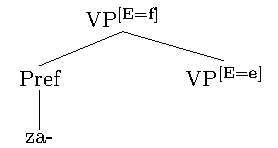
\includegraphics[scale=1]{ZaV.pdf}\\
\begin{tabular}[t]{ll}
\begin{tabular}[t]{l}
\avm{
\btag{f} [\type*{transition}
      \POST & [\type*{event}
         \MDIM & [\type*{proper-scale}
            \MIN & deg ] 
     ]
   ]
}\\
\end{tabular}
\begin{footnotesize}
\begin{tabular}[t]{@{}l@{}}
$\tuple{\btag{f}\BC\POST,\btag{e}}\D\type{esegm-of}$\\[1ex]
$\tuple{\btag{f}\BC\POST\C\MDIM,\btag{e}\BC\MDIM}\D\type{segm-of}$\\
\end{tabular}
\end{footnotesize}
\\\\
\begin{tabular}[t]{l}
\avm{
\btag{e} [\type*{event}
	 \VERBDIM & \1\\
     \MDIM & \1 [\type*{proper-scale}]
   ]
}
\hfill
\end{tabular}
\end{tabular}
\hfill
\caption{Representation of the contribution of the prefix \textit{za-}}
\label{fig.za.frame.semantics}
\end{figure}

The basic frame that I propose in order to represent the general semantic contribution of the prefix \textit{za-} is provided on \figref{fig.za.frame.semantics} together with a tree fragment that represents the attachment of the prefix (and belongs to the metagrammar description). Informally it can be read in the following way: suppose the derivational base denotes some event \textbf{e} that has as its measure dimension some scale of type \textit{proper-scale}. Then the verb prefixed with the prefix \textit{za-} denotes another event that is of type \textit{transition}. A transition is in general characterized by its anterior and posterior states. In this case we are interested in the posterior state that has to be a segment of the event denoted by the derivation base. What we also know is that the scale in the measure dimension of the posterior state of the transition event corresponds to some initial segment of the scale in the measure dimension of the event denoted by the derivational base. The identity of two attributes \VERBDIM and \MDIM of the event frame on Fig.~\ref{fig.za.frame.semantics} ensures that the measure dimension of the event is determined by the verb.

Let me now illustrate what happens when this prefix is attached to a verb. Consider an indeterminate motion verb \textit{begat'} `to run'. The frame representation of this verb is provided on the left side of \figref{frame:begat}. It refers to an event of type \textit{translocation} with the manner of motion of type \textit{run}. The motion leaves some trace and it is performed by some actor. Note that there is no \PATH attribute. This is the assumption made and advocated in \citealt{ZinovaOsswald:paper}, as the \TRACE is regarded to be a set of points the object moved through and thus it is present in the description of any event of type \textit{translocation}. The \PATH attribute is taken to have a more complex structure and be present only in case of a directed motion event.

\begin{figure}
\begin{tabular}[t]{l}
\textit{Verbal base in the dictionary}\\
\avm{
\btag{g} [\type*{transloc}
	   \MANN & [\type*{run}]\relax\\
       \ACTOR & \1\\
	   \TRACE & \2
]
}
\end{tabular}
\hfill
\begin{tabular}[t]{c}
\textit{Verb after dimension constructor}\\
\avm{
\btag{g}  [\type*{transloc $\und$ scale $\und$ time}
	   \MANN & [\type*{run}]\relax\\
       \ACTOR & \1\\
	   \TRACE & \2\\
	   \VERBDIM & \btag{g}  
]
}
\end{tabular}
\caption{Frame representation of an indeterminate motion verb \textit{begat'} `to run' \label{frame:begat}}
\end{figure}

The frame on the right side of \figref{frame:begat} is an enriched variant of the frame on the left: here, information about the verbal dimension is added. Let me explain the idea behind this enrichment in a bit more detail. I claim that from the point of view of the dimension interpretations, all verbs can be divided in two categories: verbs that have a scale they are related to, and verbs that are more flexible in this respect. In the first category fall such verbs as \textit{stoit'} `to cost' (price scale), \textit{gret'} `to warm up' (temperature scale), \textit{mo\v{c}it'} `to make wet' (degree of wetness scale), \textit{letet'} `to fly (directional)' (path scale). 

%For those verbs the measure dimension is already determined in the basic verb representation and cannot be changed. If the direct object is present, it must be able to provide the same measure dimension as is preselected by the verb, usually through the relevant attribute, such as price. Note that such attribute is not necessarily present in the default representation of the object, but can be added, if needed. One can hypothesise that in case the attribute is present by default (e.g., for a house) it would be easier (faster) to use it as a direct object of the verb \textit{stoit'} `to cost' then if such attribute is absent (e.g., for a sky).

The second group of verbs is such that no specific scale is provided in their representation. This means that most of the time these verbs will `accept' the scales `offered' by the direct objects, except for the cases when the prefix demands that the measure dimension is determined by the verb. In these situations the representation of the verb has to be enriched with the information about the scale. The only scale that seems to be generally available as the verbal dimension is the event itself. So the frame on the right side of \figref{frame:begat} obtains an attribute \VERBDIM with a value of type \textit{scale} that has to be identified with the event itself. The type \textit{scale} then gets conjoined with the type \textit{event}. The separation of the dimension information (if this information is not verb-specific) from the rest of the verbal frame (as it is shown by the different states of the frames on the left and right sights of \figref{frame:begat}) allows for a more compact lexicon representation. At the same time it is also possible to store the enriched representation as a dictionary entry and this is in fact what I have to do in the implementation (see Chapter~\ref{Chapter8}) due to the current restrictions of the formalism. 
 
%This procedure is similar for the verbs and the nouns and could be optimized if the formalism would allow to define a set as a value of an attribute and use any member of the set as a measure dimension as long as it satisfies other conditions imposed by the prefix or the context. Such solution is sketched in \citealt{Zinova:14}, but as it cannot be implemented in the current framework, I now offer a less elegant, but implementable variant. 

%To enrich verbal representations with verbal measure dimensions in those cases when this dimension is not fixed, I propose to provide a bunch of constructors that can be applied to the verb and output a minimal VP. First such constructor should only accept those verbs that have a predefined verbal dimension and change nothing. Next option is to use time dimension, that is generally available for any verb (of course when the verbal dimension is already specified, a conflict between the two scales will arise, so there is no need to limit such constructor in any respect). As one can see on the middle frame on \figref{frame:begat}, time scale is not overtly present: it is realised as coreference of the scale and the event itself. 

%Other constructors that are available for a given verb depend on the attributes is has. For example, the verb \textit{begat'} `to run' can acquire verbal dimension of the type \textit{path}, as it has a trace attribute (see the rightmost frame on \figref{frame:begat}). This allows us to explain why in some situations it can be used interchangeably with the directed motion verb \textit{be\v{z}at'} `to run', whereas remaining dispreferred. The preference should be then explained in pragmatic terms, as the determinate motion verb is more specific and thus should be preferred in all the situations where it is suitable to use the path scale.

Now we are ready to unify the verbal frame (on the right side of \figref{frame:begat}) with the prefix frame shown on \figref{fig.za.frame.semantics}. As a result, we obtain the frame for the verb \textit{zabegat'} `to start running' that is presented on \figref{frame:zabegat}. This figure also shows a simplified (no agreement features) initial tree for the derived verb.

\begin{figure}
\centering
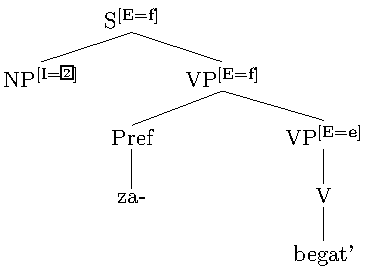
\includegraphics[scale=1]{ZaBegat.pdf}\\
\begin{tabular}[t]{ll}
\begin{tabular}[t]{l}
\avm{
\btag{f} [\type*{transition}
      \POST & [\type*{event}
         \MDIM & [\type*{proper-scale}
         	\MIN & deg ]
     ]
   ]
}\\
\end{tabular}
\begin{footnotesize}
\begin{tabular}{l}
~\\
~\\
$\tuple{\btag{f}\BC\POST,\btag{e}}\D\type{esegm-of}$\\
$\tuple{\btag{f}\BC\POST\C\MDIM,\btag{e}\BC\MDIM}\D\type{segm-of}$\\
\end{tabular}
\end{footnotesize}
\\\\
\begin{tabular}[t]{l}
\avm{
\btag{e} [\type*{event $\und$ transloc $\und$ proper-scale}
      \MDIM & \btag{e}\\
	   \MANN & [\type*{run}]\\
       \ACTOR & \1\\
	   \TRACE & \2\\
	   \VERBDIM & \btag{e}
]
}\\
\end{tabular}
\end{tabular}
\hfill
\caption{Frame representation of the verb \textit{zabegat'} `to start running'}
\label{frame:zabegat}
\end{figure}

The frame on \figref{frame:zabegat} can be read as follows: the verb \textit{zabegat'} `to start running' denotes an event of type \textit{transition} such that the posterior state is a part of a running event and the minimum degree on the event scale after the transition corresponds to the beginning of running. In other words, the combination of the two frames describes a transition from not running into running, which corresponds to the inchoative interpretation. The noun dimension has to agree with the measure dimension, which becomes relevant in case a direct object is present.

Now I would like to spell out two processes: the process of selection of a subpart of the scale that is used as a measure dimension of the new event and the process of obtaining the minimum degree on this scale. The first step is to recall that self-scaling means to consider the event as being itself a scale. From this we can derive a general rule that the minimum of the event scale is always the start of the event and the maximum of the event scale is always the end of the event, so those attribute-value pairs get equated. As a consequence, for this type of the scale the interpretation of the \textit{za-}prefixed verb is inchoative, as the posterior state is associated with the initial portion of the event.

I would like to pay attention to one more detail of the analysis: the type of the scale that is used as a measure dimension. As defined by the prefix frame, this scale has to be a \textit{proper} scale. As I have proposed in Chapter~\ref{Chapter5}, proper scales carry more information than measure of change scales and those two types are incompatible (as stated in the type hierarchy and repeated as a constrain in \ref{const:proper}). With this assumption we can show why sentences as \ref{ex:zabegat:time} are not acceptable, but first we need to construct the frame for the time measure expression \textit{2 \v{c}asa} `for two hours'. 

\ex.\label{const:proper}\textit{proper-scale} $\und$ \textit{measure-of-change} $\rightarrow \bot$

\exg.\label{ex:zabegat:time}\#Vasja zabegal$_{\INDET}$ dva \v{c}asa.\\
Vasya \glb{za}.run.\glb{pst}.\glb{sg}.\glb{m} two hours\\

Let me note that Russian and English time measure expressions are not parallel. For example, the accusative time measure phrase \textit{dva \v{c}asa} `for two hours' can become a part of a prepositional construction \textit{za dva \v{c}asa} `in two hours', which is not possible for English \textit{(*in for two hours)}. Furthermore, it can be used in the \textit{v-}headed prepositional phrase to refer to a point in time (\textit{v dva \v{c}asa} `at two o'clock'). Keeping this in mind, I propose to represent the semantics of the measure expression \textit{dva \v{c}asa} `two hours' as shown on the left side of \figref{frame:2hours}. 

\begin{figure}
\begin{tabular}[t]{c}
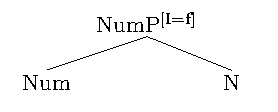
\includegraphics[scale=1]{NumP.pdf}\\
\avm{
\btag{f} [\type*{length}
  		\VAL & 2\\
  		\MUNIT & hour  
  ]
}
\end{tabular}
\hfill
\begin{tabular}[t]{c}
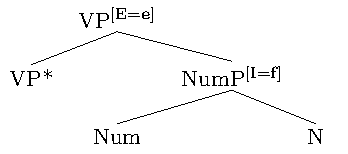
\includegraphics[scale=1]{VNumP.pdf}\\
\avm{
\btag{e}[\type*{event}
  \DURATION & \btag{f}[\type*{length}
  		\VAL & 2\\
  		\MUNIT & hour  
  ]
]
}
\end{tabular}
\caption{Frame representation of the time adverbial \textit{dva \v{c}asa} `for two hours' \label{frame:2hours}}
\end{figure}

Such a representation is neutral with respect to further insertion in various types of constructions and is also shared with other measure-related expressions, such as \textit{p'at' kilometrov} `five kilometres' and \textit{tri kilogramma} `three kilograms'.

In order to combine the measure phrase with a verbal phrase, we need to embed it into the verbal construction as shown on the right side of \figref{frame:2hours}. When this is performed, a VP node becomes the head of the phrase, so the measure expression looses the ability to become a part of a prepositional phrase. At the same time another VP node marked as a footnode is created, so now the measure phrase can be adjoined at a VP node.  On the semantic side a new base node of type \textit{event} is created and the initial representation of the measure phrase becomes the value of the \DURATION attribute of this event.

When the verbal phrase is constructed, constraint \ref{constr:duration} is applied. It states that if the type of the frame is \textit{bounded-event}, than the measure dimension of this event is of type \textit{measure-of-change} and \textit{time}, the minimum on the scale is \textit{zero} and the maximum is equal to the value of the duration.

\ex.\label{constr:duration}\textit{bounded-event} $\und$ (\DURATION = $\top$) $\rightarrow$ (\MDIM = \textit{measure-of-change} $\und$ time) $\und$  \MDIM . \MIN = 0 $\und$ \MDIM . \MAX $\triangleq$ \DURATION .\VAL

%Note that this solution can be improved by creating a system of rules that will assign thematic roles and also determine the slots various measure and path expressions should occupy in the verbal structure. At the moment the asymmetry is explained by the presence of case system that help to determine thematic roles using syntactic information, whereas in the domain of measure expressions only semantic information is left. This problem, however, can be solved, as one can conclude looking at the recent systems of thematic role assignment, such as CITE LAURA?

% the enrichment mechanism is shared with noun phrases in direct object position: for the nouns, their characteristics are stored in the dictionary, but converted to the measure dimension only when they appear in certain constructions. 

\begin{figure}
\hfill
\begin{tabular}[t]{cl}
\txt{za}-V &
\begin{tabular}[t]{l}
\avm{
\btag{f} [\type*{transition}
      \POST & \2 [\type*{event}
         \MDIM & \2 [\type*{proper-scale}
            \MIN & deg ] \\
     ]
   ]
}\\
\end{tabular}
\begin{footnotesize}
\begin{tabular}[t]{l}
$\tuple{\btag{f}\BC\POST,\btag{e}}\D\type{esegm-of}$\\[1ex]
$\tuple{\btag{f}\BC\POST\C\MDIM,\btag{e}\BC\MDIM}\D\type{segm-of}$\\
\end{tabular}
\end{footnotesize}
\\\\
V &
\begin{tabular}[t]{l}
\avm{
\btag{e} [\type*{transloc}
	   \DURATION & [\type*{length}
  			\VAL & 2\\
  			\MUNIT & hour  
   		]\\      
      	\MDIM & \btag{e} [\type*{\color{red}\underline{measure-of-change $\und$ proper-scale $\und$ time}}
			\MIN & 0\\      		
     		\MAX & 2
      	]  \\
	   	\MANN & run\\
       \ACTOR & entity\\
	   \TRACE & trace\\
	   \VERBDIM & \btag{e}
]
}\\
\end{tabular}
\end{tabular}
\hfill
\caption{Failure of unification of the frames for \textit{zabegat'} `to start running' and \textit{dva \v{c}asa}  + `for two hours'}
\label{frame:zabegat:2hours}
\end{figure}

Now we can combine the representation on the right side of \figref{frame:2hours} with the representation of the verb \textit{zabegat'} `to start running' provided on \figref{frame:zabegat}. The unification in this case leads to a conflict due to the type constraint shown in \ref{const:proper}. The combination of the two frames with the underlined conflict is shown on \figref{frame:zabegat:2hours}. 

To complete the picture, let me show that there is no unification failure when the same time measure phrase is combined with a non-prefixed verb. In this case the resulting phrase \textit{begat' dva \v{c}asa} `run for two hours' is perfectly acceptable. Indeed, as the verbal dimension is required to unify with the measure dimension only at the moment of \textit{za-}prefixation, no conflict arises in this case, as the values of the attributes \MDIM and \VERBDIM remain unrelated. The frame can be read as follows: `There is an event of translocation with manner \textit{run} that some actor is involved in. This translocation leaves some trace and has a duration of two hours.' The rest of the frame is not relevant for its final interpretation and, in fact, could be generated at the moment of prefix attachment (this is, however, not possible to implement in the framework I use due to current restrictions of the compiler).

\begin{figure}
\centering
\avm{
\btag{e} [\type*{transloc}
	   \MANN & run\\
       \ACTOR & entity\\
	   \TRACE & trace\\
	   \DURATION & [\type*{length $\und$ time}
  			\VAL & 2\\
  			\MUNIT & hour  
   		]\\ 
	  	\MDIM & [\type*{measure-of-change $\und$ time}
			\MIN & 0\\      		
     		\MAX & 2
   		]\\	   
	   \VERBDIM & \btag{e}
]
}\\
\caption{Frame representation of the verbal phrase \textit{begat' dva \v{c}asa} `run for two hours' \label{frame:begat:2hours}}
\end{figure}

As there is nothing special with the indeterminate motion verbs that could influence the process of combining them with the prefix \textit{za-}, other verbs that have self-reference (\textit{event} $\und$ \textit{scale} type) as the verbal dimension acquire inchoative interpretation in combination with the prefix \textit{za-} in exactly the same way. Let me illustrate this and also the fact that the proposed analysis can be extended to other usages of the prefix \textit{za-} (that occur in presence of other scales) using as an example the verb \textit{\v{z}eltet'} `to be yellow and be seen/to become yellow' that we have discussed in Chapter~\ref{Chapter5}. First let us construct two frames that reflect two interpretations of the basic imperfective verb that probably follow two semantic schemes associated with deriving verbs from color terms. Under the first interpretation, the verb refers to a state of the theme. The color of the theme is (constantly) yellow and the state can be specified as \textit{be seen}. As for any other stative verb, the only available verbal dimension is the event (state) itself. 
\begin{figure}
\begin{tabular}[t]{c}
\textit{to be yellow and be seen}\\
\avm{
 \btag{e} [\type*{state}
  		\STATE & [\type*{be\_seen}]\\
  		\THEME & \1 [
  			\COLOR & [\type*{yellow}]\\
  		]\\
  		\VERBDIM & \btag{e}
  ]
}
\end{tabular}
\hfill
\begin{tabular}[t]{c}
\textit{to become yellow}\\
\avm{
\btag{e} [\type*{change-of-state}
  \VERBDIM & \2 [\type*{property-scale $\und$ yellow} 
  	\MIN & \3\\
  	\MAX & \4  
  ]\\
  \MDIM & \2\\
  \THEME & \1
]
}
\end{tabular}
\caption{Frame representations of the verb \textit{\v{z}eltet'} `to be yellow and be seen/to become yellow' \label{frame:zeltet}}
\end{figure}

The second interpretation is related to a different kind of event -- a change of state. What we know in this situation is that there is a theme that undergoes a change of state along the property scale, more specifically -- a scale of type \textit{yellow}. Note that representing verbal semantics in detail is not the primary focus of this thesis and verbal frames provided here should probably be revised (especially with respect to an accurate representation of change of color), but suffice to show how the prefix \textit{za-} functions.

Let us unify the frame for the prefix \textit{za-} with the frame representations of the verb. We will start with the interpretation of the derivational base that makes use of the event scale (`to be yellow and become seen'). Here everything proceeds exactly as in case of the verb \textit{begat'} `to run' and the frame obtained as a result of the unification describes an event of type \textit{transition} such that the posterior state of this transition corresponds to the initial stage of the event `be yellow and be seen', where `be yellow' is a constant property of the theme, so this means that the derived verb refers to a beginning of the `be seen' state.

\begin{figure}
\begin{tabular}[t]{l}
\textit{za(to be yellow and be seen)}\\
\avm{
\btag{f} [\type*{transition}
      \POST & [\type*{event}
         \MDIM & [\type*{proper-scale}
            \MIN & deg ] \\
     ]
   ]
}\\
\end{tabular}
\begin{footnotesize}
\begin{tabular}[t]{l}
\avm{
\btag{e}[\type*{state $\und$ proper-scale}
  		\STATE & [\type*{be\_seen}]\\
  		\THEME & \2 [
  			\COLOR & [\type*{yellow}]\\
  		]\\
  		\VERBDIM & \btag{e}\\
  		\MDIM & \btag{e}
  ]
}\\
\end{tabular}
\end{footnotesize}
\vspace{0.2em}
\begin{tabular}[t]{l}
$\tuple{\btag{f}\BC\POST,\btag{e}}\D\type{esegm-of}$\\[1ex]
$\tuple{\btag{f}\BC\POST\C\MDIM,\btag{e}\BC\MDIM}\D\type{segm-of}$\\
\end{tabular}
\caption{Frame representation of the verb \textit{za\v{z}eltet'} `to be yellow and become seen' \label{frame:zazeltet:seen}}
\end{figure}

Next I would like to show what happens in the other case: when the verbal dimension is the color property scale. Under this interpretation of the derivational base the transition should have as its posterior state some part of the original event. Which part the posterior state corresponds to is determined by the measure dimension of the derived transition event: the minimum point of the scale has to be included. It is, however, not clear, what the minimum point is, as for the verb \textit{\v{z}eltet'} `to become yellow' it is only given in form of a variable. This means that for the new event (transition) the minimum point on the property scale remains a variable. As a result, we obtain a frame that describes an event of type \textit{transition} with a posterior state corresponding to some yellow state (but we do not know its exact characteristics) of the theme. The underspecification of the scale allows for two interpretations of the derived verb in this case: in the minimum on the scale is some point that can be not considered as being yellow, than the derived verb is interpreted as `to start becoming yellow'; if the minimum on the scale is some point that is yellow, then the derived verb is interpreted as `to become yellow'.

In sum, two representations of the verb combined with one prefix representation yield three possible interpretations of the derived verb: `to be yellow and be seen', `to become yellow', and `to start becoming yellow'. This result agrees with the dictionary data that points exactly to these three meanings of the verb \textit{za\v{z}eltet'}. 

\begin{figure}
\textit{za(to become yellow)}\\
\avm{
\btag{e} [\type*{transition}
      \POST & [\type*{event}
         \MDIM & [\type*{property-scale $\und$ proper-scale $\und$ yellow}
            \MIN & \3
          ] \\
     ]
   ]
}\\
\begin{tabular}[t]{l}
\avm{
\btag{f}[\type*{change-of-state}
  \VERBDIM & \2 [\type*{property-scale $\und$ proper-scale $\und$ yellow} 
  	\MIN & \3\\
  	\MAX & \4  
  ]\\
  \MDIM & \2\\
  \THEME & \1
]
}
\end{tabular}
\hfill
\begin{footnotesize}
\begin{tabular}[t]{l}
$\tuple{\btag{f}\BC\POST,\btag{e}}\D\type{esegm-of}$\\[1ex]
$\tuple{\btag{f}\BC\POST\C\MDIM,\btag{e}\BC\MDIM}\D\type{segm-of}$\\
\end{tabular}
\end{footnotesize}
\caption{Frame representation of the verb \textit{za\v{z}eltet'} `to become yellow/to start becoming yellow' \label{frame:zazeltet:yellow}}
\end{figure}

Another important scale type that can be provided by the verb is \textit{path}. This is the case of determinate motion verbs, such as \textit{be\v{z}at'} `to run (one direction)'. When the frame representation of the prefix \textit{za-} proposed above is combined with the frame representation of such a verb, the resulting interpretation of the derived verb is `transition such that the posterior state is associated with the locomotion that starts at the border of the contextually specified region'. This case is analyzed in detail in \citet{ZinovaOsswald:paper}, so I will skip further details here.

As for the resultative interpretation, some more details and ideas are provided in \citealt{ZinovaKallmeyer:12} and \citealt{Zinova:14}, which address the locative alternation phenomena that in Russian is related to the resultative usage of the prefix \textit{za-}. 

\section{Frame semantics for the prefix \textit{na-}}\label{section:frame:na}
The second prefix that we have discussed in Chapter~\ref{Chapter5} is the prefix \textit{na-} with its cumulative interpretation. As I have concluded after analysing the proposals of \citet{Filip:00} and \citet{Kagan:book} and providing further examples and observations (see discussion in Section~\ref{subsection:semantics:na}), the prefix requires a scale that is provided by the verb and is at the same time a parameter of the object. For example, temperature is a variable parameter for most of the objects, although it may be easier accessible for objects like \textit{soup} than for objects like \textit{book}.


\begin{figure}
\begin{minipage}{0.4\textwidth}
\avm{
\btag{e} [\type*{bounded-event}
	   \NOUNDIM & \3\\       
	   \VERBDIM & \3\\
       \MDIM & \3[\type*{scale}
			\MIN & \1 \\	  
			\THRESHOLD & \2
       ] \\
       \INIT & [\type*{stage}
     		\POS & \1]\\
      \FIN & [\type*{stage} 
  		 	\POS & \4 ]\\
   ]
}\\
\vspace{1cm}
\centering
\svar{2} $\leq$ \svar{4}
\end{minipage}
\hfill
\begin{minipage}{0.4\textwidth}
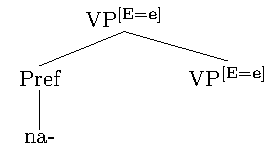
\includegraphics[scale=1]{NaVerb.pdf}\\
\end{minipage}
\caption{Representation of the contribution of the prefix \textit{na-}\label{frame:na}}
\end{figure}

When these requirements are met and the prefix is attached, it maps the minimum point of the scale onto the initial stage of the event and some point that is located at or above the threshold value onto the final stage of the event.  As I have shown earlier, there are cases when a \textit{na-}prefixed verb is compatible with a singular object description. Taking this possibility into account, I propose a frame representation for the prefix as shown on \figref{frame:na}. This frame encodes the following information: the event denoted by a \textit{na-}prefixed verb is a bounded event, the measure dimension is at the same time the verbal dimension and the noun dimension, the initial stage of the event corresponds to the minimum point of the measure dimension scale (that normally is provided by the noun and is identical to the initial value of the relevant property) and the final stage of the event corresponds to the point on the scale that is located at or above the threshold value. 

Note that there is no direct requirement for an open scale, but in many cases it automatically emerges from the semantic restrictions and pragmatic principles alone. The argumentation proceeds in two steps. First, the semantic representation of the event carries a requirement that the event must continue at least until the threshold value on the relevant scale is reached. At the same time the event cannot continue beyond the maximum value on the scale. This means that if there is a maximum value of the property that is supplied by the noun and no information that this maximum value is at least the threshold value, uttering such verb would be pragmatically unsuccessful. Second, suppose the threshold value equals the maximum value on the scale. Then the final stage of the event has to be related to the scale maximum. This is, however, only a special case of the interpretation of a \textit{na-}prefixed verb. If there is another verb that semantically states the equation between the maximum point of the scale and the final stage of the event explicitly, it is preferred over the \textit{na-}prefixed verb for pragmatic reasons (see Chapter~\ref{Chapter6} for more details). 

For example, the verbal phrase \textit{navarila supa} `she made a lot of soup' is interpreted as the quantity of the soup should be significant. This can be explained in terms of a competition with an alternative description \textit{svarila soup} `she made a soup'. If such alternative is absent, then no pragmatic conflict arises in case the maximum of the scale coincides with the threshold: the verbal phrase \textit{naguglit' film} `to google the film' uses the binary scale of the non-found or found state of the object and the maximum on this scale trivially corresponds to the threshold. As there is no other verb that would explicitly equate the maximum value on the scale with the final state, the phrase \textit{naguglit' film} `to google the film' sounds natural. Note, however, that a change of case of the object (\textit{naguglit' filmov} `to google some films') leads to a change of the measure dimension to that of \textit{quantity} that has no inherit maximum and the resulting interpretation is `to find a number of films that is at or above the contextually specified threshold'.

A similar mechanism applies in case another prefixed verb with an excessive interpretation is available. Consider the verb \textit{gret'} `to heat' that has derivatives \textit{peregret'} `to overheat' and \textit{nagret'} `to warm up' that both refer to the same measure dimension: temperature. The \textit{pere-}prefixed verb denotes events the final stage of which is associated with a value strictly above the threshold. In this case the range of events the \textit{na-}prefixed verb denotes gets limited to the events the final stage of which is associated with the threshold value (in our example it is heating the object up to the appropriate temperature). When an alternative \textit{pere-}prefixed verbs is absent (this, for example, is always the case when the measure dimension is of type \textit{quantity}, as in this case the excessive interpretation of the prefix \textit{pere-} is not possible), the \textit{na-}prefixed verb would cover the excessive interpretation domain. 

\begin{figure}
\centering
\avm{
\btag{e} [\type*{change-of-state}
	   \MANN & [\type*{heat}]\\
       \ACTOR & \1\\
	   \THEME & \2\\
	   \VERBDIM & \3 [\type*{temperature}]\\
	   \MDIM & \3
]
}
\caption{Frame representation of the verb \textit{gret'} `to heat' \label{frame:heat}}
\end{figure}

With this in mind let us see how the prefix is combined with some verbs that operate on different scales. We start with the verb \textit{gret'} `to heat' that has as the verbal dimension the temperature scale (that is also copied to the measure dimension attribute). When this verb combines with the prefix \textit{na-}, the resulting frame (provided on \figref{frame:nagret}) denotes a bounded change of state with manner \textit{heat}, some actor, and some theme that has a temperature attribute. The event starts at the temperature corresponding to the minimum of the scale and ends when the temperature is at or above the threshold value. Note that at this moment the minimum on the scale is an unbound variable that will acquire its value later. The threshold value will also be determined only by the pragmatic module that is as well used to block the ``above the threshold'' interpretation of the verb \textit{nagret'} `to warm up', as sketched above.

\begin{figure}
\begin{minipage}{0.50\textwidth}
\avm{
\btag{e} [\type*{bounded-event $\und$ change-of-state}
		\MANN & [\type*{heat}]\\
       \ACTOR & \1\\
	   \THEME & \2\\	   
	   \NOUNDIM & \3\\       
	   \VERBDIM & \3\\
       \MDIM & \3[\type*{scale $\und$ temperature}
			\MIN & \4 \\	  
			\THRESHOLD & \5
       ] \\
       \INIT & [\type*{stage}
     		\POS & \4]\\
      \FIN & [\type*{stage} 
  		 	\POS & \6 ]\\
   ]
}\\
\centering
\svar{5} $\leq$ \svar{6}\\
\end{minipage}
\begin{minipage}{0.45\textwidth}
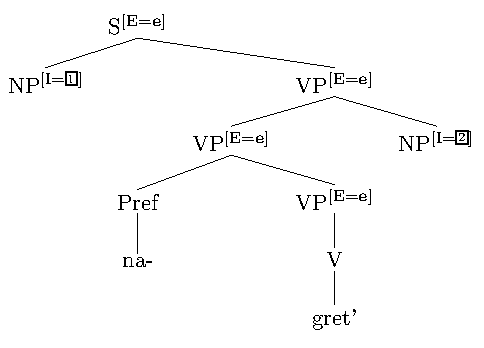
\includegraphics[scale=0.8	]{NaGret.pdf}
\end{minipage}
\caption{Representation of the verb \textit{nagret'} `to warm up' \label{frame:nagret}}
\end{figure}

The next step that is relevant for understanding how prefix frames function is the combination of the verb and the direct object. In our case it is a combination of the verb \textit{nagret'} `to warm up' with some appropriate theme, e.g., \textit{sup} `soup'. Here we would need a similar mechanism of enriching noun representations with dimension information, as I have proposed above for the verbs that do not carry measure dimension information. In our case (see the frame on \figref{frame:soup:dic}) the object of type \textit{soup} has a temperature attribute, as well as an amount attribute, a kind attribute, and a taste attribute. At the same time \textit{amount} and \textit{temperature} can serve as scalar dimensions, which gives rise to the attributes \AMOUNTDIM and \TEMPDIM.  

\begin{figure}
\centering
\avm{
\btag{f} [\type*{soup}
	   \AMOUNT & [\type*{amount}
	   		\VAL & \1\\
	   		\MUNIT & ml ] \\
       \TEMP & [\type*{temperature}
	   		\VAL & \2\\
	   		\MUNIT & degree Celsius ] \\
       \KIND & [\type*{soup-kind}]\\
       \TASTE & [\type*{taste}]\\
       \AMOUNTDIM & [\type*{amount $\und$ measure-of-change}
       		\MIN & 0\\
       		\MAX & \1
       	]\\
       	\TEMPDIM & [\type*{temperature $\und$ proper-scale}
       		\MIN & \2\\ 
       		\MAX & 100
       	]
]
}
\caption{Frame representation of the noun \textit{sup} `soup' \label{frame:soup:dic}}
\end{figure}

Note that the relations between the values of the \AMOUNT and \TEMP attributes of the \textit{soup} and the respective measure dimension specifications differ:  in case of the \textit{amount} dimension, the type of the scale is \textit{measure-of-change} and thus the minimum on the scale is 0. The maximum point of the scale is the value of the \AMOUNT attribute of the \textit{soup}. In case of the \textit{temperature} dimension the value of the \TEMP attribute serves as a minimum point of the respective dimension. The type of the scale is \textit{proper-scale} and the maximum value is 100 (degrees Celsius).

The variability of the minimum or maximum value representation as a static attribute is supported by the variation with respect to which stage is modified by an adjective: if you warm a very cold soup, it is the initial stage of the soup that can be described as \textit{very cold}, but if you write a very long novel, it is the end stage of the novel that can be described as having a length that is greater than the typical length of a long novel. I acknowledge, however, that static representations may prove insufficient: the attribute that provides the relevant dimension undergoes changes and thus is a function of time. However, as such a representation would require significantly more complex modelling and the proposed simplification seems be sufficient for the purposes of current analysis, I will use static representations.

Objects in general may be associated with various measure dimensions, as in case of \textit{soup}, so they have to undergo the process of dimension selection. To perform it, I introduce \textit{dimension constructors} that apply to nouns that have relevant dimensions and identify one of these dimensions with a noun dimension attribute of an event. The first dimension constructor that can be applied to \textit{soup} makes use of the temperature dimension of the noun, identifying it with the value of the attribute \NOUNDIM of the event. The event frame gets linked to a VP that linearly precedes the NP (such constructors are part on the metagrammar description). The semantic and syntactic parts of the constructor are shown on \figref{constructor:temp}. The result of the unification of the temperature dimension constructor frame and the noun phrase frame is shown on \figref{frame:soup:temp}.

\begin{figure}
\begin{minipage}{0.6\textwidth}
\avm{
\btag{e} [\type*{event}
	\THEME & \btag{f} [\type*{entity}
       	\TEMPDIM & \1
	]\\
	\NOUNDIM & \1
]
}
\end{minipage}
\begin{minipage}{0.35\textwidth}
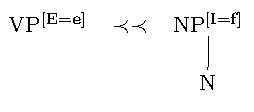
\includegraphics[scale=1]{NaTemp.pdf}
\end{minipage}
\caption{Temperature dimension constructor\label{constructor:temp}}
\end{figure}


\begin{figure}
\centering
\avm{
\btag{e} [\type*{event}
	\THEME & \btag{f} [\type*{soup}
	   \AMOUNT & [\type*{amount}
	   		\VAL & \1\\
	   		\MUNIT & ml ] \\
       \TEMP & [\type*{temperature}
	   		\VAL & \2\\
	   		\MUNIT & degree Celsius ] \\
       \KIND & [\type*{soup-kind}]\\
       \TASTE & [\type*{taste}]\\
       \AMOUNTDIM & [\type*{amount $\und$ measure-of-change}
       		\MIN & 0\\
       		\MAX & \1
       	]\\
       	\TEMPDIM & \3 [\type*{temperature $\und$ proper-scale}
       		\MIN & \2\\ 
       		\MAX & 100
       	]
	]\\
	\NOUNDIM & \3
]
}
\caption{Result of unification of the temperature dimension constructor frame with the frame for the noun \textit{sup} `soup'  \label{frame:soup:temp}}
\end{figure}

The second dimension constructor applicable in case of the noun \textit{sup} `soup' is the amount dimension constructor. It is similar to the temperature dimension constructor shown before, but it also imposes a syntactic requirement for a genitive case of the object. This constructor is shown on \figref{constructor:amount} and the result of the unification of its frame part with the representation of the noun \textit{sup} `soup' is provided on \figref{frame:soup:amount}.

\begin{figure}
\begin{minipage}{0.5\textwidth}
\avm{
\btag{e} [\type*{event}
	\THEME & \btag{f} [\type*{entity}
       \AMOUNTDIM & \1
	]\\
\NOUNDIM & \1
]
}
\end{minipage}
\begin{minipage}{0.35\textwidth}
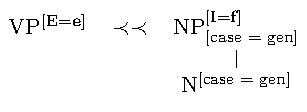
\includegraphics[scale=1]{NPgen.pdf}
\end{minipage}
\caption{Amount dimension constructor \label{constructor:amount}}
\end{figure}

\begin{figure}
\centering
\avm{
\btag{e} [\type*{event}
	\THEME & \btag{f} [\type*{soup}
	   \AMOUNT & [\type*{amount}
	   		\VAL & \1\\
	   		\MUNIT & ml ] \\
       \TEMP & [\type*{temperature}
	   		\VAL & \2\\
	   		\MUNIT & degree Celsius ] \\
       \KIND & [\type*{soup-kind}]\\
       \TASTE & [\type*{taste}]\\
       \AMOUNTDIM & @4 [\type*{amount $\und$ measure-of-change}
       		\MIN & 0\\
       		\MAX & \1
       	]\\
       	\TEMPDIM & [\type*{temperature $\und$ proper-scale}
       		\MIN & \2\\ 
       		\MAX & 100
       	]
	]\\
\NOUNDIM & \4
]
}
\caption{Result of unification of the amount dimension constructor frame with the frame for the noun \textit{sup} `soup' \label{frame:soup:amount}}
\end{figure}

Now we can try combine the representations that emerge from the unification of the noun frame with the  frames of dimension constructors (\figref{constructor:amount} and \figref{constructor:temp}) with the frame for the verb \textit{nagret'} `to warm up' (\figref{frame:nagret}). First let us use the frame that is produced by the temperature dimension constructor (\figref{frame:soup:temp}). The result of inserting the noun representation into the theme slot of the verb in this case is shown on \figref{frame:nagret:soup}. As one can see, now the initial stage of the event corresponds to the initial (minimal) value of the temperature scale associated with the concrete portion of the soup. The final stage is defined as being at least at the threshold value, but not higher than the maximum value. This means that, for example, it would be not possible to heat the soup up to more than 100 degrees Celsius. 

\begin{figure}
\centering
\avm{
\btag{e} [\type*{bounded-event $\und$ change-of-state}
		\MANN & [\type*{heat}]\\
       \ACTOR & \3\\
	   \THEME & \btag{f} [\type*{soup}
	   			\AMOUNT & [\type*{amount}
	   			\VAL & \1\\
	   			\MUNIT & ml ] \\
       		\TEMP & [\type*{temperature}
	   			\VAL & \2\\
	   			\MUNIT & degree Celsius ] \\
       		\KIND & [\type*{soup-kind}]\\
       		\TASTE & [\type*{taste}]\\
       		\AMOUNTDIM & [\type*{amount $\und$ measure-of-change}
       			\MIN & 0\\
       			\MAX & \1
       		]\\
       		\TEMPDIM & [\type*{temperature $\und$ proper-scale}
       			\MIN & \2\\ 
       			\MAX & 100
      	 	]
		]\\
	   \NOUNDIM & \4\\       
	   \VERBDIM & \4\\
       \MDIM & \4 [\type*{temperature $\und$ proper-scale}
				\MIN & \2\\
       			\THRESHOLD & \5
       ] \\
       \INIT & [\type*{stage}
     		\POS & \2]\\
      \FIN & [\type*{stage} 
  		 	\POS & \6 ]\\
   ]
}\\
\textcolor{white}{dd} \svar{5} $\leq$ \svar{6} $\leq$ \textit{100}
\caption{Frame representation of the verbal phrase \textit{nagret' sup} `to warm up the soup' \label{frame:nagret:soup}}
\end{figure}

What if we try to combine the frame for the verb \textit{nagret'} `to warm up' with the same noun \textit{sup} `soup' that went through another dimension constructor? Let us take the representation shown on \figref{frame:soup:amount} and unify it with the frame representation of the verb. When unification is performed, it turns out that the measure dimension of the event has to be simultaneously of types \textit{temperature} and \textit{amount}. This is not possible due to the constraint \ref{const:temp:amount} on type incompatibility. The type conflict that arises in case the amount dimension is selected as the noun dimension is marked on \figref{frame:nagret:soup:amount}. 

\ex.\label{const:temp:amount}\textit{amount} $\und$ \textit{temperature} $\rightarrow \bot$

\begin{figure}
\begin{tabular}{c}
\avm{
\btag{e}  [\type*{bounded-event $\und$ change-of-state}
		\MANN & [\type*{heat}]\\
       \ACTOR & \6\\
	   \THEME & \btag{f} [\type*{soup}
	   		\AMOUNT & [\type*{amount}
	   			\VAL & \1\\
	   			\MUNIT & ml ] \\
       		\TEMP & [\type*{temperature}
	   			\VAL & \2\\
	   			\MUNIT & degree Celsius ] \\
       		\KIND & [\type*{soup-kind}]\\
       		\TASTE & [\type*{taste}]\\
       		\AMOUNTDIM & \5[\type*{amount $\und$ measure-of-change}
       			\MIN & 0\\
       			\MAX & \1
       		]\\
       		\TEMPDIM & [\type*{temperature $\und$ proper-scale}
       			\MIN & \2\\ 
       			\MAX & 100
      	 	]
		]	\\
	   \NOUNDIM & \5\\       
	   \VERBDIM & \5\\
       \MDIM & \5 [\type*{\textcolor{red}{\underline{temperature $\und$ amount $\und$ measure-of-change}}}
				\MIN & 0\\
       			\THRESHOLD & \3
       ] \\
       \INIT & [\type*{stage}
     		\POS & 0]\\
      \FIN & [\type*{stage} 
  		 	\POS & \4 ]\\
   ]
}\\
\svar{3} $\leq$ \svar{4}
\end{tabular}
\caption{Failure during the unification of the frames for \textit{nagret'} `to warm up and  \textit{sup} `soup' with amount dimension interpretation \label{frame:nagret:soup:amount}}
\end{figure}

The mechanism of type conflict is the main mechanism that prevents unwanted prefix stacking and inappropriate measure phrases or direct object interpretations. Note, however, that noun representations allow for different interpretations and the concrete interpretation is only selected relative to an event. This means that the same noun can be viewed as providing different dimensions when several event nodes are present in the semantic structure. This is even possible with one verb (secondary imperfective verb with habitual/iterative interpretation) due to different measure dimensions of the iterated subevent and the event that refers to the whole series of subevents.

Another way of implementing the same system of agreement between the dimensions of the verb and the noun is to formulate requirements (here, for example, a requirement for a temperature scale), but in the current version of the formalization of Frame Semantics within XMG 2 that I am using here it is not possible. For this reason such requirements have to appear implicitly as type or value incompatibilities. I leave it to future research to find out whether an approach that uses constructors and type conflicts is cognitively plausible.

%As type constraints are universal (type hierarchy is only provided once) and type conflict situations are symmetric. E.g., a type of \textit{open scale} could make sense only for the situations when such scale is inherently open, i.e. no end points might be added by any further specifications; this is so because if one uses this type for any open scale, then after the end points are added, the type will become \textit{open scale $\und$ close scale}; if these two types are said to be incompatible, we will loose the ability to add end points. If they are compatible, the specification of an \textit{open scale} type is redundant. This symmetry limits the expressive power of the constraint system and I hope that in the near future linguists and cognitive scientists will find out which system is cognitively more plausible.

Let me provide one more example of the interaction between the prefix \textit{na-}, a verb, and a direct object. This time we will consider the verb \textit{varit'} `to cook' as the base verb. The frame representation of this verb is provided on the left side of \figref{frame:varit} and shows that there is no preselected verbal dimension. At the same time the frame uncovers the parameter of the cooking event: apart from the type of the theme, the quantity (amount) of the cooked food plays a role. I propose to introduce a dimension constructor that
\begin{enumerate}
\item constructs a measure dimension of the type \textit{amount};
\item is only available if the next step is the attachment of the prefix \textit{na-};
\item can be applied if the verbal frame contains a specification of the amount of one of the arguments.
\end{enumerate}

If such constructor is used, the verbal representation acquires the corresponding measure dimension, as shown on the right side of \figref{frame:varit}. In contrast to the noun dimension constructors, no changes on the syntactic side are associated with the verbal dimension constructor. At the same time, as stated above, it can be only used in connection with \textit{na-}prefixation. 

\begin{figure}
\begin{tabular}[t]{l}
\avm{
\btag{e} [\type*{process}
	   \MANN & [\type*{cook}]\\
       \ACTOR & \2\\
	   \THEME & [\type*{food}
	   		\AMOUNT & \1 ]
]
}
\end{tabular}
\hfill
\begin{tabular}[t]{l}
\avm{
\btag{e} [\type*{process}
	   \MANN & [\type*{cook}]\\
       \ACTOR & \2\\
	   \THEME & [\type*{food}
	   		\AMOUNT & \1 ]\\
	   \VERBDIM & [\type*{amount $\und$ measure-of-change}
	   		\MIN & 0\\
	   		\MAX & \1
	   ]
]
}
\end{tabular}
\caption{Frame representation of the verb \textit{varit'} `to cook' before (left) and after (right) an enrichment with scalar information \label{frame:varit}}
\end{figure}

Now the verb has a \VERBDIM argument and can be combined with the prefix frame. The result of the unification of the frame on \figref{frame:na} with the frame on the right side of \figref{frame:varit} is shown on \figref{frame:navarit}. It describes a bounded process that starts with no food being cooked and ends when some amount of food that exceeds the threshold is cooked. The \textit{measure-of-change} type of the \textit{amount} scale ensures that there is no requirement for any intermediate event stage to correspond to some intermediate value on the amount scale, so no gradual cooking in terms of amount is required, which means that the soup may be prepared as one portion.

\begin{figure}
\begin{tabular}{c}
\avm{
\btag{e}[\type*{bounded-event $\und$ process}
		\MANN & [\type{cook}]\\
       \ACTOR & \6\\
	   \THEME & [\type*{food}
	   		\AMOUNT & \1 ]\\
	   \VERBDIM & \2 [\type*{amount $\und$ measure-of-change}
	   		\MIN & 0 \\
	   		\MAX & \1
	   ]\\
	   \NOUNDIM & \2\\   
       \MDIM & \2[\type*{scale}
			\MIN & \3\\	  
			\THRESHOLD & \4\\
       ] \\
       \INIT & [\type*{stage}
     		\POS & 0
      ]\\
      \FIN & [\type*{stage} 
  		 	\POS & \5 
  	]\\
   ]
}\\
\svar{4} $\leq$ \svar{5}\\
\end{tabular}
\caption{Frame representation of the verb \textit{navarit'} `to cook a lot of' \label{frame:navarit}}
\end{figure}

As a next step, we try to combine the representation of the verb \textit{navarit'} `to cook a lot of' with two possible interpretations of the noun \textit{sup} `soup' that we have discussed above (see \figref{frame:soup:temp} and \figref{frame:soup:amount}). Here the result is opposite to that with the verb \textit{nagret'} `to warm up': the temperature-related interpretation of the noun fails to serve as the theme of the event, while the amount interpretation can be successfully used. The unification failure in the first case is due to the type conflict that is marked on \figref{frame:navarit:soup:temp}. The type compatibility constraints are violated two times: \textit{amount} conflicts with \textit{temperature} (see \ref{const:temp:amount}) and \textit{proper-scale} conflicts with \textit{measure-of-change} (see \ref{const:proper}).

\begin{figure}
\begin{tabular}{c}
\avm{
 \btag{e} [\type*{bounded-event $\und$ process}
		\MANN & [\type*{cook}]\\
       \ACTOR & \1\\
	   \THEME & [\type*{soup}
	   		\AMOUNT & [\type*{amount}
	   			\VAL & \4\\
	   			\MUNIT & ml ] \\
       		\TEMP & \btag{f}[\type*{temperature}
	   			\VAL & 0\\
	   			\MUNIT & degree Celsius ] \\
       		\KIND & [\type*{soup-kind}]\\
       		\TASTE & [\type*{taste}]\\
       		\AMOUNTDIM & [\type*{amount $\und$ measure-of-change}
       			\MIN & 0\\
       			\MAX & \1
       		]\\
       		\TEMPDIM & \3
		]	\\
	   \NOUNDIM & \3\\       
	   \VERBDIM & \3\\
       \MDIM & \3 [\type*{\textcolor{red}{\underline{amount $\und$ temperature  $\und$ measure-of-change $\und$ proper-scale}}}
				\MIN & 0\\
				\MAX & 100\\       
       			\THRESHOLD & \5
       ] \\
       \INIT & [\type*{stage}
     		\POS & 0 ]\\
      \FIN & [\type*{stage} 
  		 	\POS & \6 ]\\
   ]
}\\
\svar{5} $\leq$ \svar{6} $\leq$ \textit{100}
\end{tabular}
\caption{Failure of unification of the frame for the verb \textit{navarit'} `to cook a lot of' and the frame for the noun \textit{sup} `soup' with temperature dimension interpretation \label{frame:navarit:soup:temp}}
\end{figure}

Note that this representation format stores a lot of world knowledge: not only the resulting verbal frame in case of the verb \textit{nagret'} `to warm up' contains information that the event of warming something proceeds along the temperature scale, but the frame for the verb \textit{navarit'} `to cook' also carries the knowledge that it is not the temperature domain that is relevant in this case, although temperature changes are definitely present during the cooking process. At the same time selection of the amount dimension of the verb is a special case and the proposed architecture does not prevent the event from being measured in other terms (e.g., degree of being cooked) when the verb is prefixed with other prefixes.

Now, when we combine the appropriate amount-related representation of the noun \textit{sup} `soup' (in genitive case) with the frame for the verb \textit{navarit'} `to cook a lot of', unification is successfully performed. The resulting frame for the verbal phrase \textit{navarit' supa} `to cook a lot of soup', shown on \figref{frame:navarit:soup:amount}, can be read as follows: a bounded process of cooking is performed by some actor. The theme of the event is \textit{soup} that was not present (zero amount value) at the initial stage, but is present at the final stage of the event. The amount of soup cooked at the end of the event equals or exceeds the threshold value. 

\begin{figure}
\begin{tabular}{c}
\avm{
\btag{e} [\type*{bounded-event $\und$ process}
		\MANN & [\type*{cook}]\\
       \ACTOR & \2\\
	   \THEME & \btag{f} [\type*{soup}
	   		\AMOUNT & [\type*{amount}
	   			\VAL & \1\\
	   			\MUNIT & ml ] \\
       		\TEMP & [\type*{temperature}
	   			\VAL & 0\\
	   			\MUNIT & degree Celsius ] \\
       		\KIND & [\type*{soup-kind}]\\
       		\TASTE & [\type*{taste}]\\
       		\AMOUNTDIM & \3 \\
       		\TEMPDIM & [\type*{temperature $\und$ proper-scale}
       			\MIN & 0\\ 
       			\MAX & 100
      	 	]
		]	\\
	   \NOUNDIM & \3\\       
	   \VERBDIM & \3\\
       \MDIM & \3 [\type*{amount  $\und$ measure-of-change}
				\MIN & 0\\
       			\THRESHOLD & \4\\
       			\MAX & \1
       ] \\
       \INIT & [\type*{stage}
     		\POS & 0 ]\\
      \FIN & [\type*{stage} 
  		 	\POS & \5 ]\\
   ]
}\\
\svar{4} $\leq$ \svar{5} $\leq$ \svar{1}
\end{tabular}
\caption{Frame representation of the verbal phrase \textit{navarit' supa} `to cook a lot of soup' (amount dimension interpretation of the noun) \label{frame:navarit:soup:amount}}
\end{figure}


\section{Frame semantics for the prefix \textit{po-}}\label{section:frame:po}
The next prefix I provide a frame representation of is \textit{po-}. In Chapter~\ref{Chapter5} on the basis of the analyses proposed by \citet{Filip:00} and \citealt{Kagan:book} and an extensive data discussion, I have concluded that all the usages of the prefix \textit{po-} can be unified under one underspecified semantic representation. As has already been observed by \citet{Kagan:book}, the prefix \textit{po-} can be attached to different types of scales. In the default case, the scale is one of the verbal scales. In addition, if the event denoted by the derivational base is of type \textit{iteration}, a \textit{cardinality} scale can be provided by the direct object and used as an event scale. As shown on the left side of \figref{frame:po:delim}, the prefix adds information that the event is bounded and the initial and the final stages of the event are related to arbitrary points on the scale.

\begin{figure}
\begin{minipage}{0.4\textwidth}
\avm{
\btag{e} [\type*{bounded-event}
   	   \VERBDIM & \1\\
       \MDIM & \1 [\type*{scale}] \\
       \INIT & [\type*{stage}
     		\POS & \2]\\
       \FIN & [\type*{stage} 
  		 	\POS & \3 ]\\
   ]
}
\end{minipage}
\begin{minipage}{0.55\textwidth}
\avm{
 \btag{e} [\type*{bounded-event $\und$ transloc $\und$ scale}
   		\MANN & [\type*{run}]\\
   		\ACTOR & \1\\
   		\TRACE & [\type*{trace}]\\
   	   \VERBDIM &  \btag{e}\\
       \MDIM & \btag{e}\\
       \INIT & [\type*{stage}
     		\POS & \2]\\
       \FIN & [\type*{stage} 
  		 	\POS & \3 ]\\
   ]
}
\end{minipage}
%% Add requirement that if m-dim = path, path-start = init
\caption{Frame representations of the prefix \textit{po-} (left) and of the verb \textit{pobegat} `to run for some time' (right) \label{frame:po:delim}}
\end{figure}

Although the prefix does not provide information about the exact scalar degrees associated with the initial and final stages of the event, in some cases the derived verb carries such information. This happens when the measure dimension is the event itself and thus the \MIN and \MAX attributes of the scale become promoted to the event level. In this case the initial and the final stages need to be identified with the maximum and the minimum points on the scale. This is done via constraints shown under \ref{rule:minmaxevent}.

\ex.\label{rule:minmaxevent}\a. \MIN = $\top$ $\und$ \INIT = $\top$ $\rightarrow$ \INIT.\POS $\triangleq$ \MIN
\b. \MAX = $\top$ $\und$ \FIN = $\top$ $\rightarrow$ \FIN.\POS $\triangleq$ \MAX

Let us now combine the frame representation of the prefix \textit{po-} with the verbal frames that we have already considered above. The first verb is an indeterminate motion verb \textit{begat'} `to run'. The only dimension constructor the prefix \textit{po-} has access to (in case the verb has no specified measure dimension) is the self-scaling constructor. This means that the prefix frame can be combined with the frame on the right side of \figref{frame:begat}. The result of the unification of the enriched verbal frame with the prefix frame (\figref{frame:po:delim}) is provided on the right side of \figref{frame:po:delim}. The derived frame can be interpreted as describing a bounded event of translocation with manner \textit{run}, some actor and some trace, that started at some point and ended at some other point. To ensure that the two degrees on the scale differ from each other, I assume a general constraint shown in \ref{const:diff}.

\ex.\label{const:diff}\textit{bounded-event} $\rightarrow$ \INIT.{\POS} $\neq$ \FIN.\POS

If now this verb is combined with a temporal measure phrase, such as \textit{dva \v{c}asa} `two hours' (see the frame on the right side of \figref{frame:2hours}), the verbal phrase \textit{pobegat' dva \v{c}asa} `to run for two hours' receives the frame representation shown on \figref{frame:pobegat:2hours}. Two things has to be taken into account at this point due to the fact that the measure dimension is the event itself. First, all the information about the measure dimension needs to be ``passed'' to the event level. Afterwards, constraints \ref{constr:duration} and \ref{rule:minmaxevent} are applied. As a result, (1) the event representation acquires the complex type \textit{bounded-event $\und$ transloc $\und$ scale $\und$ measure-of-change $\und$ time}, (2) the minimum of the measure dimension is equated with the minimum of the event and with the scale degree that corresponds to the initial stage of the event, and (3) the maximum of the measure dimension is equated with the maximum of the event and with the scale degree that corresponds to the final stage of the event.

\begin{figure}
\centering
\avm{
   \btag{e}[\type*{bounded-event $\und$ transloc $\und$ measure-of-change $\und$ time}
   		\MANN & [\type*{run}]\\
   		\ACTOR & [\type*{entity}]\\
   		\TRACE & [\type*{trace}]\\
   		\DUR & [\type*{length $\und$ time}
			\VAL & 2\\
			\MUNIT & hour   		
   		]\\
   	   \VERBDIM &  \btag{e}\\
       \MDIM &  \btag{e}\\
       \INIT & [\type*{stage}
     		\POS & 0]\\
       \FIN & [\type*{stage} 
  		 	\POS & 2]\\
  		\MIN & 0\\
  		\MAX & 2
   ]
}\\
%% Add requirement that if m-dim = path, path-start = init
\caption{Frame semantics of the verbal phrase \textit{pobegat dva \v{c}asa} `to run for two hours' \label{frame:pobegat:2hours}}
\end{figure}


In order to see how the representation of the prefix \textit{po-} interacts with other verbal scales, let us consider the verb \textit{gret'} `to heat' that denotes a change along the temperature dimension (\figref{frame:heat}). The derived verb \textit{pogret'} `to warm up' refers to a bounded change of state of the theme. This change happens along the temperature dimension, but no particular values are associated with the initial and the final stages of the event. The resulting frame can be interpreted as `there is an event of manner \textit{heat} that lead to some increase of the temperature'.

\begin{figure}
\centering
\avm{
 \btag{e} [\type*{bounded-event $\und$ change-of-state}
   		\MANN & [\type*{heat}]\\
   		\ACTOR & [\type*{entity}]\\
   		\THEME & [\type*{entity}]\\
   	   \VERBDIM & \1 [\type*{temperature}]\\
       \MDIM & \1\\
       \INIT & [\type*{stage}
     		\POS & \2 ]\\
       \FIN & [\type*{stage} 
  		 	\POS & \3 ]
   ]
}\\
%% Add requirement that if m-dim = path, path-start = init
\caption{Frame semantics of the verb \textit{pogret'} `to warm up' \label{frame:pogret}}
\end{figure}

Now let us proceed to the case when the prefix \textit{po-} is interpreted distributively. This occurs when an argument of the verb supplies a cardinality scale that is used to measure the event. For this situation to be available, the initial event has to be of type \textit{iteration} or has to be compatible with such interpretation.\footnote{In the latter case the distributive interpretation usually has to be supported by an overt quantifier.} The only special tool that we need to account for this case is the constraint \ref{const:card} that introduces \textit{iteration} type in case something of type \textit{event} is simultaneously of type \textit{cardinality}. 

\ex.\label{const:card}\textit{event $\und$ cardinality $\rightarrow$ iteration}

%This frame refers to a bounded iteration event that is measured using the cardinality scale without strict internal structure (this means that several objects may be affected at the same time). The event starts when 0 members of the set the cardinality of which is used as a measure dimension are affected and ends when all the members of that set are affected. 
%\begin{figure}
%\centering
%\avm{
%\btag{e}  [\type*{bounded-event}
%   \NOUNDIM & \3\\
%    \MDIM & \3 \[
%       \type*{cardinality}
%       \MIN & \1\\
%       \MAX & \2]\\
%    \INIT & [\type*{stage}
%       \POS & \1 ]\\
%     \FIN & [\type*{stage}
%       \POS & \2 ]
%  ]
%}
%\caption{Semantic representation of a \textit{po-}prefixed verb \label{frame:po:distr}}
%\end{figure}
 
 \begin{figure}
% \begin{minipage}{0.45\textwidth}
\hfill\avm{
\btag{e} [\type*{event $\und$iteration}
    \MANN & [\type*{burst}]\\
    \ACTOR & \1\\
    \THEME & \2\\
    \VERBDIM & \btag{e}
  ]
}
% \end{minipage}
% \begin{minipage}{0.5\textwidth}
\hfill%
\avm{
\btag{e} [\type*{iteration $\und$ bounded-event $\und$ scale}
    \MANN & [\type*{burst}]\\
    \ACTOR & \1\\
    \THEME & \2\\
    \VERBDIM & \btag{e}\\
    \MDIM & \btag{e} \\
    \INIT & [\type*{stage}
     		\POS & \3]\\
    \FIN & [\type*{stage} 
  		 	\POS & \4 ]\\
  ]
}\hfill%
% \end{minipage}
\caption{Frame representations of the verbs \textit{lopat'} `to burst' (left) and \textit{polopat'} `to burst for some time/all of' (right) \label{frame:lopat}}
\end{figure}
 
Let us consider the case where a non-quantified object can cause the distributive interpretation of the verb. To do this, we will look at the semantics of the verb \textit{lopat'} `to burst' and its derivatives. As an event of bursting is punctual, the default interpretation of the imperfective verb is iterative, so the type of the frame on \figref{frame:lopat} is \textit{iteration}. The verbal dimension is the event itself. When this verb is prefixed with \textit{po-}, the result of the unification is the frame shown on the right side of \figref{frame:lopat}.

\begin{figure}
\small
% \begin{minipage}{0.575\textwidth}
\avm{
\btag{e} [\type*{event}
	\THEME & \btag{f} [\type*{entity}
       \CARD & [\type*{cardinality}
       		\POS & \1
       	]
	]\\
\MDIM & [\type*{cardinality}
			\MIN & 0\\
       		\MAX & \1
       	]
]
}
% \end{minipage}
\hfill%
\begin{minipage}[c]{0.4\textwidth}
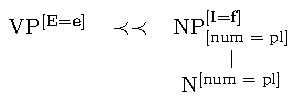
\includegraphics[scale=1]{NPpl.pdf}
\end{minipage}
\caption{Cardinality dimension constructor\label{constructor:cardinality}}
\end{figure}

The second ``ingredient'' for the verbal phrase \textit{polopat' \v{s}ary} `to burst the balloons' is the noun \textit{\v{s}ar} `balloon' that has to supply some measure dimension, which in this case is the cardinality scale. The constructor of the cardinality scale, shown on \figref{constructor:cardinality}, is similar to the constructors introduced before. What differs on the syntactic side is the presence of the requirement for the plural number of the noun. As for the semantic side, here the information about the scale of the event is passed directly into the \MDIM attribute and not into the \NOUNDIM attribute. Informally speaking, this means that once the cardinality constructor applies, the cardinality scale must be used. At the same time the usage of this constructor needs to be restricted to cases when the noun is a direct object of a verb that denotes an event of type \textit{iteration}. 

The frame representation of the noun \textit{\v{s}ar} `balloon' is shown on the right side of \figref{frame:balloon}. The right side of the same figure shows the result of unification of the noun representation with the cardinality dimension constructor.

\begin{figure}\small
% \begin{minipage}{0.4\textwidth}
\avm{
\btag{f} [\type*{balloon}
	   \CARD & [\type*{cardinality}
       		\POS & \1
       	]\\
       \SIZE & \2\\
       \COLOR & \3
]
}
% \end{minipage}
\hfill%
% \begin{minipage}{0.575\textwidth}
\avm{
\btag{e} [\type*{event $\und$ iteration}
	\THEME & \btag{f} [\type*{balloon}
	   \CARD & [\type*{cardinality}
       		\POS & \1
       	]\\
       \SIZE & \2\\
       \COLOR & \3]\\
    \MDIM & [ \type*{cardinality}
        \MIN & 0\\
       	\MAX & \1 ]
]
}
% \end{minipage}
\caption{Frame representations of the noun  \textit{\v{s}ar} `balloon' (left) and of the result of its unification with the cardinality dimension constructor (right) \label{frame:balloon}}
\end{figure}

Now we are ready to combine the verbal and the nominal frames and obtain the representation of the verbal phrase \textit{polopat' \v{s}ary} `to burst the balloons' that is shown on \figref{frame:burst:balloon}. The frame describes a bounded iteration event of bursting. The actor is not yet specified, and the theme is of type \textit{balloon} with some cardinality, size, and color. The event is measured along the cardinality dimension: it starts when zero balloons are burst and ends when all the balloons are burst. There is no information about the internal structure of the bursting event, apart from the \textit{iteration} type. This means that several balloons could be burst at once as long as there are multiple bursting sub-events.

\begin{figure}
\centering
\avm{
\btag{e} [\type*{bounded-event $\und$ iteration $\und$ cardinality}
    \MANN & [\type*{burst}]\\
    \ACTOR & \5\\
    \THEME & [\type*{balloon}
	   \CARD & [\type*{cardinality}
       		\POS & \1
       	]\\
       \SIZE & \2\\
       \COLOR & \3\\
    ]\\
    \VERBDIM & \btag{e}\\
    \MDIM & \btag{e}\\
    \MIN & 0\\
    \MAX & \1\\
    \INIT & [\type*{stage}
       \POS & 0 ]\\
     \FIN & [\type*{stage}
       \POS & \1 ]
  ]
}\\
\hfill
\caption{Frame representation of the verbal phrase \textit{polopat' \v{s}ary} `to burst the balloons' \label{frame:burst:balloon}}
\end{figure}

Note that the interpretation of the same phrase that describes the bursting event only in terms of time is also possible. As the prefix frame in case of \textit{po-} only requires the verbal dimension to be present, the application of the dimension constructor is not obligatory. This means that we can unify directly the frame for the verb \textit{polopat'} `to burst for some time/all of' on the right side of \figref{frame:lopat} and the frame for the noun \textit{\v{s}ar} `balloon' provided on the left side of \figref{frame:balloon}. The result of this unification is shown on \figref{frame:burst:delim}. Such an interpretation of the verbal phrase \textit{polopat' \v{s}ary} `to burst balloons' is indeed possible and can be paraphrased as `to spend some time bursting balloons'. 

\begin{figure}
\centering
\avm{
\btag{e} [\type*{bounded-event $\und$ iteration $\und$ scale}
    \MANN & [\type*{burst}]\\
    \ACTOR & \6\\
    \THEME & [\type*{balloon}
	   \CARD & \1\\
       \SIZE & \2\\
       \COLOR & \3
    ]\\
    \VERBDIM & \btag{e}\\
    \MDIM & \btag{e}\\
    \INIT & [\type*{stage}
       \POS & \4 ]\\
     \FIN & [\type*{stage}
       \POS & \5 ]
  ]
}\\
\hfill
\caption{Frame representation of the verbal phrase \textit{polopat' \v{s}ary} `to burst balloons for some time' \label{frame:burst:delim}}
\end{figure}

\section{Frame semantics for the prefix \textit{pere-}}\label{section:frame:pere}
The next prefix, \textit{pere-}, is the most polysemous of Russian verbal prefixes. As I have argued in Section~\ref{subsection:semantics:do}, starting with the proposals of \citet{Demjjanow:97} and \citet{Kagan:book} and providing further data and observations, several representations are required to acquire different interpretations of the prefix, although the process of selection is fully dependent on the type of the scale.

The first representation accounts for spatial (crossing), time-related (passing the time, waiting), and distributive usages. It applies when the measure dimension is such scale that there is a possibility to map each degree on the scale onto the event stages. In particular, this requires the scale to be closed. The second representation applies when there is only one marked point on the relevant scale (e.g., excessive and `outdo' usages). In this case the event proceeds from some point below the marked point through the marked point point to the point above it. The last representation leads to the iterative interpretation of the event. In this case the derived verb refers to a new event that has as its preparatory phase the event denoted by the derivational base. I will now show these representations one by one. 

\subsection{Distributive, crossing and waiting interpretations}
The first frame representation is, on the one hand, the most `ordinary', as it resembles a lot the frames we have already discussed. On the other hand, it covers three ``traditional'' usages. As we have already discussed a number of similar frames, I will now only point out what is special in this case (the frame is shown on \figref{frame:pere:distr}). As before, the key restrictive factor is the type of the measure dimension: a closed proper scale in this case. The source of this scale is the noun, if it is not already specified by the verb (in this case the noun has to offer an appropriate scale). The initial and final stages of the event correspond to the minimum and maximum points on the scale. 
\begin{figure}
\centering
\avm{
\btag{e}  [\type*{bounded-event}
   \NOUNDIM & \3\\
    \MDIM & \3 [
       \type*{closed-scale $\und$ proper-scale}
       \MIN & \1\\
       \MAX & \2]\\
    \INIT & [\type*{stage}
       \POS & \1 ]\\
     \FIN & [\type*{stage}
       \POS & \2 ]
  ]
}
\caption{Frame representation of the prefix \textit{pere-}: case of a closed scale \label{frame:pere:distr}}
\end{figure}

Let me now illustrate how this prefix frame combines with the representations of the verbs. First consider the verb \textit{zimovat'} `to spend winter time' that we have discussed in Chapter~\ref{Chapter6}. This verb has as the verbal dimension the time scale, as many verbs, but this scale is predefined already in the lexicon, so no choice of dimension constructors is possible. The frame for this verb is shown on \figref{frame:zimovat}. (The choice of the type of the manner and the representation of the extremes of the scale may be revised.) Note that the fact that the verbal frame contains information about the minimum and the maximum of the scale does not lead to a bounded interpretation of the verb: it arises only in presence of the \INIT and \FIN attributes.

\begin{figure}
\centering
\avm{
  \btag{e} [\type*{process $\und$ closed-scale}
    \MANN & [\type*{spend-time $\und$ winter}]\\
    \ACTOR & \1\\
    \VERBDIM & \btag{e}\\
    \MDIM & \btag{e}\\
    \MIN &  [\type*{winter-start}]\\
    \MAX &  [\type*{winter-end}]\\
  ]
}\\
\hfill
\caption{Frame representation of the verb \textit{zimovat'} `to spend winter time' \label{frame:zimovat}}
\end{figure}

Now we can combine the frame for the verb \textit{zimovat'} `to spend winter time' with the frame for the prefix \textit{pere-}. The result of the unification of the two frames is shown on \figref{frame:perezimovat}. This new frame refers to a bounded process of spending winter time that starts when the winter starts and ends when the winter ends. In other words, it is an event of spending the whole winter, which corresponds to the meaning of the verb. The identity of the scale minimum with the initial stage of the event and of the scale maximum with the final stage of the event is established due to the constraints shown in \ref{rule:minmaxevent}.

\begin{figure}
\centering
\avm{
\btag{e} [\type*{process $\und$ bounded-event $\und$ closed-scale $\und$ proper-scale}
    \MANN & [\type*{spend-time $\und$ winter}]\\
    \ACTOR & \3\\
    \VERBDIM & \btag{e}\\
    \NOUNDIM & \btag{e}\\
    \MDIM & \btag{e}\\
    \MIN &  \1 [\type*{winter-start}]\\
    \MAX &  \2 [\type*{winter-end}]\\
     \INIT & [\type*{stage}
       \POS & \1 ]\\
     \FIN & [\type*{stage}
       \POS & \2 ]
  ]
}
\caption{Frame representation of the verb \textit{perezimovat'} `to spend the winter' \label{frame:perezimovat}}
\end{figure}

The second example is the case of the path scale. Consider a determinate motion verb \textit{be\v{z}at'} `to run'. The frame representation of this verb (on the left side of \figref{frame:bezhat}) differs from the frame representation of the indeterminate motion verb \textit{begat'} `to run' (shown on \figref{frame:begat}) in that it contains a \PATH attribute and the \textit{path} scale is selected as a measure dimension. 

\begin{figure}
\begin{minipage}{0.4\textwidth}
\avm{
\btag{e} [\type*{transloc}
	   \MANN & [\type*{run}]\\
       \ACTOR & \1\\
	   \TRACE & [\type*{trace}]\\
	   \PATH & \2 [\type*{path}]\\
	   \VERBDIM & \2\\
	   \MDIM & \2
]
}
\end{minipage}
\begin{minipage}{0.55\textwidth}
\avm{
\btag{e} [\type*{bounded-event $\und$ transloc}
	   	\MANN & [ \type*{run} ]\\
       	\ACTOR & \4\\
	   \PATH & \1\\
	   	\TRACE & [ \type*{trace} ]\\
	   	\VERBDIM & \1 \\
	   	\MDIM & \1 [ \type*{path $\und$ closed-scale $\und$ proper-scale}
       		\MIN & \2\\
       		\MAX & \3
       	]\\
      	\NOUNDIM & \1\\
    	\INIT & [\type*{stage}
       		\POS & \2 ]\\
     	\FIN & [\type*{stage}
       		\POS & \3 ]
  ]
}
\end{minipage}
\caption{Frame representations of the determinate motion verb \textit{be\v{z}at'} `to run' (left) and of the verb \textit{perebe\v{z}at'} `to run accross' (right) \label{frame:bezhat}}
\end{figure}

When the verb \textit{be\v{z}at'} `to run' combines with the prefix \textit{pere-}, the frame for the derived verb refers to a bounded translocation event of manner \textit{run} that is measured according to the \textit{path} that has to be also the measure dimension of the noun. The event starts at the minimum point of the path and ends at the maximum point of the path. This frame is shown on the right side of \figref{frame:bezhat}.

What is still missing in this frame is the specification of the path that has to come from the noun. This has to be a closed path across the object the noun refers to. I propose to use a dimension constructor that takes as its input any object that has width or diameter (or, probably, some other attribute) and outputs a path across this object. This path is probably still underspecified, as information from the context is needed to find out at least on which ``side'' of the landmark the movement starts. So if we start with a dictionary noun representation, such as shown on the left side of \figref{frame:road}, it can be unified with the constructor shown on \figref{constructor:path}. This constructor is similar to those we have already seen. It specifies the \NOUNDIM attribute of the event as being of type \textit{path}. This path is located in the \LOC of the landmark. The extreme points of this path belong to the set of the edge points of the landmark. There should be an extra condition that ensures that the path goes to the ``opposite'' side, but this is hard (if possible) to formalize (at least in the purely semantic terms and especially for such objects that do not have distinct edges, e.g., a lake), so I will leave this problem for future research.  

\begin{figure}\small
\begin{minipage}{0.3\textwidth}
\avm{
\btag{e} [ \type*{event}
	\PATH & \1 [ \type*{path}
		\MIN & \2\\
		\MAX & \3
	]
]
}\end{minipage}\hfill%
\begin{minipage}{0.3\textwidth}\centering
\avm{
\btag{f} [\type*{landmark}
       	\EDGE & \4 \\
       	\LOC & \5 ]
}\\
\svar{1} $\in$ \svar{5} $\und$ \svar{2} $\in$ \svar{4} $\und$ \svar{3} $\in$ \svar{4}
\end{minipage}\hfill%
\begin{minipage}{0.25\textwidth}
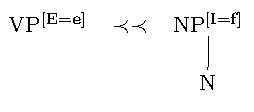
\includegraphics[scale=.8]{NaTemp.pdf}
\end{minipage}
\caption{Path dimension constructor\label{constructor:path}}
\end{figure}

\begin{figure}\small
% \begin{minipage}{0.35\textwidth}
\avm{
\btag{f} [\type*{road}
	   \WIDTH & \1\\
	   \LOC & \2\\
	   \EDGE & \3
]
}\hfill%
% \end{minipage}
% \begin{minipage}{0.25\textwidth}
\avm{
\btag{e} [\type*{event}
	\PATH & \6[\type*{path}
		\MIN & \4\\
		\MAX & \5
	]
]
}\hfill%
% \end{minipage}
\begin{minipage}{0.275\textwidth}
\avm{
\btag{f} [\type*{landmark $\und$ road}
	   \WIDTH & \1\\
	    \LOC & \2\\
       	\EDGE & \3 ]
}\\
\vspace{0.3em}
\svar{4} $\in$ \svar{3} $\und$ \svar{5} $\in$ \svar{3} $\und$ \svar{6} $\in$ \svar{2}
\end{minipage}
\caption{Frame representations of the noun \textit{doroga} `road' (left) and of its unification with the path dimension constructor (right) \label{frame:road}}
\end{figure}

Now we are ready to combine the verbal frame that is shown on the right side of \figref{frame:bezhat} with the noun representation that is unified with the dimension constructor (shown on the right side of \figref{frame:road}. The result of the unification is provided on \figref{frame:cross:road}. In the derived frame the noun contributes information about the path across the landmark that becomes the measure dimension of the event.

\begin{figure}
\small
\begin{minipage}{0.6\textwidth}
\avm{
\btag{e} [\type*{bounded-event $\und$ transloc}
	   	\MANN & [ \type*{run} ]\\
       	\ACTOR & \4\\
	    \PATH & \1\\
	   	\TRACE & [ \type*{trace} ]\\
	   	\VERBDIM & \1 \\
	   	\MDIM & \1 [ \type*{path $\und$ closed-scale} \type*{$\und$ proper-scale}
       		\MIN & \2\\
       		\MAX & \3
       	]\\
      	\NOUNDIM & \1\\
    	\INIT & [\type*{stage}
       		\POS & \2 ]\\
     	\FIN & [\type*{stage}
       		\POS & \3 ]
  ]
 }
\end{minipage}\hfill%
\begin{minipage}{0.35\textwidth}
\avm{
 \btag{f} [\type*{landmark $\und$ road}
	   \WIDTH & \5\\
	    \LOC & \6\\
       	\EDGE & \7]
}\\
\vspace{0.3em}
\svar{1} $\in$ \svar{6} $\und$ \svar{2} $\in$ \svar{7} $\und$ \svar{3} $\in$ \svar{7}
\end{minipage}
\caption{Frame representation of the verbal phrase \textit{perebe\v{z}at' dorogu} `to run accross the road' \label{frame:cross:road}}
\end{figure}


To illustrate how the distributive interpretation of the verb is obtained with the same prefix frame, let us take the verb \textit{lopat'} `to burst' and the noun \textit{\v{s}ar} `balloon' that we have already used to illustrate the distributive usage of the prefix \textit{po-}. The resulting frame representation of the phrase \textit{perelopat' \v{s}ary} `to burst all the balloons' is shown on \figref{frame:pereburst:balloon} and differs from the frame for the phrase \textit{polopat' \v{s}ary} `to burst the balloons' shown on \figref{frame:burst:balloon} only with respect to the type of the scale that represents the measure dimension. Now the type is not \textit{measure-of-change,} but \textit{proper-scale}. This means that the scale description now contains not only the extreme points, but also all the natural numbers between zero and the cardinality of the set of balloons. So the iteration of the bursting sub-events now has to proceed from zero burst balloons to one burst balloon, to two burst balloons, etc. No simultaneous bursting of two or more balloons is allowed. The \textit{proper-scale} type is a compact way to encode this difference between two distributive interpretations.

\begin{figure}
\centering
\avm{
\btag{e} [\type*{bounded-event $\und$ iteration}
    \MANN & [\type*{burst}]\\
    \ACTOR & \5\\
    \THEME & [\type*{balloon}
	   \CARD & \1\\
       \SIZE & \2\\
       \COLOR & \3\\
       \NOUNDIM & \4\\
    ]\\
    \VERBDIM & \btag{e}\\
    \NOUNDIM & \4\\
    \MDIM & \4 [ \type*{cardinality $\und$ proper-scale $\und$ closed-scale}
       		\MIN & 0\\
       		\MAX & \1
     ]\\
    \INIT & [\type*{stage}
       \POS & 0 ]\\
     \FIN & [\type*{stage}
       \POS & \1 ]
  ]
}\\
\hfill
\caption{Frame representation of the verbal phrase \textit{perelopat' \v{s}ary} `to burst all the balloons' \label{frame:pereburst:balloon}}
\end{figure}

\subsection{Excessive interpretation}
The next sub-meaning of the prefix \textit{pere-} that we are going to discuss occurs if the scale has only one marked point. In this case the initial stage of the event is associated with some point of the scale that lays below the marked point and the end stage of the event is associated with some point of the scale that lays above the marked point. Often this point would be the same as the threshold value that we have used for the prefix \textit{na-}. Similarly to the case of the distributive/crossing usage of the prefix \textit{pere-} that we have considered above, the measure dimension should correspond to the dimension provided by the noun. The frame that encodes these ideas is provided on \figref{frame:pere:over}.
\begin{figure}
\begin{center}
\begin{tabular}{c}
\avm{
\btag{e} [\type*{bounded-event}
  	\NOUNDIM & \4\\
    \MDIM & \4 [
       \type*{proper-scale $\und$ one-marked-point}
       \MARKED & \2 ]\\
    \INIT & [\type*{stage}
       \POS & \1 ]\\
     \FIN & [\type*{stage}
       \POS & \3 ]\\
  ]
}\\
\svar{1} $<$ \svar{2} $<$ \svar{3}
\end{tabular}
\end{center}
\caption{Frame representation of the prefix \textit{pere-}: case of a scale with one marked point \label{frame:pere:over}}
\end{figure}

Let us see what happens if this prefix usage is combined with the verb \textit{gret'} `to heat' and the noun \textit{sup} `soup' that we have discussed above. The frame on \figref{frame:pere:gret} represents the semantics of the verb \textit{peregret'} `to overheat' obtained by the unification of the frame on \figref{frame:pere:over} with the frame on \figref{frame:heat}. It refers to a bounded change of state with manner \textit{heat} that starts with the temperature of the theme being below the marked point and ends with the temperature of the theme being above the marked point.

\begin{figure}
\begin{center}
\begin{tabular}{c}
\avm{
 \btag{e} [\type*{bounded-event $\und$ change-of-state}
  	\MANN & [ \type*{heat}]\\
  	\ACTOR & \5\\
  	\THEME & \6\\
  	\NOUNDIM & \4\\
  	\VERBDIM & \4\\
    \MDIM & \4 [
       \type*{proper-scale $\und$ one-marked-point $\und$ temperature}
       \MARKED & \2 ]\\
    \INIT & [\type*{stage}
       \POS & \1 ]\\
     \FIN & [\type*{stage}
       \POS & \3 ]\\
  ]
}\\
\svar{1} $<$ \svar{2} $<$ \svar{3}
\end{tabular}
\end{center}
\caption{Frame representation of the verb \textit{peregret'} `to overheat' \label{frame:pere:gret}}
\end{figure}

Next we combine the frame for the verb \textit{peregret'} `to overheat' with the frame for the noun \textit{sup} `soup' that has been unified with the temperature dimension constructor. As a result, as expected, we obtain the frame that describes an event of heating of the soup that starts from the temperature lower than the marked temperature (marked temperature in this case is the same as the threshold value in case of the \textit{na-}prefixed verb) and ends when the temperature is greater than the marked temperature.

\begin{figure}
\begin{center}
\begin{tabular}{c}
\avm{
 \btag{e} [\type*{bounded-event $\und$ change-of-state}
  	\MANN & [ \type*{heat}]\\
  	\ACTOR & \6\\
  	\THEME & [\type*{soup}
	   \AMOUNT & [\type*{amount}
	   		\VAL & \1\\
	   		\MUNIT & ml ] \\
       \TEMP & [\type*{temperature}
	   		\VAL & \2\\
	   		\MUNIT & degree Celsius ] \\
       \KIND & [\type*{soup-kind}]\\
       \TASTE & [\type*{taste}]\\
       \AMOUNTDIM & [\type*{amount $\und$ measure-of-change}
       		\MIN & 0\\
       		\MAX & \1
       	]\\
       	\TEMPDIM &  \4[\type*{temperature $\und$ proper-scale}
       		\MIN & \2\\ 
       		\MAX & 100
       	]
	]\\
  	\NOUNDIM & \4\\
  	\VERBDIM & \4\\
    \MDIM & \4 [
       \type*{proper-scale $\und$ one-marked-point $\und$ temperature}
       \MARKED & \2 \\
    ]\\
    \INIT & [\type*{stage}
       \POS & \5 ]\\
     \FIN & [\type*{stage}
       \POS & \3 ]\\
  ]
}\\
\svar{5} $<$ \svar{2} $<$ \svar{3}
\end{tabular}
\end{center}
\caption{Frame representation of the verbal phrase \textit{peregret' sup} `to overheat the soup' \label{frame:pere:gret:soup}}
\end{figure}

The next class of derivational bases to which the same frame for the prefix \textit{pere-} can be attached is constituted by directed motion verbs such as \textit{letet'} `to fly'. The frame for the base verb, shown on \figref{frame:letet} is similar to that of the verb \textit{be\v{z}at'} `to run' (\figref{frame:bezhat}).\footnote{The verb \textit{be\v{z}at'} `to run' cannot be used in combination with the discussed interpretation of the prefix \textit{pere-}. I cannot tell the exact reason for this, but it seems to be related to the granularity. The `over' meaning of the prefix \textit{pere-} arises with all semelfactive motion verbs, such as \textit{prygnut'} `to jump once' and with some but not all activity-denoting motion verbs. The latter class probably can be described as those verbs that refer to a manner of motion that cannot be denoted by a semelfactive verb. My analysis does not explain the difference between the verbs \textit{be\v{z}at'} `to run' and \textit{letet'} `to fly' in this respect and I hypothesize that this difference lays outside of the semantic domain. } The only difference is the value of the \MANN attribute.

\begin{figure}
\centering
\avm{
\btag{e} [\type*{transloc}
	   \MANN & [\type*{fly}]\\
       \ACTOR & \1\\
	   \TRACE & [\type*{trace}]\\
	   \PATH & \2 [\type*{path}]\\
	   \VERBDIM & \2\\
	   \MDIM & \2
]
}
\caption{Frame representation of the determinate motion verb \textit{letet'} `to fly' \label{frame:letet}}
\end{figure}

When the frame for the verb \textit{letet'} `to fly' is unified with the frame representation of the prefix \textit{pere-} (\figref{frame:pere:over}), we obtain the frame shown on \figref{frame:pere:letet}. This frame describes a bounded translocation event of manner \textit{fly} that starts at some point of the path below the marked point and ends at some point of the path that is above the marked point. The marked point has to be provided by the noun, as the nominal dimension is equated to the measure dimension of the whole event. 

\begin{figure}
\begin{center}
\begin{tabular}{c}
\avm{
 \btag{e} [\type*{bounded-event $\und$ transloc}
  	\MANN & [\type*{fly}]\\
	\ACTOR & \tag{0}\\  	
  	\VERBDIM & \4\\
  	\NOUNDIM & \4\\
  	\PATH & [\type*{path}]\\
  	\TRACE & [\type*{trace}]\\
    \MDIM & \4 [
       \type*{proper-scale $\und$ one-marked-point $ \und$ path}
       \MARKED & \2 ]\\
    \INIT & [\type*{stage}
       \POS & \1 ]\\
     \FIN & [\type*{stage}
       \POS & \3 ]\\
  ]
}\\
\svar{1} $<$ \svar{2} $<$ \svar{3}
\end{tabular}
\end{center}
\caption{Frame representation of the verb \textit{pereletet'} `to fly over' \label{frame:pere:letet}}
\end{figure}

For this to be possible, the object has to be conceptualized as having an almost zero width (or the width smaller than one unit of motion, e.g., one step). The marked point is then the coordinate of the crossing place that can be obtained by intersecting the motion vector with the representation of the object. It is probable that only the projections on the two dimensional space (surface of the group) are considered while finding this point and constructing the relevant path. I will not describe the mechanism of finding this point and just assume that it exists and provides the relevant point based on the information about the location of the object. As shown on \figref{frame:road:point}, the constructor that generates this type of the measure dimension also sets the value of the \WIDTH attribute to \textit{epsilon} and uses a constraint that the marked point has to belong to the set of points provided as a value of the \LOC attribute.

\begin{figure}
\begin{minipage}{0.31\textwidth}
\avm{
\btag{f} [\type*{road}
	   \WIDTH & [\type*{epsilon}]\\
	   \LOC & \2\\
	   \EDGE & \1 ]
}
\end{minipage}\hfill%
\begin{minipage}{0.6\textwidth}\centering
\avm{
\btag{e} [\type*{event}
	   \NOUNDIM & [ \type*{path $\und$ one-marked-point}
			\MARKED & \3]
]
}\\
\svar{3} $\in$ \svar{2}
\end{minipage}
\caption{Frame representation of the noun \textit{doroga} `road' unified with the constructor of one point path \label{frame:road:point}}
\end{figure}

If the representation of the verb \textit{pereletet'} `to fly over', shown on \figref{frame:pere:letet}, is combined with the representation of the noun \textit{doroga} `road' that provides information about a one point scale, we obtain the frame shown on \figref{frame:pere:letet:road}. Note that the representation of the accusative noun does not become a value of any attribute and stays connected only through the relation of inclusion of the marked point into the path. Such representation of a relation between a path-related landmark and the motion along the path is also used in the analysis of English motion expressions proposed in \citealt{KallmeyerOsswald:13}, e.g., for the sentence \textit{John walked along the brook} \citep[Fig.~23, p. 32]{KallmeyerOsswald:13}.

\begin{figure}
\begin{minipage}{0.66\textwidth}
\avm{
\btag{e} [\type*{bounded-event $\und$ transloc}
  	\MANN & [\type*{fly}]\\
	\ACTOR & \tag{0}\\  	
  	\VERBDIM & \4\\
  	\NOUNDIM & \4\\
  	\PATH & \4\\
  	\TRACE & [\type*{trace}]\\
    \MDIM & \4 [
       \type*{proper-scale $\und$} \type*{one-marked-point $ \und$ path}
       \MARKED & \2 ]\\
    \INIT & [\type*{stage}
       \POS & \1 ]\\
     \FIN & [\type*{stage}
       \POS & \3 ]\\
  ]
}
\end{minipage}%
\begin{minipage}{0.33\textwidth}\centering
\avm{
\btag{f} [\type*{road}
	   \WIDTH & [\type*{epsilon}]\\
	   \LOC & \6\\
	   \EDGE & \5
]
}\\
\svar{2} $\in$ \svar{6}\\\svar{1} $<$ \svar{2} $<$ \svar{3}
\end{minipage}
\caption{Frame representation of the verbal phrase \textit{pereletet' dorogu} `to fly over the road' \label{frame:pere:letet:road}}
\end{figure}

As in this case the measure dimension of the event is the noun dimension, the same noun enriched with the crossing interpretation (as shown on the right of \figref{frame:road}) cannot be combined with the verb \textit{pereletat'} `to fly over' as shown on the \figref{frame:pere:letet}. The conflict that arises in this case is due to the constraint \ref{const:one:closed} and is marked on \figref{frame:pere:letet:road:red}.

\ex.\label{const:one:closed}\textit{one-point-scale} $\und$ \textit{closed-scale} $\rightarrow \bot$

\begin{figure}
\begin{minipage}{0.7\textwidth}
\avm{
\btag{e} [\type*{bounded-event $\und$ transloc}
  	\MANN & [\type*{fly}]\\
	\ACTOR & \tag{0}\\  	
  	\VERBDIM & \4\\
  	\NOUNDIM & \4\\
  	\PATH & \4 [\type*{path}]\\
  	\TRACE & [\type*{trace}]\\
    \MDIM & \4 [
       \type*{\textcolor{red}{\underline{one-marked-point $ \und$ path $\und$ closed-scale}}}
       \MARKED & \2\\
       \MIN & \8\\
		\MAX & \9
	 ]\\
    \INIT & [\type*{stage}
       \POS & \1 ]\\
     \FIN & [\type*{stage}
       \POS & \3 ]\\
  ]
}
\end{minipage}
\begin{minipage}{0.25\textwidth}
\avm{
\btag{f} [\type*{road}
	   \WIDTH & \6\\
	   \LOC & \5\\
	   \EDGE & \7
]
}\\
\svar{4} $\in$ \svar{5}\\
\svar{8} $\in$ \svar{7}\\
\svar{9} $\in$ \svar{7}\\
\svar{1} $<$ \svar{2} $<$ \svar{3}
\end{minipage}
\caption{Failure of unification of the frames for the verb \textit{pereletet'} `to fly over' and for the noun \textit{doroga} `road' enriched with the information of a path accross it  \label{frame:pere:letet:road:red}}
\end{figure}

The last case I want to show with respect to the excessive interpretation of the prefix \textit{pere-} is the case where this prefix can be translated with the English prefix \textit{out-}, as in \textit{pere\v{z}it'} `to outlive'. So let us start with the frame for the verb \textit{\v{z}it'} `to live', that is shown on the right side of \figref{frame:live}. The event of living is measured in terms of time, therefore we use the event itself as a measure dimension. As a next step, we unify the frame for the verb \textit{\v{z}it'} `to live' with the frame for the prefix \textit{pere-} that makes use of a one point scale (Fig~\ref{frame:pere:over}) and obtain the frame shown on the right side of \figref{frame:live}.

\begin{figure}
\begin{minipage}{0.3\textwidth}
\avm{
\btag{e} [\type*{process}
    \MANN & [\type*{live}]\\
    \ACTOR & \tag{0}\\
    \VERBDIM & \btag{e}\\
    \MDIM & \btag{e}
  ]
}
\end{minipage}\hfill%
\begin{minipage}{0.55\textwidth}\centering
\avm{
\btag{e} [\type*{bounded-event $\und$ process} \type*{$\und$ proper-scale $\und$ one-marked-point}
	\MANN & [\type*{live}]\\
    \ACTOR & \tag{0}\\
    \VERBDIM & \btag{e}\\
  	\NOUNDIM & \btag{e}\\
    \MARKED & \2\\
    \INIT & [\type*{stage}
       \POS & \1 ]\\
     \FIN & [\type*{stage}
       \POS & \3 ]\\
  ]
}\\
\svar{1} $<$ \svar{2} $<$ \svar{3}
\end{minipage}
\caption{Frame representation of the verbs \textit{\v{z}it'} `to live' (left) and \textit{pere\v{z}it'} `to outlive' (right) \label{frame:live}}
\end{figure}

Now the noun that is used as a direct object has to provide information about the time point that can be used as a marked point. First let us do it with a noun that can be seen as referring directly to such point, e.g., \textit{uragan} `hurricane'. The frame for this noun is provided on the left side of \figref{frame:hurricane}. The constructor on \figref{constructor:time} can be used in case the hurricane is viewed as an event of a relatively short duration so that it is represented as a point on the time scale. (If the same event is regarded as having a significant duration, a closed time scale with the initial and final points corresponding to the start and end of the hurricane can be obtained using another constructor.) 

\begin{figure}
\begin{minipage}{0.65\textwidth}
\avm{
\btag{e} [\type*{event}
	\NOUNDIM & [ \type*{time $\und$ one-point-scale}
			\MARKED & \1
	 ]
]
}\\
\avm{
\btag{f} [\type*{entity}
       	\TIME & \1]
}
\end{minipage}%
\begin{minipage}{0.35\textwidth}
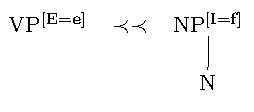
\includegraphics[scale=1]{NaTemp.pdf}
\end{minipage}
\caption{Time scale constructor: case of a scale with one marked point \label{constructor:time}}
\end{figure}

\begin{figure}
% \begin{minipage}{0.2\textwidth}
\avm{
\btag{f} [\type*{hurricane}
	   \TIME & \1\\
	   \LOC & \2\\
	   \NAME & \3
]
}
% \end{minipage}
\hfill%
% \begin{minipage}{0.55\textwidth}
\avm{
\btag{e} [\type*{event}
	\NOUNDIM & [ \type*{time $\und$ one-point-scale}
			\MARKED & \1
	 ]
]
}
% \end{minipage}
\hfill%
% \begin{minipage}{0.2\textwidth}
\avm{
\btag{f} [\type*{hurricane}
	   \TIME & \1\\
	   \LOC & \2\\
	   \NAME & \3
]
}
% \end{minipage}
\caption{Frame representations of the noun \textit{uragan} `hurricane': dictionary entry on the left and the result of the unification with the time scale constructor on the right \label{frame:hurricane}}
\end{figure}

If the enriched noun representation is combined with the representation of the verb \textit{pere\v{z}it'} `to outlive', the resulting frame describes a bounded process of living of the (yet unspecified) actor that started before the hurricane time and ended after it. This frame is shown on \figref{frame:outlive:hurricane}. As in the case of crossing the road, the hurricane is not an argument of the verb and the two frames are only connected via the identity of the values of the attributes \NOUNDIM.

\begin{figure}
\begin{minipage}{0.75\textwidth}
\avm{
\btag{e} [\type*{bounded-event $\und$ process $\und$} \type*{proper-scale $\und$ one-marked-point $\und$ time}
	\MANN & [\type*{live}]\\
    \ACTOR & \tag{0}\\
    \VERBDIM & \btag{e}\\
  	\NOUNDIM & \btag{e}\\
    \MARKED & \2\\
    \INIT & [\type*{stage}
       \POS & \1 ]\\
     \FIN & [\type*{stage}
       \POS & \3 ]\\
  ]
}
\end{minipage}\hfill%
\begin{minipage}{0.2\textwidth}\centering
\avm{
\btag{f} [\type*{hurricane}
	   \TIME & \2\\
	   \LOC & \5\\
	   \NAME & \6\\
]
}\\
\svar{1} $<$ \svar{2} $<$ \svar{3}\\
\end{minipage}
\caption{Frame representation of the verbal phrase \textit{pere\v{z}it' uragan} `to survive the hurricane': dictionary entry on the left and enriched representation on the right \label{frame:outlive:hurricane}}
\end{figure}

The extraction of the marked point on the time scale can be also performed with nouns that lack explicit time points, such as person names, e.g., \textit{Ma\v{s}a} `Masha'. Of course, such extraction requires a more complex procedure that cannot be described in detail here, but the idea is that some significant point related to the event type denoted by the verb is extracted using a special constructor. In case of the event of living and a person \textit{Ma\v{s}a} `Masha' this point should be the time of Masha's death. To obtain is, one can use the constructor that creates a representation of the event of living of Masha from the representation of the name \textit{Ma\v{s}a} (using the representation of the derivational base for the \textit{pere-}prefixed verb, so in our case the frame on \figref{frame:live}). The tentative result of an application of such a constructor is shown on \figref{frame:Masha:live}.

\begin{figure}
\centering
\avm{
\btag{e} [\type*{process}
    \MANN & [\type*{live}]\\
    \ACTOR & [\type*{Masha}]\\
    \NOUNDIM & [\type*{time}
		\MARKED & \2    
    ]\\
    \VERBDIM & \btag{e}\\
    \MDIM & \btag{e}\\
    \MIN & \1\\
    \MAX & \2
  ]
}
\caption{Frame representation of the referent of the name \textit{Ma\v{s}a}, coerced into event interpretation using the verb \textit{\v{z}it'} `to live' \label{frame:Masha:live}}
\end{figure}

Now let us combine the frame representation of the verb \textit{pere\v{z}it'} `to outlive' and the representation of \textit{Ma\v{s}a} interpreted as an event of living of Masha that provides as a marked point Masha's time of death. Let us also fill the \ACTOR slot with the referent of the name \textit{Vasya}. With this, we obtain the frame representation of the tenseless variant of the phrases \textit{Vasja pere\v{z}il/pere\v{z}iv\"{e}t Ma\v{s}u} `Vasya outlived/will outlive Masha'. This representation is provided on \figref{frame:Vasja:outlive:Masha} and contains the following information: the sentence describes a bounded event \btag{e} of living of Vasya. There is another event \btag{f} of living of Masha, that is not central but is used for the comparison. The main event \btag{e} started at the time prior to the maximum point of living of Masha (point of Masha's death) and ended or will end at the time after the time of Masha's death. The relation between the time of Vasya's life and the time of Masha's birth is not specified.

\begin{figure}
\begin{minipage}{0.6\textwidth}
\avm{
\btag{e} [\type*{bounded-event $\und$ process $\und$} \type*{proper-scale $\und$ one-marked-point}
	\MANN & [\type*{live}]\\
    \ACTOR & [\type*{Vasya}]\\
    \VERBDIM & \btag{e}\\
  	\NOUNDIM & \btag{e}\\
    \MARKED & \2\\
    \INIT & [\type*{stage}
       \POS & \1 ]\\
     \FIN & [\type*{stage}
       \POS & \3 ]\\
  ]
}
\end{minipage}\hfill%
\begin{minipage}{0.35\textwidth}\centering
\avm{
  \btag{f} [\type*{process}
    \MANN & [\type*{live}]\\
    \ACTOR & [\type*{Masha}]\\
    \NOUNDIM & \btag{e}\\
    \VERBDIM & \btag{e}\\
    \MDIM & \btag{e}\\
    \MIN & \5\\
    \MAX & \2
  ]
}\\
\svar{1} $<$ \svar{2} $<$ \svar{3}
\end{minipage}
\caption{Frame representation of the tenseless variant of the phrases \textit{Vasja pere\v{z}il/pere\v{z}iv\"{e}t Ma\v{s}u} `Vasya outlived/will outlive Masha'  \label{frame:Vasja:outlive:Masha}}
\end{figure}

To complete the picture, let us consider the verb \textit{igrat'} `to play'. This verb does not provide a preselected measure dimension, so there is some freedom with respect to the selection of a relevant parameter of the direct object. The frame for the verb \textit{igrat'} `to play' is shown on the left side of \figref{frame:outplay}. 

When the representation of the verb \textit{igrat'} is combined with the representation of the prefix \textit{pere-} that is compatible with a marked point  scale, we obtain the frame shown on the right side of \figref{frame:outplay} that represents the semantics of the verb \textit{pereigrat'} `to outplay': a bounded event of \MANN \textit{play} that ends at a point of the scale above the marked point. 

\begin{figure}\small
\begin{minipage}{0.3\textwidth}
\avm{
\btag{e} [\type*{activity}
    \MANN & [\type*{play}]\\
    \ACTOR & \1\\
    \VERBDIM & \btag{e}
  ]
}
\end{minipage}\hfill%
\begin{minipage}{0.65\textwidth}\centering
\avm{
\btag{e} [\type*{bounded-event $\und$ activity}
  	\NOUNDIM & \4\\
  	\MANN & [\type*{play}]\\
    \ACTOR & \6\\
    \VERBDIM & \btag{e}\\
    \MDIM & \4 [
       \type*{proper-scale $\und$ one-marked-point}
       \MARKED & \2 ]\\
    \INIT & [\type*{stage}
       \POS & \1 ]\\
     \FIN & [\type*{stage}
       \POS & \3 ]\\
  ]
}\\
\svar{1} $<$ \svar{2} $<$ \svar{3}
\end{minipage}
\caption{Frame representations of the verbs \textit{igrat'} `to play' (left) and \textit{pereigrat'} `to outplay' (right) \label{frame:outplay}}
\end{figure}

The type of the scale and the marked point remain underspecified and need to be identified using the information about the direct object. I propose to use the same strategy as above: if the direct object is a referent of the name \textit{Ma\v{s}a}, the dimension constructor is based on the frame for the verb \textit{igrat'} `to play' to obtain an event of Masha playing that has some parameters, such as duration of the play or the quality of the play. As we have discussed in Section~\ref{subsection:semantics:pere}, such sentences as \textit{Vasja pereigral Ma\v{s}u} `Vasya outplayed Masha' are ambiguous and hard to interpret without the context that would provide the relevant parameter. The representations that can be obtained as a result of such complex scale extraction procedure are shown on \figref{frame:Masha:play}: the time-related interpretation on the left side and the quality-related interpretation on the right side.

\begin{figure}
\begin{minipage}{0.45\textwidth}
\avm{
\btag{e} [\type*{activity}
    \NOUNDIM & [\type*{time}
		\MARKED & \2    
    ]  ]
}\\

\avm{
\btag{f} [\type*{activity}
    \MANN & [\type*{play}]\\
    \ACTOR & [\type*{Masha}]\\
    \VERBDIM & \btag{f}\\
    \DURATION & \2\\
    \QUALITY & \3
  ]
}\\
\end{minipage}
\hfill
\begin{minipage}{0.45\textwidth}
\avm{
\btag{e} [\type*{activity}
    \NOUNDIM & [\type*{quality}
		\MARKED & \3    
    ]
  ]
}\\
\avm{
\btag{f} [\type*{activity}
    \MANN & [\type*{play}]\\
    \ACTOR & [\type*{Masha}]\\
    \VERBDIM & \btag{f}\\
    \DURATION & \2\\
    \QUALITY & \3
  ]
}
\end{minipage}
\caption{Frame representations of the referent of the name \textit{Ma\v{s}a}, coerced into event interpretation using the verb \textit{igrat'} `to play' and then enriched with measure dimension information \label{frame:Masha:play}}
\end{figure}

On the last step one of these representations gets combined with the frame for the verb \textit{pereigrat'} `to outplay' (let us take the quality interpretation) and the resulting frame denotes an event of playing by some \ACTOR  where the end of the playing event is associated with a higher value on the quality scale than the marked point that is the quality of Masha's playing.

\begin{figure}
\begin{minipage}{0.55\textwidth}
\avm{
\btag{e} [\type*{bounded-event $\und$ activity}
  	\NOUNDIM & \4\\
  	\MANN & [\type*{play}]\\
    \ACTOR & \6\\
    \VERBDIM & \btag{e}\\
    \MDIM & \4 [
       \type*{proper-scale $\und$} \type*{one-marked-point} \type*{$\und$ quality}
       \MARKED & \2 ]\\
    \INIT & [\type*{stage}
       \POS & \1 ]\\
     \FIN & [\type*{stage}
       \POS & \3 ]\\
  ]
}
\end{minipage}\hfill%
\begin{minipage}{0.4\textwidth}\centering
\avm{
\btag{f} [\type*{activity}
    \MANN & [\type*{play}]\\
    \ACTOR & [\type*{Masha}]\\
    \VERBDIM & \btag{f}\\
    \DURATION & \5\\
    \QUALITY & \2
  ]
}\\
\svar{1} $<$ \svar{2} $<$ \svar{3}
\end{minipage}
\caption{Frame representation of the verbal phrase \textit{pereigrat' Ma\v{s}u} `to outplay Masha' \label{frame:outplay:Masha}}
\end{figure}

\subsection{Iterative interpretation}
The last usage of the prefix \textit{pere-} that I provide a frame for is iterative and arises when the measure dimension of the event denoted by the derivational base is of type \textit{property-scale}. This event then becomes a value of the preparatory phase attribute of the new event. The initial and the final stages, the noun dimension, the measure dimension, and the manner attributes are copied to the event node that refers to the new event. 

\begin{figure}
\begin{minipage}{0.5\textwidth}
\avm{
\btag{f}  [\type*{bounded-event}
     \MDIM & \3 [\type*{property-scale} ]\\
     \NOUNDIM & \4\\
     \INIT &  \1\\
     \FIN &  \2 \\
     \MANN & \5\\
     \PREP & \btag{e} [\type*{event}
  	 	\THEME & \6\\
        \MDIM & \3\\
    	\NOUNDIM & \4\\
    	\INIT &  \1\\
     	\FIN &  \2 \\
     	\MANN & \5
     ]
  ]
 }
 \end{minipage}\hfill%
 \begin{minipage}{0.45\textwidth}
 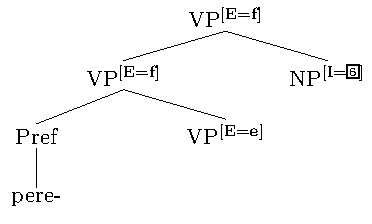
\includegraphics[scale=.85]{PereV.pdf}
 \end{minipage}
\caption{Representation of the contribution of the prefix \textit{pere-}: case of a property scale \label{frame:pere:iter}}
\end{figure}

The next restriction, apart from the property type of the scale, is that the event denoted by the derivational base must have a final stage in its representation. This means that a simplex imperfective verb cannot be combined with this prefix usage, unless it is coerced into a bounded event. On the formal side it means that we need a way to formulate the requirement on the frame (presence of the \FIN attribute). For implementing the coercion of an unbounded event into a bounded event I propose to use the frame shown on \figref{frame:coerce}. On the syntactic side it is accompanied by the introduction of an extra VP node.

\begin{figure}
% \begin{minipage}{0.7\textwidth}
\hfill%
\avm{
\btag{e}  [\type*{bounded-event}
     \MDIM & \3 [\type*{property-scale $\und$ closed-scale} 
		\MIN & \1\\
		\MAX & \2      
      ]\\
     \NOUNDIM & \3\\
     \INIT &  [\type*{stage}
     	\POS & \1]\\
     \FIN &  [\type*{stage}
     	\POS & \2]\\
  ]
 }\hfill%
%  \end{minipage}
%  \begin{minipage}{0.25\textwidth}
 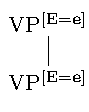
\includegraphics[scale=1]{VPcoerce.pdf}\hfill
%  \end{minipage}
\caption{Frame and tree for coercion of an unbounded event into a bounded event \label{frame:coerce}}
\end{figure}

\begin{figure}
\centering
\avm{
\btag{e} [\type*{bounded-event $\und$ activity}
	\MANN & [\type*{play}]\\ 
	\ACTOR & \4\\
    \VERBDIM & \btag{e}\\
     \MDIM & \3 [\type*{property-scale $\und$ closed-scale} 
		\MIN & \1\\
		\MAX & \2      
      ]\\
     \NOUNDIM & \3\\
     \INIT &  [\type*{stage}
     	\POS & \1]\\
     \FIN &  [\type*{stage}
     	\POS & \2]\\
  ]
}
\caption{Frame of the verb \textit{igrat'} `to play', coerced into a bounded event interpretation \label{frame:igrat:coerce}}
\end{figure}

Now if we take an imperfective verb, such as \textit{igrat'} `to play', and first coerce it using the frame on \figref{frame:coerce} (this operation is performed in the metagrammar and its result is shown on \figref{frame:igrat:coerce}) and then attach the prefix \textit{pere-} with the semantic representation shown on \figref{frame:pere:iter}, we obtain the frame shown on \figref{frame:pere:igrat}. This frame describes a bounded event of manner \textit{play} that is measured along the property scale, the initial stage being located at the minimum of the scale and the final stage being located at the maximum of the scale. In addition, there is a preparatory phase that refers to another event with similar characteristics.

\begin{figure}
\centering
\avm{
\btag{f} [\type*{bounded-event}
  		 \ACTOR & \4\\
  		 \THEME & \7\\
     	\MDIM & \3  [\type*{property-scale $\und$ closed-scale} 
			\MIN & \1\\
			\MAX & \2      
      	]\\
     	\NOUNDIM & \3\\
     	\INIT &  [\type*{stage}
     		\POS & \1
     	]\\
     	\FIN &  [\type*{stage}
     		\POS & \2
     	]\\
     	\MANN & [\type*{play}]\\
     	\PREP & \btag{e}  [\type*{bounded-event}
     		\ACTOR & \6\\
     		\THEME & \7\\
     		\MDIM & \3\\
     		\NOUNDIM & \3\\
      		\MANN & [\type*{play}]\\
     		\INIT &  [\type*{stage}
     			\POS & \1
     		]\\
     		\FIN &  [\type*{stage}
     			\POS & \2
     		]\\
    		\VERBDIM & \btag{e}
  		]
  ]
 }
\caption{Frame representation of the verb \textit{pereigrat'} `to replay' \label{frame:pere:igrat}}
\end{figure}

When the verb \textit{pereigrat'} `to replay' is used, an appropriate noun, probably unified with some dimension constructor, should occupy the position of the theme and contribute additional information about the scale. Let us take the noun \textit{partija} `match' that is probably characterized by duration, the type of the game it is a match of, and the set of players (see the left side of \figref{frame:match}). We are interested in particular in the \DURATION attribute as it is the only parameter that can bind the event. As we have already seen before, this attribute can be used to enrich the representation with the measure dimension information, as shown on \figref{frame:match}.

\begin{figure}\small
% \begin{minipage}{0.4\textwidth}
\avm{
\btag{g} [\type*{match}
	   \DURATION & \1\\
	   \GAME & [\type*{game}]\\
	   \PLAYERS & [\type*{entity}
	   		\CARD & \2
	   ] 
]
}\hfill%
% \end{minipage}
% \begin{minipage}{0.55\textwidth}
\avm{
\btag{f}[\type*{event}
 \NOUNDIM & [ \type*{time $\und$ closed-scale} \type*{$\und$ measure-of-change}
			\MIN & 0\\
			\MAX & \1
	   ]
]
}
% \end{minipage}
\caption{Frame representations of the noun \textit{partija} `match' (left) and of an additional component that is obtained as a result of its unification with the dimension constructor (right) \label{frame:match}}
\end{figure}

As a final step, we can now combine the frames on \figref{frame:pere:igrat} and on \figref{frame:match} and obtain the frame shown on \figref{frame:pere:igrat:match}. This frame describes a bounded event of playing that is preceded with another such event and both events are measured out according to the duration of the match. 

\begin{figure}\small
\avm{
\btag{f} [\type*{bounded-event}
  		 \ACTOR & \4\\
     	\MDIM & \3  [\type*{property-scale $\und$ closed-scale $\und$ time $\und$ measure-of-change} 
			\MIN & 0\\
			\MAX & \2   
      	]\\
     	\NOUNDIM & \3\\
     	\INIT &  [\type*{stage}
     		\POS & \1
     	]\\
     	\FIN &  [\type*{stage}
     		\POS & \2
     	]\\
     	\MANN & [\type*{play}]\\
     	\PREP & \btag{e} [\type*{bounded-event}
     		\ACTOR & \6\\
     		\THEME & \btag{g} [\type*{match}
	   			\DURATION & \2\\
	   			\GAME & [\type*{game}]\\
	   			\PLAYERS & [\type*{entity}
	   				\CARD & \7
	   			]
	   		]\\
     		\MDIM & \3\\
     		\NOUNDIM & \3\\
      		\MANN & [\type*{play}]\\
     		\INIT &  [\type*{stage}
     			\POS & \1
     		]\\
     		\FIN &  [\type*{stage}
     			\POS & \2
     		]\\
    		\VERBDIM & \btag{e}
  		]
  ]
 }
\caption{Frame representation of the verbal phrase \textit{pereigrat' partiju} `to replay the match' \label{frame:pere:igrat:match}}
\end{figure}

\clearpage

\section{Frame semantics for the prefix \textit{do-}}\label{section:frame:do}
The last prefix I will provide a frame for is the prefix \textit{do-}. As we have discussed in Chapter~\ref{Chapter5}, primarily following \citet{Kagan:book}, this prefix has completive or additive semantics: it can refer to the terminal part of the event or an event that can be seen as a continuation of another event. In Section~\ref{subsection:semantics:do} I came to the following conclusions with respect to the selection of the scale for the measure dimension: the first choice is the pre-specified verbal scale, next comes the scale extracted from the representation of the noun, and the last option is the event scale. 

This scheme can be realized by identifying the values of the measure dimension and the noun dimension attributes and adding an extra rule that would equate the verbal dimension with the measure dimension for intransitive verbs. When the prefix is attached, the maximum of the scale has to be associated with the final stage of the event. The frame that realizes these ideas is shown on \figref{frame:do}. Note that attributes in Frame Semantics are functional, so the attribute \PARTOF has to satisfy this restriction as well. To ensure this, I propose to define the value of this attribute as  the maximum event that the event in question is part of. In particular, it would be an event that proceeds from the minimum to the maximum degree on the relevant scale (provided by the \MDIM attribute). The scale has to be closed in order for the value of the \PARTOF attribute to be defined.

\begin{figure}
\begin{minipage}{0.45\textwidth}
\avm{
\btag{f} [\type*{bounded-event}
   		\MANN & \4\\
   		\ACTOR & \5\\
  	 	\THEME & \9\\
        \MDIM & [ \type*{closed-scale $\und$} \type*{property-scale}
			\MIN & \2\\
			\MAX & \1						
        ]\\
    	\INIT & [\type*{stage}
    		\POS &  \3]\\
     	\FIN &  [\type*{stage}
    		\POS &  \1]\\
     	\PARTOF & \btag{e}\\
       \NOUNDIM & [\7]\\
       \VERBDIM & [\8]
    ]
 }
 \end{minipage}\hfill%
 \begin{minipage}{0.45\textwidth}\centering
\avm{
\btag{e} [\type*{bounded-event}
   		\MANN & \4\\
   		\ACTOR & \6\\
  	 	\THEME & \9\\
        \MDIM & [ \type*{closed-scale $\und$} \type*{property-scale}
			\MAX & \1						
        ]\\
    	\INIT &  [\type*{stage}
    		\POS &  \2]\\
     	\FIN &  [\type*{stage}
    		\POS &  \1]\\
       \NOUNDIM & [\7]\\
       \VERBDIM & [\8]
    ]
 }\\
$\tuple{\btag{f}\BC\MDIM,\btag{e}\BC\MDIM}\D\type{segm-of}$\\[1ex]
\end{minipage}
\caption{Frame representation of the prefix \textit{do-} \label{frame:do}}
\end{figure}

Similarly to the iterative usage of the prefix \textit{pere-}, the prefix \textit{do-} can be only attached to bounded events. This means that, again, simplex imperfective verbs need to be first coerced into a bounded interpretation. For coercion I propose to use the same frame as we have used before when combining the verbs with the prefix \textit{pere-}: coercion frame shown on \figref{frame:coerce}. As we have already performed coercion for the verb \textit{igrat'} `to play', let us see how the prefix \textit{do-} attaches to this verb. For this, we take the frame on \figref{frame:do} and use the frame on \figref{frame:igrat:coerce} as a base event identified as \btag{e} in the frame on \figref{frame:do}. As a result we obtain the frame shown on \figref{frame:do:igrat} that refers to a bounded event that is part of another event. The scale of the new event is also a part of the scale of the event denoted by the derivational base. 

\begin{figure}\small
 \begin{minipage}{0.45\textwidth}
\avm{
\btag{f} [\type*{bounded-event}
   		\MANN & \4\\
   		\ACTOR & \5\\
  	 	\THEME & \8\\
        \MDIM & [\type*{property-scale} \type*{$\und$ closed-scale} 
			\MIN & \2\\
			\MAX & \1						
        ]\\
    	\INIT &  [\type*{stage}
    		\POS &  \3]\\
     	\FIN &  [\type*{stage}
    		\POS &  \1]\\
     	\PARTOF & \btag{e}\\
       \NOUNDIM & [\type*{property-scale} \type*{$\und$ closed-scale}]\\
       \VERBDIM & [\type*{bounded-event} \type*{$\und$ activity}]
    ]
 }
 \end{minipage}\hfill%
  \begin{minipage}{0.45\textwidth}\centering
 \avm{
\btag{e} [\type*{bounded-event} \type*{$\und$ activity}
	\MANN & [\type*{play}]\\ 
	\ACTOR & \6\\
  	 \THEME & \8\\
    \VERBDIM & \btag{e}\\
     \MDIM & \3 [\type*{property-scale} \type*{$\und$ closed-scale} 
		\MIN & \2\\
		\MAX & \1      
      ]\\
     \NOUNDIM & \3\\
     \INIT &  [\type*{stage}
     	\POS & \2]\\
     \FIN &  [\type*{stage}
     	\POS & \1]\\
  ]
}\\
$\tuple{\btag{f}\BC\MDIM,\btag{e}\BC\MDIM}\D\type{segm-of}$\\[1ex]
\end{minipage}
\caption{Frame representation of the verb \textit{doigrat'} `to finish playing' \label{frame:do:igrat}}
\end{figure}

To make clear why the complicated rules of how the measure dimension is constructed are needed, let me show what happens when the direct object comes into play and how the verb prefixed with \textit{do-} once differs from the verb prefixed with the same prefix twice. The frame on \figref{frame:do:igrat:partiju} shows the representation of the phrase \textit{doigrat' partiju} `to finish playing the match', formed using the frame on \figref{frame:do:igrat} and the frame on the right side of \figref{frame:match}. It is important to note that the information that comes from the direct object is unified at the deepest relevant level: this means that for a non-suffixed verb with multi-event representation it would be always the representation of the event denoted by the base verb. In case of the prefix \textit{pere-}, despite the multi-layer representation, this did not play a role, as all the information is passed to the higher layer without changes. Here, however, the \THEME is identical for the partial event and the whole event, but the noun dimension of the new event only inherits the type of the scale and not the values of the extreme points. Instead, a new scale of the same type, but probably with a different \MIN point, is constructed.

\begin{figure}\small
\avm{
\btag{e} [\type*{bounded-event}
   		\MANN & \7 [\type*{play}]\\
   		\ACTOR & \5\\
  	    \THEME & \8\\
        \MDIM & [\type*{property-scale $\und$ closed-scale} 
			\MIN & \2\\			
			\MAX & \1						
        ]\\
    	\INIT &  [\type*{stage}
    		\POS &  \3]\\
     	\FIN &  \6\\
     	\PARTOF & \btag{e}\\
       \NOUNDIM & [\type*{property-scale $\und$ closed-scale}]\\
       \VERBDIM & [\type*{bounded-event $\und$ activity}]
    ]
 }\medskip\\
 \avm{
\btag{e} [\type*{bounded-event $\und$ activity}
	\MANN & \7\\ 
  	 \THEME & \8[\type*{match}
	   \DURATION & \1\\
	   \GAME & [\type*{game}]\\
	   \PLAYERS & [\type*{entity}
	   		\CARD & \2
	   ]\\
	   \NOUNDIM & \3
	]\\
	\ACTOR & \9\\
    \VERBDIM & \btag{e}\\
     \MDIM & \3 [\type*{time $\und$ measure-of-change $\und$ property-scale $\und$ closed-scale} 
		\MIN & 0\\
		\MAX & \1     
      ]\\
     \NOUNDIM & \3\\
     \INIT &  [\type*{stage}
     	\POS & \2]\\
     \FIN &  \6 [\type*{stage}
     	\POS & \1]\\
  ]
}\\
$\tuple{\btag{f}\BC\MDIM,\btag{e}\BC\MDIM}\D\type{segm-of}$\\[1ex]
\caption{Frame representation of the verbal phrase \textit{doigrat' partiju} `to finish playing the match' \label{frame:do:igrat:partiju}}
\end{figure}

As one can see on \figref{frame:do:igrat:partiju}, in this case the measure dimension of the partial event is the same as the measure dimension of the whole event. It is different when two prefixes are stacked, as in the verb \textit{dodoigrat'} `to finish playing the final part'. One would like to see a different semantic representation in this case, while otherwise such verb could not be used, as it would violate the pragmatic principles. Under the analysis I propose here, the verbal phrase \textit{dodoigrat' partiju} `to finish playing the final part of the match' receives the frame representation shown on \figref{frame:do:do:igrat:partiju} (this frames makes reference to the frame shown on \figref{frame:do:igrat:partiju}). So the event denoted by the verbal phrase \textit{dodoigrat' partiju} `to finish playing the final part of the match' is an event of playing that does not necessarily start from the minimum of the scale and the minimum of the scale is not bound to the beginning of the match. Such a frame still allows the interpretation that the new event refers to an event of playing the whole match, but this will be blocked by pragmatic reasoning.

\begin{figure}
\avm{
\btag{g} [\type*{bounded-event}
   		\MANN & \7 [\type*{play}]\\
   		\ACTOR & \4\\
  	    \THEME & \8\\
        \MDIM & [\type*{time $\und$ measure-of-change $\und$ property-scale $\und$ closed-scale} 
			\MIN & \3\\			
			\MAX & \1						
        ]\\
    	\INIT &  [\type*{stage}
    		\POS &  \tag{10}]\\
     	\FIN &  \6 [\type*{stage}
    		\POS &  \1]\\\\
     	\PARTOF & \btag{f}\\
       \NOUNDIM & [\type*{property-scale $\und$ closed-scale}]\\
       \VERBDIM & [\type*{bounded-event $\und$ activity}]
    ]
 }\\
$\tuple{\btag{g}\BC\MDIM,\btag{f}\BC\MDIM}\D\type{segm-of}$\\[1ex]
\caption{Frame representation of the verbal phrase \textit{dodoigrat' partiju} `to finish playing the final part of the match': additional component with respect to \figref{frame:do:igrat:partiju} \label{frame:do:do:igrat:partiju}}
\end{figure}

Let me show what happens when the prefix \textit{do-} is attached to a verb that has a pre-selected measure dimension. Consider a determinate motion verb \textit{be\v{z}at'} `to run' that we have used earlier in combination with the prefix \textit{pere-} (see \figref{frame:bezhat}). The basic verb \textit{be\v{z}at'} `to run' also has to be coerced before prefixation, so instead of doing this step (that would be similar to the procedure above, illustrated by the verb \textit{igrat'} `to play'), let us take as an input the prefixed verb \textit{perebe\v{z}at'} `to cross'. The result of combining the frame representation of the verb \textit{perebe\v{z}at'} `to cross' (right side of \figref{frame:bezhat}) with the frame representation of the prefix \textit{do-}, shown on \figref{frame:do}, is provided on \figref{frame:do:perebezhat}. This verb denotes an event that is a part of an event of crossing the road and necessarily includes the final part of the crossing. 

\begin{figure}
\begin{center}
\avm{
\btag{f} [\type*{bounded-event $\und$ transloc}
   		\MANN & [\type*{run}]\\
   		\ACTOR & \5\\
        \MDIM & \7 [ \type*{path $\und$ closed-scale $\und$ proper-scale}
			\MIN & \2\\
			\MAX & \1						
        ]\\
    	\INIT &  [\type*{stage}
       		\POS & \3 ]\\
     	\FIN &  \8 \\
     	\PARTOF & \tag{0}\\
       \NOUNDIM & \7\\
       \VERBDIM & \7 [ \type*{path $\und$ closed-scale $\und$ property-scale}]
    ]
 }\\
 \vspace{1em}
\avm{
\btag{e} [\type*{bounded-event $\und$ transloc}
	   	\MANN & [ \type*{run} ]\\
       	\ACTOR & \6\\
	   \PATH & [\type*{path}]\\
	   	\TRACE & [ \type*{trace} ]\\
	   	\VERBDIM & \4 \\
	   	\MDIM & \4 [ \type*{path $\und$ closed-scale $\und$ proper-scale}
       		\MIN & \9\\
       		\MAX & \1
       	]\\
      	\NOUNDIM & \4\\
    	\INIT & [\type*{stage}
       		\POS & \9 ]\\
     	\FIN & \8 [\type*{stage}
       		\POS & \1 ]
    ]
 }\\
 $\tuple{\btag{f}\BC\MDIM,\btag{e}\BC\MDIM}\D\type{segm-of}$\\[1ex]
 \end{center}
\caption{Frame representation of the verb \textit{doperebe\v{z}at'} `to finish crossing' \label{frame:do:perebezhat}}
\end{figure}

%\section{Semantics for the imperfective suffix}
%\section{Compositional semantics}
%\section{Testing the predictions}
%
%
%
%\section{Metagrammar}
%Linguistic generalizations in TAGs are captured by a metagrammar. There are two steps of factorization, which are important for this paper:
%\begin{itemize}
%\renewcommand{\labelitemi}{$\bullet$}
%\item \textit{unanchored elementary trees} are specified separately from lexical anchors;
%\item trees are organized into \textit{tree families} which represent different realizations of one subcategorization frame.
%\end{itemize}
%This allows to define a meaning for sets of unanchored elementary trees, i.e., a meaning of constructions.
%
%\section{Morphological decomposition}\label{sec-morph}
%\section{Inducing aspectual properties from semantic representation}
%
%How to make sure we get the appropriate object: 
%As suggested by \citet{Rappaport:08}, ``scales require that the participant whose property is measured by them be overtly realized." I want to slightly modify this suggestion and claim that whenever a point on the scale is used to determine when the event terminates, this point cannot be related to an unbound variable. If no link between such point and the world has been specified, the whole derivation fails. 

\section{Summary}
In this chapter I have proposed frame representations of the semantic contribution of five Russian verbal prefixes: \textit{za-, na-, po-, pere-,} and \textit{do-}. We have seen that these representations are quite distinct: in case of the prefix \textit{za-} the derived verb refers to a transition that is connected with the event denoted by the derivational base via relations; the prefixes \textit{na-} and \textit{po-} both add information to the initial event frame, but differ with respect to the processes of dimension selection and assigning scale degrees to the initial and final stages of the event; the prefix \textit{pere-} creates a new event with a preparatory phase consisting of the event denoted by the derivational base; and the prefix \textit{do-} refers to a partial event that is constructed during the derivation with a probable change of the minimum point of the measure dimension scale.

We have also seen that in order to obtain the representation of the derived verb, several steps related to the scalar selection process have to be made. We need to select the dimension of the verb, the relevant dimension of the object, and find out the type of the scale that will be used for measuring the event. In some cases this scale is the event itself. 

As objects are often associated with different dimensions, I have proposed various constructors that allow to extract relevant information. Some of these constructors (e.g., temperature dimension constructor, \figref{constructor:temp}) can be applied without restrictions, some (e.g., amount dimension constructor, \figref{constructor:amount}) are accompanied by syntactic restrictions, and some (e.g., the constructor that reconstructs the event of living from the person's name) can be used only in special cases when the scalar interpretation is required and no other constructor can be applied. As modelling semantic representation and shifts of meaning of nouns is not the goal of this work, the proposed constructors will most probably require revisions, but they suffice to illustrate how the object can contribute to determining the interpretation of the prefixed verb.

The representations I have proposed here differ in their complexity: while frames for some prefixed verbs differ from the representations of the respective derivational bases only by the presence of several additional attributes (as in case of the prefixes \textit{po-} and \textit{na-}), frames for other prefixed verbs are a lot more complex (prefixes \textit{do-} and \textit{pere-}). A hypothesis that would be interesting to check empirically is whether in case of verbs that are represented using multi-layered frames the interpretation requires an increased amount of processing time relative to verbs with the same morphological complexity but less complex semantic representation.


In the next part, Chapter~\ref{Chapter8}, I will show how frame representations proposed in this chapter can be implemented using a metagrammar compiler.
 % Formal analysis 
% Chapter 8

\chapter{Implementation of the analysis using XMG} % Write in your own chapter title
\label{Chapter8}
%\lhead{Chapter 7. \emph{Implementation of analysis using XMG}} 
In Chapter~\ref{Chapter7} I have proposed a frame \isi{semantic analysis} of various prefixes together with selected pieces of the \isi{syntax-semantics interface}. In this chapter I present the implementation of the proposal.

 In order to describe and provide a compact grammar description, one can use a \isi{metagrammar} compiler. A TAG \isi{metagrammar} is a reduced description that captures linguistic generalisations that appear in the trees that belong to the grammar \citep{Candito:99}. EXtensible MetaGrammar\footnote{\url{http://xmg.phil.hhu.de/}} \citep[\isi{XMG},][]{Crabbe:13} is a formalism that allows to describe linguistic information contained in the grammar and a tool to compute grammar rules and produce a redundant strongly lexicalised TAG. 
 
Among the properties of \isi{XMG} that distinguish it from other grammar engineering environments, two are of particular importance for the current work. First, \isi{XMG} is a declarative language, which means that it is based on constraints and not on procedures. This allows for an order-independent definition of grammaticality. Second, \isi{XMG}'s notation is highly expressive: in particular, various linguistic dimensions are treated in a modular war, and grammatical units can be disjoint, conjoint, and inherited.
 
 \isi{XMG} 2 \citep{Petitjean:16} is a tool that is used to create \isi{metagrammar} compilers, adapting them to specific needs. Whereas \isi{XMG} supports three independent levels of description: \isi{syntactic trees} (syn), semantic predicate structures (sem), and dynamic interfaces between syn and sem (dyn), \isi{XMG} 2 allows to introduce additional dimensions. The compiler I am using for the current implementation is created using \isi{XMG} 2 and has a syntactic (syn) and a frame semantic (frame) dimension  \citep{Lichte:15}.

The syntactic dimension is described using the following elements: first, all the nodes are declared using the keyword \texttt{node} and a variable name. These declarations are accompanied by optional marks (in brackets) and syntactic features (in square brackets, separated by commas). Values of syntactic features can be either specified or represented by a variable to ensure the same value of the feature across the nodes without specifying it. Second, the relations between the nodes are stated. I will use the following relations ($x$ and $y$ range over node variables): $x \rightarrow y$ for the immediate dominance of the node $x$ over the node $y$; $x \rightarrow + y$ for the dominance (reflexive transitive closure of the immediate dominance relation) of the node $x$ over the node $y$; 
$x >> y$ for the immediate precedence of the node $x$; and $x >>+ y$ for the precedence (transitive closure of the immediate precedence relation) of the node $x$.

\isi{XMG} is designed to output unanchored TAG elementary trees, but as currently there is no parser that would take into account frame semantic dimension, I simulate the insertion of \isi{lexical anchors} in the \isi{metagrammar}. This solution leads to a more complicated \isi{metagrammar} architecture, but allows to see the results in a form that can be easily understood. If I were to output the unanchored trees only, I would obtain \isi{prefixation} schemes but the stem that carries important information would not be inserted, which would make is very hard to check the predictions. 

%On the other hand, I had to limit the size of the fragment for implementation, as together with all the lexical decisions the \isi{metagrammar} descriptions grows too fast and it becomes harder to maintain and test it. 

The implemented grammar fragment I want to show contains the following elements: a noun \textit{rasskaz} `story', a verb \textit{pisat'} `to write', a prefixed verb \textit{zapisat'} `to write down', prefixes \Prefix{po-} (\isi{delimitative} and \isi{distributive} interpretations), \Prefix{pere-} (\isi{repetitive} and \isi{distributive} interpretations), and \Prefix{do-}, and \isi{imperfective suffix} \textit{-iva-} (iterative and progressive interpretations).  With this inventory I construct verbs with a maximum of four affixes (can be realised if the a base verb is prefixed two times, then suffixed, and then prefixed again). This architecture in principle allows to construct more than 1000 verbal phrases, out of which the compiler outputs 88 models. Nine of those models have to be filtered out later by the pragmatic module, but those numbers show that most of the work is done by the constraints from the syntax-semantics part.

In this chapter I will show fragments of the implementation and explain decisions that I had to make. The whole code and the corresponding output of the compiler are provided in Section~\ref{B:me} of Appendix~\ref{AppendixB}. In the last section I will present an implementation of the analysis proposed in \citet{Tatevosov:09} (code provided in Section~\ref{B:Tat} of Appendix~\ref{AppendixB}) that is done using the same tools. I will then compare the outputs of two implementations. Both implementations and the xml files that are output by the compiler are also available online\footnote{\url{https://user.phil-fak.uni-duesseldorf.de/~zinova/XMG/index.html}}.

\section{Type hierarchy and constraints}
The code starts with the three unicity constraints shown on \figref{xmg:unicity} that prevent the appearance of some features more than once in the same \isi{elementary tree}. The first constraint is a standard one, as it ensures that each tree has one \isi{lexical anchor}. The second constraint has to be introduced because I use \isi{XMG} not only for constructing the unanchored trees, but also for the insertion of the \isi{lexical anchors}. This constraint allows to make sure that only one noun is inserted in the accusative noun slot.

\begin{figure}
\begin{lstlisting}[style=xmg]
use unicity with (mark=anchor) dims (syn)
use unicity with (mark=nounacc) dims (syn)
use unicity with (iteration=yes) dims (syn)
\end{lstlisting}
\caption{XMG code: unicity constraints \label{xmg:unicity}}
\end{figure}

The third constraint restricts the appearance of the \textit{iteration} feature to one per tree. The nature of this constraint is semantic and the natural way would be to locate it in the semantic dimension. This is, however, not yet implemented, so I copy the feature to the syntactic level and apply the unicity constraint in the syntactic dimension.

The next three sections introduce syntactic features, types associated with values of these features, and frame types. Here I want to note two more features that I had to ``lift'' to the syntactic level due to the fact that such feature checking inside the semantic dimension of \isi{XMG} is not yet supported: \textit{bounded} and \textit{limited}. The feature \textit{bounded} appears at those nodes that are associated with frames of \textit{event} type. It gets the value \textit{yes} if there is a path from the central node of the frame to an attribute \FIN that can proceed through the \PARTOF attributes. If there is no such path, the value of the feature is \textit{no}. The feature \textit{limited} is a stronger version of a similar constraint: for \textit{limited} to get the value \textit{yes}, the central node has to have an attribute \FIN and its value has to be specific (concrete value or a bound variable). In all other cases the feature \textit{limited} gets value the \textit{no}.

We have discussed the crucial fragments of the \isi{type hierarchy} in Section~\ref{section:types}. Now all those restrictions plus some more constraints that are related to the nominal domain were left out from the previous discussion have to be formalised. Figure~\ref{xmg:types} shows a part of type constraints that states that \textit{length} is a type of \textit{scale}, in particular \textit{property-scale}. This type is not compatible with a \textit{cardinality} scale type which is always a \textit{closed-scale}. The rest of the hierarchy is written in a similar way.

\begin{figure}
\begin{lstlisting}[style=xmg]
property-scale -> scale,
length -> property-scale,
cardinality property-scale -> -,
closed-scale -> scale
cardinality -> closed-scale,
\end{lstlisting}
\caption{A fragment of type hierarchy \label{xmg:types}}
\end{figure}

\section{Lexical anchors}\largerpage[-1]
In a proper implementation that would separate the \isi{metagrammar} level from the syntactic level the following elements would not belong to the \isi{metagrammar}, but would be used as \isi{lexical anchors} for the appropriate tree families. The first entry is the noun that will be used to fill the object slot. I have selected the plural form of the noun \textit{rasskaz} `story' that has some length and also cardinality. The constraint on the unicity of the feature \textit{nounacc} that I have shown above is used here to prevent multiple insertions of the accusative noun \isi{lexical anchor}.

The description of the noun is straightforward: on the syntactic side, it is a daughter of the N category node and on the semantic side it contains relevant attributes. The two nodes (\texttt{?N} and \texttt{?Story}) are declared in the first two lines of the syntactic domain description and connected via an immediate dominance relation in the third line. Both nodes are characterised with feature \texttt{i=?X0} which connects them to the semantic frame characterised in the frame dimension. The frame description states that the type of the frame \texttt{?X0} is \texttt{story} and it has two attributes: The label of the central node of the frame (\texttt{?X0}) as well as the syntactic nodes and relevant dimension-related variables are exported for future use. 

The code for the class is shown on \figref{xmg:noun}. Note that I do not distinguish between top and bottom feature structures in the provided descriptions, as due to the absence of the \isi{adjunction} in the implemented fragment the division into top and bottom parts is not relevant. Figure~\ref{story:tree:frame} shows the tree and the frame that are described by the code for the class \texttt{Story} (features of the syntactic dimension are omitted).

\begin{figure}[p]
\begin{lstlisting}[style=xmg,basicstyle=\small\ttfamily]
class Story
export ?Length ?Card ?N
declare ?N ?Story ?X0 ?Length ?Card
{
  <syn>{
    node ?N (mark=coanchor) [cat=n, num = pl, i=?X0];
    node ?Story (mark=nounacc) [cat=rasskazy, num = pl, i=?X0];
    ?N -> ?Story
  };
  <frame>{
    ?X0[story,
        length: ?Length,
        cardinality: ?Card
    ]
  }
}
\end{lstlisting}
\caption{XMG code: noun that is used to fill the accusative NP slot \label{xmg:noun}}
\end{figure}

\begin{figure}[p]
\begin{minipage}{.5\textwidth}
\centering
% % 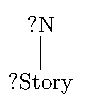
\includegraphics[scale=1]{StoryTree.pdf}
\begin{forest}
[?N [?Story]]
\end{forest}
\end{minipage}%
\begin{minipage}{0.5\textwidth}
\avm[types=\normalfont,values=\normalfont,attributes=\normalfont]{
?X0 [\type*{story}
      length & ?Length\\
      cardinality & ?Card
   ]}
\end{minipage}
\caption{Tree and frame representation of the code provided on \figref{xmg:noun}\label{story:tree:frame}}
\end{figure}\clearpage

Later this noun can enter one of the two \isi{dimension constructors}: length or cardinality. The \isi{cardinality constructor} code is shown on \figref{xmg:cardinality}. It should be available for all nouns that have a cardinality attribute with an additional restriction for plural number. The constructor creates a NP node that dominates the N node exported from the description of the noun, and a VP node that linearly precedes the NP node. The output of the class is a discontinuous tree, as shown by the tree on \figref{card:tree:frame}. On the semantic side an \MDIM attribute is created and the event description bounded to the VP node also acquires the type \textit{iteration}. This is, as announced before, doubled via the iteration attribute on the syntactic side. The frame described by the frame part of the code is provided on the right side of \figref{card:tree:frame}.

\vfil
\begin{figure}
\begin{lstlisting}[style=xmg,basicstyle=\small\ttfamily]
class NounCardinal
export ?N ?NP ?VP
declare ?NCard ?X0 ?Card ?N ?NP ?VP ?Dim ?Theme ?Case ?Num 
{
  ?NCard=Story[];
  ?NCard.?Card = ?Card;
  ?N=?NCard.?N;
    <syn>{
    node ?NP [cat=np, case=?Case, num = pl, i=?Theme];
    node ?VP [cat=vp, e=?X0, iteration = yes];
    node ?N (mark=coanchor) [cat=n, case = ?Case, num = pl, i=?Theme];
    ?VP >>+ ?NP;
    ?NP -> ?N
  };
  <frame>{
    ?X0[iteration,
        theme:?Theme,
        m-dim:[cardinality,
                min:[zero],
                max:?Card
        ]
    ]
  }
}
\end{lstlisting}
\caption{XMG code: constructor of the cardinality dimension \label{xmg:cardinality}}
\end{figure}
\vfil
\pagebreak

\begin{figure}
% \begin{minipage}{0.5\textwidth}
% % 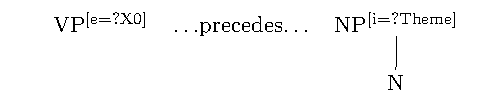
\includegraphics[scale=1]{NounCardTree.pdf}\\
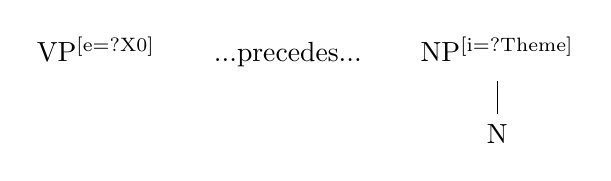
\begin{tikzpicture}[baseline]
\node at (0,0) (VP) {\strut VP\textsuperscript{[e=?X0]}};
\node [right=.5cm of VP] (precedes) {...precedes...};
\node [right=.5cm of precedes] (NP) {\strut NP\textsuperscript{[i=?Theme]}};
\node [below=\baselineskip of NP] (N) {N};
\draw (NP) -- (N);
\end{tikzpicture}\medskip\\
% \end{minipage}%
% \begin{minipage}{0.5\textwidth}
\avm[types=\normalfont,values=\normalfont,attributes=\normalfont]{
?X0 [\type*{iteration}
      theme & ?Theme\\
      m-dim & [\type*{cardinality}
      	min & [\type{zero}]\\
      	max & ?Card]
]
}
% \end{minipage}
\caption{Tree and frame representation of the code provided on \figref{xmg:cardinality}\label{card:tree:frame}}
\end{figure}

Another dimension constructor that I use, implemented in the class \texttt{NounLength},  is organised in a similar way with a difference that it creates a \NOUNDIM, not an \MDIM attribute of the event, is available for nouns that have a \LENGTH attribute independently of their number, and does not specify the event type.

\begin{figure}
\begin{lstlisting}[style=xmg,basicstyle=\small\ttfamily]
class Pisat
export ?V
declare ?V ?Pisat ?X0 ?Actor ?Theme ?Mean
{
  <syn>{
    node ?V (mark=anchor) [cat=v, e=?X0, asp = unbound, aspect = imperf];
    node ?Pisat (mark=flex) [cat=pisat, e=?X0, asp = unbound, 
    	aspect = imperf];
    ?V -> ?Pisat
  }
  ;
  <frame>{
    ?X0[event & process,
        actor:?Actor,
        theme:?Theme,
        mean:?Mean,
        manner:[write],
        verb-dim:?X0
    ]
  }
}
\end{lstlisting}
\caption{XMG code for representation of the verb \textit{pisat'} `to write' \label{xmg:pisat}}
\end{figure}

The second group of lexical items consists of two verbs: \textit{pisat'} `to write' and \textit{zapisat'} `to write down'. The second verb contains the prefix \Prefix{za-}, but its semantic contribution is not transparent, so the whole verb must be stored in the dictionary. The class that represents the verb \textit{pisat'} `to write' has a simple \isi{syntactic structure} of two nodes (see \figref{xmg:pisat}): the node of category V and the node that contains the verb itself, where the V node inherits all syntactic properties of the verb, except for the category. The \textit{aspect} feature, in contrast with the features \textit{limited} and \textit{bounded}, is a syntactic feature and carries information about the syntactic aspect of the verb represented by the respective node. For the frame semantic side, I use a simple representation that serves the purposes of the current analysis. I acknowledge that the fully elaborated representation may be more complex or just differ in details, but this should not influence the results of the current study.


The \isi{syntactic structure} of the prefixed verb \textit{zapisat'} `to write down/record' is more complex: the highest node is of category VP and under it a prefix node and another VP node are located. The \isi{internal} VP node (VPInt in the code) is needed to make the structure of the dictionary-stored prefixed verb similar to the structure of prefixed verbs assembled in the \isi{metagrammar}. On the semantic side this verb also differs from the verb \textit{pisat'} `to write' a lot: it includes information about the \isi{measure dimension} as well as about the initial and final stages of the event. The \isi{XMG} code of the class that represents the verb \textit{zapisat'} `to write down/record' is shown on \figref{xmg:zapisat} and the result of the compilation of the class is provided on \figref{fig:zapisat}.
 
 \begin{figure}
\begin{lstlisting}[style=xmg,basicstyle=\footnotesize\ttfamily]
class Zapisat
export ?VP ?VPInt ?VPBase
declare ?V ?Pisat ?Za ?ZaLex ?X0 ?Actor ?Theme ?ScMin ?ScMax ?AGR ?VP 
?VPInt ?VPBase
{
   ?VPBase = ?VPInt;
   <syn>{
    node ?VP [cat=vp, agr=?AGR, e=?X0, asp = bound, aspect = perf];
    node ?V (mark=anchor) [cat=v, agr=?AGR, asp = unbound, 
    	aspect = imperf];
    node ?Pisat (mark=flex) [cat=pisat, agr=?AGR, asp = unbound, 
    	aspect = imperf];
    node ?Za [cat=pref];
    node ?ZaLex (mark=flex) [cat=za-];
    node ?VPInt [cat=vp, agr=?AGR, e=?X0, aspect = perf, asp = bound];
    ?VP -> ?VPInt;
    ?VPInt -> ?V;
    ?VP -> ?Za;
    ?Za -> ?ZaLex;
    ?Za >> ?VPInt;
    ?V -> ?Pisat
  }
  ;
  <frame>{
    ?X0[bounded-event & process,
        actor:?Actor,
        theme:?Theme,
        manner:[record],
        verb-dim:?X0,
        noun-dim:[property-scale,
          min: ?ScMin,
          max: ?ScMax
        ],
        m-dim:[property-scale,
          min: ?ScMin,
          max: ?ScMax
        ],
        init: [stage, 
          scale-deg:?ScMin
        ],
        fin: [stage, 
          scale-deg:?ScMax
        ]
    ]
  }
}

\end{lstlisting}
\caption{XMG code for representation of the verb \textit{zapisat'} `to write down/record' \label{xmg:zapisat}}
\end{figure}

\begin{sidewaysfigure}
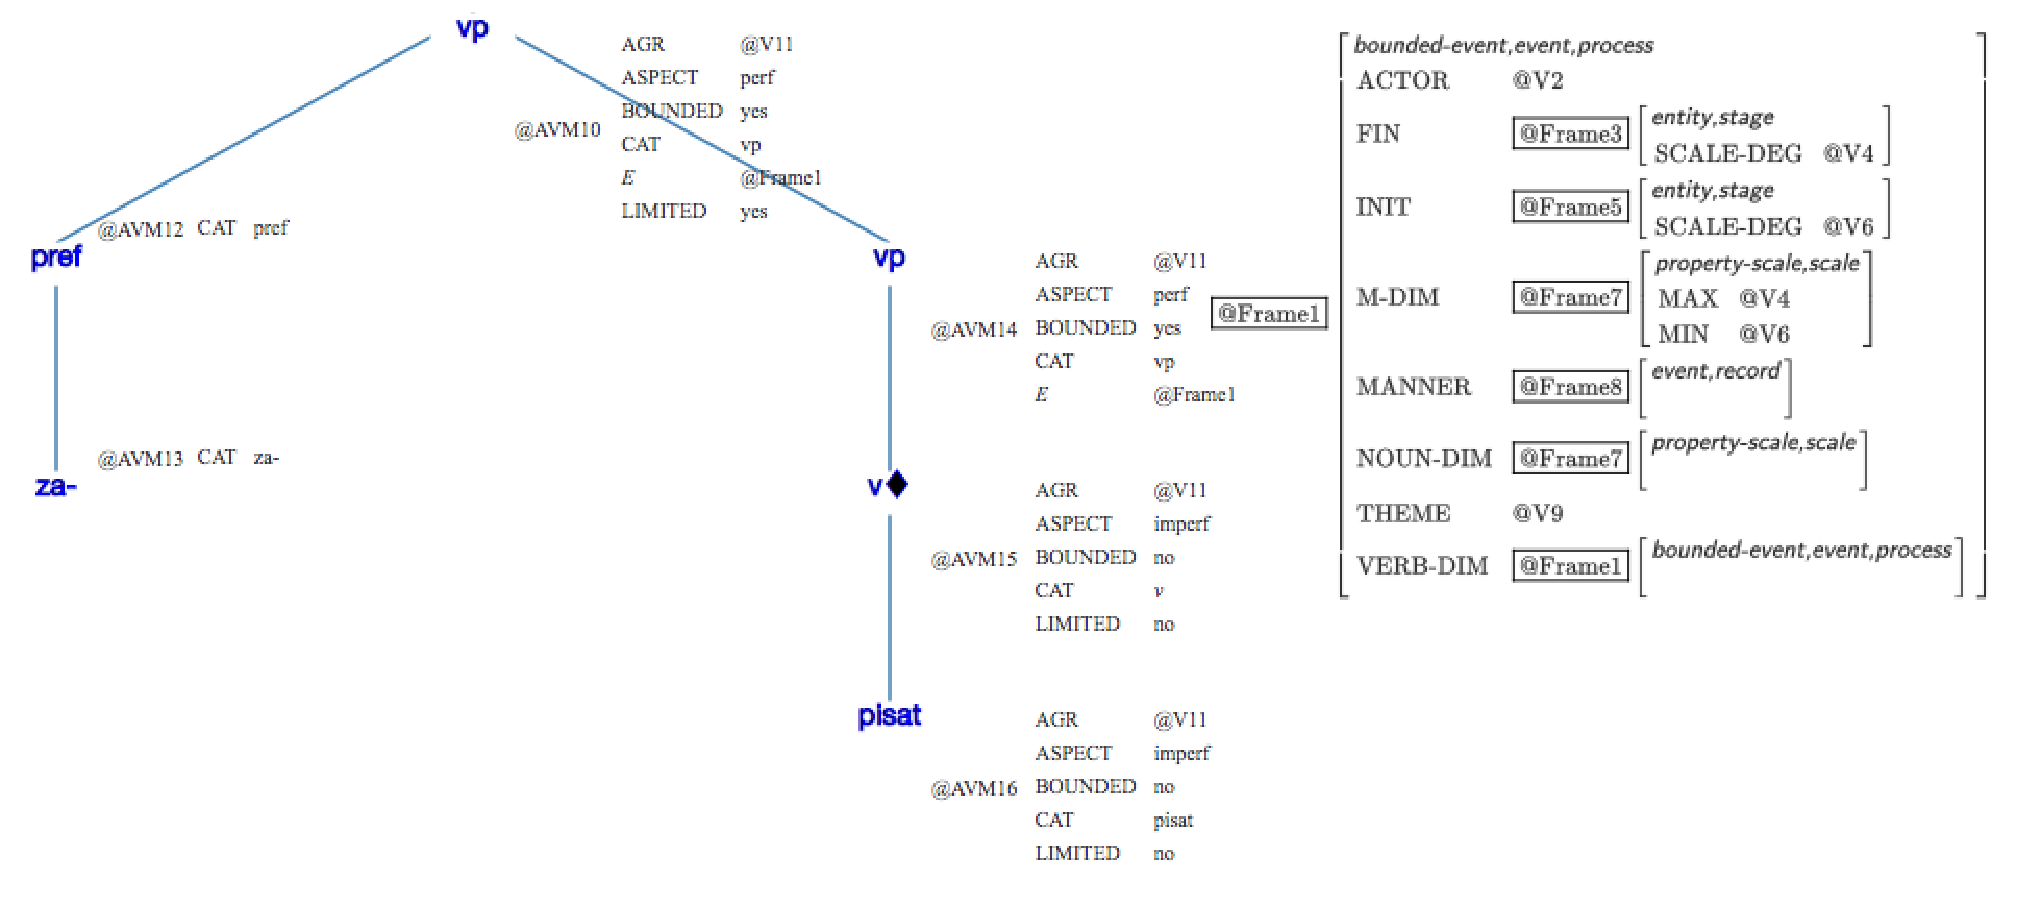
\includegraphics[width=\textwidth]{Zapisat.pdf}
\caption{Result of the compilation of the class \texttt{Zapisat}\label{fig:zapisat}}
\end{sidewaysfigure}

\section{Prefixes}
As we have already discussed the frames for all individual prefix usages in the previous chapter, I will not go through the code for all of them (it can be found in Appendix~\ref{AppendixB}), but show how frames correspond to the \isi{XMG} descriptions and what happens on the syntactic side, taking one prefix as an example.

Figure \ref{code:po} shows the \isi{XMG} description of the class for the prefix \Prefix{po-}. In this code, the syntactic part represents a VP that consists of a prefix head and another (\isi{internal}) VP that carries information about the \isi{derivational base}. The agreement information as well as the semantic frame are then passed to the higher VP node. This node is also characterised by having perfective aspect (one may not call this aspect and consider aspect appearing at a later stage, but then this feature stores the value that will appear as soon as the aspect feature is initialised) independently of the value of the aspect feature of the \isi{internal} VP node. Following the definitions provided above, the feature \textit{limited} is assigned the value \textit{yes} because the semantic frame contains the attribute \FIN, but the feature \textit{bounded} is assigned the value \textit{no}, as the value of the attribute \FIN is a free variable.

\begin{figure}
\begin{lstlisting}[style=xmg]
class PoVerb
export ?VP ?VPInt
declare ?VP ?VPInt ?Po ?PoLex ?AGR ?X0 ?Init ?Fin ?VDim
{
  <syn>{
    node ?VP [cat=vp, agr=?AGR, e=?X0, limited = yes, bounded = no, 
    				 aspect = perf];
    node ?Po [cat=pref];
    node ?PoLex (mark=flex) [cat=po-];
    node ?VPInt [cat=vp, agr=?AGR, e=?X0, bounded = no];
    ?VP -> ?VPInt;
    ?VP -> ?Po;
    ?Po -> ?PoLex;
    ?Po >> ?VPInt
  } ;
  <frame>{
    ?X0[bounded-event,
       m-dim: ?VDim,
       verb-dim: ?VDim,
       init: [stage, 
          scale-deg:?Init],
       fin: [stage, 
          scale-deg:?Fin]    
    ]
  }
}
\end{lstlisting}
\caption{XMG code for the class describing the `delimitative' usage of the prefix \Prefix{po-}\label{code:po}}
\end{figure}

As for the frame description part, it follows straightforwardly earlier proposed frame configuration. To illustrate this, let us compare the code with \figref{frame:po:delim:rep} that shows the frame that was proposed in Chapter~\ref{Chapter7} for the \isi{delimitative} usage of the prefix \Prefix{po-}. If one has a look on those two pictures, it becomes obvious that they differ only with respect to the variable names. 

\begin{figure}
\avm{
\btag{e} [\type*{bounded-event}
   	   \VERBDIM & \1\\
       \MDIM & \1 [\type{scale}] \\
       \INIT & [\type*{stage}
     		\POS & \2]\\
       \FIN & [\type*{stage} 
  		 	\POS & \3 ]
   ]
}
%% Add requirement that if m-dim = path, path-start = init
\caption{Semantic contribution of \Prefix{po-}\label{frame:po:delim:rep}}
\end{figure}

To make sure that the code not only looks similar to the frame, but also produces the desired result, let me show \figref{fig:poverb} that contains the result of the compilation of the proposed \isi{metagrammar} class.

\begin{sidewaysfigure}
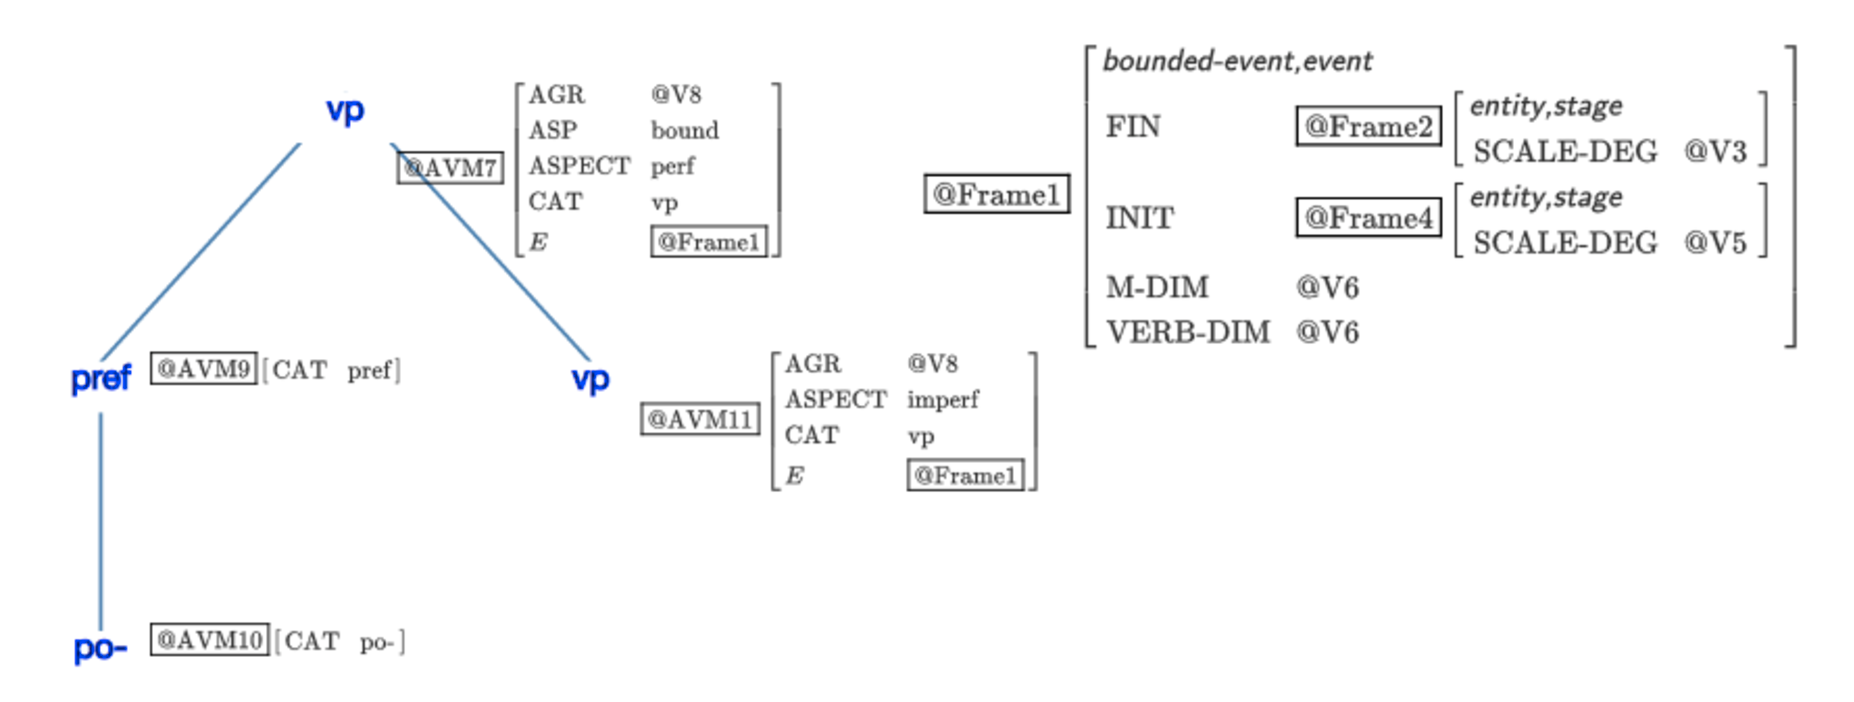
\includegraphics[width=\textwidth]{PoVerb.pdf}
\caption{Result of the compilation of the class \texttt{PoVerb} \label{fig:poverb}}
\end{sidewaysfigure}

%When one contemplates the frame description of the prefix \Prefix{po-} it becomes clear that this prefix rarely can be used in combination with other prefixes or before the attachment of the \isi{secondary imperfective} suffix. If immediately after the attachment of the prefix \Prefix{po-} another prefix is attached, the first step can be just skipped, as it increases the \isi{morphological complexity} and does not influence the resulting semantic representation of the verb. Similar considerations apply if the \Prefix{po-}prefixed verb is to be suffixed with the \isi{imperfective suffix}: normally, the basic \isi{imperfective verbs} would denote the same events as the prefixed and suffixed verb. So even for the presence of some semantic difference, the price of adding two morphemes is too high and such verbs (as \textit{popisyvat'} `to write occasionally, non-seriously') would be used in a restricted number of situations when their meaning is pragmatically enriched. 
%
%If one looks at the situations when the prefix \Prefix{po-} is attached to an already prefixed verb, the picture is also similar: if the last derivation step was \isi{prefixation}, in many cases it has brought at least the semantic information the prefix \Prefix{po-} contains, so further \isi{prefixation} with \Prefix{po-} would be an unnecessary complication. This does not hold for those prefixes that do not overtly add information: e.g., if the verb \textit{zapisat'} `to write down' is suffixed with the suffix \textit{-iva-} in its progressive usage, the resulting verb is defined in terms of being a part of another (bounded) event, but it does not have its own boundaries. The prefix \Prefix{pere-} cannot add such boundaries, as it just copies information, so the verb \textit{perezapisyvat'} `to be rewriting' is imperfective and lacks boundaries, so they will be added when the prefix \Prefix{po-} is attached. Similarly can be explained why the verb \textit{popriotkryt'} `to open very slightly' exists while in other cases an attachment of the prefix \Prefix{po-} to a perfective verb does not seem to be possible (compare with an non-existent verb \textit{*pootkryt'}). In total, the predictions of a semantic-pragmatic analysis in many cases coincide with a syntactic restriction (for \citealt{Tatevosov:13} the prefix \Prefix{po-} is one of the \isi{selectionally limited prefixes}, so it can attach only to \isi{imperfective verbs}) and for some fragments such syntactic restriction may be a fast way of limiting the number of derivation. As we see, however, the analysis proposed here allows for more accurate predictions in complicated cases.
%
%The \isi{distributive} interpretation of the prefix \Prefix{po-} is acquired when the \isi{measure dimension} is the \isi{cardinality scale}. 

Encoding of other prefix usages proceeds in the similar way: the syntactic part does not vary much from prefix to prefix and semantic descriptions can be directly obtained from the frame descriptions I have proposed in Chapter~\ref{Chapter7}. However, there are a couple of difficulties I want to discuss. First let us consider the prefix \Prefix{pere-} in the \isi{repetitive} usage. There are several things that are different compared to the case of the ``\isi{delimitative}'' usage of the prefix \Prefix{po-}. First, the value of the features \textit{aspect} and \textit{bounded} is inherited from the  lower VP and the value of the \textit{limited} feature of the \isi{derivational base} has to be \textit{yes}. Second, at the moment of prefix attachment the central node of the frame shifts: derived VP (node \texttt{?VP} on \figref{code:pere}) is related to the frame \texttt{?X1} whereas the semantics of the \isi{derivational base} is represented by the frame \texttt{?X0} (subframe of \texttt{?X1} on \figref{code:pere}). This realises the solution proposed in the previous chapter. 

\begin{figure}
\begin{lstlisting}[style=xmg]
class PereIterVerb
export ?VP ?VPInt 
declare ?VP ?VPInt ?Pere ?PereLex ?AGR ?X0 ?X1 ?Deg1 ?Deg2 ?Scale ?NounDim
?Aspect ?EventType ?Init ?Fin ?Asp
{
  <syn>{
    node ?VP [cat=vp, agr=?AGR, e=?X1, bounded = ?Asp, limited = yes, 
    				 aspect = ?Aspect];
    node ?Pere [cat=pref];
    node ?PereLex (mark=flex) [cat=pere-];
    node ?VPInt [cat=vp, agr=?AGR, e=?X0, bounded = ?Asp, limited = yes, 
    					  aspect = ?Aspect];
    ?VP -> ?VPInt;
    ?VP -> ?Pere;
    ?Pere -> ?PereLex;
    ?Pere >> ?VPInt
  };
  <frame>{
    ?X1[?EventType,
       m-dim:?Scale[property-scale],
       noun-dim:?NounDim,
       init: ?Init,
       fin: ?Fin,
       prep:?X0[?EventType,
          m-dim:?Scale,
          noun-dim:?NounDim,
          init: ?Init,
          fin: ?Fin]
    ]
  }
}
\end{lstlisting}
\caption{XMG code for the class that describes the repetitive usage of the prefix \Prefix{pere-}\label{code:pere}}
\end{figure}

In order to perform the coercion that is needed when the prefix \Prefix{pere-} is attached to a simplex imperfective verb, a separate step is required. It is realised by the class \texttt{NDimCoercedVerb} (see \figref{xmg:coersion}) that transforms a non-bounded event into a bounded event using the nominal scale.

\begin{figure}
\begin{lstlisting}[style=xmg]
class NDimCoercedVerb
export ?VP ?VPInt
declare ?VP ?AGR ?X0 ?ScMin ?ScMax ?NounDim ?VPInt
{
  <syn>{
    node ?VP [cat=vp, agr=?AGR, e=?X0, bounded = yes, limited = yes, 
    				 aspect = perf];
    node ?VPInt [cat=vp, agr=?AGR, e=?X0, limited = no, aspect = imperf];
    ?VP -> ?VPInt
  };
  <frame>{
    ?X0[bounded-event,
       m-dim: ?NounDim[property-scale & closed-scale,
          min: ?ScMin,
          max: ?ScMax],
       noun-dim:?NounDim,
       init:[stage, 
          scale-deg:?ScMin],
       fin:[stage, 
          scale-deg:?ScMax]
    ]
  }
}
\end{lstlisting}
\caption{XMG code for the class that implements coersion of an unbounded event into a bounded event\label{xmg:coersion}}
\end{figure}

\section{Imperfective suffix}
I use two separate classes to produce two interpretations of \isi{secondary imperfective} verbs: progressive and habitual. For the analysis I propose it is important to distinguish between them when another prefix is attached after the \isi{suffixation}, as these two interpretations have different semantic properties.

The habitual interpretation of the \isi{imperfective suffix}, realised by the code shown on \figref{xmg:habitual}, produces an unlimited event that is a \isi{series of} limited events. The \NOUNDIM of the new event necessarily is of type \textit{cardinality} and does not need to correspond to the respective attribute of the \isi{derivational base}. The \isi{verbal dimension} is copied from the individual event level to the series level. This interpretation of the \isi{imperfective suffix} is also associated with the introduction of the \textit{iteration} type of the event and the respective syntactic feature. The result of the compilation of this class is shown on \figref{fig:iter}.

\begin{figure}
\begin{lstlisting}[style=xmg]
class IterVerb
export ?VP ?VPInt
declare ?VP ?VPInt ?Suf ?Iva ?AGR ?X0 ?X1 ?VDim
{
  <syn>{
    node ?VP [cat=vp, agr=?AGR, e=?X1, bounded = no, limited = no, 
    				  aspect = imperf, iteration = yes];
    node ?Suf [cat=suf];
    node ?Iva (mark=flex) [cat=iva-];
    node ?VPInt [cat=vp, agr=?AGR, e=?X0, limited = yes];
    ?VP -> ?VPInt;
    ?VP -> ?Suf;
    ?Suf -> ?Iva;
    ?VPInt >> ?Suf
  };
  <frame>{
    ?X1[event & iteration,
       segment:?X0[bounded-event,
         noun-dim:[property-scale],
         verb-dim: ?VDim],
       verb-dim: ?VDim,
       noun-dim:[cardinality] 
     ]
  }
}
\end{lstlisting}
\caption{XMG code for the habitual interpretation of the imperfective suffix \label{xmg:habitual}}
\end{figure}

\begin{sidewaysfigure}
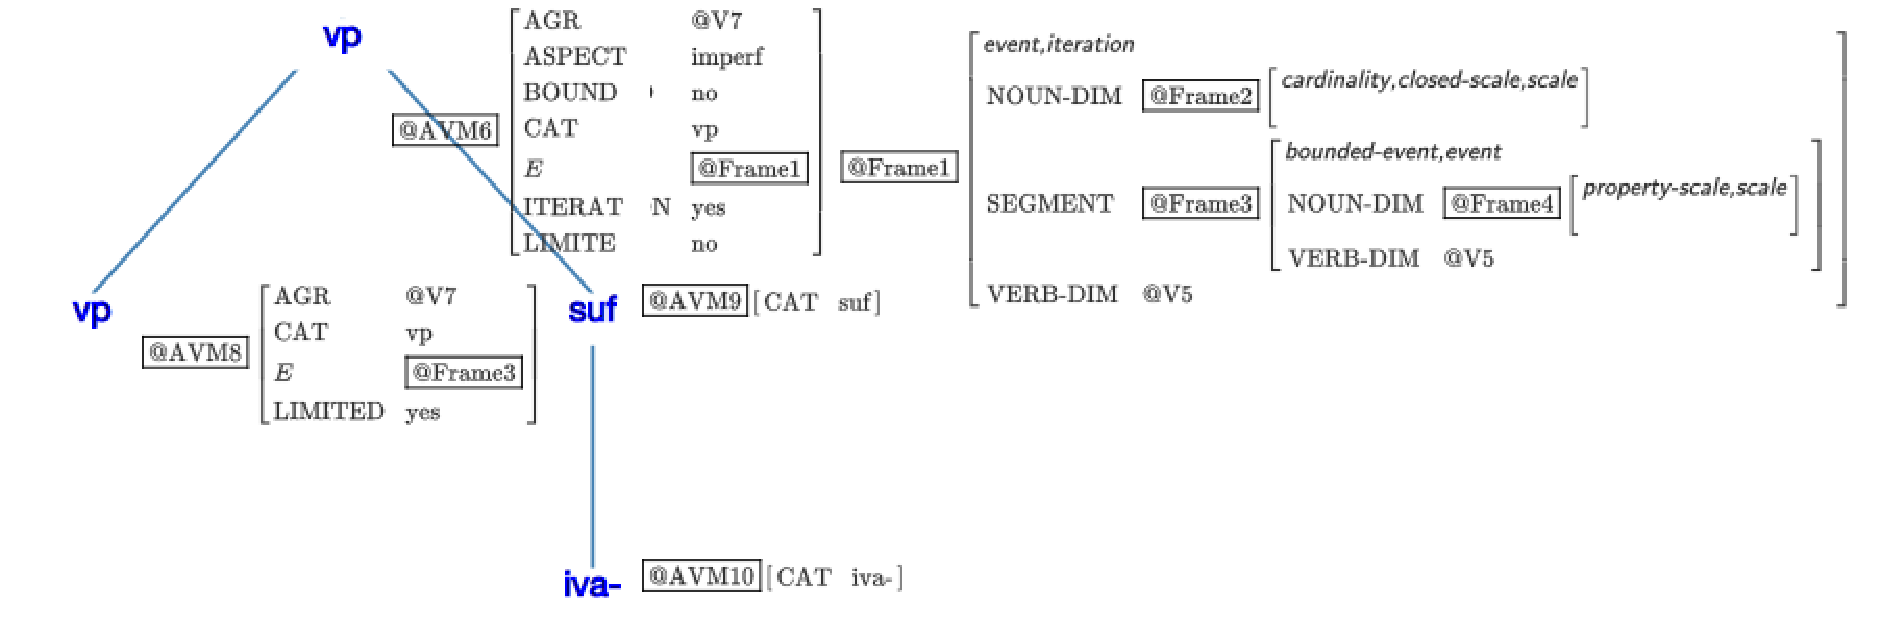
\includegraphics[width=\textwidth]{IterImp.pdf}
\caption{Result of the compilation of the class \texttt{IterVerb}\label{fig:iter}}
\end{sidewaysfigure}

The second interpretation of the \isi{imperfective suffix} is progressive: on the semantic side I represent it as a creation of a new event that is a \PARTOF the event denoted by the \isi{derivational base}. Due to the \PARTOF relation the new event remains limited. On Figures~\ref{graph:pf} and~\ref{graph:ipf} in Chapter~\ref{Chapter1} I have realised \textit{part of} as a relation, as in this case (in contrast to the prefix \Prefix{do-}) it is not functional. As relations are currently not implemented in \isi{XMG}, for the sake of the implementation I use \PARTOF as an attribute when representing the \isi{progressive interpretation} of the \isi{imperfective suffix}.

\section{Assembling the parts}
The last part of the code assembles the verbal phrases from the components described above. As the resource has to be finite, recursion is not allowed in the \isi{XMG} class descriptions.  Due to this restriction, it is not possible to define a single class that would allow an arbitrary number of prefixes to be stacked (by the possibility of attaching a new prefix to the output of the same class). This means that each \isi{prefixation} level has to be described separately. First three classes do the job of assembling verbs with one prefix: the first class (\texttt{OneBasePrefixedVerb}) combines a simplex verb and one of the prefixes; the second class (\texttt{OneCoercedPrefix\-edVerb}) combines a coerced verb with one of the prefixes \Prefix{pere-} (\isi{repetitive} interpretation) and \Prefix{do-}; the last class (\texttt{VerbWithOnePrefix}) assembles under one name the results of the first two classes and all prefixed verbs that are stored in the dictionary. 

\begin{figure}
\begin{lstlisting}[style=xmg]
class TwoPrefixedVerb
export ?VP ?VPInt ?VPBase
declare ?VP ?VPpref ?V ?VSp ?VPInt ?VP ?VPBase
{
  {?VPpref = DoVerb[] | ?VPpref = PereVerb[] | ?VPpref = PereIterVerb[] 
   | ?VPpref = PoVerb[]};
  ?VP = ?VPpref.?VP;
  ?VSp = VerbWithOnePrefix[];
  ?VPInt = ?VSp.?VP;
  ?VPInt = ?VPpref.?VPInt;
  ?VPBase = ?VSp.?VPBase
}
\end{lstlisting}
\caption{XMG code for the verbs with two prefixes \label{xmg:2pref}}
\end{figure}

On the next step (class \texttt{TwoPrefixedVerb}, shown on \figref{xmg:2pref}) the resulting models of the first part are combined again with all available prefix descriptions. This piece of code illustrates how class descriptions are reused: the variable \texttt{?VPpref} gets identified with one of the prefix classes (\texttt{DoVerb}, \texttt{PereVerb}, \texttt{PereIterVerb}, or \texttt{PoVerb}). This is possible only in case all the disjoint classes export the same set of variables. Due to such requirement it is possible to access the exported variables: for example, a \texttt{?VP} variable gets identified with the \texttt{?VP} variable of the \texttt{?VPpref} class (\texttt{?VPpref.?VP}). Similarly the variable \texttt{?VSp} gets identified with a \texttt{VerbWithOnePrefix} class (which, in turn, contains all possible models of verbs with one prefix) and the \texttt{?VPInt} variable is then linked to both the \texttt{?VPInt} node of the \texttt{?VPpref} class and the \texttt{?VP} node of the \texttt{?VSp} class. 

Both types of verbs (with one prefix, \texttt{VerbWithOnePrefix} class, and with two prefixes, \texttt{TwoPrefixedVerb} class) then serve as an input to the class \texttt{SuffVerb}. This class uses the results of \isi{nominal dimension} constructors, as the dimension of the noun can be changed after the attachment of the suffix and it still has to agree with the requirements of the previously attached prefixes. The exported variable \texttt{VPBase} is used to keep track of the attachment point of the semantic representation of the noun. On the syntactic level the noun stays to the right of the verb and will be always attached higher than all the verbal morphemes. 

After the suffixed verbs are assembled, the type matching has to be performed. In the current version of \isi{XMG} type copying is performed not via creating a connection between two types (as it is done with attributes), but by copying the value that is there at the moment the operation is performed. As the noun is attached later, the type of the scale it is associated with is not passed to the higher level if the central node of the frame shifts. To ensure correct typing, I have introduced a class \texttt{TypeMatcher} (code shown on \figref{xmg:typemather}) that identifies all types of the measure dimensions between the higher and the embedded frames (\MDIM, \NOUNDIM, \VERBDIM). The class \texttt{SuffTyped} uses the \texttt{TypeMatcher} class together with the \texttt{SuffVerb} class. In sum, as the VP that contains the scalar interpretation of the noun is identified with the lowest VP available, the type matching mechanism allows to pass the types to a higher level. If the central node of the frame was not changed in the course of prefix attachments, variables \texttt{?X1} and \texttt{?X0} refer to the same frame node.

\begin{figure}
\begin{lstlisting}[style=xmg]
class TypeMatcher
export ?VPOut ?VPInt
declare ?VPInt ?X0 ?X1 ?NDimType ?VDimType ?MDim ?VPOut
{
<syn>{
    node ?VPOut [e=?X1];
    node ?VPInt [e=?X0]
    };
  <frame>{
    ?X1[event,
       m-dim: [?MDim],
       noun-dim: [?NDimType],
       verb-dim: [?VDimType]
    ];
    ?X0[event,
       m-dim: [?MDim],
       noun-dim: [?NDimType],
       verb-dim: [?VDimType]
     ]
  }
}
\end{lstlisting}
\caption{XMG code for the operation of type matching \label{xmg:typemather}}
\end{figure}

I allow for one more derivational step in the described fragment: attachment of a prefix after \isi{suffixation}. This is performed by the class \texttt{TwoPrefixedSuffixedVerb} that uses the result of the compilation of the \texttt{SuffTyped} class and all available prefix classes. At this moment all possible verbal models are created. Then the next step of combining those models with various interpretations of the direct object is performed.

This step is done by two classes: \texttt{PrefixedVerbDirObj} and \texttt{PrefixedSuffixedVerbDirObj} that take, respectively, prefixed and prefixed-suffixed verbs, and all available \isi{dimension constructors}. An output of those classes are models of all possible VPs that use all the available scalar interpretations of the direct objects. This output is again combine with the \texttt{TypeMatcher} class to ensure proper type inheritance.

Before discussing the produced output I would like to note that the architecture of the program is such that as soon as there is a TAG parser that is compatible with frame semantic representation, \isi{lexical anchors} can be removed and the rest of the code would produce unanchored trees with prefixed verbs and appropriate dimension constraints on the argument slot.

%\section{Dimension constructors}
%For the piece I present I need two \isi{dimension constructors}: one referring to the length of the story and another to the cardinality of the set of stories. Both constructors are based on the attributes that are present in the object description: e.g., if there is no \textit{length} attribute in the object frame, the maximum value of the \isi{measure dimension} will be undefined. This is controlled by selecting only appropriate nouns (with a relevant attribute) as those that can undergo the enrichment procedure. Again, as I have to delegate all work to the \isi{metagrammar} compiler, I have to describe such restrictions in the \isi{metagrammar} (see the first line in the class specification), but normally they would be realised as separate \isi{metagrammar} classes and elementary trees for nouns would be accompanied with the information about the possibility of being inserted as \isi{lexical anchors} in such classes.
%
%\begin{figure}
%\begin{lstlisting}[style=xmg]
%%%Creating appropriate dimensions for objects
%
%class NounLength
%export ?N
%declare ?NLength ?X0 ?Length ?N
%{
%  ?NLength=Story[];
%  ?NLength.?Length = ?Length;
%  ?N=?NLength.?N;
%  <syn>{
%    node ?N (mark=coanchor)[cat=n, i=?X0]
%  };
%  <frame>{
%   ?X0[entity,
%        m-dim:[length,
%            min:[zero],
%            max:?Length
%            ]
%      ]
%  }
%}
%
%%% Plural nouns can be interpreted as introducing a \isi{cardinality scale}
%class NounCardinal
%export ?N
%declare ?NCard ?X0 ?Card ?N
%{
%  ?NCard=Story[];
%  ?NCard.?Card = ?Card;
%  ?N=?NCard.?N;
%  <syn>{
%    node ?N (mark=coanchor)[cat=n, num = pl, i=?X0]
%  };
%  <frame>{
%   ?X0[entity,
%        m-dim:[cardinality,
%            min:[zero],
%            max:?Card
%            ]
%      ]
%  }
%}
%\end{lstlisting}
%\caption{Nominal dimension constructors: length and cardinality}
%\end{figure}
%
%After all the constructors are applied, in my implementation they are assembled in one class called \texttt{NDim}. This class creates a VP head and information about \THEME gets included into the newly created event frame. Information about the dimension of the noun is copied to the \NOUNDIM attribute of the event. Note that the case is not specified: this is done in order to account for the possibility of genitive objects and expresses the idea that it is the verb that governs the case assignment and the semantic operation of dimension construction is related but not always governed by the morphological form of the noun. 
%
%\begin{figure}
%\begin{lstlisting}[style=xmg]
%class NDim
%export ?NP ?N ?VP
%declare ?VP ?NP ?X0 ?Theme ?Dim ?Case ?N ?Noun ?Num
%{
%  {?Noun=NounCardinal[] | ?C=NounLength[]};
%  ?N=?Noun.?N;
%  <syn>{
%    node ?NP [cat=np, case=?Case, num = ?Num, i=?Theme];
%    node ?VP [cat=vp, e=?X0];
%    node ?N (mark=coanchor) [cat=n, case = ?Case, num = ?Num, i=?Theme];
%    ?VP >>+ ?NP;
%    ?NP -> ?N
%  }  
%  ;
%  <frame>{
%    ?X0[event,
%          theme:?Theme[entity,
%	          m-dim:?Dim
%          ],
%      noun-dim:?Dim      
%    ]
%  }
%}
%\end{lstlisting}
%\end{figure}

\section{Output}\largerpage
The compilation of the code produces 88 verbal phrases. The full xml of the output is provided in Section~\ref{B:Tat} of Appendix~\ref{AppendixB}. Here I will show and provide a brief analysis of all the obtained models.

The first group of models consists of verbs with one or two prefixes. A total of 16 models is produced (see Table~\ref{table:prefverbs}). Six of these models are models of verbs with one prefix. They all exist, but this is partially due to the selection of the prefixes and the base verb. The upper part of Table~\ref{table:prefverbs} shows these verbs with their English translations and the dimension interpretation of the argument. The last two columns indicate whether the verb exists and if not, whether it will be filtered out by pragmatic module as described in Chapter~\ref{Chapter6}.\largerpage

\begin{table}
\caption{Output of the XMG processing for the class of one- or two-prefixed verbs\label{table:prefverbs}}
\resizebox{\textwidth}{!}{\begin{tabular}{lllll}
\lsptoprule
verb  & semantics & noun  & exists  & blocked by \\
      &           & interpretation & &    pragmatics \\     \midrule
popisat' & to write for some time & length & yes & -- \\ 
dopisat' & to finish writing & length & yes & -- \\ 
perepisat' & to rewrite & length & yes  & --\\ 
zapisat' & to write down & length & yes  & --\\ 
perepisat' & to write all of & cardinal & yes  & --\\ 
popisat' & to write all of & cardinal & yes  & --\\\midrule
dodopisat' & to finish finishing writing & length & yes & -- \\ 
doperepisat' & to finish rewriting & length & yes & -- \\ 
dozapisat' & to finish writing down & length & yes & -- \\ 
peredopisat' & to refinish writing & length & yes & -- \\ 
pereperepisat' & to rewrite again & length & yes  & --\\ 
perezapisat' & to write down again & length & yes & -- \\ 
popopisat' & to write for some time & length & no & yes \\  
perepopisat' & to write all of & cardinal & no & yes \\  
popopisat' & to write all of & cardinal & no & yes \\ 
doperepisat' & to finish writing all of & cardinal & yes & -- \\ 
\lspbottomrule
\end{tabular}}
\end{table}

In the second part of \tabref{table:prefverbs} verbs that contain two prefixes are present. Out of those verbs three must be filtered out for pragmatic reasons since their semantics is equivalent to the semantics of simpler verbs: two variant of the verb \textit{popopisat'} are associated with exactly the same frames as two variants of the verb \textit{popisat'} `to write for some time/to write all of' that can be found in the upper part of the Table~\ref{table:prefverbs}. The third verb that also needs to be discarded is the verb \textit{perepopisat'} that has exactly the same representation as the verb \textit{perepisat'}`to write all of'. 

Note that already at this stage \isi{XMG} reduces 40 possible models (five variants of the first prefix, four variants of the second prefix, and two interpretations of the noun) to only 10 (seven correct and three non-existent) by an appropriate combination of constraints. 

Now let us have a look at the next step: when the verbs from the list above get suffixed with the \isi{imperfective suffix} (in one of two interpretations). The output of this part consists of 23 verbs out of which only two must be filtered out as they are produced on the basis of the verbs that, as we have discussed above, do not exist: \textit{perepopisat'} `to write all of' and \textit{popopisat'} `to write for some time'. It is interesting to note that the second interpretation of the last verb does not get suffixed, so the number of wrong models on the new level does not get multiplied (by the two possible interpretations of the suffix). Instead of the six potential incorrect models just on the basis of the wrong predictions of the previous level we obtain only two. All the verbs produced by this part of the implementation are shown in Table~\ref{table:suffverbs} together with their English translations, interpretation of the \isi{imperfective suffix}, and information about existence.\largerpage

\begin{table}
 \caption{Output of the XMG processing for the class of prefixed and then suffixed verbs\label{table:suffverbs}}
\resizebox{\textwidth}{!}{\begin{tabular}{llll}
\lsptoprule
verb  & semantics & imperfective & exists \\ 
      &      &    interpretation\\\midrule
perepisyvat' & to be writing all of & progressive & yes\\ 
popisyvat' & to be writing for some time habitually & habitual & yes \\ 
dopisyvat' & to be finishing writing & progressive & yes \\ 
dopisyvat' & to finish writing habitually & habitual & yes \\ 
perepisyvat' & to be rewriting & progressive & yes \\ 
perepisyvat' & to rewrite habitually & habitual & yes \\ 
zapisyvat' & to be writing down & progressive & yes \\ 
zapisyvat' & to write down habitually & habitual & yes \\ 
doperepisyvat' & to be finishing writing all of & progressive & yes\\ 
dodopisyvat' & to be finishing writing the final part & progressive & yes \\ 
dodopisyvat' & to finish writing the final part habitually & habitual & yes \\ 
doperepisyvat' & to be finishing rewriting & progressive & yes \\ 
doperepisyvat' & to finish rewriting habitually & habitual & yes \\ 
dozapisyvat' & to be finishing writing down & progressive & yes \\ 
dozapisyvat' & to finish writing down habitually & habitual & yes \\ 
perepopisyvat' & to be writing all of & progressive & no\\ 
peredopisyvat' & to be rewriting the final part & progressive & yes \\ 
peredopisyvat' & to rewrite the final part habitually & habitual & yes \\ 
pereperepisyvat' & to be rewriting again & progressive & yes \\ 
pereperepisyvat' & to rewrite again habitually & habitual & yes \\ 
perezapisyvat' & to be writing down again & progressive & yes \\ 
perezapisyvat' & to write down again habitually & habitual & yes \\ 
popopisyvat' & to be writing for some time habitually & habitual & no\\ 
 \lspbottomrule
 \end{tabular}}
\end{table}

The last group of verbs consists of 49 models that contain at least one prefix attached before the \isi{imperfective suffix} and at least one prefix attached after it. They are shown in Table~\ref{table:prefsuffverbs} together with English translations (not always exact) and the aspect (as here some of the verbs, despite being prefixed on the last derivation step, are imperfective). This part is harder to evaluate as many of the verbs cannot be found on the internet. A possible evaluation method would be to test the unanchored models with various \isi{lexical anchors} against corpus data, but this requires both the parser that supports \isi{frame semantics} (to work efficiently with different verbs) and a large corpus that contains \isi{complex verbs}. I leave these tasks for future research.\largerpage[-1]
 
\begin{longtable}{lll}
\caption{Output of the XMG processing for the class of verbs that are prefixed, then possibly suffixed, and then prefixed again \label{table:prefsuffverbs}}\\
\lsptoprule verb  & semantics & aspect\\ \midrule\endfirsthead%
\midrule verb  & semantics & aspect\\ \midrule\endhead\endfoot\lspbottomrule\endlastfoot
*perepopisyvat' & -- & perfective \\ 
peredopisyvat' & to write the final parts of all of & perfective \\ 
pereperepisyvat' & co copy/rewrite all of & perfective \\ 
perezapisyvat' & to write down all of & perfective \\ 
peredodopisyvat' & to write the very final parts of all of & perfective \\ 
peredoperepisyvat' & to finish rewriting all of & perfective \\ 
peredozapisyvat' & to finish writing down all of & perfective \\ 
pereperedopisyvat' & to rewrite the final parts all of & perfective \\ 
perepereperepisyvat' & co copy/rewrite again all of & perfective \\ 
pereperezapisyvat' & to write down again all of & perfective \\ 
*perepopopisyvat' & \isi{derivational base} does not exist & perfective \\\midrule

*popopisyvat' & to write for some time habitually all of & perfective \\ 
podopisyvat' & to finish writing all of & perfective \\ 
poperepisyvat' & to rewrite all of & perfective \\ 
pozapisyvat' & to write down all of & perfective \\ 
pododopisyvat' & to write the very final parts of all of  & perfective \\ 
podoperepisyvat' & to finish rewriting all of  & perfective \\ 
podozapisyvat' & to finish writing down all of  & perfective \\ 
poperedopisyvat' & to rewrite the final part all of  & perfective \\ 
popereperepisyvat' & co copy/rewrite again all of  & perfective \\ 
poperezapisyvat' & to write down again all of & perfective \\  
*popopopisyvat' & \isi{derivational base} does not exist & perfective\\  \midrule

dodopisyvat' & to finish writing the final part & perfective \\ 
doperepisyvat' & to finish rewriting & perfective \\ 
dozapisyvat' & to finish writing down & perfective \\ 
dododopisyvat' & to finish writing the very final part & perfective \\ 
dodoperepisyvat' & to finish the final part of rewriting   & perfective \\ 
dodozapisyvat' & to finish writing down the final part  & perfective \\ 
doperedopisyvat' & to finish rewriting the final part  & perfective \\ 
dopereperepisyvat' & to finish rewriting again & perfective \\ 
doperezapisyvat' & to finish writing down again & perfective \\  \midrule

peredopisyvat' & to be rewriting the final part & imperf \\ 
pereperepisyvat' & to be rewriting again & imperf\\ 
perezapisyvat' & to be writing down again & imperf\\ 
peredodopisyvat' & to be finishing rewriting the final part & imperf\\ 
peredoperepisyvat' & to be finishing rewriting  again & imperf\\ 
peredozapisyvat' & to be writing down the final part again & imperf \\ 
pereperedopisyvat' & to be rewriting the final part again & imperf \\ 
perepereperepisyvat' & to be rewriting for the forth time & imperf \\ 
pereperezapisyvat' & to be writing down for the third time & imperf \\  \midrule

podopisyvat' & to spend some time finishing writing & perfective \\ 
poperepisyvat' & to spend some time rewriting & perfective \\ 
pozapisyvat' & to spend some time writing down & perfective \\ 
pododopisyvat' & to spend some time finishing the final part & perfective \\ 
podoperepisyvat' & to spend some time finishing rewriting & perfective \\ 
podozapisyvat' & to spend some time finishing writing down & perfective \\ 
poperedopisyvat' & to spend some time rewriting the final part & perfective \\ 
popereperepisyvat' & to spend some time rewriting again & perfective \\ 
poperezapisyvat' & to spend some time writing down again & perfective \\  
\end{longtable}

\pagebreak According to the available data and introspection, out of 49 models four must be discarded. Two of them (\textit{popopopisyvat'} and \textit{perepopopisyvat'}) are formed from the derivational bases that need to be discarded (discussed above). Other two must be discarded by the pragmatic module.

The first of the two verbs, \textit{*perepopisyvat'}, that could have been translated as `to write all of for some time' would be blocked because the interpretation of the prefix \Prefix{pere-} related with the \isi{cardinality scale} is `performing the action completely with each item in the set'. Now, if the interpretation of the prefix \Prefix{po-} does not get strengthened (some time $\rightarrow$ all context-specified time), we obtain a contradiction.  If it does get strengthened (every writing event is maximal with respect to the corresponding member of the set), then the same semantics can be expressed by the simpler verb \textit{perepisat'} `to write all of'. 

The second verb, \textit{*popopisyvat'}, has a similar semantic structure and also could be translated as `to write all of for some time' (see the discussion about the differences between the \isi{distributive} interpretations of the prefixes \Prefix{po-} and \Prefix{pere-} in Chapter~\ref{Chapter5}). This verb refers to the same set of events as the verb \textit{popisat'} with \isi{distributive} interpretation (`to write all of'), although the surface semantic representations of the two verbs are different, so a deeper analysis is needed in this case.

By now we have seen all the models that my implementation produces. Out of 88 models nine should be discarded, but what is harder to evaluate is the recall of the model (fraction of the number of correct models in the output to the number of correct models), as there is no standard that would provide the later number (the total of correct models for the described grammar fragment). I will approach this problem in the next section.

\section{Result evaluation and comparison}
In order to compare the predictions of my model to that of earlier theories, I have implemented the system proposed in \citet{Tatevosov:09} for exactly the same fragment (one verbal stem, one ``lexical'' prefix, five prefix-interpretation pairs, the \isi{imperfective suffix}). For this part I have omitted the lexical entries for direct objects as they do not influence the interpretation of the prefixed verbs. As the approach is syntactic, all restrictions are formulated in syntactic terms and the frame dimension is used to represent the order of attachment of affixes with different semantics. In this implementation, for example, the class for the \isi{distributive} interpretation of the prefix \Prefix{pere-} looks as shown on \figref{xmg:Tat:pere}. The restriction on this prefix attachment is the imperfective aspect of the base verb, which is reflected via a syntactic constraint on the feature \textit{aspect} here.

\begin{figure}
\begin{lstlisting}[style=xmg]
class PereVerb
export ?VP ?VPInt 
declare ?VP ?VPInt ?Pere ?PereLex ?AGR ?X0 ?X1 
{
  <syn>{
    node ?VP [cat=vp, agr=?AGR, e=?X1, aspect = perf];
    node ?Pere [cat=pref];
    node ?PereLex (mark=flex) [cat=pere-];
    node ?VPInt [cat=vp, agr=?AGR, e=?X0, aspect = imperf];
    ?VP -> ?VPInt;
    ?VP -> ?Pere;
    ?Pere -> ?PereLex;
    ?Pere >> ?VPInt
  };
  <frame>{
    ?X1[distributive,
       of: ?X0]
  }
}
\end{lstlisting}
\caption{XMG implementation for the distributive interpretation of the prefix \Prefix{pere-} according to the theory of \citet{Tatevosov:09}\label{xmg:Tat:pere}}
\end{figure}

However, a direct \isi{comparison} of the predictions of the two models is not possible, as \citet{Tatevosov:09} does not offer any theory about the nature of various interpretations of the \isi{imperfective suffix}. Two solutions are available in this situation: either introduce both interpretations of the \isi{imperfective suffix} in the implementation of the theory proposed by \citet{Tatevosov:09} or count those models produced with the implementation of my theory that differ only with respect to the interpretation only once. The second option requires more manual checking, but is more fair with respect to the analysis of \citet{Tatevosov:09}, so I decided to adopt it.

My implementation of the analysis proposed in \citet{Tatevosov:09} produces 81 models for the same fragment. I have done a full analysis of the resulting models and I would like to show the results from verbs with two prefixes and the verbs that are prefixed after the \isi{imperfective suffix} is attached. At the end I will provide the summary with precision, recall, and F-score data for the two models.

%\begin{table}
%\begin{tabular}{p{3.0cm} | p{3cm} | c | c | c}
%verb  & semantics & exists & this model  & Tatevosov 09\\
%perepisyvat' & imperf (to write all of) & yes & + & +\\ \hline
%popisyvat' & imperf (to write for some time) & yes & + & +\\ \hline
%dopisyvat' & imperf (to finish writing) & yes & + & +\\ \hline
%perepisyvat' & imperf (to rewrite) & yes & + & + \\ \hline
%zapisyvat' & imperf (to write down) & yes & + & + \\ \hline
%doperepisyvat' & imperf (to finish writing all of) & yes & + & +\\ \hline
%dodopisyvat' & imperf (to finish writing the final part) & yes & + & + \\ \hline
%dopopisyvat' & imperf (to finish writing for some time) & no & - & + \\ \hline
%doperepisyvat' & imperf (to finish rewriting) & yes & + & + \\ \hline
%dozapisyvat' & imperf (to finish writing down) & yes & + & +\\ \hline
%perepopisyvat' & to be writing all of & no & + & - \\ \hline
%peredopisyvat' & imperf (to rewrite the final part) & yes & + & + \\ \hline
%pereperepisyvat' & imperf (to be rewriting all of) & no & - & + \\ \hline
%pereperepisyvat' & imperf (to rewrite again) & yes & + & + \\ \hline
%perepopisyvat' & imperf (to write for some time again) & no & - & + \\ \hline
%perezapisyvat' & imperf (to write down again) & yes & + & + \\ \hline
%popopisyvat' & to be writing occasionally & no & +  & - \\ \hline
% \hline
% \end{tabular}
%\end{table}
% 
%12 correct (both approaches)
%Tatevosov: 3 wrong
%me: 2 wrong

Table~\ref{table:twopref} shows the full list of verbs produced by two implementations. As we have already discussed above, seven verbs in this list exist and the ``semantic'' implementation produces three models that have to be discarded. The model of the analysis by \citet{Tatevosov:09} produces five verbs that do not exist (under the interpretation associated with them) and three verbs that should be discussed in more detail (marked with question marks in the table).

\begin{table}
\caption{Verbs with two prefixes produced by two implementations \label{table:twopref}}
\begin{tabular}{ll c c c}
\lsptoprule
verb  & semantics & exists & this   & \citeauthor{Tatevosov:09}\\
      &           &        &     account           &  (\citeyear{Tatevosov:09})\\\midrule
dodopisat' & to finish finishing writing & yes & + & + \\ 
doperepisat' & to finish rewriting & yes & + & + \\ 
doperepisat' & to finish writing all of & yes & + & + \\ 
dopopisat' & to finish writing for some time & no & \textminus & + \\ 
dozapisat' & to finish writing down & yes & + & + \\ 
peredopisat' & to refinish writing & yes & + & + \\ 
pereperepisat' & to rewrite all of & no & \textminus & +\\ 
pereperepisat' & to rewrite again & yes & +  & +\\ 
perepopisat' & to write for some time again & no & \textminus & + \\  
perezapisat' & to write down again & yes & + & + \\ 
podopisat' & to finish writing all of & ?? & \textminus & + \\  
poperepisat' & to rewrite all of & ?? & \textminus & + \\  
poperepisat' & to write all of & no & \textminus & + \\  
popopisat' & to write all of for some time & no & \textminus & + \\  
pozapisat' & to rewrite all of & ?? & \textminus & + \\  
popopisat' & to write for some time & no & + & \textminus \\  
perepopisat' & to write all of & no & + & \textminus \\  
popopisat' & to write all of & no & + & \textminus \\ 
\lspbottomrule 
\end{tabular}
\end{table}
%7 exist, predicted by both accounts
%5 false + 3 questionable predicted by Tatevosov 
%3 false predicted by the current approach (to be discarded by the pragmatics module)

These three verbs are verbs that contain the \isi{distributive} prefix \Prefix{po-} stacked over some other prefix (with non-\isi{distributive} interpretation): \textit{podopisat'} `to finish writing all of', \textit{poperepisat'} `to rewrite all of', and  \textit{pozapisat'} `to rewrite all of'. They are, according to the theory proposed in \citet{Tatevosov:09}, possible, but not extensively discussed in the paper (a manuscript by the same author, dedicated to this usage of the prefix and cited among the references, never appeared). I personally do not find them acceptable and \citet[143]{Tatevosov:09} himself marks such verbs as ``interpretable with difficulty''. They could be accommodated in my account if the \isi{distributive} interpretation of the prefix \Prefix{po-} is represented separately and is two-layered, effectively combining in itself the semantics of the \isi{imperfective suffix} (iterative/habitual interpretation) and the current representation of the prefix \Prefix{po-}. The piece of code shown on \figref{xmg:podistr} implements this solution and allows to produce exactly those three verbs (if the class is combined with verbs that are already prefixed once). One would probably want to associate this representation with a higher cost in \isi{comparison} with the initial representation I offer if a subsequent pragmatic module is used.

\begin{figure}
\begin{lstlisting}[style=xmg,basicstyle=\ttfamily\small]
class PoDistrVerb
export ?VP ?VPInt
declare ?VP ?VPInt ?Po ?PoLex ?AGR ?X0 ?X1 ?Init ?Fin ?VDim
{
  <syn>{
    node ?VP [cat=vp, agr=?AGR, e=?X1, limited = yes, bounded = yes, 
    				 aspect = perf, iteration = yes];
    node ?Po [cat=pref];
    node ?PoLex (mark=flex) [cat=po-];
    node ?VPInt [cat=vp, agr=?AGR, e=?X0, bounded = yes];
    ?VP -> ?VPInt;
    ?VP -> ?Po;
    ?Po -> ?PoLex;
    ?Po >> ?VPInt
  };
  <frame>{
    ?X1[bounded-event & iteration,
       m-dim:?VDim[cardinality],
       verb-dim: ?VDim,
       segment:?X0[event,
         m-dim:[property-scale]
       ]
    ]
  }
}
\end{lstlisting}
\caption{XMG code for implementing the `coerced' distributive interpretation of the prefix \Prefix{po-}\label{xmg:podistr}}
\end{figure}

If the three verbs that we have just discussed are considered existent, then the \isi{prefixation} system proposed by \citet{Tatevosov:09} produces five models that must be discarded. In contrast with my proposal, there is no further explanation of why exactly those verbs (two of them are produced by the same rule that forms the three verbs we have just discussed) would be problematic.

Among the verbs with one or two prefixes and an \isi{imperfective suffix} added at the last step of the derivation the number of errors stays close (two versus three), although again constructed but not existent verbs are distinct in two approaches. Both implementations have full recall with respect to this part and the part we have discussed before.

The \isi{comparison} becomes more interesting when  we consider the most \isi{complex verbs} created by the two implementations. The number of models produced here is close: 45 models according to the analysis by \citet{Tatevosov:09} and 49 models in the implementation of my analysis. The overlap of these sets constitutes, however, only 27 models. The first thing to note is that the group of verbs that are marked as imperfective in Table~\ref{table:prefsuffverbs} cannot be (and is not) produced in the system proposed by \citet{Tatevosov:09}. One may ask whether they should be produced at all: an attentive reader probably noticed that both Table~\ref{table:suffverbs} and Table~\ref{table:prefsuffverbs} contain, for example, the imperfective verb \textit{perezapisyvat'} `to be writing down again'. The structure of the two verbs, however, is different: in one case the \isi{imperfective suffix} is attached as the last step of the derivation and in the other case it happens before the \isi{repetitive} \Prefix{pere-} is attached. On the semantic side this is reflected in what ends up to constitute the preparatory stage of the event: once it is the whole completed event of the same type, and in the second case it is another ongoing/partial event. Another difference is that only in the first structure the habitual interpretation of the suffix is possible. 

The second group of \isi{complex verbs} that is not produced by the implementation of the analysis offered in \citealt{Tatevosov:09} is formed by the verbs with the outermost prefix \Prefix{do-}. They follow the pattern we have extensively discussed in Chapter~\ref{Chapter2}.

Among the rest of the models produced by the second implementation are such verbs as \textit{pereperepopisyvat'} with a semantic structure of a \isi{distributive} interpretation over imperfective of the \isi{repetition} of a delimited event. Such semantic structures are hardly conceivable and the corresponding verbs do not exist.\footnote{This judgement is mostly based on introspection and personal communication with other native speakers, as any such verb would be rare and the absence of data on the Internet is not a reliable indicator of the non-existence. I plan to conduct additional experiments in future to get statistically reliable evidence about the existence of such \isi{complex verbs}.}

%\begin{tabular}{p{3cm} | p{6cm} | p{2cm}} 
%verb  & semantics & aspect\\ \hline
%+*perepopisyvat' & -- & perfective \\ \hline
%+peredopisyvat' & to write the final parts of all of & perfective \\ \hline
%pereperepisyvat' & for all: imperf (write all of) & Tatevosov\\
%+pereperepisyvat' & co copy/rewrite all of & perfective \\ \hline
%+perezapisyvat' & to write down all of & perfective \\ \hline
%+peredodopisyvat' & to write the very final parts of all of & perfective \\ \hline
%+peredoperepisyvat' & to finish rewriting all of & perfective \\ \hline
%peredoperepisyvat' & for all: imperf (finish rewriting all of) & Tatevosov \\ \hline
%peredopopisyvat' & distr (imp (compr (delim))) & Tatevosov \\ \hline
%+peredozapisyvat' & to finish writing down all of & perfective \\ \hline
%+pereperedopisyvat' & to rewrite the final parts all of & perfective \\ \hline
%perepereperepisyvat' & co copy/rewrite again all of & perfective \\ \hline
%perepereperepisyvat' & distr (imp (rep (distr))) & Tatevosov \\ \hline
%pereperepopisyvat' & distr (imp (rep (delim))) & Tatevosov \\ \hline
%+pereperezapisyvat' & to write down again all of & perfective \\ \hline
%*perepopopisyvat' & \isi{derivational base} does not exist & perfective \\ \hline  \hline
%
%
%+*popopisyvat' & distr (imp (delim)) & perfective \\ \hline
%+podopisyvat' & to finish writing all of & perfective \\ \hline
%+poperepisyvat' & to rewrite all of & perfective \\ \hline
%poperepisyvat' & distr (imp (distr)) & Tatevosov \\ \hline
%+pozapisyvat' & to write down all of & perfective \\ \hline
%+pododopisyvat' & to write the very final parts of all of  & perfective \\ \hline
%+podoperepisyvat' & to finish rewriting all of  & perfective \\ \hline
%podoperepisyvat' & distr (imp (compl (distr))) & Tatevosov \\ \hline
%podopopisyvat' & distr (imp (compl (delim))) & Tatevosov \\ \hline
%+podozapisyvat' & to finish writing down all of  & perfective \\ \hline
%+poperedopisyvat' & to rewrite the final part all of  & perfective \\ \hline
%+popereperepisyvat' & co copy/rewrite again all of  & perfective \\ \hline
%popereperepisyvat' & distr (imp (rep (distr))) & Tatevosov \\ \hline
%+poperezapisyvat' & to write down again all of & perfective \\ \hline
%poperepopisyvat' & distr (imp (rep (delim))) & Tatevosov \\ \hline
%*popopopisyvat' & \isi{derivational base} does not exist & perfective\\ \hline
%
%dodopisyvat' & to finish writing the final part & perfective \\ \hline
%doperepisyvat' & to finish rewriting & perfective \\ \hline
%dozapisyvat' & to finish writing down & perfective \\ \hline
%dododopisyvat' & to finish writing the very final part & perfective \\ \hline
%dodoperepisyvat' & to finish the final part of rewriting   & perfective \\ \hline
%dodozapisyvat' & to finish writing down the final part  & perfective \\ \hline
%doperedopisyvat' & to finish rewriting the final part  & perfective \\ \hline
%dopereperepisyvat' & co finish rewriting again & perfective \\ \hline
%doperezapisyvat' & to finish writing down again & perfective \\ \hline \hline
%
%peredopisyvat' & to be rewriting  the final part & imperfective \\ \hline
%pereperepisyvat' & to be rewriting again & imperfective\\ \hline
%perezapisyvat' & to be writing down again & imperfective\\ \hline
%peredoperepisyvat' & to be finishing rewriting  again & imperfective\\ \hline
%peredozapisyvat' & to be writing down the final part again & imperfective \\ \hline
%pereperedopisyvat' & to be rewriting the final part again & imperfective \\ \hline
%perepereperepisyvat' & to be rewriting for the forth time & imperfective \\ \hline
%pereperezapisyvat' & to be writing down for the third time & imperfective \\ \hline \hline
%
%+podopisyvat' & to spend some time finishing writing & perfective \\ \hline
%+poperepisyvat' & to spend some time rewriting & perfective \\ \hline
%poperepisyvat' & to spend some time writing all of & Tatevosov \\ \hline
%popopisyvat' & to spend some time writing for some time & Tatevosov \\ \hline
%+pozapisyvat' & to spend some time writing down & perfective \\ \hline
%+pododopisyvat' & to spend some time finishing the final part & perfective \\ \hline
%+podoperepisyvat' & to spend some time finishing rewriting & perfective \\ \hline
%podoperepisyvat' & delim (imp (comp (distr))) & Tatevosov \\ \hline
%podopopisyvat' & delim (imp (comp (delim))) & Tatevosov \\ \hline
%+podozapisyvat' & to spend some time finishing writing down & perfective \\ \hline
%+poperedopisyvat' & to spend some time rewriting the final part & perfective \\ \hline
%+popereperepisyvat' & to spend some time rewriting again & perfective \\ \hline
%popereperepisyvat' & delim (imp (rep (distr))) & Tatevosov \\ \hline
%poperepopisyvat' & delim (imp (rep (delim))) & Tatevosov \\ \hline
%+poperezapisyvat' & to spend some time writing down/copying again & perfective \\ \hline
%\end{tabular}
%\caption{Output of the XMG processing for the class of verbs that are prefixed, then possibly suffixed, and then prefixed again {table:prefsuffverbs}}
%\end{table}

%6+ 7 +3 + 12 + 27 + 18 = 28 + 28 + = 73
%6+10+12+27 = 28+27 = 55
%5+3 +18
%-3 +2+4+3
%So out of 45 models produced for the prefixed, suffixed, and then prefixed again verbs by the implementation of the analysis proposed in \citet{Tatevosov:09} I think that 27 exist, 18 do not, and 18 are missed. 
%
%
%Tatevosov: total 121. Me: total 88. -9 = 79
%Overlap: 51 correct models + 2 incorrect both approaches + 18 correct my approach  + 7 wrong my approach
%+ 25 wrong Tatevosov + 3 questionable Tatevosov + 40 incorrect
%51 - 3 - 67
%51 + 17 + 3 = 71
%+9

To quantify precision and recall, I decided to do the following:
\begin{itemize}
\item count 79 models instead of 88 for my analysis by removing such models that differ only with respect to the interpretation of the \isi{secondary imperfective};
\item count the models for the existence of which I argue in Chapter~\ref{Chapter2} as correct (\isi{imperfective verbs} formed when the last affix attached is the \isi{repetitive} \Prefix{pere-} and perfective \Prefix{do-}prefixed verbs)
\item calculate all measures two times: once counting three questionable verbs as incorrect (Table~\ref{table:precision}) and once counting them as correct (Table~\ref{table:precision2});
\item on pair with the previous decision I will use two versions of the implementation of my analysis: the original one and one that uses the update shown in \figref{xmg:podistr}.
\end{itemize}
 
Based on this, I obtain the following numbers: for the implemented fragment there are 70 or 73 correct models\footnote{I have manually checked the possibilities using the assumption that there can be no existing complex verb derived from a non-existing verb. The calculation of the recall is thus based on this assumption.}. Out of these models, the implementation of the analysis provided in \citet{Tatevosov:09} produces, respectively, 52 or 55, and the total number of models output is 81. The original implementation of my analysis produces 70 correct models and the total number of models (after the duplicates among \isi{imperfective verbs} are removed) is 79. The updated version produces 70 and 73 of the correct models, respectively, and the total number of models in this case is 82. The precision (fraction of correct models out to all produced models), recall (fraction of correct models in the output to all correct models), and F-measures ($2*(precision*recall)/(precision+recall)$) are provided in Table~\ref{table:precision} for the first version of calculation (three questionable models excluded) and in Table~\ref{table:precision2} for the second version.
 
 \begin{table}
 \caption{Precision, recall and F-measure for different implementations (three questionable verbs excluded) \label{table:precision}}
 \begin{tabular}{l *{3}{S[table-format=1.3]}}
 \lsptoprule
 analysis & {precision} & {recall} & {F-measure}\\ \midrule
 current analysis original & 0.886 & 1 &  0.94\\
 \citet{Tatevosov:09} & 0.642 & 0.743 & 0.689\\
 current analysis modified &  0.854 & 1 & 0.921\\ \lspbottomrule
 \end{tabular}
 \end{table}
 
  \begin{table}
 \caption{Precision, recall and F-measure for different implementations (three questionable verbs included) \label{table:precision2}}
  \centering
 \begin{tabular}{l  *{3}{S[table-format=1.3]}}
 \lsptoprule
 analysis & {precision} & {recall} & {F-measure}\\ \midrule
 current analysis original & 0.886 & 0.959 &  0.921\\
 \citet{Tatevosov:09} & 0.679 & 0.753 & 0.714\\
 current analysis modified &  0.89 & 1 & 0.942\\
 \lspbottomrule
 \end{tabular}
 \end{table}
 
The numbers in the tables show that despite the close number of the models in the output there is a significant difference in precision and recall between the implementation of the analysis proposed here and that of the analysis from \citet{Tatevosov:09}. In addition I have shown that my analysis can easily be adapted in case of different acceptability judgements to obtain the full recall. I also offer pragmatic reasoning to exclude the models that do not belong to the set of correct ones. Besides that the output of the analysis contains fully spelled-out semantic representations that are obtained \isi{compositionally} and the semantics of the prefix in a given position is derived and not stipulated.
 % XMG
% Chapter 9

\chapter{Conclusions, remarks and further questions} % Write in your own chapter title
\label{Chapter9}
%\lhead{Chapter 8. \emph{Conclusions, remarks and further questions}} % Write in your own chapter title to set the page header

In this work I have explored the Russian verbal prefixation system and proposed a complex account that models it. In Chapter~\ref{Chapter2} I have presented new data that did not receive an appropriate analysis within the earlier accounts of Russian prefixation. I have also developed a method of collecting data that prevents any decisions that may be biased by the theory one proposes. This method was used throughout the entire work to ensure careful data representation.

After considering the data I have discussed the commonly assumed distinction between lexical and superlexical prefixes in Chapter~\ref{Chapter4}. I have shown that despite the clear differences between the properties of particular prefixes the proposal of the strict distinction between the classes has to be rejected together with the possibility to restrict prefix stacking due to different positions of various prefixes. The division into prefix classes is then substituted with a scale. One end of this scale is occupied by those prefixes that do not have a predictable semantic contribution, can never stack on top of other prefixes, and change the argument structure of the verb. On the other end of the scale are located those prefixes that have a transparent semantics, can stack freely and do not change the argument structure of the verb. Other prefixes are located in between these extremes without clear class borders. On this basis I have decided to abandon the hypothesis of different structural positions of various prefixes and develop a semantic account that would have at least the same predictive power with respect to possible affix combinations and also explains the data presented in Chapter~\ref{Chapter2}.

In Chapter~\ref{Chapter5}, I went through the first step towards a semantic account of verbal prefixation in Russian: I provided an informal analysis of the semantic and combinatorial properties of five prefixes (\textit{za-, na-, po-, pere-} and \Prefix{do-}) as well as a brief discussion of the (simplified) treatment of the imperfective suffix that I assume. I then continued with the exploration of the pragmatic properties of individual prefixes and of the competition between various prefixed verbs derived from the same base in Chapter~\ref{Chapter6}. I have shown that there is not enough evidence to assume the presuppositional account of the prefixes \Prefix{do-} and \Prefix{pere-} and concluded that the inferences associated with their usage should be treated as entailments and implicatures. In the second part of the chapter I have outlined a preliminary version of the pragmatic competition between prefixed verbs. I have shown some examples of how the interpretation of a prefixed verb can be derived using underspecified semantics and basic pragmatic principles. 

Following the theoretical part,  in Chapter~\ref{Chapter7} I have provided a frame semantic analysis of the five prefixes which I have explored in this work. I have introduced the formalism, provided frame representations of various prefixes and shown how these frames combine with verbal frames, frames for the direct object, measure phrases, and special dimension constructors. To evaluate the predictions of the analysis I have implemented it for a small language fragment using the metagrammar description formalism (XMG). I have provided the details of the implementation and discussed the difficulties related to it in Chapter~\ref{Chapter8}. I have also implemented the proposal of \citet{Tatevosov:09} and compared the output of the two proposals with respect to the predictive power of available affix combinations for a given verb. 

In sum, I have provided and partially implemented an account that predicts the possibility of prefix attachment (for five prefixes) and in case of a positive answer also the semantics, aspect, and semantic and syntactic restrictions on the arguments of the derived verb. 

On the other hand, I have raised a number of questions that could not be answered in course of this work and are worth further investigation. These are, for example, questions about the unexpected behaviour of loaned biaspectual verbs when they are prefixed with \Prefix{do-} or \Prefix{pod-} and about the status of loaned prefixes, such as \Prefix{dis-} or \Prefix{re-}. I also have not examined the behaviour of the imperfective suffix in detail and instead used a simplification that has to be replaced with a more thorough description in the future. 

Another research direction that I aim to address in my future work is the development of the pragmatic part. I hope to implement the proposal concerning the competition of various prefixed verbs using the Rational Speech Act framework. In parallel, I would like to run the experiments to obtain probabilistic predictions for various interpretations of the prefixed verbs.  Of particular interest are cases where, according to my analysis, a particular interpretation is part of the semantics of the verb, but is blocked for pragmatic reasons. I then plan to compare the quantitative output of the implemented system with experimental results that would allow to test the whole theory in an objective way.

The implementation of the proposal I have done so far also needs to be extended. This would be possible as soon as the relevant tools are available (most important of which is a parser that would work with TAG and frame representations) and the contribution of other prefixes is represented in terms of frames. A large-scale implementation would allow to create the derivational graph, as proposed in Chapter~\ref{Chapter2}, that would open the way for further research and testing in the domain of Russian complex verbs. 
 % Conclusion

\appendix
\chapter{Frame representations}\label{AppendixA}
\section{Constraints}\label{app:constraints}
\ex.\label{app:const:proper}\textit{proper-scale} $\und$ \textit{measure-of-change} $\rightarrow \bot$

\ex.\label{app:const:temp:amount}\textit{amount} $\und$ \textit{temperature} $\rightarrow \bot$

\ex.\label{app:const:card}\textit{event $\und$ cardinality $\rightarrow$ iteration}

\ex.\label{app:constr:duration}\textit{bounded-event} $\und$ \DURATION .$\top$ $\rightarrow$ (\MDIM .\textit{measure-of-change} $\und$ time) $\und$  \MDIM .\MIN = 0 $\und$ \MDIM .\MAX $\triangleq$ \DURATION .\VAL

\ex.\label{app:rule:minmaxevent}\a. \MIN .$\top$ $\und$ \INIT .$\top$ $\rightarrow$ \INIT .\POS $\triangleq$ \MIN
\b. \MAX .$\top$ $\und$ \FIN .$\top$ $\rightarrow$ \FIN .\POS $\triangleq$ \MAX

\section{Prefixes}\label{app:pref}

\begin{figure}[H]
\centering
\begin{forest}
[VP\textsuperscript{[E=\textbf{f}]}
  [Pref [za-]]
  [VP\textsuperscript{[E=\textbf{e}]}]
]
\end{forest}
\begin{tabular}[t]{ll}
\begin{tabular}[t]{l}
\avm{
\btag{f} [\type*{transition}
      \POST & [\type*{event}
         \MDIM & [\type*{proper-scale}
            \MIN & deg ] 
     ]
   ]
}
\end{tabular}
\begin{footnotesize}
\begin{tabular}[t]{l}
$\tuple{\btag{f}\BC\POST,\btag{e}}\D\type{esegm-of}$\\[1ex]
$\tuple{\btag{f}\BC\POST\C\MDIM,\btag{e}\BC\MDIM}\D\type{segm-of}$\\
\end{tabular}
\end{footnotesize}
\\\\
\begin{tabular}[t]{l}
\avm{
\btag{e} [\type*{event}
	 \VERBDIM & \1\\
     \MDIM & \1 [\type*{proper-scale}]
   ]
}
\hfill
\end{tabular}
\end{tabular}
\hfill
\caption{Representation of the contribution of the prefix \textit{za-}}
\label{app:za.frame.semantics}
\end{figure}

\begin{figure}[H]
\begin{minipage}{0.4\textwidth}
\avm{
\btag{e} [\type*{bounded-event}
	   \NOUNDIM & \3\\       
	   \VERBDIM & \3\\
       \MDIM & \3[\type*{scale}
			\MIN & \1 \\	  
			\THRESHOLD & \2
       ] \\
       \INIT & [\type*{stage}
     		\POS & \1]\\
      \FIN & [\type*{stage} 
  		 	\POS & \4 ]\\
   ]
}\\
\vspace{1cm}
\centering
\svar{2} $\leq$ \svar{4}
\end{minipage}
\hfill
\begin{minipage}{0.4\textwidth}
\begin{forest}
[VP\textsuperscript{E=\textbf{e}}
  [Pref [na-]]
  [VP\textsuperscript{[E=\textbf{e}]}]
]
\end{forest}
\end{minipage}
\caption{Representation of the contribution of the prefix \textit{na-}\label{app:na}}
\end{figure}

\begin{figure}[H]
% \begin{minipage}{0.4\textwidth}
\avm{
\btag{e} [\type*{bounded-event}
   	   \VERBDIM & \1\\
       \MDIM & \1 [\type*{scale}] \\
       \INIT & [\type*{stage}
     		\POS & \2]\\
       \FIN & [\type*{stage} 
  		 	\POS & \3 ]\\
   ]
}\hfill%
% \end{minipage}
% \begin{minipage}{0.55\textwidth}
\avm{
\btag{e}  [\type*{bounded-event}
   \NOUNDIM & \3\\
    \MDIM & \3 [
       \type*{closed-scale $\und$ proper-scale}
       \MIN & \1\\
       \MAX & \2]\\
    \INIT & [\type*{stage}
       \POS & \1 ]\\
     \FIN & [\type*{stage}
       \POS & \2 ]
  ]
}
% \end{minipage}
%% Add requirement that if m-dim = path, path-start = init
\caption{Frame representations of the prefix \textit{po-} (left) and of of the prefix \textit{pere-} for the closed scale case (right) \label{app:po:delim}}
\end{figure}

\begin{figure}[H]\small
\begin{minipage}{0.5\textwidth}
\avm{
\btag{e} [\type*{bounded-event}
  	\NOUNDIM & \4\\
    \MDIM & \4 [
       \type*{proper-scale $\und$}\type*{one-marked-point}
       \MARKED & \2 ]\\
    \INIT & [\type*{stage}
       \POS & \1 ]\\
     \FIN & [\type*{stage}
       \POS & \3 ]\\
  ]
}\\
\centering
\svar{1} $<$ \svar{2} $<$ \svar{3}
 \end{minipage}\hfill%
 \begin{minipage}{0.45\textwidth}
\avm{
\btag{f}  [\type*{bounded-event}
     \MDIM & \3 [\type*{property-scale} ]\\
     \NOUNDIM & \4\\
     \INIT &  \1\\
     \FIN &  \2 \\
     \MANN & \5\\
     \PREP & \btag{e} [\type*{event}
  	 	\THEME & \6\\
        \MDIM & \3\\
    	\NOUNDIM & \4\\
    	\INIT &  \1\\
     	\FIN &  \2 \\
     	\MANN & \5
     ]
  ]
 }
 \end{minipage}
\caption{Frame representation of the prefix \textit{pere-}: case of a one marked point scale on the left and case of a property scale on the right \label{app:pere:iter}}
\end{figure}

\begin{figure}[H]\small
\begin{minipage}{0.45\textwidth}
\avm{
\btag{f} [\type*{bounded-event}
   		\MANN & \4\\
   		\ACTOR & \5\\
  	 	\THEME & \9\\
        \MDIM & [ \type*{closed-scale}\type*{$\und$ property-scale}
			\MIN & \2\\
			\MAX & \1						
        ]\\
    	\INIT & [\type*{stage}
    		\POS &  \3]\\
     	\FIN &  [\type*{stage}
    		\POS &  \1]\\
     	\PARTOF & \btag{e}\\
       \NOUNDIM & [\7]\\
       \VERBDIM & [\8]
    ]
 }
 \end{minipage}\hfill%
 \begin{minipage}{0.45\textwidth}
\avm{
\btag{e} [\type*{bounded-event}
   		\MANN & \4\\
   		\ACTOR & \6\\
  	 	\THEME & \9\\
        \MDIM & [ \type*{closed-scale}\type*{$\und$ property-scale}
			\MAX & \1						
        ]\\
    	\INIT &  [\type*{stage}
    		\POS &  \2]\\
     	\FIN &  [\type*{stage}
    		\POS &  \1]\\
       \NOUNDIM & [\7]\\
       \VERBDIM & [\8]
    ]
 }\\
 \vspace{0.5em}
 \centering
$\tuple{\btag{f}\BC\MDIM,\btag{e}\BC\MDIM}\D\type{segm-of}$\\[1ex]
\end{minipage}
\caption{Frame representation of the prefix \textit{do-} \label{app:do}}
\end{figure}

\pagebreak

\section{Verbs}\label{app:verbs}
\begin{figure}[H]
% \begin{minipage}{0.32\textwidth}
\avm{
\btag{e} [\type*{transloc}
	   \MANN & [\type*{run}]\\
       \ACTOR & \1\\
	   \TRACE & \2
]
}\hfill%
% \end{minipage}
% \begin{minipage}{0.33\textwidth}
\avm{
\btag{e} [\type*{transloc}
	   \MANN & [\type*{fly}]\\
       \ACTOR & \1\\
	   \TRACE & [\type*{trace}]\\
	   \PATH & \2 [\type*{path}]\\
	   \VERBDIM & \2\\
	   \MDIM & \2
]
}\hfill%
% \end{minipage}
% \begin{minipage}{0.3\textwidth}
\avm{
\btag{e} [\type*{transloc}
	   \MANN & [\type*{run}]\\
       \ACTOR & \1\\
	   \TRACE & [\type*{trace}]\\
	   \PATH & \2 [\type*{path}]\\
	   \VERBDIM & \2\\
	   \MDIM & \2
]
}%
% \end{minipage}
\caption{Verbs \textit{begat'}$^{\INDET}$ `to run' (left), \textit{letat'}$^{\DET}$ `to fly' (center), and \textit{be\v{z}at'}$^{\DET}$ `to run' (right)}
\end{figure}

\begin{figure}[H]\small
% \begin{minipage}{0.48\textwidth}
\avm{
 \btag{e} [\type*{state}
  		\STATE & [\type*{be\_seen}]\\
  		\THEME & \1 [
  			\COLOR & [\type*{yellow}]\\
  		]\\
  		\VERBDIM & \btag{e}
  ]
}\hfill%
% \end{minipage}
% \begin{minipage}{0.47\textwidth}
\avm{
\btag{e} [\type*{change-of-state}
  \VERBDIM & \2 [\type*{property-scale}\type*{$\und$ yellow} 
  	\MIN & \3\\
  	\MAX & \4  
  ]\\
  \MDIM & \2\\
  \THEME & \1
]
}%
% \end{minipage}
\caption{Two interpretations of the verb \textit{\v{z}eltet'} `to be yellow and be seen/to become yellow' \label{app:zeltet}}
\end{figure}

\begin{figure}[H]\small
% \begin{minipage}{0.3\textwidth}
\avm{
\btag{e} [\type*{event $\und$iteration}
    \MANN & [\type*{burst}]\\
    \ACTOR & \1\\
    \THEME & \2\\
    \VERBDIM & \btag{e}
  ]
}\hfill%
% \end{minipage}
% \begin{minipage}{0.35\textwidth}
\avm{
\btag{e} [\type*{process}
	   \MANN & [\type*{cook}]\\
       \ACTOR & \2\\
	   \THEME & [\type*{food}
	   		\AMOUNT & \1 ]
]
}\hfill%
% \end{minipage}
% \begin{minipage}{0.3\textwidth}
\avm{
\btag{e} [\type*{process}
    \MANN & [\type*{live}]\\
    \ACTOR & \1\\
    \VERBDIM & \btag{e}\\
    \MDIM & \btag{e}
  ]
}%
% \end{minipage}
\caption{Verbs \textit{lopat'} `to burst' (left), \textit{varit'} `to cook' (center), and \textit{\v{z}it'} `to live' (right) \label{app:frame:lopat}}
\end{figure}

\begin{figure}[H]
% \begin{minipage}{0.48\textwidth}
\avm{
\btag{e} [\type*{change-of-state}
	   \MANN & [\type*{heat}]\\
       \ACTOR & \1\\
	   \THEME & \2\\
	   \VERBDIM & \3 [\type*{temperature}]\\
	   \MDIM & \3
]
}\hfill%
% \end{minipage}
% \begin{minipage}{0.47\textwidth}
\avm{
  \btag{e} [\type*{process $\und$ closed-scale}
    \MANN & [\type*{spend-time $\und$ winter}]\\
    \ACTOR & \1\\
    \VERBDIM & \btag{e}\\
    \MDIM & \btag{e}\\
    \MIN &  [\type*{winter-start}]\\
    \MAX &  [\type*{winter-end}]\\
  ]
}%
% \end{minipage}
\caption{Verbs \textit{gret'} `to heat' (left) and  \textit{zimovat'} `to spend winter time' (right) \label{app:live}}
\end{figure}


\section{Nouns}\label{app:nouns}
\begin{figure}[H]\small
% \begin{minipage}{0.6\textwidth}
\avm{
\btag{f} [\type*{soup}
	   \AMOUNT & [\type*{amount}
	   		\VAL & \1\\
	   		\MUNIT & ml ] \\
       \TEMP & [\type*{temperature}
	   		\VAL & \2\\
	   		\MUNIT & °C ] \\
       \KIND & [\type*{soup-kind}]\\
       \TASTE & [\type*{taste}]\\
       \AMOUNTDIM & [\type*{amount $\und$}\type*{measure-of-change}
       		\MIN & 0\\
       		\MAX & \1
       	]\\
       	\TEMPDIM & [\type*{temperature $\und$}\type*{proper-scale}
       		\MIN & \2\\ 
       		\MAX & 100
       	]
]
}\hfill%
% \end{minipage}
% \begin{minipage}{0.35\textwidth}
\avm{
\btag{g} [\type*{match}
	   \DURATION & \1\\
	   \GAME & [\type*{game}]\\
	   \PLAYERS & [\type*{entity}
	   		\CARD & \2
	   ] 
]
}%
% \end{minipage}
\caption{Nouns \textit{sup} `soup' (left) and \textit{partija} `match' (right)}
\end{figure}

\begin{figure}[H]
% \begin{minipage}{0.3\textwidth}
\avm{
\btag{f} [\type*{road}
	   \WIDTH & \1\\
	   \LOC & \2\\
	   \EDGE & \3
]
}\hfill%
% \end{minipage}
% \begin{minipage}{0.3\textwidth}
\avm{
\btag{f} [\type*{hurricane}
	   \TIME & \1\\
	   \LOC & \2\\
	   \NAME & \3
]
}\hfill%
% \end{minipage}
% \begin{minipage}{0.35\textwidth}
\avm{
\btag{f} [\type*{balloon}
	   \CARD & [\type*{cardinality}
       		\POS & \1
       	]\\
       \SIZE & \2\\
       \COLOR & \3
]
}%
% \end{minipage}
\caption{Nouns \textit{doroga} `road' (left), \textit{uragan} `hurricane' (center), and \textit{\v{s}ar} `balloon' (right) \label{app:road}}
\end{figure}

\section{Measure phrases}\label{app:measure}
\begin{figure}[H]
\begin{tabular}[b]{c}
\begin{forest}
[NumP\textsuperscript{[I=\textbf{f}]}
[Num] [N]
]
\end{forest}\\
\avm{
\btag{f} [\type*{length}
  		\VAL & 2\\
  		\MUNIT & hour  
  ]
}
\end{tabular}
\hspace{2cm}
\begin{tabular}[b]{c}
% % 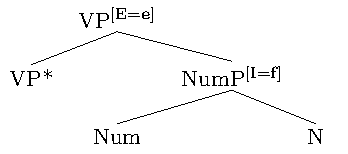
\includegraphics[scale=1]{VNumP.pdf}\\
\begin{forest}
[VP\textsuperscript{[E=\textbf{e}]}
  [VP*]
  [NumP\textsuperscript{[I=\textbf{f}]}
    [Num] [N]
  ]
]
\end{forest}\\
\avm{
\btag{e}[\type*{event}
  \DURATION & \btag{f}[\type*{length}
  		\VAL & 2\\
  		\MUNIT & hour  
  ]
]
}
\end{tabular}
\caption{Frame representation of the time adverbial \textit{2 \v{c}asa} `for 2 hours' before and after enriching its structure \label{app:2hours}}
\end{figure}

\section{Constructors}\label{app:constructors}

\begin{figure}[H]
\begin{minipage}{0.6\textwidth}
\avm{
\btag{e} [\type*{event}
	\THEME & \btag{f} [\type*{entity}
       	\TEMPDIM & \1
	]\\
	\NOUNDIM & \1
]
}
\end{minipage}
\begin{minipage}{0.35\textwidth}
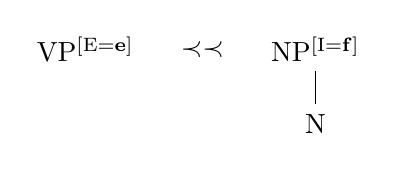
\begin{tikzpicture}[baseline]
\node at (0,0) (VP) {VP\textsuperscript{[E=\textbf{e}]}};
\node (follows) [right = 1em of VP] {$\prec\prec$};
\node [right = 1em of follows] (NP) {NP\textsuperscript{[I=\textbf{f}]}};
\node [below=\baselineskip of NP] (N) {N};
\draw (NP) -- (N);
\end{tikzpicture}
\end{minipage}
\caption{Temperature dimension constructor\label{app:temp}}
\end{figure}

\begin{figure}[H]
\begin{minipage}{0.5\textwidth}
\avm{
\btag{e} [\type*{event}
	\THEME & \btag{f} [\type*{entity}
       \AMOUNTDIM & \1
	]\\
\NOUNDIM & \1
]
}
\end{minipage}
\begin{minipage}{0.4\textwidth}
% % 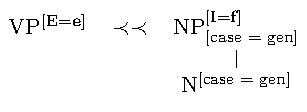
\includegraphics[scale=1]{NPgen.pdf}
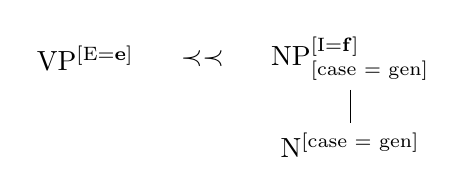
\begin{tikzpicture}[baseline]
\node at (0,0) (VP) {VP\textsuperscript{[E=\textbf{e}]}};
\node (follows) [right = 1em of VP] {$\prec\prec$};
\node [right = 1em of follows] (NP) {NP$^{\text{[I=\textbf{f}]}}_{\text{[case = gen]}}$};
\node [below=\baselineskip of NP] (N) {N\textsuperscript{[case = gen]}};
\draw (NP) -- (N);
\end{tikzpicture}
\end{minipage}
\caption{Amount dimension constructor \label{app:amount}}
\end{figure}

\begin{figure}[H]
\small
% \begin{minipage}{0.575\textwidth}
\avm{
\btag{e} [\type*{event}
	\THEME & \btag{f} [\type*{entity}
       \CARD & [\type*{cardinality}
       		\POS & \1
       	]
	]\\
\MDIM & [\type*{cardinality}
			\MIN & 0\\
       		\MAX & \1
       	]
]
}
% \end{minipage}
\hfill%
\begin{minipage}[c]{0.4\textwidth}
% % 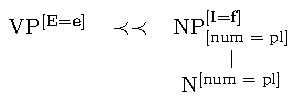
\includegraphics[scale=1]{NPpl.pdf}
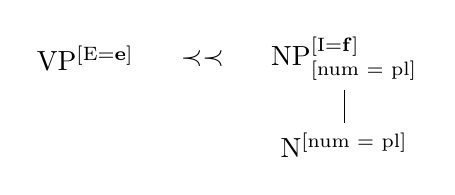
\begin{tikzpicture}[baseline]
\node at (0,0) (VP) {VP\textsuperscript{[E=\textbf{e}]}};
\node (follows) [right = 1em of VP] {$\prec\prec$};
\node [right = 1em of follows] (NP) {NP$^{\text{[I=\textbf{f}]}}_{\text{[num = pl]}}$};
\node [below=\baselineskip of NP] (N) {N\textsuperscript{[num = pl]}};
\draw (NP) -- (N);
\end{tikzpicture}
\end{minipage}
\caption{Cardinality dimension constructor \label{app:cardinality}}
\end{figure}

\begin{figure}[H]
\begin{minipage}{0.4\textwidth}
\avm{
\btag{e} [ \type*{event}
	\PATH & \1 [ \type*{path}
		\MIN & \2\\
		\MAX & \3
	]
]
}\\
\centering
\svar{1} $\in$ \svar{5} $\und$ \svar{2} $\in$ \svar{4} $\und$
\svar{3} $\in$ \svar{4}
\end{minipage}\hfill%
% \begin{minipage}{0.2\textwidth}
\avm{
\btag{f} [\type*{landmark}
       	\EDGE & \4 \\
       	\LOC & \5 ]
}\hfill%
% \end{minipage}
% \begin{minipage}{0.35\textwidth}
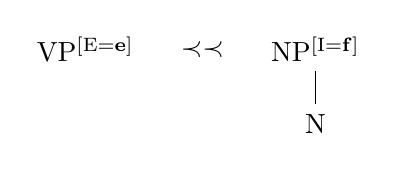
\begin{tikzpicture}[baseline]
\node at (0,0) (VP) {VP\textsuperscript{[E=\textbf{e}]}};
\node (follows) [right = 1em of VP] {$\prec\prec$};
\node [right = 1em of follows] (NP) {NP\textsuperscript{[I=\textbf{f}]}};
\node [below=\baselineskip of NP] (N) {N};
\draw (NP) -- (N);
\end{tikzpicture}
% \end{minipage}
\caption{Path dimension constructor \label{app:path}}
\end{figure}

\begin{figure}[H]
\small
\begin{minipage}{0.42\textwidth}
\avm{
\btag{e} [\type*{event}
	\NOUNDIM & [ \type*{time $\und$}\type*{one-point-scale}
			\MARKED & \1
	 ]
]
}
\end{minipage}
\begin{minipage}{0.18\textwidth}
\avm{
\btag{f} [\type*{entity}
       	\TIME & \1]
}
\end{minipage}
\begin{minipage}{0.35\textwidth}
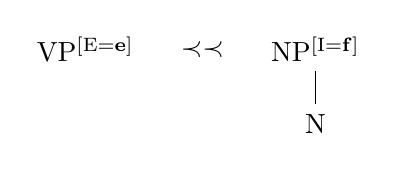
\begin{tikzpicture}[baseline]
\node at (0,0) (VP) {VP\textsuperscript{[E=\textbf{e}]}};
\node (follows) [right = 1em of VP] {$\prec\prec$};
\node [right = 1em of follows] (NP) {NP\textsuperscript{[I=\textbf{f}]}};
\node [below=\baselineskip of NP] (N) {N};
\draw (NP) -- (N);
\end{tikzpicture}
\end{minipage}
\caption{Time scale constructor: case of one marked point \label{app:time}}
\end{figure}

\begin{figure}[H]
% \begin{minipage}{0.7\textwidth}
\hfill\avm{
\btag{e}  [\type*{bounded-event}
     \MDIM & \3 [\type*{property-scale $\und$ closed-scale} 
		\MIN & \1\\
		\MAX & \2      
      ]\\
     \NOUNDIM & \3\\
     \INIT &  [\type*{stage}
     	\POS & \1]\\
     \FIN &  [\type*{stage}
     	\POS & \2]\\
  ]
 }\hfill%
%  \end{minipage}
%  \begin{minipage}{0.25\textwidth}
% %  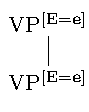
\includegraphics[scale=1]{VPcoerce.pdf}\hfill
\begin{forest}
[VP\textsuperscript{[E=\textbf{e}]}
  [VP\textsuperscript{[E=\textbf{e}]}]
]
\end{forest}\hfill
%  \end{minipage}
\caption{Frame and tree for coercion of an unbounded event into a bounded event \label{app:coerce}}
\end{figure}
	% Appendix Title
\chapter{XMG Implementation}\label{AppendixB}
\section{Current analysis}\label{B:me}
\begin{lstlisting}[style=AppendixStyle]
use unicity with (mark=anchor) dims (syn)
use unicity with (mark=nounacc) dims (syn)
use unicity with (iteration=yes) dims (syn)

type CAT={np, vp, s, n, v, det, pref, prep, suf, pp, pisat, zapisat,
				  rasskazy, vse, po-,pere-, do-, za-, iva-, vpfull}
type MARK={lex,anchor,coanchor,flex,nounacc}
type CASE={acc,gen,nom,inst}
type NUMBER={sg, pl}
type AGR !
type LABEL!
type ASP={perf, imperf}
type YES={yes,no}

feature cat: CAT
feature e: LABEL
feature i: LABEL
feature agr: AGR
feature case: CASE
feature gcase: CASE
feature num: NUMBER
feature aspect:ASP
feature bounded:YES
feature limited: YES
feature iteration: YES
property mark: MARK


frame-types = {event, scale, write, entity, object, story, bounded-event,
     					length, measure-of-change, proper-scale, iteration, 
     					property-scale, stage, cardinality, closed-scale, zero, 
     					process, record, progression, non-eventive}
    
frame-constraints = {
    event entity -> -,
    object -> entity,
    stage -> entity,
    story -> object,
    event zero -> -,
    zero entity -> -,
    scale entity -> -,
    scale zero -> -,

    bounded-event -> event,
    process -> event,
    iteration -> event,
    progression -> event,
    record -> event,

    closed-scale -> scale,
    measure-of-change -> closed-scale,
    cardinality -> closed-scale,
    proper-scale -> scale,
    proper-scale measure-of-change -> -,
    
    event cardinality -> iteration,
    length -> property-scale,
    cardinality property-scale -> -,
    property-scale -> scale,
    event property-scale -> -,
    property-scale proper-scale -> -,
    non-eventive event -> -,
    non-eventive -> scale,
    progression iteration -> -  
}

%%Lexical entries for the object 
class Story
export ?Length ?Card ?N
declare ?N ?Story ?X0 ?Length ?Card
{
  <syn>{
    node ?N (mark=coanchor) [cat=n, num = pl, i=?X0];
    node ?Story (mark=nounacc) [cat=rasskazy, num = pl, i=?X0];
    ?N -> ?Story
  };
  <frame>{
    ?X0[story,
        length: ?Length,
        cardinality: ?Card]
  }
}

%%Dimension constructors
class NounLength
export ?N ?NP ?VP
declare ?NLength ?X0 ?Length ?N ?NP ?VP ?Dim ?Theme ?Case ?Num
{
  ?NLength=Story[];
  ?NLength.?Length = ?Length;
  ?N=?NLength.?N;
  <syn>{
    node ?NP [cat=np, case=?Case, num = ?Num, i=?Theme];
    node ?VP [cat=vp, e=?X0];
    node ?N (mark=coanchor) [cat=n, case = ?Case, num = ?Num, i=?Theme];
    ?VP >>+ ?NP;
    ?NP -> ?N
  };
  <frame>{
    ?X0[event,
        theme:?Theme,
        noun-dim:[length,
                min:[zero],
                max:?Length]
    ]
  }
}

%% Plural nouns can be interpreted as introducing a cardinality scale
class NounCardinal
export ?N ?NP ?VP
declare ?NCard ?X0 ?Card ?N ?NP ?VP ?Dim ?Theme ?Case ?Num 
{
  ?NCard=Story[];
  ?NCard.?Card = ?Card;
  ?N=?NCard.?N;
    <syn>{
    node ?NP [cat=np, case=?Case, num = pl, i=?Theme];
    node ?VP [cat=vp, e=?X0, iteration = yes];
    node ?N (mark=coanchor) [cat=n, case = ?Case, num = pl, i=?Theme];
    ?VP >>+ ?NP;
    ?NP -> ?N
  };
  <frame>{
    ?X0[iteration,
        theme:?Theme,
        m-dim:[cardinality,
                min:[zero],
                max:?Card]
    ]
  }
}

%% NP -> m-dim
class NDim
export ?NP ?N ?VP
declare ?VP ?NP ?N ?Noun
{
  {?Noun=NounCardinal[] | ?Noun=NounLength[]};
  ?N=?Noun.?N;
  ?NP = ?Noun.?NP;
  ?VP = ?Noun.?VP
}

%Lexical entries for verbs
class Zapisat
export ?VP ?VPInt ?VPBase
declare ?V ?Pisat ?Za ?ZaLex ?X0 ?Actor ?Theme ?ScMin ?ScMax 
?AGR ?VP ?VPInt ?VPBase ?MDim
{
   ?VPBase = ?VPInt;
   <syn>{
    node ?VP [cat=vp, agr=?AGR, e=?X0, bounded = yes, 
    				limited = yes, aspect = perf];
    node ?V (mark=anchor) [cat=v, agr=?AGR, bounded = no, 
    				limited = no, aspect = imperf];
    node ?Pisat (mark=flex) [cat=pisat, agr=?AGR, bounded = no, 
    				limited = no, aspect = imperf];
    node ?Za [cat=pref];
    node ?ZaLex (mark=flex) [cat=za-];
    node ?VPInt [cat=vp, agr=?AGR, e=?X0, aspect = perf, bounded = yes];
    ?VP -> ?VPInt;
    ?VPInt -> ?V;
    ?VP -> ?Za;
    ?Za -> ?ZaLex;
    ?Za >> ?VPInt;
    ?V -> ?Pisat
  };
  <frame>{
    ?X0[bounded-event & process,
        actor:?Actor,
        theme:?Theme,
        manner:[record],
        verb-dim:?X0,
        noun-dim:?MDim [property-scale,
          min: ?ScMin,
          max: ?ScMax],
        m-dim:?MDim,
        init: [stage, 
          scale-deg:?ScMin],
        fin: [stage, 
          scale-deg:?ScMax]
    ]
  }
}

class Pisat
export ?V
declare ?V ?Pisat ?X0 ?Actor ?Theme
{
  <syn>{
    node ?V (mark=anchor) [cat=v, e=?X0, bounded = no, 
    		limited = no, aspect = imperf];
    node ?Pisat (mark=flex) [cat=pisat, e=?X0, bounded = no, 
    		limited = no, aspect = imperf];
    ?V -> ?Pisat
  };
  <frame>{
    ?X0[event & process,
        actor:?Actor,
        theme:?Theme,
        manner:[write],
        verb-dim:?X0[scale]
    ]
  }
}

%Creating the minimal VP and filling the verbal slot
class VSpine
export ?VP ?VPInt
declare ?VP ?V ?AGR ?X0 ?K ?VPInt ?Asp ?VLex ?A ?Lim 
{
  ?VPInt = ?VP;
  ?VLex = Pisat[];
  ?V = ?VLex.?V;
  <syn>{
    node ?VP [cat=vp, agr=?AGR, e=?X0, bounded = ?Asp, aspect = ?A, 
    		limited = ?Lim];
    node ?V (mark=anchor) [cat=v, agr=?AGR, e=?X0, bounded = ?Asp, 
    		aspect = ?A, limited = ?Lim];
    ?VP -> ?V
  } 
}

%%%%%%%%%%%%%%%%%%%%%%%%%%%%%
%Constructions associated with prefixes
%%%%%%%%%%%%%%%%%%%%%%%%%%%%%

%"Delimitative" and distributive po-
class PoVerb
export ?VP ?VPInt
declare ?VP ?VPInt ?Po ?PoLex ?AGR ?X0 ?Init ?Fin ?VDim
{
  <syn>{
    node ?VP [cat=vp, agr=?AGR, e=?X0, limited = yes, 
    		bounded = no, aspect = perf];
    node ?Po [cat=pref];
    node ?PoLex (mark=flex) [cat=po-];
    node ?VPInt [cat=vp, agr=?AGR, e=?X0, bounded = no];
    ?VP -> ?VPInt;
    ?VP -> ?Po;
    ?Po -> ?PoLex;
    ?Po >> ?VPInt
  };
  <frame>{
    ?X0[bounded-event,
       m-dim:?VDim[scale],
       verb-dim: ?VDim,
       init: [stage, 
          scale-deg:?Init],
       fin: [stage, 
          scale-deg:?Fin]
    ]
  }
}

class PereVerb
export ?VP ?VPInt 
declare ?VP ?VPInt ?Pere ?PereLex ?AGR ?X0 ?ScMin ?ScMax ?MDim
{
  <syn>{
    node ?VP [cat=vp, agr=?AGR, e=?X0, bounded = yes, 
    				 limited = yes, aspect = perf];
    node ?Pere [cat=pref];
    node ?PereLex (mark=flex) [cat=pere-];
    node ?VPInt [cat=vp, agr=?AGR, e=?X0, bounded = no];
    ?VP -> ?VPInt;
    ?VP -> ?Pere;
    ?Pere -> ?PereLex;
    ?Pere >> ?VPInt
  };
  <frame>{
    ?X0[bounded-event,
       m-dim: ?MDim[proper-scale,
          min: ?ScMin,
          max: ?ScMax],
       init: [stage, 
          scale-deg:?ScMin],
       fin: [stage, 
          scale-deg:?ScMax],
       noun-dim:?MDim
    ]
  }
}

%% Repetitive pere- 
class PereIterVerb
export ?VP ?VPInt 
declare ?VP ?VPInt ?Pere ?PereLex ?AGR ?X0 ?X1 ?Deg1 ?Deg2 
			?Scale ?NounDim ?Aspect ?EventType ?Init ?Fin ?Asp
{
  <syn>{
    node ?VP [cat=vp, agr=?AGR, e=?X1, bounded = ?Asp, 
    	limited = yes, aspect = ?Aspect];
    node ?Pere [cat=pref];
    node ?PereLex (mark=flex) [cat=pere-];
    node ?VPInt [cat=vp, agr=?AGR, e=?X0, bounded = ?Asp, 
    	limited = yes, aspect = ?Aspect];
    ?VP -> ?VPInt;
    ?VP -> ?Pere;
    ?Pere -> ?PereLex;
    ?Pere >> ?VPInt
  };
  <frame>{
    ?X1[?EventType,
       m-dim:?Scale[property-scale],
       noun-dim:?NounDim,
       init: ?Init,
       fin: ?Fin,
       prep:?X0[?EventType,
          m-dim:?Scale,
          noun-dim:?NounDim,
          init: ?Init,
          fin: ?Fin]
    ]
  }
}

class DoVerb
export ?VP ?VPInt 
declare ?VP ?VPInt ?Do ?DoLex ?AGR ?X0 ?X1 ?Deg1 ?Deg2 ?Deg3 
			?NDimType ?VDimType ?NDim ?VDim ?MDim
{
  <syn>{
    node ?VP [cat=vp, agr=?AGR, e=?X1, bounded = yes, 
    			limited = yes, aspect = perf];
    node ?Do [cat=pref];
    node ?DoLex (mark=flex) [cat=do-];
    node ?VPInt [cat=vp, agr=?AGR, e=?X0, limited = yes];
    ?VP -> ?VPInt;
    ?VP -> ?Do;
    ?Do -> ?DoLex;
    ?Do >> ?VPInt
  };
  <frame>{
    ?X1[bounded-event,
       m-dim:[closed-scale,
          min: ?Deg1,
          max: ?Deg2],
      fin:[stage, 
          scale-deg:?Deg2],
      init: [stage,
        scale-deg:?Deg3],
      part-of: ?X0
    ];
    ?X0[bounded-event,
       init: [stage, 
          scale-deg:?Deg1],
       fin: [stage, 
          scale-deg:?Deg2],
       m-dim: [non-eventive]
     ]
  }
}
    
    
%% Coersion: allows to create bounded events out of unbounded events
class NDimCoercedVerb
export ?VP ?VPInt
declare ?VP ?AGR ?X0 ?ScMin ?ScMax ?NounDim ?VPInt
{
  <syn>{
    node ?VP [cat=vp, agr=?AGR, e=?X0, bounded = yes,
    				 limited = yes, aspect = perf];
    node ?VPInt [cat=vp, agr=?AGR, e=?X0, limited = no, aspect = imperf];
    ?VP -> ?VPInt
  };
  <frame>{
    ?X0[bounded-event,
       m-dim: ?NounDim[property-scale & closed-scale,
          min: ?ScMin,
          max: ?ScMax],
       noun-dim:?NounDim,
       init:[stage, 
          scale-deg:?ScMin],
       fin:[stage, 
          scale-deg:?ScMax]
    ]
  }
}

%%%%%%%%%%%%%%%%%%%%%%%%%%%
%Imperfective suffix
%%%%%%%%%%%%%%%%%%%%%%%%%%%

%With iterative meaning
class IterVerb
export ?VP ?VPInt
declare ?VP ?VPInt ?Suf ?Iva ?AGR ?X0 ?X1 ?VDim
{
  <syn>{
    node ?VP [cat=vp, agr=?AGR, e=?X1, bounded = no, limited = no, 
    	aspect = imperf, iteration = yes];
    node ?Suf [cat=suf];
    node ?Iva (mark=flex) [cat=iva-];
    node ?VPInt [cat=vp, agr=?AGR, e=?X0, limited = yes];
    ?VP -> ?VPInt;
    ?VP -> ?Suf;
    ?Suf -> ?Iva;
    ?VPInt >> ?Suf
  };
  <frame>{
    ?X1[event & iteration,
       segment:?X0[bounded-event,
         noun-dim:[property-scale],
         verb-dim: ?VDim],
       verb-dim: ?VDim,
       noun-dim:[cardinality]
    ]
  }
}

%With progressive meaning
class ProgrVerb
export ?VP ?VPInt 
declare ?VP ?VPInt ?Suf ?Iva ?AGR ?X0 ?X1 ?NounDim ?VDim
{
  <syn>{
    node ?VP [cat=vp, agr=?AGR, e=?X1, bounded = no, 
    				 limited = yes, aspect = imperf];
    node ?Suf [cat=suf];
    node ?Iva (mark=flex) [cat=iva-];
    node ?VPInt [cat=vp, agr=?AGR, e=?X0, bounded = yes];
    ?VP -> ?VPInt;
    ?VP -> ?Suf;
    ?Suf -> ?Iva;
    ?VPInt >> ?Suf
  };
  <frame>{
  ?X1 [event & progression,
    part-of:?X0[bounded-event,
            noun-dim: ?NounDim,
            verb-dim: ?VDim],
    noun-dim: ?NounDim,
    verb-dim: ?VDim
    ]
  }
}

%%%%%%%%%%%%%%%%%%%%%%%
%Gathering verbs with one prefix

class OneBasePrefixedVerb
export ?VP ?VPInt ?VPBase
declare ?VP ?VPpref ?VSp ?VPInt ?VP ?AGR ?X0 ?VPBase
{
  {?VPpref = DoVerb[] | ?VPpref = PereVerb[] | 
   ?VPpref = PereIterVerb[] | ?VPpref = PoVerb[]};
  ?VP = ?VPpref.?VP;
  ?VSp = VSpine[];
  ?VPInt = ?VSp.?VP;
  ?VPInt = ?VPpref.?VPInt;
  ?VPBase = ?VPInt
}

class OneCoercedPrefixedVerb
export ?VP ?VPInt ?VPBase
declare ?VP ?VPpref ?VSp ?VPInt ?AGR ?X0 ?VPBase ?VCoerce 
{
  {?VPpref = DoVerb[] | ?VPpref = PereIterVerb[]};
  ?VP = ?VPpref.?VP;
  ?VSp = VSpine[];
  ?VCoerce = NDimCoercedVerb[];
  ?VPInt = ?VCoerce.?VP;
  ?VPInt = ?VPpref.?VPInt;
  ?VCoerce.?VPInt = ?VSp.?VP;
  ?VPBase = ?VPInt
}

class VerbWithOnePrefix
export ?VP ?VPInt ?VPBase
declare ?Verb ?VP ?VPInt ?VPBase
{
    {?Verb = OneBasePrefixedVerb[] | ?Verb = OneCoercedPrefixedVerb[] 
     | ?Verb = Zapisat[]};
    ?VP = ?Verb.?VP;
    ?VPInt = ?Verb.?VPInt;
    ?VPBase = ?Verb.?VPBase
}


%%%%%%%%%%%%%%%%%%%%%%%%%%
%Assembling multiply prefixed-suffixed verbs

%Stacking the second prefix above the first
class TwoPrefixedVerb
export ?VP ?VPInt ?VPBase
declare ?VP ?VPpref ?V ?VSp ?VPInt ?VP ?VPBase
{
  {?VPpref = DoVerb[] | ?VPpref = PereVerb[] | 
  	?VPpref = PereIterVerb[] | ?VPpref = PoVerb[]};
  ?VP = ?VPpref.?VP;
  ?VSp = VerbWithOnePrefix[];
  ?VPInt = ?VSp.?VP;
  ?VPInt = ?VPpref.?VPInt;
  ?VPBase = ?VSp.?VPBase
}

%Adding imperfective suffix
class SuffVerb
export ?VP ?VPInt ?VPBase ?NP ?VPFin ?VPBaseOld
declare ?VP ?VPInt ?Suf ?VPBaseOld ?VPBase ?Verb ?NP ?Noun ?VPFin 
{
  {?Verb = VerbWithOnePrefix[] | ?Verb = TwoPrefixedVerb[]};
  ?VPInt = ?Verb.?VP;
  ?VPBaseOld = ?Verb.?VPBase;
  {?Suf =  ProgrVerb[] | ?Suf = IterVerb[]};
  ?VP = ?Suf.?VP;
  ?VPInt = ?Suf.?VPInt;
  ?VPBase = ?VP;
  ?Noun = NDim[];
  ?NP = ?Noun.?NP;
  ?VPBaseOld = ?Noun.?VP;
  <syn>{
    node ?VPFin [cat = vpfull];
    ?VPFin ->+ ?VP;
    ?VPFin -> ?NP
    }
}

%%%%%%%%%%%%%%%%%%%%%%%%
%Checking that types are inherited
class TypeMatcher
export ?VPOut ?VPInt
declare ?VPInt ?X0 ?X1 ?NDimType ?VDimType ?MDim ?VPOut
{
<syn>{
    node ?VPOut [e=?X1];
    node ?VPInt [e=?X0]
    };
  <frame>{
    ?X1[event,
       m-dim: [?MDim],
       noun-dim: [?NDimType],
       verb-dim: [?VDimType]
    ];
    ?X0[event,
       m-dim: [?MDim],
       noun-dim: [?NDimType],
       verb-dim: [?VDimType]
     ]
  }
}

class SuffTyped
export ?VP ?VPBase ?NP ?VPFin 
declare ?VP ?VPInt ?Suf ?VPBaseOld ?VPBase ?NP ?Verb ?VPFin 
		?X0 ?X1 ?NDimType ?VDimType ?MDim ?Typing ?VPOut
{
    ?Verb = SuffVerb[];
    ?Typing = TypeMatcher[];
    ?VPInt = ?Verb.?VPInt;
    ?VPInt = ?Typing.?VPInt;
    ?VPOut = ?Verb.?VPBaseOld;
    ?VPOut = ?Typing.?VPOut;
    ?VPBase = ?Verb.?VPBase;
    ?NP = ?Verb.?NP;
    ?VPFin = ?Verb.?VPFin;
    ?VP = ?Verb.?VP
}

%%%%%%%%%%%%%%%%%%%%%%%%%%
%Stacking the another prefix above the suffix

class TwoPrefixedSuffixedVerb
export ?VP ?VPInt ?VPBase ?NP ?VPFin
declare ?VP ?VPpref ?V ?VSp ?VPInt ?VP ?AGR ?X0 ?VPBase ?NP ?VPFin
{
  {?VPpref = DoVerb[] | ?VPpref = PereVerb[] 
  | ?VPpref = PereIterVerb[] | ?VPpref = PoVerb[]};
  ?VP = ?VPpref.?VP;
  ?VSp = SuffTyped[];
  ?VPInt = ?VSp.?VP;
  ?VPInt = ?VPpref.?VPInt;
  ?VPBase = ?VSp.?VPBase;
  ?VPFin = ?VSp.?VPFin;
  ?NP = ?VSp.?NP
}

%%%%%%%%%%%%%%%%%%%%%%%%%%%
%Assembling the direct object 

class PrefixedVerbDirObj
export ?VPFin ?NP ?VPBase
declare ?VP ?VPpref ?V ?VSp ?VPInt ?VP ?AGR ?X0 ?X1 ?NP 
			?VPFin ?Noun ?VPBase ?ASP ?NDimType ?VDimType ?MDim
{
  ?Noun = NDim[];
  ?NP = ?Noun.?NP;
  {?VPpref = VerbWithOnePrefix[]| ?VPpref = TwoPrefixedVerb[]};
  ?VP = ?VPpref.?VP;
  ?VPBase = ?Noun.?VP;
  ?VPBase = ?VPpref.?VPBase;
  ?VPInt = ?VPpref.?VPInt;
  <syn>{
  node ?VPFin [cat = vpfull, agr = ?AGR, aspect = ?ASP, e = ?X1];
  node ?VP [cat = vp, agr = ?AGR, aspect = ?ASP, e = ?X1];
  node ?VPBase [e=?X0];
  node ?NP [case = acc];
  ?VPFin -> ?VP;
  ?VPFin -> ?NP
  }
}

class PrefixedSuffixedVerbDirObj
export ?VPFin ?NP ?VPBase
declare ?VP ?VPpref ?V ?VSp ?VPInt ?VP ?AGR ?X0 
			?NP ?VPFin ?Noun ?VPBase ?ASP ?X0 
{
  ?Noun = NDim[];
  ?NP = ?Noun.?NP;
  ?VPpref = TwoPrefixedSuffixedVerb[];
  ?VP = ?VPpref.?VP;
  ?VPBase = ?Noun.?VP;
  ?VPBase = ?VPpref.?VPBase;
  ?VPInt = ?VPpref.?VPInt;
  ?NP = ?VPpref.?NP;
  ?VPFin = ?VPpref.?VPFin;
  <syn>{
  node ?VPFin [cat = vpfull, agr = ?AGR, aspect = ?ASP, e = ?X0];
  node ?VP [cat = vp, agr = ?AGR, aspect = ?ASP, e = ?X0];
  node ?NP [case = acc];
  ?VPFin -> ?VP;
  ?VPFin -> ?NP
  }
}

%%%%%%%%%%%%%%%%%%%%%%%%%%%
%Matching types again
class PrefTyped
export ?NP ?VPFin ?VPBase ?VP
declare ?VP ?VPInt ?VPBase ?NP ?Verb ?VPFin ?X0 ?X1 
			?NDimType ?VDimType ?MDim ?Typing ?VPOut
{
    {?Verb = PrefixedVerbDirObj[]|?Verb = PrefixedSuffixedVerbDirObj[]};
    ?Typing = TypeMatcher[];
    ?VPInt = ?Verb.?VPBase;
    ?VPInt = ?Typing.?VPInt;
    ?VPOut = ?Verb.?VPFin;
    ?VPOut = ?Typing.?VPOut;
    ?NP = ?Verb.?NP;
    ?VPFin = ?Verb.?VPFin;
    ?VPBase = ?Verb.?VPBase;
    ?VP = ?VPFin
}

%%%%%%%%%%%%%%%%%%%%%%%%%%%
%Assembling the results in one class
class AllVerbs
declare ?Verb
{
    {?Verb = PrefTyped[] | ?Verb = SuffTyped[]}
}

value AllVerbs

\end{lstlisting}

\section{Analysis proposed by \citet{Tatevosov:09}}\label{B:Tat}
\begin{lstlisting}[style=AppendixStyle]
use unicity with (mark=anchor) dims (syn)

type CAT={vp,v,det,pref,suf,pisat,zapisat, po-,pere-,do-,za-,iva-}
type MARK={lex,anchor, flex}
type CASE={acc,gen,nom,inst}
type AGR !
type LABEL!
type A={perf, imperf}

feature cat: CAT
feature e: LABEL
feature agr: AGR
feature gcase: CASE
feature aspect:A
property mark: MARK

frame-types = {write, write-down, distributive, delimitative, 
	completive, iteration, imperfective, repetitive}
frame-constraints = {
write write-down -> -,
distributive delimitative -> -,
completive delimitative -> -,
distributive iteration -> -,
distributive repetitive -> -
}

%%Lexical entries for verbs
class Zapisat
export ?VP ?VPInt
declare ?V ?Pisat ?Za ?ZaLex ?X0 ?AGR ?VP ?VPInt
{
   <syn>{
    node ?VP [cat=vp, agr=?AGR, e=?X0, aspect = perf];
    node ?V (mark=anchor) [cat=v, agr=?AGR, aspect = imperf];
    node ?Pisat (mark=flex) [cat=pisat, agr=?AGR, aspect = imperf];
    node ?Za [cat=pref];
    node ?ZaLex (mark=flex) [cat=za-];
    node ?VPInt [cat=vp, agr=?AGR, e=?X0, aspect = perf];
    ?VP -> ?VPInt;
    ?VPInt -> ?V;
    ?VP -> ?Za;
    ?Za -> ?ZaLex;
    ?Za >> ?VPInt;
    ?V -> ?Pisat
  };
  <frame>{
    ?X0[write-down]
  }
}

class Pisat
export ?V
declare ?V ?Pisat ?X0
{
  <syn>{
    node ?V (mark=anchor) [cat=v, e=?X0, aspect = imperf];
    node ?Pisat (mark=flex) [cat=pisat, e=?X0,  aspect = imperf];
    ?V -> ?Pisat
  };
  <frame>{
    ?X0[write]
  }
}

%Creating the minimal VP and filling the verbal slot
class VSpine
export ?VP ?VPInt
declare ?VP ?V ?AGR ?X0 ?K ?VPInt ?Asp ?VLex ?A
{
  ?VPInt = ?VP;
  ?VLex = Pisat[];
  ?V = ?VLex.?V;
  <syn>{
    node ?VP [cat=vp, agr=?AGR, e=?X0,  aspect = ?A];
    node ?V (mark=anchor) [cat=v, agr=?AGR, e=?X0,  aspect = ?A];
    ?VP -> ?V
  } 
}

%%%%%%%%%%%%%%%%%%%%%%%%%%%%%%%%%%%
%%Constructions associated with prefixes
%%"Delimitative" po-
class PoVerb
export ?VP ?VPInt
declare ?VP ?VPInt ?Po ?PoLex ?AGR ?X0 ?X1
{
  <syn>{
    node ?VP [cat=vp, agr=?AGR, e=?X1, aspect = perf];
    node ?Po [cat=pref];
    node ?PoLex (mark=flex) [cat=po-];
    node ?VPInt [cat=vp, agr=?AGR, e=?X0, aspect=imperf];
    ?VP -> ?VPInt;
    ?VP -> ?Po;
    ?Po -> ?PoLex;
    ?Po >> ?VPInt
  };
  <frame>{
    ?X1[delimitative,
       of: ?X0]
  }
}

class PoDistrVerb
export ?VP ?VPInt
declare ?VP ?VPInt ?Po ?PoLex ?AGR ?X0 ?X1
{
  <syn>{
    node ?VP [cat=vp, agr=?AGR, e=?X1, aspect = perf];
    node ?Po [cat=pref];
    node ?PoLex (mark=flex) [cat=po-];
    node ?VPInt [cat=vp, agr=?AGR, e=?X0];
    ?VP -> ?VPInt;
    ?VP -> ?Po;
    ?Po -> ?PoLex;
    ?Po >> ?VPInt
  };
  <frame>{
    ?X1[distributive,
       of: ?X0]
  }
}

class PereVerb
export ?VP ?VPInt 
declare ?VP ?VPInt ?Pere ?PereLex ?AGR ?X0 ?X1 
{
  <syn>{
    node ?VP [cat=vp, agr=?AGR, e=?X1, aspect = perf];
    node ?Pere [cat=pref];
    node ?PereLex (mark=flex) [cat=pere-];
    node ?VPInt [cat=vp, agr=?AGR, e=?X0, aspect = imperf];
    ?VP -> ?VPInt;
    ?VP -> ?Pere;
    ?Pere -> ?PereLex;
    ?Pere >> ?VPInt
  };
  <frame>{
    ?X1[distributive,
       of: ?X0]
  }
}

%% Repetitive pere- 
class PereIterVerb
export ?VP ?VPInt 
declare ?VP ?VPInt ?Pere ?PereLex ?AGR ?X0 ?X1 
{
  <syn>{
    node ?VP [cat=vp, agr=?AGR, e=?X1, aspect = perf];
    node ?Pere [cat=pref];
    node ?PereLex (mark=flex) [cat=pere-];
    node ?VPInt [cat=vp, agr=?AGR, e=?X0];
    ?VP -> ?VPInt;
    ?VP -> ?Pere;
    ?Pere -> ?PereLex;
    ?Pere >> ?VPInt
  };
  <frame>{
    ?X1[repetitive,
        of: ?X0]
  }
}

class DoVerb
export ?VP ?VPInt 
declare ?VP ?VPInt ?Do ?DoLex ?AGR ?X0 ?X1 
{
  <syn>{
    node ?VP [cat=vp, agr=?AGR, e=?X1, aspect = perf];
    node ?Do [cat=pref];
    node ?DoLex (mark=flex) [cat=do-];
    node ?VPInt [cat=vp, agr=?AGR, e=?X0];
    ?VP -> ?VPInt;
    ?VP -> ?Do;
    ?Do -> ?DoLex;
    ?Do >> ?VPInt
  };
  <frame>{
    ?X1[completive,
      of:?X0]
  }
}

%%%%%%%%%%%%%%%%%%%%%%%%%%%%%%%%
%%Gathering verbs with one prefix
class OneBasePrefixedVerb
export ?VP ?VPInt
declare ?VP ?VPpref ?VSp ?VPInt ?VP ?AGR ?X0
{
  {?VPpref = DoVerb[] | ?VPpref = PereVerb[] | ?VPpref = PereIterVerb[] | 
  		?VPpref = PoVerb[]};
  ?VP = ?VPpref.?VP;
  ?VSp = VSpine[];
  ?VPInt = ?VSp.?VP;
  ?VPInt = ?VPpref.?VPInt
}

class VerbWithOnePrefix
export ?VP ?VPInt
declare ?Verb ?VP ?VPInt
{
    {?Verb = OneBasePrefixedVerb[] | ?Verb = Zapisat[]};
    ?VP = ?Verb.?VP;
    ?VPInt = ?Verb.?VPInt
}

%%%%%%%%%%%%%%%%%%%%%%%%%%%%%%%%%%
%%Assembling multiply prefixed-suffixed verbs
%%Stacking the second prefix above the first

class TwoPrefixedVerb
export ?VP ?VPInt
declare ?VP ?VPpref ?V ?VSp ?VPInt ?VP ?AGR ?X0
{
  {?VPpref = DoVerb[] | ?VPpref = PereVerb[] | 
  	?VPpref = PereIterVerb[] | ?VPpref = PoVerb[]};
  ?VP = ?VPpref.?VP;
  ?VSp = VerbWithOnePrefix[];
  ?VPInt = ?VSp.?VP;
  ?VPInt = ?VPpref.?VPInt
}

%%Adding imperfective suffix
class ImpVerb
export ?VP ?VPInt
declare ?VP ?VPInt ?Suf ?Iva ?AGR ?X0 ?X1
{
  <syn>{
    node ?VP [cat=vp, agr=?AGR, e=?X1, aspect = imperf];
    node ?Suf [cat=suf];
    node ?Iva (mark=flex) [cat=iva-];
    node ?VPInt [cat=vp, agr=?AGR, e=?X0];
    ?VP -> ?VPInt;
    ?VP -> ?Suf;
    ?Suf -> ?Iva;
    ?VPInt >> ?Suf
  };
  <frame>{
    ?X1[imperfective,
       of:?X0]
  }
}

%%Assembling suffixed verb
class SuffVerb
export ?VP ?VPInt 
declare ?VP ?VPInt ?Suf ?X0 ?X1 ?X2 ?X3 ?Verb 
{
  {?Verb = VerbWithOnePrefix[] | ?Verb = TwoPrefixedVerb[]};
  ?VPInt = ?Verb.?VP;
  ?Suf =  ImpVerb[];
  ?VP = ?Suf.?VP;
  ?VPInt = ?Suf.?VPInt
}

%%Stacking the another prefix above the suffix
class PrefixedSuffixedVerb
export ?VP ?VPInt
declare ?VP ?VPpref ?V ?VSp ?VPInt ?VP ?AGR ?X0 
{
  {?VPpref = PereVerb[] | ?VPpref = PoVerb[]};
  ?VP = ?VPpref.?VP;
  ?VSp = SuffVerb[];
  ?VPInt = ?VSp.?VP;
  ?VPInt = ?VPpref.?VPInt
}

class AlmostAllVerbs
export ?VP ?VPInt
declare ?Verb ?VP ?VPInt
{
  {?Verb = VerbWithOnePrefix[] | ?Verb = SuffVerb[]};
  ?VP = ?Verb.?VP;
  ?VPInt = ?Verb.?VPInt
}

class PoDistrPrefixedVerb
export ?VP ?VPInt
declare ?VP ?VPpref ?V ?VSp ?VPInt ?VP ?AGR ?X0
{
  ?VPpref = PoDistrVerb[];
  ?VP = ?VPpref.?VP;
  {?VSp = AlmostAllVerbs[] | ?VSp = VSpine[]};
  ?VPInt = ?VSp.?VP;
  ?VPInt = ?VPpref.?VPInt
}

class AllVerbs
declare ?Verb
{
  {?Verb = AlmostAllVerbs[] | ?Verb = PoDistrPrefixedVerb[] 
  | ?Verb = PrefixedSuffixedVerb[]  | ?Verb = TwoPrefixedVerb[]}
}

value AllVerbs
\end{lstlisting}
 % Appendix Title

%%%%%%%%%%%%%%%%%%%%%%%%%%%%%%%%%%%%%%%%%%%%%%%%%%%%
%%%                                              %%%
%%%             Backmatter                       %%%
%%%                                              %%%
%%%%%%%%%%%%%%%%%%%%%%%%%%%%%%%%%%%%%%%%%%%%%%%%%%%%

\is{some term| see {some other term}}
\il{some language| see {some other language}}
\issa{some term with pages}{some other term also of interest}
\ilsa{some language with pages}{some other lect also of interest} 
% There is normally no need to change the backmatter section
\backmatter

\phantomsection%this allows hyperlink in ToC to work
\printbibliography[heading=references] 
\cleardoublepage

\phantomsection 
\addcontentsline{toc}{chapter}{Index} 
\addcontentsline{toc}{section}{Name index}
\ohead{Name index} 
\printindex 
\cleardoublepage
  
%\phantomsection 
%\addcontentsline{toc}{section}{Language index}
%\ohead{Language index} 
%\printindex[lan] 
%\cleardoublepage
  
\phantomsection 
\addcontentsline{toc}{section}{Subject index}
\ohead{Subject index} 
\printindex[sbj]
\ohead{} 
 
\end{document} 

% you can create your book by running
% xelatex main.tex
%
% you can also try a simple 
% make
% on the commandline
